%%%%%%%%%%%%%%%%%%%%%%%%%%%%%%%%%%%%%%%%%
% The Legrand Orange Book
% LaTeX Template
% Version 2.0 (9/2/15)
%
% This template has been downloaded from:
% http://www.LaTeXTemplates.com
%
% Mathias Legrand (legrand.mathias@gmail.com) with modifications by:
% Vel (vel@latextemplates.com)
%
% License:
% CC BY-NC-SA 3.0 (http://creativecommons.org/licenses/by-nc-sa/3.0/)
%
% Compiling this template:
% This template uses biber for its bibliography and makeindex for its index.
% When you first open the template, compile it from the command line with the 
% commands below to make sure your LaTeX distribution is configured correctly:
%
% 1) pdflatex main
% 2) makeindex main.idx -s StyleInd.ist
% 3) biber main
% 4) pdflatex main x 2
%
% After this, when you wish to update the bibliography/index use the appropriate
% command above and make sure to compile with pdflatex several times 
% afterwards to propagate your changes to the document.
%
% This template also uses a number of packages which may need to be
% updated to the newest versions for the template to compile. It is strongly
% recommended you update your LaTeX distribution if you have any
% compilation errors.
%
% Important note:
% Chapter heading images should have a 2:1 width:height ratio,
% e.g. 920px width and 460px height.
%
%%%%%%%%%%%%%%%%%%%%%%%%%%%%%%%%%%%%%%%%%

%----------------------------------------------------------------------------------------
%	PACKAGES AND OTHER DOCUMENT CONFIGURATIONS
%----------------------------------------------------------------------------------------

\documentclass[11pt,fleqn]{book} % Default font size and left-justified equations

%----------------------------------------------------------------------------------------

%%%%%%%%%%%%%%%%%%%%%%%%%%%%%%%%%%%%%%%%%
% The Legrand Orange Book
% Structural Definitions File
% Version 2.0 (9/2/15)
%
% Original author:
% Mathias Legrand (legrand.mathias@gmail.com) with modifications by:
% Vel (vel@latextemplates.com)
% 
% This file has been downloaded from:
% http://www.LaTeXTemplates.com
%
% License:
% CC BY-NC-SA 3.0 (http://creativecommons.org/licenses/by-nc-sa/3.0/)
%
%%%%%%%%%%%%%%%%%%%%%%%%%%%%%%%%%%%%%%%%%

%----------------------------------------------------------------------------------------
%	VARIOUS REQUIRED PACKAGES AND CONFIGURATIONS
%----------------------------------------------------------------------------------------

% Page margins
% rleiva
\usepackage[top=3cm,bottom=3cm,left=3cm,right=3cm,headsep=10pt,a4paper]{geometry}
% B5
% \usepackage[top=2cm,bottom=2cm,left=2cm,right=2cm,headsep=10pt,b5paper]{geometry}
% Octavo
% \usepackage[paperheight=229mm, paperwidth=152mm, top=16mm, bottom=16mm, left=20mm, right=16mm, headsep={10pt}]{geometry}
% For tables
\usepackage{multirow}

\usepackage{graphicx} % Required for including pictures
\graphicspath{{Pictures/}} % Specifies the directory where pictures are stored

\usepackage{lipsum} % Inserts dummy text

\usepackage{tikz} % Required for drawing custom shapes
\usetikzlibrary{arrows} % rleiva
\usetikzlibrary{shapes} % rleiva

\usepackage[english]{babel} % English language/hyphenation

\usepackage{enumitem} % Customize lists
\setlist{nolistsep} % Reduce spacing between bullet points and numbered lists

\usepackage{booktabs} % Required for nicer horizontal rules in tables

\usepackage{xcolor} % Required for specifying colors by name
\definecolor{ocre}{RGB}{243,102,25} % Define the orange color used for highlighting throughout the book

% rleiva: for algorithms pseudocode
\usepackage{algpseudocode}
\usepackage[chapter]{algorithm}

% rleiva: for text wrapping around figures
\usepackage{wrapfig}

% rleiva: use Roman numbers in enumerations
\renewcommand{\labelenumi}{\theenumi}


%----------------------------------------------------------------------------------------
%	FONTS
%----------------------------------------------------------------------------------------

\usepackage{avant} % Use the Avantgarde font for headings
%\usepackage{times} % Use the Times font for headings
\usepackage{mathptmx} % Use the Adobe Times Roman as the default text font together with math symbols from the Sym­bol, Chancery and Com­puter Modern fonts

% rleiva
% mathptmx also changes the math fonts, but I want to keep the original \mathcal symbols
\DeclareMathAlphabet{\mathcal}{OMS}{cmsy}{m}{n}

\usepackage{microtype} % Slightly tweak font spacing for aesthetics
\usepackage[utf8]{inputenc} % Required for including letters with accents
\usepackage[T1]{fontenc} % Use 8-bit encoding that has 256 glyphs

%----------------------------------------------------------------------------------------
%	BIBLIOGRAPHY AND INDEX
%----------------------------------------------------------------------------------------

% rleiva
\usepackage[style=alphabetic,citestyle=alphabetic,sorting=nyt,sortcites=true,autopunct=true,babel=hyphen,hyperref=true,abbreviate=false,backref=true,backend=biber]{biblatex}
% \usepackage[style=alphabetic,citestyle=numeric,sorting=nyt,sortcites=true,autopunct=true,babel=hyphen,hyperref=true,abbreviate=false,backref=true,backend=biber]{biblatex}
\addbibresource{bibliography.bib} % BibTeX bibliography file
\defbibheading{bibempty}{}

\usepackage{calc} % For simpler calculation - used for spacing the index letter headings correctly
\usepackage{makeidx} % Required to make an index
\makeindex % Tells LaTeX to create the files required for indexing

%----------------------------------------------------------------------------------------
%	MAIN TABLE OF CONTENTS
%----------------------------------------------------------------------------------------

\usepackage{titletoc} % Required for manipulating the table of contents

\contentsmargin{0cm} % Removes the default margin

% Part text styling
\titlecontents{part}[0cm]
{\addvspace{20pt}\centering\large\bfseries}
{}
{}
{}

% Chapter text styling
\titlecontents{chapter}[1.25cm] % Indentation
{\addvspace{12pt}\large\sffamily\bfseries} % Spacing and font options for chapters
{\color{ocre!60}\contentslabel[\Large\thecontentslabel]{1.25cm}\color{ocre}} % Chapter number
{\color{ocre}}  
{\color{ocre!60}\normalsize\;\titlerule*[.5pc]{.}\;\thecontentspage} % Page number

% Section text styling
\titlecontents{section}[1.25cm] % Indentation
{\addvspace{3pt}\sffamily\bfseries} % Spacing and font options for sections
{\contentslabel[\thecontentslabel]{1.25cm}} % Section number
{}
{\hfill\color{black}\thecontentspage} % Page number
[]

% Subsection text styling
\titlecontents{subsection}[1.25cm] % Indentation
{\addvspace{1pt}\sffamily\small} % Spacing and font options for subsections
{\contentslabel[\thecontentslabel]{1.25cm}} % Subsection number
{}
{\ \titlerule*[.5pc]{.}\;\thecontentspage} % Page number
[]

% List of figures
\titlecontents{figure}[0em]
{\addvspace{-5pt}\sffamily}
{\thecontentslabel\hspace*{1em}}
{}
{\ \titlerule*[.5pc]{.}\;\thecontentspage}
[]

% List of tables
\titlecontents{table}[0em]
{\addvspace{-5pt}\sffamily}
{\thecontentslabel\hspace*{1em}}
{}
{\ \titlerule*[.5pc]{.}\;\thecontentspage}
[]

%----------------------------------------------------------------------------------------
%	MINI TABLE OF CONTENTS IN PART HEADS
%----------------------------------------------------------------------------------------

% Chapter text styling
\titlecontents{lchapter}[0em] % Indenting
{\addvspace{15pt}\large\sffamily\bfseries} % Spacing and font options for chapters
{\color{ocre}\contentslabel[\Large\thecontentslabel]{1.25cm}\color{ocre}} % Chapter number
{}  
{\color{ocre}\normalsize\sffamily\bfseries\;\titlerule*[.5pc]{.}\;\thecontentspage} % Page number

% Section text styling
\titlecontents{lsection}[0em] % Indenting
{\sffamily\small} % Spacing and font options for sections
{\contentslabel[\thecontentslabel]{1.25cm}} % Section number
{}
{}

% Subsection text styling
\titlecontents{lsubsection}[.5em] % Indentation
{\normalfont\footnotesize\sffamily} % Font settings
{}
{}
{}

%----------------------------------------------------------------------------------------
%	PAGE HEADERS
%----------------------------------------------------------------------------------------

\usepackage{fancyhdr} % Required for header and footer configuration

\pagestyle{fancy}
\renewcommand{\chaptermark}[1]{\markboth{\sffamily\normalsize\bfseries\chaptername\ \thechapter.\ #1}{}} % Chapter text font settings
\renewcommand{\sectionmark}[1]{\markright{\sffamily\normalsize\thesection\hspace{5pt}#1}{}} % Section text font settings
\fancyhf{} \fancyhead[LE,RO]{\sffamily\normalsize\thepage} % Font setting for the page number in the header
\fancyhead[LO]{\rightmark} % Print the nearest section name on the left side of odd pages
\fancyhead[RE]{\leftmark} % Print the current chapter name on the right side of even pages
\renewcommand{\headrulewidth}{0.5pt} % Width of the rule under the header
\addtolength{\headheight}{2.5pt} % Increase the spacing around the header slightly
\renewcommand{\footrulewidth}{0pt} % Removes the rule in the footer
\fancypagestyle{plain}{\fancyhead{}\renewcommand{\headrulewidth}{0pt}} % Style for when a plain pagestyle is specified

% Removes the header from odd empty pages at the end of chapters
\makeatletter
\renewcommand{\cleardoublepage}{
\clearpage\ifodd\c@page\else
\hbox{}
\vspace*{\fill}
\thispagestyle{empty}
\newpage
\fi}

%----------------------------------------------------------------------------------------
%	THEOREM STYLES
%----------------------------------------------------------------------------------------

\usepackage{amsmath,amsfonts,amssymb,amsthm} % For math equations, theorems, symbols, etc

\newcommand{\intoo}[2]{\mathopen{]}#1\,;#2\mathclose{[}}
\newcommand{\ud}{\mathop{\mathrm{{}d}}\mathopen{}}
\newcommand{\intff}[2]{\mathopen{[}#1\,;#2\mathclose{]}}
\newtheorem{notation}{Notation}[chapter]

% rleiva: we need the argmin and argmax operators
\DeclareMathOperator*{\argmin}{arg\,min}
\DeclareMathOperator*{\argmax}{arg\,max}

% Boxed/framed environments
\newtheoremstyle{ocrenumbox}% % Theorem style name
{0pt}% Space above
{0pt}% Space below
{\normalfont}% % Body font
{}% Indent amount
{\small\bf\sffamily\color{ocre}}% % Theorem head font
{\;}% Punctuation after theorem head
{0.25em}% Space after theorem head
{\small\sffamily\color{ocre}\thmname{#1}\nobreakspace\thmnumber{\@ifnotempty{#1}{}\@upn{#2}}% Theorem text (e.g. Theorem 2.1)
\thmnote{\nobreakspace\the\thm@notefont\sffamily\bfseries\color{black}---\nobreakspace#3.}} % Optional theorem note
\renewcommand{\qedsymbol}{$\blacksquare$}% Optional qed square

\newtheoremstyle{blacknumex}% Theorem style name
{5pt}% Space above
{5pt}% Space below
{\normalfont}% Body font
{} % Indent amount
{\small\bf\sffamily}% Theorem head font
{\;}% Punctuation after theorem head
{0.25em}% Space after theorem head
{\small\sffamily{\tiny\ensuremath{\blacksquare}}\nobreakspace\thmname{#1}\nobreakspace\thmnumber{\@ifnotempty{#1}{}\@upn{#2}}% Theorem text (e.g. Theorem 2.1)
\thmnote{\nobreakspace\the\thm@notefont\sffamily\bfseries---\nobreakspace#3.}}% Optional theorem note

\newtheoremstyle{blacknumbox} % Theorem style name
{0pt}% Space above
{0pt}% Space below
{\normalfont}% Body font
{}% Indent amount
{\small\bf\sffamily}% Theorem head font
{\;}% Punctuation after theorem head
{0.25em}% Space after theorem head
{\small\sffamily\thmname{#1}\nobreakspace\thmnumber{\@ifnotempty{#1}{}\@upn{#2}}% Theorem text (e.g. Theorem 2.1)
\thmnote{\nobreakspace\the\thm@notefont\sffamily\bfseries---\nobreakspace#3.}}% Optional theorem note

% rleiva: create source code box
\newtheoremstyle{sourcecodebox} % Theorem style name
{0pt}% Space above
{0pt}% Space below
{\normalfont}% Body font
{}% Indent amount
{\small\bf\sffamily}% Theorem head font
{}% Punctuation after theorem head
{0em}% Space after theorem head
% {\small\sffamily\thmname{#1}\nobreakspace% Theorem text (e.g. Theorem 2.1)
% \thmnote{\nobreakspace\the\thm@notefont\sffamily\bfseries---\nobreakspace#3.}}% Optional theorem note

% Non-boxed/non-framed environments
\newtheoremstyle{ocrenum}% % Theorem style name
{5pt}% Space above
{5pt}% Space below
{\normalfont}% % Body font
{}% Indent amount
{\small\bf\sffamily\color{ocre}}% % Theorem head font
{\;}% Punctuation after theorem head
{0.25em}% Space after theorem head
{\small\sffamily\color{ocre}\thmname{#1}\nobreakspace\thmnumber{\@ifnotempty{#1}{}\@upn{#2}}% Theorem text (e.g. Theorem 2.1)
\thmnote{\nobreakspace\the\thm@notefont\sffamily\bfseries\color{black}---\nobreakspace#3.}} % Optional theorem note
\renewcommand{\qedsymbol}{$\blacksquare$}% Optional qed square
\makeatother

% Defines the theorem text style for each type of theorem to one of the three styles above
\newcounter{dummy} 
\numberwithin{dummy}{section}
\theoremstyle{ocrenumbox}
\newtheorem{theoremeT}[dummy]{Theorem}
\newtheorem{problem}{Problem}[chapter]
\newtheorem{exerciseT}{Exercise}[chapter]
\theoremstyle{blacknumex}
\newtheorem{exampleT}{Example}[chapter]
\theoremstyle{blacknumbox}
\newtheorem{vocabulary}{Vocabulary}[chapter]
\newtheorem{definitionT}{Definition}[section]
\newtheorem{corollaryT}[dummy]{Corollary}

\theoremstyle{sourcecodebox}
% rleiva: create source code box
\newtheorem{sourcecodeT}[dummy]{}

\theoremstyle{ocrenum}
\newtheorem{proposition}[dummy]{Proposition}

%----------------------------------------------------------------------------------------
%	DEFINITION OF COLORED BOXES
%----------------------------------------------------------------------------------------

\RequirePackage[framemethod=default]{mdframed} % Required for creating the theorem, definition, exercise and corollary boxes

% Theorem box
\newmdenv[skipabove=7pt,
skipbelow=7pt,
backgroundcolor=black!5,
linecolor=ocre,
innerleftmargin=5pt,
innerrightmargin=5pt,
innertopmargin=5pt,
leftmargin=0cm,
rightmargin=0cm,
innerbottommargin=5pt]{tBox}

% Exercise box	  
\newmdenv[skipabove=7pt,
skipbelow=7pt,
rightline=false,
leftline=true,
topline=false,
bottomline=false,
backgroundcolor=ocre!10,
linecolor=ocre,
innerleftmargin=5pt,
innerrightmargin=5pt,
innertopmargin=5pt,
innerbottommargin=5pt,
leftmargin=0cm,
rightmargin=0cm,
linewidth=4pt]{eBox}	

% Definition box
\newmdenv[skipabove=7pt,
skipbelow=7pt,
rightline=false,
leftline=true,
topline=false,
bottomline=false,
linecolor=ocre,
innerleftmargin=5pt,
innerrightmargin=5pt,
innertopmargin=0pt,
leftmargin=0cm,
rightmargin=0cm,
linewidth=4pt,
innerbottommargin=0pt]{dBox}	

% Corollary box
\newmdenv[skipabove=7pt,
skipbelow=7pt,
rightline=false,
leftline=true,
topline=false,
bottomline=false,
linecolor=gray,
backgroundcolor=black!5,
innerleftmargin=5pt,
innerrightmargin=5pt,
innertopmargin=5pt,
leftmargin=0cm,
rightmargin=0cm,
linewidth=4pt,
innerbottommargin=5pt]{cBox}

% Creates an environment for each type of theorem and assigns it a theorem text style from the "Theorem Styles" section above and a colored box from above
\newenvironment{theorem}{\begin{tBox}\begin{theoremeT}}{\end{theoremeT}\end{tBox}}
\newenvironment{exercise}{\begin{eBox}\begin{exerciseT}}{\hfill{\color{ocre}\tiny\ensuremath{\blacksquare}}\end{exerciseT}\end{eBox}}				  
\newenvironment{definition}{\begin{dBox}\begin{definitionT}}{\end{definitionT}\end{dBox}}	
\newenvironment{example}{\begin{exampleT}}{\hfill{\tiny\ensuremath{\blacksquare}}\end{exampleT}}		
\newenvironment{corollary}{\begin{cBox}\begin{corollaryT}}{\end{corollaryT}\end{cBox}}

% rleiva: create source code box
\newenvironment{sourcecode}{\begin{cBox}\begin{sourcecodeT}}{\end{sourcecodeT}\end{cBox}}

%----------------------------------------------------------------------------------------
%	REMARK ENVIRONMENT
%----------------------------------------------------------------------------------------

\newenvironment{remark}{\par\vspace{10pt}\small % Vertical white space above the remark and smaller font size
\begin{list}{}{
\leftmargin=35pt % Indentation on the left
\rightmargin=25pt}\item\ignorespaces % Indentation on the right
\makebox[-2.5pt]{\begin{tikzpicture}[overlay]
\node[draw=ocre!60,line width=1pt,circle,fill=ocre!25,font=\sffamily\bfseries,inner sep=2pt,outer sep=0pt] at (-15pt,0pt){\textcolor{ocre}{R}};\end{tikzpicture}} % Orange R in a circle
\advance\baselineskip -1pt}{\end{list}\vskip5pt} % Tighter line spacing and white space after remark

%----------------------------------------------------------------------------------------
%	SECTION NUMBERING IN THE MARGIN
%----------------------------------------------------------------------------------------

\makeatletter
\renewcommand{\@seccntformat}[1]{\llap{\textcolor{ocre}{\csname the#1\endcsname}\hspace{1em}}}                    
\renewcommand{\section}{\@startsection{section}{1}{\z@}
{-4ex \@plus -1ex \@minus -.4ex}
{1ex \@plus.2ex }
{\normalfont\large\sffamily\bfseries}}
\renewcommand{\subsection}{\@startsection {subsection}{2}{\z@}
{-3ex \@plus -0.1ex \@minus -.4ex}
{0.5ex \@plus.2ex }
{\normalfont\sffamily\bfseries}}
\renewcommand{\subsubsection}{\@startsection {subsubsection}{3}{\z@}
{-2ex \@plus -0.1ex \@minus -.2ex}
{.2ex \@plus.2ex }
{\normalfont\small\sffamily\bfseries}}                        
\renewcommand\paragraph{\@startsection{paragraph}{4}{\z@}
{-2ex \@plus-.2ex \@minus .2ex}
{.1ex}
{\normalfont\small\sffamily\bfseries}}

%----------------------------------------------------------------------------------------
%	PART HEADINGS
%----------------------------------------------------------------------------------------

% numbered part in the table of contents
\newcommand{\@mypartnumtocformat}[2]{%
\setlength\fboxsep{0pt}%
\noindent\colorbox{ocre!20}{\strut\parbox[c][.7cm]{\ecart}{\color{ocre!70}\Large\sffamily\bfseries\centering#1}}\hskip\esp\colorbox{ocre!40}{\strut\parbox[c][.7cm]{\linewidth-\ecart-\esp}{\Large\sffamily\centering#2}}}%
%%%%%%%%%%%%%%%%%%%%%%%%%%%%%%%%%%
% unnumbered part in the table of contents
\newcommand{\@myparttocformat}[1]{%
\setlength\fboxsep{0pt}%
\noindent\colorbox{ocre!40}{\strut\parbox[c][.7cm]{\linewidth}{\Large\sffamily\centering#1}}}%
%%%%%%%%%%%%%%%%%%%%%%%%%%%%%%%%%%
\newlength\esp
\setlength\esp{4pt}
\newlength\ecart
\setlength\ecart{1.2cm-\esp}
\newcommand{\thepartimage}{}%
\newcommand{\partimage}[1]{\renewcommand{\thepartimage}{#1}}%
\def\@part[#1]#2{%
\ifnum \c@secnumdepth >-2\relax%
\refstepcounter{part}%
\addcontentsline{toc}{part}{\texorpdfstring{\protect\@mypartnumtocformat{\thepart}{#1}}{\partname~\thepart\ ---\ #1}}
\else%
\addcontentsline{toc}{part}{\texorpdfstring{\protect\@myparttocformat{#1}}{#1}}%
\fi%
\startcontents%
\markboth{}{}%
{\thispagestyle{empty}%
\begin{tikzpicture}[remember picture,overlay]%
\node at (current page.north west){\begin{tikzpicture}[remember picture,overlay]%	
\fill[ocre!20](0cm,0cm) rectangle (\paperwidth,-\paperheight);
\node[anchor=north] at (4cm,-3.25cm){\color{ocre!40}\fontsize{220}{100}\sffamily\bfseries\@Roman\c@part}; 
\node[anchor=south east] at (\paperwidth-1cm,-\paperheight+1cm){\parbox[t][][t]{8.5cm}{
\printcontents{l}{0}{\setcounter{tocdepth}{1}}%
}};
\node[anchor=north east] at (\paperwidth-1.5cm,-3.25cm){\parbox[t][][t]{15cm}{\strut\raggedleft\color{white}\fontsize{30}{30}\sffamily\bfseries#2}};
\end{tikzpicture}};
\end{tikzpicture}}%
\@endpart}
\def\@spart#1{%
\startcontents%
\phantomsection
{\thispagestyle{empty}%
\begin{tikzpicture}[remember picture,overlay]%
\node at (current page.north west){\begin{tikzpicture}[remember picture,overlay]%	
\fill[ocre!20](0cm,0cm) rectangle (\paperwidth,-\paperheight);
\node[anchor=north east] at (\paperwidth-1.5cm,-3.25cm){\parbox[t][][t]{15cm}{\strut\raggedleft\color{white}\fontsize{30}{30}\sffamily\bfseries#1}};
\end{tikzpicture}};
\end{tikzpicture}}
\addcontentsline{toc}{part}{\texorpdfstring{%
\setlength\fboxsep{0pt}%
\noindent\protect\colorbox{ocre!40}{\strut\protect\parbox[c][.7cm]{\linewidth}{\Large\sffamily\protect\centering #1\quad\mbox{}}}}{#1}}%
\@endpart}
\def\@endpart{\vfil\newpage
\if@twoside
\if@openright
\null
\thispagestyle{empty}%
\newpage
\fi
\fi
\if@tempswa
\twocolumn
\fi}

%----------------------------------------------------------------------------------------
%	CHAPTER HEADINGS
%----------------------------------------------------------------------------------------

\newcommand{\thechapterimage}{}%
\newcommand{\chapterimage}[1]{\renewcommand{\thechapterimage}{#1}}%
\def\@makechapterhead#1{%
{\parindent \z@ \raggedright \normalfont
\ifnum \c@secnumdepth >\m@ne
\if@mainmatter
\begin{tikzpicture}[remember picture,overlay]
\node at (current page.north west)
{\begin{tikzpicture}[remember picture,overlay]
\node[anchor=north west,inner sep=0pt] at (0,0) {\includegraphics[width=\paperwidth]{\thechapterimage}};
% rleiva
% A4
\draw[anchor=west] (\Gm@lmargin,-9cm) node [line width=2pt,rounded corners=15pt,draw=ocre,fill=white,fill opacity=0.5,inner sep=15pt]{\strut\makebox[22cm]{}};
% B5
% \draw[anchor=west] (\Gm@lmargin,-7cm) node [line width=2pt,rounded corners=15pt,draw=ocre,fill=white,fill opacity=0.5,inner sep=15pt]{\strut\makebox[22cm]{}};
% Octavo
% \draw[anchor=west] (\Gm@lmargin,-6cm) node [line width=2pt,rounded corners=15pt,draw=ocre,fill=white,fill opacity=0.5,inner sep=15pt]{\strut\makebox[22cm]{}};
% A4
\draw[anchor=west] (\Gm@lmargin+.3cm,-9cm) node {\huge\sffamily\bfseries\color{black}\thechapter. #1\strut};
% B5
% \draw[anchor=west] (\Gm@lmargin+.3cm,-7cm) node {\huge\sffamily\bfseries\color{black}\thechapter. #1\strut};
% Octavo
% \draw[anchor=west] (\Gm@lmargin+.3cm,-6cm) node {\huge\sffamily\bfseries\color{black}\thechapter. #1\strut};
\end{tikzpicture}};
\end{tikzpicture}
\else
\begin{tikzpicture}[remember picture,overlay]
\node at (current page.north west)
{\begin{tikzpicture}[remember picture,overlay]
\node[anchor=north west,inner sep=0pt] at (0,0) {\includegraphics[width=\paperwidth]{\thechapterimage}};
% rleiva
% A4
\draw[anchor=west] (\Gm@lmargin,-9cm) node [line width=2pt,rounded corners=15pt,draw=ocre,fill=white,fill opacity=0.5,inner sep=15pt]{\strut\makebox[22cm]{}};
% Octavo
% \draw[anchor=west] (\Gm@lmargin,-6cm) node [line width=2pt,rounded corners=15pt,draw=ocre,fill=white,fill opacity=0.5,inner sep=15pt]{\strut\makebox[22cm]{}};
% A4
\draw[anchor=west] (\Gm@lmargin+.3cm,-9cm) node {\huge\sffamily\bfseries\color{black}#1\strut};
% Octavo
% \draw[anchor=west] (\Gm@lmargin+.3cm,-6cm) node {\huge\sffamily\bfseries\color{black}#1\strut};
\end{tikzpicture}};
\end{tikzpicture}
\fi\fi\par\vspace*{270\p@}}}

%-------------------------------------------

\def\@makeschapterhead#1{%
\begin{tikzpicture}[remember picture,overlay]
\node at (current page.north west)
{\begin{tikzpicture}[remember picture,overlay]
\node[anchor=north west,inner sep=0pt] at (0,0) {\includegraphics[width=\paperwidth]{\thechapterimage}};
% rleiva
% A4
\draw[anchor=west] (\Gm@lmargin,-9cm) node [line width=2pt,rounded corners=15pt,draw=ocre,fill=white,fill opacity=0.5,inner sep=15pt]{\strut\makebox[22cm]{}};
% B5
% \draw[anchor=west] (\Gm@lmargin,-7cm) node [line width=2pt,rounded corners=15pt,draw=ocre,fill=white,fill opacity=0.5,inner sep=15pt]{\strut\makebox[22cm]{}};
% Octavo
% \draw[anchor=west] (\Gm@lmargin,-6cm) node [line width=2pt,rounded corners=15pt,draw=ocre,fill=white,fill opacity=0.5,inner sep=15pt]{\strut\makebox[22cm]{}};
% A4
\draw[anchor=west] (\Gm@lmargin+.3cm,-9cm) node {\huge\sffamily\bfseries\color{black}#1\strut};
% B5
% \draw[anchor=west] (\Gm@lmargin+.3cm,-7cm) node {\huge\sffamily\bfseries\color{black}#1\strut};
% Octavo
% \draw[anchor=west] (\Gm@lmargin+.3cm,-6cm) node {\huge\sffamily\bfseries\color{black}#1\strut};
\end{tikzpicture}};
\end{tikzpicture}
\par\vspace*{270\p@}}
\makeatother

%----------------------------------------------------------------------------------------
%	HYPERLINKS IN THE DOCUMENTS
%----------------------------------------------------------------------------------------

\usepackage{hyperref}
\hypersetup{hidelinks,backref=true,pagebackref=true,hyperindex=true,colorlinks=false,breaklinks=true,urlcolor= ocre,bookmarks=true,bookmarksopen=false,pdftitle={Title},pdfauthor={Author}}
\usepackage{bookmark}
\bookmarksetup{
open,
numbered,
addtohook={%
\ifnum\bookmarkget{level}=0 % chapter
\bookmarksetup{bold}%
\fi
\ifnum\bookmarkget{level}=-1 % part
\bookmarksetup{color=ocre,bold}%
\fi
}
}
 % Insert the commands.tex file which contains the majority of the structure behind the template

\begin{document}

%----------------------------------------------------------------------------------------
%	TITLE PAGE
%----------------------------------------------------------------------------------------

\begingroup
\thispagestyle{empty}
\begin{tikzpicture}[remember picture,overlay]
% rleiva
% \coordinate [below=12cm] (midpoint) at (current page.north);
\coordinate [below=9.5cm] (midpoint) at (current page.north);
% Octavo
% \coordinate [below=5cm] (midpoint) at (current page.north);
\node at (current page.north west)
{\begin{tikzpicture}[remember picture,overlay]
% rleiva
\node[anchor=north west,inner sep=0pt] at (0,0) {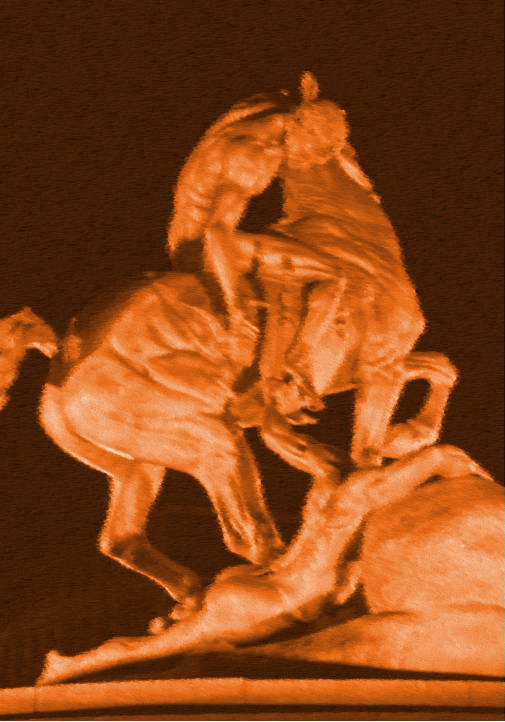
\includegraphics[width=\paperwidth]{Los_portadores_de_la_antorcha_-_05}}; % Background image
% Octavo
% \node[anchor=north west,inner sep=0pt] at (0,0) {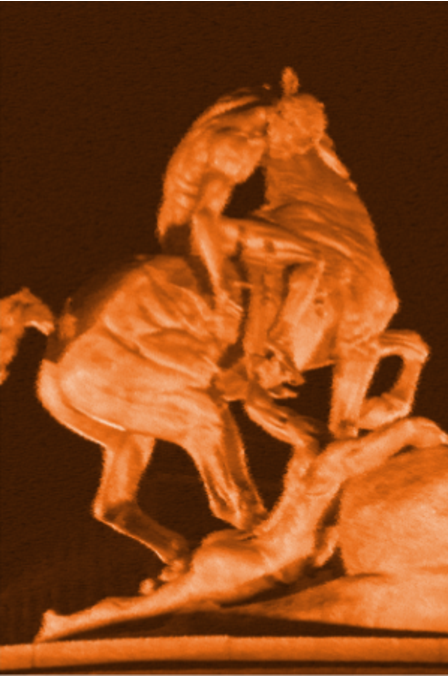
\includegraphics[width=\paperwidth]{Los_portadores_de_la_antorcha_Octavo}}; % Background image
% \node[anchor=north west,inner sep=0pt] at (0,0) {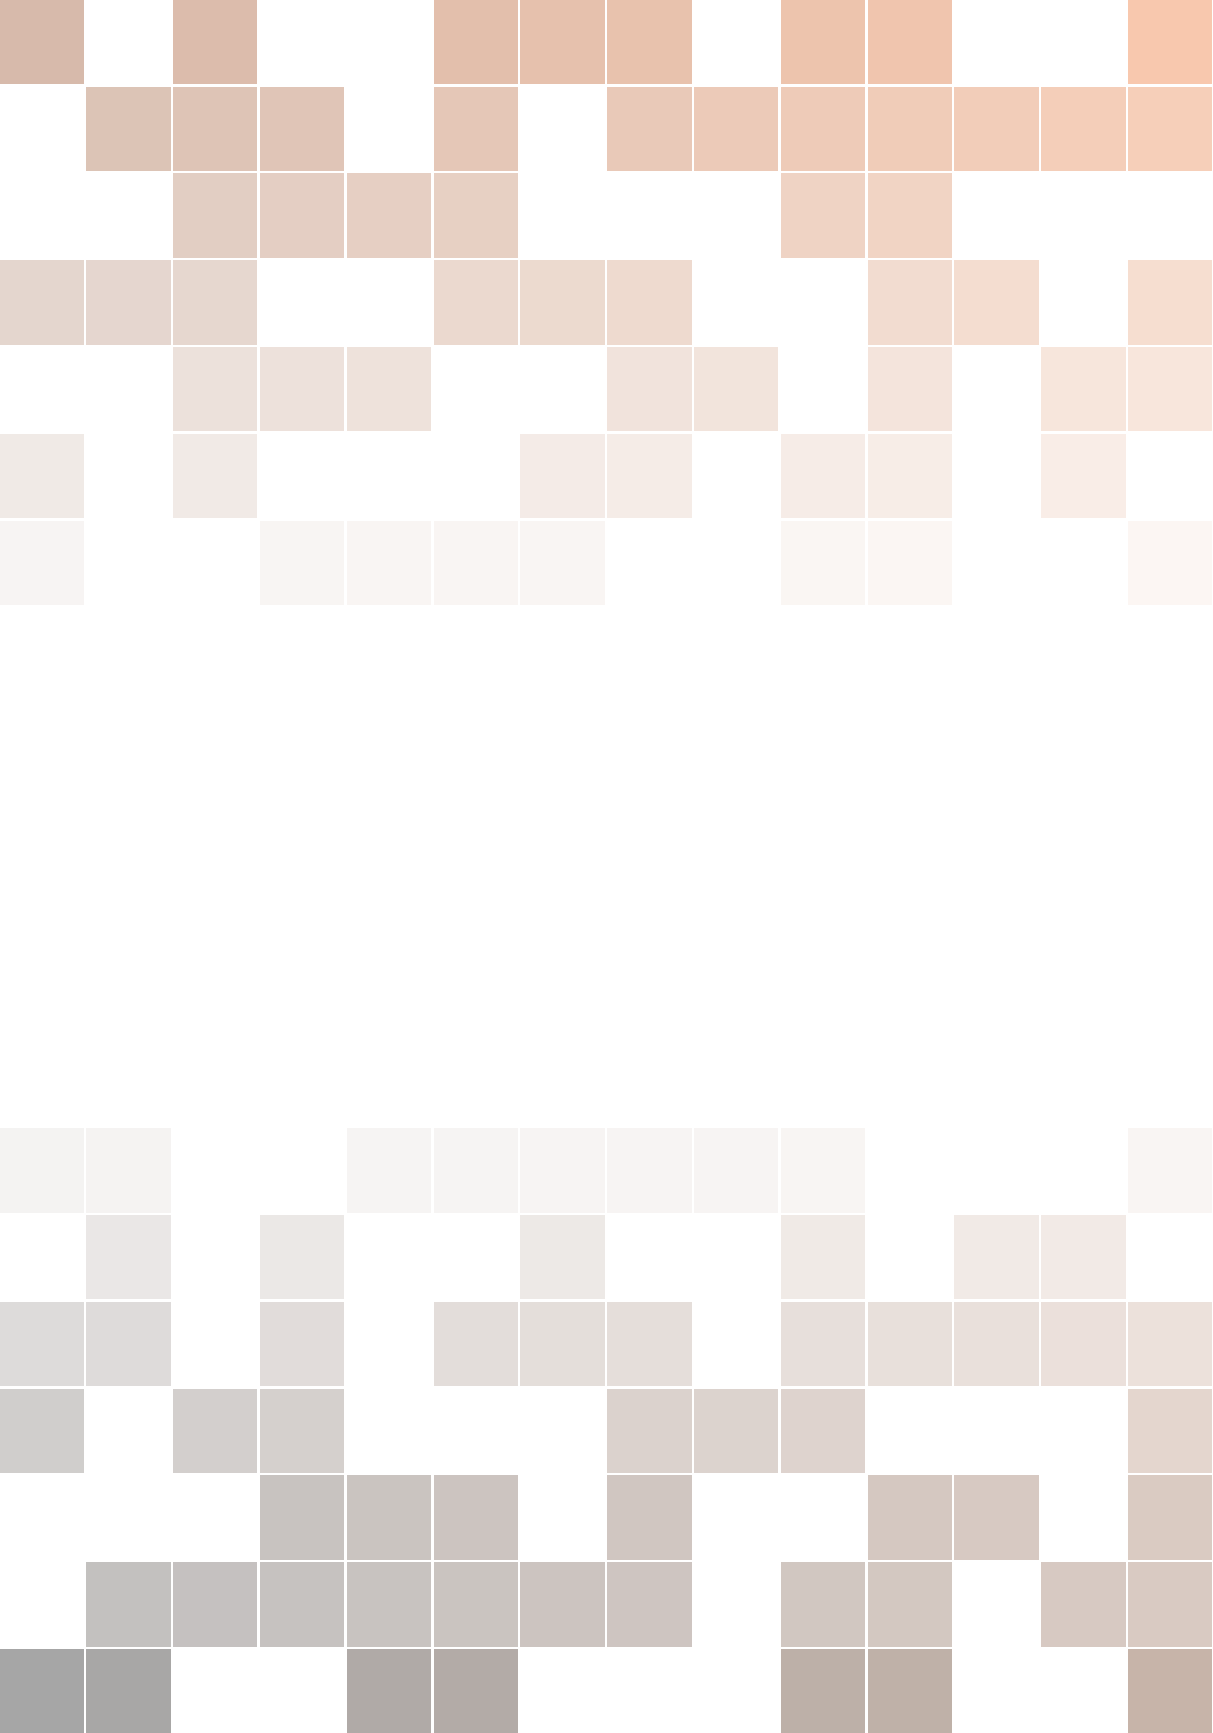
\includegraphics[width=\paperwidth]{background}}; % Background image
\draw[anchor=north] (midpoint) node [fill=ocre!30!white,fill opacity=0.6,text opacity=1,inner sep=1cm]{\LARGE\centering\bfseries\sffamily\parbox[c][][t]{\paperwidth}{\centering The Mathematics of the Unknown\\ % Book title
{\large Bringing to the present the knowledge of the future}\\[15pt] % Book subtitle
{\Large R. A. García Leiva}\\[15pt] % Author name
{\large (This book is 76\% complete)} % Disclaimer
}}; 
\end{tikzpicture}};
\end{tikzpicture}
\vfill
\endgroup

%----------------------------------------------------------------------------------------
%	COPYRIGHT PAGE
%----------------------------------------------------------------------------------------

\newpage
~\vfill
\thispagestyle{empty}

\noindent Copyright \copyright\ 2022 R. A. García Leiva % Copyright notice

\noindent www.mathematicsunknonw.com \\

\noindent \textsc{Published by the Author}\\ % Publisher


%------------------------------------------------------------------------------
%    CITA
%------------------------------------------------------------------------------

% Inserta una página en blanco
\newpage\null\thispagestyle{empty}\newpage

\newpage
\thispagestyle{empty}

\begin{quote}
\begin{flushright}
This book is dedicated to my wife Justi, \\
my son Daniel, and my two daughters Teresa and Lucía.
\end{flushright}
\end{quote}


%----------------------------------------------------------------------------------------
%	TABLE OF CONTENTS
%----------------------------------------------------------------------------------------

\chapterimage{Philosophers.pdf} % Table of contents heading image

\pagestyle{empty} % No headers

\tableofcontents % Print the table of contents itself

% \listoffigures

% \listoftables

\cleardoublepage % Forces the first chapter to start on an odd page so it's on the right

\pagestyle{fancy} % Print headers again

%
% Preface
%

%
% Preface
%

\chapterimage{Ramon_Llull_-_Ars_Magna_Fig_1.pdf} % Chapter heading image

\chapter*{Preface}

\begin{quote}
\begin{flushright}
\emph{Perfection is achieved not when there is nothing more to add, \\
but when there is nothing left to take away.}\\
Antoine de Saint-Exupéry\\
\end{flushright}
\end{quote}
\bigskip

% An explanation of the main assumption behind the book

The main idea of this book is that perfect knowledge implies randomness. This is, in principle, a highly counterintuitive idea, since a lot of effort in science deals with the task to name, organize and classify our messy, chaotic, world. Even the kind of knowledge that explains how things work requires a previous ordering and classification. Science, apparently, is anything but random. Yet, this is not the case.

If it requires a lot of time to explain how something works, probably we do not fully understand it. For example, consider the calculus of derivatives. At its origin, during the time of Newton and Leibniz, it was required a lot of space to define the concept of limit of a function. Moreover, only the specialists, if any, were able to understand the idea. We had a highly incomplete knowledge. Today, the definition of derivative barely takes one paragraph in a math book, and it is taught at high school. Our current knowledge is much better. Long explanations are usually superfluous, they contain repeated ideas, unused concepts, improperly identified relations, bad notation, and so on. With a better understanding, normally after considerable research, we should be able to remove those unnecessary elements. And when there is nothing left to take away, we say that we have achieved a perfect knowledge. Hence, if a theory is perfect, that is, it presents no redundant elements we can remove, it description must be an incompressible string. And that is exactly the mathematical definition of random string, an incompressible sequence of symbols. In this sense, a scientific theory is random if it contains the maximum amount of information in the less space possible.

In this book it is described the new \emph{Theory of Nescience}, a mathematical theory that address the problem of what science is and how scientific knowledge is acquired. Our main assumption is that it is easier to measure how much we do not know than measuring how much we do know, because randomness posses a limit to how much we can know. A second assumption is that the computer, as a conceptual model, is the right tool to provide this quantitative measure.

The fact that randomness imposes a limit on how much we can know about a particular research topic, far from being a handicap, opens new opportunities in science and technology. The proper understanding of this limit will allow us not only to solve the most challenging open problems, but also to discover new interesting research questions. In the book I also describe some of the practical applications of the theory of nescience to the areas of scientific research, artificial intelligence, computational creativity and software engineering.

%
% Section: Research Agenda
%

\subsection*{Research Agenda}

The theory of nescience has been developed with the aim to provide answers to the following questions:

\emph{Q1: Can we provide a quantitative characterization of how much we do not know about a research topic?} Given this metric we could not only measure how much we do not know about a particular topic, for example climate change, but also we could measure how much a new development or idea (usually published in the form of a research paper) contributes to increase our knowledge. If we combine this metric with a measure of the relevance of the problem investigated, we could quantify the value of new scientific contributions.

\emph{Q2: Is it possible to compare how much we do not know about topics from unrelated scientific areas?} If so, we could classify and compare all the open questions according to how much we do not know about them, regardless of the disciplines to which they belong (physics, biology, sociology, etc.). This classification, together with the already mentioned metric of relevance, will allow us to decide where we should concentrate our research efforts. I am not proposing to stop doing research in basic or fundamental science, on the contrary, I will show we need this kind of science. The goal is is to identify, and possibly cancel, nonsense or useless research.

\emph{Q3: How can we distinguish between science and pseudo-science?} This is a long standing, still open, question in philosophy of science. It would be very nice to have a mathematical answer that can be implemented in practice, since that would allow us to assess how scientific are some controversial disciplines that call themselves science.

\emph{Q4: Are some research topics inherently more difficult to understand than others?} So we could elucidate if this true that researchers of some disciplines (e.g. physics) are smarter than researchers of other disciplines (e.g. sociology) as they claim, or it is just a matter that the former are far easier to understand than the laters.

\emph{Q5: Are there topics beyond the capabilities of human comprehension?} What are the limits of human understanding? Maybe there exists problems that can not be solved by humans, and research topics that our limited brain can not comprehend. Perhaps we should get used to that progress, in certain research areas, can be only achieved if we give-up and let computers do the creative scientific work.

\emph{Q6: Is there a systematic procedure to increase our knowledge?} It might happen that what we call the "scientific method" is in fact a non-solvable problem, and the only thing we can provide is a practical approximation. And, if this is the case, how do we evaluate and compare different approximations? Can we provide a new and better method based on the principles of the theory of nescience?

\emph{Q7: What is the effort required to fully understand an unknown topic?} For example, how much does it cost to increase by 1\% our understanding of how to cure cancer? Given this  metric we could plan our research activities according to priorities, budget, and relevance of potential results. Of course, this metric would be a lower bound, since we could still do it much worse, for example, due to bad project management.

\emph{Q8: What is perfect knowledge? Can perfect knowledge be achieved for all possible entities?} Randomness is a necessary condition for perfect knowledge, but we need something more to characterize what full understanding means. Moreover, we have to prove if perfect knowledge is always achievable or, on the contrary, there are fundamental limitations that make perfection in science a chimera. 

\emph{Q9: Is there a procedure to discover new, previously unknown, interesting research entities and problems?} We need a method to explore the unknown unknown, that is, those problems that not only we do not know how to solve, but also, we are not even aware they exists. Such a method would allow us to bring to the present the research topics of the future.

Some of the answers provided in this book are more mature than others. For some questions I will provide a full theoretical answer with a practical implementation, and for others, just a rough sketch of what a solution could be. But I am firmly convinced that with more research, the new theory of nescience can provide satisfactory answers to all the posed questions. In this sense, this book is more a research agenda than a comprehensive description of a full theory of nescience.

%
% Section: Origins of the Theory of Nescience
%

\subsection*{Origins of the Theory of Nescience}

I think it was in 1991 (when I was eighteen) that I read for the first time the sentence \emph{"Computers are useless, they can only give you answers"}. The quote is attributed to Pablo Picasso, one of the most creative and influential artists of the 20th century. Soon I realized how terrible right he was, since it is true that computers cannot make interesting, original, questions. But it was more than 20 years later, in 2014, when I started to look seriously to the challenge that Picasso posed to the computer science community.

Most of the concepts behind my methodology for the discovery of interesting questions were formulated in just one night that I could not sleep: nescience, relevance, unknown unknown, and many others. Or perhaps they were developed by my subconscious mind during all those 20 years, since I do not think it was a matter of luck that I decided to pursue subjects like information theory or Kolmogorov complexity long before I was aware that they were the foundation of a future theory of nescience. What it is remarkable is that it took me just one single night to come up with a rough sketch of the most important ideas, a couple of months to develop the initial computer experiments that validated them, and several years to fully develop the mathematics needed to provide the theoretical support.

At the beginning, I was mostly interested in finding interesting scientific questions, that is, to discover what it is hidden in what I call the unknown unknown area, with the aim of bringing to the present the research topics of the future. Later on I started to look into the evolution of the nescience of scientific topics over time, and I asked myself what would happen if we keep improving a theory forever. It is then when I realized that perfect knowledge implies randomness, and the original methodology for the discovery of interesting questions was extended into a full theory of nescience to develop this important idea.

I may confess that the new theory has had, in general, a pleasant welcome form my colleges and those scientists to whom I had the opportunity to talk during the initial development stages. This early success encouraged me to continue with a further improvement of the main ideas and their applications in practice. Meanwhile I was developing the mathematics supporting the concept of nescience, I started to look into other potential applications, including the analysis of computer programs (quality assurance) and raw datasets (machine learning).

However, I was not satisfied with the status of the theory in spite of its explanatory power. It is true that given the theory I was able to provide solutions to some open questions in the area of philosophy of science, for example, how well we understand mathematics compared to sociology, why some research topics are more difficult that others, what it is the fundamental difference between science and pseudoscience, and many others. But the problem was that the theory did not provide any predictions that could be falsified by means of running an experiment. So I decided to take the risk and further develop the mathematics to provide such kind of predictions. This is when I came up with the function that describes how nescience decreases as we increase our research effort. This function allows us to predict the maximum increment of knowledge that we can gather about a topic given the amount of effort we are willing to put in its understanding. But, still not fully satisfied, I decided to push the theory one step forward and try to find a novel prediction, that is, something that had not been observed before. New developments of the mathematical foundations behind the theory allowed me to discover the highly counterintuitive property that sometimes, for a certain class of topics, further research could be a counterproductive activity. That is, that more research we do, the more confused we get, since for these topics it is not possible to increase our knowledge beyond a critical point, even if this point if far from a perfect knowledge.

%
% Section: About the book
%

\subsubsection*{About the Book}

{\color{red} Update once the book is finished.}

The theory of nescience borrows concepts from multiple academic disciplines: computability, randomness, information theory, complexity, probability, graph theory, philosophy of science, and many more. However, the book is self-contained, and so, no previous knowledge is required to follow the mathematical developments, beyond familiarity with first year calculus, abstract algebra and some computer programming experience. The contents have been selected to cover the needs of readers with very different backgrounds: mathematicians, computer scientists, engineers, ... The math level is that of a graduate student or advanced undergraduate.

The book has been structured into three main parts: Background, Foundations and Applications. Readers already familiar with the mathematics covered by the Background section can directly proceed to the Foundations part. However, it is highly recommended to perform at least a quick review of the notation used in these chapters. After getting acquainted with the details of the theory of nescience described in the Foundations section, the reader can continue with the applications. It is not necessary to fully understand all the details of the theory in order to follow the applications. A basic knowledge of the main concepts and results should be sufficient.

\bigskip

\begin{itemize}

\item \emph{Chapter \ref{chap:Introduction} Introduction} contains a gentle introduction to the theory of nescience, and a short review of the main results. The chapter avoids the use of advanced mathematics, but the concepts are still semi-formally introduced. Although it is not recommended, those readers that cannot follow the mathematics behind the theory could just read this first chapter, the introductory sections of the remaining chapters of the Background and Foundations parts, and then proceed directly to the applications.

\end{itemize}

\bigskip

\emph{PART I Background} is an introduction to the mathematics required to measure how much we do not know about a topic and how random is a string. The goal of this part is to fix notation, formally define concepts, and prove some important results. I do not assume any previous knowledge to follow the covered material, however, to fully understand these topics I recommend to refer to the standard literature (see the References section included at the end of each chapter).

\begin{itemize}

\item \emph{Chapter \ref{chap:Discrete_Mathematics} Discrete Mathematics} is an overview of the basic mathematics required to understand the more advanced topics covered in the book. This chapter is intended as a quick review of these concepts, and so, no formal definitions are provided and theorems are not proved. Among others, the topics covered include sets, relations, strings, graphs and discrete probability.

\item \emph{Chapter \ref{chap:Computability} Computability} provides a formal definition of the concept of algorithm. We will introduce the concept of universal Turing machine, and we will see that there are well defined mathematical problems that cannot be solved by computers. The very important tools of oracle Turing machine and Turing reducibility are also studied in detail. Computational complexity main results are briefly reviewed.

\item In \emph{Chapter \ref{chap:Coding} Coding} we will study the properties of codes, and in particular, how codes allow us to compress a text without loosing any information by means of removing statistical redundancy. We will see that there exists a limit to how much a text can be compressed by using this technique, and that this limit is given by the entropy of the source.

\item \emph{Chapter \ref{chap:Algorithmic_Information} Complexity} introduces an absolute metric, called Kolmogorov complexity, to measure the amount of information contained in a string, by computing the length of the shortest computer program that can print that string. The properties of this metric are studied in detail. The relation between string complexity and randomness is also discussed.

\item \emph{Chapter \ref{ch:Learning} Learning} studies the relation between codes and probabilities. It provides a short review of the area of statistical learning, with a focus on existing approaches that apply the concept of minimum string length to the problem of stochastic models evaluation and optimal parameters selection. An introduction to the concepts and notation of nonlinear multiobjective optimization problems is included as well. 

\item \emph{Chapter \ref{chap:Philosophy} } is a short introduction to the discipline of philosophy of science. We will review concepts like scientific representations, models, theories and many other components of science from a philosophical point of view, identifying the most important elements that any formal theory of science should include. The chapter also contains a review of the current state of the art of what it is the scientific method.

\end{itemize}

\bigskip

\emph{PART II Foundations} contains a detailed description of the theory of nescience, defining formally the concepts involved and proving the main theoretical results. This is the most important part of the book, where the new theory is fully developed. Readers with a solid background in computability, complexity, information theory and statistics could proceed directly to this part.

\begin{itemize}

\item \emph{Chapter \ref{cha:Topics-and-Descriptions} Representations} introduces the basic constituents of the theory of nescience: entities, representations and descriptions. The properties of these elements and how they interlace together are studied. We will see how multiple representations and descriptions can be combined, and how to include background knowledge in a research. The relation between perfect knowledge and randomness is discussed, and a novel concept of research area is proposed.

\item \emph{Chapter \ref{chap:Miscoding} Miscoding} address the difficult problem of how to represent abstract, and non-abstract, research entities as string of symbols that can be used for research. In the chapter we will formally introduce the concept of miscoding and study its properties. Miscoding is a quantity that measures the error introduced due to improper encodings.

\item \emph{Chapter \ref{chap:Error} Inaccuracy} contains a novel interpretation of the classical concept of error, that is, how accurately a description explains an entity. The concept of inaccuracy is extended to deal with all kinds of topics, including abstract ones. The joint and conditional versions of the concept of inaccuracy are introduced and their properties studied.

\item \emph{Chapter \ref{chap:Redundancy} Surfeit} studies how redundant is a description, that is, how many unnecessary elements a description contains. Surfeit can be seen as a measure of how well we currently understand research topics and research areas. The joint and conditional versions of surfeit are provided as well.

\item \emph{Chapter \ref{chap:Nescience} Nescience} is the central chapter of the book, since it contains the mathematical foundations of the new theory. In the chapter is formally defined the concept of nescience and its main properties studied, like for example, how nescience evolves with time, what we mean by perfect knowledge, and how to identified our current best model.

\item \emph{Chapter \ref{chap:scientific-method} Scientific Method} introduces the mathematical details of one of the most important applications of the theory of nescience, a novel computational approach to discover new knowledge, and solve open problems (scientific method), based on creative combination of already known entities, and the automated discovery of new ones.

\item \emph{Chapter \ref{chap:Interesting-Research-Questions} Interesting Questions} describes a procedure to find new interesting things in a large collection of measurable objects, and in particular, to find new interesting research questions and new research topics. New concepts like relevance and applicability are defined and studied.

\item \emph{Chapter \ref{chap:Properties-Nescience} Advanced Properties} covers some advanced concepts and properties of the theory of nescience. These properties are not needed to understand the applications of the theory, and so, they can be safely skipped in a first read of the book (but, definitely, not in a second). Among others, new concepts introduced include: an axiomatic version of the theory, graspness as a measure of how difficult is a particular research topic, or the minimum effort required to reduce the nescience of a topic.

\end{itemize}

\bigskip

\emph{PART III Applications} provides a collection of practical applications of the concept of nescience, in the areas of machine learning, software engineering, philosophy of science, and computational creativity. The applications have been selected to cover the entire spectrum of possible kinds of topics, from abstract ones (research topics), real objects and strings (computer programs).

\begin{itemize}

\item \emph{Chapter \ref{chap:Machine-Learning} Machine Learning} describes how the concept of nescience can be applied in the case of entities represented by large datasets. In particular, the methodology will be applied to select relevant features, identify optimal models, and compute errors. Some new machine learning algorithms, like a novel approach to derive optimal decision trees, will be proposed as well.

\item \emph{Chapter \ref{chap:Software-Engineering} Software Engineering} covers how to use the theory of nescience with computer programs, in order to provide a measure of how well we understand current software platforms (operating systems, networking middleware, productivity tools, ...). We will evaluate if current versions of software are better than past versions, or if software is degrading with time. The results are also applied to the automatic discovery of errors, with the aim to improve the quality of software.

\item \emph{Chapter \ref{chap:philosophy-science} Philosophy of Science} studies how to apply the new metrics introduced in this book to study of what it is science and how science is made. Some important open problems in the area of philosophy of science will be addressed, including the demarcation problem (how to distinguish between science from pseudoscience) and the question of how science make progress. Multiple proposals of what it is the scientific method are evaluated in the context of the theory of nescience, and compared against our own proposal.

\item \emph{Chapter \ref{chap:computational-creativity} Computational Creativity} shows how to apply in practice the methodology for the discovery of interesting things. In particular, the methodology will be applied to find new research questions and new research topics, where multiple examples of interesting questions and topics will be provided.

\end{itemize}

\bigskip

\emph{Appendix \ref{apx:math} Advanced Mathematics} contains a brief description of some mathematical concepts that have been used in the book, but that play a secondary role in the development of the theory; they are included in this appendix for reference.

Last, but not least, \emph{Appendix \ref{apx:photos} About the Photos} explains the origin and intended meaning of the carefully selected photographs included at the header of each chapter.

%
% Section: Acknowledgements
%

\section*{Acknowledgements}

I would like to give thanks to all the people who has contributed with comments and ideas to the development of the theory of nescience. In particular, I would like to give thanks to Antonio Fernández, Vincenzo Mancuso and Paolo Casari who believed and supported this project since its very beginning, when it was only a crazy nonsense idea (although perhaps it still is). Other people who has provided contributions and useful comments where Héctor Cordobés, Luis F. Chiroque, Agustín Santos, Marco Ajmone, Manuel Cebrián, Andrés Ortega, Emilio Amaya, Mattis Choummanivong, Alexander Lynch, Andrés Carrillo and Simon Bihoreau. The \texttt{fastautoml} library described in Chapter \ref{chap:Machine-Learning} has been partially funded by the IMDEA Networks Institute and the European Union's Horizon 2020 research and innovation programme under grant agreement No 732667 RECAP.

Finally, I would like to give thanks to my parents who gave me the opportunities in life they didn't have, and to my wife and my three kids who provide ultimate meaning to my life.

%
% Section: Disclaimer
%

\section*{Disclaimer}

I would like to leave it clear that the overwhelming majority of the ideas contained in this book are not mine. The intuition comes form the great minds of our history: Occam, Llull, Leibniz, Newton, etc., and from philosophers like Plato, Popper, Feyerabend, Wittgenstein, etc. Also, I have leveraged on the mathematical theories developed by scientists like Turing, Church, Post, Shannon, Solomonof, Chaitin, Kolmogorov, and many others. My only original contribution with this book is that I have, perhaps, connected some dots, and that I have provided a, perhaps, interesting reinterpretation of some old ideas. In the References sections included at the end of each chapter there is a description of the works I have used to write the book. In the text I use passive voice ("it is defined") whenever I know that a concept is not mine, and active voice ("we define") when I am not aware of a previous use of this concept by somebody else.



%
% CHAPTER: Introduction
%

%
% Introduction
%

\chapterimage{Galileos-telescope-002.pdf} % Chapter heading image

\chapter{Introduction}
\label{chap:Introduction}

\begin{quote}
\begin{flushright}
\emph{If presented with a choice between indifferent alternatives,\\
then one ought to select the simplest one.}\\
Occam’s razor principle 
\end{flushright}
\end{quote}
\bigskip

The quest for knowledge usually starts by identifying a set of entities we would like to understand. The elements of this set can be almost anything. If we are mathematicians, our set of interest will be composed by mathematical concepts; if we are biologists, the set will be living things; and if we are engineers, it will be machines that solve problems. Our goal, as researchers, is to understand as much as possible about those entities. We want to understand how things work because that allows us to forecast the consequences of our actions. For example, we know that if we apply a sufficient amount of heat to a pile of wood, a fire will start. Also, and more challenging, looking at consequences we can try to infer the causes; if I have fever, maybe I have been infected by a virus. Understanding is how we solve problems in practice, and understanding means to find patterns or regularities that allows us to build a simplified description, or model, of the original entities so we can manipulate them to our convenience.

Ideally, we would like that given our descriptions we should be able to reconstruct the original entities under study. However, for the majority of entities this is not possible, like for example with the abstract ones. Instead, what we have to do is to work with representations, that is, use texts or data that try to capture as many details of the original entities as possible. If we are physicists the representation of an entity could be the result of an experiment, if we are computer scientists it could be a dataset composed by measurements, or if we are sociologists what we might have is a collection of observed facts. In Figure \ref{fig:representationProblem} it is depicted this process: we would like our descriptions to model entities, but what they model is our artificial representation of those entities.

\begin{figure}[h]
\centering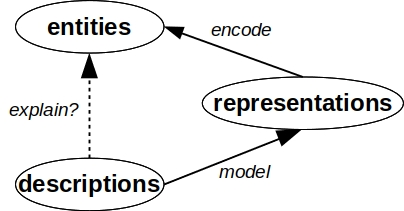
\includegraphics[scale=0.5]{representationProblem}
\caption{\label{fig:representationProblem}The Problem of Understanding.}
\end{figure}

The question is how well our descriptions explain the original entities through the modeling of the representations that encode those entities. There are multiple sources of error we should consider. The first one is that our encoding method might not be perfect. That is, if the ideal representation of an entity $e$ is the string $r$, in practice we could be working with another string $r'$ that it is close to $r$, but not equal. We call this type of error \emph{miscoding}\index{Miscoding}. The second source of error is due to the fact that our descriptions are not perfect. Ideally a description $d$ should allow us to recreate the string $r'$ (the string $r$ is normally unknown), but in practice it produces another string $r''$ which is, again, close to $r'$ but not equal. This second type of error is what we call \emph{inaccuracy}\index{Inaccuracy}. Finally, the third group of errors deals with the descriptions themselves. Given the limited cognitive capabilities of humans, we are interested in the shortest possible description $d$ of $e$, so we can understand the entity, make predictions, or derive consequences. However, our current best known description $d'$ probably will be longer than $d$. This third type of error is what we call \emph{surfeit}\index{Surfeit}. Finally, we combine these three types of errors, miscoding, inaccuracy and surfeit, in a single quantity called \emph{nescience}\index{Nescience}, as a quantitative measure of how much we do not know about an entity.

This chapter contains a gentle introduction to our new \emph{theory of nescience}, and a short review of the main results of this theory. The chapter avoids the use of advanced mathematics, but concepts are still semi-formally described. Also, in order to clarify the new ideas introduced, we provide multiple practical examples.

%
% Section: Entities
%

\section{Entities}

Our theory starts by assuming there exists a non-empty collection of \emph{entities}\index{Entity}, denoted by $\mathcal{E}$, that are the subject of past, present or future scientific research. And, of course, we assume that (at least some of) these entities can be fully understood and described by science. Technically speaking $\mathcal{E}$ is not a well defined set, since the only restriction is that it must be nonempty. The abstract nature of $\mathcal{E}$ has some advantages, but also introduces important limitations. The main limitation is that our definition of nescience is, in general, a non-computable quantity, and so, it must be approximated in practice. The main advantage is that we can apply the new concepts and methods introduced in this book to other domains, not only to the discovery of solutions to open problems.

In the theory of nescience we do not allow universal sets, that is, we cannot assume the existence of a set $\mathcal{E}$ that contains everything. The problem of universal sets is that they violate Cantor's theorem\index{Cantor's theorem} (see Section \ref{sec:descriptions_entities}). Cantor's theorem states that the set $\mathcal{P}(\mathcal{E})$ composed by all the possible subsets of $\mathcal{E}$ has more elements than the original set $\mathcal{E}$, and this is a contradiction with the fact that $\mathcal{E}$ contains everything. In the theory of nescience $\mathcal{E}$ must be the set of "something". Moreover, not all possible sets are allowed. For example, the Russel's paradox\index{Russel's paradox} propose to consider the set $\mathcal{E}$ composed by all those sets that are not members of themselves; the paradox arises when we try to answer the question of whether $\mathcal{E}$ is a member of itself or not (see Section \ref{sec:descriptions_entities}). We require from every set $\mathcal{E}$ to be restricted to one particular type of elements, so they cannot be members of themselves.

Usually the set $\mathcal{E}$ corresponds to an individual domain of knowledge, and its constituent elements depend on how the theory is being applied in practice. Examples of such sets of entities could be: a collection of mathematical objects (abstract); the kingdom of animalia (living things); known and unknown human needs (abstract); all possible computer programs (strings of symbols), etc.

%
% Section: Representations
%

\section{Representations}

Most of the entities can not be the subject of a direct scientific analysis because, for example, they are abstract objects. Instead, what we have to do is to work with representations of those entities. Let $\mathcal{R_\mathcal{E}}$ be the collection of finite binary strings, called \emph{representations}\index{Representation}, that encode the entities of $\mathcal{E}$. The exact format of these strings is something that depends on the entities in which the theory of nescience is being applied. In some cases, entities will be strings themselves (e.g. computer programs), and in others they will be abstract objects that have to be encoded as strings (e.g. human needs). Note that an entity $e \in \mathcal{E}$ might have more than one valid representation in $\mathcal{R_\mathcal{E}}$. How to encode abstract entities as strings of symbols in such a way that they capture all the details and nuances of the original entities is a difficult, still unsolved, problem, and so, the set $\mathcal{R_\mathcal{E}}$ is normally unknown. 

Ideally, we would like to have an encoding function $f:\mathcal{E} \rightarrow \mathcal{R_\mathcal{E}}$ from a set of entities $\mathcal{E}$ to the set of all possible representations. Unfortunately, in practice, it is not possible to define such a function, since as we have already mentioned, the set $\mathcal{E}$ is not a well defined set, that is, we cannot tell what it is and what is not a member of this set. For example, it requires a lot more research before we can tell exactly what a human need is.

From a theoretical point of view we could take advantage of the concept of \emph{oracle Turing machine}\index{Oracle Turing machine} (see Chapter \ref{chap:Computability}) to address this problem. A Turing machine\index{Turing machine} is a mathematical model of a computer, and an oracle Turing machine is somehow like a mathematical model of a computer connected to Internet. We could assume that this computer can query an hypothetical external service, hosted somewhere in another computer, to check if a given string $r$ encodes \emph{any} entity of $\mathcal{E}$. We cannot ask the oracle if the string $r$ is a valid representation of the entity $e$ in which we are interested, because that would require to provide a valid representation of $e$ as a string of symbols, something that we cannot do since, in general, it is unknown. The concept of oracle machine allow us to define a function from the collection of finite binary strings to the set of entities $f:\mathcal{B}^\ast \rightarrow \mathcal{E}$.

From a practical point of view, we usually approximate the set $\mathcal{R}_\mathcal{E}$ by another set $\mathcal{R} \subseteq \mathcal{B}^\ast$ of strings that we believe are good enough representations of the entities of $\mathcal{E}$. In science, traditionally, these representations have had the form of images or drawings (e.g. biology), collection of facts (e.g. sociology), or the result of experiments (e.g. physics). Recently, and due to the huge advances in the capacity of computers to collect and store data, a new and powerful way to encode entities has emerged: the use of large collections of data as representations. Please mind that in the process of encoding we are not interested in finding the shortest possible representation of the entities, what we need is high quality representations.

We should be aware that in many practical problems, the selected representations of abstract entities will not be able to fully capture all the details of the original objects. That is, we are dealing with simplified abstractions of reality that might limit our capability of making universal statements about nature (see Chapter \ref{chap:Miscoding}).

\begin{example}
\label{ex:animals_DNA}
When the topics under study are animals (the set $\mathcal{E}$), we could use as representations a binary encoding of their DNAs (the set $\mathcal{R_\mathcal{E}}$). Although today we do not have the technology to grow a creature given its DNA, in theory it could be possible to do so. However, the DNA is not enough to fully reconstruct the original animal, since we also need to know what happened along its life. For example, what if we are dealing with a cat with only three legs because it lost one in an accident? That information is not included in its DNA. If we are interested in studying the characteristics of some species, it will be sufficient to work with the DNA of some representative sample of individuals that belongs to each species. However, if we are studying the particular individuals inside a species, we also need a way to encode the history of each animal, or a way to encode the details not covered by the DNA.
\end{example}

\begin{figure}[h]
\centering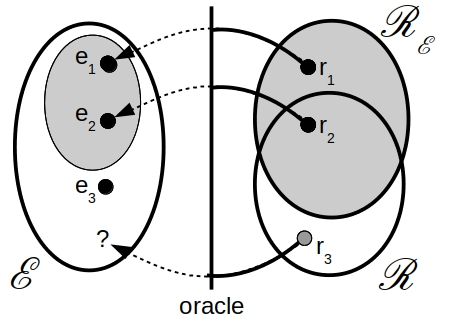
\includegraphics[scale=0.5]{entities_topics}
\caption{\label{fig:entities_topics}Entities and Representations.}
\end{figure}

A consequence of working with strings as representations (the set $\mathcal{R}_\mathcal{E}$) is that it might happen that there exist entities that are not encoded by any representation (see the gray areas in Figure \ref{fig:entities_topics}, in particular, the entity $e_3$ is not encoded by any representation). For example, if our set of entities is the set of real numbers, it turns out that there exist numbers that do not have a finite representation (we do not allow infinite strings as representations). Intuitively, we could say that for many domains of knowledge the number of problems is greater than the number of solutions. A consequence of working with approximations of representations (the set $\mathcal{R}$) is that some representations might encode the wrong entities (the representation $r_3$ in Figure \ref{fig:entities_topics}). This is due to the fact that our knowledge is incomplete, and we might be using incorrect representations for the entities of $\mathcal{E}$. Working with incomplete knowledge has an additional problem, there may be some entities whose existence we do not know yet, what we call the \emph{unknown unknown}\index{Unknown unknown}. For example, the representation $r_1$ in Figure \ref{fig:entities_topics} is not part of the set $\mathcal{R}$, and so, it is not currently considered by researchers even though it represents a valid entity $e_1$. We are interested in investigating a procedure to discover new, previously unknown, research entities from the set $\mathcal{R}_\mathcal{E}$ (see Section \ref{sec:intro_research_topics} and Chapter \ref{chap:Interesting-Research-Questions}).

A \emph{research area} $A$ is subset of topics, that is $A \subset \mathcal{R}_\mathcal{E}$. In practice, areas are useful as long as the topics included in the area share a common property. We might be interested in studying what we do not know about a particular area. For example, if the set of topics is "animals", examples of areas could be "invertebrates", "mammals", "birds", "amphibians", "reptiles" and "fish". In order to measure what we do not know about an area, first we have to provide a description of the topics included in that area. However, in general, our knowledge about the topics that compose an area is limited, and so, we can only partially describe them. Moreover, as our understanding of a research area changes, the number of topics included in its known subset changes as well. Consequently, the properties of areas can be studied only relative to our current knowledge.

\begin{example}
If our set of topics is "astronomy", a research area could be the set of "habitable planets", from which we currently known only a few of them. A model of this area would be a description of those already known habitable planets.
\end{example}

%
% Section: Descriptions
%

\section{Descriptions}

Once we have identified the set $\mathcal{R}$ of possible representations, we have to provide a way to describe them, that is, to formulate our theories or models about how things work. As humans, we have very limited cognitive capabilities, and so, we rely in the use of simple models of nature in order to understand observed facts, and to forecast the results of our own actions. 

What constitutes a valid description of an entity is a difficult, still unsolved, problem. For example, the Berry paradox\index{Berry paradox} proposes the following description "the smallest positive integer not describable in fewer than twelve words". The paradox arises because we have just described this number with only eleven words. In order to avoid these kind of paradoxes, in the theory of nescience we require that a description for an entity must be a finite string of symbols from which we can fully and effectively reconstruct one of the possible representations of the original entity. By "effectively reconstruct" we mean that our models must be computer programs that when executed they print the selected representation. Since Newton, science is about mathematical models, that is, the search of a set of functions that fully describe the objects found in Nature and their relations. In the theory of nescience we go one step beyond and require that those models must be computable.

Descriptions\index{Description} are composed by two parts, a Turing machine\index{Turing machine} $TM$ (a computer program) that implements all the regularities found in the entity's representation (the compressible part), and an input string $a$ to this program that contains a literal description of what is left (the non-compressible part). From a formal point of view, a description for a representation $r \in \mathcal{R}$ is a string $\langle TM, a \rangle$ such that $TM(a) = r$. This two part nature of descriptions somehow resembles our classical distinction between theories and assumptions, theories and initial conditions, problems and particular instances of problems, species and individuals, etc. For example, a description could be composed by a set of differential equations modeling a system (the compressible part), and the collection of initial conditions (the non-compressible part). The actual interpretation of the pair $\langle TM, a \rangle$ is something that depends on the particular details of the set of entities in which that theory is being applied.

\begin{figure}[h]
\centering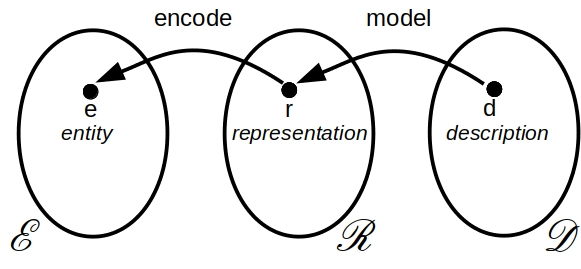
\includegraphics[scale=0.5]{entities_topics_models}
\caption{\label{fig:entities_topics_models}Entities, representations and descriptions.}
\end{figure}

In Figure \ref{fig:entities_topics_models} it is shown graphically the relation between entities, representations and descriptions (the set of all possible descriptions is denoted by $\mathcal{D}$). Not every possible string is a description, since we require that a descriptions must be based on Turing machines, and not all possible descriptions describe valid representations.

\begin{example}
From an intuitive point of view, if we are studying how our world works, from a physical macroscopic point of view, our set of possible descriptions would include, among others, the following elements: Aristotelian physics, Cartesian physics, Newtonian physics, Einstein's theory of general relativity and superstring theory. Our current best description would be  Einstein's theory of general relativity (superstring theory has not been validated experimentally yet).
\end{example}

A representation $r \in \mathcal{R}$ can have multiple descriptions, and so, the goal of science is to find the shortest possible description, denoted by $d^\star$, that allows us to fully reconstruct the representation $r$. Unfortunately, there does not exist a method or algorithm that given a string, returns the shortest possible computer program that prints that string (see the result of incomputability of Kolmogorov complexity in Chapter \ref{chap:Algorithmic_Information}). In particular, there does not exist a method that given a representation finds the shortest possible description. That is, science is a non-computable problem and so, we have to find a collection of heuristics that allow us to approximate the optimal solution. This collection of heuristics is what we call a \emph{scientific method}\index{Scientific method}.

In the theory of nescience we are interested in understanding, and quantitatively measuring, what can be wrong in the ideal process depicted in Figure \ref{fig:entities_topics_models}. In Sections \ref{sec:ch1_miscoding}, \ref{sec:introduction:inaccuracy}, and \ref{sec:ch1_surfeit} we will propose a collection of metrics to measure each possible source of error, and in Section \ref{sec:ch1_nescience} we will see how to combine all these concepts into a single quantity, called \emph{nescience}. The new metric of nescience allow us to quantitatively measure how much we do not know about a research entity.

%
% Section: Miscoding
%

\section{Miscoding}
\label{sec:ch1_miscoding}

As we have seen, for the majority of the scientific disciplines, the set $\mathcal{E}$ of entities under consideration could be composed by abstract elements, or other kind of objects that are not easily represented as a string of symbols. Also, it might happen that our current understanding of the elements of $\mathcal{E}$ is limited, and so, we can not properly encode them. In those cases we have to work with approximate representations instead of the valid representations. We are interested in knowing the error introduced due to the use of these incorrect representations.

\begin{figure}[h]
\centering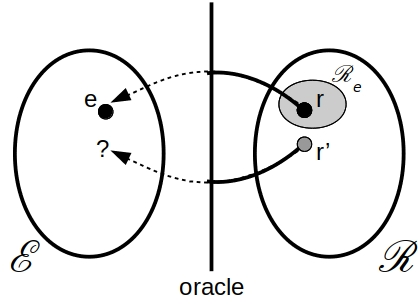
\includegraphics[scale=0.5]{miscoding}
\caption{\label{fig:miscoding}Miscoding of topics.}
\end{figure}

We propose to quantify the \emph{miscoding}\index{Miscoding} of an incorrect representation $r'$ as the length of the shortest computer program that can print the correct representation $r$ having as input $r'$, denoted by $K(r|r')$. See Figure \ref{fig:miscoding}, where $\mathcal{R}_e$ denotes the set of strings that correctly represent the entity $e$. Intuitively, miscoding measures the effort (measured as the length of a program, not as the time it takes to that program to do its work) required to fix the incorrect representation. For example, if our representation contains some errors, the program should be able to identify and correct those errors; or if our representation is missing some critical information required to fully encode the entity, the program will contain, hard-wired, that missing information.

However this approach is not sufficient to fully capture our intuitive notion of miscoding. The problem arises when our represenation $r'$ contains additional information that is not needed to encode the entity $e$. In this case, it might happen that our descriptions include elements modeling those unnecessary symbols, making them artificially long. For example, in a experiment we could be measuring features that do not influence at all the result of the experiment, and given our limited understanding of the original entity, our current description could include those features as predictors\footnote{\color{red} TODO: This example is confusing, since the experiment describes a cause-effect situation, and our machine learning algorithm could identify non-relevant features authomatically. Use a different example.}. In order to avoid this problem, we have to compute also the length of the shortest computer program that can print the incorrect description $r'$ having as input the correct one $r$, that is, $K(r'|r)$. Then, miscoding could be defined as the maximum of these two lengths $\max\{ K(r \mid r'), K(r' \mid r)\}$.

Unfortunately, this last definition still presents some practical problems. Most of the entities have multiple valid representations. Maybe $r'$ is far from a representation $r_1$, but it is closer to a second one $r_2$. It would be unfair to say that a description $d$ that perfectly model $r_2$ is a bad descriptions because it does not model $r_1$, since both, $r_1$ and $r_2$ represent the same entity $e$. A possible solution to this problem would be to look at $\min_{r \in \mathcal{R}_e} \{ \max\{ K(r \mid r'), K(r' \mid r)\} \}$.

\begin{example}
\label{ex:leibnez-wallis}
Let $e$ be the abstract entity called "Pi constant", that is, the ratio of a circle's circumference to its diameter; let $r$ be the Wallis' product\index{Wallis' product} $2 (\frac{2}{1} \cdot \frac{2}{3} \cdot \frac{4}{3} \cdot \frac{4}{5} \cdot \frac{6}{5} \cdot \ldots)$, one of the valid representations of $e$; and let $d$ be the description $\sum_{n=0}^\infty \frac{(-1)^n}{2n+1}$. It would be unfair to affirm that $d$ is a terribly bad description for the entity $e$ because it does not print $r$. In fact, $d$ produces the Leibniz's series\index{Leibniz's series} $4 (1 - \frac{1}{3} + \frac{1}{5} - \frac{1}{7} + \ldots)$ that it is also a valid representation of Pi. Leibniz's series should not be classified as a miscoded representation of Pi, even in the hypothetical case that it were unknown by mathematicians.
\end{example}

As example \ref{ex:leibnez-wallis} pointed it out, one of the most difficult problems with the definition of miscoding is that the set $\mathcal{R}_e$ of valid representations for the entity $e$ is, in general, not known. From a theoretical point of view we could resort again to the oracle Turing machine\index{Oracle Turing machine} to address this problem. However, as we have seen, we cannot ask the oracle if the string $r$ is a valid representation of the entity $e$ in which we are interested (the set $\mathcal{R}_e$), since that would require to provide a valid representation of $e$ as a string of symbols, something that, in general, cannot be done. The only thing we can do is to ask the oracle how far the string $r$ is from being a valid representation of any entity from the set of entities $\mathcal{R}_\mathcal{E}$.

Taking into account all the above considerations, we define the miscoding of a representation $r$, denoted by $\mu(r)$, as:
\[
\mu(r) = \overset{o}{ \underset{r_e \in \mathcal{R}_\mathcal{E}} \min} \frac{ \max\{ K(r_e \mid r), K(r \mid r_e) \} } { \max\{ K(r_e), K(r) \} }
\]
where $\overset{o} \min$ means that the minimum function has to be computed by an oracle. Note that in the definition we have introduced the normalization factor $K(r_e)$, that is, the length of the shortest program that can print $r_e$, because we are interested in comparing the miscoding of multiple, possibly unrelated, representations.

Since miscoding does not take as argument the original entity $e$, it may be the case that what we are representing is not what we were expecting. That is, with our representations and descriptions we might be studying a different entity. This is something that happens quite often in the practice of scientific research. 

\begin{example}
At the end of the eighteenth century, the chemist Joseph Priestley thought he was studying the nonexistent entity called "phlogiston"\index{Phlogiston}, a fire-like element that was supposed to be contained within combustible bodies and released during combustion. It turned out that he was studying a completely different entity called "oxygen".
\end{example}

According to the theory of nescience, our task as researchers is not only to find the proper representations of the entities of $\mathcal{E}$, but also to discover how this ideal oracle machine that knows how to properly encode entities works. That is, why our representations constitute good encodings of the entities under study.

%
% Section: Inaccuracy
%

\section{Inaccuracy}
\label{sec:introduction:inaccuracy}

In the previous section we have characterized how much we do not know about an entity $e$ in terms of the miscoding due to using a wrong representation $r'$ instead of a correct one $r$. In this section we are interested in how much we do not know given a description. Ideally we should be working with a description $d$ that allows us to fully reconstruct the representation $r'$ (recall that the representation $r$ might be unknown), but in general this is not the case in practice. Normally we will be working with a description $d'$ that prints out a string $r''$ (remember that we require that descriptions must be computer programs) that it is (hopefully) close to the string $r'$, but not equal. In this case we say that the description $d'$ is an \emph{inaccurate} description of the representation $r'$ (see Figure \ref{fig:inaccuracy:inaccuracy:inaccuracy}).

\begin{figure}[h]
\centering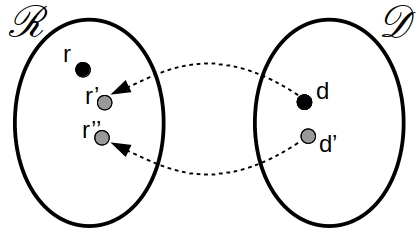
\includegraphics[scale=0.5]{inaccuracy}
\caption{\label{fig:inaccuracy:inaccuracy:inaccuracy}Inaccuracy of a description.}
\end{figure}

If a description is inaccurate for a representation, we would like to have a quantitative measure of how far we are from properly modeling the representation. A natural way to define this measure would be by means of computing the effort required to fix the output of our inaccurate description. In this sense, inaccuracy could be given by the length of the shortest computer program that can print the representation given as input the wrong representation produced by the description. However, as it was the case of miscoding, in order to have a complete picture of the error made with the description $d$ we have to compute also how difficult is to print the inaccurate representation given the good one. It might happen that our description $d$ is modeling things that have nothing to do with the representation $r'$, and simply ignoring those elements is not a solution.

Let $r' \in \mathcal{R}$ be a representation, and $d \in \mathcal{D}$ a description that produces the string $r''$; we define the \emph{inaccuracy}\index{Inaccuracy} of the description $d$ for the representation $r'$, denoted by $\iota(d, r')$, as:
\[
\iota(d, r') = \frac{ \max\{ K(r'' \mid r'), K(r' \mid r'') \} } { \max\{ K(r'), K(r'') \} }
\]
Again, since what we need is the broadest possible interpretation of the concept of inaccuracy, we have to divide by the normalization factor $\max\{ K(r'), K(r'') \}$, so we can compare multiple descriptions for the same representation as well as descriptions for different representations.

We prefer the term \emph{inaccuracy} over the term \emph{error}. Error is given by two components, precision and accuracy. But precision mostly refers to continuous systems, and since we are dealing with discrete strings of symbols, it does not make too much sense to talk about precision in this context.

In practice it is a difficult task to compute the inaccuracy associated with the description of a representation, since, as we have already said, finding the length of the shortest computer program that can print a string is a non-computable problem. If the original entities are texts themselves, the inaccuracy could be approximated using compression algorithms, where the Kolmogorov complexity is approximated with the length of the compressed text using a compressor. If topics are abstract entities, like mathematical concepts, their descriptions could be based on the result of an experiment, and so, the inaccuracy could be based on the error of the model (for example, by means of computing the length of the additional information required to fully describe the results of the experiment given the model). In this sense, our definition of inaccuracy is a generalization of the concept of error, since it can be applied to multiple types of entities, not only to those entities that can be encoded as datasets.

\begin{example}
\label{ex:introduction:inaccuracy:newton}
{\color{red} TODO: Review this example.}
The topic Newton's second law\index{Newton's second law} of motion $F = m a$ could be encoded given the results of an experiment using objects of different masses to which we apply different forces and then we measure the acceleration. The dataset would be composed by the masses, the forces, and the accelerations achieved for each combination of mass and force. However, if we are interested in the acceleration due to gravity, forces and masses cancel out, and so, the only value to measure is acceleration.  Of course, if the result of the experiment is a large collection of measurements, the encoding of the entity would be very long. But, as we said before, with the encodings of entities we are not interested in finding the shortest possible strings, what we are looking for are complete and accurate encodings of topics. For this example we will use the results of an experiment performed by the National Bureau of Standards in Washington D.C. between May 1934 and July 1935. The dataset is composed by 81 measurements, and each value is expressed in centimeters per second squared, for example 980,078. In practice we approximate the quantity $\frac{ K(t \mid m) } {K(t)}$ by $\frac{ C(D \mid M) } {l(D)}$, where $C(D \mid M)$ is the length of the compressed version of the data given the model (using a standard compressor), and $C(D)$ is the length of the compressed data. In order to encode the dataset we require 20 bits per measure (using an uniform code, as it is explained in Chapter \ref{chap:Coding}), and so, to encode the full dataset we require 1,620 bits. If we assume that our model predicts a gravity of $980,000 cm/s^2$ plus a random error that follows a normal distribution (estimated using a maximum likelihood approach), we have that it requires 453 bits to encode the data given the model (see Chapter \ref{chap:Machine-Learning} for more information about how to encode a dataset given a model). We have that the approximated inaccuracy of the model is $\frac{453}{1,620} = 0.27$.
\end{example}

As it was pointed out by Example \ref{ex:introduction:inaccuracy:newton}, when dealing with representations based on experiments, we have to take into account that there is no way, from a logical point of view, to determine which one is the factor that contributes the more to our unknown, a wrong model (inaccuracy) or a wrong experiment (miscoding).


%
% Section: Surfeit
%

\section{Surfeit}
\label{sec:ch1_surfeit}

If it requires a lot of time and effort to explain how something works, we probably do not understand it, and our knowledge must be incomplete. Long descriptions usually contain a lot of things that are not needed, and, in our opinion, one of the main tasks of science should be to reduce as much as possible those unnecessary elements. We relay on descriptions, usually mathematical models, to forecast the future given the past, to understand the relation between causes and effects, and to design machines that solve problems. We have a strong interest in finding the shortest possible models that describe how things work, so they can fit in our limited brain and make our work as scientists and engineers easier\footnote{In a (hopefully) not so long distant future, when all scientific reasoning is performed by computers, having the shortest possible models will no be a priority any more, and it will become a mere scientific curiosity of limited practical value.}.

The theoretical limit of what can be known about a representation, that is, its perfect description $d^\ast$, is given by the shortest possible computer program that allows us to reconstruct the representation. The surfeit of a description $d'$ can be computed by comparing the length of this particular description with the length of the best possible description $d^\ast$ for that representation (see Figure \ref{fig:intro-surfeit}).

\begin{figure}[h]
\centering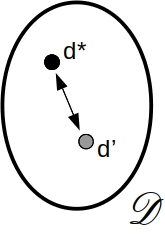
\includegraphics[scale=0.5]{surfeit}
\caption{\label{fig:intro-surfeit}Surfeit of a model.}
\end{figure}

Given an entity $e$, and one of its representations $r$, we define the \emph{surfeit}\index{Surfeit} of the description $d$ for the representation $r$, denoted by $\sigma(d, r)$, by:
\[
\sigma\left(d, r\right) = \frac{l \left(d\right) - K(r)}{l \left(d\right)}
\]

where $l \left(d\right)$ is the length (number of symbols) of the description $d$, and $K(r)$ is the length of the shortest possible description for $r$, that is, $d^\ast$. Since we are interested not only in measuring the surfeit of the description of individual representations, but also in comparing the surfeit of representations for multiple, potentially unrelated, entities, we have to divide the difference $l \left(d\right) - K(r)$ by the normalization factor $l \left(d\right)$. Unfortunately, in general, we do not know the shortest description of a representation, since our knowledge is incomplete, and so, surfeit is a quantity that has to be approximated in practice.

If we were able to come up with a perfect description for a representation, that string of symbols must be incompressible, otherwise it would contain superfluous elements that can be removed, and so, either it is not incompressible or it is not perfect. Given that an incompressible string is a random sequence of symbols (see Section \ref{sec:incompressibility_randomness}), an important consequence of our theory is that perfect knowledge implies randomness\index{Randomness}. The common understanding is that it is not possible to make sense from something that is random, since this is what randomness is all about. However, in the theory of nescience, by random description we mean a model that contains the maximum amount of information in the smallest space possible (it contains no redundant elements). Please mind that the converse does not hold; that is, a random description does not imply perfect knowledge. it might be possible we keep improving a theory until it becomes random, but later on we find a new and shorter theory (probably based on another encoding) that describes the same entity, and this new theory is not random yet.

Randomness effectively imposes a limit to how much we can know about a particular entity. Far from being a handicap, the proper understanding of this absolute epistemological limit is an opportunity to advance in our understanding of open problems. Moreover, since what is limited is the enhancement of our knowledge about already identified research entities, as opposed to the discovery of new ones (new entities are understood to be infinite), we can also apply our understanding of randomness to discover new research entities.

With our definition of surfeit, where longer explanations are worse, we are not suggesting that textbooks should always be as concise as possible. On the contrary, in some situations we expect textbooks to be highly redundant. A concise book is a text that contains a large amount of information in a very reduced space, and so, it is very difficult for humans to assimilate (understand) that information. However, a redundant textbook (like this one) contains the same amount of information but in a lager space, and so, it is easier to grasp it contents. Moreover, in some knowledge areas other than science, redundancy could be desirable. For example, in law, redundancy helps lawyers memorize legal texts, and in music, repetition could be a good thing for harmony, for example in a canon.

The concept of surfeit can be extended to research areas a well, in such a way that we can not only compute the surfeit of a given area as a whole, but also compare the surfeit of multiple, unrelated, areas.

\begin{example}
Based in the concept of "category" of Wikipedia, that it is quite similar to our concept of "research area", we could compute the surfeit of the major scientific areas (see Chapter \ref{chap:Redundancy} for more information about how to compute surfeit in practice). For example, as it is shown in Table \ref{tab:Redundancy_Areas}\footnote{Data from October 2014.}, in general our understanding of Mathematics is higher than our understanding of Computer Science, since the redundancy of Mathematics is 0.351 and the redundancy of Computer Science is 0.443. The concept of redundancy applied to areas largely matches our intuitive notion of which knowledge areas are better understood.
\end{example}

\begin{table*}
\begin{centering}
\begin{tabular}{|c|c|}
\hline 
Kowledge Area & Redundancy \tabularnewline
\hline 
\hline 
Mathematics & $0.351$ \tabularnewline
\hline 
Computer Science & $0.443$ \tabularnewline
\hline 
Chemistry & $0.466$ \tabularnewline
\hline 
Biology & $0.475$ \tabularnewline
\hline 
Psychology & $0.528$ \tabularnewline
\hline 
Epistemology & $0.530$ \tabularnewline
\hline 
Sociology & $0.543$ \tabularnewline
\hline 
\end{tabular}
\par\end{centering}
\caption{\label{tab:Redundancy_Areas}Redundancy of Scientific Areas}
\end{table*}

%
% Section: Nescience
%

\section{Nescience}
\label{sec:ch1_nescience}

Nescience is an old fashioned English word meaning “lack of knowledge or awareness”. In this sense, it seems to mean exactly the same as the word "ignorance", however there is a subtle difference: ignorance refers the lack of knowledge when knowledge is there (we do not know but we could learn, for example, by reading a book), and nescience refers to the lack of knowledge when knowledge is not there (we do not know, and it is not possible to know, since nobody knows). The theory of nescience has been developed with the aim of quantitatively measuring how much we do not know when knowledge is not there, that is, to quantify how much we, as humankind, do not know.

Intuitively, how much we do not know about an entity has to be computed based on the miscoding, inaccuracy and surfeit of a representation and a description, since those metrics summarize all possible types of mistakes we can make. Miscoding because it tell us how well the representation encodes the original entity under study; inaccuracy because it says how well the description models the representation; and surfeit because it tell us how good is the description itself. The best combinations of representations and descriptions are those who present a low miscoding, low inaccuracy and low surfeit. Unfortunately, those quantities are conflicting, in the sense that if we reduce one of them, the others may increase. For example, if we use a more complex description usually the inaccuracy will decrease but the surfeit will increase.

A pair $(d, r)$ composed by a description and a representation is Pareto optimal\index{Pareto optimality} if there does not exist another pair $(d', r')$ such that decreases at least one of the components of nescience, that is miscoding, inaccuracy and surfeit, without increasing another component. We are interested in a local version of the concept of Pareto optimality, since it might happen that the description $d'$ is so far from the description $d$ that it does not represent anymore the entity $e$ encoded by $r$ (given the insight of the oracle).

Pareto optimality allow us to find a family of candidate pairs $(d, r)$ that provide good explanation of an entity $e$. However, in science we prefer to select a single description as the model of a research entity. In order to select that description we have to provide a utility function\index{utility function} that allow us to classify and order the candidate descriptions. The form of this utility function is something that depends on the area in which the theory of nescience is being applied. For example, in case of entities encoded as datasets (machine learning) a good candidate utility function is the harmonic mean (see Chapter \ref{chap:Machine-Learning}). The \emph{harmonic nescience}\index{Nescience} of the representation $r$ given the description $d$ , denoted by $\nu_H\left(d, r\right)$, is defined as:
\[
\nu_H\left(d, r \right) = \frac{3}{ \mu(r)^{-1} + \iota(d, r)^{-1} + \sigma(d, r)^{-1}} 
\]
In the practice of science, we usually fix $r$ and talk about the nescience of the representation $r$ instead of the original entity $e$. If we have multiple candidate models $d_1, d_2, \ldots, d_n$ for the representation $r$, we say that our \emph{current best description}, denoted by $\hat{d}$, is the description that present the lowest nescience given a representation $r$.

\begin{example}
\label{cha1:ex:Boston}
{\color{red} TODO: Review this example.}
We are interested in understanding which are the factors that affect the price of houses. The encoding of that topic will be given by a dataset corresponding to 506 random samples taken from the suburbs of Boston\index{Boston dataset}. For each sample, 14 attributes have been measured, like for example the average number of rooms per dwelling, the per capita crime rate by town or the accessibility to radial highways. Our models will be based on a decision tree (a collection of nested if-else clauses), showing which are the most relevant factors that affect the price. The problem at hand is to identify the ideal depth of that tree, that is, how many if-else decision we should allow in the model that explain the behavior of prices. In order to do that, we compute the best trees from a depth level of 2 to a depth level of 8. In Table \ref{tab:Nescience_Models} left we have a plot of the mean squared error of the best model at each level, using different subsets for training and testing in order to avoid the overfitting of models. As we can see, the optimal level is 5, since increasing beyond this point means that there will be almost no further gain. In Table \ref{tab:Nescience_Models} right we can see the same study but applying our concept of nescience. In this latter case, we see that the optimal level is 3. That is, beyond that level it might be possible that our error decreases, but the model becomes so complex that it makes interpretation very difficult, and so, our understanding of the topic does not increase\footnote{Please mind that nescience and interpretability are not equivalent concepts, in the sense that we can find models with very low nescience that it are beyond the human capabilities of interpretation.}.
\end{example}

\begin{table*}
\begin{centering}
\begin{tabular}{c c}
\centering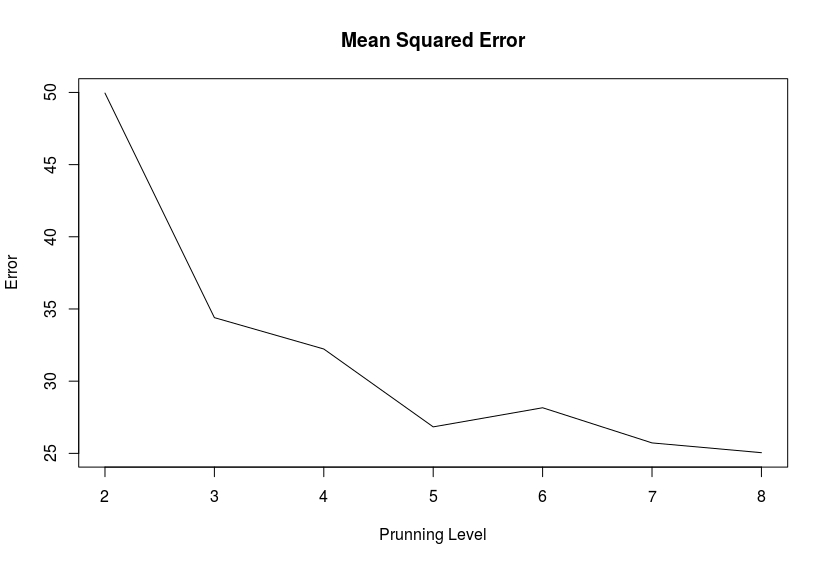
\includegraphics[scale=0.25]{Chapter1_MSE}
&
\centering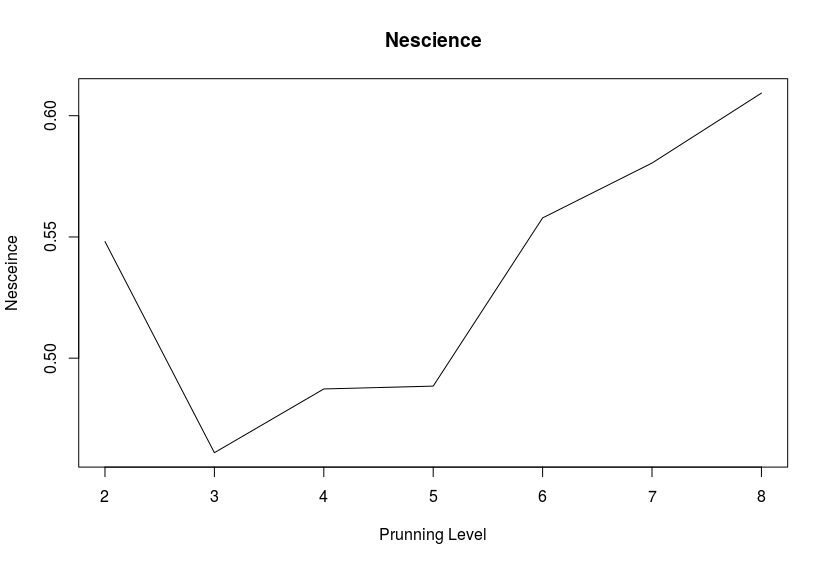
\includegraphics[scale=0.25]{Chapter1_Nescience}
\end{tabular}
\par\end{centering}
\caption{\label{tab:Nescience_Models}RMSE and Nescience of Models}
\end{table*}

We are interested in comparing the nescience, i.e. how much we do not know, of different research entities. For example, mathematicians claim that we do not know almost anything about differential equations, and sociologists claim that we do not know almost anything about the causes of armed conflicts. As it is shown in Example \ref{ex:diffeq_world}, this "we do not know almost anything" is much higher in case of armed conflicts than differential equations.

\begin{example}
\label{ex:diffeq_world}
We can compare how well we understand the "causes of the first world war" with how well we understand the "dynamics of populations", in this particular example, represented by the Lotka–Volterra differential equation\index{Lotka–Volterra differential equation}. In order to compare in practice these research topics we need a description, as complete and accurate as possible, of our current understanding about them. In case of abstract objects, we could use as descriptions the ones contained in reference works, since what we need is an encyclopedic coverage. For this example, we have used the descriptions found in the corresponding pages of the Wikipedia online encyclopedia\footnote{https://en.wikipedia.org/wiki/Causes\_of\_World\_War\_I (retrieved on August 2017)},\footnote{https://en.wikipedia.org/wiki/Lotk-Volterra\_equations (retrieved on August 2017)}. After a pre-processing of the original text, in which Wikimedia tags were removed, the files were compressed with the 7z compression utility (see Chapter \ref{chap:philosophy-science} for a detailed description of this process). Given this approach we have estimated that the redundancy of the causes of the first world war is 0.67, and the redundancy of the dynamics of population is 0.59. Those numbers suggest that we know better how the dynamics of populations work that the causes of this particular armed conflict. Unfortunately, not only is redundancy an approximation of surfeit, but also, in order to fully characterize our unknown we have to take into account the error of both descriptions. Moreover, it might happen that these pages at Wikipedia are not the best current descriptions available for those topics.
\end{example}

When the nescience of a representation $r$ is equal to zero ($\nu(d, r)=0$), we say that we have reached a \emph{perfect knowledge}\index{Perfect knowledge} about an entity. In practice it is not possible to know when we have reached the shortest possible description of the best possible valid representation, that is, when we have found the ultimate theory, since representations require to query the oracle, and descriptions are based on the uncomputable Kolmogorov complexity.

%
% Evolution of Nescience
%

\section{Evolution of Nescience}

In this book we assume that the final objective of science is to discover those descriptions and representations with the lowest possible nescience. The general approach is to produce a series of candidate descriptions and representations over time, each one with a lower nescience than the previous one, until perfect knowledge is reached. New descriptions could be based on novel theories that explain the entity, refinements over already existing ones, reducing the number of assumptions, etc. Nescience can also decrease by means of discovering better representations of the entities under study.

If performed properly, the nescience of an entity should be strictly decreasing as new descriptions and representations appear, since we should not accept a new description or representation as an improvement over the existing ones unless it reduces the nescience. It might happen that a new description presents a higher surfeit, or a higher inaccuracy, but never both things at the same time, since that would imply a higher nescience. Of course, in practice things are not that easy, since our current values of miscoding, inaccuracy and surfeit as just estimations of the real values, and they could be wrong estimations. For a practical point of view, we only require that nescience decrease over time on average.

\begin{example}
The concept of nescience can be applied to measure how well we understand current computer software, like for example operating systems, databases, or productivity applications. The surfeit of the software could be based on the compressibility of the source code, and the inaccuracy on the number of bugs found. In Figure \ref{fig:Chapter1_SQLite} we can see the evolution of the nescience in the latest published versions of the open source database SQLite\footnote{www.sqlite.org}. As we can observe (given the regression line) the nescience of SQLite decreases with time, and so, we can conclude that as new versions appear this application better solves the problem at hand. In Chapter \ref{chap:Software-Engineering} we will see that this is not the case for most of the existing software platforms and applications.
\end{example}

\begin{figure}[h]
\centering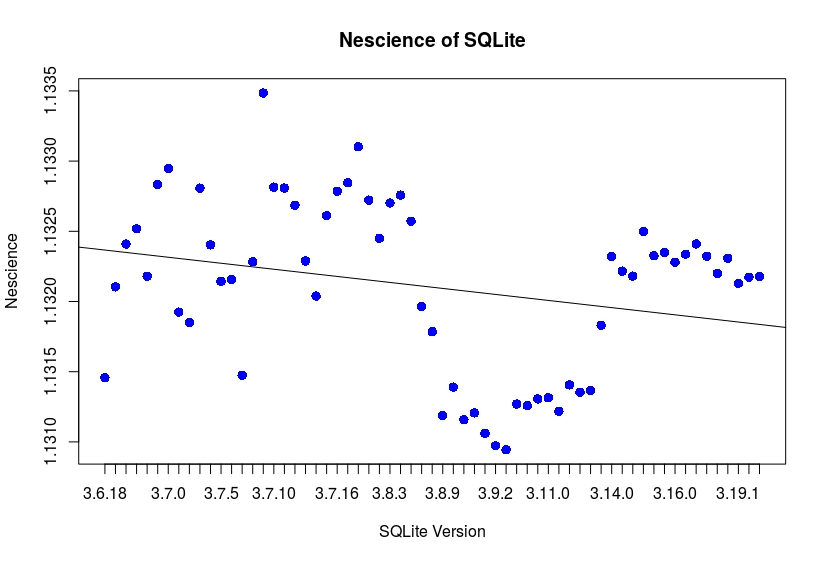
\includegraphics[scale=0.35]{Chapter1_SQLite}
\caption{\label{fig:Chapter1_SQLite}Evolution of Nescience}
\end{figure}

We can use this property of reduction of nescience as a characterization of what constitutes a valid scientific discipline and what is not (what it is called the demarcation problem in philosophy of science). In case of non-scientific theories (pseudosciences and others) nescience does not decrease, on average, when new representations or new descriptions are available. That is, in pseudosciences we do not learn anything new when we do further research.

\begin{example}
A trading robot is a computer program that gets as input real time quotes from the stock markets, or foreign currency exchanges, and based on an algorithm decides how to invest money, in general by means of opening very short-time positions (what it is called intra-day trading). Many of these robots are based on technical indicators, that is, metrics that are derived from current and past prices (like moving averages, or resistance levels) to forecast future prices. It is an open question if it is possible to make any money using those robots, that is, if they have a positive mathematical expectancy sufficiently high to cover brokers commissions. We can study this problem with the aid of the theory of nescience. In order to do that, we have randomly selected 40 trading robots developed over a period of 6 years, and we have tested them (see Section \ref{sec:trading} for more information). In Figure \ref{fig:Chapter1_EA} we can see the evolution of the nescience of these robots along time. As we can observe, nescience does not decrease, in fact it increases.
\end{example}

\begin{figure}[h]
\centering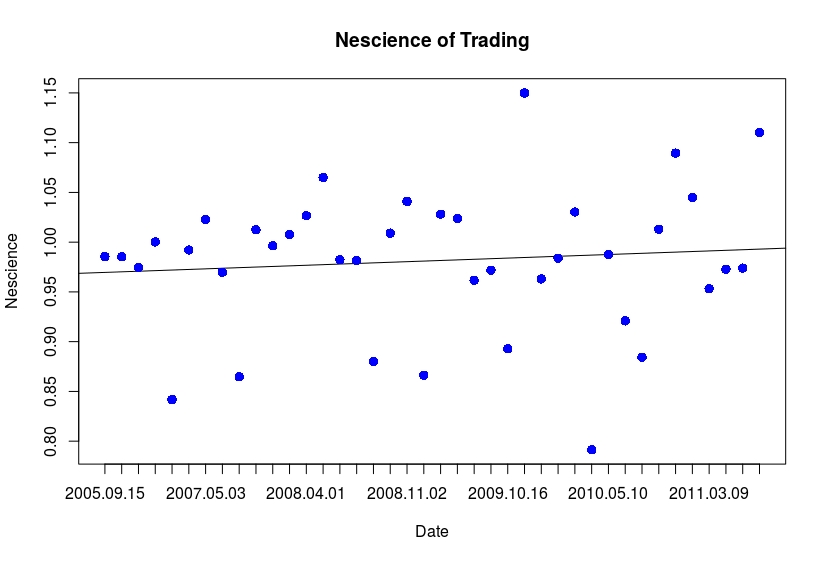
\includegraphics[scale=0.35]{Chapter1_EA}
\caption{\label{fig:Chapter1_EA}Nescience of Forex Trading Robots}
\end{figure}

%
% Section: Other Metrics
%

\section{Other Metrics}

Nescience is a metric that can be used to identify the most interesting topics from the point of view of research. Since nescience is a measure of our ignorance about a topic, the higher the nescience the more opportunities for research. In this section we are going to propose other metrics that can complement nescience in the task of measuring the interest of research topics. These metrics will be helpful, not only for the classification of individual research topics, but also for the development of a methodology for the discovery of potential solutions to open problems (Section \ref{sec:intro_interesting_questions}), and the discovery of new research topics (Section \ref{sec:intro_research_topics}).

One of these new metrics for the classification of research topics is \emph{relevance}. Relevance is a measure of the impact that a topic has on people's life. Intuitively, the higher the relevance of a topic, the higher its potential as a source of interesting problems, since we will be working on problems that affect many people directly. In order to measure the impact of a research topic we have to construct what we call the relevance graph, a figure that describes how people are affected by research topics (see Figure \ref{fig:Relevance-Graph_Intro}).

\begin{figure}[h]
\centering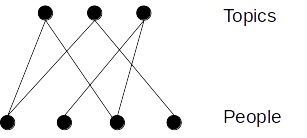
\includegraphics[scale=0.7]{bipartite_graph}
\caption{\label{fig:Relevance-Graph_Intro}Relevance Graph}
\end{figure}

The relevance graph connects all known topics and all possible human beings. A link between a topic and a person means that this person is affected by the topic, not that he is interested in this particular topic. For example, somebody that is trying to find a cure to diabetes will not be connected to the research topic diabetes, however, somebody that actually suffer from diabetes will be. The higher the relevance of a topic, the higher its potential as a source of interesting problems to solve. In this sense, the research topic "how to cure diabetes" is more relevant that the research topic "how far dog fleas can jump", since more people are affected by the former than by the latter. The exact meaning of "\emph{being affected by}" is an abstract concept that has to be approximated in practice. For example, we could claim that the wife of a man that has diabetes is somehow affected by the disease as well. In Part \ref{part:Applications} of this book we will see some examples of how to approximate this abstract quantity.

Given these two metrics, nescience and relevance, we can provide a quantitative measure of the interestingness of a topic as a source of interesting problems, that is, how likely is that the topic can be used as part of a new interesting research project. We define this quantity as a function of the relevance and nescience of the topic (for example, the normalized product of both quantities). Intuitively, a topic is interesting as a source of new problems if it has a large relevance (it has high impact in people's life) and a large nescience (it is not very well understood). In Figure \ref{fig:Interestingness-Questions} is graphically depicted the idea. For example, the Pythagoras' theorem has some relevance, since people life's can be indirectly affected by its implications, but since it is a very well understood theorem (our nescience is very low), it is not a very interesting research topic by itself. The World War I is very relevant, because it had a huge impact on many people's life, and also it is not very well understood topic as we have seen in Example \ref{ex:diffeq_world}. So, according to our definition, it has a huge potential as a source of new interesting research problems.

\begin{figure}[h]
\centering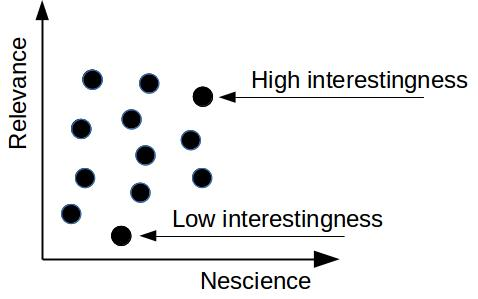
\includegraphics[scale=0.5]{InterestQuestions}
\caption{\label{fig:Interestingness-Questions}Interestingness of Topics}
\end{figure}

\begin{example}
\label{ex:wikipedia-problems}
We can use the collection of Wikipedia articles to identify topics that are interesting as a source of new problems. The starting point of our analysis is the classification contained in the scientific disciplines category of Wikipedia. This category is organized\footnote{Data from November 2014.} into the following main areas: "applied sciences", "behavioral sciences", "cognitive sciences", "formal sciences", "natural sciences", "physical sciences", and "social sciences". In order to evaluate the classification metrics proposed we have used the set of topics corresponding to all pages under any of the subcategories contained in the category "theory of computation" (a subcategory of the category "theoretical computer science", that belongs to the area "formal sciences"). Pages were cleaned up using the same procedure described in Example \ref{ex:diffeq_world}, and the relevance was estimated based on the number of unique visits to each page (please, refer to Chapter \ref{chap:philosophy-science} for more information about this process). Topics that fit our intuitive idea of problem, that is, not very well understood concepts with a high relevance, could include "arithmetical hierarchy" (0.72), "halting problem" (0.65), "floating point" (0.61), "quantum computer" (0.57), and "computable function" (0.55).
\end{example}

The Pythagoras' theorem is not a very interesting research topic by itself, however, it is a very important theorem, since it can be applied to solve many practical problems. A new metric is required to capture this concept of topic that is important because it can be used as a tool to solve other problems. We define the \emph{maturity} of a topic as the inverse of nescience. Intuitively, the more mature a topic is the higher its potential applicability as a tool to solve other open problems, since we know very well how the topic works and how it can be successfully applied. In general, highly immature topics should not be applied to solve open problems, since they could provide wrong answers.

Besides maturity, we also introduce the metric of \emph{applicability} of a topic. Applicability is based on the concept of \emph{applicability graph}. An applicability graph is a directed graph between the research topics (see Figure \ref{fig:ApplicabilityGraph}). An arrow between two topics means that the first topic been successfully applied to explain or solve the second topic. For example, the topic “graph theory” has been applied to the topic “recommendation engines”, since graph theory has been used to solve the problem of which products we should advertise to potential customers on Internet. Given this graph, we define the applicability of a topic as the number of problems to which the topic has been successfully applied. The higher the applicability of a topic, the higher its potential as a tool that can be applied to solve new problems.

\begin{figure}[h]
\centering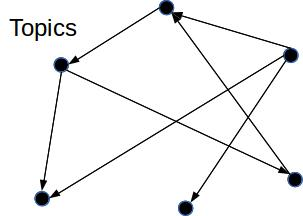
\includegraphics[scale=0.5]{ApplicabilityGraph}
\caption{\label{fig:ApplicabilityGraph}Applicability Graph}
\end{figure}

Finally, we define the concept of interestingness of a topic as a source of interesting tools, that is, how likely is that the topic can be used to solve a new problem, as a function of its maturity and applicability. Intuitively, a topic is interesting as a tool if it has been already applied to many other problems, and it is very well understood topic. For example, the Pythagoras' theorem, although not very relevant as a source of interesting problems, it is very relevant as a source of new applications to other open problems.

\begin{example}
We can use the collection of Wikipedia scientific articles to identify topics with high potential as tools. The procedure used in this example is similar to the one described in Example \ref{ex:wikipedia-problems}, except that the metric applicability has been estimated based in the collection of internal links within Wikipedia itself. The rationale is that if a page is referenced many times by other Wikipedia pages, it is highly likely that it contains useful information. Using this procedure, some examples of topics with high interest as tools in the area of theoretical computer science include "recursion" (0.42), "state space" (0.42), "abstract machine" (0.41), or "ternary numeral system" (0.48).
\end{example}

%
% Section: Interesting questions
%

\section{Interesting Research Questions}
\label{sec:intro_interesting_questions}

In the theory of nescience we distinguish two kinds of unknowns, the \emph{known unknown} and the \emph{unknown unknown}. By known unknown we mean all those already known problems for which we do not know their solutions, for example, nobody knows how to cure diabetes, but we know what diabetes is and we are aware that nobody knows how to cure it. By unknown unknown we mean the collection of unknown problems, that is, all those problems that have not been found yet, like for example the Eldermeyer's disease\footnote{We cannot say anything more about the Eldermeyer's disease, since Dra. Eldermeyer will born next year, and it will take her 34 years more to discover the disease named after her.}. The area composed by the unknown unknown problems is a highly interesting one, since it contains those research topics that will be addressed in the future. One of the main goals of this book is to help scientists discover the topics that lay in this unknown unknown area, since that would bring to the present the research problems of the future (see Section \ref{sec:intro_research_topics}). In this section we focus on how to solve the problems of the known unknown area.

An \emph{interesting question} is a ordered pair of topics $t$ and $p$, where $t$ has a high interestingness as tool, and $p$ has high interestingness as problem. Intuitively, the questions would be something like “can we apply the tool described by topic $t$ to solve the problem described by topic $p$?”. The interestingness of the new questions will be measured by means of a function of the interestingness of $t$ and $p$ themselves. In practice what we have to do is to compute all the possible combinations of tools and questions and select those with higher combined interestingness (see Figure \ref{fig:InterestingQuestions}).

\begin{figure}[h]
\centering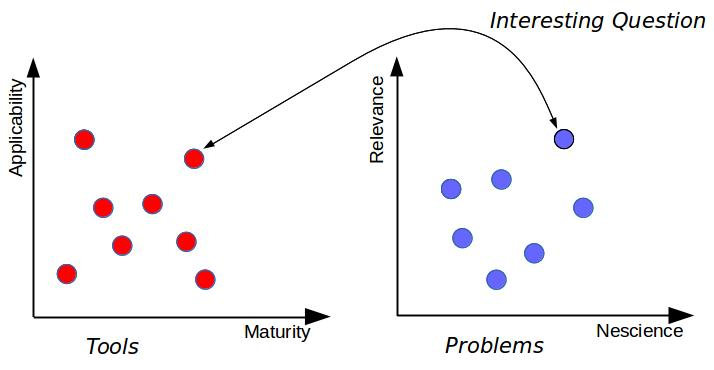
\includegraphics[scale=0.5]{InterestingQuestions}
\caption{\label{fig:InterestingQuestions}Interesting Questions}
\end{figure}

An interesting question is \emph{intradisciplinary} if it combines two topics that are studied in the framework of the same research area (e.g., computer science). An interesting question is \emph{interdisciplinary} if it combines two topics of different research areas (e.g., computer science and philosophy). In principle, the most innovative questions would be interdisciplinary questions, because the probability that somebody has thought about them is lower, since it requires specialists in both research areas working together to come up with that particular question.

\begin{example}
We could combine the topics with high interestingness as tools found in the area of "computer science" with those topics with high interestingness as problems found in the area of "biochemistry" in order to find new interesting interdisciplinary questions. Some examples of the kind of questions we can find with this approach include: “can we use regular expressions to identify DNA genes?” or “can we use a recursive algorithm to characterize proteins tertiary structure?”
\end{example}

Once we have identified an interesting research question, we could use the concept of \emph{conditional model} to see if the tool can help us to understand, or solve, the open problem. A conditional model of a topic $t$ given a perfect model of a second topic $s$ is also a string in the form $\langle TM,a \rangle$, but in this case we require that $TM \left(\langle m_s^\star, a \rangle \right) = t$. That is, the Turin machine $TM$ is able to print $t$ when it has as input both, the incompressible part $a$, and a perfect model $m_s^\star$ for the topic $s$. If the conditional complexity of the open problem given the tool is smaller than its original complexity, then the tool is helpful to solve the problem. The more the tool reduce the length of the conditional model with respect to the original model, the better.

Please note that the methodology presented here is a generic one, in the sense that it can be applied to multiple domains, not only to the discovery of new interesting research questions. The metrics and methods described can be applied to any area where there is a large collection of interrelated describable objects and we are interested in discovering new, previously unconsidered, objects. The exact definition of concepts like relevance graph, applicability graph or maturity will depend on the area in which the methodology is being applied. In Part \ref{part:Applications} of this book, we will describe some examples of other applications, for example, to the identification of new software quality tests.

%
% Section: New Research Entities
%

\section{New Research Entities}
\label{sec:intro_research_topics}

We have mentioned in the previous section the existence of an \emph{unknown unknown} area composed by those problems that not only we do not know how to solve them, but also we are not even aware they exist. We are interested in providing a procedure to discover new research entities located in this important area. A possible approach could be by randomly selecting a binary string and asking to the oracle if that string is close to the representation of a (hopefully unknown) entity. However, given the huge amount of candidate strings, that procedure is not feasible in practice.

In this book we will investigate an alternative approach, based on the combination of already known topics (see Chapter \ref{chap:Interesting-Research-Questions}), what we call \emph{joint topics}. If $r_1, r_2 \in \mathcal{R}$ are two different representations of two different entities, the joint topic of $r_1$ and $r_2$ is the concatenated string $r_1 r_2$ (see Figure \ref{fig:intro_new_topics})\footnote{As we will see in Chapter \ref{cha:Topics-and-Descriptions}, we require $\mathcal{R}$ to be closed under the operation of concatenation of representations, that is, for any two representations $r, s \in \mathcal{R}$ we have that $rs \in \mathcal{R}$.}. For example, if $r_1 \in \mathcal{R}$ is a representation of the entity "maximum entropy", and $r_2 \in \mathcal{R}$ a representation of the entity "probability distribution", the entity represented by the joint topic $r_1 r_2$ would be "maximum entropy probability distribution".

\begin{figure}[h]
\centering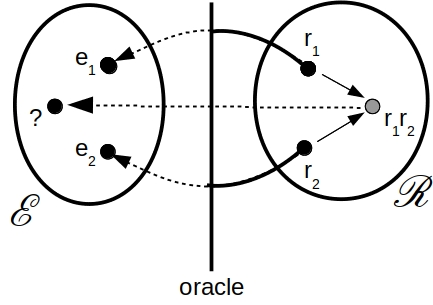
\includegraphics[scale=0.5]{new_topics}
\caption{\label{fig:intro_new_topics}Discovering new research entities.}
\end{figure}

A \emph{new research topic} is a topic that lies in the unknown unknown area. Since the surfeit (resp. inaccuracy) of joining two topics is higher than the superfeit (resp. inaccuracy) of any of them isolated, we can identify new interesting research topics by combining already existing interesting problems (see Figure \ref{fig:NewTopics}). Formally, a new research topic is unordered pair of topics $r_1$ and $r_2$, where both $r_1$ and $r_2$ have a high interestingness as problems. In practice, we have to compute all the possible combinations of those problems with very large interestingness with themselves, and select the ones with the higher potential. The exact meaning of the new topic that results by merging existing problems is something that has to be discovered with further research.

\begin{figure}[h]
\centering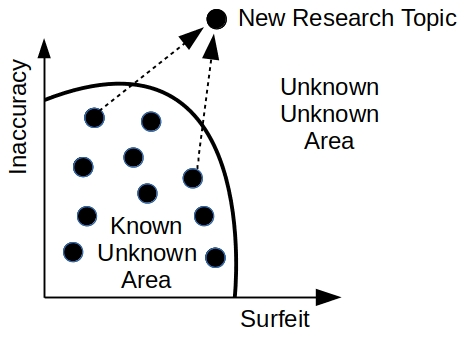
\includegraphics[scale=0.5]{NewTopics}
\caption{\label{fig:NewTopics}New Research Topics}
\end{figure}

\begin{example}
We could combine the most interesting topics of the area of "theoretical computer science" with the most interesting topics of the area "phenomenology" in order to identify the most promising combinations. Fore example, by combining "minimum complexity computer programs" and "self awareness" we obtain that a potential new research topic could be “minimum complexity self-aware computers”; that is, investigating the minimum complexity required for a computer program to have the capacity of being self-aware.
\end{example}

We can extend our method to find new research topics with additional metrics. For example, by means of adding the relevance of topics, we could discover new interesting research topics that are also relevant.

%
% Section: References
%

\section{References and Further Reading}

The idea that perfect descriptions must be random has been already mentioned by other authors (see for example \cite{mosterin2016conceptos}). The gravity dataset used in Example \ref{ex:introduction:inaccuracy:newton} comes from \cite{cressie1982playing}, and a more detailed analysis can be found at \cite{davison1997bootstrap}. The Boston housing dataset referred in Example \ref{cha1:ex:Boston} was published in \cite{harrison1978hedonic} and further discussed in \cite{belsley2005regression}; for more information about decision trees see for example \cite{james2013introduction}. For more information about trading systems and technical indicators see for example \cite{kaufman2013trading}, and how to quantitatively test if a system is profitable to \cite{pardo1992design}. The Locka-Voterra model for population dynamics was originally described in \cite{lotka1920analytical}. How to apply graph analysis to recommendation engines is covered in \cite{cordobes2015empirical}. And finally, if the reader is interested in knowing how far a dog flea can jump, please refer to \cite{cadiergues2000comparison}.

The discipline of epistemology is more oriented to understand what we do know as individuals, meanwhile in this book we are interested in what we know as humankind; moreover, the kind of knowledge addressed by epistemology is not necessarily the scientific knowledge subject of the theory of nescience. Perhaps, the area of epistemology more interesting for our purposes is what the epistemologists call knowing by testimony. A good, and easy to read, introduction to the discipline of epistemology is \cite{nagel2014knowledge}.






%
%
% PART 1.- BACKGROUND
%
%

\part{\label{part:Background}Part 1: Background}


%
% CHAPTER: Preliminaries
%

%
% CHAPTER: Preliminaries
%

\chapterimage{Koenigsberg_Map_by_Bering_1613.pdf} % Chapter heading image

\chapter{Discrete Mathematics}
\label{chap:Discrete_Mathematics}

\begin{quote}
\begin{flushright}
\emph{Mathematics may be defined as the subject in which\\
we never know what we are talking about,\\
nor whether what we are saying is true.}\\
Bertrand Russell
\end{flushright}
\end{quote}
\bigskip

Most of the mathematics used throughout this book belong to the area of \emph{discrete mathematics}. Discrete mathematics is characterized because it studies mathematical objects that have distinct or separated values, rather than continuous. Examples of discrete objects used in this book are integers, strings, graphs and computer programs. A key distinctive element of discrete sets is that they can be enumerated with natural numbers, that is, they are countable. We will barely use continuous mathematics, for example calculus, in the theoretical developments of the theory of nescience.

Our main interest in discrete mathematics is because computers. The theory of nescience borrows concepts and ideas from multiple areas of computer science: algorithms, coding, string complexity and others. Computers operate in discrete steps and the data processed is stored in discrete units of memory. We are interested in computers because we want to apply our theoretical developments to as many real objects as possible, and we think that the right way to model our world is by means of using computers. In pure mathematics it is customary to discuss abstract objects without worrying about what they represent. In the theory of nescience, on the contrary, the representation (encoding) of objects plays a crucial role.

This chapter is intended as a quick review of the basic concepts of discrete mathematics; no formal definitions are provided and theorems are not proved. Discrete mathematics is an extremely diverse and large area of study. We will review only those elements that are required to understand the theory of nescience. Some of the theories involved (computability, information, complexity, ...) require a deeper coverage, and so, they are studied in separate chapters. In the References section there is a list of suggested books that explain in detail the topics covered in this chapter.

%
% Section: Sets
%

\section{Sets, Relations and Functions}
\label{sec:sets}

The sets of \emph{natural}\index{Set of natural numbers}, \emph{integers}\index{Set of integers}, \emph{rational}\index{Set of rationals}, and \emph{real}\index{Set of real numbers} numbers are represented by $\mathbb{N}$, $\mathbb{Z}$, $\mathbb{Q}$, and $\mathbb{R}$ respectively, which includes the number $0$. The \emph{positive integers}\index{Set of positive integers} are denoted by $\mathbb{Z}^+$, and the \emph{positive reals}\index{Set of positive reals} by $\mathbb{R}^+$, where both of these sets incorporate the number $0$. Let $A$ be a \emph{set}\index{Set}. We signify that $x$ is an \emph{element}\index{Element of a set} of $A$ by the notation $x\in A$, and that $x$ is not an element of $A$ by $x \notin A$. Elements of a set can be enumerated using braces, such as $A = \{0, 1, 2, 3\}$, or they can be defined by conditions via the \emph{set-builder}\index{Set formation notation} notation, for instance $A = \{x \in \mathbb{N} : x < 4\}$, with the stipulation that the \emph{universe}\index{Universe of a set} of the set be clearly established.

Suppose $A$ and $B$ are two sets. We use the notation $A = B$ to denote that the sets are \emph{equal}\index{Equal sets}. The expression $A \subseteq B$ signifies that $A$ is a \emph{subset or equal}\index{Subset} to $B$, and $A \subset B$ is used to indicate that $A$ is a \emph{proper subset}\index{Proper subset} of $B$ (implying $A$ is not equivalent to $B$). The condition $A = B$ holds true if, and only if, both $A \subseteq B$ and $B \subseteq A$ are satisfied concurrently. The symbol $\varnothing$ represents the \emph{empty set}\index{Empty set}, a set that contains no elements.

\begin{example}
For every set $A$ we have that $\varnothing \subseteq A$ and $ A \subseteq A$.
\end{example}

The term \emph{cardinality}\index{Cardinality of a set} refers to the number of elements within a finite set $A$, denoted as $d(A)$. Accordingly, the cardinality of the empty set $\varnothing$ is 0, as it contains no elements. For any two sets $A$ and $B$, the notation $A \cup B$ signifies the \emph{union}\index{Union of sets} of $A$ and $B$, whereas $A \cap B$ designates the \emph{intersection}\index{Intersection of sets} of $A$ and $B$. When dealing with $n$ sets, say $A_1, A_2, \ldots, A_n$, their union and intersection are denoted as $\cup_{i=1}^n A_i$ and $\cap_{i=1}^n A_i$ respectively. For an arbitrary collection of sets indexed by $I$, we employ $\cup_{i \in I} A_i$ and $\cap_{i \in I} A_i$. In the context of an infinite collection of sets, the notations $\cup_{i}^{\infty} A_i$ and $\cap_{i}^{\infty} A_i$ are adopted.

On occasion, we will resort to the use of \emph{Venn diagrams}\index{Venn diagram} as a visual means to represent sets, as exemplified in Figure \ref{fig:Venn-diagram}.

\begin{figure}[t]
\centering
\begin{tikzpicture}

    % Rectangle with label
    \draw (0,0) rectangle (5,3.5) node[below left] {$\mathbb{N}$};
    
    \fill[gray!30] (1.75,1.75) circle (1);
    \fill[gray!30] (3.25,1.75) circle (1);

    \node[draw, circle, minimum width=2cm, label=center:{$A$}] at (1.75, 1.75) {};
    \node[draw, circle, minimum width=2cm, label=center:{$B$}] at (3.25, 1.75) {};

\end{tikzpicture}
\caption{\label{fig:Venn-diagram}Representation of $A \cup B$ as a Venn Diagram}
\end{figure}


Given the sets $A$ and $B$, $A \backslash B$ is the \emph{set difference}\index{Set difference}, and ${A}^c$ is the \emph{complement}\index{Complement of a set} set of $A$. The \emph{De Morgan's laws}\index{De Morgan's laws} state that for every two sets $A$ and $B$ we have that $\left( A \cup B \right)^c = A^c \cap B^c$ and $\left( A \cap B \right)^c = A^c \cup B^c$.

Two sets $A$ and $B$ are \emph{disjoint}\index{Disjoint sets} if $A \cap B = \varnothing$. The sets $A_1, A_2, \ldots, A_n$ are disjoint if for every $i$ and $j$ such that $i \neq j$ we have that $A_i \cap A_j = \varnothing$. A \emph{partition}\index{Partition of a set} of a set $A$ is a collection of nonempty disjoint subsets of $A_1, A_2, \dots, A_n$ of $A$ such that  $A = \cup_{i=1}^n A_i$. The \emph{power set}\index{Power set} $\mathcal{P}(A)$ is the set whose members are all possible subsets of A. If $d(A)=n$ then $d\left( \mathcal{P}(A) \right) = 2^n$.

Given any two sets $A$ and $B$, we denote the \emph{set difference}\index{Set difference} as $A \backslash B$, and the \emph{complement}\index{Complement of a set} of the set $A$ as ${A}^c$. \emph{De Morgan's laws}\index{De Morgan's laws} articulate that for any pair of sets $A$ and $B$, we have $\left( A \cup B \right)^c = A^c \cap B^c$ and $\left( A \cap B \right)^c = A^c \cup B^c$.

The term \emph{disjoint}\index{Disjoint sets} is applied to two sets $A$ and $B$ when their intersection $A \cap B = \varnothing$. We say that the sets $A_1, A_2, \ldots, A_n$ are disjoint if for every distinct pair $i$ and $j$ ($i \neq j$), we find $A_i \cap A_j = \varnothing$. A \emph{partition}\index{Partition of a set} of a set $A$ is an assembly of nonempty disjoint subsets $A_1, A_2, \dots, A_n$ of $A$ satisfying  $A = \cup_{i=1}^n A_i$. The \emph{power set}\index{Power set} of $A$, denoted as $\mathcal{P}(A)$, is the collection of all conceivable subsets of $A$. If the cardinality of $A$ is $n$, i.e., $d(A)=n$, then the cardinality of the power set of $A$ is $2^n$, thus expressed as $d\left( \mathcal{P}(A) \right) = 2^n$.

\begin{example}
Given the set $A = \{1, 2, 3\}$, its power set is:
\[
\mathcal{P}(A) = \{\varnothing, \{1\}, \{2\}, \{3\}, \{1,2\}, \{1,3\}, \{2,3\}, A\}
\]
\end{example}

Consider a non-empty set $A$ and a collection $\mathcal{F}$ of subsets of $A$. The pair $\left( A, \mathcal{F} \right)$ is designated as an \emph{field}\index{Field of sets} over $A$ if it fulfills the following conditions: it includes the empty set, denoted as $\varnothing \in \mathcal{F}$, it is closed under the operation of complementation, meaning for each $F \in \mathcal{F}$, the complement $F^c  \in \mathcal{F}$, and it is closed under finite unions, which indicates $F_1 \cup \ldots \cup F_n  \in \mathcal{F}$ for all subsets $F_1, \ldots, F_n \in \mathcal{F}$. Additionally, it can be demonstrated that a field also fulfills two further criteria: $A \in \mathcal{F}$, and it is closed under finite intersections, expressed as $F_1 \cap \ldots \cap F_n  \in \mathcal{F}$ for all subsets $F_1, \ldots, F_n \in \mathcal{F}$.

% Relations

Consider two elements, $x$ and $y$. An \emph{ordered pair}\index{Ordered pair}, symbolized as $(x, y)$, is a pairing of $x$ and $y$ in that order. By expanding this concept, an \emph{n-tuple}\index{n-tuple} — which can be visualized as an $n$-element ordered pair — is written as $(x_1, \ldots, x_n)$. We define the \emph{Cartesian product}\index{Cartesian product} of two sets $A$ and $B$, which is symbolized as $A \times B$. This product is a set consisting of all possible ordered pairs $(x, y)$, where $x$ belongs to set $A$ and $y$ belongs to set $B$. The Cartesian product can be extended to $n$ sets, $A_1, A_2, \dots, A_n$, and is expressed as $A_1 \times A_2 \times \dots \times A_n$. Moreover, the \emph{n-fold Cartesian product} of a set $A$ with itself is represented as $A^n$.

Let $R$ be a subset of the Cartesian product of set $A$ with itself, i.e., $R \subseteq A \times A$. Such a subset is referred to as a \emph{binary relation}\index{Binary relation}, which can be represented as $aRb$, meaning that the ordered pair $(a, b)$ is a member of $R$. A binary relation is deemed \emph{reflexive}\index{Reflexive relation} if for any element $a$ in $A$, it holds that $aRa$. It is termed \emph{symmetric}\index{Symmetric relation} if for all $a, b$ in $A$, the presence of $aRb$ automatically implies $bRa$. The property of \emph{antisymmetric}\index{Antisymmetric relation} is attributed to a binary relation when the coexistence of $aRb$ and $bRa$ leads to the conclusion that $a = b$. It is considered \emph{transitive}\index{Transitive relation} if for any $a, b, c$ in $A$, the occurrence of $aRb$ and $bRc$ infers $aRc$. A binary relation is identified as \emph{total}\index{Total relation} if for all $a, b$ in $A$, either $aRb$ or $bRa$ holds. Binary relations can be extended to include two different sets $A$ and $B$ as a subset $R \subseteq A \times B$, and can also be adapted to \emph{n-ary} relations represented as $R \subseteq A_1 \times A_2 \times \dots \times A_n$.

Let $R$ be a binary relation that is a subset of the Cartesian product $A \times A$, i.e., $R \subseteq A \times A$. If this relation is reflexive, symmetric, and transitive, it is designated as an \emph{equivalence relation}\index{Equivalence relation}, typically symbolized by $\sim$. Within the context of an equivalence relation, two elements $a, b$ from set $A$ are deemed \emph{equivalent}\index{Equivalent elements} if the relation $a \sim b$ holds. The notion of an \emph{equivalence class}\index{Equivalence class}, denoted as $[a]$, refers to the set of all elements in $A$ that are equivalent to a particular element $a$. In other words, the equivalence class of $a$ is defined as $[a] := \{ b \in A : a \sim b\}$. An equivalence relation serves to partition the base set into what is known as the \emph{quotient set}\index{Quotient set}. Represented as $A / {\mathord {\sim }}$, the quotient set consists of all equivalence classes stemming from elements of $A$, that is, $A / {\mathord {\sim }} := \{ [a] : a \in A \}$.

A binary relation that is reflexive, transitive, and antisymmetric is known as a \emph{partial order}\index{Partial order}, often represented by the symbol $\preceq$. A set equipped with a partial order is referred to as a \emph{partially ordered set}\index{Partially ordered set}, also abbreviated as \emph{poset}\index{poset}. In the context of a poset, an element $a$ from set $A$ is considered \emph{minimal}\index{Minimal element} if there is no other element $b$ in $A$ for which $b \preceq a$. Similarly, an element $a$ is labeled as \emph{maximal}\index{Maximal element} if no other element $b$ in $A$ exists such that $a \preceq b$. A relation that embodies reflexivity, transitivity, antisymmetry, and totality is designated as a \emph{total order}\index{Total order}, typically symbolized by $\leq$. A set that is coupled with a total order is identified as a \emph{totally ordered set}\index{Totally ordered set}. For any totally ordered set $A$, the \emph{maximum}\index{Maximum element} element is represented by $\max(A)$, meaning that $\max(A) \geq x$ holds for all $x$ in $A$. Similarly, the \emph{minimum}\index{Minimum element}, represented by $\min(A)$, is defined as an element such that $\min(A) \leq x$ for all $x$ in $A$.

\begin{example}
Let $R$ be a relation that is a subset of the Cartesian product of the set of natural numbers $\mathbb{N}$ with itself, i.e., $R \subset \mathbb{N} \times \mathbb{N}$. In this relation, an ordered pair $(a, b)$ belongs to $R$ if $a$ is a divisor of $b$. The set $\mathbb{N}$, when paired with relation $R$, forms a partially ordered set. In this context, the number $11$ serves as a minimal element of $R$. This is because $11$ is a prime number, which, by definition, can only be divided evenly by 1 and itself.
\end{example}

% Functions

A \emph{function}\index{Function} is defined as a binary relation $f \subseteq A \times B$, where for each element $x \in A$, there exists at most one $y \in B$ satisfying the condition $\left(x, y\right) \in f$. In this context, elements $\left(x, y\right) \in f$ are denoted by $f(x)=y$, with the function represented by $f : A \rightarrow B$. The set $A$ is referred to as the \emph{domain}\index{Domain} of $f$, and $B$ is the \emph{codomain}\index{Codomain}. The set $\{ y \in B : \exists x \in A , f(x) = y\}$ constitutes the \emph{range}\index{Range} of $f$. If the relation is not defined for all $x \in A$, the function is termed \emph{partial}\index{Partial function}, denoted by $f(x) \uparrow$ for undefined $x$ in the function $f$. 

\begin{example}
In Section \ref{sec:computable_functions}, we will discuss an alternate interpretation of a function as a procedure, or a series of steps, that assigns an element of $B$ to each element of $A$. For instance, the subsequent C code delineates a partial function from $\mathbb{R}$ to $\mathbb{R}$, characterized as partial due to $inv(0)\uparrow$:
\begin{verbatim}
    double inv(double x) {
        return 1 / x;
    }
\end{verbatim}
\end{example}

A function is said to be \emph{injective}\index{Injective function} if, for all elements $x$ and $y$, $f(x) = f(y)$ implies $x=y$. A function is \emph{surjective}\index{Surjective function} when for every $y$, there exists at least one $x$ such that $f(x) = y$. A function is described as \emph{bijective}\index{Bijective function} if it exhibits both injective and surjective properties. The \emph{identity}\index{Identity function} function $I_A : A \rightarrow A$, determined by $f(a) = a$ for all $a \in A$, is bijective. These concepts of function, partial function, injective, surjective, and bijective can be extended to $n$-ary functions, represented as $f: A_1 \times A_2 \times \dots A_n \rightarrow B$.

The \emph{inverse}\index{Inverse function} function of a function $f$, represented by $f^{-1}$, is identified by $f(f^{-1}(x)) = f^{-1}(f(x)) = x$. Given two functions $f$ and $g$, where the domain of $f$ coincides with the range of $g$, we define the \emph{composition}\index{Composition} of $f$ with $g$, represented by $f \circ g$, as $f \circ g = f(g(x))$.

An infinite set $A$ is designated as \emph{countable}\index{Countable set} if there is a bijective function that maps the elements of $A$ onto the set of natural numbers $\mathbb{N}$. In contrast, a set is deemed \emph{uncountable}\index{Uncountable set} if it is not finite and also not countable. We refer to a set as having \emph{countably many}\index{Countably many set} elements if it is either finite or countable.

\begin{example}
Sets like $\mathbb{N}$, $\mathbb{Z}$ and $\mathbb{Q}$ are countable, while $\mathbb{R}$ is not.
\end{example}

The \emph{characteristic function}\index{Characteristic function} of a set $A$ is denoted as $1_A : A \rightarrow \{1, 0\}$, where $1_A(x) = 1$ if $x \in A$ and $0$ otherwise.

Considering a real number $x \in \mathbb{R}$, its \emph{absolute value}\index{Absolute value}, represented as $\mid x \mid$, is defined to be $x$ if $x \geq 0$ and $-x$ if $x < 0$. The \emph{ceil}\index{Ceil} function of $x$, denoted as $\lceil x \rceil$, is the smallest integer that is greater than or equal to $x$. The \emph{floor}\index{Floor} function of $x$, represented by $\lfloor x \rfloor$, is the largest integer that is less than or equal to $x$. Given two positive integers $a$ and $b$, the \emph{modulo}\index{Modulo} operation of $a$ and $b$, symbolized by $a \bmod b$, gives the remainder of the integer division of $a$ by $b$.

For two functions $f$ and $g$, defined as $f,g:\mathbb{N}\rightarrow\mathbb{R}^{+}$, we assert that $f(n)$ is of \emph{order of}\index{Order of a function} $g(n)$, symbolized by $f(n)=O(g(n))$, if there exist positive integers $c$ and $m$ such that $f(n)\leq cg(n)$ for every integer $n \geq m$. If $f(n)=O(g(n))$, we denote $g$ as an \emph{upper bound}\index{Upper bound of a function} for $f$.

%
% Section: Strings and Languages
%

\section{Strings and Languages}
\label{sec:strings}

Let $\mathcal{S}=\left\{ s_{1},s_{2},\ldots,s_{q}\right\}$ be a non-empty finite set called \emph{alphabet}\index{Alphabet}, whose elements are called \emph{symbols}\index{Symbols}. A \emph{sequence}\index{Sequence of symbols} over $\mathcal{S}$ is any ordered collection of symbols $x_1 x_2 \dots x_n$ from $\mathcal{S}$. When the alphabet is the set $\mathcal{B} = \{0, 1\}$, the sequences are called \emph{binary}\index{Binary sequence}. If the sequence is finite we call it \emph{string}\index{String}. In this book we will be working mostly with binary strings. The \emph{length}\index{Length of a string} of a string $s$, denoted by $l(s)$, is the number of symbols in $s$. The \emph{empty string}\index{Empty string} is the unique string over $\mathcal{S}$ of length 0, and is denoted $\lambda$. Let $x \in \mathcal{S}$, by $x^n$ we denote the string $x x \ldots x$ ($n$-times). If $s = x_1 x_2 \dots x_n$ is a string, its \emph{reverse}\index{Reverse string} $s^R$ is $x_n x_{n-1} \dots x_1$.

Let $\mathcal{S}^{n}$ denote the set of all strings $s_{1}s_{2}\ldots s_{n}$ of length $n$\footnote{Do not confuse the set of strings of length $n$ over an alphabet $\mathcal{S}^n$ with the $n$-fold Cartesian product of a set $S^n$, alphabets will be represented by using calligraphic fonts.}, $\mathcal{S}^{+}=\cup_{n\geq1}\mathcal{S}^{n}$ and $\mathcal{S}^{\ast} = \mathcal{S}^{+} \cup \{\lambda\}$. Note that all the strings that belong to $\mathcal{S}^{\ast}$ have finite lengths. $\mathcal{S}^{\ast}$ is called the \emph{Kleene closure}\index{Kleene closure} of $\mathcal{S}$.

\begin{example}
The following relations hold: $d \left( \left\{ s \in \mathcal{B}^{\ast} : l(s) = n \right\} \right) = 2^n$ and $d \left( \left\{ s \in \mathcal{B}^{\ast} : l(s) \leq n \right\} \right) = 2^{n+1}-1$.
\end{example}

For any two strings $s$ and $t$ in $\mathcal{S}^{\ast}$, the \emph{concatenation}\index{String concatenation} of $s$ and $t$, denoted by $st$, is defined as the sequence of symbols in $s$ followed by the sequence of symbols in $t$. Note note that $l(st) = l(s) + l(t)$. $S^\ast$ is closed under the operation of concatenation. $S^\ast$ with the operation of concatenation forms a \emph{free monoid}, that it, it is associative  $s(tr)=(st)r$, and has an identity element $\lambda a = a \lambda = a$.

A string $s$ is said to be a \emph{substring}\index{Substring} of $t$ if there exist (possibly empty) strings $u$ and $v$ such that $t$ = $usv$. A string $s$ is said to be a \emph{prefix}\index{Prefix string} of $t$, denoted by $s <_p t$, if there exists a string $u$ such that $t = su$. A subset $S \subset \mathcal{S}^{\ast}$ is \emph{prefix free}\index{Prefix free set} if for all $s, t \in S$, if $s <_p t$ then $s = t$. Given a string $s \in \mathcal{S}^{\ast}$, the \emph{self delimited}\index{Self delimited string} version of $s$, denoted by $\bar{s}$, is $\bar{s} = 1^{l(s)}0s$. Note that $l(\bar{s}) = 2l(s)+1$.

\begin{example}
The set $\bar{\mathcal{S}^{\ast}}$composed by all the self delimited strings of $\mathcal{S}^{\ast}$ is prefix free.
\end{example}

If $\mathcal{S}$ is a total ordered set, we can define a total order on $\mathcal{S}^{\ast}$, called \emph{shortlex ordering}\index{Shortlex ordering}, in which sequences are primarily sorted by length with the shortest sequences first, and sequences of the same length are sorted into their lexicographical order.

\begin{example}
If $S = \{a, b, c\}$ and $a < b < c$, then the shortlex order on $\mathcal{S}^{\ast}$ includes the relations $\lambda < a < b < c < aa < ab < \ldots < cc < aaa < aab < \ldots < ccc < \ldots$
\end{example}

Given an arbitrary object $O$ we denote its representation as a string as $\left\langle O\right\rangle$, assuming that there exists an standard encoding method. Given the objects $O_{1},O_{2},\ldots,O_{k}$, the concatenation of the representations of these objects $\left\langle O_1 \right\rangle \left\langle O_2 \right\rangle \ldots \left\langle O_k \right\rangle$ is denoted by $\left\langle O_1 O_2 \ldots O_k \right\rangle$. The concatenation of the representation of these objects in such a way that we can decode and uniquely identify all of them is represented by $\left\langle O_1, O_2,\ldots,O_k \right\rangle$, for example, we could use $\left\langle O_1, O_2,\ldots,O_k \right\rangle = \bar{\left\langle O_1 \right\rangle} \bar{\left\langle O_2 \right\rangle} \ldots \bar{\left\langle O_k \right\rangle}$.

\begin{example}
Natural numbers can be represented by binary strings using the following encoding method: $\langle 0 \rangle = \lambda$, $\langle 1 \rangle \rightarrow 0$, $\langle 2 \rangle \rightarrow 1$, $\langle 3 \rangle \rightarrow 00$, $\langle 4 \rangle \rightarrow 01$, $\langle 5 \rangle \rightarrow 10$, $\langle 6 \rangle \rightarrow 11$, $7 \rightarrow 000$, ... The pair of numbers $\left\langle 3, 7 \right\rangle$ would be represented as $110001110000$. Given this encoding we have that $l \left( \langle n \rangle \right) = \lfloor \log_2 (n + 1) \rfloor$.
\end{example}

A \emph{language}\index{Language} $L$ over an alphabet $\mathcal{S}$ is a subset of strings $L \subset \mathcal{S}^{\ast}$. The elements of $L$ are called \emph{words}\index{Words of a language}. The \emph{empty language}\index{Empty language} is the language that contains no words $L = \varnothing$. 

Let $L_1$ and $L_2$ be two languages over an alphabet $\mathcal{S}$. Common operations over languages include language concatenation $L_1 \cup L_2 = \{ w \in \mathcal{S}^{\ast} \mid w \in L_1 \lor w \in L_2 \}$, language intersection $L_1 \cap L_2 = \{ w \in \mathcal{S}^{\ast} \mid w \in L_1 \land w \in L_2 \}$, language complement $\lnot L_1 = \{ w \in \mathcal{S}^{\ast} \mid w \notin L_1 \}$, and Kleen closure $L_1^\ast = \{ \lambda \} \cup \{ wz \mid w \in L_1 \land z \in L_1^\ast \}$. 

Languages can be axiomatically generated by using finite collections of rules for string rewriting called grammars. A \emph{grammar}\index{Grammar} $G$ is a tuple $(N, \Sigma, P, S)$ composed by: a finite set $N \subset \mathcal{S}$ of \emph{nonterminal symbols}\index{Non-terminal symbol}; a finite set $\Sigma \subset \mathcal{S}$ of \emph{terminal symbols}\index{Terminal symbol}; and a finite set $P$ of \emph{production rules}\index{Production rule} in the form $( \Sigma \cup N )^\ast N ( \Sigma \cup N) \rightarrow (\Sigma \cup N)^\ast$; and a \emph{start symbol}\index{Start symbol} $S \in N$. Each production rule maps from one string of symbols to another, beginning with the start symbol.

\begin{example}
\label{ex:context_free_grammar}
Given the alphabet $\mathcal{S} = \{ S, a, b \}$ we define the grammar $(N, \Sigma, P, S)$, whre $N = \{ S \}$, $\Sigma = \{ a, b \}$, $P = \{ S \rightarrow aSb, S \rightarrow ba \}$, and the start symbol $S \in N$. This grammar produce the language $L = \{ a^nbab^n \mid n\geq0 \} = \{ ba, abab, aababb, aaababbb, \ldots \}$.
\end{example}

\emph{Chomsky hierarchy}\index{Chomsky hierarchy} is a classification of grammars according to their expressive power, that is, the type of languages they can generate. From more restrictive to less restrictive grammars, we have ($a$ is a terminal symbol, $A, B$ are non-terminal symbols, and $\alpha, \beta$ and $\gamma$ are strings of terminal or non-terminal symbols):

\begin{description}
\item[Type-3] or \emph{regular grammars}\index{Regular grammar}, in which the left-hand side of each production rule consists of only a single nonterminal symbol, and the right-hand side may be the empty string, a single terminal symbol, or a single terminal symbol followed by a nonterminal symbol ($A \rightarrow \lambda$, $A \rightarrow a$, $A \rightarrow aB$).

\item[Type-2] or \emph{context-free grammar}\index{Context-free-grammar}, in which the left-hand side of each production rule consists of only a single nonterminal symbol ($A \rightarrow \alpha$). 

\item[Type-1] or \emph{context sensitive grammar}\index{Context sensitive grammar}, in which the left-side and right-side of the production rules may be surrounded by a context of terminal and nonterminal symbols ($\alpha A \beta \rightarrow \alpha \gamma \beta$).

\item[Type-0] or \emph{recursively enumerable grammar}\index{Recursively enumerable grammar}, in which there are no constrains to the production rules ($\gamma \rightarrow \alpha$).
\end{description}

\begin{example}
The grammar of Example \ref{ex:context_free_grammar} is of Type-2 context-free.
\end{example}

The \emph{Backus–Naur form}\index{Backus–Naur form} is a notation for context-free grammars that is commonly used in computer science to formally describe the syntax of programming languages and communication protocols. A Backus–Naur form is a set of production rules with the following format

\begin{verbatim}
    <symbol> ::= __expression__
\end{verbatim}

where \texttt{<symbol>} is a non-terminal symbol, \texttt{\_\_expression\_\_} is a string of terminal or non-terminal symbols, and \texttt{::=} means that the symbol on the left must be replaced with the expression on the right. Multiple  \texttt{\_\_expression\_\_} can be combined in a single production rule by separating them with the vertical bar \texttt{|}, meaning that we can choose any of them for the replacement. Symbols that never appear on a left side of a production rule are terminals. Symbols that appear on a left side are non-terminals; non-terminal symbols are always enclosed between the pair \texttt{<>}. The non-terminal symbol of the first production rule is considered the starting symbol.

\begin{example}
The grammar of Example \ref{ex:context_free_grammar} can be expressed in Backus-Naur form with the following production rule:
\begin{verbatim}
    <string> ::= a <string> b | ba
\end{verbatim}
\end{example}

%
% Section: Graphs
%

\section{Graphs}
\label{sec:Graphs}

A \emph{graph}\index{Graph}\footnote{The definition of graph provided in this introduction is equivalent to the definition of \emph{simple graph} in the standard discrete mathematics literature.} $G$ is an ordered pair $(V,E)$ composed by a nonempty set of objects $V$, called \emph{vertices}\index{Vertices of a graph}, connected by set of links $E$, called \emph{edges}\index{Edges of a graph}. The elements of $E$ have the form of unordered pairs $\left\{ u,v\right\}$ of distinct (no loops allowed) vertices $u$,$v\in V$. Vertices $u$ and $v$ are said to be \emph{adjacent}\index{Adjacent vertices} if there is and edge $\left\{ u,v\right\} \in E$, and if so, they are called the \emph{endpoints}\index{Endpoints of an edge} of the edge. If the set $V$ is infinite, the graph is called \emph{infinite graph}\index{Infinite graph}; in this book we will consider only finite graphs. If $G = (V,E)$ is a graph, its \emph{adjacency matrix}\index{Adjacency matrix} is a square $d(V) \times d(V)$ matrix $A$ such that the element $A_{uv}$ is 1 if $\left\{ u,v\right\} \in E$ and 0 otherwise.

Graphs are usually depicted as a set of dots for the vertices, joined by lines for the edges.

\begin{example}
\label{ex:binary_tree}
Let $V=\{a, b, c, d\}$ and $E=\{ \{a,b\}, \{a,c\}, \{a,d\}, \{b,c\} \}$, the graph $G=(V,E)$ is depicted in Figure \ref{fig:Graph-Example}.
\end{example}

\begin{figure}[h]
\centering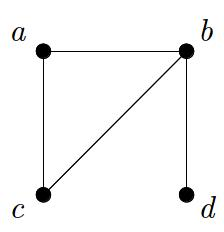
\includegraphics[scale=0.5]{GraphExample}
\caption{\label{fig:Graph-Example}An Example of Graph}
\end{figure}

If $v$ is an endpoint of and edge $e$, then we say that $e$ is is \emph{incident}\index{Incident edge} on $v$. The \emph{degree}\index{Degree of a vertex} of a vertex $v$, written $\deg(v)$, is equal to the number of edges which are incident on $v$. A vertex of degree zero is called \emph{isolated}\index{Isolated vertex}; a vertex of degree one is called \emph{pendant}\index{Pendant vertex}. The \emph{neighborhood}\index{Neighborhood of a vertex} of vertex $v$, denoted by $N(v)$, is the set of all vertices that are adjacent to $v$. If $A \subset V$, the neighborhood of $A$ is $N(A) = \cup_{v \in A} N(v)$. A \emph{path}\index{Path} in a graph is a sequence of distinct vertices $\{v_{0}, v_{1}, \ldots ,v_{k}\}$ in which $v_{i}$ and $v_{i+1}$ are adjacent for each $1 \leq i < k$. A path is a \emph{simple path}\index{Simple path} if it does not repeat any node. A graph is \emph{connected}\index{Connected graph} if every two nodes have a path between them. If $v_{0} = v_{k}$ we say that the path is a \emph{cycle}\index{Cycle}. A cycle is a \emph{simple cycle}\index{Simple cycle} if it contains at least three nodes and repeats only the first and last nodes. 

\begin{example}
Given a graph $G=(V,E)$, the \emph{handshaking theorem}\index{Handshaking theorem} states that $\sum_{v \in V} deg(v) = 2 m$, where $m = d(E)$, since each edge has two end points.
\end{example}

If the pairs of vertices $u, v$ are ordered pairs, the graph is called \emph{directed graph}\index{Directed graph}, and in that case, $u$ is called the \emph{initial vertex}\index{Initial vertex} and $v$ the \emph{terminal vertex}\index{Terminal vertex}. If $G$ is directed graph, we call the \emph{in-degree}\index{In-degree of a vertex} of a vertex $v$, denoted by $indeg(v)$, to the number of edges in which $v$ is an terminal vertex, and \emph{out-degree}\index{Out-degree of a vertex}, denoted by $outdeg(v)$, to the number of edges in which $v$ is an initial vertex. A directed grap is \emph{strongly connected}\index{Strongly connected graph} is a direct path connects every two nodes. Directed graphs are depiced using arrows instead of lines to represent edges.

A graph $G$ is said to be \emph{bipartite}\index{Bipartite graph} if the set of vertices $V$ can be partitioned into two subsets $V_1$ and $V_2$ such that each edge of $G$ connects a vertex of $V_1$ to a vertex of $V_2$. Bipartite graphs are usually denoted by $G=(V_1, V_2, E)$. The degree of the vertices of a bipartite graph satisfied the following property, called the \emph{degree sum formula}\index{Degree sum formula}, $\sum_{u \in V_1} deg(u) = \sum_{v \in V_2} deg(v) = d(E)$.

A graph $G(V',E')$ is a \emph{subgraph}\index{Subgraph} of $G(V,E)$ if $V'$ is a subset of $V$ and $E'$ is a subset of $E$ whose endpoints belong to $V'$. A graph $G$ is called a \emph{labeled graph}\index{Labeled graph} if its edges and/or vertices are assigned data of one kind or another. In particular, if each edge $e$ of $G$ is assigned a nonnegative number $w(e)$ then $w(e)$ is called the \emph{weight}\index{Weight of an edge} of $e$.

A particular type of graph that will be extensively used in this book are trees. A \emph{tree}\index{Tree} is a non-empty graph in which any two vertices are connected by a unique path. Given a tree, we will always designate a particular vertex, called the \emph{root}\index{Root of a tree} of the tree, and direct each edge away from that root.

\begin{example}
An equivalent definition of trees is provided by set theory. According to set theory a tree is a partially ordered set $(T, <)$ such that for each $t \in T$, the set $S = \{ s \in T : s < t \}$ has an element that is smaller than every other element of S (\emph{least element}).
\end{example}

Let $T$ be a tree. If $v$ is a vertex in $T$ other than the root, the \emph{parent}\index{Parent of a vertex} of $v$ is the unique vertex $u$ such that there is an edge connecting $u$ to $v$. If $u$ is the parent of $v$, then $v$ is called a \emph{child}\index{Child of a vertex} of $u$. A \emph{sibling}\index{Sibling to a vertex} to a vertex $v$ is any other vertex on the tree which has the same parent than $v$. The \emph{ancestors}\index{Ancestors of a vertex} of a vertex are the vertices in the path from the root to this vertex, excluding the vertex itself and including the root. The \emph{descendants}\index{Descendant of a vertex} of a vertex $v$ are those vertices that have $v$ as an ancestor. A vertex is called a \emph{leaf}\index{Leaf vertex} if it has no children. Vertices that have children are called \emph{branches}\index{Branches of a tree}. The \emph{depth}\index{Depth of a vertex} of a vertex $v$ is the length of the unique path from the root to $v$. The \emph{height}\index{Height of a tree} of a tree is the maximum of the levels of its vertices. 

\begin{example}
The following applies to the tree depicted in Figure \ref{fig:BinaryTree-Example}: the root is the vertex $a$; $c$ is a parent of $d$ and $d$ is a child of $c$; $d$ and $g$ are siblings; the ancestors of $d$ are $a$ and $c$; the descendants of $c$ are $e$, $e$ and $f$; $b$, $e$, $f$ and $g$ are leaf nodes; $c$ and $d$ are branches; the depth of $d$ is 3; the height of the tree is 4.
\end{example}

\begin{figure}[h]
\centering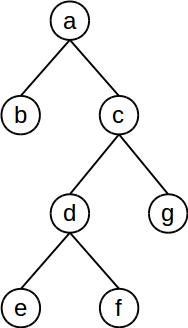
\includegraphics[scale=0.5]{BinaryTree}
\caption{\label{fig:BinaryTree-Example}An Example of Tree}
\end{figure}

If $v$ is a vertex in a tree, the \emph{subtree}\index{Subtree} with $v$ as root is the subgraph of the tree consisting of $v$ and its descendants and all edges incident to these descendants. A tree is called an \emph{k-ary tree}\index{k-ary tree} if every branch has not more than $k$ children. The tree is called a \emph{full k-ary tree}\index{full k-ary tree} if every branch has exactly $k$ children. An \emph{k-ary} tree with $k=2$ is called a \emph{binary tree}\index{Binary tree}. A $k$-ary tree of height $h$ is \emph{balanced}\index{Balanced tree} if all its leaves are have a depth of $h$ or $h-1$.

\begin{example}
A tree with $n$ vertices has $n-1$ edges. A full $k$-ary tree with $i$ branches contains $m=ki+1$ vertices.
\end{example}

\emph{Tree traversal}\index{Tree traversal} is the process of visiting each node in a tree exactly once. Tree traversals are classified by the order in which the nodes are visited, having \emph{depth-first} and \emph{breadth-first} order. In depth-first traversal\index{Depth-first tree traversal}, the algorithm starts at the root node and explores as far as possible along each branch before going to the next sibling. There are three common ways process the nodes in the tree: \emph{in-order}\index{Post-order tree traversal}, \emph{pre-order}\index{Post-order tree traversal} and \emph{post-order}\index{Post-order tree traversal}.

The following C-like code will print a tree using a recursive pre-order depth-first traversal algorithm:

\begin{verbatim}
    void print_tree(binary_tree *tree) {
        if (!is_empty(tree)) {
            printf("%c\n",tree->node); /* print node */
            print_tree(tree->left_branch); /* process left branch */
            print_tree(tree->right_branch); /* process right branch */
        }
    }
\end{verbatim}

In breadth-first traversal\index{Depth-first tree traversal}, the algorithm starts at the tree root and explores all nodes at the present depth before going to the next depth level. Depth-first tree traversal alogorithms require the use of advanced data structures. Please refer to the references section for an example of such algorithms.

\begin{example}
A pre-order depth-first traversal of the tree depicted in Example \ref{ex:binary_tree} will produce the following string "abcdefg". A pre-order breadth-first traversal will print "abcdgef".
\end{example}

%
% Section: Counting Methods
%

\section{Counting Methods}
\label{sec:counting}

\emph{Combinatorics}\index{Combinatorics} is the branch of mathematics that deals with the study of discrete objects and the relationships between them. It is concerned with counting, arranging, and selecting objects, along with the methods used to accomplish these tasks. Combinatorics offers powerful tools for managing vast collections of objects that possess specific properties. In this section, we will review the most important results of combinatorics from the point of view of sets and ordered lists.

The \emph{multiplication rule}\index{Multiplication rule} refers to a fundamental principle that governs the number of possible outcomes in the Cartesian product of sets. According to this rule, if we have $k$ sets $A_1, A_2, \ldots, A_k$, and each sets has $k_i$ elements $\left( i=1, \ldots, k \right)$, then the cartesian product $A_1 \times A_2 \times \ldots \times A_k$ has a total number of $n_1 n_2 \ldots n_k$ elements. In particular, if the set $A$ has $n$ elements, then $A^k$ has $n^k$ elements.

The \emph{inclusion–exclusion principle}\index{Inclusion-exclusion principle} computes the size of the union of multiple sets, given the size of each set, and the size of each possible intersection of the sets. If we have $k$ sets $A_1, A_2, \ldots, A_k$, then 
\begin{equation*}
\begin{split}
d \left( \bigcup_{i=1}^k A_i \right) & = \sum_{i=1}^k d \left( A_i \right) - \sum_{i<j} d \left( A_i \cap A_j \right) + \sum_{i<j<l} d \left( A_i \cap A_j \cap A_l \right) - \\
& - \sum_{i<j<l<m} d \left( A_i \cap A_j \cap A_l \cap A_m \right) + \ldots +  (-1)^{k+1} d \left( A_1 \cap A_2 \cap \ldots \cap A_k \right) 
\end{split}
\end{equation*}
\emph{Permutations}\index{Permutations} count the number of ways we can arrange the elements of a set. Let $A$ be a set with $n$ elements, the number of permutations of $n$ elements taken $k$ at a time, denoted by $P_{n,k}$, is given by $P_{n,k} = n \left( n-1 \right) \ldots \left( n-k+1 \right)$. When $k=n$, the number of permutations is given by $P_{n,n} = n \left( n-1 \right) \cdots 1=n!$, where the symbol $n!$ is read $n$ factorial.

For very large computations, it is uselful to use the following approximation of $n!$, called \emph{Stirling's formula}:
\[
\log\left(n!\right) \approx \frac{1}{2}\log\left(2\pi\right)+\left(n+\frac{1}{2}\right)\log\left(n\right)-n
\]

\begin{example}
Given the set \{a, b, c \}, there are six possible permutations for its selements: $[a, b, c], [a, c, b], [b, a, c], [b, c, a], [c, a, b], [c, b, a]$. Each permutation is a different ordering of the elements in the original set.
\end{example}

Many problems of counting deal with the number of subsets of a certain size that are contained in a fixed set. If a set has $n$ elements, there are $2^n$ possible subsets, including the empty set and the set itself. The number of subsets of size $k$, called the number of \emph{combinations}\index{Combinations} of $k$ elements from a set of $n$, and denoted by $C_{n,k}$, is calculated using the formula $C_{n,k}=\frac{P_{n,k}}{k!}=\frac{n!}{k!\left(n-k\right)!}$. The number $C_{n,k}$ is also denoted by the symbol ${n \choose k}$, and called \emph{binomial coefficient}\index{Binomial coefficient}. We have that for all $n$, ${n \choose 0}={n \choose n}=1$, , for all n and all $k=0,1,\ldots,n$, ${n \choose k}={n \choose n-k}$, and ${n \choose k} = 0$ for $k>n$.

\begin{example}
Given the set $\{a, b, c, d \}$, there are a total of 4 combinations of size 3: $[a, b, c]$, $[a, b, d]$, $[a, c, d]$, and $[b, c, d]$. The order does not matter in combinations, so for example $[a, c, d]$ and $[d, c, a]$ are considered to be the same combination.
\end{example}

The \emph{multinomial coefficient}\index{Multinomial coefficient} is a generalization of the binomial coefficient to more than two categories or types. It represents the number of ways to partition a set of objects into a fixed number of subsets, with each subset containing a specified number of objects. Suppose we have a set with $n$ elements, which can be partitioned into $k$ subsets of sizes $n_1, n_2, \ldots, n_k$, respectively. The multinomial coefficient, denoted by the symbol ${n \choose n_{1},n_{2},\ldots,n_{k}}$, represents the number of possible partitions, and is given by ${n \choose n_{1},n_{2},\ldots,n_{k}} = \frac{n!}{n_{1}!n_{2}!\ldots n_{k}!}$.

\section*{References}

An easy to read book on discrete mathematics that cover what it is covered in this chapter and part of the the following chapters is \cite{johnsonbaugh2009discrete}. For more information about formal languages we recommend \cite{sipser2012introduction}. And for a book on algorithms, and in particular, algorithms to deal with graphs and trees, we recommend \cite{cormen1990introduction}.


%
% CHAPTER: Probability Theory
%

%
% CHAPTER: Probability Theory
%

\chapterimage{Koenigsberg_Map_by_Bering_1613.pdf} % Chapter heading image

\chapter{Discrete Probability}
\label{chap:Probability Theory}

\begin{quote}
\begin{flushright}
\emph{Mathematics may be defined as the subject in which\\
we never know what we are talking about,\\
nor whether what we are saying is true.}\\
Bertrand Russell
\end{flushright}
\end{quote}
\bigskip

{\color{red} Introduce the chapter}

%
% Section: Foundations
%

\section{Foundations}
\label{sec:probability_foundations}

\emph{Probability} is a very difficult concept to grasp. Imagine we throw a dice and we want to calculate the probability that the number that appears is even. The dice has six possible outcomes, and since there are three even numbers, we say that the probability of having an even number is $3/6$ or $1/2$. This what the \emph{classical interpretation}\index{Classical interpretation of probability} of probability proposes: if we have an experiment in which all the possible outcomes are equally likely to happen, the probability of an event is the number of favourables cases divided by the total number of cases. The problem with this interpretations is that "equally likely" is essentially the same thing than "having the same probability", and so, it is a circular definition. An alternative approach to assign probabilities would be to apply the \emph{principle of indiference}\index{Principle of indiference}: in absense of any relevant evidence, all possible outcomes should have the same probability. The problem with this principle araises when there is evidence that not all cases are equal. For example, what happens if we know that the dice is loaded?, how do we assign probabilities when not all the sides are equally likely?

The \emph{frequentist interpretation}\index{Frequentist interpretation of probability} of probability proposes throwing the dice multiple times and calculating the releative frequency of even numbers with respect to the total number of throws. The general idea is to repeat the experiment a sufficiently large number of times under similar conditions and assing the releative frequency of each outcome as its probability. This interpretation has two main limitations. First of all, it is not clear how we should repeat an experiment under "similar conditions", since if we use exactly the same conditions the results of all the trials would be the same. The second is that it is not defined what a "large number of times" means (technically speaking, we should repeat the experiment an infinite number of times). From a practical point of view it is very difficult to apply the frequentist interpretation: some experiments cannot be repeated a large number of times, for example, what it is the probability that a candidate wins an election?; probability is defined in terms of a succession of experiments, so we cannot compute the probability of an individual outcome; and we require that the relative frequency limit exists, that is not always the case, for example, in finacial time series.

A third intepreation of the concept of probability, called \emph{subjective interpretation}\index{Subjective interpretation of probability}, proposes to assign to each event a probability based on our degree of belief: the more we belive that an event is true, the higher its probability. Of course, not all possible combinations of probabilities are valid, it is required that some rules of coherence must be satisfied. For example, if we are betting on the result of the dice thrown, an assigment of probabilities that guarantees that we will loose all of our money (what it is called a \emph{dutch book}\index{Dutch book}) does not satify the conditions of the subjective interpretation. It turns out that the conditions neccesary and sufficient to guarantee a fair bet are the same conditions required by the axioms of probability introduced below. In this sense, we can assign to events whatever probabilities we want, as long as they are consistant with the axioms of probability. The problem with the subjective interpretation is that people have different degrees of belief. A solution to this problem is proposed by the \emph{Bayesian interpretation}\index{Bayesian interpretation of probability} of probability: we start with a tentative assigment of probabilities, and as we get futher evidence, we modify our degree of belief, or probability, accordingly; as we get more evidence, estimated probabilities will converge to the true probabilities. In any case, assigning probabilities to an infinite number of events is not, in general, human attainable. 

Currently, the concept of probabilty is defined axiomatically (\emph{axiomatic interpretation}\index{Axiomatic interpretation of probability}), which means we give up in trying to define what a probability is, and instead we assume as true some of its properties. Intuitively, a probability should be a number between $0$ and $1$, where an event that cannot happen has a probability of zero, and an event that for sure will happen has a probability of one. That fact that probability must be a number between $0$ and $1$ is more a social convention that a real mathematical requirement, since other ranges of numbers are equally good. We require some additional properties of probabilities. For example, if two events $A$ and $B$, with probabilities $P \left( A \right)$ and $P \left( B \right)$ respectively, cannot happen at the same time, the probabilty that either $A$ or $B$ occurs should be $P \left( A \right) + P \left( B \right)$. If $A$ and $B$ can happen at the same time, but they are not related in any way, that is, they are independent events (whatever that means), we expect that the probability of the two events happening at the same time shold be $P \left( A \right) P \left( B \right)$. Finally, we are also interested in the pobabily of $A$ happeing assuming that $B$ has already happend, it should be the the fraction of probability $A$ that intersects with $B$. Probability, then, would be anything that satisfies these properties. The problem with the axiomatic interpretation is that too many things satisfy those requirements, like for example phisical quantities like normalized mass or normalized volume.

Probability theory is about assigning a number to some events from a sample space. The word "event" is a little bit misleading in this context because it suggests that something happened, which is not always the case. However, to avoid confusion, we will keep calling events to what are essentially subsets.

\begin{definition}
Let $\left( \Omega, \mathcal{A} \right)$ be a field over a non-empty discrete set. We call $\Omega$ the \emph{sample space}\index{Sample space}, its elements \emph{outcomes}\index{Outcome}, and the elements of $\mathcal{A}$ events. In particular, we call $\Omega$ the \emph{certain event}\index{Certain event} and $\varnothing$ the \emph{impossible event}\index{Impossible event}.
\end{definition}

As we saw in Section \ref{sec:sets}, given that $\left( \Omega, \mathcal{A} \right)$ is a field, we have that $\Omega \in \mathcal{A}$ and that $\varnothing \in \mathcal{A}$. Moreover, the union of a finite collection of events is an event $A_1 \cup A_2 \cup \ldots \cup A_n \in \mathcal{A}$, and that the intersection of a fine collection of events is also an event $A_1 \cap A_2 \cap \ldots \cap A_n \in \mathcal{A}$.

As we have said in the previous chapter, our main interest is in discrete mathematics, and so, we will mostly working with probabilities over discrete (finite or countably infinite) sets. An extension of the concept of probability to continuous sets requires the use of $\sigma$-algebras\index{$\sigma$-algebra} of sets instead of fields and the use measure theory.

The standard axiomaitization used in probability theory are the \emph{Kolmogorov axioms}\index{Kolmogorov axioms}.

\begin{definition}
A \emph{probability}\index{Probability} is a real number $P(A) \in \mathbb{R}$ assigned to each event $A \in \mathcal{A}$ of the field $\left( \Omega, \mathcal{A} \right)$, that satisfy the following axioms:

\medskip

\begin{description}
\item [Axiom 1] $P(A) \geq 0$.
\item [Axiom 2] $P(\Omega) = 1$.
\item [Axiom 3] For every finite sequence of disjoint events $A_1, A_2, \ldots, A_n$ we have that $P(\cup_{i=1}^n) = \sum_{i=1}^n P(A_i)$.
\end{description}
\end{definition}

A problem with these axioms is that they cannot be reduced to first-order logic (See Appendix \ref{apx:foundations_mathematics}), since real numbers cannot be described in terms of first-order logic. Also, no information is contained in the axioms about how probabilites can be assigned to events.

\begin{example}
Let $\Omega$ a sample space containing $n$ elements equally probable. If $A \subset \Omega$ is an event with $d(A) = m$, the we have that $P(A) = m/n$.
\end{example}

Let's prove some basic results of probabilities, starting by calculating the probability of the complement of an event, that is, the probability that this event does not happen.

\begin{proposition}
For every event $A$, $P \left( A^{c} \right) = 1 - P \left( A \right)$
\end{proposition}
\begin{proof}
The sets $A$ and $A^c$ are disjoint and $A \cup A^c = \Omega$. Given Axiom 3 we have that $P \left( A \cup A^c \right) = P \left( A \right) + P \left( A^c \right)$, and given Axiom 2 we have that $P \left( A \cup A^c \right) = P(\Omega) = 1$, and so, $P \left( A \right) + P \left( A^c \right) = 1$.
\end{proof}

As a direct consequence of previous proposition, we can derive the probability of the impossible event.

\begin{proposition}
The probability of the impossible event is zero, that is, $P \left( \varnothing \right) = 0$
\end{proposition}
\begin{proof}
Given that $P \left( \varnothing \right) = 1 - P \left( \Omega \right) = 0$
\end{proof}

As expected, sub-events have smaller probabilities than events.

\begin{proposition}
If $A\subset B$ then $P \left( A \right) \leq P \left( B \right)$
\end{proposition}
\begin{proof}
The event $B$ can be decomposed as the union of two disjoint events $A$ and $A^c \cap B$, so we have that $P \left( B \right) = P \left( A \right) + P \left( A^c \cap B \right)$, that combined with the fact that  $P \left( A^c \cap B \right) \geq 0$ proves the proposition.
\end{proof}

We have in place all the elements we need to prove that probabilities are numbers between zero and one.

\begin{proposition}
For every event $A$ we have that $0 \leq P \left( A \right) \leq 1$.
\end{proposition}
\begin{proof}
Based on Axiom 1 and given that $A \subset \Omega$ and so $P \left( A \right) \leq P \left( \Omega \right) = 1$
\end{proof}

Axiom 3 allows us to compute the probability of the union of disjoint events. Next proposition allows us to compute the probability of the union of events that are not disjoint.

\begin{proposition}
For every two events $A$ and $B$, $Pr\left(A\cup B\right)=Pr\left(A\right)+Pr\left(B\right)-Pr\left(A\cap B\right)$.
\end{proposition}
\begin{proof}
The union of sets $A$ and $B$ can be decomposed as the union of the two disjoint sets $A \cup B = B \cup \left( A \cap B^c \right)$, so given Axiom 3 we have that
\[
P \left( A \cup B \right) = P \left( B \right) + P \left( A \cap B^c \right)
\]
In the same way, the set $A$ can be decomposed as the unition of the disjoint sets $A = \left( A \cap B \right) \cup \left( A \cap B^c \right)$, so that
\[
P \left( A \cup B^c \right) = P \left( A \right) - P \left( A \cap B \right)
\]
Combining boths expression we get the desired result.
\end{proof}

The follwoing formula is a generalization to the case of $n$ events $A_1, \ldots, A_n$:
\begin{multline}
P \left( \bigcup_{i=1}^n A_i \right) = \sum_{i=1}^n P \left( A_i \right) - \sum_{i<j} P \left( A_i \cap A_j \right) + \sum_{i<j<k} P \left( A_i \cap A_j \cap A_k \right) - \\
 - \sum_{i<j<k<l} P \left( A_i \cap A_j \cap A_k \cap A_l \right) + \ldots +  (-1)^{n+1} P \left( A_1 \cap A_2 \cap \ldots \cap A_n \right) 
\end{multline}

%
% Section: Conditional Probability
%

\section{Conditional Probability}
\label{sec:probability_conditional}

The concept of conditional probability plays a fundamental role in the area of statistical learning. Traditionally, the conditional probability of event $A$ given event $B$ has been seen as the updated probability of $A$ after we have learnt that $B$ has occurred. However, this interpretation suggests that there is a causal relationshipt between events $B$ and $A$, which is not necessarly true.

Based on Kolmogorov's axioms, conditional probability is defined as a quotient.

\begin{definition}
Let $A$ and $B$ two events such that $P \left( B \right) \neq 0$. The \emph{conditional probability} of $A$ given $B$, denoted by $P \left( A \mid B \right)$, is defined as
\[
P\left(A\mid B\right) = \frac{P\left(A\cap B\right)}{P\left(B\right)}
\]
\end{definition}

Conditional probability is itself a probability, since it satisfy the axioms. Conditional probability $P\left(A\mid B\right)$ is not defined if $P\left(B\right)=0$.

The probability that two events will happen toghether (although not necessarily at the same time), given their conditional probabilities, is $P \left( A \cap B \right) = P \left( A \mid B \right) P \left( B \right)$ or $P \left( A \cap B \right) = P \left( A \mid B \right) P \left( B \right)$. The formula $P \left( A \cap B \right) = P \left( A \mid B \right) P \left( B \right)$ provides a more intuitive interpretation of the concept of conditional probability. There are even some authors that have created alternative axiomatizations of probability in which this property is one of the assumed axioms.

The generalation of this formula for the case of $n$ events, called \emph{multiplication rule}, is $P \left( A_{1} \cap A_{2} \cap \ldots \cap A_{n} \right) = P \left( A_{1} \right) P \left( A_{2} \mid A_{1}\right) \ldots  P \left( A_{n} \mid A_{1}\cap A_{2} \cap \ldots \cap A_{n-1} \right)$.

The concept of events independence plays also a very important role in probability theory and statistical learning. 

\begin{definition}
Two events $A$ and $B$ are said to be \emph{independent} if $P \left( A \cap B \right) = P \left( A \right) P \left(B \right)$
\end{definition}

From an intuitive point of view, the events $A$ and $B$ are independent if observing that B has occurred does not alter the probability of A. This property can be derived from the definition of independence.

\begin{proposition}
Let $A$ and $B$ two events shuch that $P \left( A \right) > 0$ and $P \left( B \right)>0$, then $A$ and $B$ are independent if and only if $P \left( A \mid B\right) = P \left( A \right)$ and $P \left( B \mid  A \right) = P \left( B \right)$.
\end{proposition}
\begin{proof}
Assume that $A$ and $B$ are independent, that is $P \left( A \cap B \right) = P \left( A \right) P \left(B \right)$, then
\[
P \left( A \mid B \right) = \frac{P\left(A\cap B\right)}{P\left(B\right)} = \frac{P \left( A \right) P \left(B \right)}{P\left(B\right)} = P \left( A \right)
\]
Now let's assume that $P \left( A \mid B \right) = P \left( A \right)$. Given the multiplication rule we have that,
\[
P \left( A \cap B \right) =  P \left( A \mid B \right) P \left( B \right) = P \left( A \right) P \left( B \right)
\] 
The same applies if we interchange $A$ and $B$. 
\end{proof}

As it was the case of conditional probability, some authors claim that independence, being a fundamental concept in probability theory, should be assumed as an axiom, not as a definition.

The concept of independence can be generalized to the case of multiple events: the events $A_{1}, \ldots, A_{n}$ are independents (or mutually independent) if for every subset $A_{i_1}, \ldots, A_{i_j}$ composed by $j$ events $\left( j = 2, 3, \ldots, n \right)$, we have that $P \left( A_{i_1} \cap \ldots \cap A_{i_j} \right) = P \left( A_{i_1} \right) \ldots P \left( A_{i_j}\right)$.

There is some confussion about the difference between mutually exclusive, or disjoint, events and independent events. If $A$ and $B$ are two mutually exclusive events, it does not make too much sense to compute the probability that $A$ will happen given $B$, since if $B$ happens, $A$ cannot happen; in the same way that it does not make too much sense to talk about the conditional probability that $A$ will happen given $B$ if the probability of $B$ is zero.

A particular interesting case is when events $A$ and $B$ are not independent but they become independent if we know that some other even $C$ has happened. 

\begin{definition}
Let's $A$, $B$ and $C$ events such that $P\left( B \cap C \right)>0$. $A$ and $B$ are \emph{conditionally independent} given $C$ if $P\left(A \mid B \cap C \right) = P\left( A \mid C \right)$.
\end{definition}

Baye's theorem provides the foundations of Bayesian inference (see Section {\color{red} XX}), a very important technique in the area of statistical learning.

\begin{theorem} (Bayes' Theorem) Let's $A$ and $B$ two events such that $P\left( B \right) \neq 0$. Then we have that
\[
P \left( A \mid B \right) = \frac{P \left( B \mid A \right) P \left( A \right)}{P \left( B \right)}
\]
\end{theorem}
\begin{proof}
\end{proof}

\begin{example}
Let $E$ a disease that affects to one of every one million persons, $P(E) = 1 \times 10^{-6}$, and let $+$ a test designed to detect the disease that fails once every one thousand applications, $P(+ \mid E) = 999/1000$. We are interested in knowing the probability of having the disease if the test is positive $P(E \mid +)$. Applying Bayes' theorem we have that:
\[
P(E \mid +) = \frac{P(+ \mid E) P(E)}{P(+)} = \frac{P(+ \mid E) P(E)}{P(+ \mid E) P(E) + P(+ \mid E^c) P(E^c)} = 0.001
\]
That is, although the test only fails once per thousand applications, it is still very unlikely we have the disease in the case of a positive result. This counterintuitive result is explained because the probability of failure of the test $10^{-3}$ is much higher than the probability of having the disease $10^{-6}$. In practice we solve this problem by applying a second test to those who got a positive result, since the probability of having the disease after two positives is $0.5$ (assuming that the successive repetitions of the test are independent).
\end{example}

The probability $P\left( B \right)$ is called \emph{prior probability}, and $P\left( B\mid A \right)$ is called \emph{posterior probability}.

%
% Section: Random Variables
%

\section{Random Variables}
\label{sec:probability_random_variables}

{\color{red} Say something intelligent here}

% Random Variables and Discrete Distributions

\subsection{Random Variables and Discrete Distributions}

{\color{red} Definition of Random Variable}

{\color{red} Introduce the concept of random variable}

\begin{definition}
Let $\Omega$ be the sample space for an experiment. A random variable is a real-valued function $X : \Omega \rightarrow \mathbb{R}$, where the probability of having the value $x \in \mathbb{R}$, denoted by $P(X=x)$, is given by $P(\{ \omega \in \Omega : X(\omega) = x\})$.
\end{definition}

{\color{red} Eplain why "random variable" is a terrible name}

{\color{red} Am I right about the interpretation of the concept of random variable?}

{\color{red} Introduce the concept of probability distribution. Recall we are only considering discrete distributions.}

\begin{definition}
Let $X$ be a random variable. The distribution of $X$ is the collection of all probabilities of the form $P\left(X\in C\right)$ for all sets $C$ of the real numbers such that $\left\{ X\in C\right\}$  is an event. The Distribution of a Random Variable. Let $C$ be a subset of the real line such that $\left\{ X\in C\right\}$  is an event, and let $P\left(X\in C\right)$ denote the probability that the value of $X$ will belong to the subset $C$, then $P\left(X\in C\right)=P\left(\left\{ s\,:\,X\left(s\right)\in C\right\} \right)$

The \emph{probability mass function}\index{Probability mass function} of a discrete random variable $X$ with range $\{ x_1, x_2, \ldots, x_i, \ldots \}$ is defined as the function $f$ such that $f(x_i) = P(X=x_i)$.
\end{definition}

{\color{red} The distribution of $X$ is itself a probability measure on the set of real numbers.}

{\color{red} Is it too early for this?} A \emph{parametric random variable} $X$, denoted by $f\left(X \mid \theta \right)$, is a distribution that belongs to a family of functions parameterized by $\theta$, where $\theta$ can be a single parameter, or a vector of several parameters. 

{\color{red} If a random variable $X$ has a discrete distribution, the probability function (abbreviated p.f.) of $X$ is defined as the function $f$ such that for every real number $x$, $f\left(x\right)=P\left(X=x\right)$}

\begin{example}
A random variable $Z$ that takes only two values $0$ and $1$ with $P\left(Z=1\right)=p$ has the Bernoulli distribution with parameter $p$. We also say that $Z$ is a Bernoulli random variable with parameter $p$.
\end{example}

{\color{red} The closure of the set $\left\{ x\,:\,f\left(x\right)>0\right\}$  is called the support of (the distribution of) $X$. Probability functions are also known as probability mass functions (p.m.f.).}

{\color{red} Introduce the following proposition}

\begin{proposition}
Let $X$ be a discrete random variable with p.f. $f$. If $x$ is not one of the possible values of $X$, then $f\left(x\right)=0$. Also, if the sequence $x_{1},x_{2},\ldots$ includes all the possible values of $X$, then $\sum_{i=1}^{\infty}f\left(x_{1}\right)=1$.
\end{proposition}
\begin{proof}
\end{proof}

{\color{red} The p.f. of a discrete random variable characterizes its distribution.}

\begin{proposition}
If $X$ has a discrete distribution, the probability of each subset $C$ of the real line can be determined from the relation $P\left(X\in C\right)=\sum_{x_{i}\in C}f\left(x_{i}\right)$
\end{proposition}
\begin{proof}
\end{proof}

{\color{red} Uniform Distribution on Integers}

\begin{definition}
Let $a \leq b$ be integers. Suppose that the value of a random variable $X$ is equally likely to be each of the integers $a, \ldots, b$. Then we say that $X$ has the uniform distribution on the integers $a, \ldots, b$.
\end{definition}

{\color{red} Introduce the following propostion}

\begin{proposition}
If $X$ has the uniform distribution on the integers $a,\ldots,b$, the p.f. of $X$ is $f\left(x\right)=\begin{cases}
\frac{1}{b-a+1} & for\,x=a,\ldots,b\\
0 & otherwise
\end{cases}$
\end{proposition}
\begin{proof}
\end{proof}

{\color{red} The uniform distribution on the integers $a, \ldots, b$ represents the outcome of an experiment that is often described by saying that one of the integers $a, \ldots, b$ is chosen at random. A uniform distribution cannot be assigned to an infinite sequence of possible values}

{\color{red} Random variables can have the same distribution without being the same random variable. (this is also mentioned in the masures of centrality section}.

Binomial Distributions

\begin{example}
Suppose we perform $N$ independent trials where each trial either succeeds or fails with probability of success $p$, and let $X$ the random variable defined by the number of successes. The probability of having exactly $n$ successes $P(X=n)$ follows a \emph{binomial distribution} with parameters $N, p$, defined by:
\[
f(n\mid N, p) = \binom{N}{n} p^n (1-p)^{(N-n)}
\]
\end{example}

\begin{definition}
The discrete distribution represented by the p.f.f $\left(x\right)=\begin{cases}
{n \choose x}p^{x}\left(1-p\right)^{n-x} & for\,x=0,1,\ldots,n\\
0 & otherwise
\end{cases}$
\end{definition}

{\color{red} is called the binomial distribution with parameters $n$ and $p$.}

{\color{red} Consider a general experiment that consists of observing $n$ independent trials with only two possible results for each trial: success and failure. Then the distribution of the number of trials that result in success will be binomial with parameters $n$ and $p$, where $p$ is the probability of success on each trial.} 

The Cumulative Distribution Function

{\color{red} Introduce the concept of random sample}

The concept of random sample plays a very important role in the area of statistical learning. Assuming that a collection of random variables form a random sample simplifies the mathematics behind inference methods. However, the requirements behind random samples are not always satisfied in practice.

\begin{definition}
Let $f$ be a probability distribution, and let $X_1, X_2, \ldots, X_n$ be $n$ random variables. It is said that the variables $X_1, X_2, \ldots, X_n$ form a \emph{random sample} for the distribution $f$ if they are independent, and the marginal distribution of each of them is $f$. 
\end{definition}

If the random variables $X_1, X_2, \ldots, X_n$ form a random sample for the distribution $f$, it is said that they are \emph{independent and identically distributed}, abbreviated \emph{i.i.d}. The number $n$ is called the \emph{sample size}. The joint distribution $g$ of the random sample is given by:
\[
g \left( x_1, x_2, \ldots, x_n \right) = f \left( x_1 \right) f \left( x_2 \right) \ldots f \left( x_n \right)
\]
for all the points $\left( x_1, x_2, \ldots, x_n \right) \in \mathcal{R}$.

% Bivariate Distributions

\subsection{Bivariate Distributions}

\begin{definition}
Let $X$ and $Y$ be random variables. The joint distribution or bivariate distribution of $X$ and $Y$ is the collection of all probabilities of the form $Pr\left[\left(X,Y\right)\in C\right]$ for all sets $C$ of pairs of real numbers such that $\left[\left(X,Y\right)\in C\right]$ is an event.
\end{definition}

{\color{red} This joint distribution is itself a probability measure on the set of ordered pairs of real numbers.}

\begin{proposition}
Suppose that two random variables $X$ and $Y$ each have a discrete distribution. Then $X$ and $Y$ have a discrete joint distribution.
\end{proposition}

\begin{definition}
The joint probability function, or the joint p.f of $X$ and $Y$ is defined as the function f such that for every point $\left(x,y\right)$ in the $xy$-plane $f\left(x,y\right)=Pr\left[X=x\enskip and\enskip Y=y\right]$
\end{definition}

\begin{proposition}
Let $X$ and $Y$ have a discrete joint distribution. If $\left(x,y\right)$ is not one of the possible values of the pair $\left(X,Y\right)$, then $f\left(x,y\right)=0$. Also, $\sum_{\left(x,y\right)}f\left(x,y\right)=1$
\end{proposition}

Finally, for each $C$ of ordered pairs $Pr\left[\left(X,Y\right)\in C\right]=\sum_{\left(x,y\right)\in C}f\left(x,y\right)$

{\color{red} Any function that satisfied the two displayed formulas is the joint p.d.f. for some probability distribution.}

A particular interesting case of bivariate distribution is given by the sum of two random variables. This is a highly confusing scenario, since we are not adding two probability distributions, as the notation $X + Y$ might suggest. Instead, we are defining a new random variable over the cartesian product of the original sample spaces.

\begin{definition}
Let $X : \Omega_X \rightarrow \mathbb{R}$ and $Y : \Omega_Y \rightarrow \mathbb{R}$ be two random variables. The sum distribution of $X$ and $Y$, denoted by $X + Y$, is defined as the random variable $X + Y : \Omega_X \times \Omega_Y \rightarrow \mathbb{R}$ that assigns to each pair $\left( a, b \right) \in \Omega_X \times \Omega_Y$ the number $X(a) + Y(b)$.
\end{definition}

% Marginal Distribution

\section{Marginal Distribution}

{\color{red} Often, we start with a joint distribution of two random variables and we then want to find the distribution of just one of them, called the marginal distribution.}

\begin{definition}
Suppose that $X$ and $Y$ have a joint distribution. The c.d.f. of $X$ derived with the above theorem is called the marginal c.d.f. of $X$. Similarly, the p.f. or p.d.f. of $X$ associated with the marginal c.d.f. of $X$ is caled the marginal p.f. or marginal p.d.f. of $X$.
\end{definition}

\begin{proposition}
If $X$ and $Y$ have a discrete joint distribution for which the joint p.f. is f, then the marginal p.f. of $X$ is $f_{1}\left(x\right)=\sum_{y}f\left(x,y\right)$
\end{proposition}
\begin{proof}
\end{proof}

{\color{red} Similarly, the marginal p.f. $f_{2}$ of $Y$ is $f_{2} \left(y\right)=\sum_{x}f\left(x,y\right)$.}

{\color{red} Although the marginal distributions of X and Y can be derived from their joint distribution, it is not possible to reconstruct the joint distribution of X and Y from their marginal distributions without additional information.}

{\color{red} Independent Random Variables}

\begin{definition}
It is said that two random variables $X$ and $Y$ are independent if, for every two sets $A$ and $B$ of real numbers such that $\left\{ X\in A\right\}$ and $\left\{ Y\in B\right\}$ are events $Pr\left(X\in A\enskip and\enskip Y\in B\right)=Pr\left(X\in A\right)Pr\left(Y\in B\right)$
\end{definition}

\begin{proposition}
Suppose that $X$ and $Y$ are random variables that have a joint p.f., p.d.f., or p.f./p.d.f. $f$. Then $X$ and $Y$ will be independent if and only if f can be represented in the following form for $-\infty<x<\infty$ and $-\infty<y<\infty$ $f\left(x,y\right)=h_{1}\left(x\right)h_{2}\left(y\right)$ where $h_{1}$ is a nonnegative function of $x$ alone and $h_{2}$ is a nonnegative function of $y$ alone.
\end{proposition}
\begin{proof}
\end{proof}

\begin{corollary}
Two random variables $X$ and $Y$ are independent if and only if the following factorization is satisfied for all real numbers $x$ and $y$ $f\left(x,y\right)=f_{1}\left(x\right)f_{2}\left(y\right)$
\end{corollary}
\begin{proof}
\end{proof}

{\color{red} Two discrete random variables $X$ and $Y$ are independent if, for each $y$, learning that $Y=y$ does not change any of the probabilities of the events $\left\{ X=x\right\}$ .}

{\color{red} If $X$ and $Y$ are independent, then $h\left(X\right)$ and $g\left(Y\right)$ are independent no matter what the functions $h$ and $g$ are.}

% Conditional Distributions

\subsection{Conditional Distributions}

{\color{red} The conditional distribution of one random variable $X$ given another $Y$ is the distribution that we would use for $X$ after we learn the value of $Y$.}

\begin{definition}
Let $X$ and $Y$ have a discrete joint distribution with joint p.f. f. Let $f_{2}$ denote the marginal p.f. of $Y$. For each y such that $f_{2}\left(y\right)>0$, define $g_{1}\left(x\mid y\right)=\frac{f\left(x,y\right)}{f_{2}\left(y\right)}$
\end{definition}

{\color{red} Then $g_{1}$ is called the conditional p.f. of $X$ given $Y$. The discrete distribution whose p.f. is $g_{1}\left(\cdot\mid y\right)$ is called the conditional distribution of $X$ given that $Y=y$.}

{\color{red} Construction of the Joint Distribution}

\begin{proposition}
Let $X$ and $Y$ be random variables such that $X$ has p.f. or p.d.f. $f_{1}\left(x\right)$ and $Y$ has p.f. or p.d.f. $f_{2}\left(y\right)$. Also, assume that the conditional p.f. or p.d.f. of $X$ given $Y=y$ is $g_{1}\left(x\mid y\right)$ while the conditional p.f. or p.d.f. of $Y$ given $X=x$ is $g_{2}\left(y\mid x\right)$. Then for each $y$ such that $f_{2}\left(y\right)>0$ and each $x$, $f\left(x,y\right)=g_{1}\left(x\mid y\right)f_{2}\left(y\right)$ where $f$ is the joint p.f., p.d.f. or p.f./p.d.f. of $X$ and $Y$. Similarly, for each $x$ such that $f_{1}\left(x\right)>0$ and each $y$, $f\left(x,y\right)=f_{1}\left(x\right)g_{2}\left(y\mid x\right)$
\end{proposition}
\begin{proof}
\end{proof}

{\color{red} Next theorem provides a generalization of the law of total probability to random variables.}

\begin{proposition}
If $f_{2}\left(y\right)$ is the marginal p.f. or p.d.f. of a random variable $Y$ and $g_{1}\left(x\mid y\right)$ is the conditional p.f. or p.d.f. of $X$ given $Y=y$, then the marginal p.f. or p.d.f. of $X$ is $f_{1}\left(x\right)=\sum_{y}g_{\text{1}}\left(x\mid y\right)f_{2}\left(y\right)$
if Y is discrete.
\end{proposition}
\begin{proof}
\end{proof}

{\color{red} The following theorem is a generalization of Bayes' theorem for random variables.}

\begin{theorem}
If $f_{2}\left(y\right)$ is the marginal p.f. or p.d.f. of a random variable $Y$ and $g_{1}\left(x\mid y\right)$ is the conditional p.f. or p.d.f. of $X$ given $Y=y$, then the conditional p.f. or p.d.f. of $Y$ given $X=x$ is $g_{2}\left(y\mid x\right)=\frac{g_{1}\left(x\mid y\right)f_{2}\left(y\right)}{f_{1}\left(x\right)}$
\end{theorem}
\begin{proof}
\end{proof}

\begin{proposition}
Suppose that $X$ and $Y$ are two random variables having a joint p.f., p.d.f., or p.f./p.d.f. $f$. Then $X$ and $Y$ are independent if and only if for every value of $y$ such that $f_{2}\left(y\right)>0$ and every value of $x$ $g_{1}\left(x\mid y\right)=f_{1}\left(x\right)$
\end{proposition}
\begin{proof}
\end{proof}

{\color{red} Conclude that all the above can be generalized to multivariate distributions, and provide a couple of examples of such generalization.}

%
% Section: Expectation
%

\section{Characterizing Distributions}
\label{sec:probability_expectation}

A \emph{measure of central tendency} is a number derived from a probability distribution, intended as a summary of that distribution. The most common measures of central tendency in use are the mean and the median. Each of these measures provides a different approach to characterize distributions. It is also common to use \emph{metrics of dispersion} to describe the variability of a distribution around the measures of centrality. We will review two metrics of dispersion, the variance and the standard deviation. The metrics of disperson can also be used in case of bivariate distributions, under the names of covariance and correlation, to measure the \emph{statistical relationship} between two random variables. All these measures allow us to summarize and compare distributions.

% Subsection: Measures of Central Tendency

\subsection{Measures of Central Tendency}

The most comonly used measure of central tendency is the \emph{mean}. The mean of a collection of outcomes is the weigthed average of these outcomes, where the weights are equal to the probabilities. The mean is also know as expected value or expectation.

\begin{definition}\label{probability:expectation}
Let $X$ be a discrete random variable whose probability function is $f$. The \emph{mean} of $X$, denoted by $E\left(X\right)$, is defined as:
\[
E\left(X\right)=\sum_{x}xf\left(x\right)
\]
\end{definition}

Of course, Definition \ref{probability:expectation} only makes sense if the summation converges. It is also possible that the mean is infinite, but in this book we are only interested in finite means. We have defined the concept of mean based on random variables. In this sense, the definition of mean only takes into account the distribution of the random variables, not the original outcomes. That is, two different random variables with the same distribution will have the same mean. When working with random variables it is common to use the name expeced value instead of mean. However, this name is a little bit misleading, since for the majority of the discrete distributions, the expected value is not one of the possible values of the distribution, i.e., the expected value is not expected at all. For example, if we throw a dice, the expected value would be 3.5. This undesired property of something known as expected value has generated a lot of confusion in scientific research. The expectation of a random variable has a physhical interpretation as the center of gravity of the distribution. Expectation, as the center of gravity, can be greatly affected by a small change in the probability assigned to a large value of $X$.

The expectation of the linear combination of $n$ random variables is the linear combination of their expectations.

\begin{proposition}
Let $X_{1}, \ldots, X_{n}$ be $n$ independent discrete random variables with expectations $E\left(X_{i}\right)$, and let $a_1, \ldots, a_n$ and $b$ constants, then
\[
E\left(a_{1}X_{1}+\ldots+a_{n}X_{n}+b\right)=a_{1}E\left(X_{1}\right)+\ldots+a_{n}E\left(X_{n}\right)+b
\]
\end{proposition}
\begin{proof}
We have that
\begin{multline}
E \left(a_1 X_1 + \ldots + a_n X_n +b \right) = 
\sum_{x_1} \ldots \sum_{x_n} \left(a_ 1 x_1 + \ldots + a_n x_n + b  \right) f\left(x_1, \ldots, x_n \right) = \\
\sum_{x_1} \ldots \sum_{x_n} a_1 x_1 f\left(x_1, \ldots, x_n \right) + \ldots + \sum_{x_1} \ldots \sum_{x_n} a_n x_n f\left(x_1, \ldots, x_n \right) + \sum_{x_1} \ldots \sum_{x_n} b f\left(x_1, \ldots, x_n \right) = \\
\sum_{x_1} a_1 x_1 f\left(x_1\right) + \ldots + \sum_{x_n} a_n x_n f\left( x_n \right) + b = 
a_1 \sum_{x_1} x_1 f\left(x_1\right) + \ldots + a_n \sum_{x_n} x_n f\left( x_n \right) + b = \\
a_1 E\left(X_1\right) + \ldots + a_n E\left(X_n\right) + b
\end{multline}
\end{proof}

The expectation of the product of $n$ independent random variables is the product of the individual expectations.

\begin{proposition}
Let $X_{1}, \ldots, X_{n}$ be $n$ independent discrete random variables with expectations $E\left(X_{i}\right)$, then:
\[
E\left(\prod_{i=1}^{n}X_{i}\right)=\prod_{i=1}^{n}E\left(X_{i}\right)
\]
\end{proposition}
\begin{proof}
We have that
\begin{multline}
E \left(X_1  \cdot \ldots \cdot X_n  \right) = 
\sum_{x_1} \ldots \sum_{x_n} \left(x_1 \cdot \ldots \cdot x_n  \right) f\left(x_1, \ldots, x_n \right) = \\
\sum_{x_1} \ldots \sum_{x_n} x_1 f\left(x_1, \ldots, x_n \right) \cdot \ldots \cdot \sum_{x_1} \ldots \sum_{x_n} x_n f\left(x_1, \ldots, x_n \right) = \\
\sum_{x_1} x_1 f\left(x_1\right) \cdot \ldots \cdot \sum_{x_n} x_n f\left( x_n \right) = 
E \left( X_1 \right) \cdot \ldots \cdot E \left( X_n \right)
\end{multline}
\end{proof}

The expectation of the product of non-independent random variables is not necesarily equal to the product of their individual expectations.

In the area of statistical inference it is also highly convenient to compute the sample mean, as the average of $n$ random variables. In particular, we will compute the sample mean of random samples.

\begin{definition}
Let $X_1, X_2, \ldots, X_n$ be $n$ random variables. The \emph{sample mean}, denoted by $\bar{X}_n$, is defined as:
\[
\bar{X}_n = \frac{1}{n} \sum_{i=1}^n X_i
\]
\end{definition}

Do not confuse $\frac{1}{n} \left( X_1 + X_2 + \ldots + X_n \right)$, which is a probability distribution, with $E \left( X_1 + X_2 + \ldots + X_n \right)$, which is a real number.

% The Median

\subsubsection*{The Median}


We have seen that the mean of a probability distribution is the center of gravity of that distribution. The actual center of the distribution is called  the \emph{median}.

\begin{definition}
Let $X$ be a discrete random variable. Every number $m$ that satisfy the following properties is called a median of the distribution of $X$:
\[
Pr\left(X\leq m\right)\geq1/2 \quad and \quad Pr\left(X\geq m\right) \geq 1/2
\]
\end{definition}

The median divides a probability distribution in two equal parts. A distribution could have more than one median. And, on the contrary of what happens in case of the expectation, every distribution must have at least one median. An advantage of the median over the mean is that we can move a value $x$ larger to the median to any arbitrary larger value, and the median will be remain the same. 

\subsection{Measures of Dispersion}

Definitions of the Variance and the Standard Deviation

\begin{definition}
Let X be a random variable with finite mean and $\mu=E\left(X\right)$. The variance of X, denoted by $Var\left(X\right)$, is defined as follows: $Var\left(X\right)=E\left[\left(X-\mu^{2}\right)\right]$
\end{definition}

{\color{red} If X has infinite mean or if the mean of X does not exist, we say that $Var\left(X\right)$ does not exist. The standard deviation of X is the nonnegative square root of $Var\left(X\right)$ if the variance exists. It is common to denote the standard deviation by the symbol $\sigma$, and the variance by $\sigma^{2}$. Variance depeds only on the distribution.}

\begin{proposition}
For every random variable X, $Var\left(X\right)=E\left(X^{2}\right)-\left[E\left(X\right)\right]^{2}$.
\end{proposition}
\begin{proof}
\end{proof}

{\color{red} The variance (as well as the standard deviation) of a distribution provides a measure of the spread or dispersion of the distribution around its mean $\mu$. The variance of a distribution, as well as its mean, can be made arbitrarily large by placing even a very small but positive amount of probability far enough from the origin on the real line.}

Properties of the Variance

\begin{proposition}
For constants a and b, let $Y=aX+b$, then $Var\left(Y\right)=a^{2}Var\left(X\right)$
and $\sigma_{Y}=\left|a\right|\sigma_{X}$.
\end{proposition}
\begin{proof}
\end{proof}

{\color{red} If $X_{\text{1}},\ldots,X_{n}$ are independent random variables with finite means, and if $a_{1},\ldots,a_{n}$ and b are arbitrary constants, then $Var\left(a_{1}X_{1}+\ldots+a_{n}X_{n}+b\right)=a_{1}^{2}Var\left(X_{1}\right)+\ldots+a_{n}^{2}Var\left(X_{n}\right)$}

\begin{example}
The Variance of a Binomial Distribution

The variance of a random variable X with a binomial distribution of n samples with probability p is $Var\left(X\right)=np\left(1-p\right)$
\end{example}


\subsection{Measures of Statistical Relationship}



Covariance and correlation are attempst to measure the linear dependence between to random variables.

Covarance

\begin{definition}
Definition 183. Let X and Y be random variables having finite means. Let $E\left(X\right)=\mu_{X}$ and $E\left(Y\right)=\mu_{Y}$. The covariance of X and Y, which is denoted by $Cov\left(X,Y\right)$ is defined as $Cov\left(X,Y\right)=E\left[\left(X-\mu_{X}\right)\left(Y-\mu_{Y}\right)\right]$
\end{definition}

if the expectation exists.

The covariance between X and Y is intended to measre the degree to which X and Y tend to be large at the same time or the degree to which one tends to be large while the other is small.

\begin{proposition}
For all random variables X and Y such that $\sigma_{X}^{2}<\infty$ and $\sigma_{Y}^{2}<\infty Cov\left(X,Y\right)=E\left(XY\right)-E\left(X\right)E\left(Y\right)$
\end{proposition}
\begin{proof}
\end{proof}

Correlation

Correlation is a measure of association between two random variables that is not driven by arbitrary changes in the scales.

\begin{definition}
Let X and Y be random variables with finite variances $\sigma_{X}^{2}$ and $\sigma_{Y}^{2}$ respectively. Then the correlation of X and Y, which is denoted by $\rho\left(X,Y\right)$, is defined as follows $\rho\left(X,Y\right)=\frac{Cov\left(X,Y\right)}{\sigma_{X}\sigma_{Y}}$
\end{definition}

XX

\begin{definition}
It is said that X and Y are positively correlated if $\rho\left(X,Y\right)>0$, that X and Y are negatively correlated if $\rho\left(X,Y\right)<0$ and that X and Yare uncorrelated if $\rho\left(X,Y\right)=0$.
\end{definition}

Properties of Covariance and Correlation

\begin{proposition}
Moreover $-1 \leq \rho\left(X,Y\right) \leq 1$
\end{proposition}
\begin{proof}
\end{proof}

\begin{proposition}
If X and Y are independent random variables with $0<\text{\ensuremath{\sigma_{X}^{2}}}<\infty$ and $0<\text{\ensuremath{\sigma_{Y}^{2}}}<\infty$ then $Cov\left(X,Y\right)=\rho\left(X,Y\right)=0$
\end{proposition}
\begin{proof}
\end{proof}

The converse is not true as a general rule. Two dependent random variables can be uncorrelated.

\begin{proposition}
Suppose that X is a random variable such that $0<\sigma_{X}^{2}\infty$ and $Y=aX+b$ for some constants a and b, where $a\neq0$. If $a>0$ then $\rho\left(X,Y\right)=1$. If $a<0$, then $\rho\left(X,Y\right)=-1$.
\end{proposition}
\begin{proof}
\end{proof}

The converse is also true, that is, if $\left|\rho\left(X,Y\right)\right|=1$ implies that X and Y are linearly related.

\begin{proposition}
If X and Y are random variables such that $Var\left(X\right)<\infty$ and $Var\left(Y\right)<\infty$, then $Var\left(X+Y\right)=Var\left(X\right)+Var\left(Y\right)+2Cov\left(X,Y\right)$
\end{proposition}
\begin{proof}
\end{proof}

For all constants a and b, it can be shown that $Cov\left(aX,bY\right)=abCov\left(X,Y\right)$.

\begin{proposition}
Let X and Y are random variables such that $Var\left(X\right)<\infty$ and $Var\left(Y\right)<\infty$, and let a, b and c be constants, then $Var\left(aX+bY+c\right)=a^{2}Var\left(X\right)+b^{2}Var\left(Y\right)+2abCov\left(X,Y\right)$
\end{proposition}
\begin{proof}
\end{proof}

A special case is $Var\left(X-Y\right)=Var\left(X\right)+Var\left(Y\right)-2Cov\left(X,Y\right)$

\begin{proposition}
If $X_{1},\ldots,X_{n}$ are random variables such that $Var\left(X_{i}\right)<\infty for i=1,\ldots,n$, then $Var\left(\sum_{i=1}^{n}X_{i}\right)=\sum_{i=1}^{n}Var\left(X_{i}\right)+2\sum\sum Cov\left(X_{i},X_{j}\right)$
\end{proposition}
\begin{proof}
\end{proof}

\begin{proposition}
If $X_{1},\ldots,X_{n}$ are uncorrelated random variables, then $Var\left(\sum_{i=1}^{n}X_{i}\right)=\sum_{i=1}^{n}Var\left(X_{i}\right)$
\end{proposition}
\begin{proof}
\end{proof}


%
% Section: Distribution
%

\section{Distributions}
\label{sec:probability_distributions}


%
% Section: Large Random Samples
%

\section{Large Random Samples}
\label{sec:probability_random_samples}

{\color{red} Introduce the following definition}

\begin{definition}
A sequence $Z_1, Z_2, \ldots$ of random variables converges to $b$ in probability, denoted by $Z_n \overset{p}{\rightarrow} b$, if for every number $\varepsilon>0 \lim_{n\rightarrow\infty}Pr\left(\left|Z_{n}-b\right|<\varepsilon\right)=1$.
\end{definition}

% Law of Large Numbers

\subsubsection*{Law of Large Numbers}

{\color{red} The law of large numbers gives a mathematical foundation to the intuition that the average of a large sample of i.i.d. random variables should be close to their mean.}

{\color{red} In probability theory, the law of large numbers (LLN) is a theorem that describes the result of performing the same experiment a large number of times. According to the law, the average of the results obtained from a large number of trials should be close to the expected value and tends to become closer to the expected value as more trials are performed.}

\begin{theorem}[Law of Large Numbers]
Let $X_1, \ldots, X_n$ be a random sample from a distribution $f$ for which the mean is $\mu$ and the variance is finite. Then we have that
\[
\overline{X}_n \overset{p}{\rightarrow} \mu
\]
\end{theorem}
\begin{proof}
\end{proof}

{\color{red} Stress the point in the requirements: i.i.d., finite mean and variance}

{\color{red} Since $\overline{X}_{n}$ converges to $\mu$ in probability, it follows that there is high probability that $\overline{X}_{n}$ will be close to $\mu$ if the sample size n is large.}

\begin{example}

{\color{red} For example, a fair coin toss is a Bernoulli trial. When a fair coin is flipped once, the theoretical probability that the outcome will be heads is equal to 1⁄2. Therefore, according to the law of large numbers, the proportion of heads in a "large" number of coin flips "should be" roughly 1⁄2. In particular, the proportion of heads after n flips will almost surely converge to 1⁄2 as n approaches infinity.}

{\color{red} Although the proportion of heads (and tails) approaches 1⁄2, almost surely the absolute difference in the number of heads and tails will become large as the number of flips becomes large. That is, the probability that the absolute difference is a small number approaches zero as the number of flips becomes large. Also, almost surely the ratio of the absolute difference to the number of flips will approach zero. Intuitively, the expected difference grows, but at a slower rate than the number of flips.}

\end{example}

% Central Limit Theorem

\subsubsection{Central Limit Theorem}

{\color{red} The central limit theorem gives us a way to approximate the probability that the sample average is close to the mean.}


%
% CHAPTER: Computability
%

%
% CHAPTER.- Computability
%

\chapterimage{TuringMachine.pdf}

\chapter{Computability}
\label{chap:Computability}

\begin{quote}
\begin{flushright}
\emph{Caminante, no hay camino,\\
se hace camino al andar.\footnote{Wanderer, there is no road, the road is made by walking.}}\\
Antonio Machado
\end{flushright}
\end{quote}
\bigskip

We begin our review of the background required to understand the theory of nescience by providing a mathematical formalization of the concept of a \emph{computable procedure}\index{Computable procedure}. Intuitively, a computable procedure is a method consisting of a finite number of instructions that, when applied to a problem, produce the correct answer after a finite number of steps. The key point is that the instructions must be clear and precise enough for any human to follow without aid. We can even go a step further and requre that the instructions must be so straightforward that a machine could execute them. In 1936, British mathematician Alan Turing introduced a formal model for a family of hypothetical machines and posited that for every computable procedure (in its intuitive sense), there exists a \emph{Turing machine}\index{Turing machine} capable of computing it. The model was not only simple enough for precise mathematical analysis but also versatile and powerful.

Over the years, many alternative proposals have aimed to formalize the concept of computable procedure. Some have been very complicated, but all have proven equivalent to the concept of the Turing machine; that is, they solve the same set of problems. Two notable examples of alternative definitions are the \emph{lambda calculus}\index{Lambda calculus} by Alonzo Church and the \emph{theory of recursive functions}\index{Recursive function} by Kurt Gödel and Stephen Kleene. The \emph{Church-Turing thesis}\index{Church-Turing thesis} asserts that any formalization of the concept of a computable procedure, meeting some minimum requirements (such as performing a finite amount of work in a single step), is equivalent to a Turing machine. This thesis suggests an objective notion of a computable procedure that is independent of any specific formalization.

The concept of the Turing machine, initially referring to mechanical devices designed to solve individual problems, has been extended and universalized. A \emph{universal Turing machine}\index{Universal Turing machine} exists that can resolve all computable problems by simulating the behavior of other specific machines, akin to how modern computers run algorithms written in various programming languages. This concept raises a significant question: Are there problems that are not computable? We will see that the answer is affirmative, certain well-defined problems exceed the computational capabilities of computers, and such problems are more common than initially anticipated. The notion of uncomputable functions will be pivotal in our theory of nescience.

Given the abstract nature of most entities studied in science, we employ the concept of the \emph{oracle Turing machine}\index{Oracle Turing machine} to aptly formalize our theory. An oracle Turing machine resembles a regular Turing machine but is augmented with the capability to query an external oracle, whose workings are not fully understood, to aid in its computations. This oracle can address problems that are unresolvable by standard Turing machines—essentially, it can solve uncomputable problems. The oracle is a theoretical construct that represents a source of solutions or information that is not bound by the limitations of computability. It acts as a ‘black box’ that instantly provides answers to specific questions or problems, enabling the oracle Turing machine to transcend its computational boundaries. The oracle is an abstract and non-mechanical entity, a theoretical tool used to explore the bounds of computation, rather than a physical or concrete machine that can be built or observed.

Turing machines illuminate the inherent limitations of our computational capabilities. This exploration into the abstract and theoretical realms of computation is not just a philosophical endeavor; it also possesses practical applications in the field of \emph{computational complexity}\index{Computational complexity}. Located at the intersection of computer science and mathematics, computational complexity evaluates the challenges associated with solving problems, measured against the required resources, notably time and space. Problems are classified based on their intrinsic complexity and the computational effort required for their resolution. One of the key questions in this field is the elusive and yet unsolved $P\overset{?}{=}NP$\index{$P\overset{?}{=}NP$} question, which seeks to determine if the class $P$ of problems, those that are easy to solve, coincides with the class $NP$ of problems, whose solutions are easy to verify. In this book, our focus is not solely on the epistemological question of identifying which problems can be effectively solved given ample time and space, but also on those that can be resolved efficiently in time.

%
% Section: Turing Machines
%

\section{Turing Machines}
\label{sec:Turing-Machines}

A Turing machine is an extremely simplified model of a general-purpose computer, yet it is capable of solving any problem that real computers can address. Intuitively, one can envision the machine as consisting of a head that operates on a two-way infinite tape striped with symbols. At each time step, the machine reads the symbol under the head and decides to either write a new symbol on the tape, move the head one square to the left or right, or execute both actions. Algorithms are implemented using an internal table of rules housed within the control head, and the actual input to the algorithm is encoded on the tape. Once the machine reaches its final state, the algorithm's output can be read from the tape. Figure \ref{fig:Turing-Machine} depicts an example of a machine in its initial state, with the head located at the beginning of the input string.

\begin{figure}[t]
\centering
\begin{tikzpicture}[>=stealth', shorten >=1pt, auto, node distance=2cm]
    % Draw tape
    % \draw[thick] (-3,0) -- (3,0);
    \foreach \x in {-2.5,-1.5,...,2.5} {
        \draw (\x,-0.5) rectangle ++(1,1);
    }
    
    % Draw tape head
    \node[draw, rectangle, minimum height=1cm, minimum width=1cm, thick] (head) at (0.5,1.5) {Head};
    
    % Draw symbols on the tape
    \node at (-2,0) {1};
    \node at (-1,0) {0};
    \node at (0,0) {1};
    \node at (1,0) {0};
    \node at (2,0) {1};
    
    % Draw arrow from head to tape
    \draw[->] (head) -- (1,0.5);
\end{tikzpicture}
\caption{\label{fig:Turing-Machine}Turing Machine}
\end{figure}

The following definition formally introduces the concept of a Turing machine.

\begin{definition}[Turing Machine]
\label{def:Turing-Machine}\index{Turing machine}
A \emph{Turing machine} is a 7-tuple $\left(Q,\Gamma,\sqcup,\Sigma,q_{i},q_{f},\tau\right)$ where:
\begin{align*}
 & Q \quad \text{is a finite, non-empty, set of \emph{states},} \index{Machine State} \\
 & \Gamma \quad \text{is a finite, non-empty, set of \emph{tape symbols},} \index{Tape Symbol} \\
 & \sqcup\in\Gamma \quad \text{is the \emph{blank symbol},} \index{Blank Symbol} \\
 & \Sigma\subseteq\Gamma\setminus\sqcup \quad \text{is the set of \emph{input symbols},}  \index{Input Symbol} \\
 & q_{o}\in Q \quad \text{is the \emph{initial state},} \index{Initial State} \\
 & q_{f}\in Q \setminus \{q_o\} \quad \text{is the \emph{final state},} \index{Final State} \\ 
 & \tau:\left(Q\setminus \{q_{f}\}\right)\times\Gamma \rightarrow  Q\times\Gamma\times\left\{ L,R,S\right\} \quad\text{is a partial \emph{transition function}. \index{Transition Function} }
\end{align*}
\end{definition}

The algorithm executed by the machine is defined by the transition function $\tau$. This function dictates the machine's actions based on its current state and the tape symbol currently under the head. According to $\tau$, the machine transitions to a new state, writes a new symbol on the tape (or retains the existing one), and moves the head left, right, or keeps it stationary ($L$, $R$, or $S$ respectively). The machine follows a finite, uniquely determined sequence of steps until it reaches the final state $q_f$ and \emph{halts}, making no subsequent moves. The algorithm's output is the string of symbols $s \in \Sigma^\ast$ remaining on the tape after halting. Some machines, however, may enter an infinite loop, never reaching a halting state. If a machine encounters an undefined transition, it stalls.

The machine's input consists of a string of symbols, with the assumption that the machine's head is initially positioned at the first symbol of the input string. To address problems involving an object $O$ that isn’t a string, we must first develop a method to encode that object as a string, denoted as $\left\langle O \right\rangle$.

\begin{example}
\label{ex:Turing-Machine}
The following Turing machine is designed to solve the problem of adding two natural numbers. It consists of the set of states $Q = \left\{q_{o}, q_{1}, q_{f}\right\}$, the set of tape symbols $\Gamma = \left\{0, 1, \sqcup \right\}$, and the set of input symbols $\mathcal{B} = \left\{0, 1 \right\}$. The transition function is defined in the table below, where rows are indexed by machine states, and columns by tape symbols:

\begin{table}[h]
\centering
\begin{tabular}{l l l l}
\toprule
 & 0 & 1 & $\sqcup$ \\
\midrule
$q_{o}$ & $\left(q_{f}, \sqcup, S\right)$ & $\left(q_{1}, \sqcup, R\right)$ & $\uparrow$ \\
$q_{1}$ & $\left(q_{f}, 1     , S\right)$ & $\left(q_{f}, 1     , R\right)$ & $\uparrow$ \\
\bottomrule
\end{tabular}
\caption{Transition Rules}
\end{table}

For natural numbers $n$ and $m$, the input string is composed of $n$ occurrences of the symbol ‘1’, followed by a ‘0’, and then followed by $m$ occurrences of ‘1’. The machine's output will be a string of $n+m$ consecutive ‘1’s. For instance, to add the numbers 2 and 3, the input string should be $\sqcup 1 1 0 1 1 1 \sqcup$, resulting in the output string $\sqcup 1 1 1 1 1 \sqcup$.
\end{example}

A Turing machine can also be represented by a \emph{state diagram}\index{State diagram}. A state diagram is similar to a labeled directed graph\footnote{In this particular case, we allow loops and multiple edges originating from vertices.} where the vertices represent the states of the machine. The edges signify transitions from one state to another, and the edge labels indicate the symbol under the head that leads to the new state, the symbol that gets written on the tape, and the direction in which the head moves. Following these conventions, the state diagram for the Turing machine in Example \ref{ex:Turing-Machine} is depicted in Figure \ref{fig:Example-Turing-Machine}.

\begin{figure}[t]
\centering
\begin{tikzpicture}[shorten >=1pt,node distance=3cm,on grid,auto] 
   \node[state,initial] (q_0)   {$q_0$}; 
   \node[state] (q_1) [right=of q_0] {$q_1$}; 
   \node[state] (q_f) [right=of q_1] {$q_f$}; 
   
   \path[->] 
    (q_0) edge  node {1$\to$$\sqcup$,R} (q_1)
    (q_0) edge[bend right] node[below] {0$\to$$\sqcup$,R} (q_f)
    (q_1) edge  node {0$\to$1,S} (q_f)
    (q_1) edge [loop above] node {1$\to$1,R} ();
\end{tikzpicture}
\caption{\label{fig:Example-Turing-Machine}Example of Turing Machine}
\end{figure}

It is a remarkable fact that minor alterations to the definition of a Turing machine do not change its computational power. In other words, the definition is highly robust. In Example \ref{ex:multitape_turing_machine}, it's demonstrated that adding more tapes to the machine doesn't expand the range of problems it can solve. Similar arguments can be made when adding finite storage to the control tape, allowing for parallel processing with multiple control heads, and so on.

\begin{example}
\label{ex:multitape_turing_machine}
A \emph{multitape Turing machine}\index{Multitape Turing machine} is a Turing machine equipped with multiple heads and their respective tapes. In the initial configuration, the input string resides in tape 1, while the other tapes are blank. The transition function for a multitape Turing machine is:
\[
\tau:\left(Q \setminus q_{f} \right) \times \Gamma^k \rightarrow  Q \times \Gamma^k \times \left\{L,R,S\right\}^k,
\]
where $k$ denotes the number of tapes. Multitape Turing machines are equivalent in power to standard Turing machines. We can validate this claim by devising a method for a standard Turing machine to mimic a multitape machine's behavior. This requires encoding the content of multiple tapes onto a single tape, introducing a new symbol as a tape separator, and encoding the positions of the heads across the tapes with a distinct head location symbol. If we designate the tape separation symbol as $|$ and the head location symbol as $h$, a simulation tape for a machine with 3 tapes might appear as $\sqcup01h00|000h1|h0101\sqcup$. The standard machine's operation would involve scanning the subtapes one by one, pinpointing the head's location, and executing the necessary transition. If the computation on one subtape necessitates writing a new symbol beyond its boundary, we'd need to shift subsequent symbols to accommodate the new one. While the simulation might operate at a slower pace than the original multitape machine, both machine types can solve an identical set of problems.
\end{example}

For the remainder of this book, without any loss of generality, we'll assume that the set of input symbols is $\Sigma = \mathcal{B}$ and the set of tape symbols is $\Gamma = \left\{0, 1, \sqcup \right\}$.

In addition to providing a formal definition of a Turing machine, it's essential to formally outline its computational process. This entails detailing how the machine reads the input string, produces the output string, and transitions between states during computation. We will start by defining the concept of the machine's internal configuration. This configuration captures the machine's current state and position, as well as the present state of the tape.

\begin{definition}\index{Configuration}
A \emph{configuration}\index{Configuration} of a Turing machine $T$ is the 3-tuple $\left(q,s,i\right)$, where $q\in Q$ represents a state of the machine, $s\in\Gamma^+$ denotes a string containing the tape's content (excluding the blank symbols), and $1 \le i \le n$ is the index of the symbol $s_i$ beneath the head. Here, $s_1$ is the first non-blank symbol on the tape, and $n=l(s)$. 
\end{definition}

Configurations enable us to describe the current state of a Turing machine without any loss of information. At any stage of computation, one could halt the machine, record its configuration, and later resume the computation from the exact point of interruption using this configuration.

The following definition explains how we transition from one configuration to the next during computation.

\begin{definition}\index{Configuration yields configuration}
A configuration $C=\left(q,s,i\right)$ \emph{yields}\index{Yield} another configuration $C'=\left(r,s',j\right)$ if there exists a transition $\tau:\left(q, s_{i}\right) = \left(r, s'_{i}, a\right)$, where $s=s_{1} \dots s_{i-1}s_{i}s_{i+1} \dots s_{n}$, $s'=s_{1} \dots s_{i-1}s'_{i}s_{i+1} \dots s_{n}$, and
\begin{equation}
  j = \begin{cases}
        i+1 & \text{if $a=R$} \\
        i-1 & \text{if $a=L$} \\
        i   & \text{if $a=S$}
  \end{cases}
\end{equation}
\end{definition}

Building on the concepts of configuration and one configuration yielding another, we can now formally articulate the notion of computation.

\begin{definition}[Computation]\index{Computation}
Let $T$ be a Turing machine, $C_{0}$ its initial configuration, and $C_n$ a configuration encompassing the final state $q_f$. A \emph{computation}\index{Computation} under machine $T$ refers to a finite sequence of $n+1$ configurations $\left(C_{0},C_{1},\ldots,C_n\right)$ wherein each configuration $C_{k}$ yields the subsequent configuration $C_{k+1}$, for all $0\leq k < n$.
\end{definition}

Computations are deterministic; meaning, for a given Turing machine $T$ and an input string $s$, the configuration sequence is preordained. If machine $T$ neither halts nor progresses with input $s$, we deduce the absence of computation.

\begin{example}
The computation of the Turing machine described in Example \ref{ex:Turing-Machine} using the input string $110111$ results in the following sequence of configurations:

\begin{enumerate}
\item $(q_0, 110111, 1)$
\item $(q_1, 10111,  1)$
\item $(q_1, 10111,  2)$  
\item $(q_f, 11111,  2)$  
\end{enumerate}

\end{example}

Intuitively, a procedure is deemed computable by a human if it can be delineated through specific steps, executed systematically, without relying on intuition or ingenuity. This intuitive grasp aligns with the formalized concept of a Turing machine, bridging informal comprehension and the machine's rigorous definition—a cornerstone in the theory of computation. However, this alignment presents an intriguing challenge. Affirming that our grasp of computability mirrors a Turing machine's capabilities cannot be proven traditionally, as 'computability' lacks a well-defined interpretation. Consequently, some researchers categorize this as a \emph{thesis}, avoiding the formal 'theorem' label. Turing himself opted to term it a \emph{definition}, steering clear of denoting it as a theorem.

\begin{theorem}[Turing's Thesis]
\label{th:turing_thesis}\index{Turing's thesis}
A procedure is computable if, and only if, it can be executed by a Turing machine.
\end{theorem}

To further underscore the significance and robustness of the Turing machine as a model of computation, it's worth noting, as mentioned earlier in this chapter, that all alternative formalizations of computability proposed to date align in terms of their computational capabilities with that of the Turing machine. This universality underscores the Turing machine's central position in the realm of theoretical computer science.

%
% Section: Universal Turing Machine
%

\section{Universal Turing Machines}
\label{sec:Universal-Turing-Machines}

In Section \ref{sec:Turing-Machines}, we explored storing the current state of a Turing machine, its configuration, to pause and later resume computation. In Example \ref{ex:Encoding_TM}, we will delve into a similar procedure, not for storing the machine's current state, but for saving a comprehensive description of the machine itself. This methodology facilitates the enumeration, or listing, of all possible Turing machines. Such enumeration is instrumental in demonstrating the existence of problems that cannot be solved by any Turing machine (refer to Section \ref{sec:non_computable_problems}) and unveiling the pivotal concept of the \emph{Universal Turing Machine}.

\begin{example}
\label{ex:Encoding_TM}
To describe a Turing machine concisely, we need to encode the transition function $\tau:\left(Q\setminus \{q_{f}\}\right)\times\Gamma\rightarrow Q\times\Gamma\times\left\{ L,R,S\right\}$. This function can be represented as a collection of quintuples $\left(q,s,r,t,a\right)$, where $q \in \left(Q\setminus \{q_{f}\}\right)$, $r \in Q$, $s, t\in\Gamma$, and $a\in\left\{ L,R,S\right\}$. In this manner, any Turing machine $T$ is fully described by a collection of quintuples:
\[
\left(q_{1},s_{1},r_{1},t_{1},a_{1}\right),\left(q_{2},s_{2},r_{2},t_{2},a_{2}\right),\ldots,\left(q_{m},s_
{m},r_{m},t_{m},a_{m}\right)
\]
where $m \leq d\left(Q\setminus \{q_{f}\}\right) \times d(\Gamma)$, with the stipulation that the first quintuple refers to the initial state and the second one to the final state; i.e., $q_{1} = q_{o}$ and $r_{2} = q_{f}$. A possible approach to describe these quintuples is to encode the elements of the set $Q\cup\Gamma\cup\left\{ L, R, S \right\}$ using a fixed-length binary code (refer to Definition \ref{def:Fixed-Length-Codes} for more details), encoding the quintuple $\left(q,s,r,t,a\right)$ as $\left\langle q, s, r, t, a \right\rangle$. The length of an encoded quintuple is $5l$, where $l=\left\lceil \log\left(d\left(Q\cup\Gamma\cup\left\{ L,R,S\right\}\right)\right)\right\rceil$. Following this convention, machine $T$ is encoded as the binary string:
\[
\left\langle T \right\rangle = \left\langle \bar{l}, \left\langle q_{1}, r_{1}, s_{1}, t_{1}, a_{1} \right\rangle, \ldots, \left\langle q_{r}, r_{r}, s_{r}, t_{r}, a_{r} \right\rangle \right\rangle 
\]
The length of the encoded machine, following this schema, would be $l(\left\langle T \right\rangle) \leq 5lm + \log l + 1$.
\end{example}

Since each Turing machine is composed by a finite set of quintuples, we can encode and list all the machines using a shortlex ordering. We associate each machine $T$ with the index $i$ corresponding to its position in this list, and we denote by $T_i$ the i-th Turing machine. Each positive integer $i$ encodes one, and only one, Turing machine. However, as Proposition \ref{prop:padding_lemman} shows, all Turing machines have an infinite number of indexes. We associate each Turing machine with its smallest index.

\begin{proposition}[Padding Lemma]
\label{prop:padding_lemman}\index{Padding lemma}
Each Turing machine has infinitely many indexes.
\end{proposition}
\begin{proof}
Consider a Turing machine $T_i$ encoded by the string $\langle T_i \rangle$. We can create a new encoding $\langle T_j \rangle$  by appending a finite number of 0's to $\langle T_i \rangle$,  such that $\langle T_j \rangle = \langle T_i \rangle 0^n$  for some positive integer $n$. Since $n$ can take on any positive integer value, there are infinitely many possible encodings $\langle T_j \rangle$ for the same Turing machine $T_i$.
\end{proof}

A universal Turing machine is a machine that can simulate the behavior of any other Turing machine on arbitrary input. The universal machine achieves this by reading both the description of the machine to be simulated (for instance, using the coding schema described in Example \ref{ex:Encoding_TM}) and the input string for the computation from its own tape.

\begin{definition}[Universal Turing Machine]
\label{def:Universal-Turing-Machine}
\index{Universal Turing machine}
A \emph{Universal Turing Machine} is a Turing machine $U$ such that $U(\langle \langle T_i\rangle, s \rangle) = T_i(s)$ for all Turing machines $T_i$ and all input strings $s \in \mathcal{B}$.
\end{definition}

Naturally, we must prove that such a machine exists before we can utilize it. One could argue that a human being could decode the machine $T_i$ and simulate its behavior with the input string $s$, and then refer to Theorem \ref{th:turing_thesis}. A more rigorous approach would be to explicitly construct a universal Turing machine. However, providing a detailed description of one of these machines is beyond the scope of this book. Instead, we direct the reader to the references included at the end of the chapter for further exploration.

%
% Section: Non computable problems
%

\section{Non-Computable Problems}
\label{sec:non_computable_problems}

Turing machines enable us to delineate the set of problems that can be resolved through effective procedures or, in other words, by computers. It may be surprising to learn that numerous problems cannot be addressed using algorithms; such challenges lie beyond the computational capabilities of machines. We are not alluding to speculative queries like whether a computer can be intelligent or self-aware but to concrete, well-defined mathematical problems. We are also not referring to complex problems that demand a substantial amount of time to solve, as those, irrespective of their time consumption, remain computable.

One classic exemplar of non-computability is the \emph{halting problem}\index{Halting problem}. As illustrated in Algorithm \ref{alg:halt}, it involves a program or algorithm tasked with determining whether any given program (including itself) and input will eventually halt or continue to run indefinitely. Alan Turing proved that no algorithm can exist to solve this problem for all possible program-input pairs. This revelation wasn't a reflection on the limitations of technology or processing power but highlighted a profound theoretical limit intrinsic to computation.

\begin{algorithm}
\caption{HALT function}
\label{alg:halt}
\begin{algorithmic}
\Procedure{HALT}{$A, I$}
    \If{$A(I)$ halts} 
        \State \textbf{return} $1$
    \Else
        \State \textbf{return} $0$
    \EndIf
\EndProcedure
\end{algorithmic}
\end{algorithm}

The proposition below proves that the halting problem is non-computable.

\begin{proposition}[Halting Problem]
\index{Halting problem}
\label{th:halting-problem}
Define HALT as in Algorithm \ref{alg:halt}. There does not exist a Turing machine that computes the HALT function for all possible pairs $(A, I)$, where $A$ is a Turing machine and $I$ is the input string to that machine.
\end{proposition}
\begin{proof}
The proof is by contradiction. Assume that the machine $HALT$  exists, and define a new Turing machine $TC$ such that $TC(A) = 1$ if $HALT(A,A) = 0$, and $TC(A)$ will never stop if $HALT(A,A) = 1$. Then the contradiction arises when we ask about the result of $TC(TC)$: if $TC(TC)$ stops we have that $HALT(TC,TC) = 0$ and that $TC(TC)$ should not stop, and if $TC(TC)$ does not stop then we have that $H(TC,TC) = 1$ and thus $TC(TC)$ should stop.
\end{proof}

The existence of such non-computable problems underscores the boundaries of mechanical computation. It illustrates that while Turing machines, and by extension, computers are profoundly powerful tools capable of solving an extensive array of problems, they are not omnipotent. A frontier of unsolvable problems exists, necessitating deeper exploration into the realms of mathematics, logic, and perhaps even philosophy to understand the inherent limits of computation.

The Halting Problem also has significant practical consequences in computer programming. For instance, it is impossible to write a program that can guarantee any other arbitrary program is bug-free or that all infinite loops with conditional exits will eventually halt for all possible inputs.

The next example introduces a well-defined, practical problem involving simple string manipulation that cannot be solved using computers.

\begin{example}
\label{ex:PCP}
Given two finite lists $\left( \alpha_1, \ldots, \alpha_n \right)$ and $\left( \beta_1, \ldots, \beta_n \right)$ of strings over some alphabet $\Sigma$, where $d(\Sigma) \ge 2$, the \emph{Post Correspondence Problem} (PCP) asks to determine if there exists a sequence of $K \geq 1$ indices $(i_k)$, with $1 \le i_k \le n$ for all $1 \le k \le K$, such that $\alpha_{i_1} \ldots \alpha_{i_K} = \beta_{i_1} \ldots \beta_{i_K}$. For instance, given the sequences $(a, ab, bba)$ and $(baa, aa, bb)$, a solution would be $\alpha_3 \alpha_2 \alpha_3 \alpha_1 = \beta_{3} \beta_{2} \beta_{3} \beta_{1}$. No algorithm exists to solve PCP. Like many proofs of incomputability, the proof proceeds by showing that HALT can be reduced to PCP, meaning if PCP is decidable, then the Halting Problem should be decidable as well. We will not detail the proof in this section; for interested readers, we refer to the references at the end of this chapter.
\end{example}

Non-computable problems are generally not derived directly from natural phenomena but from logical and mathematical constructs. To date, there are no known examples of non-computable problems manifesting plainly in natural phenomena. It's essential to distinguish between non-computability and unpredictability. Non-computable problems are those for which no algorithm can ever be created to solve them. In contrast, unpredictable systems (such as chaotic or complex systems) are theoretically computable but are unpredictable in practice due to factors like sensitivity to initial conditions or measurement precision.

%
% Section: Computable Functions and Sets
%

\section{Computable Functions and Sets}
\label{sec:computable_functions}

Each Turing machine $T$ defines a function $f_T:\mathcal{B}^{\ast}\rightarrow\mathcal{B}^{\ast}$ that for each input string $s\in\mathcal{B}^{\ast}$ assigns the output string $T(s)\in\mathcal{B}^{\ast}$. This relation between Turing machines and functions allows us to introduce the concept of \emph{computable function}. 

\begin{definition}
\label{def:computable-function}
\index{Computable Function}
A function $f:\mathcal{B}^{\ast}\rightarrow\mathcal{B}^{\ast}$ is \emph{computable} is there exist a Turing machine $T$ such that it defines the function $f$.
\end{definition}

Computable functions are also called \emph{recursive functions}. However, since we are not going to cover the theory of recursive functions in this book, we prefer the term computable functions.

\begin{example}
The function that assigns to each pair of natural numbers $x$ and $y$ its sum $x + y$ is a computable function, as it is shown in Example \ref{ex:Turing-Machine}. In this particular case, we have transformed the original function $f: \mathbb{N} \times \mathbb{N} \rightarrow \mathbb{N}$ into a new function $g:\mathcal{B}^{\ast}\rightarrow\mathcal{B}^{\ast}$ by means of encoding natural numbers as strings of 1's, and the pair of numbers $x$, $y$ into a single string $\left\langle x, y \right\rangle$.
\end{example}

Partial functions can be defined by Turing machines that do not halt on the undefined values of the function.

\begin{definition}
A partial function $f:\mathcal{B}^{\ast}\rightarrow\mathcal{B}^{\ast}$ is \emph{partial computable} is there exist a Turing machine $T$ such that it defines the function $f$ for those values in which $f$ is defined, and $T$ does not halt for those values in which $f$ is not defined.
\end{definition}

\begin{example}
The function $f: \mathbb{N} \times \mathbb{N} \rightarrow \mathbb{N}$ that assigns to each pair of natural numbers $x$ and $y$ the number $x - y$ is a partial computable function, since it is not defined in the case that $x < y$.
\end{example}

We can apply the same concepts of computable and partial computable to sets.

\begin{definition}
A set $A \in \mathcal{B}^\ast$ is \emph{computable} if its characteristic function $\mathcal{X}_A$ is a total computable function. A set $A \in \mathcal{B}^\ast$ is \emph{computably enumerable} if its characteristic function $\mathcal{X}_A$ is a partial computable function, that is, $\mathcal{X}_A(a) = 1$ if $a \in A$, but $\mathcal{X}_A(a)$ is undefined if $a \not\in A$.
\end{definition}

\begin{example}
The set of all Turing machines that halt on all inputs is not computable, as we have shown in Theorem \ref{th:halting-problem}, although it is computably enumerable.
\end{example}

%
% Section: Oracle Turing Machine
%

\section{Oracle Turing Machine}
\label{sec:oracle_turing_machine}

{\color{red} TODO: Introduce the concept}

{\color{red} TODO: Provide a diagram}

Withe the aid of the Oracle, a Turing machine could solve uncomputable problems, like the halting problem.

{\color{red} The oracle tape is a one-way unbounded, read-only tape that contains all the values of the characteristic function $\chi_\mathcal{O}$. We assume that it takes, for arbitrary $w \in \Sigma^\ast$, only one step to search the tape and return the value of $\chi_\mathcal{O}(w)$.}

\begin{definition}[Oracle Turing Machine]
\label{def:Oracle-Turing-Machine}
An \emph{oracle Turing machine} with oracle set $\mathcal{O}$ is a 8-tuple $\left(Q, \Gamma, \sqcup, \Sigma, q_i, q_f, \tau, \mathcal{O} \right)$ where:
\begin{align*}
 & Q \quad \text{is a finite, non-empty, set of \emph{states},} \index{Machine State} \\
 & \Gamma \quad \text{is a finite, non-empty, set of \emph{tape symbols},} \index{Tape Symbol} \\
 & \sqcup\in\Gamma \quad \text{is the \emph{blank symbol},} \index{Blank Symbol} \\
 & \Sigma\subseteq\Gamma\setminus\sqcup \quad \text{is the set of \emph{input symbols},}  \index{Input Symbol} \\
 & q_{o}\in Q \quad \text{is the \emph{initial state},} \index{Initial State} \\
 & q_{f}\in Q \setminus \{q_o\} \quad \text{is the \emph{final state},} \index{Final State} \\ 
 & \tau: \left(Q \setminus \{q_{f}\}\right) \times \Gamma \times \{0, 1\} \rightarrow  Q\times\Gamma\times\left\{ L,R,S\right\} \quad\text{is the \emph{transition function}, \index{Transition Function} } \\
 & \mathcal{O} \subseteq \Sigma^\ast \quad \text{is the \emph{oracle set}.}
\end{align*}
\end{definition}

Properties:

 * The machine is independent of the oracle set
 * Turing machines are a subset of oracle Turing machines

Talk about:

 * How to encode oracle Turing machines
 * What means a function or set to be oracle computable
 * 

%
% Section: Computational Complexity
%

\section{Computational Complexity}
\label{sec:computational_complexity}

{\color{red} Computational Complexity theory is an investigation of the time, memory, or other resources required for solving computational problems.} In this book we are insterested mostly in the time required to solve a problem. {\color{red} We compute the running time of an algorithm as a function of the length of the string representing the input.}

{\color{red} TODO: Adapt this definiton.}
\begin{definition}
Let $M$ a deterministic Turing machine that halts on all inputs. The running time or time complexity of $M$ is the function $f:\mathbb{N}\rightarrow\mathbb{N}$, where $f(n)$ is the maximum number of steps that $M$ uses in any input of length $n$. If $f(n)$ is the running time of $M$, we say that $M$ runs in time $f(n)$ and that $M$ is an $f(n)$ time Turing machine.
\end{definition}

{\color{red} It considers only the highest order term of the expression for the running time of the algorithm, disregarding both the coefficient of that term and any lower order terms.}

{\color{red} Introduce polynomial bounds $O(n^c)$}

{\color{red} TODO: Adapt this definiton.}
Let $t:\mathbb{N}\rightarrow\mathbb{R}^{+}$ be a function. Define the time complexity class, $TIME(t(n))$, to be the collection of all languages that are decidible by an $O(t(n))$ time Turing machine.

{\color{red} TODO: Add the following as an example:
Let $t(n)$ be a function, where $t(n)\geq n$. Then every $t(n)$ time multiple tape Turing machine has an equivalent $O(t^{2}(n))$ time single-tape Turing machine.
}

{\color{red} Polynomial differences in running time are considered to be small, whereas exponential differeces are considered to be large.}


{\color{red} Adapt this definition:
\begin{definition}
$P$ is the class of languages that are decidible in polynomial time on a deterministic single-tape Turing machine $P=\cup_{k}TIME(n^{k})$.
\end{definition} 

$P$ roughly corresponds to the class of problems that are realistically solvable on a computer.}

{\color{red} Add the following example of problem in P: PATH = \{ $\langle G,s,t\rangle|G$ is a directed graph that has directed path from $s$ to $t$ }

{\color{red} Adapt this definition:
\begin{definition}
A verifier for a language $A$ is an algorithm $V$, where $A=\{w|V$ accepts $\langle w, c\rangle$ for some string $c\}$.
\end{definition}
}

{\color{red} We measure the time of a verier only in terms of the length of $w$, so a polynomial time verifier runs in polynomial time in the length of $w$
. A language $A$ is polynomially verifiable if it has a polynomial time verifier. The symbol $c$ is called a certificate, or proof of membership in $A$.}

{\color{red}
\begin{definition}
$NP$ is the class of languages that have polynomial time verifiers.
\end{definition}
}


{\color{red} TODO: Include an example.}

{\color{red} $P$ is the class of languages for which membership can be decided quickly. $NP$ is the class of languages for which membership can be verified quickly. The question of whether $P=NP$ is one of the greatest unsolved problems in theoretical computer science and contemporary mathematics.}


{\color{red} TODO: Not sure about the rest of this chapter:

Definition 14. A function $f:\Sigma^{\ast}\rightarrow\Sigma^{\ast}$ is a polynomial time computable function if some polynomial time Turing machine $M$ exists that halts with just $f(w)$ on its tape, when started on any imput $w$.

When problem $A$ reduces to problem $B$, a solution to $B$ can be used to solve $A$.

Definition 15. Language $A$ is polynomial time mapping reducible, or simply polynomial time reducible, to language $B$, written $A\leq_{P}B$, if a polynomial time computable function $f:\Sigma^{\ast}\rightarrow\Sigma^{\ast}$ exists, where for every $w$ $w\in A\iff f(w)\in B$

The function $f$ is called the polynomial time reduction of $A$ to $B$.

If one language is polynomial time reducible to a language already known to have a polynomial time solution, we obtain a polynomial time solution to the original language.

Theorem 16. If $A\leq_{P}B$ and $B\in P$, then $A\in P$.

Definition 17. A language $B$ is NP-complete if it satisfies two conditions: $B$ is in $NP$, and every $A$ in $NP$ is polynomial time reducible to $B$.

Theorem 18. If $B$ is NP-complete and $B\in P$, then $P=NP$.

Theorem 19. If $B$ is NP-complete and $B\leq_{P}C$ for $C$ in $NP$, then $C$ is NP-Complete.

}

%
% Section: References
%

\section*{References}

{\color{red} TODO:  Briefly mention the historical emergence of the concept, including the works of pioneers like Alan Turing, Alonzo Church, and others.}

The original paper form Alan Turing where the concepts of Turing machine, universal Turing machine, and non-computable problems were introduced is \cite{turing1936computable}, however it is a difficult to read paper for the contemporary reader. An easier to read introduction to computability theory, from the point of view of languages, can be found in \cite{sipser2012introduction}, and a more advanced introductions in \cite{cooper2003computability} and \cite{soare2016turing}. In \cite{fernandez2009models} we can find a description of the most important computability models proposed so far. The Post Correspondence Problem was introduced by Emil Post in \cite{post1946variant}; for the details of the proof sketched in Example \ref{ex:PCP} please refer to \cite{sipser2012introduction}.

{\color{red} TODO: Here are a few seminal academic works on non-computability:

Turing, A. M. (1936). On Computable Numbers, with an Application to the Entscheidungsproblem. Proceedings of the London Mathematical Society, s2-42(1), 230-265. Content: This foundational paper by Alan Turing introduces the concept of Turing machines, laying the groundwork for the theory of computation and establishing the halting problem's non-computability.

Church, A. (1936). An Unsolvable Problem of Elementary Number Theory. American Journal of Mathematics, 58(2), 345-363. Content: Alonzo Church presents the $\lambda$-calculus and establishes Church’s Thesis, claiming that his formalism captures the intuitive notion of "computable," and proving the unsolvability of the Entscheidungsproblem.

Gödel, K. (1931). Über formal unentscheidbare Sätze der Principia Mathematica und verwandter Systeme, I. Monatshefte für Mathematik, 38(1), 173-198. Content: Kurt Gödel's landmark paper where he introduces his incompleteness theorems, showing that within any sufficiently powerful mathematical system, there are statements that cannot be proven or disproven.

Post, E. (1946). A Variant of a Recursively Unsolvable Problem. Bulletin of the American Mathematical Society, 52(4), 264-268. Content: Emil Post presents a simpler, more accessible proof of unsolvability (non-computability) related to the halting problem and delves into the Post Correspondence Problem, a classic example of a non-computable problem.

Davis, M. (1958). Computability and Unsolvability. McGraw-Hill. Content: In this book, Martin Davis offers a comprehensive overview of the theory of computability and unsolvability, addressing topics like recursive functions, Turing machines, and Gödel’s incompleteness theorems in an accessible manner.

These references should provide a solid academic foundation for exploring the multifaceted and intriguing world of non-computability. Each offers unique insights and perspectives that collectively illuminate the complexity and depth of this area of study.
}

{\color{red} TODO: Add a reference to how to build a universal Turing machine.}

{\color{red} TODO: Introduce other well-known non-computable problems besides the halting problem, like Turing’s “Entscheidungsproblem” or the Busy Beaver function.}

{\color{red} TODO: Relate non-computability to Gödel's incompleteness theorems to illustrate the inherent limitations in formal mathematical systems.}

{\color{red} TODO: Explore philosophical discussions on the implications of non-computability for artificial intelligence and human cognition.}



%
% CHAPTER: Codes and Compression
%

%
% CHAPTER 3.- Codes and Information
%

\chapterimage{Morse_key.pdf}

\chapter{Coding}
\label{chap:Coding}

\begin{quote}
\begin{flushright}
\emph{Information is the resolution of uncertainty.}\\
Claude Shannon
\end{flushright}
\end{quote}
\bigskip

In this section, we are going to review the conceptual ideas and main results behind coding theory and the related area of information theory.

Coding is the process of describing a sequence of symbols from some alphabet by a sequence of symbols from another alphabet. Coding has many practical applications, such as error detection, cryptography, and telecommunications. Here, our interest is in data compression, that is, encoding a message using fewer symbols than its original representation, without losing any information. Compression algorithms reduce the size of messages by identifying unnecessary elements and removing them, usually by means of computing and eliminating statistical redundancies. For example, data compression can be achieved by assigning shorter descriptions to the most frequent symbols from the source, and longer descriptions to the less frequent symbols. A particular type of codes, the prefix-free codes, will be discussed as playing a central role in this book. Prefix-free codes allow us to link coding theory with probability theory, a link that will be very useful in the context of the theory of nescience.

Information theory proposes that the amount of information we receive when some event happens is the negative logarithm of the probability of that event. In this sense, the theory assumes that information is equivalent to surprise: the more unlikely an event is, the more information we receive when the event occurs. We are not going to use that interpretation of information in our theory of nescience, but we will extensively use another concept from information theory: entropy. Entropy quantifies the amount of uncertainty involved in the value of a random variable or the outcome of a random process. Entropy is important to us because it establishes a limit to the compression of texts: it is not possible to find a code with an average word length smaller than the entropy of the source alphabet.

There exist many interesting concepts derived from entropy, like joint entropy, conditional entropy, or mutual information. However, these concepts are more relevant in the context of communication because they allow us to solve the problem of how to transmit information in a reliable manner over a noisy channel. Here, they are introduced for completeness purposes, and to compare them with our own definitions of joint nescience and conditional nescience.

%
% Section: Codes and their properties
%

\section{Coding}
\label{Codes}

Intuitively, coding refers to the process of losslessly describing a sequence of symbols (a message) coming from some alphabet by other sequences of symbols coming from a (potentially) different alphabet. There is no general agreement about what exactly a code is, as different authors propose different definitions in the literature. Fortunately, the definition of a prefix-free code, the kind of codes used in the theory of nescience, is a standard one.

Let $\mathcal{S}=\left\{ s_{1},s_{2},\ldots,s_{q}\right\}$ be a finite set called \emph{source alphabet}\index{Source alphabet}, and $\mathcal{X}=\left\{ x_{1}, x_{2}, \ldots, x_{r} \right\}$ a finite set called \emph{code alphabet}\index{Code alphabet}.

\begin{definition}[Code]
A \emph{code}\index{Code} for $\mathcal{S}$ is a total function $C:\mathcal{S}\rightarrow\mathcal{X}^{+}$. If $(s,x) \in C$ we say that $s$ is the \emph{source symbol}\index{Source symbol} and $x$ is the \emph{code word}\index{Code word}. If $C$ is an injective function we say that the code is \emph{nonsingular}\index{Non-singular code}.
\end{definition}

Nonsingularity allows us to unambiguously describe the individual symbols of the source alphabet. For the rest of this book, whenever we talk about a code we mean a nonsingular code. Moreover, without any loss of generality, we will restrict ourselves to \emph{binary codes}, that is, $\mathcal{X} = \mathcal{B} = \left\{0, 1\right\}$.

The property of nonsingularity can also be applied to strings of symbols. In order to do that, we have to extend the concept of code from symbols to strings.

\begin{definition}
The \emph{extension of order $n$} of a code $C$\index{Code extension} is a function $C^{n}:\mathcal{S}^{n}\rightarrow\mathcal{B}^{+}$ defined as $C^{n}(s_{i_1} \ldots s_{i_n}) = C(s_{i_1}) \ldots C(s_{i_n})$, where $C(s_{i_1}) \ldots C(s_{i_n})$ is the concatenation of the code words corresponding to the symbols of the string $s_{i_1} \ldots s_{i_n} \in \mathcal{S}^{n}$. An extension of order $n$ of a code $C$ is \emph{nonsingular} if the function $C^{n}$ is injective.
\end{definition}

If it is clear from the context, we will also use the word \emph{code} to refer to a nonsingular extension of order $n$ of a code, and the elements of \(\mathcal{S}^{n}\) will be called \emph{source words}.

\begin{example}
\label{ex:nonsingularity}
The code $C(a)=0$, $C(b)=00$, $C(c)=01$, and $C(d)=11$ is a nonsingular code, but its extension of order 2 is singular, since, for example, $C^2(ab)=C^2(ba)=000$.
\end{example}

As we have seen in Example \ref{ex:nonsingularity} not all nonsingular codes have nonsingular extensions, that is, it might happen that we are not able to decode the original messages given their encoded versions. Unique decodability is a highly desirable property of codes.

\begin{definition}
A code $C$ is called \emph{uniquely decodable}\index{Uniquely decodable code} if its order $n$ extension $C^{n}$ is nonsingular for all $n$.
\end{definition}

Next proposition provides a characterization of the unique decodability of codes.

\begin{proposition}
A code $C$ is uniquely decodable if, and only if, the function $C^{+}:\mathcal{S}^{+}\rightarrow\mathcal{B}^{+}$ is injective.
\end{proposition}
\begin{proof}
If the function $C^{+}$ is injective, then the restriction to $C^{n}$ must be injective for all $n$. Now, let us assume that $C^{n}$ is nonsingular for all $n$ and let's prove that $C^{+}$ must be nonsingular by contradiction: select two source words $s_{1} \in \mathcal{S}^{n}$ and $s_{2} \in \mathcal{S}^{m}$, $n \neq m$, and assume that they have the same code word $C^{+}(s_{1}) = C^{+}(s_{2})$. Then construct the words $s_{3} = s_{1}s_{2}$ and $s_{4} = s_{2}s_{1}$, both $s_{3}$ and $s_{4}$ have the same length, and $C^{+}(s_{3}) = C^{+}(s_{4})$, which is a contradiction with the fact that $C^{n+m}$ must be nonsingular.
\end{proof}

\begin{example}
\label{ex:uniquely-decodable}
The code $C(a)=0$, $C(b)=01$, $C(c)=011$, and $C(d)=0111$ is a uniquely decodable code. For example, the code word $0010011$ uniquely corresponds to the source word $abac$. Unique decodability is achieved because the $0$ symbol plays the role of a delimiter, separating code words.
\end{example}

The Sardinas-Patterson theorem provides a necessary and sufficient condition for a code to be uniquely decodable. The theorem is based on an algorithmic approach, enabling the examination of a code's unique decodability through a sequence of iterative steps. Let $C_0$ denote the set of code words of a code $C$. We define the set $C_n$ as
\[
C_n = C^{-1} C_{n-1} \cup C^{-1}_{n-1} C
\]
for all $n \in \mathbb{N}$ and where $C^{-1} C_{n-1}$ represents the left quotient of $C$ and $C_{n-1}$. And let $C_\infty$ be defined as
\[
C_\infty = \bigcup^\infty_{n=1} C_n
\]

\begin{proposition}[Sardinas-Patterson]\index{Sardinas-Patterson}
A code $C$ is uniquely decodable if and only if the sets $C_0$ and $C_\infty$ are disjoint.
\end{proposition}
\begin{proof}
{\color{red} TODO: Pending}
\end{proof}

\begin{example}
Given the code of Example \ref{ex:nonsingularity} we have that
\begin{align*}
 & C_0 = \{0, 00, 01, 11\} \\
 & C_1 = \{0, 1\}
\end{align*}
And since $C_0 \cap C_1 \neq \varnothing$ we can conclude that the code is not uniquely decodable.

Given the code of Example \ref{ex:uniquely-decodable} we have that
\begin{align*}
 & C_0 = \{0, 01, 011, 0111\} \\
 & C_1 = \{1, 11, 111\} \\
 & C_2 = \varnothing
\end{align*}
And since $C_0 \cap C_\infty = C_0 \cap \bigcup^\infty_{n=1} C_n = C_0 \cap C_1 = \varnothing$ we can conclude that the code is uniquely decodable.
\end{example}

Next definition introduces the concept of prefix-free codes. Prefix-free codes will play a critical role in the computation of the amount of algorithmic information of an arbitrary string (described in Chapter \ref{chap:Algorithmic_Information}), and in our own theory of nescience. Prefix-free codes also allow us to link coding theory and probability theory through the Kraft inequality (Theorem \ref{th:Kraft-Inequality}). Note that we prefer the name \emph{prefix-free code} over the more standard \emph{prefix code}, since the former more accurately describes the concept.

\begin{definition}[Prefix-free Code]\index{Prefix-free code}
\label{def:Prefix-free-Code}
A code $C$ is \emph{prefix-free} if for all $i, j$ where $1 \leq i, j \leq q$ and $i \neq j$, $C(s_i)$ is not a prefix of $C(s_j)$.
\end{definition}

Note that the fact that a string is a prefix of itself does not violate the prefix-free property because the condition specifically excludes considering a string as a prefix of itself ($i \neq j$) for the purpose of determining whether a set of codewords is prefix-free.

\begin{example}
\label{ex:prefix-free}
The code $C(a)=0$, $C(b)=10$, $C(c)=110$ and $C(d)=1110$ is a prefix-free code. Here, the $0$ symbol plays the role of a comma as it was the case of Example \ref{ex:uniquely-decodable}, but its new position at the end of the code words is what makes the code prefix-free.
\end{example}

Prefix-free codes are uniquely decodable, as the next proposition proves.

\begin{proposition}
Let $C$ be a prefix-free code, then $C$ is uniquely decodable.
\end{proposition}
\begin{proof}
Let \( C \) be a prefix-free code, and assume that \( C \) is not uniquely decodable. This implies there exist two different sequences of source symbols, say \( r \) and \( s \), such that they encode to the same sequence of codewords: \( C(r) = C(s) \). Since \( C \) is prefix-free, the start of any codeword sequence uniquely determines the first codeword, as no other codeword can be a prefix. Therefore, the first symbols in \( r \) and \( s \) must be the same, as they are encoded into the same first codeword. However, this leads to the conclusion that \( r = s \), contradicting our initial assumption that \( r \) and \( s \) are different. Therefore, our assumption must be false, and the code \( C \) must be uniquely decodable. 
\end{proof}

From an engineering point of view it is highly convenient to have codes whose source symbols can be decoded as soon as the corresponding code words are received, that is, it is not necessary to wait for the next code word in order to decode the current symbol, this is why some authors refer to these codes as \emph{instantaneous codes}.

\begin{definition}
A code $C$ is \emph{instantaneous} if, for any order $n$ and for any sequence of code words $C(s_{i_1}), C(s_{i_2}), \ldots, C(s_{i_n})$, each sequence of code words $\mathbf{t} = C(s_{i_1})C(s_{i_2})\ldots C(s_{i_m})\ldots$ can be uniquely decoded as $\mathbf{s} = s_{i_1}s_{i_2}\ldots s_{i_m}\ldots$ without ambiguity, regardless of the continuation of $\mathbf{t}$.
\end{definition}

\begin{example}
The code described in Example \ref{ex:uniquely-decodable} is not instantaneous. For example, after receiving the sequence $011$ the source symbol could be a $c$ if the next symbol is a $0$ or a $d$ if it is a $1$.
\end{example}

Prefix-free codes and instantaneous codes are essentially two terms for the same concept. A prefix-free code is one in which no code word is a prefix of any other code word. This property ensures that there is a clear demarcation between code words when they are concatenated in a sequence, allowing each code word to be decoded immediately upon receipt without the need to look ahead to subsequent code words for context.

\begin{proposition}
A code $C$ is instantaneous if, and only if, it is a prefix code.
\end{proposition}
\begin{proof}
Assume $C$ is an instantaneous code, and suppose that $C$ is not a prefix-free code. This means there exists at least a pair of code words, say $C(s_i)$ and $C(s_j)$, such that $C(s_i)$ is a prefix of $C(s_j)$. Consider a sequence where $C(s_j)$ is transmitted. Since $C(s_i)$ is a prefix of $C(s_j)$, the decoder would decode $C(s_i)$ from the initial part of $C(s_j)$, leading to ambiguity, as the rest of $C(s_j)$ could be seen as another code or part of the next code. This contradicts the assumption that $C$ is instantaneous.

Assume $C$ is a prefix code. This property ensures that once a code word is identified in a sequence, there can be no confusion as to where it ends, and the next code word begins. There is no need to look ahead to determine the boundary between code words, as the end of one code word cannot be mistaken for the beginning of another. Hence, a prefix code allows for instantaneous decoding.
\end{proof}

The last type of codes we are going to review are fixed length codes. We will use fixed length codes to compute the length of a text when there are no regularities we can exploit to compress it.

\begin{definition}
\label{def:Fixed-Length-Codes}\index{Fixed-length code}
If all the code words of a code have the same length we say that the code is a \emph{fixed length code}.
\end{definition}

Fixed length codes have the property of being prefix-free (or instantaneous).

\begin{proposition}
Let $C$ be a fixed-length code, then $C$ is prefix-free.
\end{proposition}
\begin{proof}
Let $C$ be a fixed length code, and $C(s_i)$ and $C(s_j)$ the code words of two arbitrary source words $s_i$ and $s_j$. Assume that $C(s_i) <_p C(s_j)$, given the fact that $l(C(s_i)) = l(C(s_j))$ we have that $C(s_i) = C(s_j)$ and so, the code $C$ is prefix-free.
\end{proof}

Of course, the converse of the previous proposition does not hold; not all prefix-free codes are of fixed length. The code described in Example \ref{ex:prefix-free} is prefix-free but it is not fixed-length.

Figure \ref{fig:Classification-Codes} provides a graphical representation of the relation among the different types of codes that have been introduced in this section.

\begin{figure}[t]
\centering
\begin{tikzpicture}
  % Draw the outer circle for "All Codes"
  \draw (3,0) ellipse (6cm and 3cm) node[right,xshift=3.8cm] {All Codes};

  % Draw the middle circle for "Nonsingular Codes"
  \draw (2,0) ellipse (4.5cm and 2.5cm) node[right,xshift=2.1cm] {Nonsingular};

  % Draw the inner circle for "Uniquely Decodable Codes"
  \draw (1,0) ellipse (3cm and 2cm) node[right, xshift=-0.5cm] {Uniquely Decodable};

  % Draw the most inner circle for "Prefix-free Codes"
  \draw (-0.5,0) ellipse (1cm and 1cm) node {Prefix-free};

\end{tikzpicture}
\caption{\label{fig:Classification-Codes}Classification of Codes}
\end{figure}

%
% Section: Kraft Inequality
%

\section{Kraft Inequality}

The Kraft inequality provides a condition for the existence of a prefix-free code given a set of codeword lengths. Kraft's inequality states that for a given set of codeword lengths in a binary code, the sum of the reciprocals of the powers of two corresponding to the codeword lengths must be less than or equal to one. This condition is both necessary and sufficient; not only must any prefix-free code satisfy this inequality, but given a set of lengths that meets this condition, it is always possible to construct a corresponding prefix-free code. The elegance and utility of Kraft's inequality lie in its ability to link the lengths of codewords with the mathematical properties of probability.

\begin{figure}[t]
\centering
\begin{tikzpicture}[grow=right,->,>=stealth',level/.style={sibling distance = 4cm/#1,
  level distance = 3cm}] 
\node [circle,draw] (n1){}
    child{node [circle,draw] (n2) {$0$}
    }
    child{node [circle,draw] (n3) {$1$}
        child{node [circle,draw] (n4) {$10$}}
        child{node [circle,draw] (n5) {$11$}
            child{node [circle,draw] (n6) {$110$}}
            child{node [circle,draw] (n7) {$111$}
                child{node [circle,draw] (n8) {$1110$}}
            }
        }
    };
    
% Now, we add the edge labels
\path (n1) -- (n2) node [midway, above]  {$0$};
\path (n1) -- (n3) node [midway, above] {$1$};
\path (n3) -- (n4) node [midway, above]  {$0$};
\path (n3) -- (n5) node [midway, above] {$1$};
\path (n5) -- (n6) node [midway, above] {$0$};
\path (n5) -- (n7) node [midway, above] {$1$};
\path (n7) -- (n8) node [midway, above] {$0$};
\end{tikzpicture}
\caption{\label{fig:Prefix-Free-Tree}Prefix-free Tree}
\end{figure}

\begin{theorem}[Kraft Inequality]
\label{th:Kraft-Inequality}
\index{Kraft's inequality}
Let $\mathcal{L}=\left\{ l_{1},l_{2},\ldots,l_{q}\right\}$ be a set of lengths, where $l_{i}\in\mathbb{N}$, then there exists a binary prefix-free code $C$ whose code words have the lengths of $\mathcal{L}$ if, and only if,
\[
\sum_{l_{i}\in\mathcal{L}}2^{-l_{i}}\leq1
\]
\end{theorem}
\begin{proof}
Consider a binary tree whose branches are labeled with the symbols of the code alphabet, in such a way that the path from the root to the leaves traces out the symbols of a codeword. The prefix-free condition implies that nodes representing complete codewords cannot have descendants. An example of such a tree, for the code described in Example \ref{ex:prefix-free}, is shown in Figure \ref{fig:Prefix-Free-Tree}.

Let $l_{max}=\max \left\{ l_{1},l_{2},\ldots,l_{q}\right\}$, that is, the length of the longest codeword from the set of lengths. There will be at most $2^{l_{max}}$ leaf nodes in the tree, but at level $l_{i}$ we have to prune $2^{l_{max} - l_{i}}$ leaves, since the code is prefix-free. Summing over all the codewords' lengths, we have that the total number of pruned leaves must be less than or equal to the maximum number of leaves, that is
\[
\sum_{l_{i}\in\mathcal{L}}2^{l_{max}-l_{i}} \leq 2^{l_{max}}
\]
or, equivalently,
\[
\sum_{l_{i}\in\mathcal{L}}2^{-l_{i}} \leq 1
\]
which is exactly the inequality we are trying to prove.

Conversely, given any set of codewords' lengths $\mathcal{L}=\left\{ l_{1},l_{2},\ldots,l_{q}\right\}$ that satisfy the Kraft inequality, we can always construct a binary tree, like the one in the Figure \ref{fig:Prefix-Free-Tree}. Label the first node (lexicographically) of depth $l_{1}$ as codeword 1, and remove its descendants from the tree. Then label the first remaining node of depth $l_{2}$ as codeword 2, and so on. Proceeding this way, we construct a prefix code with the specified lengths.
\end{proof}

Given a code $C$ whose codeword lengths $\mathcal{L}$ satisfy the Kraft inequality does not necessarily mean that the code is prefix-free, since what the inequality states is that there exists a prefix-free code with those word lengths, not that all codes with those word lengths are prefix-free.

\begin{example}
\label{ex:not-prefix-fix}
The code $C(a)=0$, $C(b)=111$, $C(c)=110$ and $C(d)=100$ satisfies the Kraft inequality, but it is not prefix-free.
\end{example}

McMillan's Inequality enriches our understanding of coding theory by establishing a crucial link between the lengths of codewords in uniquely decodable codes. This inequality mirrors Kraft's Inequality, yet it broadens the scope to encompass all uniquely decodable codes, not just those that are prefix-free. By demonstrating that the sum of the reciprocals of the powers of two for codeword lengths must be less than or equal to one for a code to be uniquely decodable, McMillan's Inequality ensures that such codes can be constructed with a given set of lengths.

\begin{theorem}[McMillan's Inequality]
\index{McMillan's Inequality}
\label{th:McMillan-Inequality}
Let $\mathcal{L}=\left\{ l_{1},l_{2},\ldots,l_{q}\right\}$ be a set of lengths, where $l_{i}\in\mathbb{N}$, then there exists a uniquely decodable code $C$ whose code words have the lengths of $\mathcal{L}$ if, and only if,
\[
\sum_{l_{i}\in\mathcal{L}}2^{-l_{i}} \leq 1
\]
\end{theorem}
\begin{proof}

{\color{red} TODO: review}

We must show that if there exists a uniquely decodable code with codeword lengths \( l_1, l_2, \ldots, l_q \), then the inequality holds.

Suppose \( C \) is a uniquely decodable code with codeword lengths \( l_1, l_2, \ldots, l_q \). Consider a sequence of codewords produced by \( C \) that is long enough to contain any possible concatenation of \( n \) codewords (for some \( n \) large enough). Let's denote the set of all such sequences as \( S_n \). 

Because \( C \) is uniquely decodable, each sequence in \( S_n \) corresponds to a unique sequence of source symbols. The number of different sequences in \( S_n \) is at least \( 2^{nl} \), where \( l \) is the smallest length among all \( l_i \). This is because, for the shortest codeword, we can consider a sequence of length \( nl \) and all possible fillings with the shortest codeword. Since the code is uniquely decodable, none of these sequences can be the same as any sequence containing longer codewords.

The total number of bits required to represent all sequences in \( S_n \) can indeed be calculated as \( (2^{-l_1} + 2^{-l_2} + \ldots + 2^{-l_q})^n \), considering the combinatorial possibilities of all codeword concatenations.

Since each sequence in \( S_n \) must be different (uniquely decodable) and can be represented in a binary tree (where each leaf corresponds to a codeword and the length of the path to the leaf corresponds to the length of the codeword), the number of sequences in \( S_n \) cannot exceed \( 2^{nl_{max}} \), where \( l_{max} \) is the length of the longest codeword.

Therefore, we have:

\[
(2^{-l_1} + 2^{-l_2} + \ldots + 2^{-l_q})^n \leq 2^{nl_{max}}
\]

Taking the \( n \)th root of both sides, we have:

\[
2^{-l_1} + 2^{-l_2} + \ldots + 2^{-l_q} \leq 2^{l_{max}}
\]

Since \( 2^{l_{max}} \) is always less than or equal to 1 (because there must be at least one codeword of the maximum length and thus occupying the "full" length of the binary tree), we obtain:

\[
2^{-l_1} + 2^{-l_2} + \ldots + 2^{-l_q} \leq 1
\]

To prove sufficiency, we must show that if the inequality holds, then there exists a uniquely decodable code with those lengths.

If the inequality holds, we can use the Kraft construction to build a prefix-free code, which is always uniquely decodable, with codeword lengths \( l_1, l_2, \ldots, l_q \). The construction starts by assigning the shortest codeword first and ensuring no other codeword is a prefix of any other. Since prefix-free codes are a subset of uniquely decodable codes, we have constructed the required code.

Therefore, by satisfying the inequality, we can construct a uniquely decodable code, proving that the condition is sufficient.

\end{proof}

In the theory of nescience, we are primarily interested in prefix-free codes. This preference may seem to impose a limitation, as it appears more rational to consider the broader category of uniquely decodable codes. However, this perceived limitation does not actually exist. As the following theorem demonstrates, uniquely decodable codes also satisfy Kraft's inequality. This means that for any uniquely decodable code, there exists a prefix-free code with exactly the same codeword lengths, ensuring no compromise in the generality of our analysis when focusing on prefix-free codes.

\begin{corollary}
There is an instantaneous (prefix-free) code with word lengths $l_1, \ldots, l_q$ if and only if there is a uniquely decodable code with these word lengths.
\end{corollary}
\begin{proof}
{\color{red} TODO: Review}
This corollary is a direct consequence of McMillan's Inequality, which is a counterpart to Kraft's Inequality for uniquely decodable codes. McMillan's Inequality states that for a set of codeword lengths $\{l_1, l_2, \ldots, l_q\}$, a uniquely decodable code exists if and only if the sum of $2^{-l_i}$ for all $i$ is less than or equal to one. Given that prefix-free codes are a subset of uniquely decodable codes and also satisfy this condition, the existence of a uniquely decodable code with given word lengths implies the possibility of constructing a prefix-free code with the same lengths. The reverse is inherently true by the definition of prefix-free codes, which are always uniquely decodable.
\end{proof}

In the context of nescience, our interest lies not in the specific codes themselves but in the lengths of the codewords. This emphasis allows us to abstract away from the details of code construction to concentrate on the mathematical properties and implications of these lengths, which are central to understanding and applying the principles of nescience.

%
% Section: Optimal Codes
%

\section{Optimal Codes}
\label{sec:Optimal-Codes}

The concept of expected length is fundamental in assessing the efficiency of a code in terms of its average word length. The expected length is a weighted average where each codeword's length is weighted by the probability of its corresponding source symbol.

Let's establish $\mathcal{S}=\left\{ s_{1},s_{2},\ldots,s_{q}\right\}$ as a finite source alphabet, with $P$ denoting a probability distribution defined over the elements of $\mathcal{S}$.

\begin{definition}
The \emph{expected length}\index{Expected length of a code} of a code $C$, denoted by $L_{C}$, is the weighted sum of the lengths of the codewords, calculated as
\[
L_{C} = \sum_{i=1}^{q} P(s_{i})l_{i},
\]
where $\mathcal{L} = \left\{ l_{1},l_{2},\ldots,l_{q}\right\}$ represents the lengths of the codewords of $C$. We may simply use $L$ to denote $L_{C}$ when the code $C$ is understood from the context.
\end{definition}

Our goal is to identify a code $C$ that minimizes the expected length $L$ of the codewords $\mathcal{L}$ under the given probability distribution $P$. Such an optimal code $C$ would enable us to compress messages composed from the source alphabet $\mathcal{S}$, effectively reducing the number of symbols required to encode these messages.

Nex definition formalizes what it means for a code to be compact, which is a desirable attribute for efficient data encoding.

\begin{definition}
A code $C$ is \emph{compact}\index{Compact code} if its average length $L$ is less than or equal to the average length of all the other codes for the same source alphabet and code alphabet.
\end{definition}

It is not entirely clear that compact codes exist for all possible source alphabets, so the following proposition must be proven.

\begin{proposition}
For every finite source alphabet $\mathcal{S}=\left\{ s_{1},s_{2},\ldots,s_{q}\right\}$, there exists at least one code $C$ that is compact.
\end{proposition}
\begin{proof}
{\color{red} TODO}
\end{proof}

{\color{red} TODO: Introduce this concept}

\begin{definition}
The redundancy of a code is defined as
\[
\eta = \frac{H(\mathcal(S))}{L}
\]
\end{definition}

Of course, our goal is to minimize the redundancy of codes.

Next theorem states that the entropy of the probability distibution $P$ poses a limit to the average length of prefix-free codes.

\begin{theorem}
\label{th:optimal_codes}
The expected length $L_{C}$ of any prefix-free $r$-ary code, given the probability distribution $P$, is greater than or equal to the entropy of $P$, that is
\[
H_{r}(P) \leq L_{C}
\]
with equality if, and only if, $r^{-l_{i}} = P_{i}$ for all $0 \leq i \leq q$.
\end{theorem}
\begin{proof}
\end{proof}

\begin{definition}
A probability distribution is called \emph{D-adic} if each of the probabilities is equal to $D^n$ for some $n$.
\end{definition}

\begin{corollary}
We have the equality in the theorem if, and only if, the distribution of X is D-adic.
\end{corollary}
\begin{proof}
{\color{red} TODO}
\end{proof}

{\color{red} Mention that in practice we will non-integer codeword lengths. Show that, on average, the length of the encoded string will be less than 1 bit than usind a code with codewords with integer lengths} 

Kraft's inequality allows us to compare how efficient different codes are for the same source alphabet.

\begin{definition}
Let $C_1:\mathcal{S}\rightarrow\mathcal{X}^{+}$ and $C_2:\mathcal{S}\rightarrow\mathcal{X}^{+}$ be two different codes. We say that code $C_1$ is \emph{more efficient}\index{Code efficiency} than code $C_2$ if for all $s \in \mathcal{S}$ we have that $l(C_1(s)) \leq l(C_2(s))$, and there exists at least one $s' \in \mathcal{S}$ such that $l(C_1(s')) < l(C_2(s'))$.
\end{definition}

\begin{example}
The code described in Example \ref{ex:not-prefix-fix} is more efficient than the code of Example \ref{ex:prefix-free}. Of course, the problem with the code described in Example \ref{ex:not-prefix-fix} is that it is not prefix-free, but since it satisfies Kraft's inequality, we know that there must exist another code with the same codeword lengths that is prefix-free. For example, $C(a)=0$, $C(b)=10$, $C(c)=110$ and $C(d)=111$.
\end{example}

We are interested in the most efficient possible codes.

\begin{definition}
A code $C$ is \emph{complete}\index{Complete code} if there does not exist a code $C'$ that is more efficient than $C$.
\end{definition}

It turns out that Kraft's inequality provides a very useful characterization of complete codes.

\begin{proposition}
A code $C$ is complete if, and only if, its codeword lengths $\mathcal{L}=\left\{ l_{1},l_{2},\ldots,l_{q}\right\}$ satisfy the property:
\[
\sum_{l_{i}\in\mathcal{L}}2^{-l_{i}} = 1
\]
\end{proposition}
\begin{proof}
Suppose the sum of the exponentiated inverses of the codeword lengths equals 1:

\[
\sum_{l_{i}\in\mathcal{L}}2^{-l_{i}} = 1
\]

This implies that the code utilizes the full capacity of the coding space. In other words, there is no redundancy or additional space in the code that could be used to encode a symbol with a shorter length. This is because each term in the sum \( 2^{-l_{i}} \) represents the proportion of the coding space taken up by the codeword of length \( l_{i} \). If these proportions sum up to 1, then all possible codewords of the given lengths are used, and there's no space left to introduce any new codeword without increasing the length of at least one existing codeword. Therefore, the code is as efficient as possible, hence complete.

Now suppose that the code \( C \) is complete. This means that there is no other code \( C' \) with the same source alphabet and the same or shorter codeword lengths that is more efficient than \( C \).

Assume for contradiction that the sum of the exponentiated inverses is less than 1:

\[
\sum_{l_{i}\in\mathcal{L}}2^{-l_{i}} < 1
\]

This would imply that there is still unused coding space, meaning that it would be possible to construct a more efficient code by using this unused space to represent at least one symbol with a shorter codeword, contradicting the assumption that \( C \) is complete. Therefore, the sum cannot be less than 1.

Since \( C \) is complete and cannot be less efficient, the only alternative left is that the sum is exactly 1:

\[
\sum_{l_{i}\in\mathcal{L}}2^{-l_{i}} = 1
\]

Combining both directions, we have shown that a code \( C \) is complete if and only if the sum of the exponentiated inverses of its codeword lengths equals 1, as stated in the proposition.

\end{proof}

%
% Section: Entropy
%

\section{Entropy}
\label{sec:Entropy}

In this section we are going to introduce the concept of \emph{entropy}, as a measure of the uncertainty of a random variable. Entropy is a very difficult to grasp concept that can be applied in many different contexts, such as communications, statistics, finance, etc. Here we are interested in entropy because it will allow us to identify codes with the shortest possible average length.

Let $A = \{a_1, a_2, \ldots, a_n\}$ a finite set, and $X$ a random variable defined over the set $A$ with probability mass function $p(a)$.

\begin{definition}[Entropy]
The \emph{entropy} of the random variable $X$, denoted by $H(X)$ and measured in \emph{bits}, is defined as:
\[
H(X) = \sum_{a \in A} p(a) \log \frac{1}{p(a)}
\]
\end{definition}

Note that the entropy of $X$ does not depend on the individual elements of $A$, but on their probabilities. It is easy to show that $H(X) \geq 0$ since $0 \leq p(a) \leq 1$ implies that $-\log p(a) \geq 0$. In case of $p(a_i) = 0$ for some $i$, the value of the corresponding summand $0 \log 0$ is taken to be $0$, which is consistent with the limit $\lim_{p\to 0^+} p \log p = 0$. If we change the base of the logarithm to $u$, entropy will be scaled by a factor of $\log_u 2$ (see Equation \ref{eq:change_base_logarithm}).

\begin{example}
Let $X$ a random variable defined over the set $A = \{a_1, a_2\}$, with values $p(a_1) = q$ and $p(a_2) = 1-q$. Then, the entropy of $X$ is given by:
\[
H(X) = q \log \frac{1}{q} + (1-q) \log \frac{1}{1-q}
\]
Figure \ref{fig:entropy_function} shows the entropy of $X$ for different values of $q$. If $q=0$ or $q=1$ the entropy is 0, that is, there is no uncertainty about which value of $A$ we will get. The maximum value of $H$ is 1, and it is reached when $q=1/2$; that is, we could say that 1 bit is the uncertainty associated to two equally probable symbols.
\end{example}

\begin{figure}[h]
\centering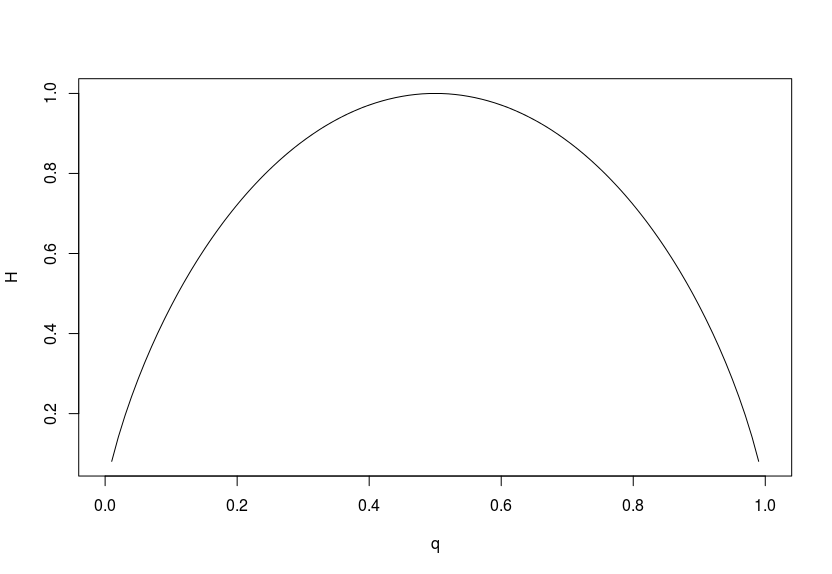
\includegraphics[scale=0.4]{entropy_function}
\caption{\label{fig:entropy_function}Binary Entropy Function}
\end{figure}

Next proposition shows that the maximum value for entropy is the logarithm of the number of symbols of $A$, and that this value is reached when all the symbols have the same probability.

\begin{proposition}
\label{prop:maximum_entropy}
Given the random variable $X$ we have that $H(X) \leq \log n$, and $H(X) = \log n$ if, and only if, $p(a_1) = p(a_2) = \ldots = p(a_n)$.
\end{proposition}
\begin{proof}
Consider the expression:
\[
\log n - H(X) = \sum_{i=1}^n p(a_i) \log n - \sum_{i=1}^n p(a_i) log {\frac{1}{p(a_i)}} = \sum_{i=1}^n p(a_i) \log n p(a_i)
\]
Applying property \ref{eq:change_base_logarithm} we have that:
\[
\log n - H(X) = \log e \sum_{i=1}^n p(a_i) \ln n p(a_i)
\]
And applying property \ref{eq:natural_logarithm_inequality} (equalling $x = 1 / n p(a_i)$):
\[
\log n - H(X) \geq \log e \sum_{i=1}^n p(a_i) \left( 1 - \frac{1}{n p(a_i)} \right) \geq \log e \left( \sum_{i=1}^n p(a_i) - \frac{1}{n} \sum_{i=1}^n \frac{p(a_i)}{p(a_i)} \right) \geq 0
\]
Which proves that $H(X) \leq \log n$.

The inequality becomes an equality if, and only if, $p(a_i) = 1 / n$ (given that the inequality \ref{eq:natural_logarithm_inequality} becomes an equality if, and only if, $x=1$).

\end{proof}

\begin{example}
If we choose a random symbol from $A$ according to the probability mass function $p$, entropy would be the minimum expected number of binary questions (Yes/No questions) required to identify the selected symbol. If the symbols of $A$ are equiprobable, the expected number of questions is maximal and equal to $\log d(A)$.
\end{example}

We can extend the concept of entropy to a pair of random variables by means of using the joint probability mass function. In this way, the joint entropy will be a measure of the uncertainty associated to both variables. Let $A = \{a_1, a_2, \ldots, a_n\}$ and $B = \{b_1, b_2, \dots, b_m\}$ two finite sets, and $X$ and $Y$ two random variables defined over the sets $A$ and $B$ respectively, with probability mass function $p(a)$ and $p(b)$, and joint probability mass function $p(a, b)$.

\begin{definition}
The \emph{joint entropy} of the random variables $A$ and $B$, denoted by $H(A, B)$, is defined as:
\[
H(A, B) = \sum_{a \in A} \sum_{b \in B} p(a, b) \log \frac{1}{p(a, b)}
\]
\end{definition}

Since $p(a, b) = p(b, a)$ we have that the joint entropy does not depend of the order in which the random variables are selected, that is $H(A, B) = H(B, A)$. We can provide a similar definition for the joint entropy of a set of $n$ random variables $A_1, A_2, \ldots, A_n$ using the joint probability mass function $p(a_1, a_2, \ldots, a_n)$.

Adding a second random variable whose outcome is not know might increase the entropy, as following proposition proves.

\begin{proposition}
We have that
\[
H(A, B) \geq \max \left( H(A), H(B) \right)
\]
\end{proposition}
\begin{proof}
\[
H(A, B) = \sum_{a \in A} \sum_{b \in B} p(a,b) \log \frac{1}{p(a,b)} \geq \sum_{a \in A} \sum_{b \in B} p(a,b) \log \frac{1}{p(a)} = \sum_{a \in A} p(a) \log \frac{1}{p(a)} = H(A)
\]
In the same way we can prove that $H(A, B) \geq H(B)$. Combining both inequalities we get the desired result.
\end{proof}

The joint entropy of two random variables cannot be greater that the sum of their individual entropies.

\begin{proposition}
\label{prop:joint_entropy}
We have that $H(A, B) \leq H(A) + H(B)$ and $H(A, B) = H(A) + H(B)$ if, and only if, $p(a)$ and $p(b)$ are statistically independent.
\end{proposition}
\begin{proof}
{\color{red} TODO: Prove without using the concept of conditional entropy nor mutual information.}
\end{proof}

% Conditional Entropy

The next derived concept from entropy that we are going to introduce is conditional entropy. Conditional entropy measures the uncertainty of a random variable given that the value of another random variable is known.

\begin{definition}
The \emph{conditional entropy} of the random variable $B$ given the random variable $A$, denoted by $H(B \mid A)$, is defined as:
\[
H(B \mid A) = \sum_{a \in A} \sum_{b \in B} p(a, b) \log \frac{1}{p(b \mid a)}
\]
\end{definition}

Since $p(b \mid a) \neq p(a \mid b)$ we have that $H(B \mid A) \neq H(A \mid B)$. If $H(B \mid A) = 0$ we have that the value of $B$ is completely determined by the value of $A$.

Next proposition proves that knowing the value of a second random variable can never increase the uncertainty of a random variable.

\begin{proposition}
Given the random variables $X$ and $Y$, we have that $H(Y \mid X) \leq H(Y)$, and $H(Y \mid X) = H(Y)$ if, and only if, $p(a)$ and $p(b)$ are independent.
\end{proposition}
\begin{proof}
\begin{multline}
H(Y \mid X) = \sum_{a \in A} \sum_{y \in B} p(a, b) \log \frac{1}{p(b \mid a)} = \sum_{a \in A} \sum_{b \in B} p(a, b) \log \frac{p(a)}{p(a, b)} \\
\notag = \sum_{a \in A} \sum_{b \in B} p(a, b) \log p(a) - \sum_{a \in A} \sum_{b \in B} p(a, b) \log p(a, b) = -H(X) + H(X, Y)
\end{multline}
Applying Propositon \ref{prop:joint_entropy} we have that $H(Y \mid X) = H(X, Y) - H(X) \leq H(X) + H(Y) - H(X) = H(Y)$.
The iff equality is also proved by applying Proposition \ref{prop:joint_entropy}.
\end{proof}

From an intuitive point of view we could expect that the uncertainty associated to a pair of random variables must be equal to the uncertainty of one of them plus the uncertainty of the second given that we know the outcome of the first one.

\begin{proposition}[Chain rule]
\label{prop:chain_rule_entropy}
Given the random variables $X$ and $Y$ we have that $H(X, Y) = H(X) + H(Y \mid X)$.
\end{proposition}
\begin{proof}
\begin{multline}
H(Y, X) = \sum_{a \in A} \sum_{b \in B} p(a, b) \log \frac{1}{p(a, b)} = \sum_{a \in A} \sum_{b \in B} p(a, b) \log \frac{1}{p(a) p(a \mid b)} \\
\notag = \sum_{a \in A} \sum_{b \in B} p(a, b) \log \frac{1}{p(a)} + \sum_{a \in A} \sum_{b \in B} p(a, b) \log \frac{1}{p(a \mid b)} = H(X) + H(Y \mid X)
\end{multline}
\end{proof}

% Mutual information

The last derived concept of entropy we are going to see is mutual information. Intuitively, the mutual information of two random variables $X$ and $Y$ measures the information that $X$ and $Y$ share, that is, how much knowing one of these variables reduces the uncertainty about the other.

\begin{definition}
The \emph{mutual information} of the random variable $X$ and $Y$, denoted by $I(X ; Y)$, is defined as:
\[
I(X ; Y) = \sum_{a \in A} \sum_{b \in B} p(a, b) \log \frac{p(a, b)}{p(a) p(b)}
\]
\end{definition}

Since $p(a, b) = p(b, a)$ we have that $I(X ; Y) = I(Y ; X)$, that is, the order of the random variables does not affect the concept of mutual information.

Next proposition shows that mutual information is a positive quantity, and it is equal to 0 if, and only if, the random variables are independent.

\begin{proposition}
Given the random variables $X$ and $Y$ we have that $I(X ; Y) \geq 0$, and $I(X ; Y) = 0$ if, and only if, the variables $X$ and $Y$ are independent.
\end{proposition}
\begin{proof}
{\color{red} TODO: to be done}
\end{proof}

{\color{red} Introduce this proposition}

\begin{proposition}
Given the random variables $X$ and $Y$, we have that:
\[
I(X;Y) = H(X) - H(X \mid Y) = H(Y) - H(Y \mid X)
\]
\end{proposition}
\begin{proof}
{\color{red} TODO: to be done}
\end{proof}

{\color{red} Introduce this proposition}

\begin{proposition}
Given the random variables $X$ and $Y$, we have that:
\[
I(X;Y) = H(X) + H(Y) - H(X, Y)
\]
\end{proposition}
\begin{proof}
{\color{red} TODO: to be done}
\end{proof}

{\color{red} Prove that $I(\mathcal{S}; \mathcal{S}) = H(\mathcal{S})$}

{\color{red} Use the Venn diagrams in this example}

\begin{example}
\end{example}

%
% Section: Huffman Algorithm
%

\section{Huffman Algorithm}
\label{sec:Huffman-Algorithm}

{\color{red} This section should be about compression algorithms. Not sure if only about algorithms based on information theory, or generic compression algorithms. Depends of what we need in practice}

{\color{red} Mention that Huffman is not necessarily the optimal compression algorithm}

From a practical point of view, there exists an algorithm, called \emph{Huffman algorithm}, that provides a method to build compact prefix-free codes given a probability distribution. For simplicity, we will study first the particular case of constructing binary prefix-free codes, and later I will provide its generalization to the case of D-ary prefix-free codes.

\begin{algorithm}
\caption{Huffman Algorithm}
\label{alg:Huffman}
\begin{algorithmic}
\Procedure{Huffman}{$Q$}
    \State $T \gets$ empty tree
    \For {$i \gets 1, d(Q) - 1$}
        \State allocate a new node $z$
        \State z.left = x = EXTRACT-MIN(Q)
        \State z.rigth = y = EXTRACT-MIN(Q)
        \State z.freq = x.freq + y.freq
        \State INSERT(Q, z)
    \EndFor
    \State \textbf{return} $T$
\EndProcedure
\end{algorithmic}
\end{algorithm}

The algorithm (see Algorithm \ref{alg:Huffman}) expects as input a source alphabet $\mathcal{S}=\left\{ s_{1},s_{2},\ldots,s_{q}\right\}$ and their corresponding probabilities $P = \left\{ p_{1}, p_{2}, \ldots, p_{q} \right\}$. For simplicity, we will merge both sets into a single one $Q = \left\{ (s_{1}, p_{1}), (s_{2}, p_{2}), \ldots, (s_{q}, p_{q}) \right\}$. The algorithm works by constructing a binary tree $T$, similar to the one used in the proof of Theorem \ref{th:Kraft-Inequality}. The algorithm requires $d(Q) - 1$ iterations to finish. During each iteration, the two elements with the lowest probability are selected and removed from set $Q$, and a new tree node $z$ is created, with the addition of the removed values, and added to the set $Q$. Once the tree has been constructed, we have to perform a tree transversal assigning a $0$ to each left branch, and a $1$ to each right branch, until we reach a leaf.

\begin{example}
Assume we have the source alphabet $\mathcal{S}=\left\{a, b, c, d, e, f\right\}$ with the associated probabilities $P = \left\{0.35, 0.16, 0.08, 0.12, 0.06, 0.23 \right\}$. In Figure \label{fig:Huffman-Algorithm} are depicted the contents of the set $Q$ and the tree $T$ for each iteration of the algorithm. At the end of the algorithm, if we perform a traversal of the $T$ tree, we will get the following prefix-free compact code for the source alphabet $S$: 

\bigskip

\centering
\begin{tabular}{l l}
\toprule
\textbf{Source Word} & \textbf{Code Word} \\
\midrule
a & 11   \\
b & 00   \\
c & 1011 \\
d & 100  \\
e & 1010 \\
f & 01   \\
\bottomrule
\end{tabular}

\bigskip

The expected length of the code is $L = 2.4$ , and its entropy is $\mathcal{H} \approx 2.34$. Since the set of probabilities is not D-adic ...

% Q: Shall I mention the expected length of a uniform code?

\end{example}

\begin{figure}[h]
\centering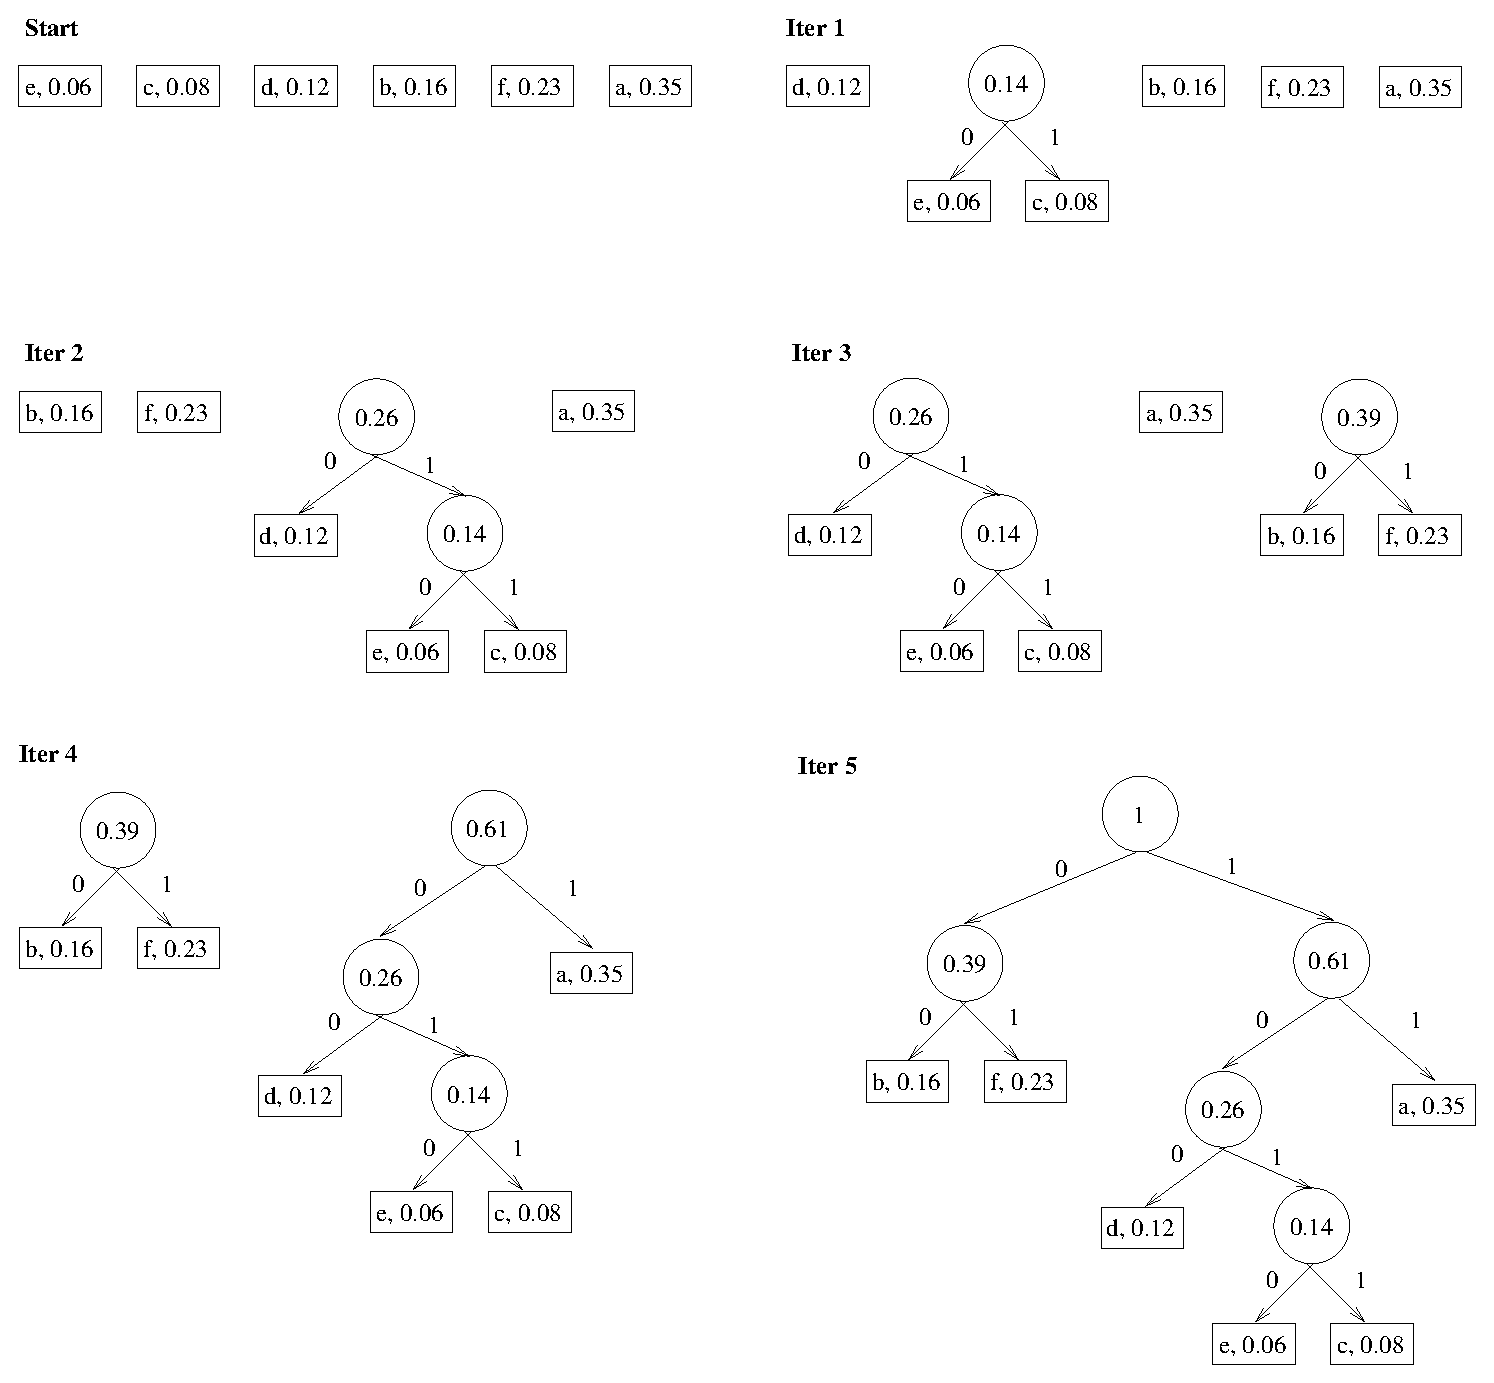
\includegraphics[scale=0.5]{huffman}
\caption{\label{fig:Huffman-Algorithm}Huffman Algorithm}
\end{figure}

\emph{This order is arbitrary; switching the left and rigth child of any node yields a different code of the same cost}

% Lemma would be better

\begin{proposition}
Given the probability is ...
\end{proposition}
\begin{proof}
{\color{red} TODO}
\end{proof}

The next theorem shows the optimality of the Huffman coding.

\begin{theorem}
If $C$ is a Huffman code then $C$ is compact.
\end{theorem}
\begin{proof}
{\color{red} TODO}
\end{proof}

{\color{red} TODO: Rewrite the following paragraphs}

\emph{So not only is this code optimal in the sense that no other feasible code performs better, but it is very close to the theoretical limit established by the entropy}

\emph{Although we have proved the theorem for a binary alphabet, the proof can be extended to establishing optimality of the Huffam coding algorithm for a D-ary alphabet as well.}

{\color{red} TODO: show how to extend the algorithm to D-ary codes}

\emph{Then -ary Huffman algorithm uses the {0, 1, ..., n-1} alphabet to encode message and build an n-ary tree [...] the same algorithm applies as for binary codes, except that the n least probable symbols are taken together , instead of just the 2 least probable. Note that for n greater than 2, not all sets of source words  can properly form an n-ary tree for Huffman coding. In this case, additional 0-probability place holders must be added. This is because the tree must form and n to 1 contractor; for binary coding, this is a 2 to 1 contractor, and any sized set can form such a contractor. If the number fo source words is congruent to 1 module n-1, then the set of source words will form a proper Huffman tree.}

{\color{red} Mention arithmetic coding}

%
% Section: Continuous Data
%

\section{Discretization Algorithms}
\label{sec:discretization_algorithms}

{\color{red} TODO: Rewrite this section.}

Let $\mathcal{X}$ a continuous random variable that follows a probability density function $P_\mathcal{X}$, and assume we have collected $n$ independent and identically distributed samples $\bold{x} = \{x_1, \ldots, x_n\}$ from $\mathcal{X}$. We are interested in computing the length of a compressed version of $\bold{x}$ using an optimal compressor. Unfortunately, and except for some degenerate distributions, there is no lossless compression algorithm that produces a string with fewer bits than encoding directly the elements $\bold{x}$. Compression algorithms for continuous data only work in case that the elements of $\bold{x}$ are not independent, as it is the case with images or sound. But, if this is not the case, the only option available to compress $\bold{x}$ is to use a lossy compression algorithm, where some information is lost.

We are looking for an algorithm to produce a finite non-overlapping partition of $m$ discrete intervals $D=\{ [d_o, d_1], (d_1, d_2], \ldots, (d_{m-1}, d_m] \}$, where $d_o = \min{\bold{x}_j}$, and $d_m = \max{\bold{x}_j}$, and $d_i < d_{i+1}$ for $i = 0, 1, \ldots, m-1$, assign a unique label to each interval, and encode the elements of $\bold{x}$ using this labeling schema. As compression algorithm we will use an optimal length code given the relative frequencies of the labels in the encoded vector. In this sense, our goal is to have a collection of intervals with sufficiently number of samples (so they are statistically significant) and that the distribution of frequencies resembles the original probability distribution $P_\mathcal{X}$.

A discretization algorithm is a mapping between a (possibly huge) number of numeric values and a reduced set of discrete values, and so, it is a process in which some information is potentially lost. The choice of discretization algorithm is something that could have a high impact in the practical computation of the nescience. We are interested in a discretization algorithm that produces a large number of intervals (low bias), with a large number of number of observations per interval (low variance). Common techniques include \emph{equal width discretization}, \emph{equal frequency discretization} and \emph{fixed frequency discretization}. However, these techniques require the optimization of an hyperparameter, and so, they are not suitable for our purposes.

In a \emph{proportional discretization approach} the number of intervals $m$ and the number of observations per interval $s$ are equally proportional to the number of observations $n$. The algorithm starts by sorting the values of $\bold{x}_j$ in ascending order and then discretizing them into $m$ intervals of approximately $s$ (possibly identical) values each. In this way, as the number of training observations increases, both interval frequency and number of intervals increases, taking advantage of the larger number of observations. In the same way, when the number of observations decreases, we reduce both.

\subsection{k-means Clustering}
\label{sec:kmeans_clustering}

K-means clustering is an algorithms that partitions n observations into k clusters in such a way that each observation belongs to the cluster with the nearest mean. In this way, we can replace the observation that belong to a cluster by its means, as a discretization. The optimization criteria in k-means is to minize the within-cluster variance. Given the fact that the problem is NP-Complete, some approximation algorithms are used instead.

{\color{red} TODO: Define the concept of Voronoi diagram / Voronoi cell}

\section*{References}

{\color{red} TODO: write this section}

In 1948, Claude E. Shannon published a paper entitled "A Mathematical Theory of Communication", where he established the foundations of a new discipline, later called \emph{information theory}.

Paper of Shannon ... Harley

Huffman -> D. A. Huffman. A method for the construction of minimum redundancy codes. Proc. IRE, 40:1098-1101, 1952.

The algorithm of huffman has been adapted from Cover. Here also you can find a proof that the algorithm is of order XX. 

Kraft's inequality was published by Leon G. Kraft in 1949 as part of his Master Thesis \cite{kraft1949device}. The inequality was independently rediscovered and proved for the general case of uniquely decodable codes by Brockway McMillan in 1956 \cite{mcmillan1956two}. The proofs contained in this book have been adapted from \cite{cover2012elements}.


The proof of proposition \ref{prop:maximum_entropy} has been adapted from \cite{abramson1963information}.
The proof of proposition 4.3.1 has been adapted from Abramson.

In the area of \emph{digital signal processing} \cite{gersho2012vector} it is common to apply a pre-processing step called \emph{quantization}, in which a large number of samples from a continuous signal are mapped into a finite number of representative values. It can be a \emph{scalar quantization} when the signal is one dimensional, or \emph{vector quantization} in case of a multidemensional signal. The optimization goal is to identify a (pre-defined) number of quantizied values such that the mean squared error between the selected values and the original signal is minimized. The problem is solved using the Lloyd-max algorithm \cite{lloyd1982least} (closely relted to the kmeans clustering algorithm \cite{} used in machine learning) in which the search space is paritioned in a collection of convex regions and their centroids used as quant, and then, are continously adapted until some stopping criteria is reached. Although it can be shown that the algorithm converges to the optimal solution that minimizes the mean squared error, the selected intervals cannot be used as estimation of the original probability distribution.






%
% CHAPTER: Algorithmic Information
%

%
% CHAPTER 4.- Kolmogorov Complexity
%

% TODO: Can we talk about independent topics? K(t|s) = K(t)
% TODO: Does K(t|s) != K(s|t)?


\chapterimage{Mandelbrot.pdf}

\chapter{Complexity}
\label{chap:Algorithmic_Information}

\begin{quote}
\begin{flushright}
\emph{Everything should be made as simple as possible, \\
but not simpler. \\}
Albert Einstein
\end{flushright}
\end{quote}
\bigskip

In Chapter \ref{chap:Coding}, the concept of the complexity of a string based on the lengths of the codewords of a prefix-free code was introduced. This definition is limited by two main factors: firstly, it necessitates prior knowledge of the set of possible strings, and secondly, it requires the definition of a probability distribution over this set a priori. It would be highly beneficial if we could expand the set of strings to encompass all strings (that is, $\mathcal{B}^\ast$) without necessitating a probability distribution, thereby providing an absolute notion of string complexity. Unfortunately, even if these issues are addressed, a more significant limitation exists in studying the complexity of strings using codes: certain strings, expected to be classified as simple, cannot be compressed. For instance, the binary expansion of the constant $\pi$ follows a uniform distribution over the set $\left\{0, 1\right\}$ and, as such, cannot be compressed. However, it can be fully and effectively described by a very short mathematical formula. This necessitates an alternative definition of string complexity.

\emph{Kolmogorov Complexity}, also known as \emph{Algorithmic Information Theory}, offers a definition of the complexity of a string that explicitly addresses these issues. Intuitively, the amount of information in a finite string is measured by the length of the shortest computer program capable of producing the string. This approach does not require prior knowledge of the set of valid strings or their probability distribution. Furthermore, objects like $\pi$ are appropriately classified as having low complexity. We could argue that Kolmogorov complexity provides a universal definition of the amount of information that closely aligns with our intuitive understanding. To compute the Kolmogorov complexity of a string, it is necessary to agree upon a universal description method or computer language, along with a universal computer. One might question whether, by doing so, the complexity of a string becomes dependent on the chosen computer language. Fortunately, it has been demonstrated that this is not the case, as all reasonable (and sufficiently powerful) computer languages yield the same description length, up to a fixed constant that depends on the languages chosen, but not on the string itself. Unfortunately, Kolmogorov complexity introduces a significant issue: it is a non-computable quantity, and as such, must be approximated in practice.

At this point, one might wonder if it is possible to compute the complexity of any object in general, not just strings. The answer is yes, at least theoretically. Given an object $x$, the task is to provide an encoding method that represents the object as a string  $x$. This encoding method would only be useful if we can losslessly and effectively reconstruct the original object from its encoded description. Unfortunately, providing such descriptions is not always feasible, either because the objects in question are abstract (as is often the case in mathematics) or because practical reconstruction of the object from its description is currently impossible (for example, with living organisms\footnote{As of now, it is not possible to recreate an animal solely based on its DNA.}).

%
% Section: String Complexity
%

\section{Strings Complexity}
\label{sec:strings_complexity}

In Section \ref{sec:Turing-Machines}, the concept of the Turing machine, an idealized model of computers, was introduced. We saw that Turing machines can be represented as partial computable functions $T:\mathcal{B}^\ast \rightarrow \mathcal{B}^\ast$, which assign to each input string $s \in \mathcal{B}^\ast$ an output string $T(s) \in \mathcal{B}^\ast$ (Definition \ref{def:computable-function}). We also introduced the concept of a universal Turing machine $U:\mathcal{B}^\ast \times \mathcal{B}^\ast \rightarrow \mathcal{B}^\ast$ (Definition \ref{def:Universal-Turing-Machine}), a machine that can simulate the behavior of any other Turing machine; that is, for all $(x,v) \in  \mathcal{B}^\ast \times \mathcal{B}^\ast$, we have that $U(x,v) = T_{x}(v)$. Later, in Section \ref{Codes}, the concept of a code, and in particular, the notion of a prefix-free code, was introduced (Definition \ref{def:Prefix-free-Code}). We saw that this kind of code presents important properties (Theorem \ref{th:Kraft-Inequality}). The next definition merges the best of both worlds, Turing machines and prefix-free codes, and introduces a new type of universal Turing machine.

\begin{definition}
A \emph{prefix-free universal Turing machine}\index{Prefix-free universal Turing machine} is a universal Turing machine $U:\mathcal{B}^\ast \times \mathcal{B}^\ast \rightarrow \mathcal{B}^\ast$ such that, for every $v \in \mathcal{B}^\ast$, the domain $U_{v}$ is prefix-free, where $U_{v}:\mathcal{B}^\ast \rightarrow \mathcal{B}^\ast$ and $U_{v}(p) = U(p, v)$ for all $p \in \mathcal{B}^\ast$.
\end{definition}

Using modern computer science terminology we could say that $U$ is the computer, $p$ is the program and $v$ is the input to the program. Intuitively, the above definition requires that no computer program can be a prefix of any other program. This is not a limitation from the point of view of string lengths, since, by applying McMillan's theorem (Theorem \ref{th:Kraft-Inequality}), given a uniquely decodable program, we could always find a prefix-free one that computes exactly the same function and has the same length. Moreover, in practice, real computer programs are usually prefix-free; for example, the C programming language requires that all functions must be enclosed by braces \{\}.

The concept of a prefix-free universal Turing machine allows us to introduce a new definition of the complexity of a string that aligns more closely with our intuitive understanding of the amount of computational information contained in an object (encoded as a string).

\begin{definition}[Kolmogorov Complexity]
\label{def:Kolmogorov-Complexity}\index{Kolmogorov Complexity}
Fix a prefix-free universal Turing machine $U:\mathcal{B}^\ast \times \mathcal{B}^\ast \rightarrow \mathcal{B}^\ast$. The \emph{Kolmogorov complexity} of a string $s \in \mathcal{B}^\ast$, denoted by $K(s)$, is defined as:
\[
K(s)=\min_{p,v \in \mathcal{B}^\ast}\left\{l(p) + l(v)\,:\, U(p,v)=s\right\}
\]
\end{definition}

Intuitively, the shortest description of a string $s$ is given by two elements: a program $p$ (a self delimited Turing machine) that compress all the regular patterns of the string, and a new string $v$ that comprises those parts of $s$ that do not present any regularity. We have to find the optimum balance between increasing the complexity of the program, trying to grasp more regularities, or increase the size of the non-compressible part\footnote{In the literature the Kolmogorov complexity of the string $s$ is defined as $K(s)=\min_{p \in \mathcal{B}^\ast}\left\{l(p)\,:\, U(p,\lambda)=s\right\}$, that is, the length of the shortest computer program that without any additional input can print the string $s$. We prefer to use the two parts definition $l(p) + l(v)$ because it is more in line with the requirements of the theory of nescience.}.

\begin{example}
Consider the string composed of one thousand times the substring "10", that is "$\underbrace{1010\ldots1010}_{1.000\,\mathrm{times}}$". We could write the following program:

\begin{verbatim}
    example(char *v) {
        for (int i=1; i<=1000; i++)
            printf("%s", v);
    }
\end{verbatim}
and then run it with:
\begin{verbatim}
    example("10");
\end{verbatim}

in order to print it. The length of the original string is 2.000 bits, but the length of the program is 480 bits (assuming that every symbol is encoded using an uniform code of 8 bits), and the length of the input is 2 bits, so we can conclude that the string has a low complexity. Of course, in order to compute the real Kolmogorov complexity of the string we should find the shortest Turing machine that prints that string.

On the contrary, a string composed of two thousands random 0's and 1's would have a high complexity, since it does not exists any program shorter than the program that prints the string itself.
\end{example}

As we mentioned in the preface of this chapter, Kolmogorov complexity would not be particularly useful if the complexity of strings depended on the choice of universal Turing machine. The following theorem demonstrates that this concern is unfounded, up to a constant that depends on the choice of machines, but not on the strings themselves. This establishes Kolmogorov complexity as an inherent property of the strings.

\begin{theorem}[Invariance theorem]
\label{def:Invariance-theorem}\index{Invariance Theorem}
Let $U$ and $U'$ two universal Turing machines. Then, there exists a constant $C_{U, U'}$, that depends on $U$ and $U'$, such that for each string $s \in \Sigma^{\ast}$ we have that:
\[
K_{U}(s) \leq K_{U'}(s) + C_{U, U'}
\]
\end{theorem}
\begin{proof}
Let $p, v$ be the shortest strings that $U'(p,v)=s$, then we have that $U(\langle U',p, v \rangle, \lambda) = U'(p, v) = s$, and that $l(\langle U',p \rangle) = \log(l(\langle U' \rangle)) + 1 + l(\langle U' \rangle) + l(p) = K_{U'}(s) + C$, where $l(\langle U' \rangle)$ is the length of the machine $U'$ using the encoding described in Section \ref{sec:Universal-Turing-Machines}.
\end{proof}

\begin{example}
Consider a universal programming language, such as Java, and an alternative language, such as Python. We can write a Python interpreter in Java, that is, a Java program that takes a Python script as input and executes it. Then, to compute the complexity of a string $s \in \mathcal{B}^\ast$ using Java, $C_J(s)$, it would be no greater than the complexity of the string using Python, $C_P(s)$, plus the length of the Python interpreter written in Java, $C_{J,P}$. Importantly, the length of the interpreter, $C_{J,P}$, does not depend on the string $s$.
\end{example}

Although we have proved that Kolmogorov complexity does not depend on the selected universal Turing machine, the size of the constant \(C_{U, U'}\) could pose a limitation in practical applications, especially when computing the complexity of short strings where the constant might significantly exceed the complexity of the string itself. This challenge is addressed by the Minimum Description Length principle, as described in Section \ref{sec:MML}.

\begin{notation}
We denote by \(s^\ast\) the shortest program that outputs the string \(s\) on the universal Turing machine \(U\), that is, \(s^\ast = \langle p,v \rangle\), \(U(s^\ast) = s\) and \(l(s^\ast) = K(s)\). If more than one program satisfies these properties, we select the first one using a lexicographical order induced by \(0 < 1\).
\end{notation}

The size of the \(C_{U, U'}\) constant is not the only challenge presented by Kolmogorov complexity; another issue is its non-computability, that is, there is no algorithm capable of determining the shortest program that generates any given string. The following theorem on the uncomputability of Kolmogorov complexity marks a pivotal insight into the intrinsic limits of complexity theory. By exploring the theorem, we delve into the heart of computability theory, confronting the paradoxical reality that some of the most fundamental aspects of information are inherently beyond the reach of algorithmic computation.

\begin{theorem}
The function \(K: \mathcal{B}^\ast \rightarrow \mathbb{N}\) that assigns to each string \(s\) its Kolmogorov complexity \(K(s)\) is not computable.
\end{theorem}
\begin{proof}
{\color{red} TODO: Review}
Assume for the sake of contradiction that \(K\) is computable. This means there exists a Turing machine \(T\) such that for any string \(s\), \(T\) halts with \(K(s)\) on its tape. Consider the following process, which uses \(T\) to construct a string \(s\) of arbitrary complexity: i) enumerate all binary strings using a shortlex ordering: \(s_1, s_2, \ldots\), ii) for each string \(s_i\), compute \(K(s_i)\) using \(T\) and select \(s_i\) such that \(K(s_i) > l(s_i) + C\), where \(C\) is a constant representing the length of this description plus the operation to add \(C\). Such a process would effectively produce a string \(s\) whose Kolmogorov complexity is greater than its length plus a constant, which contradicts the definition of Kolmogorov complexity as the length of the shortest description. The contradiction arises because our assumption that \(K\) is computable allows us to construct a string that defies the bounds set by \(K\) itself. Therefore, the function \(K\) is not computable.
\end{proof}

If \(K\) were computable, we could solve the Halting Problem by constructing a program that, for any input program and input, computes whether the program halts by checking if its Kolmogorov complexity is finite. Since the Halting Problem is known to be undecidable, this provides a contradiction.

In practice, we approximate the Kolmogorov complexity using the compressed version of the string, employing standard compression algorithms, such as the Huffman algorithm described in Section \ref{sec:Huffman-Algorithm}.

%
% Section: Properties of Kolmogorov Complexity
%

\section{Properties of Complexity}

In this section, we delve into the properties of Kolmogorov complexity. We will explore the foundational principles that govern this complexity measure, including its invariance, symmetry, and non-computability. Through examining these properties, we gain deeper insights into the complex interplay between information, computation, and randomness.

Kolmogorov complexity is a finite positive natural number.

\begin{proposition}
For all $s\in\mathcal{B}^{\ast}$ we have that $0 < K(s) < \infty$.
\end{proposition}
\begin{proof}
Since $K(s)$ is the length of a string, it must be greater than $0$. The property $K(s) < \infty$ is a consequence of Proposition \ref{prop:kolmogorov_length} and the fact that we are only dealing with finite strings.
\end{proof}

The Kolmogorov complexity of a string cannot surpass the sum of its own length and a constant.

\begin{proposition}
\label{prop:kolmogorov_length}
There is a constant $c$ such that for all $s\in\mathcal{B}^{\ast}$ we have that $K(s) \leq l(s) + c$.
\end{proposition}
\begin{proof}
Let $s \in \mathcal{B}^\ast$ be an arbitrary string, and consider the encoding of a Turing machine $p$ such that for any input $v = s$, it halts and outputs $s$. The program $p$ is designed to simply reproduce its input. Given this setup, when $p$ is executed on a universal Turing machine $U$ with $s$ as input, it satisfies the condition $U(p, s) = s$. The length of \(p\) is a constant $c$ across all strings $s$. This constancy arises because $p$'s mechanism (accepting an input and outputting it unchanged) does not vary with the size or content of $s$. By the definition of Kolmogorov Complexity $K(s)$, which seeks the minimum length of a program-input pair that generates $s$, the combination of $p$ and $s$ presents a feasible solution. Therefore, we have $K(s) \leq l(s) + l(p) = l(s) + c$.
\end{proof}

The size of the constant $c$ depends on the specific encoding schema used by the selected universal Turing machine $U$, but it is independent of the string $s$. In Section \ref{sec:incompressibility_randomness}, we will explore the characteristics of random strings, which are defined as strings that cannot be compressed. Such strings exhibit a Kolmogorov complexity that exceeds their own length, that is, $K(s) > l(s)$.

The absolute difference in Kolmogorov complexity between any string \(x\) and its transformed counterpart \(f(x)\), via a computable bijection, is bounded by a constant $c$. That is, not only does $f$ not increase the complexity of $x$ by more than a constant, but also $f$ does not decrease the complexity by more than a constant.

\begin{proposition}
Let $f:\mathcal{B}^{\ast} \to \mathcal{B}^{\ast}$ is a computable biyection, then there exists a constant $c$ such that $| K\left( f(x) \right) -  K(x) | < c$.
\end{proposition}
\begin{proof}
Let $P_f$ be the program that computes $f$ and $P_{f^{-1}}$ the program that computes the inverse of $f$. For any string $x$, let $P_x$ be the shortest program that generates $x$. Then, a program $P_{f(x)}$ that generates $f(x)$ can be constructed by concatenating $P_x$ with $P_f$. The length of this program is $|P_{f(x)}| = |P_f| + |P_x|$. Since $|P_f|$ is a constant that does not dependent on $x$, we can say that $K(f(x)) \leq K(x) + |P_f|$. Similarly, given $f(x)$, we can construct a program $P'_{x}$ to generate $x$ by applying $P_{f^{-1}}$ to $f(x)$. The length of this program is $|P'_{x}| = |P_f| + |P_{f^{-1}}|$. Thus, $K(x) \leq K(f(x)) + |P_{f^{-1}}|$. The two inequalities combined implies that $|K(f(x)) - K(x)| \leq \max(|P_f|, |P_{f^{-1}}|) = c$, where \(c\) is a constant that represents the maximum of the lengths of the programs that compute \(f\) and \(f^{-1}\). This constant \(c\) does not depend on \(x\), but rather on the complexity of the functions \(f\) and \(f^{-1}\).
\end{proof}

This proposition shows a remarkable stability of informational content under computable bijections, underscoring the intrinsic robustness of Kolmogorov complexity in the face of such transformations.

\begin{example}
{\color{red} TODO: Provide an example clarifying this concept.}
\end{example}

%
% Section: Joint Kolmogorov Complexity
%

\section{Joint Kolmogorov Complexity}

The joint Kolmogorov complexity of two strings $s$ and $t$ is defined as the length of the shortest is the shortest program $p$ that, when executed on an universal Turing machine $U$, outputs the pair $\langle s, t \rangle$, that is, in such a way that allows both strings to be unambiguously retrieved.

\begin{definition}[Joint Kolmogorov Complexity]
\label{def:Joint-Kolmogorov-Complexity}\index{Joint Kolmogorov complexity}
The \emph{Joint Kolmogorov complexity} of the strings $s, t \in \mathcal{B}^\ast$, denoted by $K(s, t)$, is defined as:
\[
K(s, t)=\min_{p,v \in \mathcal{B}^\ast}\left\{l(p) + l(v)\,:\, U(p,v)=\langle s, t \rangle \right\}
\]
\end{definition}

The notation $K(s, t)$ and $K(st)$ represent two different concepts in the context of Kolmogorov complexity. $K(s, t)$ refers to the joint Kolmogorov complexity of two strings $s$ and $t$ as per Definition \ref{def:Joint-Kolmogorov-Complexity}, meanwhile $K(st)$ represents the Kolmogorov complexity of the concatenation of $s$ and $t$, without any additional structure to distinguish between them, and so, Defintion \ref{def:Kolmogorov-Complexity} is applied. The choice between $K(s, t)$ and $K(st)$ depends on whether it's important to preserve and utilize the distinction and relationship between $s$ and $t$. If analyzing the interplay or the shared characteristics of $s$ and $t$ is relevant, $K(s, t)$ is more appropriate. If the focus is on the information content of the combined sequence without regard to its origin from two separate strings, $K(st)$ is used.

\begin{example}
{\color{red} TODO: Provide an example clarifying this concept.}
\end{example}

Our first proposition highlights a fundamental symmetry in Kolmogorov complexity, illustrating that the complexity of describing a pair of strings in either order differs by at most a constant. This reflects the intrinsic property that the information content is independent of the specific arrangement of the strings being described. The constant \(c\) encapsulates the overhead associated with the operations needed to reverse the order of the strings.

\begin{proposition}
\label{prop:kolmogorov_order}
There is a constant $c$ such that for all $x, y \in\mathcal{B}^{\ast}$ we have that $K(x, y) \leq K(y, x) + c$.
\end{proposition}
\begin{proof}
The key to this proof lies in the symmetry of information and the properties of a universal Turing machine. Let $U$ be a universal Turing machine, and let $p_{xy}$ and $p_{yx}$ be the shortest programs that output $x$ followed by $y$, and $y$ followed by $x$, respectively, when executed on $U$. To convert $p_{xy}$ into a program that outputs $yx$, we need to add or modify a finite set of instructions to swap the output order. This set of instructions has a fixed length, denoted by $c$. Therefore, the program that first computes $x$ and $y$ and then swaps their order can be at most $c$ bits longer than the program that directly computes $y$ and $x$.
\end{proof}

Next proposition underscores the subadditive nature of Kolmogorov complexity, proving that the total complexity of describing two strings jointly cannot exceed the sum of their individual complexities by more than a fixed constant, irrespective of the strings' content.

\begin{proposition}
\label{prop:additive_kolmogorov}
There is a constant $c$ such that for all $s, t \in\mathcal{B}^{\ast}$ we have that $K(s, t) \leq K(s) + K(t) + c$.
\end{proposition}
\begin{proof}
Let $s^\ast$ and $t^\ast$ be the shortest computer programs that generate $s$ and $t$, respectively. Given that $s^\ast$ and $t^\ast$ are designed to be prefix-free, a universal Turing machine $U$ can unambiguously decode each program without needing any additional information and subsequently generate the strings $s$ and $t$. The constant $c$ accounts for the requirement of $U$ to prepend the concatenated program for $st$ with the length $l(s)$ of $s$. This step ensures that the concatenated sequence $st$ can be decoded unambiguously.
\end{proof}

The last proposition states the relationship between the complexity of individual strings and their joint complexity, by establishing a lower bound on the joint complexity of two strings relative to their individual complexities.

\begin{proposition}
\label{prop:excess_kolmogorov}
There is a constant $c$ such that for all $s, t \in \mathcal{B}^{\ast}$ we have that $K(s, t) \geq K(s) + c$ and $K(s, t) \geq K(t) + c$.
\end{proposition}
\begin{proof}
Assume for the sake of contradiction that $K(s, t) < K(s) + c$. Let $p$ be the shortest computer program that outputs the pair $\langle s, t \rangle$, meaning that $K(s, t) = l(p)$. Since program $p$ unambiguously generates $s$ as part of the output pair, it follows that the complexity of generating $s$ alone, $K(s)$, should not exceed the length of $p$. which is a contradiction with respect the intial assumption of $K(s, t) < K(s) + c$. 
\end{proof}


%
% Section: Conditional Kolmogorov Complexity
%

\section{Conditional Kolmogorov complexity}

In this section, we explore the concept of \emph{conditional Kolmogorov complexity}, which examines how the complexity of a string $s$ can be significantly decreased by assuming prior knowledge of another string $t$. This notion highlights the impact of assuming some background information on the compressibility of a description.

\begin{definition}[Conditional Kolmogorov Complexity]
\index{Conditional Kolmogorov complexity}
The \emph{conditional Kolmogorov complexity} of a string $s \in \mathcal{B}^{\ast}$ given the string $t \in \mathcal{B}^{\ast}$ is defined as:
\[
K(s|t)=\min_{p, v \in \mathcal{B}^{\ast}}\left\{l(p) + l(v)\,:\, U(p,\langle v, t \rangle)=s\right\}
\]
\end{definition}

Similar to the non-conditional Kolmogorov complexity, the conditional complexity of a string $s$, given a background string $t$, depends on the strings themselves rather than the specific universal Turing machine used for computation. That is, for any two universal Turing machines, $U$ and $U'$, it is easy to show that there exists of a constant $C_{U, U'}$ such that for all strings $s, t \in \Sigma^{\ast}$, the inequality $K_{U}(s|t) \leq K_{U'}(s|t) + C_{U, U'}$ holds. This property underscores the inherent machine-independence of conditional complexity measures.

\begin{example}
{\color{red} TODO: Provide an example clarifying this concept.}
\end{example}

As it was the case of the unconditional Kolmogorov complexity, conditional Kolmogorov complexity is a finite positive natural numbrer.

\begin{proposition}
For all $s, t \in\mathcal{B}^{\ast}$ we have that $0 < K(s | t) < \infty$.
\end{proposition}
\begin{proof}
Since $K(s)$ is the length of a string, it must be greater than $0$. The property $K(s | t) < \infty$ is a consequence of Proposition \ref{prop:kolmogorov_length} and the fact that we are only dealing with finite strings.
\end{proof}

Next proposition posits that when a string $s$ is conditioned upon itself, its complexity stabilizes to a universal constant $c$.

\begin{proposition}
\label{prop:self_conditional}
There is a constant $c$ such that for all $s\in\mathcal{B}^{\ast}$ we have that $K(s | s ) = c$.
\end{proposition}
\begin{proof}
When a string $s$ is conditioned on itself, the information needed to generate $s$ from $s$ can be encapsulated in a Turing machine that simply copies its input to its output. This machine, being independent of the specific content of $s$, has a fixed length $c$. 
\end{proof}

This proposition explores the relationship between unconditional and conditional Kolmogorov complexities, establishing an upper bound for the latter. It asserts that for any strings $s$ and $t$, the complexity of $s$ given $t$ is at most the complexity of $s$ alone, plus a constant $c$. This highlights the intuitive notion that having additional information at most reduces the complexity of describing a string, or in the worst case, adds a constant overhead, but does not increase it beyond this bound.

\begin{proposition}
\label{prop:kolmogorov_conditional}
There is a constant $c$ such that for all $s, t \in \mathcal{B}^{\ast}$ we have that $K(s | t ) \leq K(s) + c$.
\end{proposition}
\begin{proof}
There exists a Turing machine $T'$ that ignores its input and $t$ directly generates $s$. The length of $T'$ is $K(s)$ by definition.
\end{proof}

The relationship between conditional, unconditional, and joint Kolmogorov complexities, offers a comprehensive perspective on the informational interdependencies of binary strings. It posits that the complexity of a string $s$ given another string $t$ is at most the complexity of $s$ alone, which in turn is no greater than the joint complexity of both $s$ and $t$. The proposition encapsulates the intuitive understanding that knowledge of additional data (in this case, $t$) cannot increase the complexity of describing $s$, and that the combined description of two strings is at least as complex as describing each independently.

\begin{proposition}
\label{prop:kolmogorov_relations}
For all $s, t\in\mathcal{B}^{\ast}$ we have that $K(s | t ) \leq K(s) \leq K(s, t)$.
\end{proposition}
\begin{proof}
Given Proposition \ref{prop:kolmogorov_conditional} and Proposition \ref{prop:excess_kolmogorov}.
\end{proof}

The Kolmogorov complexity chain rule is a fundamental principle that connects the joint complexity of two strings with their individual and conditional complexities. It asserts that the total complexity of a pair of strings $s$ and $t$ can be decomposed into the complexity of $s$ plus the complexity of $t$ given $s$. This relationship mirrors the additive property of entropy in information theory ({\color{red} see Proposition XXX}) and provides a powerful tool for understanding the interplay between information content and conditional information in the context of Kolmogorov complexity.

\begin{proposition}
\label{prop:kolmogorov_chain_rule}
For all $s, t \in \mathcal{B}^{\ast}$ we have that $K(s, t) = K(s) + K(t \mid s)$
\end{proposition}
\begin{proof}
{\color{red} TODO}
\end{proof}

\begin{example}
{\color{red} TODO: Provide an example clarifying this concept.}
\end{example}

%
% Section: Information Distance
%

\section{Information Distance}
\label{sec:information_distance}

In this section, we aim to introduce a universal metric for quantifying the absolute information distance between two or more individual entities encoded as strings of symbols. Intuitively, the information distance between two strings $s$ and $t$ can be understood as the length of the shortest computer program for a universal computer that enables the generation of $s$ given $t$ and vice versa.

\begin{definition}
The \emph{information distance}\index{Information distance} between two strings $s,  t \in \mathcal{B}^{\ast}$ with respect to a universal Turing machine $U$, denoted by $ID_U(s, t)$, is defined as
\[
ID_U(s, t) = \min \{ l(p) : U(p, s) = t, U(p, t) = s \}
\]
\end{definition}

It can be shown that for any pair of universal Turing machines, $U_1$ and $U_2$, the information distance between two strings $s$ and $t$ differs by no more than a constant $c$; this constant $c$ depends on the choice of $U_1$ and $U_2$ but is independent of the specific strings $s$ and $t$. It's also important to note that despite its theoretical utility, information distance is non-computable, meaning it does not exists and algorithm to calculate it in practice.

The idea of using the conditional Kolmogorov complexity of $s$ given $t$,that is $K(s \mid t)$, as a metric for information distance may seem appealing. However, this approach is unsuitable for capturing the essence of information distance because of its inherent asymmetry (refer to Proposition {\color{red} XXX}). For example, the complexity $K(\lambda \mid t)$ remains minimal even when $t$ significantly differs from the empty string. Alternatively, employing the sum $K(s \mid t) + K(t \mid s)$ as a measure of distance is also inadequate, as it overlooks the redundancy in the information necessary for transforming $s$ into $t$ and vice versa.

Next proposition shows the proper way in which the information distance between two strings can be computed using their conditional Kolmogorov complexity.

\begin{proposition}
Let $s,  t \in \mathcal{B}^{\ast}$ be two binary strings, then we have that:
\[
ID_U(s, t) = \max\{ K(s \mid t), K(t \mid s) \} + O ( \log \max\{ K(s \mid t), K(t \mid s) \}) 
\]
\end{proposition}
\begin{proof}
{\color{red} TODO: based on the maximal overlap.}
\end{proof}

\begin{example}
{\color{red} TODO: Give an example based on the bitwise exclusive or.}
\end{example}

{\color{red} Introduce the concept of max distance as:}
\[
E(x, y) = \max\{ K(x \mid y), K(y \mid x) \}
\]

{\color{red} Introduce the following proposition.}

\begin{proposition}
{\color{red} $E(x, y)$ is a metric.}
\end{proposition}
\begin{proof}
\end{proof}

{\color{red} Introduce the following proposition.}

\begin{proposition}
\[
E(x, y) = \max\{ K(x \mid y), K(y \mid x) \} = K(xy) - \min\{ K(x), K(y) \} + O(\log K(xy) )
\]
\end{proposition}
\begin{proof}
{\color{red} TODO: Pending}
\end{proof}

{\color{red} TODO: Introduce the concept of admisible information distance. Prove that $E(x, y)$ is an admisible information distance. Prove that it is minimal for every admisible information distance. Explain this notion of universality.}

{\color{red} This concept of information distance is universal because it encompasses all other computable distance metrics as special cases.}

\subsection*{Normalized Information Distance}

Information distance is an absolute measure; however, when assessing similarity, we are often more concerned with relative measures. For instance, consider two strings each of length 1,000,000 that differ by 1000 bits; we would perceive these strings as being relatively more similar compared to two strings of length 1000 bits that differ by the same amount of 1000 bits. This concept of normalization implies that the size of the description required for transformation should be evaluated in the context of the sizes of the objects involved.

\begin{definition}
The \emph{normalized information distance}\index{Normalized information distance} between two binary strings $s,  t \in \mathcal{B}^{\ast}$, denoted by $e(s, yt)$, is defined as:
\[
NID(s, t) = \frac{\max\{ K(s \mid t), K(t \mid s) \}}{\max \{ K(s), K(t) \} }
\]
\end{definition}

As expected, the normalized information distance is a number between zero and one.

\begin{proposition}
\label{prop:ncd_between_zero_and_one}
The normalized information distance $NID(s, t)$ takes values in the range $[0, 1]$.
\end{proposition}
\begin{proof}
{\color{red} TODO: Pending}
\end{proof}

{\color{red} Introduce the following proposition.}

\begin{proposition}
The normalized information distance $NID(x, y)$ is a metric, up to negligible errors.
\end{proposition}
\begin{proof}
{\color{red} TODO: Pending}
\end{proof}

{\color{red} Introduce the following proposition.}

\begin{proposition}
\[
NID(x, y) = \frac{ K(xy) - \min\{ K(x), K(y) \} + O(\log K(xy) ) }{ \max \{ K(s), K(t) \} }
\]
\end{proposition}
\begin{proof}
{\color{red} TODO: Pending}
\end{proof}

\subsection*{Normalized Compression Distance}

Although the normalized information distance metric is not computable, it has a potential wide range of applications. By approximating $K$ with practical compressors, where $Z(s)$ represents the binary length of the string $s$ compressed using a compressor $Z$ (such as "gzip", "bzip2", "PPMZ"), we can approximate the concept of normalized information distance. 

\begin{definition}
The \emph{normalized compression distance}\index{Normalized compression distance} between two strings $s,  t \in \mathcal{B}^{\ast}$, given the compressor $Z$, and denoted by $NCD_Z(s, t)$, is defined as:
\[
NCD_Z(s, t) = \frac{\max\{ Z(s \mid t), Z(t \mid s) \}}{\max \{ Z(s), Z(t) \} }
\]
\end{definition}

Unfortunately, for the majority of the compressors it is very difficult to compute the compressed conditional version of a string $Z(s \mid t)$. Fortunately, we can rewrite the NCD in a differnt way in which we do not need to use conditional compressions.

\begin{proposition}
The normalized compression distance between two strings $s,  t \in \mathcal{B}^{\ast}$, given the compressor $Z$, satisfies:
\[
NCD_Z(s, t) = \frac{ Z(st) - \min\{ Z(s), Z(t) \}}{\max \{ Z(s), Z(t) \} }
\]
\end{proposition}
\begin{proof}
{\color{red} TODO: prove.}
\end{proof}

The normalized compression distance constitutes a spectrum of distances, each defined by the choice of compressor $Z$. The effectiveness of $Z$ determines how closely the normalized compression distance mirrors the normalized information distance, ultimately influencing the quality of the outcomes.


%
% Section: Incompressibility and Randomness
%

\section{Incompressibility and Randomness}
\label{sec:incompressibility_randomness}

A string is considered incompressible if its Kolmogorov complexity is approximately equal to its length; in other words, there is no significantly shorter description or program that can produce it.

\begin{definition}
For each constant $c$ we say that a string $s \in \mathcal{B}^{\ast}$ is \emph{c-incompressible}\index{Incompressible string} if $K(s) \geq l(s) - c$.
\end{definition}

Next proposition shows that there exists incompressible strings for all strings lenghts.

\begin{proposition}
For every length $n$, there exists a string of length $n$ that is incompressible.
\end{proposition}
\begin{proof}
By a counting argument, the number of possible programs of length less than $n$ is less than $2^n$, which is the number of binary strings of length $n$. Therefore, some strings of length $n$ cannot be generated by any shorter program, rendering them incompressible.
\end{proof}

We will extend the term \emph{incompressible string} to encompass all the strings that are $c$-incompressible with small $c$. In this sense, it turns out that most strings are incompressible.

\begin{proposition}
For any $n$, at least $1 - \frac{1}{c}$ fraction of the strings of length $n$ are $c$-incompressible.
\end{proposition}
\begin{proof}
Consider the number of programs of length $n - c$ or less. There are $\sum_{i=0}^{n-c} 2^i = 2^{n-c+1} - 1$ such programs. Since there are $2^n$ strings of length $n$, and fewer than $2^{n-c+1}$ programs to generate them, at least $2^n - 2^{n-c+1} + 1$ strings of length $n$ must be $c$-incompressible. The fraction of incompressible strings is therefore at least $1 - \frac{2^{n-c+1} - 1}{2^n}$, which approximates $1 - \frac{1}{c}$ for large $n$.
\end{proof}

The notion of randomness, especially in the context of sequences or strings, is often intuitively associated with unpredictability, lack of pattern, or absence of structure. Kolmogorov complexity formalizes this intuition by linking randomness to incompressibility. Specifically, a string is considered to exhibit randomness if it cannot be generated by any program significantly shorter than the string itself.

\begin{definition}
We say that a string $s \in \mathcal{B}^{\ast}$ is \emph{random}\index{Random string} if it is $c$-incompressible with $c$ being small.
\end{definition}

Random strings are characterized by high Kolmogorov complexity, which means they are incompressible. Such strings contain the maximum amount of information possible, precluding the possibility of a simpler, algorithmic shorthand for their representation. This is because the shortest program that can generate a random string is essentially the string itself.

\begin{example}
Consider a string generated by flipping a fair coin to decide each bit: $1011010110110101$. Assuming the coin flips are truly random, this string's Kolmogorov complexity is high, as there's no shorter program or pattern that can generate it besides enumerating the bits one by one. Any attempt to compress it would result in a program whose length is comparable to the string itself.
\end{example}

The unpredictability of random strings stems from their incompressibility. Since predicting any subsequent bit of a random string essentially requires knowledge of the entire string (due to the lack of patterns), such strings are inherently unpredictable.

Random strings are typical in the space of all strings. Most strings are random in the sense of Kolmogorov complexity, implying that most strings do not admit a significantly shorter description. This aligns with the principle that, in a large enough set of strings, structured or simple patterns are the exception rather than the rule.

\begin{example}
Consider the set of all conceivable high-resolution digital photographs, each represented as a binary string encoding pixel colors and intensities. Within this immense collection, only a small fraction might display identifiabe patterns or motifs, such as a picture of a blue sky or a uniform monochromatic background. These images could be succinctly described or compressed into shorter binary sequences because their repetitive nature or constrained color palettes. However, the vast majority of these possible digital photographs bear resemblance to "random" strings, in the sense that they exhibit incompressible patterns.
\end{example}

%
% Section: Bibliography and References
%

\section*{Bibliography and References}

{\color{red} TODO: Section Pending!}

{\color{red} Kolmogorov Complexity, a fundamental concept in the field of information theory and computer science, emerged in the 1960s from the work of three pioneering researchers: Andrei Kolmogorov, Ray Solomonoff, and Gregory Chaitin. Independently arriving at similar concepts, these scholars sought to formalize a measure of the information content or complexity of an object (specifically, finite strings) in a way that is independent of the specific language or encoding used. Kolmogorov, a prominent Soviet mathematician, introduced his formulation in 1965, aiming to provide a theoretical foundation for understanding the complexity of individual objects beyond the probabilistic framework of Shannon's information theory. Solomonoff, an American information theorist, introduced a related concept as part of his work on algorithmic probability, emphasizing its implications for prediction and inductive inference. Chaitin, working in the United States as well, contributed by exploring the mathematical properties and implications of this notion, including its non-computability. The motivations behind the development of Kolmogorov Complexity were multifaceted, encompassing the desire to better understand the nature of information, randomness, and the limits of computation and prediction, thus laying the groundwork for numerous applications in theoretical computer science, mathematics, and beyond. }


The idea of measuring the amount of information contained in a string based on the shorter computer program that can reproduce it was introduced independelntly by Solomonoff \cite{solomonoff1964formal}, Kolmogorov \cite{kolmogorov1965three} and Chaiting \cite{chaitin1969simplicity}.

In the Kolomogorov complexity literature, the concept of Kolmogorov complexity is defined in terms of computable functions, i.e. Turing machines. Then it is shown that there are some machines that do not provide worse descriptiosn than others, up to a constant. And finally, it is proved that unversal Turing machines are not worse than any other machines. We have provided here an easier to understand short-cut to this approach. Also, we do not consider the case of of non-prefix Kolmogorov complexity. And we prefer to split code and data. See XX, XX, XX, or XX for a more classical introduction to Kolmogorov complexity.



%
% CHAPTER: Learning
%

%
% CHAPTER 5.- The MDL Principle
%

\chapterimage{TuringMachine.pdf} % Chapter heading image

\chapter{Learning}
\label{ch:Learning}

\begin{quote}
    \begin{flushright}
        \emph{All great work is the fruit of patience and perseverance,\\
            combined with tenacious concentration on a subject\\
            over a period of months or years.}\\
        Santiago Ramón y Cajal
    \end{flushright}
\end{quote}
\bigskip

{\color{red} Warning: This section still requires a significant amount of work!}

Machine learning refers to a large collection of algorithms designed to automatically build mathematical models based on sample data sets, usually with the aim of making predictions, classifying objects, or simply to better understand the structure of the data. In the past decade, machine learning algorithms have been highly successful in areas like self-driving cars, practical speech recognition, effective web search, and purchase recommendations.

In this chapter we are going to see how the problem of learning from data is formally formulated in the area of machine learning. In this sense, the chapter is a continuation of the introduction to discrete probability included in Section \ref{sec:discrete_probability}. Also, we are going to study in detail two particular approaches to machine learning that are highly related to our theory of nescience: the Minimum Description Length principle and the Minimum Message Length principle.

Most of the learning algorithms used today in practice are known since forty years ago. The high success of current machine learning applications is largely due to the availability of huge, high-quality, training datasets, and to the advance of computing power, and in particular, thanks to the powerful graphical processing units (GPU) used in video-games. In Chapter \ref{chap:Machine-Learning} we will introduce a collection of new machine learning algorithms based on the theory of nescience, and we will compare them with the current, state of the art, algorithms.

%
% Statistical Inference
%

\section{Statistical Inference}

\emph{Statistical inference} is the branch of probability and statistics concerned with deducing the probabilistic model behind a population after analyzing some data that, we believe, contain relevant information. Statistical inference is different from the area of \emph{descriptive statistics}, where the goal is to provide a summary of the main properties of the observed data, and \emph{probability theory}, that deals with the theoretical foundations. From the area of statistical inference, we are mostly interested in \emph{model selection} and \emph{point estimation}. Other techniques, like \emph{confidence intervals}, \emph{hypothesis testing} or \emph{experiment design} are not covered in this short review since they are not needed in the book.

\begin{definition}
    A \emph{statistical model} is a random variable, together with a specification of its probability distribution, and the identification of the parameters, denoted by $\theta$, of that distribution. When the parameter $\theta$ is unknown, it is said that the distribution of the random variable is conditional to $\theta$.
\end{definition}

We assume that the actual value of the unknown parameter $\theta$ can be inferred, usually trough a collection of data samples. The parameter $\theta$ could be a single scalar or a vector of values, and it is considered a random distribution as well. The set $\Theta = \{ \theta_1, \theta_2, \ldots \}$ composed by all the possible values of the parameter $\theta$ is called the \emph{parameter space}.

\begin{example}
\label{ex:binomial}
The binomial distribution with parameters $n$ and $p$ is a model for a family of experiments in which we are interested to know the number of successes in a sequence of $n$ independent binary trials (that is, each trial could be either a success or a failure), being the probability of success $p$. If $X$ is a random variable following a binomial distribution, denoted by $X \sim B(n,p)$, the probability of getting exactly $k$ successes is given by:
\[
    Pr(X=k) = {\binom {n}{k}}p^{k}(1-p)^{n-k}
\]
In statistical inference we are usually interested in the inverse problem. That is, we have the actual result of an experiment composed by $n$ samples, in which we know how many success $k$ we have got, and we would like to know the probability $p$ of success.
\end {example}

\begin{definition}
    A \emph{statistical inference} is a probabilistic statement about one of the elements of a statistical model.
\end{definition}

On the contrary of what happens with logical deduction, where we can be sure about the trueness of a conclusion, in case of induction and inference, the knowledge gathered is not conclusive. Probability theory is the tool we use to deal with the uncertainty of statistical inferences.

\begin{definition}
    Let $X_1, \ldots, X_n$ be $n$ random variables. A \emph{statistic} is a random variable $T = r \left( X_1, \ldots, X_n \right)$, where $r()$ an arbitrary real-valued function of $n$ variables.
\end{definition}

The mean and the standard deviation are examples of statistics.

    {\color{red} TODO: Explain why it is important the concept of "statistic", including an example.}

\begin{definition}
    Let $f$ be the distribution of a random variable $X$ with parameter $\theta$. We call $Pr(\theta)$ the \emph{prior distribution} of the parameter $\theta$.
\end{definition}

$Pr(\theta)$ is called the prior distribution because it is the distribution of the parameter $\theta$ that we have before observing any samples of data. The prior distribution is also the marginal distribution of $f(x \mid \theta)$ for all the possible samples $x$.

\begin{definition}
    Let $f$ be the distribution of a random variable $X$ with parameter $\theta$. We call $Pr(\theta \mid X)$ the \emph{posterior distribution} of the parameter $\theta$.
\end{definition}

... conditionoal distribution of the parameter $\theta$ given the observed data $x$ ...

% Non-Bayesian Inference

\subsection{Non-Bayesian Inference}

We would like to infer a statement about which model, or which parameters for a model, we should prefer given the collected data.

\begin{definition}
    Let $f$ be the distribution of a random variable $X$ with parameter $\theta$. We call $Pr(X \mid \theta)$ the \emph{likelihood function}.
\end{definition}

{\color{red} Maximum likelihood estimation is a method that determines values for the parameters of a model. The parameter values are found such that they maximise the likelihood that the process described by the model produced the data that were actually observed.}

Let $\Theta$ be a family of models (probability distributions) with a discrete parameter $\left\{ \theta_1,\theta_2,\ldots \right\}$ and with prior probabilities $Pr\left(\theta_i \right)$, $\theta_i$ could be a single scalar value or a vector value, and let $x$ the data collected {\color{red} iid}. For each model $\theta$, we assume the probability of getting data x given model $\theta$, $Pr\left(x\mid\theta\right)$, is known. The \emph{Maximum Likelihood Estimator}, or MLE, selects as best estimate the value of $\theta$ that maximizes the likelihood $f\left(x\mid\theta\right)$.

{\color{red} Log-likelihood [...] natural logarithm is a monotonically increasing function [...] ensures that the maximum value of the log of the probability occurs at the same point as the original probability function [...]}

% Bayesian Inference

\subsection{Bayesian Inference}

In Bayesian statistical inference we assume that probabilistic knowledge about the data source is available before collecting observations, what it is called \emph{prior probability}. Let $\Theta$ be a family of models with a discrete parameter $\left\{ \theta_1,\theta_2,\ldots \right\}$ and with prior probabilities $Pr\left(\theta_i \right)$. {\color{red} $\theta_i$ could be a single scalar value, or a vector value.} We also assume that the likelihood $Pr\left(x \mid \theta_i \right)$ is known. Applying Bayes' theorem we have that the posterior probability $Pr\left(\theta_i \mid x\right)$ is given by
\[
    Pr\left(\theta_i \mid x\right) = \frac{Pr\left(x\mid\theta_i\right) Pr\left(\theta_i \right)}{Pr\left(x\right)} \quad \forall \theta_i \in \Theta
\]

where $Pr\left(x\right)$ is the marginal data probability $Pr\left( x \right) = \sum_{\theta_i} Pr\left( x \mid \theta_i \right) Pr\left( \theta_i \right)$. The value $Pr\left(x\right)$ is just a normalizing constant to be sure that $Pr\left(\theta_i \mid x\right)$ is a probability between $0$ and $1$. We usually remove this value an make the following approximation $Pr\left(\theta_i \mid x\right) \propto Pr\left(x\mid\theta_i\right) Pr\left(\theta_i \right)$. If we need a single estimated value for $\theta$, we use the mode of $Pr(\theta)$, what it is called the Maximum a Posteriori, or MAP, estimation. When our prior distribution $Pr\left(\theta_i \right)$ is the uniform distribution, MLE and MAP provide the same result.

    {\color{red} If they are required in the text, extend this section with the following topics: How to estimate priors (maximum likelihood, uninformative, and maximum entropy). Conjugate priors. Sensitivity analysis.}

%
% Section: Machine Learning
%

\section{Machine Learning}
\label{sec:machine_learning}

{\color{red} Rewrite this section using a schema of definition-proposition-proof.}

There is a controversy between mathematicians and computer scientists about the difference between statistical inference and machine learning. From our point of view there are important differences. In statistical inference, given a target variable $\mathbf{y}$ and a training data $\mathbf{X}$, the goal is to find a model that infer a value $\hat{y}_i$ that maximizes the probability $P(\hat{y}_i \mid \mathbf{x}_i)$; meanwhile, in machine learning, finding the value with the highest probability is not necessarily our objective, perhaps we are more interested in minimize the number of false positives, or minimize the number of errors among under-represented categories (see below). Another difference is that statistical inference models are mathematical functions, meanwhile machine learning models are usually computer programs that can not be easily manipulated algebraically. Finally, in statistics we are also interested in the mathematical properties of the methods in use, that is, if there exists a solution, if we can guarantee that search algorithms converge, and to estimate how far the selected models are from the real ones; in machine learning our interest is mostly finding models that work in practice, without caring too much about their mathematical properties. The goal of this book is to reconcile both worlds into one single theoretical framework.

Broadly speaking, machine learning algorithms can be classified into two main categories: supervised and unsupervised. In \emph{supervised} learning we have a collection of training samples and the corresponding observed target values, and our interests is to predict the output of new, previously unseen, observations; meanwhile in \emph{unsupervised} learning there are no targets, just training samples, and what we are looking for is to learn the structure of the data. Supervised learning algorithms can be applied to \emph{regression} problems, where the value to predict is quantitative, and to solve \emph{classification} problems, where the targets are qualitative. \emph{Qualitative} attributes take values from a finite collection of distinct non-numerical categories, and so, no arithmetic operations can be applied to them, although in some cases they can be ranked in order. \emph{Quantitative} attributes are numerical, and they can be either \emph{discrete} if the range of possible values is countable, or \emph{continuous} if it is not countable.

Let $\mathbf{X} = \{ \mathbf{x}_1, \ldots, \mathbf{x}_p \}$ be a training dataset composed by $p$ features, where each individual feature $\mathbf{x}_i = \{ x_{i1}, x_{i2}, \ldots, x_{in} \}$ is composed by $n$ observed values, and let $\mathbf{y} = \{ y_1, \ldots, y_n \}$ be a target variable. We assume there is some relationship between the target values $y_i$ and the samples $\mathbf{x}_i$ that can be expressed in the form

\begin{equation}
    \label{eq:machine_learning_model}
    \mathbf{y} = f\left( \mathbf{X} \right) + \epsilon
\end{equation}

where $f$ is a unknown function, and $\epsilon$ is a random terms independent of $\mathbf{X}$ and with mean zero. Our goal is to find a
function $\hat{f}$, estimated using a machine learning algorithm, such that $\mathbf{y} \approx \hat{f} \left( \mathbf{X} \right)$. This  function $\hat{f}$ allows us to \emph{predict} the target value, denoted by $\hat{y}$, for predictors not contained in the training dataset $\mathbf{x} \notin \mathbf{X}$
\[
    \hat{y} = \hat{f} \left( \mathbf{x} \right)
\]

Most of the statistical learning methods can be characterize as either parametric or non-parametric. With parametric methods we select a priori a functional for, and the we fit the free parameters of this functional form. In contrast, with non-parametric models we do not make any assumption about the form of the mmodels. Given their flexibility, non-parametric methods ususally require more traing data to train. Moreiverm the risk of overfittin training data is in general higher in case of non-parametric methods that in case of non-parametric methods. Non-parametric methods are more difficult to interpret by human.

There are two main reasons why we want to estimate the function $f$: prediction cand inference. In case of inference, we are interested in to learn the way that the response variable $Y$ is affected when the predictors $X$ change, but not necessary to make predictions of future values. Depending on whether we are interested in prediction or inference, different mathine learning methods are usally used.

\subsection{Model Accuracy}

The error term $\epsilon$ introduced in Equation \ref{eq:machine_learning_model} correspond to variables that have not been taken into account in our study, and other effects that can not be measured. This kind of error is called \emph{irreducible}, since there is nothing we can do to reduced it. A second type of error, called \emph{reducible}, refers t the fact that our estimate $\hat{f}$ of the function $f$ might not be perfect. It is called reducible because with better estimates the error will decrease.

    {\color{red} Derive this property}

We are interested in the average error made by our model. Assuming that both $\hat{f}$ and $X$ are fixed, it can be shown that
\[
    E\left(Y-\hat{Y}\right)^{2}=E\left[f\left(X\right)+\epsilon-\hat{f}\left(X\right)\right]^{2}=\left[f\left(X\right)-\hat{f}\left(X\right)\right]^{2}+Var\left(\epsilon\right)
\]
The irreducible error is an upper bound to the accuracy of our predictions. Unfortunately, in practice, this bound is almost always unknown.


\subsubsection{Mean Squared Error}

A common metric used to quantitatively evaluate and compare the performance of the different machine learning algorithms is to compute the mean square error (MSE) of the predictions made,
\[
    MSE = \frac{1}{n} \sum_{i=1}^n \left( Y_i - \hat{f}(X_i) \right) ^ 2
\]
where $Y_i$ is the $i$th observed value, and the $\hat{f}(X_i)$ is the prediction that $\hat{f}$ gives for the $i$th vector of predictors.

    {\color{red} Explain how MSR relates to MLE}

We are interested in the capability of the model $\hat{f}$ to generalize to previously unseen data, that is, to correctly make predictions based on input vectors not included in the training dataset $\mathcal{X}$. In this sense, out goal should be to select that method with the lowest MSE over a test dataset, that is, over a collection of input vectors that have not been used for the training of the algorithm. When a model $\hat{f}$ has a very low train MSE but very high test MSE we say that the model overfits the training data.

If the response variable is qualitative the quantity we seek to minimize is the average number of misclassification made by the model, that is,
\[
    \frac{1}{n} \sum_{i=1}^n I \left( Y_i \neq \hat{f}(X_i) \right)
\]
where $\hat{f}(X_i)$ is the predicted class for the $i$th observation, and $I$ is a function that equals $1$ if $Y_i \neq \hat{f}(X_i)$ and zero otherwise.

\subsection{No free lunch theorem}

{\color{red} There is no free lunch in statistics: no one method dominates all others over all possible data sets. On a particular data set, one specific method may work best, but some other method may work better on a similar but different data set}

\subsection{The bias-variance trade-off}

{\color{red}

    It is possible to show that the expected test MSE, for a given value $x_{0}$, can be always decomposed into the sum of tree fundamental quantities: the variance of $\hat{f}\left(x_{0}\right)$, the squared ed bias of $\hat{f}\left(x_{0}\right)$ and the variance of the error term $\epsilon$:
    \[
        E\left(y_{0}-\hat{f}\left(x_{0}\right)\right)^{2}=Var\left(\hat{f}\left(x_{0}\right)\right)\left[Bias\left(\hat{f}\left(x_{0}\right)\right)\right]^{2}+Var\left(\epsilon\right)
    \]
    where $E\left(y_{0}-\hat{f}\left(x_{0}\right)\right)^{2}$ defines the expected test MSE, and refers to the average test MSE that would obtain if we repeatedly estimated f using a large number of training sets, and tested each at $x_{0}$.

    In order to minimize the expected test error, we need to select a statistical learning method that simultaneously achieves low variance and low bias. The expected test MSE can never lie below $Var\left(\epsilon\right)$, the irreducible error. Variance refers to the amount by which $\hat{f}$ would change if we estimated it using a different training data set. In general, more flexible statistical methods have higher variance. Bias refers to the error that is introduced by approximating a real-life problem, which may be extremely complicated, by a much more simpler model. Generally, more flexible methods result in less bias. As a general rule, as we use more flexible methods, the variance will increase and the bias will decrease. The relative rate of change of these two quantities determines whether the test MSE increases or decreases.

    The relationship between bias, variance, and test set MSE is referred to as the bias-variance trade-off. It is easy to obtain a method with extremely low bias but high variance, or a method with very low variance but high bias. The challenge lies in finding a method fro which both the variance and the squared bias are low. In a real-life situation in which f is unobserved, it is generally not possible to explicitly compute the test MSE, bias, or variance for a statistical learning methods. Alternative approaches, like for example cross-validation, are used to estimate the test MSE using the training data.

}

\subsection{Generative vs. discriminative models}
\label{sec:generative_discriminative}

{\color{red} TODO: Pending}

% Decision Trees

\subsection{Decision Trees}
\label{subsec:learning_decision_trees}

A decision tree is a mathematical model $f$ that predicts the value of a target variable $\mathbf{y}$ by learning simple \texttt{if-else} decision rules inferred from the training set $(\mathbf{X}, \mathbf{y})$ (see Example \ref{ex:example_tree}). Trees are simple and easy to interpret, but they do not give good accuracy.


The nodes of the tree contain pairs of values $(j, w)$, where $1 \leq j \leq p$ is a feature index and $w \in \mathbb{R}$ is a threshold, and the tree leafs contain labels of $\mathcal{G}$ in case of a classification problem, or numbers in case of a regression problem. Given a vector $\textbf{x} \in \mathbb{R}^p$ we perform a tree traversal checking at each node if $x_j \leq w$ to decide if we continue with the left or right branch of the node, until a leaf is reached. We associate the value $\hat{y}$ of the reached leaf with the vector $\textbf{x}$.

\begin{example}
    \label{ex:example_tree}
    In Figure \ref{tab:DecisionTreeExample}, left side, it is shown an example of a dataset composed by two classes, red dots and blue dots. We want to find a decision tree such that given the features $X1$ and $X2$, it returns if the corresponding dot is blue or red. A possible solution to this problem is depicted in the right side of the figure. This decision tree can be also encoded as a function in a programming language, for example in Python, as next code shows.

    \begin{sourcecode}
        {\scriptsize \begin{verbatim}
def tree(X1, X2):
    if X1 < 50:
        if X2 < 20:
            return "red"
        else:
            return "blue"
    else:
        return "red"
\end{verbatim}}
    \end{sourcecode}

\end{example}

\begin{table}
    \begin{center}

        \begin{tabular}{ c c }

            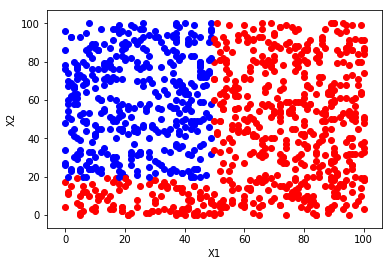
\includegraphics[scale=0.4]{decision_tree_example_data} & \raisebox{.4\height}{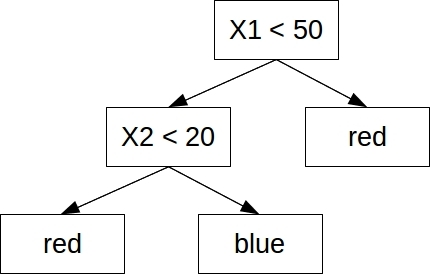
\includegraphics[scale=0.4]{decision_tree_example}}
        \end{tabular}
    \end{center}
    \caption{\label{tab:DecisionTreeExample}Example of Decision Tree}
\end{table}

The algorithms for the construction of decision trees usually work by recursively partitioning the training set $\mathbf{X}$ in such a way that the values of the target vector $\textbf{y}$ are grouped together, until all partitions are composed by a single label. The problem with these building methods is that they produce very complex trees that overfit the training data. Overfitted trees not only lead to poor predictive capabilities on non-training data, but also produce models that can be exceedingly difficult to interpret. A common approach to avoid overfitting in decision trees is to force an early stopping of the algorithm before the tree becomes too complex. Popular stopping criteria include limiting the maximum depth of the tree, requiring a minimum number of sample points at leaf nodes, or computing the accuracy gain yielded by adding new nodes. However, those heuristics demand the optimization of hyperparameters which makes the training process computationally expensive.

    {\color{red} TODO: briefly describe bagging, random forests, and boosting [...] produce multiple trees which are then combined to yield a single consensus prediction [...] combining a large number of trees can often result in dramatic improvement in prediction accuracy, at the expense of some loss of interpretability [...]}

% Subsection: Time Series

\subsection{Time Series Analysis}
\label{sec:intro_time_series}

A time series is a sequence of measurements taken at successively equally spaced points in time, so there exists a natural ordering of the observations. Examples of time series include the daily closing prices of the Standard and Poor's 500 index, the monthly number of passengers of an airline, or the yearly gross domestic product of a particular country. Time series forecasting refers to the process of building a model to predict future values of the series based on the previously observed values. The observed values could be continuous, discrete or even categorical.

{\color{red} Time series are analysed to understand the past and to predict the future [...] A time series analysis quantifies the main features in data and the random variation [...] When a variable is measured sequentially in time over or at a fixed interval, known as the sampling interval, the resulting data form a time series [...] we take a statistical approach in which the historical series are treated as realizations of sequences of random variables [...] referred to as a discrete-time stochastic process [...] The main features of many time series are trends and seasonal variations that can be modelled deterministically with mathematical functions of time. Another important feature of most time series is that observations close toghether in time tend to be correlated (serially dependent) [...] Once a good model is found and fitted to data, the analyst can use the model to forecast future values [...] Fitted models are also used as a basis for statistical tests. [...] Finally, a fitted statistical model provides a concise summary of the main characteristics of a time series. [...] The data may have been aggregated [...] or sampled [...] If data are sampled, the sampling interval must be short enough for the time series to provide a very close approximation to the original continuous signal when it is interpolated [...] a systematic change in a time series that does not appear to be periodic is known as a trend. [...] A repeating pattern [...] within any fixed period [...] is known as seasonal variation [...] cycles [...] do not correspond to some fixed natural period. [...] Forecasting relies on extrapolation, and forecast are generally based on assumption that present trends continue. We cannot check this assumption in any empirical way. [...] ouliers and erroneous vales [...] need to be handled differently in the analysis and must not be included as observation when fitting a model to data. [...] it may be appropiate to consider robust methods of fitting models, which reduce the influence of outliers. [...] it is usually appropiate to remove trends and seasonal effects before comparing multiple series. [...] trend [...] change direction in unpredictable times [...] stochastic trend [...] two unrelated time series will be correlated if they both contain a trend.}

\begin{definition}
    A \emph{time series} of length $n \in \mathbb{N}$, denoted by $\{ x_t : t=1, \ldots, n \}$ or $\{ x_t \}$, is a sequence $\{ x_1, x_2, \ldots, x_n \}$.
\end{definition}

The elements $x_i$ of the series correspond to values sampled at disrete times $1, 2, \ldots, n$, and they can be continuous or categorical. In statistics, a time series is usually modeled as a sequence of $n$ random variables, and a particular time series is a realization of the model. In this sense, $\{ x_t \}$ could represent a collection of random variables or the numerical observations of these random variables.

{\color{red} We represent a time series of length $n$ by $\{ x_t : t=1,\ldots,n \} = \{x_1, x_2, \ldots, x_n \}$. It consists of $n$ values sampled at discrete times $1, 2, \ldots, n$. The notation will be abbreviated to $\{x_t\}$ when the length $n$ of the time series do not need to be specified. The tiem series model is a sequence of random variables, and the observed time series is considered a realizatin of the model.
}

{\color{red} The 'hat' notation will be used to represent a prediction or forecast. For example, with the series $\{ x_t : t=1,\ldots,n \}$, $\hat{x}_{t+k \mid t}$ is a forecast made at time $t$ for a future value at time $t+k$. A forecast is a predicted future value, and the number of time steps into the future is the lead time $k$ [...]
}

\subsubsection{Trends and Seasons}

Many time series ... and a repeating seasonal component.

\begin{definition}
    Let $\{ x_t \}$ be a time series, a \emph{simple additive model} is defined as
    \[
        x_t = m_t + s_t + z_t
    \]
    where $m_t$ is called the \emph{trend component}, $s_t$ is the \emph{seasonal component}, and $z_t$ is the \emph{error term}.
\end{definition}

If the time series presents the property that the seasonal component increases as the trend increases, it might be better to use a multiplicative model.

\begin{definition}
    Let $\{ x_t \}$ be a time series, a \emph{simple multiplicative model} is defined as
    \[
        x_t = m_t \dot s_t + z_t
    \]
    where $m_t$ is called the \emph{trend component}, $s_t$ is the \emph{seasonal component}, and $z_t$ is the \emph{error term}.
\end{definition}

In practice, a simple approach of estimating the trend of a tiem series is to compute a moving average.

\begin{definition}
    Let $\{ x_t \}$ be a time series, a \emph{simple moving average} of lenth $l$ is 
\end{definition}

The best results are achieved when the length $l$ of the moving average is equal to the length of the seasonal component. The seasonal componet can be estimated by

\begin{definition}
    Additive
    \[
        \hat{s}_t = x_t - \hat{m}_t
    \]
    Multiplicative
    \[
        \hat{s}_t = \frac{x_t}{\hat{m}_t}
    \]
\end{definition}


{\color{red} [...] many series are dominated by a trend and/or a seasonal effect [...] A simple additve decomposition model is given by
\[
    x_t = m_t + s_t + z_t
\]
where, a time $t$, $x_t$ is the observed series, $m_t$ is the trend, $_t$ is the seasonal effect, and $z_t$ is an error terms that is, in general, a sequence of correlated random variables with mean zero.

If the seasonal effect tends to increase as the trend increases, a multiplicative model may be more appropriate
\[
    x_t = m_t \dot s_t + z_t
\]

}

\begin{definition}
    \
\end{defintion}

{\color{red} Once we have identired any trend and seasonal effects, we can deseasonalise the time series and remove the trend. If we use the additive decomposition method, we first calculate the seasonality adjusted time series and then remove the trend by substraction. This leaves the random component, but the random component is not necessarily well modelled by independent random variables. In many cases, consecutive variables will be correlated. If we identify such correlations, we can improve our forecast, quite dramatically if the correlations are high.}

\subsubsection{Second Order Properties}

%
% Minimum Message Length
%
\section{Minimum Message Length}
\label{sec:MML}

The \emph{Minimum Message Length} (MML) is based on the idea that a good theory, or explanation, for a dataset is a small collection of premises under which the data is not surprising. The best theories are those which are short, able to explain most of the data, and with a high accuracy. An \emph{explanation message} is composed by two parts: the fist part comprises all the premises induced from the data, including numerical values; the second part contains all the data that cannot be derived from the premises. The message also assumes the existence of some already known and accepted premises (prior knowledge). Given the prior premises and the message it should be possible to recover the original dataset. According to the MML, theories are not rejected due to contradictory measurements, they only make the second part of the message longer.

In the MML principle, a message is a lossless encoded version of the original data. The first part of the message contains a probabilistic model about the data, and the second part is the data encoded using this model. We are interested in finding the shortest possible explanation message. If the length of the explanation message is longer than the original data, the theory is considered unacceptable.

Bayes' theorem (see Theorem \ref{th:bayes}) states that the probability $P(H \mid E)$ of a hypothesis $H$ given an evidence $E$ is:
\[
    P(H \mid E) = \frac{ P( E \mid H ) P(H) }{ P(E) }
\]
We are interested in finding the hypothesis $H$ with the highest posterior probability $P(H \mid E)$ of being true, assuming a fixed evidence $E$. That is, we are looking for maximize $P( E \mid H ) P(H)$ or, equivalently, maximize $P ( H \wedge E )$.

The \emph{Minimum Message Length} principle (MML for short) is based on the idea that the length of encoding $H \wedge E$ as a binary string using an optimal code is equal to $- \log_2 P ( H \wedge E )$ (see Theorem \ref{th:optimal_codes}). That is:
\[
    l(H \wedge E) = - \log_2 P ( H \wedge E ) = - \log_2 P( E \mid H ) P(H) = - \log_2 P( E \mid H ) - \log_2 P(H)
\]
The most probable model $H$ would be that model that allows us to encode $H \wedge E$ with the shortest possible string. The encoded string would be composed by two parts, a general assertion about the data, and a detailed description of the data assuming that the assertion is true.

Let $\mathbb{X}$ be a discrete set composed by all possible datasets, $\mathcal{X}$ a random variable taking values on $\mathbb{X}$, and $f(X \mid \theta)$ a probability distribution for $\mathcal{X}$ given the parameter $\theta$.

\begin{definition}
    Let $\Theta$ be a discrete set of possibles parameters for $f$ with probability distribution $h(\theta) \, \theta \in \Theta$, and let $\hat\theta \in \Theta$ be an inferred parameter. An \emph{assertion} is the encoded version of $\hat\theta$ using an optimal code given the probability distribution $h$.
\end{definition}

The length of the assertion given an optimal binary code is $- \log_2 h(\hat\theta)$ (see Section {\ref{sec:Optimal-Codes}). Note that $\theta$ could be a single scalar or a vector of values. Moreover, $\theta$ could be related to more than one family of probability distributions $f$.

\begin{definition}
    Let $X \in \mathbb{X}$ be a dataset, and $\hat \theta \in \Theta$ an inferred value for the distribution $f$. A \emph{detail} is the encoded version of $X$ using an optimal code given the probability distribution $f(X \mid \hat\theta)$.
\end{definition}

The length of the detail given an optimal binary code is $- \log_2 f( X \mid \hat\theta )$. That is, the length of the detail is the negative of the log-likelihood of $X$ given $\hat\theta$.

\begin{definition}
    Let $X \in \mathbb{X}$ be a dataset, and $\hat \theta \in \Theta$ an inferred value for the distribution $f$ A \emph{message} for the dataset $X$ given an inference $\hat\theta \in \Theta$ is the concatenation of the assertion for $\hat\theta$ and the corresponding detail for $X$ given $\theta$.
\end{definition}

The length of a message given an optimal binary code is $- \log_2 h \left( \hat\theta \right) - \log_2 f \left( X \mid \hat\theta \right)$. The length of a message allow us, for example, to compare the posterior probabilities of two competing explanations or hypotheses $\hat\theta_1$ and $\hat\theta_2$.

\begin{definition}
    Let $X \in \mathbb{X}$ be a dataset. The \emph{Minimum Message Length} of $X$, denoted by $MML(X)$, is given by:
    \[
        MML(X) = \argmin_{\hat\theta \in \Theta} \left( - \log_2 h \left( \hat\theta \right) - \log_2 f \left( X \mid \hat\theta \right) \right)
    \]

\end{definition}

In practice, the actual messages will not be constructed, since our interest is in the length of the messages, not in their content. It is assumed that the sets $\mathbb{X}$ and $\Theta$ and the functions $f(X \mid \hat\theta)$ and $h(\theta)$ are known a priori, and so, it is not necessary to include them as part of our encoding message.

\begin{example}
    \label{ex:MML}
    Consider an experiment in which we toss a weighted coin $100$ times. Denote by $1$ if we get a face and $0$ a cross, so that each experiment is a binary string of length $100$. Our collection of all possible datasets is $\mathbb{X} = \mathcal{B}^{100}$, $\theta$ is a number in the interval $[0, 1]$, the likelihood $f (X \mid \theta)$ follows a binomial distribution (that is, $f (X \mid \theta) ) = \theta^n (1-\theta)^{100-n}$ where $n$ is the number of faces in $X$), and since we do not know anything about how the coin is weighted, we could assume that $h(\theta)$ is the uniform distribution in the interval $[0, 1]$ (that is, $h(\theta) = 1$ for $\theta \in \Theta$). Under these assumptions, the length of a message for $X$ given an inferred parameter $\hat\theta$ would be:
    \[
        - \log_2 h \left( \hat\theta \right) - \log_2 f \left( X \mid \hat\theta \right) = - n \log_2 \hat\theta - (100-n) \log_2 (1 - \hat\theta)
    \]
    We are interested in finding the value of $\hat\theta$ that minimizes the length of the encoded version of $X$, that is, the minimum message length for $X$.
\end{example}

A Maximum A Posteriori analysis of the experiment in Example \ref{ex:MML} would provide the same inference for $\hat\theta$ than the Minimum Message Length approach. Moreover, given that $h(\theta)$ follows an uniform distribution, a Maximum Likelihood approach would reach exactly the same value for $\hat\theta$.

%
% Minimum Description Length
%
\section{Minimum Description Length}
\label{sec:MDL}

The \emph{Minimum Description Length} (MDL) principle is a reformulation
of the Kolmogorov complexity with the goal to make it applicable to
solve practical problems. MDL explicitly address the two most important
practical limitations of the Kolmogorov complexity: its uncomputability
(in general, the Kolmogorov complexity cannot be computed), and the
large constants involved in the invariance theorem (that makes it
inapplicable to short strings). The approach of MDL to these problems
is to scale down Kolmogorov complexity until it does become applicable:
instead of using general-purpose computer languages, MDL is based
on fixed languages and coding functions.

In contrast to Kolmogorov that states that the complexity of a string
is equal to the length of the shortest program that prints that string,
MDL proposes that our capacity to learn about a string is equivalent
to our ability to compress that string. The idea behind MDL is to
describe a dataset with the help of an hypothesis: the more the hypothesis
fits the data (and here good fit equals learning), the more we can
compress the data given that hypothesis.

In our particular case, we are interested in MDL because it will allow
us to compute the nescience of a topic given a dataset, instead of
requiring a text describing the topic. Thus, given a topic $t$ and
a sample dataset $D=\left\{ x_{1},x_{2},\ldots,x_{n}\right\} $, the
nescience of a particular hypothesis $H$ will be related to the capacity
of that hypothesis to compress the dataset.

MDL comes into two versions, \emph{simplified (two-part code) MDL}
and \emph{refined MDL}. Simplified MDL is easier to understand, and
it will allows us to introduce some important concepts and notation.
The extension of the concept of nescience to datasets will be based
on the refined version of MDL.


    {\color{red} TODO: Explain how this relates to cross entropy}


In this section we are going to introduce the two-part code version
of the minimum description length principle for probabilistic models.

\emph{Given a set of candidate models (a set of probability distributions
    (for example first-order Markov chains) or functions of the same functional
    form (for example the kth degree polynomials)) $\mathcal{H^{\left(\text{1}\right)}},\mathcal{H}^{\left(2\right)},\ldots$
    the simplified,} \emph{two-part version,} \emph{of the} Minimum Description
Length Principle \cite{Gr=0000FC05}\emph{ states that the best point
    hypothesis (a single probability distribution (e.g. a Markov chain
    will all parameters values specified) $H\in\mathcal{H^{\left(\text{1}\right)}}\cup\mathcal{H}^{\left(2\right)}\cup\ldots$
    to explain the data $D=\left(x_{1},\ldots,x_{n}\right)\in\mathcal{X}^{n}$
    is the one that minimizes the sum $L(M)+L(D\mid M)$, where $L(M)$
    is the length (in bits) of the model description, and $L(D\mid M)$
    is the length (in bits) of the data encoded with the help of the hypothesis
    ... there is only one reasonable choice for this code ... the so-called
    Shannon-Fano code ... Each hypothesis $H$ may be viewed as a probability
    distribution over $\mathcal{X}^{n}$. For each such distribution there
    exists a code with length function $L$ such that for all $x^{n}\in\mathcal{X}^{n}$
    we have that $L\left(x^{n}\right)=-\log_{2}P\left(x^{n}\mid H\right)$.
    The quantity $L(M)$ depends on each model.}

\emph{A description of the data ``with the help of'' a hypothesis
    means that the better the hypothesis fits the data, the shorter the
    description will be. A hypothesis that fits the data well gives us
    a lot of information about the data. Such information can always be
    used to compress the data. This is because we only have to code the
    errors the hypothesis makes on the data rather than the full data.}

\emph{The sum of the two description length will be minimized at a
    hypothesis that is quite (but not too) ``simple'', with a good (but
    not perfect) fit.}

The length of the data given the model, that is, \emph{$L(D\mid M)$.}

\[
    -\log P(D)=L_{C}(D)
\]


This choice for C gives a short codelegth to sequences which have
high probability according to (k, ttita) while it gives a high codelength
to sequences with low probability. The codelength thus directly reflects
the goodness-of-fit of the data with respect to (k,tita) measured
in terms of the probability fo D according to (k,tita).

When we say we ``code the data D with the help of probabilistic hypothesis
P'' we mean that we code D using the Shannon-Fano code corresponding
to P.

\[
    L(D\mid P):=-\log P(D)
\]


the code with these lengths is the only one that would be optimal
if P where true. (mention we are only interested in code lengths,
we are not interested in to find the code itself).

For \emph{$L(M)$ we use the standard code for integers.}

\begin{example}
    Markov Chain Hypothesis Selection: Suppose we are given data $D X\textasciicircum{}n$
    where $X=\{0,1\}$. We seek a reasonable model for D that allows us to
    make good predictions of future data coming from the same source.
    We decide to model our data using the cass B o all Markov chains ${[}...{]}$
    we face the problem of overfitting: for a given sequence $D=(x1,...,xn)$,
    there may be a Markov chain P of very high order that fits data D
    quite well but that will behave very badly when predicting future
    data from the same source.
\end{example}

\subsection{Refined MDL}

\emph{In refined MDL, we associate a code for encoding $D$ not with
    a single $H\in\mathcal{H}$ but with the full model $\mathcal{H}$
    ... we design a single one-part code with lengths $\bar{L}\left(D\mid H\right)$
    (called the stochastic complexity of the data given the model). This
    code is designed such that whenever there is a member of (parameter
    in) $\mathcal{H}$ that fits the data well, in the sense the $L\left(D\mid H\right)$
    is small, then the codelenth $\bar{L}\left(D\mid H\right)$ will also
    be small. Codes with this property are called universal codes.}

\emph{There are at least four types of universal codes:}
\begin{enumerate}
    \item \emph{The normalized maximum likelihood (NML) code and its variations.}
    \item \emph{The Bayesian mixture code and its variations.}
    \item \emph{The prequential plug-in code.}
    \item \emph{The two-part code.}
\end{enumerate}
\emph{Refined MDL is a general theory of inductive inference based
    on universal codes that are designed to be minimax, or close to minimax
    optimal. It has mostly been developed for model selection, estimation
    and prediction.}

\section{Multiobjective Optimization}

In the area of \emph{multiobjective optimization} we are interested in solving the following problem:
\begin{align*}
     & \text{minimize}	   \quad \left\{f_1(x), f_2(x), \ldots, f_k(x) \right\} \\
     & \text{subject\;to} \quad x \in S
\end{align*}
where $f_i:\mathbb{R}^n \rightarrow \mathbb{R}$ are two or more objective \emph{objective functions}, and the nonempty set $S \subset \mathbb{R}^n$ is the \emph{feasible region}, whose elements $x=\left( x_1, x_2, \ldots, x_n \right)$ are \emph{decision vectors}. The image of the feasible region $f(S) \subset \mathbb{R}^k$ is called \emph{objective region}, and its elements $z = \left(f_1(x), f_2(x), \ldots, f_k(x) \right)$ \emph{objective vectors}.

In this book we will be dealing with nonlinear multiobjective optimization problems, where at at least one of the objective functions is not linear. Objective functions can be also incommensurable, that is, measured in different units.

An objective vector is optimal if none of its components can be improved without deteriorating at least one of the others. In multiobjective optimization the objective functions are usually conflicting, and so, it does not exist a single solution that is optimal with respect to every objective function.

\begin{definition}
    A decision vector $x \in S$ is Pareto optimal if there does not exists another decision vector $y \in S$ such that $f_i(y) \leq f_i(x)$ for all $i = 1, \ldots, k$ and $f_j(y) < f_j(x)$ for at least one $j$. An objective vector $z \in f(S)$ is Pareto optimal if there does not exits another objective vector $w \in f(S)$ such that $w_i \leq z_i$ for all $i = 1, \ldots, k$ and $w_j < z_j$ for at least one $j$.
\end{definition}

An objective vector is Pareto optimal if its corresponding decision vector is Pareto optimal.

    {\color{red} [...] the Pareto optimal set (consisting of the Pareto optimal solutions) can be nonconvex and disconnected [...]}

    {\color{red} TODO: Add an example}

    {\color{red} [...] in practice, usually only one of these solutions is to be chosen [...] In multiobjective optimization, there are at least two equally important tasks: an optimization task for finding Pareto optimal solutions [...] and a decision-making task for choosing a single most preferred solution}

    {\color{red} [...] putting the preference articulation stage after optimization [...]}

    {\color{red} TODO: Introduce the following concepts: locally Pareto optimal, weak Pareto optimality}

    {\color{red} TODO: Introduce the following concepts: ideal vector (lower bound), nadir (upper bound), utopian}

    {\color{red} TODO: Indroduce the following concept: Decision Maker [...] because Pareto optimal solutions cannot be ordered completely, we need extra preference information coming from a decision maker [...] explicit preference model [...]}

    {\color{red} [...]there is no DN and his preference information available and in those cases we must use so-called no-preference methods. Then, the task is to find some neutral compromise solution without any additional preference information. This means that instead of asking the DM for preference information, some assumptions are made about what a "reasonable" compromise could be}

\subsection{Trade-offs}

{\color{red} [...] a trade-off is an exchange, that is, a loss in one aspect of the problem, in order to gain additional benefit in another aspect [...] a trade-off represents giving up in one of the objectives, which allows the improvement of another objective [...] how much must we give up of a certain objective in order to improve another one to a certain quantity}

{\color{red} objective trade-off vs. subjective trade-off}

{\color{red}

    \begin{definition}
        Let us consider two feasible solutions $x^1$ and $x^2$, and the corresponding objective vectors $f(x^1)$ and $f(x^2)$. Then, the ratio of change between $f_i$ and $f_j$ is denoted by $T_{ij}$
    \end{definition}

}

\subsection{Optimization Methods}

{\color{red} Sometimes, there is no DM and his preference information available and in those cases we must use so-called no-preference methods. Then, the task is to find some neutral compromise solution without any additional preference information. This means that instead of asking the DM for preference information, some assumptions are maked about what a "reasonable" compromise could be like.}

{\color{red} it is important that the multiobjective optimization method used can meet the following two needs: firstly, it must be able to cover, that is, find any Pareto optimal solution, and, secondly, generate only Pareto optimal solutions.}

%
% Section: References
%

\section*{References}

 {\color{red} TODO: Add paper of Turing about AI.}

The minimum message length principle was developed by Chris Wallace, published for first time in 1968 in \cite{wallace1968information}. The book \cite{wallace2005statistical}, written by the same author, contains a detailed description of the principle.



%
% CHAPTER: Philosophy of Science
%

%
% CHAPTER - Philosophy
%

\chapterimage{Philosophers.pdf}

\chapter{Philosophy of Science}
\label{chap:Philosophy}

\begin{quote}
\begin{flushright}
\emph{To go where you don't know, \\
you have to go the way you don't know.} \\
San Juan de la Cruz 
\end{flushright}
\end{quote}
\bigskip

The \emph{philosophy of science}\index{Philosophy of science} is the branch of philosophy that examines the foundations, methods, and implications of scientific inquiry. It explores how scientific knowledge is generated, the validity of scientific theories, the nature of scientific reasoning, and the role of values in science. By addressing fundamental questions about objectivity, reality, and the limits of scientific explanation, the philosophy of science helps us understand how science works and its impact on our understanding of the world.

The philosophy of science provides us a theoretical framework for analyzing the core elements that constitute our theory of nescience. It enables us to critically examine the foundations and assumptions of our theory, guiding us toward the identification of the essential questions that we must address. Moreover, philosophical inquiry compels us to rigorously push the boundaries of our analysis, ensuring that our theory is explored to its ultimate consequences, both logically and conceptually. This approach strengthens the robustness of the theory, even if it these results do not directly translate into practical applications.

In the chapter, we provide a concise overview of key elements from the philosophy of science, as well as relevant concepts from other branches of philosophy, such as metaphysics, epistemology, and ontology, that are important to the theory of nescience. Certain other topics within the philosophy of science, such as the problem of objectivity (examining whether science can be truly objective or is influenced by social and personal values) or the role of values in science, including the relationship between ethical, social, and political values and scientific practices, are not included in this review, as they are not directly relevant to a mathematical theory of nescience.

The chapter begins with a brief introduction to the field and its importance in understanding scientific inquiry. We delve into the problem of which entities can be known, examining the scope of scientific knowledge and the nature of observable and unobservable phenomena. The chapter also addresses the concept of scientific representation, discussing how models, theories, and laws reflect aspects of reality. We examine how science discovers new knowledge, the principles behind the scientific method, and the various ways in which scientists formulate and test hypotheses. Finally, we explore the limits of science, considering the boundaries of what science can explain and where its explanatory power may fall short.

%
% Section: Metaphysics
%

\section{What is Science}

\emph{Science}\index{Science} is a systematic method of investigating the world around us, aimed at generating reliable knowledge through observation and reasoning. Unlike other forms of inquiry, science is rooted in the idea that knowledge must be based on evidence that can be tested and verified. By combining theoretical thinking with empirical data, science offers a powerful way to explain, predict, and understand natural phenomena. The following is a list of the key features that make science distinct and valuable as a way of knowing.

\begin{itemize}

\item \emph{Empiricism}\index{Empiricism}: At its core, science is an empirical endeavor, meaning it relies on observation, experimentation, and measurable evidence to understand the natural world. Scientific knowledge is grounded in data that can be gathered through direct or indirect observation, ensuring that claims can be tested and verified by others.

\item \emph{Testability}\index{Testability}: A key characteristic of science is its focus on developing testable hypotheses, that is, statements or predictions that can be empirically investigated. This means that scientific claims must be falsifiable, open to potential disproof if the evidence does not support them. This distinguishes science from fields that rely on unfalsifiable or speculative claims.

\item \emph{Theoretical Frameworks}\index{Theoretical framework}: Science is not merely about collecting facts; it seeks to develop broader explanations through models, laws, and theories. Models offer simplified representations of complex systems, while theories are well-supported frameworks that explain the underlying mechanisms of phenomena. These frameworks help interpret data and guide further investigation, offering coherence to the body of scientific knowledge.

\item \emph{Self-Correction}\index{Self-correction}: A defining feature of science is its self-correcting nature. Scientific theories are not static; they evolve as new evidence comes to light. When new data contradicts a theory, science adapts, modifies, refines, or sometimes discards the theory in favor of one that better fits the evidence. This continuous process of revision ensures that scientific knowledge becomes more accurate over time.

\item \emph{Generalizability}\index{Generalizability}: Science strives to uncover universal principles that apply across various contexts, not just to isolated cases. While science begins with specific observations, its goal is to identify general laws and patterns that explain a broad range of phenomena. This pursuit of generalizable knowledge allows science to predict future occurrences and provide deeper insights into the workings of the natural world.

\end{itemize}

 \emph{Ontology}\index{Ontology}, the branch of philosophy concerned with the nature of existence, addresses the question of which entities exist in the real world. It examines the types of entities that science can study, whether they are observable, abstract, or indeterminate, and engages with the philosophical debates surrounding their existence. Ontology provides the foundation for exploring the boundaries of scientific knowledge and the limits of inquiry. \emph{Epistemology}\index{Epistemology} is the branch of philosophy concerned with knowledge itself—how we acquire it, what justifies it, and what its limits are. While ontology deals with what exists, epistemology addresses how we come to know what exists. In the context of science, epistemology examines the methods, evidence, and reasoning that underpin scientific investigation, exploring how scientific knowledge is built, how reliable it is, and what counts as a justified belief in scientific practice. Both ontology and epistemology are part of the broader field of \emph{metaphysics}\index{Metaphysics}, which deals with the fundamental nature of reality and existence. Metaphysics explores the most basic concepts and categories of being, such as time, space, causality, and possibility, as well as the relationship between mind and matter. Together, ontology, epistemology, and metaphysics provide a comprehensive philosophical foundation for understanding what science studies, how it builds knowledge, and the fundamental nature of the reality science seeks to explain.


%
% Section: What is an Entity
%

\section{What is an Entity}

In this section, we focus on the fundamental problem of determining which kinds of entities can be known or investigated by science.

\begin{figure}[t]
\centering
\begin{tikzpicture}

  % Define the ovals
  \node[draw, ellipse, minimum width=4cm, minimum height=1.1cm, align=center] (knowable) {Knowable};
  \node[draw, ellipse, minimum width=4cm, minimum height=1.1cm, right=of knowable, xshift=2+1cm] (nonknowable) {Non-Knowable};
  \node[draw, ellipse, minimum width=3.5cm, minimum height=1.1cm, below=of knowable, xshift=-2.5cm] (concrete) {Concrete};
  \node[draw, ellipse, minimum width=3.5cm, minimum height=1.1cm, below=of knowable, xshift=2.5cm] (abstract) {Abstract};
  \node[draw, ellipse, minimum width=3cm, minimum height=1.1cm, below=of concrete, xshift=-2.5cm] (observable) {Observable};
  \node[draw, ellipse, minimum width=3cm, minimum height=1.1cm, below=of concrete, xshift=2.5cm] (nonobservable) {Non-Observable};

  % Arrows indicating subset relationships
  \draw[<-] (concrete) -- (knowable) node[midway, left] {};
  \draw[<-] (abstract) -- (knowable) node[midway, right] {};
  \draw[<-] (observable) -- (concrete) node[midway, left] {};
  \draw[<-] (nonobservable) -- (concrete) node[midway, right] {};

\end{tikzpicture}
\caption{Classification of Research Entities}
\end{figure}

A \emph{knowable entity}\index{Knowable entity} is an object, phenomenon, or concept that can be investigated, understood, or described through scientific or intellectual inquiry. Knowable entities are those that, either directly or indirectly, can be observed, measured, inferred, or modeled, using available tools, methods, or theories. They are within the scope of human knowledge, and their properties can be analyzed or explained. Examples of knowable entities include the stars and plantes, animals, or computer algorithms. A \emph{non-knowable entity}\index{Non-knowable entity} refers to something that cannot be directly observed, measured, or understood using current scientific or intellectual methods. This could be due to limitations in technology, the abstract or metaphysical nature of the entity, or inherent epistemological boundaries. Non-knowable entities might remain beyond the reach of human understanding either temporarily (until methods evolve) or permanently (due to their nature). Examples of non-knowable entities include the nature of consciousness, the origin of the universe, or the existence of a deity. The distinction between knowable and non-knowable entities is not always fixed, but varies depending on the clarity and precision of the area of interest and the evolving nature of scientific understanding in each field.

Scientific research encompasses both \emph{concrete entities}\index{Concrete entities} and \emph{abstract entities}\index{Abstract entities}. Concrete entities refer to physical objects or phenomena that can be directly observed, measured, or interacted with, such as stars, cells, or chemical compounds. These entities form the basis of empirical research, where data is collected through direct observation or experimentation. In contrast, abstract entities are conceptual and do not have a physical presence, such as numbers, algorithms, or theoretical models. Abstract entities play a crucial role in scientific research, particularly in fields like mathematics and theoretical physics, where they provide the framework for understanding and modeling concrete phenomena. While abstract entities cannot be observed directly, they can be known through indirect methods. The inclusion of these abstract entities in scientific inquiry raises important philosophical questions about their ontological status: Are these abstract entities real in the same way that physical objects are, or are they simply conceptual tools? This question remains an open and debated issue in the philosophy of science.

Finally, in scientific inquiry, there is also a distinction between \emph{observable entities}\index{Observable entities}, which can be directly perceived or measured, and \emph{non-observable entities}\index{Non-observable entities}, which are inferred from empirical evidence but cannot be directly observed. Observable entities include things like trees, planets, and bacteria—objects that can be seen or detected using scientific instruments. Non-observable, but still concrete, entities include things like subatomic particles and gravitational forces. These entities are often crucial for explaining observable phenomena but exist at a level beyond direct human perception. For example, we cannot observe an electron in the same way we observe a tree, but through scientific theory and experimentation, we infer its existence.

A central debate within the scope of science is the tension between \emph{reductionism}\index{Reductionism} and \emph{holism}\index{Holism}. Reductionism is the view that complex systems can be fully understood by breaking them down into their simplest, most fundamental parts. For example, a reductionist might argue that biological processes can be explained entirely by chemistry, and chemistry by physics. This approach assumes that understanding the smallest components of a system will provide a complete explanation of the whole. In contrast, holism argues that some phenomena cannot be fully understood by reducing them to their components. Instead, the whole system exhibits properties that cannot be predicted or explained by analyzing its parts in isolation. For example, in ecology, the interactions within an ecosystem can produce emergent properties that are not reducible to the behavior of individual species.

Finally, the scope of science is shaped by the debate between \emph{scientific realism}\index{Realism} and \emph{anti-realism}\index{Anti-realism}, which addresses the question of whether the entities posited by scientific theories are real or merely useful constructs. Scientific realism holds that the entities described by scientific theories—whether observable or not—exist independently of our knowledge of them. According to this view, successful scientific theories reveal truths about the world. In contrast, anti-realism (or \emph{instrumentalism}\index{Instrumentalism}) argues that scientific theories are useful tools for predicting and organizing observations, but we should not necessarily believe that unobservable entities like electrons or gravitational waves are real. For anti-realists, the purpose of science is not to describe an independent reality, but rather to provide models that help us navigate and predict phenomena. This ontological uncertainty leads to philosophical discussions about \emph{natural kinds}\index{Natural kinds}—whether the categories used in science reflect real, essential divisions in nature, or whether they are human-made constructs imposed to bring order to a complex and often ambiguous reality. 

%
% Scientific Representation
%

\section{Scientific Representation}
\label{sec:scientific_representation}

Science helps us understand the natural world by using different kinds of representations of research entities. These representations include measurements from scientific instruments, descriptions of observations, digital images like X-rays or MRI scans, and more. Scientific practice also often considers mathematical equations, models, and theoretical constructs as valid forms of representation. The challenge of \emph{scientific representation}\index{Scientific representation} is to identify the conditions that make a representation scientific and determine what makes an effective representation. The main issues discussed in this area of philosophy include:

\emph{Scientific Representation Problem}: The scientific representation problem is about figuring out the necessary and sufficient conditions that make a representation valid in science. It explores whether these conditions are the same across all scientific fields or if they vary depending on the discipline or research context. For example, what qualifies as a valid representation in physics, which often uses mathematical models, might be different from what is used in biology, where visual and descriptive representations are common. This problem also questions whether scientific representations need to be adapted to specific research goals to be considered valid.

\emph{Representational Demarcation Problem}\index{Representational demarcation}: The representational demarcation problem looks at whether scientific representations are fundamentally different from other kinds of representations, like those found in art or everyday life. It examines what makes scientific representations unique, focusing on their purpose, accuracy, and the methods used to create them. Unlike artistic representations, which may emphasize subjective interpretation or aesthetic value, scientific representations are generally held to standards of precision, reliability, and empirical adequacy. Understanding these differences helps clarify the specific role that scientific representations play in knowledge production.

\emph{Problem of Style}\index{Problem of style}: The problem of style addresses the fact that the same entity can be represented in different ways, depending on the goals and methods of the research. Different styles of representation—such as diagrams, mathematical equations, physical models, or computer simulations—each have unique characteristics, including the intended audience, level of abstraction, and type of information conveyed. This issue also asks whether these styles are fixed or if new styles can be invented to meet emerging scientific needs. The flexibility of representation styles is crucial because it allows for new insights and different ways of understanding scientific phenomena.

\emph{Standard of Accuracy}\index{Standard of accuracy}: The standard of accuracy problem is about determining what makes a scientific representation accurate. It involves figuring out how to distinguish between accurate and inaccurate representations by considering factors like how well the representation matches empirical data, captures important features of the phenomenon, and its ability to make predictions. This issue also explores whether accuracy should be seen as an objective standard or if it depends on the specific aims and context of the research. For example, a simplified model might still be considered accurate if it effectively serves its purpose, such as making predictions or providing explanations.

\emph{Problem of Ontology}\index{Problem of ontology}: The problem of ontology in scientific representation deals with the nature of the entities that can serve as representations. It asks whether representations need to be concrete, like physical models or graphs, or if they can also be abstract, like mathematical equations or theoretical constructs. This issue also questions whether representations must be realistic or if more abstract, idealized forms can still be effective in scientific inquiry. Understanding these ontological aspects helps define the types of entities that are allowed in scientific discourse and how they relate to the real-world phenomena they represent.

There are also five conditions of adequacy that a scientific representation should satisfy to be considered effective and reliable:

\emph{Requirement of Directionality}\index{Requirement of directionality}: The requirement of directionality examines the relationship between representations and the real world. Representations are meant to describe entities in the real world, but this condition raises the question of how, if at all, real-world entities might describe their representations. It challenges us to think about the direction of influence between the representation and the entity it aims to depict.

\emph{Surrogative Reasoning}\index{Surrogative reasoning}: Surrogative reasoning addresses how scientific representations allow researchers to generate hypotheses about the entities they represent. This condition explores how using a representation as a surrogate can lead to new insights or predictions about the target, effectively using the representation to stand in for the real-world entity during reasoning and analysis.

\emph{Applicability of Mathematics}\index{Applicability of mathematics}: The applicability of mathematics condition is concerned with how mathematical models can be used to represent the real world. It questions how abstract mathematical constructs can effectively describe complex physical systems and whether the success of mathematical representation depends on any special features of the target phenomena. This condition highlights the central role of mathematics in developing and understanding scientific theories.

\emph{Possibility of Misrepresentation}\index{Possibility of misrepresentation}: The possibility of misrepresentation addresses whether representations that are not fully accurate can still be considered valid scientific representations. It considers situations where simplifications or approximations are necessary and whether these less-than-perfect representations can still contribute valuable understanding of a phenomenon. This condition is important for understanding how idealizations and abstractions function in scientific practice.

\emph{Targetless Models}\index{Targetless models}: The targetless models condition explores whether we can allow representations that do not have a direct real-world counterpart. It questions if a model that does not represent any existing entity can still be useful in scientific inquiry, perhaps as a way to explore theoretical possibilities or to understand potential scenarios. This condition emphasizes the creative and exploratory aspects of scientific modeling.

There have been multiple proposals to formally define the concept of scientific representation. Unfortunately, none of these proposals can provide a convincing answer to the questions and conditions of adequacy described above. In the rest of this section, we describe some of these proposals, identifying their advantages and drawbacks. To compare these proposals, we will present them as: "A scientific model $M$ represents a target system $T$ if, and only if ...".

\emph{Stipulative Fiat}\index{Stipulative fiat}: The stipulative fiat proposal states that "a scientific model $M$ represents a target system $T$ if, and only if, a scientist stipulates that $M$ represents $T$." The main problem with this interpretation is that, since anything can be a representation if a scientist says so, it is difficult to guarantee the surrogative reasoning condition. If any model can be deemed a representation by simple stipulation, it becomes challenging to determine which representations are genuinely useful for making scientific inferences. Proponents of this theory acknowledge that while all representations may be stipulated, some are undeniably more useful than others.

\emph{Similarity Conception}\index{Similarity conception}: The similarity conception proposes that "a scientific model $M$ represents $T$ if, and only if, $M$ and $T$ are similar." This conception addresses the surrogative reasoning condition since similarity between the model and the target allows us to derive similar properties. However, it introduces new challenges, particularly regarding the problem of style. The concept of similarity is often vague: in what sense are $M$ and $T$ similar? This vagueness can lead to issues with directionality and accuracy, as different aspects of similarity may not always align with what is relevant for scientific representation.

\emph{Structuralist Conception}\index{Structuralist conception}: The structuralist conception is based on the idea of isomorphism. According to this view, a scientific model $M$ represents a target system $T$ if the structure of $M$ is isomorphic to the structure of $T$. In other words, there is a one-to-one correspondence between the elements and relationships in both $M$ and $T$. This approach justifies surrogative reasoning because having the same structure implies that properties and relations in the model correspond to those in the target. Furthermore, since mathematics is fundamentally concerned with the study of structures, this conception also supports the applicability of mathematics in representing natural systems.

\emph{Inferential Conception}\index{Inferential conception}: The inferential conception proposes that a model $M$ is an epistemic representation of a target $T$ if, and only if, the user adopts an interpretation of $M$ in terms of $T$. This view emphasizes the role of the user in giving meaning to the model, suggesting that representation is not an inherent property of the model itself but arises through its use in making inferences about the target system. This conception underscores the importance of context and interpretation in determining whether a model effectively represents its target.

\emph{Fiction View of Models}\index{Fiction view of models}: According to the fiction view of models, $M$ represents $T$ if and only if $M$ functions as a prop in a game of make-believe that prescribes imagining certain things about $T$. This view draws an analogy between scientific modeling and storytelling, where models are treated as fictional constructs that facilitate imaginative engagement with the target system. Although this approach highlights the creative aspects of modeling, it raises questions about how such fictional constructs can be rigorously linked to real-world entities.

\emph{Representation-As}\index{Representation-as}: The representation-as approach suggests that a scientific model represents a target system as something, emphasizing that representation involves highlighting certain features of the target while downplaying others. This conception focuses on the interpretive aspect of modeling, where the modeler selects specific attributes of the target to represent, depending on the research goals. This approach allows for a flexible understanding of representation that can accommodate different styles and purposes, but it also implies that the usefulness of a representation is contingent on how well the modeler captures the relevant aspects of the target.

Each proposal has its strengths and weaknesses, highlighting the complexity of what it means for a model to effectively represent a target in scientific inquiry. Understanding these various perspectives is crucial for advancing our comprehension of the role of representation in science.


%
% Scientific Explaination
%

\section{Scientific Explaination}

The assumption often made is that there exists a single, distinct type of explanation that qualifies as "scientific." The concept of "scientific explanation" suggests at least two key distinctions: first, a contrast between explanations characteristic of science and those that are not, and second, a contrast between "explanations" and other forms of discourse, such as mere "descriptions." It is important to note that a set of claims can be true, accurate, and supported by evidence while still failing to qualify as explanatory. Scientific explanations primarily aim to clarify why things happen, whether these "things" are particular events or more general phenomena. Central to this discussion are interrelated concepts such as "explanation," "law," "cause," and "support for counterfactuals," all of which share a "modal" character. However, explaining one of these concepts using others from the same family is often considered "circular"; instead, they must be elucidated through concepts external to this modal framework. Additionally, a significant question arises regarding whether all scientific explanations are inherently causal, and if not, what precisely distinguishes causal explanations from non-causal ones.

The \emph{Deductive-Nomological model}\index{Deductive-Nomological model}, or DN model, emphasizes the importance of deductive reasoning and general laws. According to this model, a phenomenon is explained by demonstrating how it logically follows from a general law combined with specific initial conditions. This an explanation comprises two main components: the \emph{explanans}\index{explanans}, which includes the general laws and initial conditions, and the \emph{explanandum}\index{explanandum}, which is the phenomenon to be explained. For the explanation to be valid, the explanans must be true and logically entail the explanandum, meaning the phenomenon can be deduced from the laws and conditions provided. A DN model answers the question "Why did the explanandum occur?" by showing that the phenomenon resulted from specific circumstances $C_1, C_2, \ldots, C_i$, in conjunction with laws $L_1, L_2, \ldots, L_j$. For example, the motion of a pendulum can be explained by applying Newton's laws of motion (general laws) along with specific details such as the pendulum's length and initial displacement.

The \emph{Statistical-Relevance model}\index{Statistical-Relevance model}, or SR model focuses on explaining phenomena through statistical relationships rather than strict deductive reasoning. Unlike the Deductive-Nomological model, which requires logical entailment from general laws, the SR model emphasizes the identification of statistically relevant factors that significantly influence the likelihood of a phenomenon. In this model, given some class or population \( A \), an attribute \( C \) is \emph{statistically relevant}\index{Statistical relevance} to another attribute \( B \) if and only if \( P(B | A, C) \neq P(B | A) \). This means that \( C \) affects the probability of \( B \) within the context of \( A \). An explanation involves identifying such statistically relevant factors and evaluating their impact within a reference class (a group of events or entities sharing common characteristics). For example, in explaining the likelihood of developing a particular disease, an SR explanation might highlight factors such as age, genetic predisposition, or lifestyle choices, showing how these variables alter the probability of the disease occurring. By uncovering these statistical relationships, the SR model provides a method for explaining probabilistic phenomena that cannot be addressed deterministically.

The \emph{Causal-Mechanical model}\index{Causal-Mechanical model}, or CM model, of scientific explanation emphasizes understanding phenomena by uncovering the underlying causal mechanisms that produce them. This model asserts that explanations are not just about identifying laws or statistical relationships but about revealing the actual processes and interactions that link causes to effects. A causal-mechanical explanation requires tracing a continuous causal chain, often through detailed physical or biological processes, to show how an event is brought about. For example, explaining the boiling of water involves identifying the causal mechanism: heat energy transfers to the water molecules, increasing their kinetic energy until intermolecular bonds are overcome, leading to a phase change from liquid to gas. The CM model prioritizes clarity in how individual components interact and influence each other, providing a deeper understanding of the phenomenon by grounding it in observable and empirically testable mechanisms. This approach is particularly effective in fields like biology, physics, and engineering, where complex systems and their interactions play a central role in explanation.

The \emph{unificationist account}\index{Unificationist account} of scientific explanation, emphasizes the power of explanation through the unification of diverse phenomena under a single, coherent framework of principles and patterns. According to this model, the primary aim of scientific explanation is to reduce the number of independent assumptions and derive a wide range of phenomena from a minimal, consistent set of explanatory patterns. An explanation is considered successful if it contributes to this unifying framework by connecting seemingly disparate observations through common principles. For instance, Newtonian mechanics unifies the motions of celestial bodies and terrestrial objects under the same laws of motion and gravitation. The unificationist approach highlights the importance of simplicity, generality, and coherence in scientific theories, proposing that the value of an explanation lies in its ability to integrate knowledge into an organized, explanatory schema. By offering a comprehensive understanding of diverse phenomena, this account showcases the interconnectedness and systematic nature of scientific inquiry.

The \emph{pragmatic theories}\index{Pragmatic theories} of scientific explanation emphasize the context-dependent and audience-specific nature of explanations, focusing on their purpose and practical utility rather than strict formal structures. These theories argue that explanations are answers to "why" questions posed within a specific context, and their adequacy depends on how well they address the interests and background knowledge of the audience. A scientific explanation, therefore, is not inherently tied to a universal standard but varies depending on the explanatory goals, such as prediction, understanding, or control. For instance, explaining why a bridge collapsed might involve detailed structural analysis for engineers, whereas a simplified account focusing on the immediate cause, like high winds, might suffice for the general public. Pragmatic approaches recognize that explanatory demands can differ across disciplines, situations, and audiences, making the effectiveness of an explanation contingent on its relevance, clarity, and alignment with the inquirer's needs. This perspective underscores the interplay between scientific knowledge and its communication within varied practical contexts.


%
% The Scientific Method
%

\section{The Scientific Method}

The \emph{scientific method}\index{Scientific method} is understood as the systematic process by which science acquires new knowledge. In schools, the scientific method is often taught as a series of steps: first observing and describing a phenomenon, then coming up with a hypothesis to explain it, testing that hypothesis through experiments, analyzing the data, and finally making a conclusion. However, the idea of a single, universal scientific method isn’t widely accepted anymore. Instead, scientists and philosophers recognize that different scientific fields require different methods because each field faces its own challenges and complexities.

A major idea in scientific methodology is the difference between \emph{discovery}\index{Scientific discovery} and \emph{justification}\index{Scientific justification}. Discovery is about how new ideas or hypotheses come to life, which often happens through creativity, intuition, or even by accident. Justification, on the other hand, is about using evidence and logical reasoning to evaluate these ideas and decide if they are valid. Most philosophers of science have focused more on justification, looking at ways to carefully test and analyze ideas rather than on the less structured processes involved in creating them.

% Scientific Discovery
\subsection{Scientific Discovery}

Scientific discovery refers to the process through which new knowledge, ideas, or principles are uncovered within science. Unlike the systematic procedures associated with justification, discovery often involves creativity, intuition, and inspiration. While some discoveries arise from planned experiments or systematic observation, others occur unexpectedly, challenging existing paradigms or opening new fields of inquiry. The general agreement among philosophers is that the creative process of conceiving a new idea is a non-rational process that cannot be formalized as a set of steps. Understanding discovery is crucial for appreciating how science evolves and adapts, as it reveals the dynamic and often unpredictable nature of scientific progress.

The following two proposals assume that a domain-neutral logic of discovery can be formalized, offering attempts to develop such a framework.

\begin{itemize}

\item \emph{Discovery as abduction}\index{Abductive reasoning}: Abductive reasoning is a mode of discovery that begins with surprising or anomalous phenomena and seeks to generate plausible hypotheses to explain them. This process is conceptualized as follows: (i) some unexpected data, such as $p_1, p_2, \ldots, p_n$, is encountered; (ii) these data would be less surprising if a hypothesis of type $H$ were true; and (iii) therefore, there is justification to develop a hypothesis of type $H$. Two types of abduction are distinguished: \emph{selective abduction}, which involves choosing from known hypotheses, and \emph{creative abduction}, which generates entirely new hypotheses. Abduction present some limitations. First, multiple hypotheses may explain the same phenomena, making additional criteria necessary to evaluate their merit. Second, the schema of abductive reasoning does not account for the act of conceiving a hypothesis itself.

\item \emph{Heuristic programming}\index{Heuristic programming} is a computational approach designed to simulate and assist the creative aspects of human problem-solving. These programs operate as searches within a defined problem space, which includes all possible configurations for a given domain. Each configuration represents a specific state within the problem space, with two key states being the initial state, the starting point of the search, and the goal state, which represents the desired outcome. Operators define the moves that transition between states, while path constraints limit permissible moves within the problem space. Problem-solving in this context involves finding a sequence of operations that connects the initial state to the goal state. The core aim of this approach is to develop heuristics (practical rules or strategies) to efficiently navigate and solve complex problems. Heuristic programming has its limitations, scientific problem spaces are often ill-defined, and computer programs rely on experimental data, meaning that simulations frequently cover only specific aspects of scientific discovery.

\end{itemize}

Many philosophers argue that discovery is an important topic within the philosophy of science, even as they move away from the idea of a formal logic of discovery. A highly influential perspective is Thomas Kuhn's examination of how new facts and theories emerge in the so-called \emph{paradigm shifts}\index{Paradigm shift}. According to Kuhn, discovery is not a single event but rather a complex and prolonged process that often results in paradigm shifts. Paradigms consist of shared generalizations, theoretical commitments, values, and exemplars that unify a scientific community and shape its research practices. During periods of normal science, research focuses on expanding and refining the existing paradigm rather than pursuing novelty. Discovery typically begins with the recognition of anomalies—phenomena that defy the expectations established by the current paradigm. This process includes observing and conceptualizing the anomaly, followed by revising the paradigm to accommodate it. During paradigm crises, theory-driven discoveries may occur as scientists propose speculative theories, develop new expectations, and conduct experiments or observations to test these ideas. Ultimately, a new paradigm emerges, transforming the once-anomalous phenomena into standard expectations.

{\color{red} Others argue that discovery is governed by a methodology. The methodology of discovery is a legitimate topic for a philosophical analysis.}

\begin{itemize}

\item Discoverability

\item Preliminary apprisal

\item Heuristic strategies

\end{itemize}

Finally, scientific discovery can be also viewed as inherently tied to creativity, with philosophers drawing from cognitive science, neuroscience, computational research, and environmental and social psychology to better understand how new ideas emerge. This perspective aims to demystify the mental processes behind creative thought, emphasizing that scientific creativity can be analyzed and understood philosophically. Central to this analysis are two pivotal cognitive mechanisms: analogies and mental models, which serve as fundamental tools in the generation of innovative ideas and the advancement of knowledge.

\begin{itemize}

\item \emph{Analogy}\index{Analogy}: Analogies play a crucial role in scientific discovery by enabling the transfer of ideas from one domain to another. Philosophers distinguish between three types of analogies: positive, negative, and neutral. Positive analogies involve properties that are shared by both the model (the well-understood domain) and the target domain (the new domain). Negative analogies include properties that belong solely to the model and do not apply to the target domain. Neutral analogies are the most intriguing because they consist of properties whose relevance to the target domain remains uncertain. These neutral analogies are significant as they often lead to new insights and hypotheses about the less familiar domain. Additionally, there is a distinction between horizontal and vertical analogies. Horizontal analogies connect two domains at the same level of abstraction, whereas vertical analogies involve relationships between different levels of abstraction within the same domain.

\item \emph{Model-based reasoning}\index{Model-based reasoning}: The concept of model-based reasoning suggests that much of human thought, including probabilistic and causal reasoning as well as problem-solving, relies on mental models rather than formal logic or strict methodological rules. In this approach, the mind constructs structural representations of real-world or imagined situations and manipulates these models to explore possibilities and generate insights. Conceptual structures are viewed as models, and conceptual innovation involves creating new models using various operations. Analogical reasoning, or analogical modeling, is one of the primary forms of model-based reasoning, alongside visual modeling and simulative modeling, such as through experiments.

\end{itemize}

% Scientific Justification
\subsection{Scientific Justification}

Thomas Kuhn introduced the concept of scientific paradigms, which revolutionized the understanding of scientific progress. A paradigm encompasses the set of practices, theoretical frameworks, methodologies, and standards that define a scientific discipline during a specific period. According to Kuhn, normal science operates within the confines of a prevailing paradigm, solving puzzles and extending the framework. However, scientific revolutions occur when anomalies accumulate—phenomena that the existing paradigm cannot adequately explain—leading to a paradigm shift. This shift replaces the old framework with a new one that better accommodates the observed data, fundamentally altering the trajectory of scientific inquiry. Kuhn's insights emphasize the sociocultural and historical dimensions of science, challenging the notion of continuous, cumulative progress.

Paul Feyerabend, in his provocative work "Against Method," argued that there is no universal scientific method that guarantees the success of science. He criticized the rigid methodological rules proposed by philosophers like Popper and Kuhn, suggesting that science has advanced precisely because of its methodological anarchy. Feyerabend contended that "anything goes" in science, meaning that historical scientific breakthroughs often occurred by defying established rules and norms. For example, Galileo's use of persuasive rhetoric and creative reasoning, rather than strict adherence to empirical observation, was crucial in advancing heliocentrism. Feyerabend's ideas challenge the assumption that scientific progress is orderly and rational, emphasizing instead the role of historical, cultural, and personal factors in shaping scientific practice. While his views remain controversial, they highlight the complexity and diversity of scientific inquiry and question the feasibility of prescribing universal methodological principles.

The hypothetico-deductive method is a widely recognized approach in the philosophy of science, describing how scientific theories and knowledge are developed and tested. It begins with the formulation of a hypothesis, which serves as a tentative explanation for a phenomenon or a set of observations. From this hypothesis, scientists deduce specific, testable predictions or consequences, often in the form of "if-then" statements. These predictions are then subjected to empirical testing through experiments or observations. If the results align with the predictions, the hypothesis is supported but not conclusively proven; if the results contradict the predictions, the hypothesis may need to be revised or rejected. This iterative process underscores the provisional nature of scientific knowledge.

Falsificationism emphasizes that scientific theories can never be conclusively proven but can be rigorously tested through attempts to falsify them. An example of this is Einstein's theory of general relativity, which predicted that light would bend near massive objects like the sun. This prediction was empirically tested during the solar eclipse of 1919, when astronomers observed starlight bending as it passed near the sun, providing a crucial opportunity to potentially falsify the theory—but instead offering strong support for it. According to this perspective, a theory is scientific only if it is falsifiable—that is, if it makes predictions that could, in principle, be shown to be false by empirical evidence. In this view, the strength of a scientific theory lies in its ability to withstand attempts at falsification, and progress in science occurs when falsified theories are replaced by better, more robust ones. This perspective shifts the focus from verification to critical testing, highlighting the dynamic and self-correcting nature of scientific inquiry.

One challenge within the hypothetico-deductive method is addressing the origin of hypotheses themselves. While the method provides a systematic way to test and refine hypotheses, it does not dictate where these initial ideas come from. In the past, the generation of hypotheses was often the direct result of careful observations of natural phenomena. However, as science has progressed, hypotheses have increasingly become products of creativity, intuition, or inspiration drawn from prior knowledge, analogies, or even serendipitous observations. This aspect highlights the interplay between the logical structure of scientific testing and the imaginative processes that fuel scientific discovery. Philosophers of science have long debated whether hypothesis generation is a purely rational process or one influenced by subjective and contextual factors, underscoring the complexity of scientific creativity.

Statistical inference has become a significant approach within the scientific method, providing a framework for deriving conclusions from data amidst uncertainty. By employing probabilistic models and statistical techniques, scientists can evaluate the likelihood that observed phenomena are consistent with a given hypothesis. Techniques such as hypothesis testing, regression analysis, and Bayesian inference allow researchers to quantify uncertainty and make data-driven decisions. This approach is particularly powerful in fields where direct experimentation is difficult or impossible, such as cosmology or epidemiology. However, reliance on statistical methods also raises important questions about the interpretation of probabilities and the potential for misuse, such as overfitting models or neglecting prior assumptions. Despite these challenges, statistical inference remains an indispensable tool for connecting empirical data to theoretical models in modern science.

Bayesian inference represents a powerful extension of statistical reasoning within the scientific method. Rooted in Bayes' theorem, this approach provides a formal framework for updating the probability of a hypothesis in light of new evidence. Bayesian inference incorporates prior knowledge or assumptions about the likelihood of a hypothesis and combines it with observed data to produce a posterior probability. This iterative process allows for a dynamic adjustment of beliefs, reflecting how evidence accumulates over time. Bayesian methods are particularly useful in contexts of uncertainty or incomplete data, such as medical diagnosis, climate modeling, and artificial intelligence. While it offers a flexible and coherent framework, critics argue that the reliance on subjective priors can introduce biases, emphasizing the need for careful justification of these assumptions. Despite this, Bayesian inference continues to shape modern scientific practices, highlighting the interplay between evidence, prior knowledge, and probabilistic reasoning.


%
% The limits of science
% 

\section{The Limits of Science}

\begin{verbatim}
   - **Reductionism vs. Holism**  
     Discussion on whether complex phenomena can be reduced to basic scientific laws or require holistic approaches.
   - **The Limits of Scientific Explanation**  
     Addressing the boundaries of scientific inquiry, such as metaphysical or moral questions.
   - **Scientific Realism vs. Anti-Realism**  
     Debate about whether science uncovers true aspects of the world or just useful models.
   - **The Problem of Objectivity**  
     Exploring whether science can be truly objective or is influenced by social and personal values.
   - ** The Demarcation Problem
     Discussing the philosophical challenge of clearly distinguishing between science and non-science (including pseudoscience), and why this boundary is often contested.

Limitations of Scientific Knowledge
Addressing areas where science may have limited access, such as consciousness, moral values, or metaphysical questions.

\end{verbatim}


%
% Section: References
%

\section*{References}

{\color{red} Add entry of Scientific Representation in the Stanford Encyclopedia of Philosophy}

{\color{red} Perhaps add entries for Lewis Carroll's Sylvie and Bruno and Borges' On Exactitude in Science}

\ref{pirsig1999zen} contains an interesting review of the concept of science, the scientific method, and the role that technology plays in our society. The author proposes that the goal of science should be quality, although the concept of quality is left undefined, and how to reconcile the rational and romantic points of view in science. The book also contains some advice about which is the right state of mind to pursue a scientific problem, and how to deal with the inevitable failures.




%
%
% PART 2.- FOUNDATIONS
%
%

\part{\label{part:Foundations}Part 2: Foundations}

%
% CHAPTER: Topics and Descriptions
%

%
% CHAPTER: Entities, Represenations and Descriptions
%

\chapterimage{owl.pdf} % Chapter heading image

\chapter{Entities, Representations and Descriptions}
\label{cha:Topics-and-Descriptions}

\begin{quote}
\begin{flushright}
\emph{We are all agreed that your theory is crazy. \\
The question which divides us is whether it is crazy enough.} \\
Niels Bohr
\end{flushright}
\end{quote}
\bigskip

The first step to quantitatively measure how much we do not know is to identify clearly the collection of research entities under study. The exact elements of this collection is something that depends on the particular application in which the theory of nescience is being used. Different applications require different collections of entities (mathematical objects, living things, human needs, etc.). Fortunately, the procedure to compute how much we do not know is the same in all cases.

The second step is to provide a method to encode the set of identified entities as strings of symbols, what we call representations. How to properly encode a research entity with symbols is a difficult, still unsolved, epistemological problem. The solution we propose in the theory of nescience is based in the concept of oracle Turing machine. How easy is to implement this solution in practice is something that depends on how abstract are the entities under study. For example, the collection of all abstract mathematical objects is a very difficult set to encode, and so, an approximation has to be found; the collection of all possible computer programs (given that our area of interest is software quality, see Chapter \ref{chap:Software-Engineering}) is far easier to encode, since computer programs are strings themselves.

The final step, once we have found a way to properly encode the original set of entities as string-based representations, is to provide a description, as accurate and succinct as possible, of what we already know about those representations. In the theory of nescience we require that descriptions must be computable, that is, given a description, a computer should be able to fully reconstruct the original representation. A difficult problem that arise with descriptions is that they characterize representations, that is, the encoding of entities, not the entities themselves, and so, the quality of a description for an entity is conditional to the quality of the representation used.

In this chapter we will formalize all these concepts: entities, representations, descriptions, and many others. We will also see what we mean by a perfect description, how to compute the combined representation of multiple entities, and the description of a representation assuming a perfect description of another one. The concept of research area, and its properties, will be also investigated.

%
% Section: Entities
%

\section{Entities}
\label{sec:descriptions_entities}

What exactly is a research entity is a difficult, still unsolved, philosophical problem. Our approach to address this complex issue is eminently practical. Our theory starts by assuming there exists a non-empty collection of \emph{entities}\index{Entities} we would like to understand.

\begin{notation}
We denote by $\mathcal{E}$ the set of research entities in which we are interested.
\end{notation}

The exact elements that compose $\mathcal{E}$ is something that depends on the particular domain in which the theory of nescience is being applied, but they usually corresponds to an area of knowledge. Examples of sets of entities could be: research elements in mathematics (abstract); the kingdom of animalia (living things); known and unknown human needs (abstract); all possible computer programs (strings), etc. Technically speaking $\mathcal{E}$ is not a well defined set, since in general we cannot tell what is and what is not a member of this set.

The abstract nature of $\mathcal{E}$ has some advantages, but also introduces important limitations. The main limitation is that our definition of nescience is, in general, a non-computable quantity, and so, it must be approximated in practice. The main advantage is that we can apply the new concepts and methods introduced in this book to other problems, not only to the discovery of new scientific knowledge.

In the theory of nescience we do not allow universal sets, that is, we cannot assume the existence of a set $\xi$ that contains everything. The problem with universal sets is that they violate Cantor's theorem (see Example \ref{cantor_theorem}). Cantor's theorem states that the power set $\mathcal{P}(\xi)$ composed by all the possible subsets of $\xi$ has more elements than the original set $\xi$, and this is a contradiction with the fact that $\xi$ contains everything. In the theory of nescience the set $\mathcal{E}$ must be the set of something.

\begin{example}[Cantor's theorem]
\label{cantor_theorem}
The Cantor's theorem states that for every set $A$ we have that $d(A) < d\left(\mathcal{P}(A)\right)$. Let $f: A \rightarrow \mathcal{P}(A)$ a function that maps every element of $x \in A$ to the set $\{x\} \in \mathcal{P}(A)$; clearly $f$ is injective, and so, $d(A) \leq d\left(\mathcal{P}(A)\right)$. In order to prove that the inequality is strict assume there exist a surjective function $g: A \rightarrow \mathcal{P}(A)$, and consider the set $B = \{ x \in A : x \notin g(x) \}$. Since $g$ is surjective there must exists an $y \in A$ such that $g(y) = B$. However this rises the contraction $y \in B \Leftrightarrow y \notin g(y) = B$. Consequently, the function $g$ does not exists, and so $d(A) < d\left(\mathcal{P}(A)\right)$.
\end{example}

Not all possible sets are valid sets in the theory of nescience, because some sets lead to paradoxes. For example, the Russel paradox propose to consider the set $R$ composed by all those sets that are not members of themselves; the paradox arises when we try to answer the question of whether $R$ is a member of itself (see Example \ref{ex:russell_paradox}). In order to avoid these kind of problems, the theory of nescience is based on the Zermelo-Fraenkel set of axioms together with the axiom of choice (see Appendix \ref{apx:math}). Russell's paradox is due to an abuse of the set builder notation $\{ : \}$. The \emph{axiom of separation} (if $P$ is a property with parameter $p$, then for any set $x$ and parameter $p$ there exists a set $y=\{u \in x : P(u) \}$ that contains all those sets $u \in x$ that have property $P$) only allows the use of this notation to construct sets that are subsets of already existing sets. A more general \emph{axiom of comprehension} (if $P$ is a property, the there exist a set $y=\{u : P(u) \}$) would be required to allow sets like the one proposed by Russell's paradox. In the ZFC axioms, and in the theory of nescience, the axiom of comprehension is considered to be false.

\begin{example}[Russell's Paradox]
\label{ex:russell_paradox}
Let $R$ be the set composed by all sets that are not members of themselves, that is, $R = \{ x : x \notin x \}$. The contradiction arises when we ask if $R$ is member of itself. If $R$ is not a member of itself, according to its own definition it should be; however if we say that $R$ is a member of itself, the definition tell us that it should not be. Symbolically $R \in R \Leftrightarrow R \notin R$.
\end{example}

In the theory of nescience we do not deal with classical ontological questions, that is, about the classes of things that there exists in the world and that can be known. Also, we do not try to answer any kind of epistemological issues, like for example, how scientific knowledge is validated by appeal to evidence, or what it is the nature of that evidence.

Once we have selected a set $\mathcal{E}$ of entities, the next step is to uniquely encode their elements as strings of symbols, otherwise it would not be possible to describe them (unless entities are strings of symbols themselves). How to properly perform this encoding is described in the next section.

%
% Section: Representations
%

\section{Representations}
\label{sec:representations}

How to represent the, possibly abstract, entities of a set $\mathcal{E}$ is a difficult epistemological problem that has been the subject of research for more than two thousand years (see Section \ref{sec:scientific_representation} for a short review of difficulties and open questions). In this book we describe a possible solution to this problem, and we will study its advantages and drawbacks. We propose to split the scientific representation problem it two complementary subproblems: how descriptions model representations, and how representations encode entities. In this sense, scientific descriptions are characterizations of entities by virtue of an indirect relation through representations (recall Figure \ref{fig:representationProblem} in the introduction of this book, reproduced again below for an easier reference). In this section we will focus on the encoding part, and Section \ref{sec:descriptions_models} will be about descriptions.

\begin{figure}[h]
\centering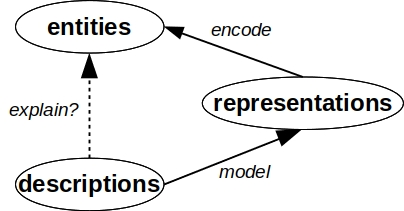
\includegraphics[scale=0.5]{representationProblem}
\caption{The Problem of Understanding.}
\end{figure}

In the discipline of Kolmogorov complexity, researchers solve the problem of representation by assuming that the set $\mathcal{E}$ is well defined, countable, and that there exists a total encoding function $f:\mathcal{E} \rightarrow \mathbb{N}$ from the set of entities to the set of natural numbers (a kind of Gödel numbering). In the theory of nescience we borrow this idea of encoding entities with numbers, or equivalently, strings of symbols. The main difference is that we address the problem of encoding an arbitrary set $\mathcal{E}$ by turning it around, that is, by defining a total function $\mathcal{O}_\mathcal{E}:\mathcal{S}^\ast \rightarrow \mathcal{E}$ from the well defined set $\mathcal{S}^\ast$ of all possible finite strings from an alphabet $\mathcal{S}$ to the, perhaps not countable and even not well defined, set $\mathcal{E}$ of entities under study.

Our function $\mathcal{O}_\mathcal{E}$, that depends on the set $\mathcal{E}$, is a kind of oracle (inspired by the concept of oracle Turing machine from Definition \ref{def:Oracle-Turing-Machine}) that is able to fully reconstruct an entity $\mathcal{O}_\mathcal{E} (x) \in \mathcal{E}$ given its encoding string $x \in \mathcal{S}^\ast$, without requiring additional information. Of course, this oracle is a conceptual idea that cannot be built in the real world for the majority of the sets $\mathcal{E}$, but assuming its existence will allow us to explain and prove important properties of how the process of scientific discovery works. $\mathcal{O}_\mathcal{E}$, being an oracle and not a regular function, is limited in terms of the mathematical operations in which it can used, as we will see below.

We assume that there exists a single, unique, physical world, that is independent of observers. We also assume that for some collections of entities $\mathcal{E}$ it is free of logical contradiction to assume the existence of an oracle $\mathcal{O}_\mathcal{E}$ (see the scientific representation problem in Section \ref{sec:scientific_representation}). Without any loss of generality, for the rest of this book we will only consider binary strings as encoding of entities.

\begin{definition}
\label{def:descriptions_topic}
Let $\mathcal{E}$ be a set of entities. A \emph{representation function} is an oracle $\mathcal{O}_\mathcal{E}:\mathcal{B}^\ast \rightarrow \mathcal{E}$ from the elements of the set $\mathcal{B}^\ast$ of all possible finite binary strings to the elements of the set $\mathcal{E}$ of entities under study.
\end{definition}

Only the elements of the set $\mathcal{B}^\ast$, that is, binary strings, can serve as representations of entities (problem of ontology). We do not allow drawings, or any other form of physical models, unless they are converted into binary strings. We do not make any distinction between a scientific representations and any other kind of representations (demarcation problem). It is up to the oracle to decide which entity is encoded by each representation. It is also important to note that the oracle $\mathcal{O}_\mathcal{E}$ is total, that is, all possible strings represent entities (no targetless models allowed).

\begin{example}
\label{ex:not_unique_oracle}
Given a set of entities $\mathcal{E}$, if a representation oracle $\mathcal{O}_\mathcal{E}$ exists, it is not unique. For example, a binary not oracle (transform the zeros of a binary string into ones and the ones into zeros) that assigns to each string $x \in \mathcal{B}^\ast$ the entity $\mathcal{O}_\mathcal{E} \left( \neg x \right)$ would be also a representation function.
\end{example}

We could have used an universal oracle machine instead of individual oracles. An universal oracle machine is a machine $\mathcal{U}_\mathcal{O}$ that given as input the encoding of an oracle $\mathcal{O}_\mathcal{E}$ and a string $s$, it computes $\mathcal{U}_\mathcal{O} \left( \langle \mathcal{O}_\mathcal{E}, s \rangle \right) = \mathcal{O}_\mathcal{E} \left( s \right)$. Universal machines make more sense when they are applied to the universal set $\xi$ that contains everything. However, that would make the the process of scientific discovery more difficult in practice. We prefer to work with a sets of entities $\mathcal{E}$ that correspond to particular areas of knowledge, and select one oracle $\mathcal{O}_\mathcal{E}$ for each set $\mathcal{E}$ (the best one according to our current knowledge).

\begin{example}
\label{ex:description_dna}
When the topics under study are animals we could start using as encodings a detailed description of the body of those animals. In this case, the oracle would be an hypothetical machine that given its description is able to reproduce the original animal. As we get a better understanding of the biology of life we can consider to use an alternative encoding based on the DNAs of the animals. Both encodings are valid representations of the entities.
\end{example}

We use an oracle function instead of an oracle relation $\mathcal{R}_\mathcal{O} \subset \mathcal{B}^\ast \times \mathcal{E}$, because our aim is not about matching strings with their correspoding entities, but building an entity given its representation. The capacity of the oracle of reconstruct the original entities is what justifies the fact that we can formulate hypotheses about entities given their representations (surrogative reasoning). According to the theory of nescience, scientific research would be not only about figuring out how to properly encode entities, but also about discovering the inner workings of the decoding oracles. 

The goal of encoding entities in the theory of nescience is different from that of Shannon's information theory, as Example \ref{ex:shannon_encoding} shows.

\begin{example}
\label{ex:shannon_encoding}
Consider a set $\mathcal{E}$ composed by two books, "The Ingenious Nobleman Sir Quixote of La Mancha" and "The Tragedy of Romeo and Juliet". We could encode the fist book with the string "0" and the second one with the string "1". Although those strings allow us to uniquely identify each book in the set, they are not proper encodings in the sense of the theory of nescience. Information theory is about how to uniquely identify an object given a reference and it requires that both, sender and received agree about a mapping between references and objects. Meanwhile, in the theory of nescience we are interested in how to provide a representation that captures all the details and nuances of the original objects. For example, given the strings "0" and "1" it is not possible to make any hypothesis about the influence of Cervantes in the work of Shakespeare.
\end{example}

An alternative way to deal with the problem described in Example \ref{ex:shannon_encoding}, where we used artificially short descriptions, would be to require the set $\mathcal{E}$ to be infinite, as Kolmogorov complexity does (we can not cheat an infinite number of times). However, even requiring the set of entities to be infinite, not every possible encoding schema can guarantee that the highly desirable property of surrogative reasoning is satisfied.

As it was shown in Example \ref{ex:not_unique_oracle} and Example \ref{ex:description_dna}, the entities of $\mathcal{E}$ might be encoded in multiple ways (problem of style). Different oracles will admit different encoding schemas. Some of those strings are better representations of an entity than others (standard of accuracy). Which representation is the best depends on the kind of questions we are interested to answer. In ant case, our aim should be to use those representations that make the size of the oracle (the amount of inner knowledge we assume the oracle contains) as small as possible.

Recall that the oracle is a total funcion, that is, all possible strings must represent an entity, including the incomplete ones. The more information is missing from a representation, the harder would be for us to understand how the oracle works. We must be careful with those representations that do not capture all the details about the original entities, since the results of our analyses could present some bias. In Chapter \ref{chap:Miscoding} we will study in detail the problem of errors due to the miscoding of abstract entities, and we will see that not only representations are about entities, but also we require that entities should be about representations (requirement of directionality).

\begin{example}
The data used in time of Ptolomeo about the position of celestial bodies along the year was a misencoding of the entity "position of celestial bodies". A better encoding was the data provided by Tycho Brahe. Today, we have even better encodings.
\end{example}

We distinguish between \emph{knowable} and \emph{unknowable} entities.

\begin{definition}
We say that an entity $e \in \mathcal{E}$ is \emph{knowable} if there exists at least one $r \in \mathcal{B}^\ast$ such that $\mathcal{O}_\mathcal{E}(r) = e$. An entity $e \in \mathcal{E}$ is \emph{unknowable} if it is not knowable.
\end{definition}

A priori, it is not possible to determine if a set of entities $\mathcal{E}$ is knowable, unknowable, or partially knowable. Selecting the right knowable entities to study is a matter of trial and error. In this book we have nothing to say about unknowable entities, beyond that the unknowability of an entity cannot be proved nor discovered.

\begin{definition}
Let $e \in \mathcal{E}$ a knowable entity. We call the \emph{set of representations} for $e$, denoted by $\mathcal{R}_e$, to $\{ r \in \mathcal{B}^\ast : \mathcal{O}_\mathcal{E} (e) = r \}$.
\end{definition}

In figure \ref{fig:entities_topics_1} we have a representation of an hypothetical oracle from the set of finite binary strings $\mathcal{B}^\ast$ to the set of entities $E$; we have also depicted a particular entity $e_1$, the subset of strings $\mathcal{R}_{e_1}$ that encode that entity, and a particular representation $r_1$. Since the set $\mathcal{E}$ is, in general, not well defined, the inverse function $\mathcal{O}_\mathcal{E}^{-1}(e_1)$ cannot be computed in practice.

\begin{figure}[h]
\centering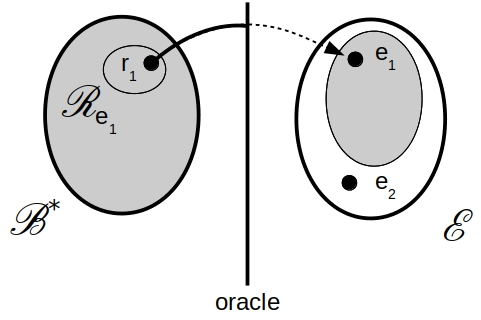
\includegraphics[scale=0.5]{entities_topics_1}
\caption{\label{fig:entities_topics_1}Encodings and Entities.}
\end{figure}

A consequence of working with finite strings as representations is that it might happen that there exist entities that are not encoded by any representation (see the gray areas in Figure \ref{fig:entities_topics_1}, in particular, the entity $e_2$ is not encoded by any representation). Intuitively, we could say that for some domains of knowledge the number of problems is much higher than the number of solutions.

\begin{example}
If the collection of entities under study are real numbers, it turns out that there exist numbers that can not be encoded using finite binary strings, since the set $\mathbb{R}$ has the cardinality of the continuum, and the set $\mathcal{B}^\ast$ is numerable.
\end{example}

Since our knowledge about the entities and the inner workings of the oracle are incomplete, in practice we will working with another set $\hat{\mathcal{R}}_e \subseteq \mathcal{B}^\ast$ of strings that we believe are close to the representations $\mathcal{R}_e$ that encode the entity $e$. The elements that belong to $\hat{\mathcal{R}}_e$ usually change over time, as we better understand the entities of $\mathcal{E}$, and how the oracle encode these entities as strings. The more abstract is our set of entities $\mathcal{E}$, the more difficult will be to approximate them as strings in $\hat{\mathcal{R}}_e$.

\begin{example}
\label{ex:luminiferous_ether}
The entity "luminiferous ether" was a theoretical postulate about a hypothetical medium in which the light would propagate. The ether was used as an explanation of how a wave-based light could propagate through the empty space. In 1887, the results of the Michelson-Morley experiment suggested that the ether did not exist, and after Einstein formulated his special theory of relativity, that successfully explained how light propagates through empty space, the idea of ether was completely dropped.
\end{example}

A consequence of working with approximations (the set $\hat{\mathcal{R}}_e$) instead of the true representations (the set $\mathcal{R}_e$) is that some of the candidate strings currently in use might encode a different entity from what we were expecting.

\begin{example}
\label{ex:polywater}
In 1961, the Soviet physicist Nikolai Fedyakin, performed a series of experiments resulting in what was seemingly a new form of water. The new water, called polywater, showed a higher boiling point, a lower freezing point, and much higher viscosity than ordinary water. Later experiment showed that polywater was nothing more than contaminated water with small amounts of impurities.
\end{example}

\begin{remark}
One of the problems of science, and in general of any human intellectual activity, is that people tend to confuse symbols with what they represent. The theory of nescience has been carefully designed to avoid this problem, by means of clearly stating the difference between research entities and the representation of entities. However, keeping this distinction always explicit in the explanations would make the book very difficult to read. We have tried to find a compromise between clarity in the exposition and rigor in the definitions. Sometimes, during the introduction of new ideas we talk in general about a \emph{topics}, meaning an entity, a representation, or both, an entity and its representation. But, in the mathematical definitions and propositions we always make this difference unequivocal. In case of doubt about what we mean, please take the mathematical definitions as the authoritative reference. 
\end{remark}

%
% Section: Joint Representations
%

\section{Joint Representations}
\label{sec:descriptions_joint_topic}

We have seen in the previous section that there exists more than one way to encode an entity $e \in \mathcal{E}$, what we have called the set $\mathcal{R}_e$ of representations of the entity. Some of these representations have a high quality, in the sense that they contain all the information required by the oracle to reconstruct (in whatever way the oracle manages to do that) the original entity. But also, in the set $\mathcal{R}_e$ there exists low quality representations, that is, representations that lack many of the details needed to fully reconstruct the entity. Furthermore, the set $\mathcal{R}_e$ can contain representations that include information that is wrong, symbols that the oracle will automatically ignore during the reconstruction, but that they will mislead us when understanding the entity. In Chapter \ref{chap:Miscoding} we will study how to measure the error due to incomplete and wrong representations, and in this section we will introduce a mechanism to improve our currently known representations.

If we want to increase our knowledge about an entity, we have to find the best possible representation for that entity, that is, a representation that is complete and correct. One way to do that is simply try different strings until we come up with a high quality representation. However, that method could require a lot of time and it is impractical. A more efficient approach would be to complement our current bad representation with more (potentially missing) symbols, or by combining those known representations that contain partial information. These two methods require the introduction of the concept of joint representation.

\begin{definition}
Let $s, t \in \mathcal{B}^\ast$ be two different representations. We call \emph{joint representation} of $s$ and $t$ to the concatenation string $st$.
\end{definition}

\begin{example}
\label{ex:lung_cancer}
Suppose that the research entity $e$ in which we are interested is the causes of lung cancer. In order to understand this entity, we have measured a collection of risk factors in a random sample of the population (smooking, exercise, diet, age, etc.). However, due to a problem with the sampling procedure, all the samples correspond to a subset of the population, for example, males. This dataset would be a representation $s$ for our entity $e$, but a very bad one, since it is strongly biased. If we have a second representation, corresponding the sample data of females $t$, the joint representation $st$ will be a better one that any of them, $s$ or $t$, isolated.
\end{example}

The concatenation of any two arbitrary representations is also a representation.

\begin{proposition}
Let $s, t \in \mathcal{B}^\ast$ be two different representations and $st$ its joint representation, then $st$ is also a representation.
\end{proposition}
\begin{proof}
As we have seen in Section \ref{sec:strings} the set $\mathcal{B}^\ast$ is closed under the operation of concatenation of strings, and the representation function $\mathcal{O}_\mathcal{E}$ is total.
\end{proof}

We do not require the set of representations $\mathcal{R}_e$ for a given entity $e \in \mathcal{E}$ to be closed under the operation of concatenation. That is, it might happen that $st \notin \mathcal{R}_e$, even if it is the case that $s \in \mathcal{R}_e$ and $t \in \mathcal{R}_e$.

The concept of joint representation is defined for every pair of strings $s, t \in \mathcal{B}^\ast$, even if they do not belong to the same set of representations $\mathcal{R}_e$, in other words, when $\mathcal{O}_\mathcal{E} \left( s \right) \neq \mathcal{O}_\mathcal{E} \left( t \right)$. This process of joining representations from different entities will be very usefull for the discovery of new research entities hitherto unknown (see Section \ref{sec:New_Research_Topics} and recall that all possible strings in $\mathcal{B}^\ast$ represent an entity).

The operation of string concatenation is associative, that is, $(rs)t = r(st)$, for all $r, s, t \in \mathcal{B}^\ast$. This property defines the algebraic structure of the sets of representations.

\begin{proposition}
The set $\mathcal{B}^\ast$ of representations together with the operation of concatenation has the structure of free monoid.
\end{proposition}
\begin{proof}
As we have seen in Section \ref{sec:strings} the operation of string concatenation in $\mathcal{B}^\ast$ is associative, and the empty string $\lambda$ plays the role of neutral element.
\end{proof}

We do no require the operation of joining representations to be conmutative with respect to the oracle function. Given the representations $s, t \in \mathcal{B}^\ast$ it might happen that the concatenation strings $st$ and $ts$ represent different entities, that is, $\mathcal{O}_\mathcal{E} \left( st \right) \neq \mathcal{O}_\mathcal{E} \left( ts \right)$.

The concept of joint representation can be extended to any arbitrary, but finite, collection of representations. In this way, we could add multiple partial representations to our research, or use them in the process of discovering new entities.

\begin{definition}
Let $r_1, r_2, \ldots, r_n \in \mathcal{B}^\ast$ be a finite collection of representations. We call \emph{joint representation} of $r_1, r_2, \ldots, r_n$ to the string $r_1 r_2 \ldots r_n$.
\end{definition}

It is easy to show that $r_1 r_2 \ldots r_n \in \mathcal{B}^\ast$ for all $r_1, r_2, \ldots, r_n \in \mathcal{B}^\ast$, that is, $\mathcal{B}^\ast$ is closed under the operation of concatenation of multiple, finite, representations.

%
% Section: Descriptions
%

\section{Descriptions}
\label{sec:descriptions_models}

So far, our aim with the strings of $\mathcal{B}^\ast$ has been to provide an enconding, or representation, as complete and detailed as possible of the entities of $\mathcal{E}$, no matter its length. However, as we have said in the preface of this book, human understanding requires the derivation of concise models for those entities, since human reasoning cannot be based on long representations.

\begin{example}
In Example \ref{ex:lung_cancer} we have shown that a good representation for the entity "lung cancer" could be a sample dataset in which we measure different risk factors. If smokers decide to quit smooking is not because they know and understand this large sample dataset, but because they know and understand the much simpler derived model "smooking increases the risk of lung cancer".
\end{example}

A description or model\footnote{In the theory of nescience use the words "description" and "model" interchangeably.} is a finite binary string mapped to a representation of an entity (recall Figure \ref{fig:entities_topics_models} from Chapter \ref{chap:Introduction}). Descriptions do not model entities (target systems) directly, they do so through string based representations. In the theory of nescience we require that descriptions must be computable, so we can fully and effectively reconstruct the original representations given their descriptions. The requirement of computability allows us to clearly state the limits of the concept of "description". For example, the problem of self-referential descriptions, like the Berry paradox\index{Berry paradox}, can be addressed in the scope of the limits of computation.

\begin{definition} [Model]
\label{def:descriptions_model}
Let $d \in \mathcal{B}^\ast$ be a binary string in the form $d = \langle TM,a \rangle$, where $TM$ is the encoding of a prefix free Turing machine and $a$ is the input string to that machine. If $TM(a)$ is defined, we say that $d$ is a \emph{description}\index{Description}. 
\end{definition}

Intuitively, a description is composed by two parts, a Turing machine that should compresses all the regularities found in this representation, and a string containing what is left, that is, the non-compressible part. Descriptions that do not compress representations are useless, as we will see below in this section.

\begin{definition}
\label{def:descriptions_model}
We define the \emph{set of descriptions}\index{Set of descriptions}, denoted by $\mathcal{D}$, as:
\[
\mathcal{D} = \{ d \in \mathcal{B}^\ast : d = \langle TM,a \rangle \wedge TM(a) \downarrow \}.
\]
Let $r \in \mathcal{B}^\ast$ be a representation. We define the set of \emph{descriptions for $r$}, denoted by $\mathcal{D}_r$, as:
\[
\mathcal{D}_r = \{ d \in \mathcal{D} : TM(a) = r \}.
\]
Finally, given an entity $e \in \mathcal{E}$, we define the set of \emph{descriptions for $e$}, denoted by $\mathcal{D}_e$, as:
\[
\mathcal{D}_e = \{ d \in \mathcal{D} : \exists r \in \mathcal{R}_e,\, TM(a) = r \}.
\]
\end{definition}

From an otological point of view, descriptions are just string based representations that satisfy the additional requirement of being computable. In this sense, descriptions are also representations, and so, there exists descriptions that describe descriptions. In practice it is not a good idea to use descriptions as the representation of entities, since what we are looking for in a good representation is that they contain as many details as possible about the original entities, not a concise encoding. Working with descriptions in the role of representations would make the job of scientific discovery very difficult for humans.

Since each description describes one, and only one, representation, we can define a function that maps descriptions into representations. Given that descriptions are Turing machines, it is natural to use as description function a universal Turing machine. Consequently, not only the individual descriptions of representations are computable, but also the function that maps descriptions into representations is also computable.

\begin{definition}
We call \emph{description function}\index{Description function}, denoted by $\delta$, to any universal Turing machine $\delta : \mathcal{D} \rightarrow \mathcal{B}^\ast$ that maps descriptions to their corresponding representations.
\end{definition}

If $d = \langle TM, a \rangle$ is a description of the representation $r$, then we have that $\delta \left( d \right) = \delta \left( \langle TM, a \rangle \right) = TM(a) = r$.

Inspired by the Occam's razor principle\index{Occam's razor principle}\footnote{The Occam's razor principle refers to the number of assumptions of an explanation, not to the length of the explanation itself.}, if two explanations are indifferent, we should prefer the shortest one. Therefore, the limit of what can be known (understand) about a representation, that is, its perfect model, is given by the shortest description that allows us to reconstruct this representation. Of course, what we know about the original entity is conditional to the quality of the representation.

\begin{definition}
\label{def:descriptions_perfect_model}
Given the set of descriptions $\mathcal{D}_r$ of a representaton $r \in \mathcal{B}^\ast$, let $d_r^{\star} \in \mathcal{D}_r$ be the shortest possible description of $r$ using the standard shortlex ordering. We call $d_r^{\star}$ the \emph{perfect description}\index{Perfect description} of the representation $r$.
\end{definition}

Unfortunately, the perfect description of a representation is in general not known and, as Proposition \ref{prop:nescience-kolmogorov} shows, there exist no algorithm to compute it. In practice what we have to do is to use an approximation to estimate how far our current best description is from the perfect one, that is, how much we do not know about a particular representation for an entity (see Chapter \ref{chap:Redundancy}).

\begin{proposition}
\label{prop:nescience-kolmogorov}
Given a representation $r \in \mathcal{B}^\ast$, we have that $l \left( d_r^{\star} \right) = K\left( r \right)$.
\end{proposition}
\begin{proof}
Apply Definition \ref{def:Kolmogorov-Complexity} and the fact that we require that the Turing machines $TM$ used in definitions $\langle TM,a\rangle$ must be prefix-free.
\end{proof}

The actual length of a description $l \left( d \right)$ for a representation $r$ is something that depends on the particular enconding of Turing machines used. The encoding method is given by the description function $\delta$ used. Fortunately, if we replace our description function by a different one, the length of perfect models do not change (up to an additive constant that does not depend on the representations themselves).

\begin{corollary}
Let $r \in \mathcal{B}^\ast$ be a representation, $\delta$ and $\dot{\delta}$ two different description functions, and $d_r^{\star}$ the perfect description of the representation $r$ using $\delta$ and $\dot{d}_r^{\star}$ the perfect description using $\dot{\delta}$, then we have that $l \left( d_r^{\star} \right) \leq l \left( \dot{d}_r^{\star} \right) + c$ where $c$ is a constant that does not depend on $r$.
\end{corollary}
\begin{proof}
Apply Theorem \ref{prop:nescience-kolmogorov} and Theorem \ref{def:Invariance-theorem}.
\end{proof}

In general, in the theory of nescience we are not interested in computing the actual value of the nescience about an entity given a description and a representation. Instead what we are interested is in the ordering of the different possible pairs of descriptions and representations given their nescience. In this sense, the details of the particular universal Turing machine used in practice are not relevant\footnote{Do not confuse the inner workings of the universal Turing machine that maps descriptions to representations, in which we are not interested, with the inner workings of the universal oracle Turing machine that maps representations to entities, in which we are interested, since this knowledge is critical to understand how things work.}. For the rest of this book we will assume that $\delta$ is fixed to a reference universal Turing machine. For example, in Section \ref{sub:ax_type_theory} we use as univeral Turing machine the lambda calculus. Alternatively, the reader could consider that all the theorems provided in this book that deal with the length of shortest models are valid up to an additive constant that does not depend on the topics themselves.

A remarkable consequence of Proposition \ref{prop:nescience-kolmogorov} is that perfect descriptions must be incompressible, that is, \emph{perfect knowledge implies randomness} (see Section \ref{sec:incompressibility_randomness}).

\begin{corollary}
Let $d_r^{\star}$ be the perfect description of a representation $r$, then we have that $K \left( d_r^{\star} \right) = l \left( d_r^{\star} \right)$.
\end{corollary}
\begin{proof}
Having $K \left( d_r^{\star} \right) < l \left( d_r^{\star} \right)$ would be a contradiction with the fact that $d_r^{\star}$ is the shortest possible description of $r$.
\end{proof}

The converse, in general, does not hold, since we could have a random description that it is not the shortest possible one, that is, a description $d$ for a reprsentation $r$ such that $l(d) = K(d)$ but $l(d_r^{\star}) < l(d)$.

\begin{example}
\label{ex:description_neural}
We could define a deep neural network\index{Neural network} with an input layer of one thousands nodes, ten hidden layers of fifty thousands nodes each, and an output layer of one thousand nodes, and then train the network to output a fixed string of one thousand 1's for any given input string. The Kolmogorov complexity of this neural network is much higher that the complexity of a string of one thousand 1's.
\end{example}

There is little value on a descriptions that is longer than the representation it describes.

\begin{definition}
\label{def:trivial_model}
Let $r \in \mathcal{B}^\ast$ be a representation, and $d \in \mathcal{D}_r$ one of its descriptions. If $l(d) \geq l(r)$, we say that $d$ is a \emph{pleonastic description}\index{Pleonastic description} of the representation $r$.
\end{definition}

\begin{example}
\label{ex:topics_models_graph}
Consider the set of all possible finite graphs\index{Graph}. Since graphs are abstract mathematical objects, we need a way to represent them as strings, for example, by using a binary encoding of their adjacency matrices (see Section \ref{sec:Graphs} for an introduction to graphs). The description $d = \langle TM, r \rangle$, where $r$ is the representation of a graph and $TM$ is a Turing machine that just halts, will be part of $\mathcal{D}_r$ since $TM(r) = r$. We are concerned about the fact that this description may not be shortest possible description of $r$.
\end{example}

It might happen that there is no shortest possible description of a representation than the representation itself. This is the case when representations are random, or incompressible, strings. And, as we have seen in Section \ref{sec:incompressibility_randomness} the overhelming majority of strings are incompressible. It is useless to do research about random representation, since it is not possible to find shorter models for that representation.

The concept of perfect description can be generalized from individual representations to entities. This generalization allow us to study the nature and properties of these entities.

\begin{definition}
\label{def:entities_perfect_model}
Given the set of descriptions $\mathcal{D}_e$ of an entity $e \in \mathcal{E}$, let $d_e^{\star} \in \mathcal{D}_e$ be the shortest possible description of $\mathcal{D}_e$ using the standard shortlex ordering. We call $d_e^{\star}$ the \emph{perfect model}\index{Perfect model} of entity $e$.
\end{definition}

For each possible representation $r$ of $e$ we can compute its perfect description $d_r^{\star}$. Then, the perfect description $d_e^{\star}$ for $e$ would be the shortest of this collection of perfect descriptions of the representations.

An interesting case is when all the descriptions that compose $\mathcal{D}_e$ are pleonastics, that is, there is no model that it is shorter than the representation for all the possible representations of the entity. That would the case if all the representations of the entity $e$ are random strings. In this particular case, scientific research would be doomed, since it is not possible to find a suitable model for $e$. The fact that we can understand and make predictions about $e$ will be limited by the length of the non-compressible representations of $e$.


%
% Section: Models for Joint Representations
%

\section{Descriptions for Joint Representations}
\label{sec:description_joint_represenation}

In Section \ref{sec:descriptions_joint_topic} we introduced the concept of joint representation $ts$ of two individual representations $t$ and $s$. In this section we are interested in to study how the length of the perfect description of a joint representation relates to the length of the perfect descriptions of the individual representations.

The length of the perfect description of a joint representation is greater or equal than the length of the perfect description of the individual representations. That is, the more information we include in a representation, the longer will take to describe it. 

\begin{proposition}
\label{prop:joint_length}
Let $t,s \in \mathcal{B}^\ast$ be two representations and $m_{t}^{\star}$, $m_{s}^{\star}$ and $m_{ts}^{\star}$ the perfect descriptions of the representatons $t$, $s$ and the joint representation $ts$ respectively. We have that $l \left( m_{ts}^{\star} \right) \geq l \left( m_{t}^{\star} \right)$ and $l \left( m_{ts}^{\star} \right) \geq l \left( m_{s}^{\star} \right)$.
\end{proposition}
\begin{proof}
The statement $l \left( m_{ts}^{\star} \right) \geq l \left( m_{t}^{\star} \right)$ is equivalent to $K(ts) \geq K(t)$. Then apply Proposition \ref{prop:excess_kolmogorov}.
\end{proof}

Intuitively, adding more information to a representation is a good thing if this information is relevant to describe the entity in which we are interested. But adding non-relevant information will make our model unnecessarily long. Recall that the process of joining representations can be used to concatenate two partial representations of the same entity, or to extend a representation with additional missing symbols.

If the selected representations partially overlap, we could take advantage of this redundancy to come up with a shorter join description than simply joining the individual descriptions. In the worst case, the perfect description of a joint representation would be the concatenation of the perfect descriptions of the individual representations.

\begin{proposition}
\label{prop:joint_sum}
Let $t,s \in \mathcal{B}^\ast$ be two representations and $m_{t}^{\star}$, $m_{s}^{\star}$ and $m_{ts}^{\star}$ the perfect descriptions of the representatons $t$, $s$ and the joint representation $ts$ respectively. We have that $l \left( m_{ts}^{\star} \right) \leq l \left( m_{t}^{\star} \right) + l \left( m_{s}^{\star} \right)$.
\end{proposition}
\begin{proof}
The statement $l \left( m_{ts}^{\star} \right) \leq l \left( m_{t}^{\star} \right) + l \left( m_{s}^{\star} \right)$ is equivalent to $K(ts) \leq K(t) + K(s)$, then apply Proposition \ref{prop:additive_kolmogorov}.
\end{proof}

An interpretation of Proposition \ref{prop:joint_sum} is that including redundant information in the representation of an entity is not a problem from the point of view of finding its shortest possible description. In practice, we have to use that representation that makes the process of scientific discovery (finding the best model) as easy as possible, even if this representation is unnecessarily long. In contrast, Proposition \ref{prop:joint_length} claims that adding non-relevant symbols to a representation is something that has to be avoided.

Finally, next proposition proves that the order of the representations in the perfect description of a joint representation does not change its length.

\begin{proposition}
\label{prop:joint_order}
Let $t,s \in \mathcal{B}^\ast$ be two representations and $m_{ts}^{\star}$ and $m_{st}^{\star}$ the perfect descriptions of the joint representations $ts$ and $st$ respectively. We have that that $l \left( m_{ts}^{\star} \right) = l \left( m_{st}^{\star} \right)$.
\end{proposition}
\begin{proof}
The statement $l \left( m_{ts}^{\star} \right) = l \left( m_{st}^{\star} \right)$ is equivalent to $K(ts) = K(st)$, then apply Proposition \ref{prop:kolmogorov_order}.
\end{proof}

Since joining representations is not a conmutative operation, there is no way to guarantee that the strins $ts$ and $st$ encode the same entity. Note also that given the concatenated $ts$ we cannot infer the original $t$ and $s$, since they are not self-delimited strings.

Propositions \ref{prop:joint_length}, \ref{prop:joint_sum} and \ref{prop:joint_order} can be generalized to any arbitrary, but finite, collection of representations $t_1, t_2, \ldots, t_n$.

\begin{proposition}
\label{prop:joint_multiple_topics}
Let $t_1, t_2, \ldots, t_n \in \mathcal{B}^\ast$ be a finite collection of representations. Then, we have that:

\renewcommand{\theenumi}{\roman{enumi}}
\begin{enumerate}
\item $l(m_{t_1 t_2 \ldots t_n}^\star) \geq l(m_ {t_i}^\star) \; \forall \, 0 \leq i \leq n$,
\item $l(m_{t_1 t_2 \ldots t_n}^\star) \leq l(m_ {t_1}^\star) + l(m_ {t_2}^\star) + \ldots + l(m_ {t_n}^\star)$,
\item $l(m_{t_1 \ldots t_i \ldots t_j \ldots t_n}^\star) = l(m_{t_1 \ldots t_j \ldots t_i \ldots t_n}^\star) + c \; \forall \, 0 \leq i \leq j \leq n$,
\item $l(m_{t_1 \ldots t_{n-1}}^\star) \leq l(m_{t_1 \ldots t_{n-1} t_n}^\star)$.
\end{enumerate}
\end{proposition}
\begin{proof}
Apply Propositions \ref{prop:joint_length}, \ref{prop:joint_sum} and \ref{prop:joint_order} to individual pairs of topics $i$ and $j$.
\end{proof}

%
% Section: Conditional Descriptions
%

\section{Conditional Descriptions}

It is usually cumbersome to include all the information needed to reconstruct an entity in its description, since that would require very large strings for the majority of the entities. It is more convenient to assume some already existing background knowledge, and compute how much we do not know about an entity given that background. In this section we are going to study the concept of \emph{conditional descriptions}, that is, computing a description given another description. Conditional descriptions also play a very important role in the discovery of new knowledge: if by conditioning a description to some prior knowledge we reduce significantly the inaccuracy of a model, that would mean this prior knowledge is relevant to understand the entity.

\begin{definition}
Let $r, d, s \in \mathcal{B}^\ast$ be strings. We say that the string $\langle d, s \rangle$ is a \emph{valid conditional description}\index{Conditional model} of the representation $r$ given the string $s$, denoted by $d_{r \mid s}$, if $d = \langle TM, a \rangle$ is a description, and $TM \left(\langle a, s \rangle \right) = r$.
\end{definition}

The conditional description $d_{r \mid s}$ is based on two strings $a$ and $s$, that play very different roles. The string $a$ is the input to the Turing machine $TM$,  and it should contain the non-compresible part of the representation $r$. The string $s$ should be the description, or representation, of another entity whose knowledge can helps to understand the entity in which we are interested. For example, as we will see in Chapter \ref{chap:Redundancy}, the string $s$ is not taken into account when computing the surfeit of a conditional description.

Note that the conditional description $d_{r \mid s}$ does not belong to the set of valid description $\mathcal{D}$ for the representation $r$, since $s$ is required to compute the representation $r$, but it is not part of the description itself. A new definition is required to capture this new concept.

\begin{definition}
Let $r \in \mathcal{B}^\ast$ be a representation and $s \in \mathcal{B}^\ast$ an arbitrary string, we define the \emph{set of conditional descriptions}\index{Set of conditional descriptions} of $r$ given $s$, denoted by $\mathcal{D}_{r \mid s}$, as:
\[
\mathcal{D}_{r \mid s} = \{ d \in \mathcal{B}^\ast, d = \langle TM, a \rangle : TM \left(\langle a, s \rangle \right) = r \}.
\]
\end{definition}

For each representation $r \in \mathcal{B}^\ast$ there always exists a conditional description $d_{r \mid s}$ that describes $r$, as next proposition shows.

\begin{proposition}
\label{prop:description_implies_conditional}
Let $r \in \mathcal{B}^\ast$ be a representation and $s \in \mathcal{B}^\ast$ an arbitrary string. If $d \in \mathcal{D}_{r}$ then $d \in \mathcal{D}_{r \mid s}$.
\end{proposition}
\begin{proof}
We can use a conditional description $\langle \langle TM, a \rangle, s \rangle$ based on a Turing $TM$ machine that given the input $\langle a, s \rangle$ safely ignores the $s$ string.
\end{proof}

The converse of Proposition \ref{prop:description_implies_conditional} is not true. The fact that $d$ is a conditional description ($d \in \mathcal{D}_{r \mid s}$) does not implies that $d$ is also a description ($d \in \mathcal{D}_{r})$. We require that $TM \left(\langle a, s \rangle \right) = r$ but $TM \left( a \right) = r$ is not required, and it might not be the case.

We are interested in the concept of perfect conditional description. The perfect conditional description of a representation given a prior knowledge is the shortest possible string that allow us to fully reconstruct the representation assuming this prior knowledge.

\begin{definition}
Let $r \in \mathcal{B}^\ast$ be a representation, and let $d^\star_{r \mid s}$ be the shortest possible description of $r$ given the string $s$. We call $d^\star_{r \mid s}$ the \emph{perfect conditional description} of the representation $r$ given the string $s$, or perfect conditional description of $r$ given $s$ for short.
\end{definition}

Note that $d^\star_{r \mid s}$ is a perfect description of the representation $r$ conditional to the string $s$. That is, it might happen that the string $s$ is not a perfect description itself, or it is a representation that contains non-relevant symbols. In that case, we would have reached a perfect knowledge with respect to the $d$ part, but not for the $s$ part, of the combined $\langle d, s \rangle$ string.

The length of perfect conditional description is equal or shorter that their unconditional counterparts. That is, assuming some already existing background knowledge could reduce the effort required to describe a representation.

\begin{proposition}
\label{prop:description_conditional_inequality}
Let $r \in \mathcal{B}^\ast$ be a representation and $s \in \mathcal{B}^\ast$ an arbitrary string. We have that $l \left( d^\star_{r \mid s} \right) \leq l \left( d^\star_r \right)$.
\end{proposition}
\begin{proof}
The statement $l \left( d^\star_{r \mid s} \right) \leq l \left( d^\star_r \right)$ is equivalent to $K(r \mid s) \leq K(r)$, then apply Proposition \ref{prop:kolmogorov_conditional}.
\end{proof}

Next proposition shows the relation between the lengths of descriptions, join descriptions and conditional descriptions.

\begin{proposition}
\label{prop:description_conditional_joint}
Let $r, s \in \mathcal{B}^\ast$ two different representations. We have that:
\[
l \left( d^\star_{r \mid s} \right) \leq l \left( d^\star_r \right) \leq l \left( d^\star_{rs} \right)
\]
\end{proposition}
\begin{proof}
The statement $l \left( d^\star_{r \mid s} \right) \leq l \left( d^\star_r \right) \leq l \left( d^\star_{rs} \right)$ is equivalent to $K(r | s ) \leq K(r)$ and $K(r) \leq K(rs)$, then apply Proposition \ref{prop:kolmogorov_relations}.
\end{proof}

As it was the case of joint descriptions, the concept of conditional description can be extended to finite collections of representations.

\begin{definition}
Let $r, d, s_1, s_2, \ldots, s_n \in \mathcal{B}^\ast$ be strings. We say that the string $\langle d, s_1, s_2, \ldots, s_n \rangle$ is a \emph{valid conditional description}\index{Conditional model} of the representation $r$ given the strings $s_1, s_2, \ldots, s_n$, denoted by $d \mid s_1, s_2, \ldots, s_n$, if $d = \langle TM, a \rangle$ is a description, and $TM \left(\langle a, s_1, s_2, \ldots, s_n \rangle \right) = r$.
\end{definition}

In the next definition we provide the generalization of the concept of perfect conditional descriptions.

\begin{definition}
Let $r \in \mathcal{B}^\ast$ be a representation, and let $d^\star_{r \mid s_1, s_2, \ldots, s_n}$ be the shortest possible description of $r$ given the strings $s_1, s_2, \ldots, s_n$. We call $d^\star_{r \mid s_1, s_2, \ldots, s_n}$ the \emph{perfect conditional description} of the representation $r$ given the string $s_1, s_2, \ldots, s_n$, or perfect conditional description of $r$ given $s_1, s_2, \ldots, s_n$ for short.
\end{definition}

Next proposition generalizes Propositions \ref{prop:description_conditional_inequality} and \ref{prop:description_conditional_joint} to any arbitrary, but finite, collection of strings $s_1, s_2, \ldots, s_n$. Moreover, the proposition shows that the more background knowledge we assume for a representation, the shorter is the perfect description for that representation.

\begin{proposition}
Let $r, s_1, s_2, \ldots, s_n \in \mathcal{B}^\ast$ be a finite collection of strings. Then, we have that:
\[
l \left( d^\star_{r \mid s_1, s_2, \ldots, s_n} \right) \leq l \left( d^\star_r \right) \leq l \left( d^\star_{r,s_1, s_2, \ldots, s_n} \right)
\]
\end{proposition}
\begin{proof}
Apply Propositions \ref{prop:description_conditional_inequality} and \ref{prop:description_conditional_joint} to individual pairs of representations $i$ and $j$.
\end{proof}

The following proposition generalizes the idea that assuming more background knowledge to a description cannot increase its length.

\begin{proposition}
Let $r, s_1, s_2, \ldots, s_n, s_{n+1} \in \mathcal{B}^\ast$ be a finite collection of strings. Then, we have that:
\[
l \left( d^\star_{r \mid s_1, s_2, \ldots, s_n, s_{n+1}} \right) \leq l \left( d^\star_{r \mid s_1, s_2, \ldots, s_n} \right)
\]
\end{proposition}
\begin{proof}
Apply Propositions \ref{prop:description_conditional_inequality} and \ref{prop:description_conditional_joint} to individual pairs of representations $i$ and $j$.
\end{proof}

%
% Section: Areas
%

\section{Research Areas}
\label{sec:areas}

Entities can be grouped into research areas. The concept of area is useful as long as all the entities included in the area are related to a common knolewdge subdomain, or share a common property. The particular details of the grouping criteria depend on the practical applications in which the theory of nescience is being used.

\begin{definition}
Given a set of entities $\mathcal{E}$, we define a \emph{research area}\index{Research area} $\mathcal{A}$ as a subset of entities $\mathcal{A} \subset \mathcal{E}$.
\end{definition}

If we want to know how much we do not know about a research area, first we have to provide a representation for that area. In general areas are infinite, but the number of known representations is finite, and so, we can only describe the areas with respect to our current knowledge.

\begin{definition}
Let $\mathcal{A} \subset \mathcal{E}$ be an area. We define the \emph{known subset of the area}\index{Known subset of an area} $\mathcal{A}$, denoted by $\hat{\mathcal{A}}$, as the set composed by those entities $e_1, e_2, \ldots, e_n \in A$ for which at least one non-pleonastic description is known.
\end{definition}

We have to distinguish between the knowable subset of $\mathcal{A}$, composed by those entities for which there exists a representation, and the know subset of $\mathcal{A}$, composed by those entities for which we know a non-pleonastic description, that is, those entities for which somebody has already done some research about them. Of course, the set of known entities is a subset of the set of knowable entities.

As our understanding of a research area changes, the number of entities included in its known subset changes as well. The properties of areas studied in this book will be always relative to our current knowledge.

\begin{definition}
Let $\mathcal{A} \subset \mathcal{E}$ be an area with known subset $\hat{\mathcal{A}} = \{ e_1, e_2, \ldots, e_n \}$, and let  $R = \{ r_1, r_2, \ldots, r_n \}$ a set of representations, such that $r_i \in \mathcal{R}_{e_i}$. We call $R_{\hat{\mathcal{A}}}$ a \emph{representation of the area $\mathcal{A}$} given the known subset $\hat{\mathcal{A}}$, abbreviated as \emph{representation of $A$}.
\end{definition}

In the same way, we can introduce the concept of description of an area.

\begin{definition}
Let $R_{\hat{\mathcal{A}}} = \{ r_1, r_2, \ldots, r_n \}$ be the representation of an area $\mathcal{A}$. We call a \emph{description of the area $\mathcal{A}$} given the known subset $\hat{\mathcal{A}}$, abbreviated as \emph{description of $\mathcal{A}$}, and denoted by $d_{\hat{\mathcal{A}}}$, to any string in the form $\langle TM, a\rangle$ such that $TM(a) = \langle r_1, r_2, \ldots, r_n\rangle$.
\end{definition}

We can also define the set of descriptions of an area.

\begin{definition}
Let $R_{\hat{\mathcal{A}}} = \{ r_1, r_2, \ldots, r_n \}$ be the representation of an area $\mathcal{A}$. We define the set of \emph{descriptions for $R_{\hat{\mathcal{A}}}$}, denoted by $\mathcal{D}_{R_{\hat{\mathcal{A}}}}$, as:
\[
\mathcal{D}_{R_{\hat{\mathcal{A}}}} = \{ d \in \mathcal{D} : TM(a) = \langle r_1, r_2, \ldots, r_n\rangle \}.
\]
\end{definition}

Finally, we are interested in the perfect model for a research area, that is, the shortest possible string that fully describes its known subset. According to Definition \ref{def:trivial_model}, if we are aware of the existence of a entity $e \in A$, that entity should be part of $\hat{A}$, even in the case we have not started yet to do research about that particular topic.

\begin{definition}
Let $A \subset \mathcal{E}$ be an area with known subset $\hat{A}$, and let $d_{\hat{A}}^{\star} \in \mathcal{M}_{\hat{A}}$ be the shortest possible description of $A$. We call  $d_{\hat{A}}^{\star}$ the \emph{perfect description of the area $A$} given the known subset $\hat{A}$\index{Perfect description of an area}, abbreviated as \emph{perfect description of $A$}.
\end{definition}

Next proposition shows the relation between the description of an area, and the descriptions of the entities that compose the known subset of that area. In general, the models for an area are different from the collection of models of the individual topics.

\begin{proposition}
Let $A \subset \mathcal{E}$ be an area with known subset $\hat{A} = \{e_1, e_2, \ldots, e_n\}$, then we have that $l \left( d_{\hat{A}}^{\star} \right) \leq l(d_ {e_1}^\star) + l(d_ {e_2}^\star) + \ldots + l(d_ {e_n}^\star)$.
\end{proposition}
\begin{proof}
Apply Proposition \ref{prop:joint_multiple_topics}-ii. 
\end{proof}

Also, as it was proved in Proposition \ref{prop:joint_multiple_topics}, the order in which the representations are listed in the description of an area is not relevant when dealing with the perfect model for that area.

Areas can overlap, that is, given two areas $A$ and $B$ it might happen that $A \cap B \neq \varnothing$. Moreover, areas can be subsets of other areas, creating an hierarchy of areas. We are interested in the length of perfect models of areas in relation to the length of perfect models of other areas.

\begin{proposition}
Let $A, B \subset \mathcal{E}$ be two areas such that $A \subset B$, and let $\hat{A}$ and $\hat{B}$ be their know subsets respectively, then we have that $l \left( d_{\hat{A}}^{\star} \right) \leq l \left( d_{\hat{B}}^{\star} \right)$.
\end{proposition}
\begin{proof}
{\color{red} TODO}
\end{proof}

Next proposition \label{prop:areas_union} shows how the length of the shortest possible description of areas relate to the union and intersection of such areas.

\begin{proposition}
\label{prop:areas_union}
Let $A, B \subset \mathcal{E}$ be two areas with know subsets $\hat{A}$ and $\hat{B}$ respectively, then we have that $l \left( d_{\hat{A} \cup \hat{B}}^{\star} \right) = l \left( d_{\hat{A}}^{\star} \right) + l \left( d_{\hat{B}}^{\star} \right) - l \left( d_{\hat{A} \cap \hat{B}}^{\star} \right)$.
\end{proposition}
\begin{proof}
{\color{red} TODO}
\end{proof}

A consequence of Proposition \label{prop:areas_union} is that $l \left( d_{\hat{A} \cup \hat{B}}^{\star} \right) \leq l \left( d_{\hat{A}}^{\star} \right) + l \left( d_{\hat{B}}^{\star} \right)$, that is, when we combines two different research areas, how much we do not know about these areas decreases.

In the same way we introduced a chain rule for entropy in Proposition \ref{prop:chain_rule_entropy}, we can provide a chain rule for the shortest length for a description of a research area.

\begin{proposition}
Let $A, B \subset \mathcal{E}$ be two areas with know subsets $\hat{A}$ and $\hat{B}$, then we have that $l \left( d_{\hat{A} \cup \hat{B}}^{\star} \right) = l \left( d_{\hat{A}}^{\star} \right) + l \left( d_{\hat{B} \backslash \hat{A}}^{\star} \right)$.
\end{proposition}
\begin{proof}
{\color{red} TODO}
\end{proof}

%
% Section: References
%

\section{References}

{\color{red} TODO: Review this section.}

For more information about Russell's paradox, Cantor theorem and universal sets refer, for example, to \cite{jech2013set}. The idea of using a function to assigns to each symbol and well-formed formula of some formal language a unique natural number (Gödel number) was introduced by Kurt Gödel for the proof of his incompleteness theorems \cite{godel1931formal}. A detailed description of the Berry paradox from the point of view of computability can be found at \cite{chaitin1995berry}. For a detailed account of the implications of Kolmogorov complexity being true up to a constant, please refer to \cite{li2013introduction}. That oracle machines are not mechanical was stated by Turing when he introduced the concept of oracle machine in \cite{turing1939systems}.

\begin{itemize}
\item Intro to ontology: the things we can know about
\item Intro to epistemology: the problem of representation
\item What it is a representtaion: reference to oxford philosophy article
\item Reference to the concept of what it is research topic
\item The problem of representation in Kolmogorov complexity
\item Godel numbering
\item single, unique, physical world -> what it is thing called
\item Cantor theorem
\item Rusell paradox
\item Oracle Turing machine
\item ptolomeo and tycho
\end{itemize}

\emph{universal oracle machine}

Should be require the oracles to be minimal?

%
% CHAPTER: Miscoding
%

%
% CHAPTER: Miscoding
%

\chapterimage{Escher.pdf} % Chapter heading image

\chapter{Miscoding}
\label{chap:Miscoding}

\begin{quote}
\begin{flushright}
\emph{Some mathematical statements are true for no reason,\\
they're true by accident.}\\
Gregory Chaitin
\end{flushright}
\end{quote}
\bigskip

For the majority of the scientific disciplines, the set $\mathcal{E}$ of entities under consideration will be composed by abstract elements, or other kind of objects, that cannot be directly studied. If we want to understand them we have to use an indirect method. As we have seen in the previous chapter, the approach proposed by the theory of nescience is to work with representations (i.e. strings of symbols) instead of using the original entities; what we call the set $\mathcal{R}$ of representations. Unfortunately, proceeding in this way introduce new problems: since we do not fully understand the elements of $\mathcal{E}$, otherwise we will not be doing research, the representations used probably will not be as complete and accurate as they should. This limitation has serious implications, since an error in the representation of an entity will induce an error in the model we use to describe that entity. It is of utmost importance to characterize this type error, and to understand its implications.

{\color{red} TODO: say more ...}

Miscoding is a quantity that measures the error due to bad encodings. We propose a definition of miscoding based on the length of the shortest computer program that can print a correct representation given an incorrect one. Intuitively, miscoding quantifies the effort (measured as the length of a program) required to fix the incorrect representation.

{\color{red} TODO: say more ...}

In general, the ideal representations of the entities are not known, and so, we cannot compute how far our current representations are from those strings. From a theoretical point of view we could take advantage of the oracle machine used to characterize the set $\mathcal{E}$, since that (abstract) machine knows the answer. Unfortunately, there exists some limitations with respect to the kind of questions we can ask to the oracle that have to be taken into account.

In this chapter we will formally introduce the concept of miscoding and study its properties. We will also see how miscoding behaves when dealing with joint representations, and how to compute the miscoding of categories and research areas.

%
% Section: Miscoding
%
\section{Miscoding}
\label{sec:miscoding}

Miscoding refers to the fact that our current representation of the entity $e \in \mathcal{E}$ might not be the right one, that is, instead of working with a string $r_e \in \mathcal{R}_e$ that perfectly encodes $e$, it might happen we are studying another string $r \in \mathcal{R}_e$ that it is, hopefully, close to $r_e$ but not necessarily equal. We are interested in to compute the distance between the string $r$ and the perfect one $r_e$ as a quantitative measure of the error we are introducing with a wrong encoding of the entity $e$. Unfortunately, we do not know $r_e$, since, in general, it does not exists a computable function from $\mathcal{R}$ to $\mathcal{E}$. Recall that the only thing we have to our disposal is an abstract oracle machine $f_\mathcal{E}$ that knows which strings represents each entity (see Section \ref{sec:representations}).

We start by distinguishing between valid representations, that is strings that contain all the information required by the oracle to reconstruct an entity, and non-valid representations.

\begin{definition}
Let $\mathcal{E}$ be a collection of entities, and $f_\mathcal{E}$ and encoding function. We define the set of valid representations for $\mathcal{E}$, denoted by $\mathcal{R}_\mathcal{E}$, as the domain of $f_\mathcal{E}$.
\end{definition}

We can safely assume (it is free from logical contradictions) that the oracle machine also knows how far is $r$ from $r_e$, for all $r \in \mathcal{R}$ and all $r_e \in \mathcal{R}_\mathcal{E}$. Unfortunately, if we ask the oracle how far is a particular $r$ from perfectly encoding the entity in which we are interested, the oracle will require from us to specify the entity in which we are interested. And the only way to tell the oracle which one is that entity is by means of using $r_e$, which, of course, we do not know. The work around we propose to solve this problem is to ask to the oracle how far is $r$ from encoding \emph{any} entity from $\mathcal{E}$.

\begin{definition} [Miscoding]
\label{def:miscoding}
Let $r \in \mathcal{R}$ be a representation. We define the \emph{miscoding} of $r$, denoted by $\mu(r)$, as:
\[
\mu(r) = \overset{o}{ \underset{s \in \mathcal{R}_\mathcal{E}} \min} \frac{ \max\{ K(r \mid s), K(s \mid r) \} } { \max\{ K(r), K(s) \} }
\]
\end{definition}

Where the quantity $\overset{o}{ \underset{s \in \mathcal{R}_\mathcal{E}} \min}$ has to be computed by the oracle. Intuitively, the more ignorant we are about an entity, the bigger will be the miscoding of our current representation, since a better understanding of that entity means that we should be able to provide an encoding closer to a perfect one.

Miscoding is computed using a two-way approach: we require the oracle to compute the length of the shortest computer program that can print the string $s$ encoding the closest possible entity given our representation $r$, and the other way around, that is, to compute the length of the shortest computer program that can print $r$ given the string $s$. That is, a perfect representation has to include all the information required to reconstruct an entity, but no more. Miscoding is about including only relevant symbols, meanwhile surfeit (see Chapter \ref{chap:Redundancy}) is about including only those symbols that are needed.

In our definition of miscoding we have used a relative measure, instead of the absolute one, because besides to compare the miscoding of different encodings for the same entity, we are also interested in comparing the miscoding of different entities.

The miscoding of a representation $r$ is always a number between $0$ and $1$.

\begin{proposition}
\label{prop:range_miscoding}
We have that $0 \leq \mu(r) \leq 1$ for all $r \in \mathcal{R}$.
\end{proposition}
\begin{proof}
Given that $0 \leq \frac{ \max\{ K(s \mid t), K(t \mid s) \} } { \max\{ K(s), K(t) \} } \leq 1$ for all $t \in \mathcal{T}$ and all $s \in \mathcal{T}_\mathcal{E}$, since $\mathcal{T}_\mathcal{E} \subseteq \mathcal{T}$ and Proposition {\color{red} XX}.
\end{proof}

Miscoding is equal to zero if, and only if, the representation $r$ is one of the possible valid representation of an entity $e$.

\begin{proposition}\label{prop:perfect_encoding}
Let $t \in \mathcal{T}$ a topic, we have that $\mu(t) = 0$ if, and only if, $t \in \mathcal{T}_\mathcal{E}$.
\end{proposition}
\begin{proof}
Let $t \in \mathcal{T}_\mathcal{E}$, then by Proposition {\color{red} XX} we have that $K(t \mid t) = 0$ and so, $\mu(t) = 0$. In the same way, let's assume that $\mu(t) = 0$, then there exists at least one $s \in \mathcal{T}_\mathcal{E}$ such that $\frac{ \max\{ K(s \mid t), K(t \mid s) \} } { \max\{ K(s), K(t) \} } = 0$, and given Proposition {\color{red} XX} we have that $t = s$.
\end{proof}

According to Proposition \ref{prop:perfect_encoding}, if the miscoding of $t$ is equal to 0 we can conclude that $t$ perfectly encodes an entity $e$. The problem is that there is no way to know which one is the entity encoded by $t$. Of course, given our scientific intuition, we could guess the entity encoded, but from a mathematical point of view, we can not prove we are right. Moreover, with time and more research, it might happen that we change our mind about the nature of the encoded entity $e$ (see Example \ref{ex:phlogiston}).

An entity $e \in \mathcal{E}$ can have multiple representations, given by the set $\mathcal{R}_e$. Fortunately, miscoding is a quantity that does not depend on the representation selected (see the problem of style in Section \ref{sec:scientific_representation}).

\begin{proposition}
Let $t \in \mathcal{R}$ be a representation with $\mu(t) = \mu_t$, then we have that
\[
\mu_t \leq \frac{ \max\{ K(s \mid t), K(t \mid s) \} } { \max\{ K(s), K(t) \} } \quad \textrm{for all} \quad s \in \mathcal{T}_\mathcal{E}
\]
\end{proposition}
\begin{proof}
The existence of an $s \in \mathcal{R}_\mathcal{E}$ such that $\frac{ \max\{ K(s \mid t), K(t \mid s) \} } { \max\{ K(s), K(t) \} } < \mu_t$ is a contradiction with the fact that $\mu_t$ is the minimum reached for all possibles $s \in \mathcal{T}_\mathcal{E}$.
\end{proof}

Given an entity $e$, we have seen that all the representations that belong to $\mathcal{R}_e$ are equally good form the point of view of miscoding, since all of them have a miscoding of $0$. The question is which one we should use in our research? From a practical point of view, we should select that representation that makes it easier to gather new knowledge about the original entity, that is, to reduce the inaccuracy and surfeit of candidate models (see Section {\color{red} XX}).

\begin{example}
Assume we have a time series $ts$ composed $m$ measurements $x_1, \ldots, x_m$ collected at fixed time intervals from a physical phenomena with a sinusoidal behavior, and assume we have trained a neural network $nn$ that perfectly fits the data, that is, given a time $t$ as input it returns $x_t$. Both representations have the same miscoding, that is $\mu(ts) = \mu(nn)$. An analysis of the cycles of the time series will allow us to discover that the best model for this particular physical phenomena seem to be a sine function, however, no currently known machine learning approach will arrive at the same conclusion having as input the architecture of the neural network (number of layers, sizes, and trained weights). Of course, the oracle is so smart that, in fact, it did it.
\end{example}

%
% Section: Reducing Miscoding
%
\section{Reducing Miscoding}

As we have seen in Section \ref{sec:descriptions_joint_topic}, a possible way to imporove the quality of our current representations, is by adding, or removing, symbols from our current representation.

\begin{theorem}
Let $r \in \mathcal{R}$ be a representation such that $\mu(r) >0$, then at least one of the following cases is true:
\begin{enumerate}[label=(\roman*)]
\item there exist a $s \in \Sigma^{+}$ such that $r \oplus s <_N s$ or $s \oplus r <_N s$,
\item there exists a $t \in \Sigma^{+}$ in the form $r = \alpha \oplus t \oplus \beta$ with $\alpha, \beta \in \Sigma^\ast$ such that $t <_N r$.
\end{enumerate}
\end{theorem}
\begin{proof}
{\color{red} TODO}
\end{proof}


%
% Section: Joint Miscoding
%
\section{Joint Miscoding}
\label{sec:joint_miscoding}


{\color{red} TODO: Extend}

A similar approach could be used to discover new unknown entities, by means of combining the (possible approximate) representations of the already known entities.

In both cases, we require the concatenation of strings. In this section we study how the concept of miscoding behaves when we concatenate two representations.

\begin{definition}
Let $r, s \in \mathcal{R}$ two different representations. We define the \emph{joint miscoding} of the representations $r$ and $s$, denoted by $\mu(r, s)$, as:
\[
\mu(r, s) =  \overset{o}{ \underset{t_e \in \mathcal{T}_\mathcal{E}} \min} \frac{ \max\{ K(t_e \mid ts), K(ts \mid t_e) \} } { \max\{ K(t_e), K(ts) \} }
\]
\end{definition}

Explain ...

\begin{example}
{\color{red} PENDING}
\end{example}

$\mu(r, s) = \mu(rs)$

The joint miscoding of two representations is always a number between $0$ and $1$. This allow us to compare the joint miscoding of unrelated entities.

\begin{proposition}
We have that $0 \leq \mu(t,s) \leq 1$ for all $t, s \in \mathcal{T}$.
\end{proposition}
\begin{proof}
Given Definition \ref{def:descriptions_extended_topics} apply Proposition \ref{prop:range_miscoding}.
\end{proof}

When dealing with the concept of joint miscoding, the order in which the representations are listed is not relevant.

\begin{proposition}
We have that $\mu(t,s) = \mu(s,t)$ for all $t,s \in \mathcal{T}$.
\end{proposition}
\begin{proof}
{\color{red}: Apply Propositions \ref{prop:kolmogorov_order} and \ref{prop:joint_order}.}
\end{proof}

This is not true ...

The joint miscoding of two representations is greater or equal than the miscoding of any of them isolated. Intuitively, this allow us to move ourselves into an unknown area, with the hope of discovering new research entities.

\begin{proposition}
Let $t, s \in \mathcal{T}$ two different topics. We have that $\mu(t,s) \leq \mu(t)$ and that $\mu(t,s) \leq \mu(s)$.
\end{proposition}
\begin{proof}
{\color{red} TODO: Pending}
\end{proof}

The joint miscoding of two topics is smaller than the sum of the miscoding of the individual topics. Intuitively, we are looking for new entities by creating new representations that are different from the representations we already know, but not too far so that that the new representations are close enough to the representations of a valid entities.

\begin{proposition}
We have that $\mu(t,s) \leq \mu(t) + \mu(s)$ for all $t, s \in \mathcal{T}$.
\end{proposition}
\begin{proof}
{\color{red} TODO: Pending}
\end{proof}

We can extend the concept of joint miscoding to any finite collection of topics.

\begin{definition}
Let $t_1, t_2, \ldots, t_n \in \mathcal{T}$ a finite collection of topics. We define the \emph{joint miscoding of} $t_1, t_2, \ldots, t_n$, denoted by $\mu(t_1, t_2, \ldots, t_n)$, as:
\[
\mu(t_1, t_2, \ldots, t_n) = \overset{o}{ \underset{t_e \in \mathcal{T}_\mathcal{E}} \min} \frac{ \max\{ K(t_e \mid t_1 t_2 \ldots t_n), K(t_1 t_2 \ldots t_n \mid t_e) \} } { \max\{ K(t_e), K(t_1 t_2 \ldots t_n) \} }
\]
\end{definition}

Next propostion shows that the concept of joint miscoding can be generalized to multiple representations.

\begin{proposition}
Let $t_1, t_2, \ldots, t_n \in \mathcal{T}$ a finite collection of topics. Then, we have that:

\renewcommand{\theenumi}{\roman{enumi}}
\begin{enumerate}
\item $0 \leq \mu(t_1, t_2, \ldots, t_n) \leq 1$
\item $\mu(t_1, t_2, \ldots, t_n) \leq \mu(t_1) + \ldots + \mu(t_n)$
\item $\mu(t_1, t_2, \ldots, t_n) \geq \mu(t_i) \; \forall \, 0 \leq i \leq n$,
\item $\mu(t_1, \ldots, t_i, \ldots, t_j, \ldots, t_n) = \mu(t_1, \ldots, t_j, \ldots, t_i, \ldots, t_n) \; \forall \, 0 \leq i \leq j \leq n$.
\end{enumerate}
\end{proposition}
\begin{proof}
{\color{red} TODO}
\end{proof}

%
% Section: Miscoding of Areas
%
\section{Miscoding of Areas}

{\color{red} TODO: Extend this section.}

The concept of miscoding can be extended to research areas in order to quantitative measure the amount of effort required to fix an inaccurate representation of the area.

\begin{definition}
Let $A \subset \mathcal{T}$ be an area with known subset $\hat{A} = \{t_1, t_2, \ldots, t_n\}$. We define the \emph{miscoding of the area} given the known subset $d_{\hat{A}}$ as:
\[
\mu(\hat{A}) = \min_{(t_{e_1}, t_{e_2}, \ldots, t_{e_n}) \in \mathcal{T}_\mathcal{E}^n}  \frac{K \left( \langle t_{e_1}, t_{e_2}, \ldots, t_{e_n} \rangle \mid \langle t_1, t_2, \ldots, t_n \rangle \right) }{K \left( \langle t_{e_1}, t_{e_2}, \ldots, t_{e_n} \rangle \right)}
\]
\end{definition}



%
% CHAPTER: Inaccuracy
%

%
% CHAPTER: Inaccuracy
%

\chapterimage{Train_wreck_at_Montparnasse_1895.pdf} % Chapter heading image

\chapter{Inaccuracy}
\label{chap:Error}

\begin{quote}
\begin{flushright}
\emph{A little inaccuracy sometimes saves\\
tons of explanations.}\\
Saki
\end{flushright}
\end{quote}
\bigskip

In Section \ref{sec:descriptions_models}, we introduced the notion of a description, or model, of an entity as a computer program. When executed, this program reproduces one of the representations encoding the entity in question. More precisely, a description $d$ for a representation $r$ of an entity $e$ is a Turing machine that produces the string $r$ when interpreted by a universal Turing machine $\delta$. However, due to our typically incomplete understanding of the entity $e$, the actual output of the description, denoted as $r' = \delta(d)$, will generally resemble but not exactly match $r$.

In this chapter, we investigate the error introduced by flawed models, specifically, how closely the output $r'$ approximates the intended representation $r$. We refer to this type of error as the \emph{inaccuracy} of the description $d$.

Inaccuracy constitutes the second metric for assessing our understanding of a research entity. The underlying idea is that the more accurate our model, the closer $r'$ is to $r$, and thus the better our understanding of the entity. Formally, the inaccuracy of a description $d$ is defined as the normalized information distance between the original representation $r$ and the output representation $r'$ produced by the description. That is, inaccuracy measures the length of the shortest computer program needed to transform the erroneous output $r'$ into the correct representation $r$.

Inaccuracy evaluates how well the output of a description aligns with the selected representation encoding the entity. However, as discussed in the preceding chapter, the representation itself may be flawed. Inaccuracy focuses exclusively on the description $d$, without accounting for potential miscoding in the representation $r$. Moreover, although its computation does not require an oracle, inaccuracy cannot always be calculated exactly in practice; instead, it must often be estimated—a topic we will address in Part II of this book.

In this chapter, we formally define inaccuracy and examine its key properties. We also analyze how inaccuracy behaves when conditional descriptions are used in place of unconditional ones. Finally, we extend the notion of inaccuracy from individual entities to entire research areas.

This investigation is not purely theoretical, it has significant practical relevance. Accurate models are essential across a wide range of domains, from climate prediction to the development of artificial intelligence systems. Understanding and quantifying inaccuracy can thus lead to better models, ultimately improving our ability to make reliable predictions and informed decisions.

%
% Section: Inaccuracy
%

\section{Inaccuracy}
\label{sec:inaccuracy:inaccuracy}

In the process of studying an entity $e \in \mathcal{E}$ through a representation $r \in \mathcal{R}_e$, we may encounter situations in which our proposed description $d$ fails to accurately produce $r$. That is, $d \notin \mathcal{D}_r$ (see Definition \ref{def:descriptions_model}). In such cases, when the universal Turing machine $\delta$ receives $d$ as input, it produces a string $r'$ that differs from the original representation $r$.

Intuitively, one might say that $d$ is an inaccurate description of the entity $e$. However, because descriptions refer to entities only indirectly, via representations, our formal notion of inaccuracy must be defined in terms of the representation, not the entity itself. Furthermore, we must account for the possibility that the representation $r$ is itself flawed, as previously discussed through the concept of miscoding.

With these considerations in mind, we introduce the following definition of an inaccurate description.

\begin{definition}
Let $r \in \mathcal{B}^\ast$ be a representation, and let $d \in \mathcal{D}$ be a description, where $d = \langle TM, a \rangle$. If the output of $TM(a)$ is a string $r'$ such that $r \neq r'$, we say that $d$ is an \emph{inaccurate}\index{Inaccurate description} description for $r$.
\end{definition}

Our proposed description $d$ may fall outside the set of valid descriptions $\mathcal{D}_r$ for $r$ (indicating positive inaccuracy), and the representation $r$ may not belong to the set of valid representations $\mathcal{R}^\star_e$ for the entity $e$ (indicating positive miscoding).

When a description is inaccurate, we aim to quantify the degree of inaccuracy. Within the computational framework, a natural approach is to measure how difficult it is to transform the incorrect representation $r'$, obtained by executing $d$ on the universal Turing machine, into the original representation $r$. This difficulty is captured by the normalized information distance between $r'$ and $r$.

\begin{definition} [Inaccuracy]
\label{def:inaccuracy:inaccuracy:inaccuracy}
Let $r \in \mathcal{B}^\ast$ be a representation, and let $d \in \mathcal{D}$ be a description, where $d = \langle TM, a \rangle$. We define the \emph{inaccuracy}\index{Inaccuracy} of the description $d$ with respect to the representation $r$, denoted by $\iota(d, r)$, as:
\[
\iota(d, r) = \frac{ \max\left\{ K \left(r \mid \delta(d) \right),\; K \left( \delta(d) \mid r \right) \right\} }{ \max\left\{ K(r),\; K \left(\delta(d) \right) \right\} }
\]
\end{definition}

The use of a relative measure of inaccuracy, rather than an absolute one, enables meaningful comparisons between inaccuracies across different descriptions of the same representation, as well as between descriptions of different representations.

Similar to miscoding (see Definition \ref{def:miscoding}), inaccuracy is computed using a bidirectional approach: we calculate the length of the shortest computer program that can generate the correct representation $r$ from the erroneous one $r'$, and vice versa, that is, the shortest program that can generate $r'$ from $r$. In essence, a valid description should produce a representation that contains all the necessary information to reconstruct the intended entity, while excluding any erroneous or irrelevant content.

\begin{example}
Inaccuracy primarily concerns the difficulty of correcting the \emph{output} of a description, that is, the result produced by a computable model, rather than the difficulty of modifying the description itself.

For example, suppose we have a dataset generated by a system that is perfectly described by a quadratic function, but we choose a linear function as our model. In this case, inaccuracy evaluates how different the predicted dataset (produced by the linear model) is from the original quadratic dataset. It does not measure how difficult it is to transform the incorrect linear model into the correct quadratic one.

In this sense, if the original dataset consists of 10 points, a polynomial of degree ten that perfectly fits the data would also yield an inaccuracy of zero. Determining which model is preferable, the quadratic model with zero inaccuracy or the more complex degree-ten polynomial, also with zero inaccuracy, is a matter addressed by the surfeit metric (see Chapter \ref{chap:Redundancy}).
\end{example}

Given its basis in Kolmogorov complexity, inaccuracy is a quantity that, in general, cannot be computed exactly and must instead be approximated. The method used to approximate inaccuracy depends on the specific characteristics of the entities under study and the nature of their representations.

Conveniently, the inaccuracy of a description always falls within the range $[0, 1]$, as established by the following proposition.

\begin{proposition}
\label{prop:inaccuracy:inaccuracy:relative_range}
For all representations $r \in \mathcal{B}^\ast$ and all descriptions $d \in \mathcal{D}$, it holds that $0 \leq \iota(d, r) \leq 1$.
\end{proposition}
\begin{proof}
This follows from the general inequality
\[
0 \leq \frac{ \max\{ K(x \mid y),\ K(y \mid x) \} }{ \max\{ K(x),\ K(y) \} } \leq 1
\]
for all $x, y \in \mathcal{B}^\ast$, as stated in Proposition \ref{prop:ncd_between_zero_and_one}.
\end{proof}

The proposition above applies to all pairs of descriptions $d$ and representations $r$, even in cases where $d$ is not intended to model $r$. In such instances, the inaccuracy $\iota(d, r)$ will typically be close to one.

Inaccuracy is exactly zero if and only if the description $d$ is one of the valid descriptions of the representation $r$.

\begin{proposition}
\label{prop:inaccuracy_perfect_description}
Given a description $d \in \mathcal{D}$ and a representation $r \in \mathcal{B}^\ast$, we have that $\iota(d, r) = 0$ if and only if $d \in \mathcal{D}_r$, i.e., $d$ is a valid description of $r$.
\end{proposition}
\begin{proof}
If $d \in \mathcal{D}_r$, then by definition, $\delta(d) = r$. Consequently, we have $K \left( r \mid \delta(d) \right) = K \left( \delta(d) \mid r \right) = 0$, and thus $\iota(d, r) = 0$.

Conversely, suppose $\iota(d, r) = 0$. Then,
\[
\max\left\{ K \left( r \mid \delta(d) \right),\ K \left( \delta(d) \mid r \right) \right\} = 0,
\]
which implies that both conditional complexities are zero. Therefore, $r = \delta(d)$, and it follows that $d \in \mathcal{D}_r$.
\end{proof}

Finally, given two representations $r$ and $s$, we may also be interested in evaluating the inaccuracy of a description $d$ when it is used to describe their joint representation $rs$. Since we require that $rs$ is itself a valid representation, the extension of the inaccuracy concept to joint representations is straightforward and does not require a new definition:
\[
\iota(d, rs) = \frac{ \max\left\{ K \left(rs \mid \delta(d) \right),\ K \left( \delta(d) \mid rs \right) \right\} }{ \max\left\{ K(rs),\ K \left(\delta(d) \right) \right\} }
\]
As a direct consequence of Proposition \ref{prop:inaccuracy:inaccuracy:range}, for any representations $r, s \in \mathcal{B}^\ast$ and any description $d \in \mathcal{D}$, we have:
\[
0 \leq \iota(d, rs) \leq 1.
\]

%
% Section: Inaccuracy of Conditional Descriptions
%

\section{Conditional Inaccuracy}

In this section, we delve deeper into the concept of inaccuracy by considering its application to conditional descriptions. Specifically, we explore the inaccuracy of a description when evaluated in conjunction with pre-existing background knowledge, a notion we term \emph{conditional inaccuracy}. As we will see, the inaccuracy of a conditional description can never exceed that of its unconditional counterpart; at worst, it remains unchanged. This property makes conditional inaccuracy a useful tool for evaluating new concepts or models and for assessing their explanatory power with respect to the entity of interest.

In Definition \ref{def:conditional_description}, we introduced the concept of a conditional description $d$ for a representation $r$, given an arbitrary background string $s$. This is denoted by $d \mid s$ and defined as the self-delimiting concatenated string $\langle d, s \rangle$, where $d = \langle TM, a \rangle$ and $TM(\langle a, s \rangle) = r$. If $TM(\langle a, s \rangle) = r'$ with $r \neq r'$, then $d \mid s$ is referred to as an \emph{inaccurate} conditional description of $r$.

It is important to note that $d \mid s$ must be defined for all possible background strings $s$. Additionally, we refer to the case in which $s$ is the empty string, denoted $d \mid \lambda$, as the \emph{unconditional} version of the description.

Building on the concept of inaccuracy introduced in Definition \ref{def:inaccuracy:inaccuracy:inaccuracy}, we now define the notion of \emph{conditional inaccuracy} to capture the error introduced when using an inaccurate conditional description.

\begin{definition}
Let $r \in \mathcal{B}^\ast$ be a representation, $s \in \mathcal{B}^\ast$ a background string, and $d \mid s$ an inaccurate conditional description. We define the \emph{conditional inaccuracy}\index{Conditional inaccuracy} of the description $d$ for the representation $r$ given the string $s$, denoted by $\iota(d \mid s, r)$, as:
\[
\iota(d \mid s, r) = \frac{ \max\left\{ K \left(r \mid \delta(d \mid s) \right),\ K \left( \delta(d \mid s) \mid r \right) \right\} }{ \max\left\{ K(r),\ K \left( \delta(d \mid s) \right) \right\} }
\]
\end{definition}

Conditional inaccuracy is thus defined as the normalized information distance between the original representation $r$ and the string produced by the conditional description $d \mid s$.

As a normalized measure, the conditional inaccuracy of a description lies within the interval $[0, 1]$.

\begin{proposition}
\label{prop:range_conditional_inaccuracy}
Let $r \in \mathcal{B}^\ast$ be a representation, $s \in \mathcal{B}^\ast$ a string, and $d \mid s$ a conditional description of $r$ given $s$. Then $0 \leq \iota(d \mid s, r) \leq 1$.
\end{proposition}
\begin{proof}
This follows directly from the general inequality:
\[
0 \leq \frac{ \max\{ K(x \mid y),\ K(y \mid x) \} }{ \max\{ K(x),\ K(y) \} } \leq 1
\]
for all $x, y \in \mathcal{B}^\ast$, as established in Proposition \ref{prop:ncd_between_zero_and_one}.
\end{proof}

The conditional inaccuracy assumes a value of zero if and only if the conditional description $d \mid s$ is a valid model that correctly produces the representation $r$.

\begin{proposition}
\label{prop:perfect_conditional_description}
Let $r \in \mathcal{B}^\ast$ be a representation, $s \in \mathcal{B}^\ast$ a string, and $d \mid s$ a conditional description of $r$ given $s$, where $d = \langle TM, a \rangle$. Then $\iota(d \mid s, r) = 0$ if and only if $TM \left(\langle a, s \rangle \right) = r$.
\end{proposition}
\begin{proof}
If $TM \left(\langle a, s \rangle \right) = r$, then $\delta(d \mid s) = r$, which implies that
\[
K \left( r \mid \delta(d \mid s) \right) = K \left( \delta(d \mid s) \mid r \right) = 0.
\]
Hence, $\iota(d \mid s, r) = 0$. Conversely, if $\iota(d \mid s, r) = 0$, then
\[
\max\left\{ K \left( r \mid \delta(d \mid s) \right),\ K \left( \delta(d \mid s) \mid r \right) \right\} = 0,
\]
which implies both conditional complexities are zero. Therefore, $\delta(d \mid s) = r$, which means $TM \left(\langle a, s \rangle \right) = r$.
\end{proof}

Incorporating established prior knowledge into research does not increase the inaccuracy of a description. If this background knowledge is relevant to the representation being described, the oracle will use it accordingly. Conversely, if the prior knowledge is irrelevant, the oracle will simply disregard it. The following theorem formalizes this idea.

\begin{theorem}
\label{th:conditional_inaccuracy}
Let $r \in \mathcal{B}^\ast$ be a representation, and $d \in \mathcal{D}$ a conditional description of $r$. Then
\[
\iota(d \mid s, r) \leq \iota(d , r)
\]
for all strings $s \in \mathcal{B}^\ast$.
\end{theorem}
\begin{proof}
Since $\iota(d, r)$ is equivalent to $\iota(d \mid \lambda, r)$, we need to prove that
\[
\frac{ \max\{ K \left(r \mid \delta(d \mid s) \right), K \left( \delta(d \mid s) \mid r \right) \} } { \max\{ K(r), K \left( \delta(d \mid s) \right) \} } \leq \frac{ \max\{ K \left(r \mid \delta(d \mid \lambda ) \right), K \left( \delta(d \mid \lambda ) \mid r \right) \} } { \max\{ K(r), K \left( \delta(d \mid \lambda ) \right) \} }.
\]
This inequality follows from the fact that
\[
K \left(r \mid \langle \delta(d), s \rangle \right) \leq K \left(r \mid \delta(d) \right),
\]
as shown in Proposition \ref{prop:kolmogorov_conditional}.
\end{proof}

Theorem \ref{th:conditional_inaccuracy} represents a foundational result in the theory of nescience. It establishes the basis for developing a robust methodology aimed at deepening our understanding (i.e., reducing inaccuracy) of a research entity. In practical applications, our primary focus will typically be on prior knowledge directly related to the subject of study. However, the core insight of Theorem \ref{th:conditional_inaccuracy} is that incorporating concepts from seemingly unrelated domains will not compromise the accuracy of our investigation. This theorem becomes particularly powerful when such exploratory processes are automated (see Chapter \ref{chap:computational-creativity}).

\begin{example}
The P vs. NP problem\index{P vs. NP} stands as one of the most significant unresolved questions in computer science. It asks whether every problem whose solution can be verified in polynomial time (class NP) can also be solved in polynomial time (class P). The relationship between these two complexity classes remains unsolved. Constructing a comprehensive, self-contained solution to this problem in a formal language is an immense challenge. However, leveraging relevant prior knowledge can significantly reduce the complexity of the required description. For instance, insights from Algorithm Theory, which deals with the classification and efficiency of algorithms, and from Formal Language Theory, which addresses the structure of computational problems (e.g., regular and context-free languages) and highlights the role of Turing machines, can be instrumental. Drawing upon such established knowledge may not only simplify our descriptions but also facilitate a deeper understanding and potentially contribute to resolving the P vs. NP problem.
\end{example}

Finally, given two representations $r$ and $t$, the formalization of the concept of conditional inaccuracy, when applied to the joint representation $rt$, is straightforward and does not require a new definition:
\[
\iota(d \mid s) = \frac{ \max\{ K \left(rt \mid \delta(d \mid s) \right), K \left( \delta(d \mid s) \mid rt \right) \} } { \max\{ K(rt), K \left(\delta(d \mid s) \right) \} }
\]
As a normalized measure, $\iota(d \mid s)$ always takes a value in the interval $[0, 1]$.

%
% Section: Reducing Inaccuracy
%

\section{Decreasing Inaccuracy}

Our objective is to reduce the inaccuracy of the current description $d_1$, thereby improving our understanding of the original entity. This improvement may involve either modifying $d_1$ to correct or eliminate its inaccuracies, or developing a completely new description based on a different approach to modeling the entity. In either case, the result is a new description $d_2$. In this section, we aim to analyze how the introduction of a new description $d_2$ affects the inaccuracy compared to the original description $d_1$.

\begin{definition}
Let $r \in \mathcal{B}^\ast$ be a representation, and let $d_1, d_2 \in \mathcal{D}$ be two descriptions. We define the \emph{variation of inaccuracy}\index{Variation of inaccuracy} between the descriptions $d_1$ and $d_2$, with respect to $r$, denoted by $\Delta^{a}_{\iota} ( d_1, d_2, r )$, as:
\[
\Delta^{a}_{\iota} ( d_1, d_2, r ) = \iota(d_1, r) - \iota(d_2, r)
\]
\end{definition}

Since inaccuracy is bounded between 0 and 1, the maximum possible variation in inaccuracy is $\pm 1$. A positive value of $\Delta_{\iota}$ indicates that description $d_2$ is preferable to $d_1$ in terms of accuracy. Conversely, a negative value suggests that $d_1$ is more accurate than $d_2$. It is important to note that the new description may also introduce a substantial increase in surfeit, potentially outweighing the improvement in inaccuracy. For a detailed discussion of surfeit, refer to Chapter \ref{chap:Redundancy}, and for an explanation of how inaccuracy and surfeit combine into the unified metric of nescience, see Chapter \ref{chap:Nescience}.

We can also introduce a relative measure of the variation in inaccuracy, when moving from description $d_1$ to $d_2$

\begin{definition}
Let $r \in \mathcal{B}^\ast$ be a representation, and $d_1, d_2 \in \mathcal{D}$ be two descriptions. We define the \emph{relative variation of inaccuracy}\index{Relative variation of inaccuracy} between descriptions $d_1$ and $d_2$, denoted by $\Delta^{r}_{\iota}(d_1, d_2, r)$, as:
\[
\Delta^{r}_{\iota}(d_1, d_2, r) = \frac{\iota(d_1, r) - \iota(d_2, r)}{\iota(d_1, r)}
\]
provided that $\iota(d_1, r) \neq 0$.
\end{definition}

A value of $0$ indicates no change, while a value of $1$ corresponds to a complete elimination of inaccuracy. Negative values, on the other hand, signify an increase in inaccuracy, indicating that the new description $d_2$ is less accurate than the original $d_1$. Note that the relative variation can be arbitrarily negative, diverging to $-\infty$ as $\iota(d_2, r)$ increases and $\iota(d_1, r)$ approaches zero.

As inaccuracy approaches zero, relative variations become increasingly unstable. A small absolute change can produce a large relative variation if the initial inaccuracy is very low. For instance, if $\iota(d_1, r) = 0.1$ and the inaccuracy decreases by 0.05, this corresponds to a relative improvement of 50\%. In contrast, if $\iota(d_1, r) = 0.9$ and the same absolute improvement occurs, the relative reduction is only about 5.6\%. Both absolute and relative variations are essential for evaluating the significance and magnitude of improvements.

An alternative strategy for reducing uncertainty about an entity involves modifying its representation rather than altering its description. While such a change might increase the miscoding of the entity, the potential reduction in inaccuracy could outweigh this drawback.

\begin{definition}
Let $r_1, r_2 \in \mathcal{B}^\ast$ be two representations, and let $d \in \mathcal{D}$ be a description. We define the \emph{variation of inaccuracy}\index{Variation of inaccuracy} between representations $r_1$ and $r_2$, denoted by $\Delta^{a}_{\iota}(d, r_1, r_2)$, as:
\[
\Delta^{a}_{\iota}(d, r_1, r_2) = \iota(d, r_1) - \iota(d, r_2)
\]
\end{definition}

As before, since inaccuracy is bounded between 0 and 1, the maximum possible variation is 1. A positive value of $\Delta^{a}_{\iota}$ indicates a preference for representation $r_2$ over $r_1$ with respect to the fixed description $d$. Conversely, a negative value suggests that $r_1$ is more accurate than $r_2$. This comparison is based solely on inaccuracy, as miscoding is not considered here. Additionally, since the description remains unchanged, there is no risk of variation in surfeit.

Finally, we can also introduce a relative variation of inaccuracy with respect to a change in representation

\begin{definition}
Let $r_1, r_2 \in \mathcal{B}^\ast$ be two representations, and $d \in \mathcal{D}$ be a description. We define the \emph{relative variation of inaccuracy} of the representations $r_1, r_2$, denoted by $\Delta^{r}_{\iota} ( d, r_1, r_2 )$, as:
\[
\Delta^{r}_{\iota} ( d, r_1, r_2 ) = \frac{\iota(d, r_1) - \iota(d, r_2)}{\iota(d, r_1)}
\]
provided that $\iota(d, r_1) \neq 0$.
\end{definition}

This quantity measures the proportional reduction in inaccuracy resulting from replacing representation $r_1$ with $r_2$, while keeping the description fixed. A value of $0$ indicates no change in inaccuracy, and a value of $1$ corresponds to a complete elimination of inaccuracy. However, $\Delta^{r}_{\iota}$ can also take negative values, potentially diverging to $-\infty$, when the new representation $r_2$ performs worse than $r_1$. As the inaccuracy of the initial representation $r_1$ approaches zero, even minor absolute changes in inaccuracy can lead to large swings in the relative variation, making it increasingly volatile.

%
% Section: Inaccuracy Rate of Change
%

\section{Inaccuracy-Miscoding Rate of Change}

In the preceding section, we examined how the inaccuracy of a representation can be reduced by selecting a different description. We also explored an alternative strategy in which inaccuracy is minimized not by modifying the description, but by changing the representation itself. In this section, we turn our attention to a more general approach for reducing the inaccuracy associated with an entity. Rather than altering the description or the representation in isolation, it may be more effective to modify both simultaneously.

The balance between the amount of miscoding we are willing to accept in order to achieve a reduction in inaccuracy is referred to as the \emph{miscoding-inaccuracy trade-off}. For a broader discussion of trade-offs in multi-objective optimization, refer to Section \ref{sec:trade_offs}.

\begin{definition}
Let $e \in \mathcal{E}$ be an entity, and $\mathbf{x}_1, \mathbf{x}_2 \in \mathcal{R}_e \times \mathcal{D}$ be two hypotheses, with $\mathbf{x}_1 = (r_1, d_1)$ and $\mathbf{x}_2 = (r_2, d_2)$. We define the \emph{rate of change between the inaccuracy and the miscoding} of the hypothesis $\mathbf{x}_1, \mathbf{x}_2$, denoted by $\Delta_{\mu \iota} ( \mathbf{x}_1, \mathbf{x}_2 )$ as:
\[
\Delta_{\iota \mu} ( \mathbf{x}_1, \mathbf{x}_2 ) = \frac{\iota(d_2, r_2) - \iota(d_1, r_1)}{\mu(r_2) - \mu(r_1)}
\] 
provided that $\mu(r_2) - \mu(r_1) \neq 0$.
\end{definition}

The ratio $\Delta_{\iota \mu}$ represents the rate of change between inaccuracy and miscoding when transitioning from the first hypothesis to the second. A positive value of $\Delta_{\iota \mu}$ implies that both quantities, miscoding and inaccuracy, either decrease (which is desirable) or increase (which is undesirable). The interpretation becomes more nuanced when $\Delta_{\iota \mu}$ is negative, indicating that one of the quantities decreases while the other increases. In such cases, two scenarios must be considered:

\begin{enumerate}[label=(\roman*)]
\item Inaccuracy decreases and miscoding increases, we aim for $\Delta_{\iota \mu}(\mathbf{x}_1, \mathbf{x}_2) < M$, where $M < -1$, thereby ensuring that the reduction in inaccuracy compensates for the increase in miscoding.
\item Inaccuracy increases and miscoding decreases, we aim for $\Delta_{\iota \mu}(\mathbf{x}_1, \mathbf{x}_2) > M$, where $-1 < M < 0$, thereby ensuring that the reduction in miscoding justifies the increase in inaccuracy.
\end{enumerate}

In both cases, caution is warranted when the change in miscoding is small, as it can disproportionately affect the ratio and potentially lead to misleading conclusions.

\begin{example}
Let $\mathbf{x}_1$ and $\mathbf{x}_2$ be two hypotheses. For $\mathbf{x}_1$, the inaccuracy $\iota(d_1, r_1)$ is 0.40, and the miscoding $\mu(r_1)$ is 0.15. For $\mathbf{x}_2$, the inaccuracy $\iota(d_2, r_2)$ is 0.20 (a decrease from 0.40), and the miscoding $\mu(r_2)$ is 0.25 (an increase from 0.15). Using the definition of the rate of change, we compute:
\[
\Delta_{\iota \mu} ( \mathbf{x}_1, \mathbf{x}_2 ) = \frac{0.40 - 0.20}{0.15 - 0.25} = \frac{0.20}{-0.10} = -2
\]
In this case, transitioning from hypothesis $\mathbf{x}_1$ to $\mathbf{x}_2$ results in a decrease of inaccuracy by 0.20 units and an increase in miscoding by 0.10 units. The rate of change is $-2$.
\end{example}

Having a very small change in miscoding can significantly amplify the value of the rate of change, potentially giving the misleading impression that inaccuracy and miscoding are varying at an extreme rate, even when the actual changes are minor. This phenomenon is illustrated in the following example.

\begin{example}
Let $\mathbf{x}_1$ be a hypothesis with an inaccuracy $\iota(d_1, r_1)$ of 0.35 and a miscoding $\mu(r_1)$ of 0.20. Let $\mathbf{x}_2$ be a second hypothesis with an inaccuracy $\iota(d_2, r_2)$ of 0.30 (a slight decrease from 0.35) and a miscoding $\mu(r_2)$ of 0.2001 (a very small increase from 0.20). Applying the definition of the rate of change:
\[
\Delta_{\iota \mu} ( \mathbf{x}_1, \mathbf{x}_2 ) = \frac{0.35 - 0.30}{0.20 - 0.2001} = \frac{0.05}{-0.0001} = -500
\]
The rate of change is $-500$, which may misleadingly suggest a dramatic shift. In reality, the inaccuracy only decreased by 0.05 units, and the miscoding increased by a negligible 0.0001 units. The extremely small denominator inflates the result, making the change appear far more significant than it actually is.
\end{example}

As we attempt to optimize both inaccuracy and miscoding, we inevitably encounter configurations (hypotheses) where improving one objective necessitates compromising the other. The set of such "best trade-off" configurations constitutes the Pareto frontier (see Section \ref{sec:multiobjective_optimization}). Points on the Pareto frontier are said to be Pareto optimal because any attempt to improve one objective leads to a deterioration in the other.

\begin{definition}
Let \( e \in \mathcal{E} \) be an entity, and let \( \mathbf{x} = (r, d) \in \mathcal{R}_e \times \mathcal{D} \) be a hypothesis. The hypothesis \( \mathbf{x} \) is said to be a Pareto point\index{Pareto point} with respect to inaccuracy \( \iota \) and miscoding \( \mu \) if there does not exist another hypothesis \( \mathbf{x'} = (r', d') \) such that:
\begin{enumerate}
    \item \( \iota(d', r') \leq \iota(d, r) \) and \( \mu(r') \leq \mu(r) \), and
    \item \( \iota(d', r') < \iota(d, r) \) or \( \mu(r') < \mu(r) \).
\end{enumerate}
\end{definition}

In simpler terms, a hypothesis $\mathbf{x}$ is Pareto optimal if: (i) no other hypothesis is better in both inaccuracy and miscoding, and (ii) any improvement in one metric necessarily results in a worsening of the other.

The rate of change $\Delta_{\iota \mu}$ between any two Pareto optimal points provides insight into how the trade-off between inaccuracy and miscoding evolves along the Pareto frontier. If decision-makers are more sensitive to changes in inaccuracy than to miscoding, they may prefer configurations with a less negative $\Delta_{\iota \mu}$. Conversely, if miscoding is of greater concern, they may accept solutions where $\Delta_{\iota \mu}$ indicates a larger increase in inaccuracy in exchange for a smaller gain in miscoding.

%
% Section: Inaccuracy of Areas
%

\section{Inaccuracy of Areas}

An area $\mathcal{A}$ (see Section \ref{sec:areas}) is a subset $\mathcal{A} \subset \mathcal{E}$ of entities that are related or share a common property. The concept of inaccuracy can be extended to research areas in order to quantitatively measure the effort required to correct an inaccurate description of an area.

Given the strings $r_1, r_2, \ldots, r_n$, where each $r_i \in \mathcal{B}^\ast$ for $i = 1, 2, \ldots, n$, recall that we use $\langle r_1, r_2, \ldots, r_n \rangle$ to denote a self-delimited encoding of the individual strings $r_i$ into a unified string, such that the original components can be fully recovered.

The following definition extends the concept of inaccuracy to research areas.

\begin{definition}
Let $\mathcal{A} \subset \mathcal{E}$ be an area with a known subset $\hat{\mathcal{A}} = {r_1, r_2, \ldots, r_n}$, and let $d \in \mathcal{D}$ be a description. We define the \emph{inaccuracy of the area} given the description $d$, denoted by $\iota(d, \hat{\mathcal{A}})$, as:
\[
\iota(d, \hat{\mathcal{A}}) = \frac{ \max\{ K \left( \langle r_1, r_2, \ldots, r_n \rangle \mid \delta(d) \right), K \left( \delta(d) \mid \langle r_1, r_2, \ldots, r_n \rangle \right) \} } { \max\{ K(\langle r_1, r_2, \ldots, r_n \rangle), K \left(\delta(d) \right) \} }
\]
\end{definition}

The inaccuracy of a description for an area falls within the interval from $0$ to $1$, as established by the following proposition.

\begin{proposition}
\label{prop:inaccuracy:inaccuracy:range}
For all known subsets $\hat{\mathcal{A}} = {r_1, r_2, \ldots, r_n}$ and all descriptions $d \in \mathcal{D}$, we have that $0 \leq \iota(d, \hat{\mathcal{A}}) \leq 1$.
\end{proposition}
\begin{proof}
The result follows directly from the fact that $\langle r_1, r_2, \ldots, r_n \rangle$ is a string in $\mathcal{B}^\ast$, and from Proposition \ref{prop:ncd_between_zero_and_one}.
\end{proof}

By extending the concept of inaccuracy to cover areas, we can quantitatively evaluate the quality of a description for a specific subset of entities. This mathematical framework provides a rigorous tool for assessing and correcting inaccuracies not only at the level of individual entities but also across broader research domains.

%
% Section: References
%

\section*{References}

A good introduction to the study of uncertainties (i.e., error analysis in models) in science (particularly in physics, chemistry, and engineering) is the best-selling textbook by Taylor \cite{taylor2022introduction}, which also features the same image of a crashed train used in the introduction to this chapter. Another excellent entry-level reference on error analysis, aimed at undergraduate students in science and technology, is the book by Hughes and Hase \cite{hughes2010measurements}.

From a more philosophical perspective, Popper's work \cite{popper2014conjectures} is highly influential. In it, he introduces the concept of falsifiability, asserting that for a theory to be regarded as scientific, it must be testable and subject to refutation.





%
% CHAPTER: Redundancy
%

%
% CHAPTER: Surfeit
%

\chapterimage{Alexander_cuts_the_Gordian_Knot.pdf} % Chapter heading image

\chapter{Surfeit}
\label{chap:Redundancy}

\begin{quote}
\begin{flushright}
\emph{Everything should be made as simple as possible,\\
but not simpler.}\\
Albert Einstein 
\end{flushright}
\end{quote}
\bigskip

Surfeit is the final metric we introduce to quantitatively assess our understanding of a research entity. It measures the presence of superfluous symbols in the description used to model that entity. Intuitively, our lack of knowledge is often reflected in the length (i.e., number of symbols) of our current description. Lengthy descriptions tend to include erroneous or redundant elements. As our understanding of the subject improves, we should be able to identify and remove these unnecessary symbols, resulting in a more concise and accurate description.

We define the surfeit of a description for an entity as the difference in length between the given description and the optimal (i.e., shortest) one for that entity. Within the framework of the theory of nescience, we assume that the pinnacle of knowledge about an entity, its perfect description, is represented by the shortest description capable of fully reconstructing the entity's representation. This notion of perfection relies on both the validity of the representation and the accuracy of the description.

The length of the most concise description of an entity is determined by the Kolmogorov complexity of a representation of that entity. In practical scenarios, given that our knowledge of entities is typically incomplete, the most concise possible description remains unknown. Moreover, as previously discussed, Kolmogorov complexity is not computable in general. Consequently, surfeit is a metric that must be approximated in practice.

If we could construct a perfect description of an entity, it would necessarily be a random string; otherwise, it would contain redundant elements that could be eliminated. Within the framework of the theory of nescience, attaining perfect knowledge corresponds to reaching a state of randomness. This inherent randomness defines a boundary on the depth of understanding achievable for a given research topic. However, rather than constituting a limitation, recognizing and understanding this boundary opens new opportunities in both science and technology. For example, by assessing how far our current description deviates from a random string, we can estimate our proximity to realizing a perfect description.

In this chapter, we formally introduce the concept of surfeit and examine its properties, including conditional surfeit. We will also present the notion of redundancy as a practical approximation of surfeit. Strategies for reducing both surfeit and redundancy will be discussed, as well as the relationship between reductions in surfeit and changes in inaccuracy or miscoding. Finally, we extend the concept of surfeit to support the analysis of entire research areas.

%
% Section: Surfeit
%

\section{Surfeit}
\label{sec:Definition_redundancy}

Given the length of a description of a representation for an entity and the length of its shortest possible description, we can introduce a relative measure to quantify the unnecessary effort expended in explaining the entity with that particular description. We term this quantity \emph{surfeit}, and it constitutes an integral component of our definition of nescience, representing the extent of our ignorance about the research entity.

\begin{definition}[Surfeit]
Given a representation $r \in \mathcal{B}^\ast$, and $d \in \mathcal{D}$ a description for $r$, we define the \emph{surfeit of the description $d$ for the representation $r$}, denoted by $\sigma(d, r)$, as
\[
\sigma (d, r) = \frac{ | l(d) - K(r) |}{l(d)}
\]
\end{definition}

For the majority of descriptions, it will be the case that the length of the description $l(d)$ for $r$ exceeds the length of its shortest possible description $K(r)$. Intuitively, the more ignorant we are about an entity, the longer our description will be. A refined understanding of the entity should enable us to eliminate all redundant elements from its description. However, there might also be instances where the description is shorter than the optimal one. In such cases, we are oversimplifying the problem, which is equally detrimental. This is the rationale behind using the absolute value $| l(d) - K(r) |$ instead of simply $l(d) - K(r)$. Naturally, the current description might also be inaccurate, and the representation could be invalid. However, these issues are addressed by the metrics of inaccuracy and miscoding.

In our definition of surfeit, we opted for a relative measure rather than an absolute one (i.e., $| l(d) - K(r) |$) because we are interested not only in comparing the surfeit of different models for the same entity but also in comparing the surfeit across different entities. We prefer to use $K(r)$ instead of the equivalent $l \left( r^\star \right)$ to maintain consistency with the definition of inaccuracy provided in Section \ref{sec:inaccuracy:inaccuracy}.

\begin{example}
In a practical machine learning scenario, consider a task of classifying images of cats and dogs, being our representation a set of training images. An initial complex model, encumbered with excessive parameters and unnecessary features, represents a lengthy "description" of the problem. The optimal model, however, balances accuracy and simplicity. The surfeit measures the excess complexity of the initial model compared to this optimal one. It quantifies the "extra" elements that aren't essential for accurate classification. A high surfeit indicates an overly complicated model, signaling the need for refinement to achieve efficiency and effectiveness, a principle crucial in machine learning for developing models that generalize well to unseen data.
\end{example}

The surfeit of a description is a number between $0$ and $1$.

\begin{proposition}
\label{prop:range_redundancy}
Let $r \in \mathcal{B}^\ast$ be a representation, and $d \in \mathcal{D}^\star_r$ one of its {\color{red} XXX valid descriptions}, then we have that $0 \leq \sigma(d, r) \leq 1$.
\end{proposition}
\begin{proof}
Given that $l\left( d \right)>0$ and $K\left( r \right)>0$, as they are the lengths of non-empty strings, and $l\left( d \right) \geq K\left( r \right)$ because we are not considering {\color{red} XXX pleonastic descriptions}.
\end{proof}

The surfeit is zero when the length of the description \(l(d)\) is equal to the Kolmogorov complexity \(K(r)\) of the representation of the entity, signifying that the description has achieved theoretical conciseness.

\begin{proposition}
\label{prop:zero_surfeit}
Let $r \in \mathcal{B}^\ast$ be a representation, and $d \in \mathcal{D}$ a description for $r$, then we have that  $\sigma(d, r) = 0$ if and only if $l(d) = l(d^\star)$.
\end{proposition}
\begin{proof}
As a direct consequence of the definition of Kolmogorov complexity.
\end{proof}

It is essential to distinguish between conciseness and correctness. A zero surfeit highlights the optimal brevity of the description, but not necessarily its accuracy. The accuracy, or correctness, of the description is evaluated by the metric inaccuracy. Thus, while a zero surfeit points to a minimally lengthy, streamlined description, the inaccuracy metric is consulted to determine the extent to which this concise description is correct and reliable. Together, surfeit and inaccuracy offer a comprehensive assessment of the description's efficiency and validity.

\begin{example}
In a machine learning scenario, a model designed to classify emails as spam or not has achieved a surfeit of zero, indicating optimal conciseness with no superfluous elements. However, despite its streamlined complexity, the model is found to have high inaccuracy, frequently misclassifying emails. This illustrates the dichotomy between surfeit and inaccuracy. While the model is theoretically as concise as possible, signified by the zero surfeit, its practical application is hampered by incorrect classifications, highlighted by the inaccuracy metric. This underscores the necessity to balance a minimal surfeit with low inaccuracy to achieve a model that is both efficient and accurate.
\end{example}

{\color{red} Explain  that there could be more than one description that makes surfeit zero for the same representation.}

Our definition of surfeit compares the length of a description with the Kolmogorov complexity of the representation, not with the Kolmogorov complexity of the description itself (i.e., $K\left( d \right)$). That is, surfeit is not a measure of the redundancy of a description. It might happen that we come up with an incompressible description (no redundant elements to remove), that it is not the shortest possible one that describes the representation (see Example \ref{ex:description_neural}). Such a description would not be redundant in the traditional sense, but it still will present some surfeit in the sense of the theory of nescience. Moreover,it migth happen that the description $d$ we are considering does not describe the representation $r$, that is, $d \in \mathcal{D}_r$. In practice it is highly convenient to introduce the following alternative (we could say weaker) characterization of the concept of redundant model:

\begin{definition}[Redundancy]
Given a description $d \in \mathcal{D}$, we define the \emph{redundancy} of the description $d$, denoted by $\rho(d)$, as
\[
\rho(d) = 1 - \frac{K(d)}{l(d)}
\]
\end{definition}

The redundancy of a description $d$ is a quantity related to the description itself, and it does not depend on the representation $r$ being described.

\begin{example}
{\color{red} TODO: Provide an example to clarify the concept.}
\end{example}

We have that the redundancy of a description is  a number between $0$ and $1$.

\begin{proposition}
We have that $0 \leq \rho(d) \leq 1$ for all $d \in \mathcal{D}$.
\end{proposition}
\begin{proof}
Apply Proposition \ref{prop:kolmogorov_length}.
\end{proof}

{\color{red} Clarify when the redundancy is zero}

Finally, next proposition formalizes our intuition that the surfeit of a description is greater or equal than its redundancy.

\begin{proposition}
\label{prop:surfeit_comparison}
Let $r \in \mathcal{B}^\ast$ be a representation , and $d \in \mathcal{D}^\star_r$ one of its valid descriptions, then we have that $\rho(d) \leq \sigma(d, r)$.
\end{proposition}
\begin{proof}
Proving that $\rho(d) \leq \sigma(d, r)$ is equivalent to prove that $K(d) \geq K(r)$ for all $d$. Lets assume that there exist a $d$ such that $K(d) < K(r)$, that would mean there exists a Turing machine $\langle TM, a \rangle$ such that $TM(a)=r$ but $l(<TM, a>) < K(r)$. That is a contradiction with the fact that $K(r)$ is the length of the shortest possible Turing machine that prints $r$.
\end{proof}

It would be very nice if Proposition \ref{prop:surfeit_comparison} applies to all possible description. Unfortunately, the proposition is true only when we deal with valid descriptions (from $\mathcal{D}^\star_r$), as Example \ref{ex:surfeit_non_comparison} shows.

\begin{example}
\label{ex:surfeit_non_comparison}
{\color{red} TODO: Provide an example.}
\end{example}


%
% Section: Conditional Surfeit
%

\section{Conditional Surfeit}

We are interested into study how the surfeit of a description for a representation is affected when some background knowledge is assumed. That is, we want to know the surfeit of a conditional description for a representation, what we call \emph{conditional surfeit}.

\begin{definition}
Let $r \in \mathcal{B}^\ast$ be a representation, $s \in \mathcal{B}^\ast$ be a string, and $d \in \mathcal{D}$ be a description of $r$ given $s$. We define the \emph{conditional surfeit} of the conditional description $d_{r \mid s}$, denoted by $\sigma(d_{r \mid s})$, as: 
\[
\sigma(d_{r \mid s}) = 1 - \frac{K\left( r \mid s \right)}{l \left( d_{r \mid s} \right)}
\]
\end{definition}

This definition is required mostly for practical purposes, since given that our knowledge of $s$ is perfect, we can focus on studying what it is new in topic $t$, that is, in that part not covered by the assumed (perfect) background knowledge.

Conditional surfeit, being a relative measure, is a number between $0$ and $1$.

\begin{proposition}
Let $r \in \mathcal{B}^\ast$ be a representation, $s \in \mathcal{B}^\ast$ be a string, and $d \in \mathcal{D}$ be a description of $r$ given $s$. We have that $0 \leq \sigma(d_{r \mid s}) \leq 1$.
\end{proposition}
\begin{proof}
Given that $l \left( d_{r \mid s} \right) > 0$ and that $K\left( r \mid s \right) > 0$, since they are the lengths of non-empty strings, {\color{red} and that $l\left( d \right) \geq K\left( r \right)$ since we do not consider pleonastic descriptions}.

\end{proof}

Intuition tell us that the surfeit of a description could only decrease if we assume the background knowledge given by the description of another topic. This is because we require that this background knowledge must be a perfect description (it presents no surfeit). However, as it was the case of joint surfeit, we have to wait until Chapter \ref{chap:Nescience} to formalize this intuition.

In the same way we introduced the concept of redundancy of a description as a weaker version of the concept of surfeit, we can also introduce the concept of conditional redundancy as a weaker version of the concept of conditional surfeit.

\begin{definition}
Let $s \in \mathcal{B}^\ast$ be a string, and $d \in \mathcal{D}$ be a conditional description given $s$. We define the \emph{conditional surfeit} of the conditional description $d_{t \mid s^\star}$, denoted by $\sigma(d_{t \mid s^\star})$, as: 
\[
\rho(d_{r \mid s}) = 1 - \frac{K \left( d_{t \mid s^\star} \right)}{l \left( d_{t \mid s^\star} \right)}
\]
\end{definition}

Conditional surfeit is a relative measure, and so, a number between $0$ and $1$.

\begin{proposition}
We have that $0 \leq \rho(d_{t \mid s^\star}) \leq 1$ for all $t,s$ and all $d_{t,s}$.
\end{proposition}
\begin{proof}
Given that $K(d_{t \mid s^\star}) \leq l(d_{t \mid s^\star})$ we have that $\frac{K(d_{t \mid s^\star})}{l \left( d_{t \mid s^\star} \right)} \leq 1$ and so, $1 - \frac{K(d_{t \mid s^\star})}{l \left( d_{t \mid s^\star} \right)} \geq 0$. Also, since $\frac{K(d_{t \mid s^\star})}{l \left( d_{t \mid s^\star} \right)} > 0$ (both quantities are positive integers), we have that $1 - \frac{K(d_{t \mid s^\star})}{l \left( d_{t \mid s^\star} \right)} \leq 1$.
\end{proof}

Finally, we can extend our concepts of conditional surfeit and conditional redundancy to multiple, but fine, number of topics.

\begin{definition}
Let $t, s_1, s_2, \ldots, s_n \in \mathcal{T}$ be a finite collection of topics, and let $d_{t \mid s_1^\star, s_2^\star, \ldots,s_n^\star}$ any conditional description of $t$ given $s_1, s_2, \ldots, s_n$. We define the \emph{conditional surfeit} of the description $d_{t \mid s_1^\star, s_2^\star, \ldots,s_n^\star}$, denoted by $\sigma(d_{t \mid s_1^\star, s_2^\star, \ldots,s_n^\star})$, as: 
\[
\sigma(d_{t \mid s_1^\star, s_2^\star, \ldots,s_n^\star}) = 1 - \frac{K\left( t \mid s_1^\star, s_2^\star, \ldots,s_n^\star \right)}{l \left( d_{t \mid s_1^\star, s_2^\star, \ldots,s_n^\star} \right)}
\]
And the \emph{conditional redundancy} of the description $d_{t_1, t_2, \ldots, t_n}$, denoted by $\rho(d_{t_1, t_2, \ldots, t_n})$, as:
\[
\rho(d_{t_1, t_2, \ldots, t_n}) = 1 - \frac{K(d_{t_1, t_2, \ldots, t_n})}{l \left( d_{t_1, t_2, \ldots, t_n} \right)}
\]
\end{definition}

It is easy to show that the properties of conditional surfeit and conditional redundancy apply to the case of multiple topics as well.

%
% Section: Decreasing Surfeit
%

\section{Decreasing Surfeit}

{\color{red} Write this section}

%
% Section: Rate of Change
%

\section{Rate of Change}

{\color{red} Write this section}


%
% Section: Surfeit of Areas
%

\section{Surfeit of Areas}

{\color{red} Review this section}

The concept of surfeit can be extended to research areas, to quantitative measure the amount of extra effort we are using to describe the topics of the area.

\begin{definition}
Let $A \subset \mathcal{T}$ be an area with known subset $\hat{A} = \{t_1, t_2, \ldots, t_n\}$, and let $d_{\hat{A}}$ be a description. We define the \emph{surfeit of the description} $d_{\hat{A}}$ as:
\[
\sigma \left( d_{\hat{A}} \right) = 1  - \frac{K( \langle t_1, t_2, \ldots, t_n \rangle )}{l \left( d_{\hat{A}} \right)}
\]
\end{definition}

As it was the case of the concept of redundancy, in general we do not know the complexity of the area $K(\hat{A})$, and so, in practice, it must be approximated by the complexity of the descriptions themselves $K(\hat{d}_{\hat{A}})$. However, in the particular case of areas, we could have also problems with the quantity $\hat{d}_{\hat{A}}$, since it requires to study the conditional descriptions of the topics included in the area.

\begin{definition}
Let $A \subset \mathcal{T}$ be an area with known subset $\hat{A} = \{t_1, t_2, \ldots, t_n\}$, and let $d_{\hat{A}}$ be a description. We define the \emph{weak redundancy of the description} $d_{\hat{A}}$ as:
\[
\rho(d_{\hat{A}}) =  1  - \frac{K \left( d_{\hat{A}} \right)}{l \left( d_{\hat{A}} \right)}
\]
\end{definition}

%
% Section: References
%

\section*{References}

The concept of redundancy has been also investigated in the context of information theory, since we are interested on using codes with low redundancy (see for example \cite{abramson1963information}).



%
% CHAPTER: Nescience
%

%
% CHAPTER 6.- The Theory of Nescience
%

% TODO: Review that we always say "we define" instead of "it is defined"
% TODO: We promised to prove that \sigma(d_{t,s} \geq \sigma{d_t}

%
%  Section 1:
%    - (2nd)   How Shannon's entropy and nescience relates?
%    - (2nd)   Plot nescience. Is it concave or convex?
%    - (2nd)   How the complexity of a topic relates to randomness 
%  Section 2:
%    - TODO:   Talk about prefix-free string
%

\chapterimage{owl.pdf} % Chapter heading image

\chapter{Nescience}
\label{chap:Nescience}

\begin{quote}
\begin{flushright}
\emph{There are known knowns. These are things we know that we know.
There are known unknowns. That is to say, there are things that we know we don't know.
But there are also unknown unknowns. There are things we don't know we don't know.} \\
Donald Rumsfeld
\end{flushright}
\end{quote}
\bigskip

Following an initial Chapter \ref{cha:Topics-and-Descriptions} that established the foundational concepts of entity, representation, and description, and the subsequent Chapters \ref{chap:Miscoding}, \ref{chap:Error}, and \ref{chap:Redundancy}, which introduced novel metrics for miscoding, inaccuracy, and surfeit, we are now equipped with the essential tools to explore the profound concept of nescience in this chapter, focusing on its key characteristics.

Unlike Shannon's entropy or Kolmogorov's complexity, which quantify information, nescience assesses the absence of information, or what remains unknown. The theory of nescience quantifies our ignorance regarding a research entity through the three newly examined metrics: miscoding, inaccuracy, and surfeit. Miscoding evaluates the fidelity of an entity's representation as a sequence of symbols; inaccuracy gauges the precision with which our optimal model captures this symbolic representation; and surfeit examines the depth of our comprehension of the description, measured by the model's length or symbol count. The challenge with these metrics lies in their inherent conflict: improving one may worsen the others. Our goal is to find a method to minimize all these elements simultaneously. This requirement underlines, according to our interpretation, that science is fundamentally a multi-objective optimization problem.

One of the most significant outcomes of our definition of nescience, grounded in the metrics of miscoding, inaccuracy, and surfeit, is its ability to categorize the domain of research topics into two distinct areas. The first areas is referred to as the known unknown, which encompasses the topics we recognize as not fully understanding yet acknowledge our lack of complete comprehension. The second area is the unknown unknown, consisting of topics yet to be discovered. A crucial application of the theory of nescience lies in its use as a methodology for uncovering what resides within the unknown unknown.

Another notable consequence of the nescience concept is the highly counterintuitive notion that, for certain topics, further research may prove to be counterproductive. In these instances, the more research we conduct, the less we know, as it becomes impossible to expand our knowledge beyond a critical threshold, despite being far from possessing a comprehensive understanding.

%
% Section: Nescience
%

\section{Nescience}

Intuitively, our understanding of an entity should be based on the quality of the model we use to describe it, namely, its ability to explain why things happen. In the theory of nescience, we propose a quantitative measure of our ignorance about a research entity using the miscoding of a string-based representation of the entity, and the inaccuracy and surfeit of the model describing this representation. Miscoding is significant because it indicates how well the representation encodes the entity, inaccuracy measures how closely our model comes to adequately describing the representation, and surfeit quantifies the extent of unnecessary effort invested in the model. We believe that the objective of Science should be to minimize these three quantities: miscoding, inaccuracy, and surfeit. Unfortunately, these metrics are conflicting, in the sense that decreasing one could increase the other two.

According to the theory of nescience, science aims to address the following multiobjective optimization problem\footnote{Technically speaking, science is a deterministic discrete nonlinear nonconvex nondifferentiable multiobjective optimization problem with a single decision maker.}:

\begin{tBox}
\textbf{The Science Problem}
\index{Sicence problem}
\begin{align*}
 & \text{minimize} \quad \{ \mu(r), \iota(d, r), \sigma(d, r)\} \\
 & \text{subject to} \quad (r, d) \in \mathcal{B}^\ast \times \mathcal{D}
\end{align*}
\end{tBox}

A \emph{scientific method}\index{Scientific method}, detailed further in Section \ref{sec:scientific_method}, refers to any algorithm or computable procedure capable of addressing, or providing a closely approximate resolution to, the previously discussed minimization challenge. This encompasses a wide range of techniques and methodologies aimed at systematically reducing the metrics of miscoding, inaccuracy, and surfeit within the realm of scientific inquiry, thereby enhancing the precision and conciseness of our representations and models.

The feasible region is the Cartesian product $\mathcal{B}^\ast \times \mathcal{D}$ of the set of finite binary strings $\mathcal{B}^\ast$ and the set of descriptions $\mathcal{D}$. The decision vectors are pairs $(r, d)$, called \emph{hypothesis}\index{Hypothesis}, composed of a representation and a description, and the objective functions to minimize are miscoding, surfeit, and inaccuracy. The objective region is the subset $\mathbf{Z} \subset \mathbb{R}^3$, and its elements are the objective vectors.

In our characterization of science and the scientific method, we do not involve the set $\mathcal{E}$ of entities, since requiring knowledge of the entity $e \in \mathcal{E}$ under study would render science an ill-defined problem for the majority of research topics. Science is essentially a problem of manipulating strings of symbols. From a practical perspective, science is about finding strings that have a meaningful interpretation in the real world and that enable us to solve practical problems. From a more theoretical perspective, the goal of science would be to understand how an unknown abstract oracle functions.

If the set $\mathcal{R}_e$ of representations of the particular entity $e$ in which we are interested is known, or approximately known, we could restrict the science problem to:
\begin{align*}
 & \text{minimize} \quad \{ \mu(r), \iota(d, r), \sigma(d, r)\} \\
 & \text{subject to} \quad (r, d) \in \mathcal{R}_e \times \mathcal{D}
\end{align*}
In the theory of nescience, we are mostly interested in the decision space $\mathcal{B}^\ast \times \mathcal{D}$ of representations and descriptions rather than in the objective space $\mathbf{Z} \subset \mathbb{R}^3$ of metric values. In the following definitions, we reintroduce some of the concepts of multiobjective optimization (see Section \ref{sec:multiobjective_optimization}) for the particular case of the science problem.

\subsection*{Pareto Optimality}

If the representation and description currently in use to describe an entity are not perfect, our goal is to find another representation, or another description, that reduces at least one of the metrics miscoding, inaccuracy, or surfeit without deteriorating either of the other two.

\begin{definition}
We say that a decision vector $(r, d) \in \mathcal{B}^\ast \times \mathcal{D}$ \emph{dominates}\index{Dominate} another decision vector $(r', d') \in \mathcal{B}^\ast \times \mathcal{D}$ if it improves in one of the metrics miscoding, inaccuracy, or surfeit without deteriorating either of the other two.
\end{definition}

We could discover a new representation that more accurately encodes the entity of interest without diminishing the quality of its descriptive model. Alternatively, we might identify a new description that addresses inaccuracies without augmenting the surfeit, or we could find a more concise description that does not compromise accuracy.

\begin{example}
\label{ex:nescience_pareto}
Consider an experiment where we've gathered several observations $r$ and applied a mathematical model $f_1$ from a family of models $\mathcal{M}_1$, resulting in an inaccuracy of $i_1$. Subsequently, we might fit a second model $f_2$ from an alternative family of models $\mathcal{M}_2$. This second model is smaller that $i_2$ while maintaining the same inaccuracy. In this scenario, we would say that the hypothesis $B = (r, i_2)$ dominates the hypothesis $A = (r, i_1)$ although they it is not superior in the individual objective of inaccuracy.
\end{example}

For the majority of entities, there does not exist a single solution that simultaneously minimizes the three metrics. Instead, what we have is a collection of Pareto optimal solutions that define an optimal frontier.

\begin{definition}
We say that a decision vector $(r, d) \in \mathcal{B}^\ast \times \mathcal{D}$ is \emph{Pareto optimal}\index{Pareto optimal} if there does not exist another decision vector $(r', d') \in \mathcal{B}^\ast \times \mathcal{D}$ such that $(r', d')$ dominates $(r, d)$. The set of Pareto optimal solutions, denoted by $\mathbf{P}_{\mathcal{B}^\ast \times \mathcal{D}}$, is called the \emph{Pareto frontier}\index{Pareto frontier}.
\end{definition}

In the realm of scientific research, the concept of the Pareto frontier, as defined by the set of Pareto optimal solutions $\mathbf{P}_{\mathcal{B}^\ast \times \mathcal{D}}$, plays a crucial role. It delineates the boundary of optimal trade-offs between the conflicting metrics of miscoding, inaccuracy, and surfeit, without one being improved at the expense of the others. This frontier represents the spectrum of best-achievable balances, guiding researchers to identify models and representations that offer the most scientifically rigorous understanding of their subject matter (see Section \ref{sec:perfect_knowledge}). However, in certain cases or specific practical applications, it might be justifiable to adopt a solution that is not Pareto optimal. For example, we might prioritize one metric significantly over others due to its relevance or the specific objectives of the research, accepting a degree of compromise in the non-prioritized metrics (see Section \ref{sec:minimizing_nescience}).

Building on the concept of Pareto optimality, where a solution is considered optimal if no other solution can improve one objective without worsening another, we introduce the notion of weakly Pareto optimality. A decision vector is deemed weakly Pareto optimal if there is no other vector that can improve all objectives simultaneously. It differs from Pareto optimality in that it includes solutions that, although they may not be superior in some individual objective, are not outperformed across all dimensions.

\begin{definition}
We say that a decision vector $(r, d) \in \mathcal{B}^\ast \times \mathcal{D}$ \emph{weakly dominates}\index{Weakly dominates} another decision vector $(r', d') \in \mathcal{B}^\ast \times \mathcal{D}$ if it improves the three metrics miscoding, inaccuracy and surfeit at the same time, that is, $\mu(r') < \mu(r)$, $\iota(d', r') < \iota(d, r)$ and $\sigma(d', r') < \sigma(d, r)$.
\end{definition}

A decison vector is weakly pareto optimal if it does not exist another decision vector that improves over the three metrics of miscoding, inaccuracy and surfeit.

\begin{definition}
We say that a decision vector $(r, d) \in \mathcal{B}^\ast \times \mathcal{D}$ is \emph{weakly Pareto optimal}\index{Weakly Pareto optimal} if there does not exist another decision vector $(r', d') \in \mathcal{B}^\ast \times \mathcal{D}$ such that $(r', d')$ weakly dominates $(r, d)$. The set of Pareto optimal solutions, denoted by $\mathbf{P}_{\mathcal{B}^\ast \times \mathcal{D}}$, is called the \emph{weakly Pareto frontier}\index{Weakly Paretor frontier}.
\end{definition}

If a decision vector is weakly Pareto optimal that means we cannot find another decision vector that improves over the three metrics. However, we can still find a decison vector that improves over one of the metrics without deteriorating the other, that is, a decison vector that is Pareto optimal. The Pareto frontier is a subset of the weakly Pareto frontier. In the theory of nescience we will work mostly with the set of Pareto optimal solutions, to the detriment of set of weak Pareto solutions.

\begin{example}
Based on the assumpitions of Example \ref{ex:nescience_pareto} the hypothesis $A$ still could be weakly Pareto optimal, but it cannot be Pareto optimal, since it is dominated by the hypothesis $B$, but is is not weakly dominated by the hypothesis $B$.
\end{example}

The concept of Pareto and weakly Pareto optimality can be particuralized to the case in which the set $\mathcal{R}_e$ of representations of the particular entity $e$ is known.

% Range of Solutions

\subsection*{Range of Solutions}

As discussed in Section \ref{sec:range_solutions}, an objective vector that achieves the minimum possible value for all objective functions is termed an ideal objective vector. For the science problem, this ideal vector is represented by the origin $(0, 0, 0)$, symbolizing the complete elimination of miscoding, inaccuracy, and surfeit.

\begin{proposition}
The ideal objective vector for the science problem is the origin $(0, 0, 0)$.
\end{proposition}
\begin{proof}
Proposition \ref{prop:range_miscoding} demonstrated that miscoding is greater than or equal to zero, and Proposition \ref{prop:perfect_encoding} showed that it can be equal to zero. Similarly, Proposition \ref{prop:inaccuracy:inaccuracy:range} established that inaccuracy is greater than or equal to zero, and Proposition \ref{prop:perfect_description} indicated that a zero value is attainable. Finally, Proposition \ref{prop:range_redundancy} argued for surfeit being greater than or equal to zero, and Proposition \ref{prop:zero_surfeit} confirmed that achieving a value of zero is possible.
\end{proof}

A decision vector $(r, d) \in \mathcal{B}^\ast \times \mathcal{D}$ is ideal if it possesses zero miscoding, zero inaccuracy, and zero surfeit. This means that the representation $r$ is valid, the model $d$'s output is $r$, and no shorter model $d'$ exists that also has zero inaccuracy. Intuitively, a decision vector $(r, d)$ is ideal if there is an entity $e \in \mathcal{E}$ such that $r$ perfectly encodes $e$, and the model $d$ for $r$ is both accurate and minimal.

Ideal decision vectors embody the notion of perfect knowledge within the theory of nescience. Unfortunately, for most practical applications, achieving the ideal vector is not feasible due to the conflicting nature of the metrics miscoding, inaccuracy, and surfeit.

\begin{example}
{\color{red} TODO: in practice it is impossible to reach the objective vector.}
\end{example}

{\color{red}

The upper bound of the Pareto optimal set is given by the nadir objective vector. In the theory of nescience, the nadir vector would be the $(1, 1, 1)$ vector, in which we have the maximum miscoding, minimal accuracy, and maximun surfeit.

\begin{proposition}
The nadir objective vector of the science problem is the vector $(1, 1, 1)$.
\end{proposition}
\begin{proof}
Proposition \ref{prop:range_miscoding} demonstrated that miscoding is greater than or equal to zero, and Proposition \ref{prop:perfect_encoding} showed that it can be equal to zero. Similarly, Proposition \ref{prop:inaccuracy:inaccuracy:range} established that inaccuracy is greater than or equal to zero, and Proposition \ref{prop:perfect_description} indicated that a zero value is attainable. Finally, Proposition \ref{prop:range_redundancy} argued for surfeit being greater than or equal to zero, and Proposition \ref{prop:zero_surfeit} confirmed that achieving a value of zero is possible.
\end{proof}

The nadir vector represents the situation in which we have a decision vector $(r, d)$ with zero knowledge, that is, our representation $r$ does no contains symbols related to the entity $e$ under study, the description $d$ produces a string completely different from $r$, and it has a maximum length.

\begin{example}
{\color{red} TODO: in practice it is impossible to reach the nadir objective vector.}
\end{example}

}

% Trade-offs

\subsection*{Trade-offs}

In Section \ref{sec:trade_offs} we saw that since the functions we want to minimize are conflicting, we have to assume that the only way to gain a benefit in on aspect of the problem is to losse something in another aspect, what it is called a trade-off. In this section we study the different tradeoffs that can arise in the theory of nescience.

{\color{red} TODO: introduce the concept of partial miscoding - inaccuracy}

\begin{definition}
Let $(r_1, d), (r_2, d) \in \mathcal{B}^\ast \times \mathcal{D}$ be two decision vectors. We define the partial ratio of change between the functions miscoding and inaccuracy for the vectors $(r_1, d), (r_2, d)$ as:
\[
\Delta_{\mu \iota} \left( (r_1, d), (r_2, d) \right) = \frac{ \iota(r_1, d) - \iota(r_2, d) }{ \mu(r_1) - \mu(r_2) }
\] 
\end{definition}

{\color{red} TODO: study its properties}

{\color{red} TODO: introduce the concept of total miscoding - inaccuracy}

\begin{definition}
Let $(r_1, d_1), (r_2, d_2) \in \mathcal{B}^\ast \times \mathcal{D}$ be two decision vectors. We define the total ratio of change between the functions miscoding and inaccuracy for the vectors $(r_1, d_1), (r_2, d_2)$ as:
\[
\Delta_{\mu \sigma} \left( (r_1, d_1), (r_2, d_2) \right) = \frac{ \iota(r_1, d_1) - \iota(r_2, d_2) }{ \mu(r_1) - \mu(r_2) }
\] 
\end{definition}

{\color{red} TODO: study its properties}

{\color{red} TODO: introduce the concept of partial miscoding - surfeit}

\begin{definition}
Let $(r_1, d), (r_2, d) \in \mathcal{B}^\ast \times \mathcal{D}$ be two decision vectors. We define the partial ratio of change between the functions miscoding and surfeit for the vectors $(r_1, d), (r_2, d)$ as:
\[
\Delta_{\mu \sigma} \left( (r_1, d), (r_2, d) \right) = \frac{ \sigma(r_1, d) - \sigma(r_2, d) }{ \mu(r_1) - \mu(r_2) }
\] 
\end{definition}

{\color{red} TODO: study its properties}

{\color{red} TODO: introduce the concept of total miscoding - surfeit}

\begin{definition}
Let $(r_1, d_1), (r_2, d_2) \in \mathcal{B}^\ast \times \mathcal{D}$ be two decision vectors. We define the total ratio of change between the functions miscoding and surfeit for the vectors $(r_1, d_1), (r_2, d_2)$ as:
\[
\Delta_{\mu \sigma} \left( (r_1, d_1), (r_2, d_2) \right) = \frac{ \sigma(r_1, d_1) - \sigma(r_2, d_2) }{ \mu(r_1) - \mu(r_2) }
\] 
\end{definition}

{\color{red} TODO: study its properties}

{\color{red} TODO: introduce the concept of partial inaccuracy - surfeit}

\begin{definition}
Let $(r, d_1), (r, d_2) \in \mathcal{B}^\ast \times \mathcal{D}$ be two decision vectors. We define the partial ratio of change between the functions inaccuracy and surfeit for the vectors $(r, d_1), (r, d_2)$ as:
\[
\Delta_{\iota \sigma} \left( (r, d_1), (r, d_2) \right) = \frac{ \iota(r, d_1) - \iota(r, d_2) }{ \sigma(r, d_1) - \sigma(r, d_2) }
\] 
\end{definition}

{\color{red} TODO: study its properties}

{\color{red} TODO: introduce the concept of total inaccuracy - surfeit}

\begin{definition}
Let $(r_1, d_1), (r_2, d_2) \in \mathcal{B}^\ast \times \mathcal{D}$ be two decision vectors. We define the total ratio of change between the functions inaccuracy and surfeit for the vectors $(r_1, d_1), (r_2, d_2)$ as:
\[
\Delta_{\mu \sigma} \left( (r_1, d_1), (r_2, d_2) \right) = \frac{ \iota(r_1, d_1) - \iota(r_2, d_2) }{ \sigma(r_1, d_1) - \sigma(r_2, d_2) }
\] 
\end{definition}

{\color{red} TODO: study its properties}

{\color{red} TODO: study the concept of properly Pareto optimal solutions in the context of the theory of nescience.}

%
% Minimizing Nescience
%

\section{Minimizing Nescience}
\label{sec:minimizing_nescience}

From a mathematical point of view, any of the solutions that compose the Pareto set would be a valid solution to the Science Problem. In fact, the problem is considered to be solved when all the solutions of the Pareto optimal set are found. However, in science, this is rarely enuoght, and we prefer to have a single solution. The goal of the decision maker is to provide an orderint fo the optimal solutions, or equivalently, add a preference of one solution over the others.

{\color{red} Introduce the concept of nescience decision maker as a function of miscoding, inaccuracy and surfeit, value function}

\begin{definition}
Let $(r, d) \in \mathcal{B}^\ast \times \mathcal{D}$ be a decision vector. A decision maker for the science problem is a multivariate funcion $f : \mathbb{R}^3 \rightarrow \mathbb{R}$, that assings to each triplet $\left( \mu(r), \iota(d, r), \sigma(d, r) \right)$ the real value $f\left( \mu(r), \iota(d, r), \sigma(d, r) \right)$. 
\end{definition}

{\color{red} The good news are that we have designed those metrics so that they are conmensurable, that is, all of them are measured using the same unit: the length of a computer program. Morover, they are in the same scale, since they have been normalized to the interval between zero and one.}

% Global Criterion

\subsection{Global Criterion}

The global criterion (see Section \ref{sub:multiobjective_global_criterion}) is a method for solving multi-objective optimization problems in which the distance between some reference point and the feasible objective region is minimized. As reference point it is usually used the ideal vector, which in our case is the origin $(0, 0, 0)$ of the objective space. And as distance, we could use different metrics. For example, the global criterion based on the origin and an Euclid distance requires to solve the following minimization problem:
\begin{align*}
    & \text{minimize} \quad \sqrt{ \mu(r)^2 + \iota(d, r)^2 + \sigma(d, r)^2 } \\
    & \text{subject to} \quad (r, d) \in \mathcal{B}^\ast \times \mathcal{D}
\end{align*}
As Proposition \ref{prop:global_criterion_pareto_optimal} proved, the solutions provided by the global criterion are Pareto optimal. However, not all the solutions from the Pareto frontier are considered as candidate solutions using this method.

We do not need to normalize the candidate solutions before to solve the minimization problem since the metrics we are using are already normalized.

Some examples of alternative distances than can be used with the global criterion method are the following:

{\color{red} TODO: Filter out non-distances.}

\begin{itemize}
\item Arithmetic mean: $\frac{\mu(r) + \iota(d, r) + \sigma(d, r)}{3}$
\item Geometric mean: $\left( \mu(r) \times \iota(d, r) \times \sigma(d, r) \right)^{1/3}$
\item Product: $\mu(r) \times \iota(d, r) \times \sigma(d, r)$
\item Addition: $\mu(r) + \iota(d, r) + \sigma(d, r)$
\item Harmonic mean: $\frac{3}{ \mu(r)^{-1} + \iota(d, r)^{-1} + \sigma(d, r)^{-1} }$
\end{itemize}

{\color{red} TODO: Mention advantages and drawbacks of this alternative solutions.} Geometric mean, product and harmonic mean have the problem that the nescience is zero, or not defined, if one of the three metrics (miscoding, inaccuracy or surfeit) is zero.

\begin{example}
\label{ex:nescience}
{\color{red} TODO: update this example} Let $t \in \mathcal{T}$ a topic, and $d_1$ and $d_2$ two descriptions of $t$. Assume that the error of $d_1$ is $0.1$ and its redundancy $0.4$, and that $d_2$ has an error $0.2$ and a redundancy of $0.2$. According to Definition \ref{def:nescience}, the nescience of topic $t$ given the description $d_1$ would be $0.41$, and the nescience given the description $d_2$ would be $0.28$. Our unknown about topic $t$ would be smaller in case of description $d_2$ than with description $d_1$.
\end{example}

{\color{red} TODO: rewrite this paragraph} What Example \ref{ex:nescience} show us is that, given our definition of nescience, we should prefer a less redundant explanation that maybe does not describe perfectly a topic, to a highly redundant description that fits the topic much better. The Occam's razor principle states that between two indifferent alternatives we should select the simplest one. Our theory states that even in case they are not indifferent alternatives, it might be worth to select the the simplest one. The theory of nescience has not been designed to find the true about a topic, in its philosophical sense, but to find the best theory that can be used in practice. In this sense, we borrow concepts and ideas from the area of machine learning, and in particular, from the problem of \emph{model overfitting} when dealing with the results of an experiment (see Chapter \ref{chap:Model-Evaluation-Selection} for more information about this problem).

\begin{proposition}
\label{prop:range_redundancy}
We have that $0 \leq \rho(d_t) \leq 1$ for all $t \in \mathcal{T}$ and $d_t \in \mathcal{D}$.
\end{proposition}
\begin{proof}
Given that $l\left(d_t\right)>0$ and that $K\left(t\right)>0$, since they are the lengths of non-empty strings, we only need to prove that $l\left(d_t\right) \geq K\left(t\right)$; however $l\left(d_t\right) < K\left(t\right)$ is a contradiction with the fact that $K\left(t\right)$ is the length of the shortest possible Turing machine that prints out $t$.
\end{proof}

% Weighting Method

\subsection{Weighting Method}

% The other method

\subsection{The other method}

% Evolutionary Methods

\subsection{Evolutionary Methods}


%
% Joint Nescience
%

\section{Joint Nescience}

In Section \ref{sec:descriptions_joint_topic} we introduced the concept of joint representation as the concatenation of two or more strings, and in Section \ref{sec:joint_miscoding} we studied how miscoding is affected when we concatenate these representations. In this section we are going to see how nescience, as a global metric, is afected when joining representations.

\begin{definition}
Let $s, t \in \mathcal{B}^\star$ be two representations, and $d \in \mathcal{D}$ a description. We call \emph{joint nescience}, denoted by $\mathcal{N} (st, d)$, to the nescience of the joint representation $st$ and the description $d$.
\end{definition}

We are interested to know how the joint nescience of $\mathcal{N} (st, d)$ is related to the individual nesciences $\mathcal{N} (s, d)$ and $\mathcal{N} (t, d)$.

{\color{red} TODO: rewrite paragraph.} As we have seen in Section \ref{sec:descriptions_joint_topic} there is no way to gurantee that the miscoding of a joint representation will be smaller, or greater, that the miscoding of the individual representation, not even in case that $s$ and $t$ encode the same entity $e$. In the same way, we saw in Section {\color{red} XXX} that the inaccuracy of a fixed model $d$ for a joint representation $st$ could be greater, or smaller, that the inaccuracy of the model for the individual representations $s$ or $t$. And finally, in case of surfeit, as se saw ...

{\color{red} TODO: Is there anything we can say about joint nescience? Conumtative? Extend to the concatenation of multiple representations.}

%
% Conditional Nescience
%

\section{Conditional Nescience}
\label{sec:conditional_nescience}

{\color{red} TODO: Introduce the section, what we are aiming for.}

{\color{red} TODO: Introduce the concept of conditional nescience}

\begin{definition}
Let $(r, d) \in \mathcal{B}^\ast \times \mathcal{D}$ be a topic, and $s \in \mathcal{B}^\ast$ be an arbitrary string. We define the \emph{conditional nescience} of the topic $(r, d)$ given the string $s$, denoted $\mathcal{N} (r, d_{r \mid s})$, as the nescience of the representation $r$ and the conditional description $d_{r \mid s}$.
\end{definition}

{\color{red} TODO: Explain the intuition behind this concept.}

{\color{red} TODO: Provide a practical example.}

{\color{red} TODO: Provide a maximun and a minimum for the concept}

The next proposition states that the nescience of a topic can only decrease if we assume the background knowledge given by another topic. {\color{red}: Explain the intution behind this property.}

{\color{red} TODO: Prove something like N(t, s) = N(t) + N(s|t)}

{\color{red} TODO: Check the following proposition}

\begin{proposition}
$N_{t \mid s} = N_{s \mid t}$ if, and only if, $N_{t \mid s} = N_{s \mid t} = 0$.
\end{proposition}

Finally, next proposition states the relation between nescience, conditional nescience and joint nescience.

{\color{red} TODO:review}

\begin{proposition}
Given any two topics $t, s \in T$, we have that $N_{t \mid s} \leq N_{t} \leq N_{(s, t)}$.
\end{proposition}
\begin{proof}
{\color{red} TODO}
\end{proof}

The concept of conditional nescience can be extended to multiple topics $s_1, \ldots, s_n$, using the standard encoded string $\langle s_1^\star, \ldots, s_n^\star, a \rangle$ and the multiple conditional complexity $K (t \mid s_1, \ldots, s_n)$.

\begin{definition}
Let $t, s_1, \ldots, s_n \in T$ a collection of topics. The \emph{conditional nescience} of topic $t$ given the topics $s_1, \ldots, s_n$ and current best description $\hat{d_t}$ is defined as: 
\[
{\color{red} TODO}
\]
\end{definition}

%
% Section: Nescience of Areas
%

\section{Nescience of Areas}
\label{sec:nescience_areas}

{\color{red} TODO: Rewrite this section.}

Topics can be grouped into research areas. The concept of area is useful as long as all the topics included in the area share a common property. The particular details of the grouping properties depend on the practical applications of the theory.

\begin{definition}
An area $A$ is a subset of topics, that is $A \subset \mathcal{T}$.
\end{definition}

Areas can overlap, that is, given two areas $A$ and $B$ it might happen that $A \cap B \neq \varnothing$. Areas can be subsets of other areas, creating an hierarchy of areas.

\begin{example}
If the set of topics is "mathematics", examples of areas could be "calculus", "geometry" or "algebra". The areas "probability" and "statistics" largely overlap. The area "Bayesian inference" is a subarea of the area "probability".
\end{example}

{\color{red} TODO: study the properties of the research areas.}

In the same way we studied the properties of individual topics, we could study the properties of areas. An \emph{area} is a subset of topics $A\subset T$. The concept of area is useful as long as all the topics included in the area share a common property. What is exactly that property tehy share depends on the particular set $T$.

\begin{definition}
Given an area $A\subset T$, we define the \emph{average complexity of the area} $C_{A}$ as $C_{A}=\frac{1}{n}\sum_{t\in A}C_{t}$, and the \emph{average nescience of the area} $N_{A}$ as $N_{A}=\frac{1}{n}\sum_{t\in A}N_{t}$, where $n$ is the cardinality of $A$.
\end{definition}

For example, in case of research topics, an area could be a knowledge area, like biology, that will contain all the topics classified under that area. In this way we could compute and compare the complexity (how difficult is to understand) and the nescience (how ignorant we are) of mathematics, physics, biology, social sciences, and other disciplines.

{\color{red} TODO: This definition can only be introduced once we have the concept of best current description.}

An even easier approximation of the concept of redundancy of an area, is based on the average redundancy of the topics that compose that area.

\begin{definition}
Let $A \in \mathcal{T}$ an area, and $d_A$ a description. We define the \emph{average redundancy of the description} $d_A$ as:
\[
\bar{\rho}(d_{\hat{A}}) = \sum
\]
\end{definition}

{\color{red} TODO: Study some properties of this definition}

{\color{red} TODO: How these three definitions releate to each other?}


%
% Section: Perfect Knowledge
%

\section{Perfect Knowledge}
\label{sec:perfect_knowledge}

{\color{red} TODO: Rewrite this section}

As we have said, in our opinion, the objective of scientific research should be to reduce the nescience of topics as much as possible. When it is not possible to reduce more the nescience of a topic, we propose to say we have reached a perfect knowledge. A consequence of 

\begin{definition}[Perfect Knowledge]
If the nescience of a topic $t$ is equal to cero ($\nu(t)=0$), we say that we have reached a \emph{perfect knowledge} about topic $t$.
\end{definition}

If $\nu(t)=0$ we have that $\epsilon(t) = \rho(t) = 0$, that is, perfect knowledge is achieved when we can fully reconstruct the original topic given its description, and the description does not contains any redundant elements. A consequence of our definition is that perfect knowledge implies randomness, that is, incompressible descriptions. The converse, in general, does not hold. The common point of view is that a random string should make nonsense, since this is what randomness is all about. However, in the theory of nescience, by random description we means a description that contains the maximum amount of information in the less space as possible (it contains no redundant elements).

\begin{example}
Aristotelian physics is an inaccurate description of our world, since it makes some predictions that does not hold in reality (for example, planets do not orbit around the earth). We could use a description of the Aristotelian physics and compress it using a standard compression program. The compressed file would be a random description (zero redundancy). However, given that description, our nescience would not be zero, that is, our knowledge would not be perfect, since the error of the description is not zero.
\end{example}

{\color{red} TODO: Show how nescience evolves with time}

{\color{red} TODO: Define the concept of weak nescience}

{\color{red} TODO: Explain how weak nescience and nescience relates to each other}

{\color{red} TODO: Show how the weak nescience converges to nescience in the limit}

\begin{theorem}
Let $t\in T$ a topic, and $\{d_1, d_2, \ldots \}$ where $d_i \in D_t$ a set of descriptions such that $ l(d_i) < l(d_j)$ for each $i < j$, then
\[
\lim_{x \to \infty} \hat{N_i} = N_t
\]
\end{theorem}
\begin{proof}
\textcolor{red}{To Be Done}
\end{proof}

\begin{example}
In order to clarify how the above theorem can be applied in practice, in Figure \ref{fig:Perfect_Knowledge} it is shown an hypothetical example of the typical research process required to understand a scientific topic $t\in T$. In time $t_{1}$ we have a description with length $12$, whose compressed version has a length of $5$, and so, its nescience is $1.4$. In time $t_{2}$, supposedly after some intense research effort, our current description length has been reduced to $8$ with a complexity of $4$, and our nescience has decreased to $1$. In the limit, the description length will be equal to its complexity (incompressible description), and the nescience will be 0. In this moment we could say that we have a \emph{perfect knowledge} about that particular research topic.
\end{example}

\begin{figure}[h]
\centering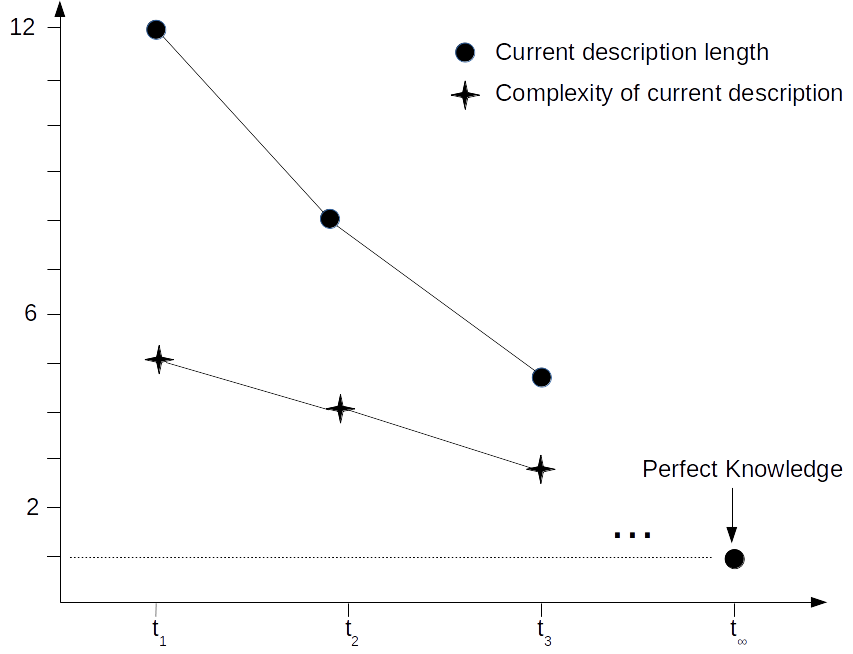
\includegraphics[scale=0.5]{Perfect_Knowledge}
\caption{\label{fig:Perfect_Knowledge}In Pursuit of Perfect Knowledge}
\end{figure}

{\color{red} TODO: Introduce the following definition.}

\begin{definition}
Let $s_{1}, \ldots, s_{n} \in T$ a collection of topics. The \emph{joint nescience} of topics topics $s_{1}, \ldots, s_{n}$ given the current best descriptions $\hat{d_{s_1}}, \ldots, \hat{d_{s_n}}$ is defined as: 
\[
{\color{red} TODO}
\]
\end{definition}

{\color{red} TODO: Mention, or prove, the properties of the generalized nescience}

%
% Current Best Description
%

\section{Current Best Description}

{\color{red} TODO: Rewrite this section}

We are also interested in our current understanding of the concatenation of two topics.

\begin{definition}
Given $t,s \in \mathcal{T}$ two different topics, and the set $\mathcal{D}_{t,s} = \{ d \in \mathcal{B}^\ast, d = \langle TM,a \rangle : TM(a) = \langle t,s \rangle \}$, let $\hat{d}_{t,s}$ be a distinguished element of $\mathcal{D}_{t,s}$. We call $\hat{d}_{t,s}$ our \emph{current best joint description} of $t$ and $s$.
\end{definition}

The concept of best joint description could be a little bit misleading, since given that the concatenation of any two topics is another topic, we could ask ourselves why do not simply use our current best description of the topic represented by that concatenation. That would make sense only in case that somebody has already studied both topics together. However, for the overwhelming majority of the possible combinations of topics, nobody has studied them yet.

\begin{example}
\label{ex:unknown_join}
Let $t$ and $s$ two different topics, and assume that nobody has studied them together before. In this case, our current best description $\hat{d}_{t, s}$ would be $\langle TM, \langle \hat{d}_t, \hat{d}_s \rangle \rangle$, where $TM$ is a Turing machine that given the input $\langle \hat{d}_t, \hat{d}_s \rangle$ prints out the string $ts$. If $\hat{d}_t = \langle TM_t, a_t \rangle$ and $\hat{d}_s = \langle TM_s, a_s \rangle$, the machine $TM$ will decode $\hat{d}_t$, run $TM_t(a_t)$ to print out $t$; then it would do the same for $\hat{d}_s$ to print $s$.
\end{example}

As we said in the preface of this chapter, in order to compute how much we do not know about a topic, first we need a way to quantify what we already know about that topic. How much we know about a topic will be given by our current best known description of that topic.

\begin{definition}
Given the set of descriptions $\mathcal{D}_t$ of a topic $t \in \mathcal{T}$, let $\hat{d_{t}}$ be a distinguished element of $\mathcal{D}_t$. We call $\hat{d_{t}}$ our \emph{current best description} of $t$.
\end{definition}

Which description is the current best description is something that depends on our current knowledge about the particular area in which the theory of nescience is being applied.


%
% Section: Nescience based on Datasets
%

\section{Nescience based on Datasets}
\label{sec:nescience_datasets}

{\color{red} TODO: Perhaps we should remove this section}

Some topics can be described unsing a mathematical model that can
be evaluated by a computer. For those topics we could estimate their
complexity using a sample dataset, for example the result of an experiment.
This property allow us, among other things, to compare how well topics
are described by different models (see Chapter \ref{chap:Structured-Datasets}).

\begin{definition}
Let $t\in T$ be a topic, $D=\left\{ x_{1},x_{2},\ldots,x_{n}\right\} $
the result of running an experiment that describes $t$, and $H$
a mathematical hipothesis for $t$. The complexity of the topic $t$
given the current description $H$ and the dataset $D$ is given by

\[
\hat{C}_{t}=L(H)+L(D\mid H)
\]
as it is described by the minimum description length principle.
\end{definition}

Given the dataset $D$ and the model $H$ we can compute our current
nescience of a topic as it is described by the next definition.

\begin{definition}
Let $t\in T$ a topic, $D=\left\{ x_{1},x_{2},\ldots,x_{n}\right\} $
the result of running an experiment that describes $t$, $C$ a code
that minimizes the length of $D$, and $H$ a mathematical hipothesis
for $t$. The current complexity of the topic $t$ given the dataset
$D$ and the hyphotesis $H$ is given by

\[
N_{t}=\frac{\hat{C_{t}}-l_{C}(D)}{l_{C}(D)}
\]

\end{definition}

In practice, the dataset $D$ also allows us to approximate our current
nescience of a topic $t$, given the model $H$. What we have to do
is to use a near minimal encoding for $D$, for example, by using
a Huffam encoding.


%
% Section
%

\section{Unknonwn Unknown}

{\color{red} TODO: pending}

Knonw unknown

Unknown unknown

Finally, there exists a last category of unknonw, what we call the unknowable unknown unknown. This category refers to those entities we

Unknowable unknown unknonwn. In this book we are interested in the unknown unknown

%
% Section: References
%

\section*{References}

{\color{red} TODO: Add the paper of Chaitin about the Berry paradox}

{\color{red} TODO: That there are numbers that are not computable can be found in the original paper of Turing}

{\color{red} TODO: Perhaps Ii should provide a couple of references in epistemology and ontology}



%
% CHAPTER: The Discovery of Interesting Questions
%

%
% CHAPTER 7.- Interesting Questions
%

%
%  Section 1
%    - (major) We have to clarify which description function we are using
%  Section 4
%    - (major) Missing reference to combined nescience proposition
%

\chapterimage{thinker.pdf}

\chapter{Interesting Questions}
\label{chap:Interesting-Research-Questions}

\begin{quote}
\begin{flushright}
\emph{It is not the answer that enlightens,\\
but the question. \\}
Eugène Ionesco
\end{flushright}
\end{quote}
\bigskip

In this chapter, we propose a set of metrics for classifying research topics based on their potential as a source of interesting problems, along with a methodology for assisted discovery of new questions. The methodology can be used to identify new applications of existing tools to solve open problems and to discover new, previously unexplored research topics. The methodology is applicable to both intradisciplinary and interdisciplinary topics, but the most interesting outcomes are obtained in the latter case. In Chapters \ref{chap:philosophy-science} and \ref{chap:computational-creativity}, we demonstrate the application of the methodology in practice and suggest new questions and research topics.

Our primary assumption is that a research question is interesting if it meets the following three criteria\index{Criteria for Interesting Questions}:

\bigskip

\begin{description}
\item[C1] The question should be new and original, meaning that it has not been previously considered.
\item[C2] Upon its resolution, there should be a significant increase in our knowledge about one or more specific research topics.
\item[C3] It should have practical applications that could have a substantial (hopefully positive) impact on people's lives.
\end{description}

\bigskip

Some researchers may argue that the requirements presented may not be the most suitable. For instance, researchers from the so-called "hard sciences", such as pure mathematics and theoretical physics, might object that practical applications are not a crucial factor in pursuing an interesting open problem. In such situations, the metrics introduced can be redefined since they are simply mathematical abstractions, and the same methods can still be applied. The methodology described is universal and can be employed in various domains, not only in discovering new research questions. In fact, the metrics and methods outlined can be utilized in any field where there is a vast collection of interconnected describable objects, and the objective is to uncover new and previously unknown objects. The precise definition of concepts like relevance graph, applicability graph, or maturity will be contingent on the field in which the approach is being employed. Nevertheless, as in the case of Chapter \ref{chap:Nescience}, we prefer to present the methodology and new concepts in the specific context of scientific research because it aids in their comprehension.

It is worth mentioning the relationship between this new methodology and the areas of computational creativity and artificial intelligence. What is proposed in this chapter is an algebraic approach to the assisted discovery of potentially interesting questions. The intention is not for the computer to understand the meaning of the questions posed. Furthermore, not all the questions generated are necessarily relevant or even meaningful. It is the responsibility of the researchers to assess the proposed combinations of topics and determine if any of the questions are appropriate.

We have already explored two dimensions for classifying topics: miscoding (Chapter \ref{chap:Miscoding}) and mismodel (Chapter \ref{chap:Redundancy}). These metrics enable us to quantitatively assess our understanding of a topic, which we refer to as nescience. According to criterion \textbf{C2} of our list of requirements for questions, the higher the nescience of a topic, the greater its potential as a source of interesting research questions. In this section, we will introduce two additional metrics for characterizing topics: relevance and applicability. Relevance measures the impact a topic has on people's lives and serves as a complement to nescience. Applicability measures how frequently a topic has been applied in other areas and enables us to identify new applications of already existing technologies.

%
% Section: Relevance
%

\section{Relevance}

Before to measure relevance of a topic, that is, its impact in people's life, we have to introduce the concept of \emph{relevance graph}\index{Relevance graph}. The relevance graph is a graph that describes which people is affected by which research topics.

\begin{definition}\index{Relevance Graph}
\label{def:relevance-graph}
We define the \emph{relevance graph}, denoted by $\mathbf{RG}$, as the bipartite graph $\mathbf{RG} = (\mathcal{T}, \mathcal{P}, E)$, where $\mathcal{T}$ is the set of topics, $\mathcal{P}$ the set of people, and $E\subseteq\left\{ \left(i,j\right):i\in \mathcal{T},j\in \mathcal{P} \right\}$ is the set of arcs between topics and people. An arc $(i, j)$ belong to $E$ if, and only if, person $j$ is affected by topic $i$.
\end{definition}

When we refer to the set of people $\mathcal{P}$, we are referring to all individuals in the world. An edge in the relevance graph indicates that someone is affected by a topic, rather than being interested in it. The exact meaning of "being affected by" is a difficult to define concept that is beyond the scope of this book. Therefore, our definition of the relevance graph is a mathematical abstraction. In Section \ref{sec:Classification_Research_Topics}, we will explore how to approximate this quantity in the case of scientific research topics. In Chapter \ref{chap:Software-Engineering}, we will provide an alternative interpretation of the relevance graph in the context of measuring software quality.

\begin{example}
A man who is affected by ALS (amyotrophic lateral sclerosis) disease will be connected to the ALS topic in the graph. His spouse will also be connected because she is likely to be impacted by the consequences of the disease as well. However, a researcher who is interested in ALS as a research problem, rather than someone suffering the disease, will not be connected to the ALS node in the graph.
\end{example}

Optionally, we can add a weight $w_{ij}\in\left[0,1\right]$ to the edges of the graph to specify the degree in which a person $j$ is affected by a topic $i$. A weight of $1$ could represent a life-or-death dependence, and $0$ would mean that this person is not affected at all. In Figure \ref{fig:Relevance-Graph} it is depicted an example of relevance graph. 

\begin{figure}[h]
\centering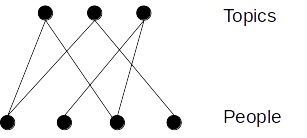
\includegraphics[scale=0.7]{bipartite_graph}
\caption{\label{fig:Relevance-Graph}Relevance Graph}
\end{figure}

\begin{definition}\index{Relevance}
\label{def:relevance}
We define the \emph{relevance} of a topic $t \in \mathcal{T}$, denoted by $R(t)$, as the degree of the node $t$ in the relevance graph, that is, $R(t) = deg(t)$.
\end{definition}

Intuitively, the higher the relevance of a topic, the higher its potential as a source of interesting questions, since we will be working on a problem that affects many people.

Sometimes it is covenient to work with a normalized version of the relevance of a topic.

\begin{definition}\index{Normalized relevance}
\label{def:normalized_relevance}
We define the \emph{normalized relevance} of a topic $t \in \mathcal{T}$, denoted by $\bar{R}(t)$, as the normalized degree of the node $t$ in the relevance graph, that is, $\bar{R}(t) = deg(t) / d(E)$.
\end{definition}

We could have computed also $deg(p)$, that is, the number of edges that links to a person $p$ in the relevance graph, as a measure of the number of topics that affects a particular person. However, this quantity is not used in the theory of nescience. The relation between $deg(t)$ and $deg(p)$ is given by the degree sum formula:
\[
\sum_{t \in \mathcal{T}} deg(t) = \sum_{p \in \mathcal{P}} deg(p) = d(E)
\]

Next proposition proves that adding more topics to a research project can only increase its relevance. Of course, a research project dealing with "life, the universe and everything" would be a highly relevant one, but very impractical as well. How to properly combine research topics will be described in Section \ref{sec:New_Research_Topics}.

\begin{proposition}
\label{prop:nondecreasing_relevance}
Given any two topics $t_{1}, t_{2} \in \mathcal{T}$, we have that $R(t_{1}) + R(t_{2}) \geq R(t_{1})$.
\end{proposition}
\begin{proof}
Let $S_{1}$ the set of people connected to to topic $t_{1}$ in the relevance graph, and  $S_{2}$ the set of people connected to to topic $t_{2}$. Since $d \left( S_{1} \cup S_{2} \right) = d(S_{1}) + d(S_{2}) - d(S_{1} \cap S_{2})$, and $d(S_{2}) - d(S_{1} \cap S_{2}) \geq 0$ we have that $d \left( S_{1} \cup S_{2} \right) \geq d(S_{1})$ and thus $R(t_{1}) + R(t_{2}) \geq R(t_{1})$.
\end{proof} 

Finally, we define the concept of interestingness of a topic as a source of interesting problems, that is, how likely is that the topic can be used in a new interesting research question, as a function of its nescience and relevance. We can visualize topics in a two-dimensional vector space, in which one dimension is nescience, and the other one is relevance. In this interpretation, a natural choice of interestingness function would be the euclidean distance from the origin.

\begin{definition}\index{Interestingness of a topic as a problem}
Given a topic $t \in \mathcal{T}$, we define the \emph{interestingness of the topic as a problem}, denoted by $IP(t)$, as:
\[
IP(t) = \sqrt{ \nu(t)^2 +  R(t)^2 }
\]
\end{definition}

Intuitively, a topic is interesting as a problem worth investigating if it has a large relevance (it has high impact in people's life) and a large nescience (it is not very well understood). In this sense, we are borrowing ideas from Popper's falsificationism: the more risky is a conjecture, the higher the advance achieved in science given its confirmation.

\begin{example}
\label{ex:fixed_point}
The fixed point theorem has some relevance, since people life's can be indirectly affected by its implications, but since it is a very well understood theorem (our nescience is very low), it is not a very interesting research problem by itself.

World War I is a very relevant topic, because it had a huge impact on many people's life, and also it is not very well understood topic, since it takes hundreds of pages to explain its causes, and there is no general agreement among the specialists. So, according to our definition, it is a very interesting research problem.
\end{example}

In practice, it is convenient to work with the normalized version of the relevance metric, so that we can avoid the case that our questions are always related to a small subset of extremely interesting topics.
\[
IP(t) = \sqrt{ \nu(t)^2 +  \bar{R}(t)^2 }
\]

%
% Applicability
%

\section{Applicability}

As mentioned in Example \ref{ex:fixed_point}, the fixed point theorem is not particularly compelling as a research problem on its own. However, it is an essential mathematical result since it has broad applications in proving many other theorems. In this section, we introduce the concept of \emph{applicability}, which is a novel measure enabling us to identify which topics are important since they can serve as as tools for understanding other topics. From a mathematical point of view, we say that a tool can be applied to a topic if the conditional nescience (see Section \ref{sec:conditional_nescience}) of the topic given the tool is smaller that the unconditionall nescience of the topic.

Before to formally define the concept of applicability, first we have to introduce a new bipartite graph that describes which topics has been applied as tools to other topics.

\begin{definition}\index{Applicability graph}
\label{def:applicability-graph}
We define the \emph{applicability graph}, denoted by $AG$, as the directed graph $AG = (\mathcal{T}, E)$, where $\mathcal{T}$ is the set of research topics, and $E\subseteq\left\{ (i,j):i,j\in \mathcal{T} \right\} $. An arc $(i, j)$ belong to $E$ if $N \left( t_i \mid t_j \right) < N \left( t_i \right)$. The weight of the arc $(i, j)$ is given by $w_{ij} = N \left( t_i \right) - N \left( t_i \mid t_j \right)$.
\end{definition}

The applicability graph helps us identify those topics that can be pontentially used as tools to understand other topics. The following defintion formally introduces this idea.

\begin{definition}\index{Applicability}
\label{def:applicability}
Given the applicability graph $AG = (\mathcal{T}, E)$, the \emph{applicability} of a topic $t_i \in \mathcal{T}$, denoted by $A(t_i)$, is defined as the sum of the weights of the arcs in the outdegree of $t_i$, that is:
\[
A(t_i) = \sum_{(i, j) \in E} w_{ij}
\]
where $E$ is the set of arcs in the applicability graph, and $w_{ij}$ is the weight of the arc $(i, j)$.
\end{definition}

A topic with higher applicability will have a greater overall impact on the understanding of other topics, and intuitively, the higher the applicability of a topic, the higher its potential as a tool that can be applied to solve open problems. If a tool has been successfully applied multiple times in the past to address open problems, it is more likely that it can be effectively used to solve other open problems as well.

Next proposition proves that the combination of two topics can only increase their applicability. That is, the more tools we have at our disposal, the more problems we could solve in principle.

\begin{proposition}
Given any two topics $t_1, t_2 \in \mathcal{T}$, we have that $A(t_1) + A(t_2) \geq A(t_1)$.
\end{proposition}
\begin{proof}
Use the same argument than in Proposition \ref{prop:nondecreasing_relevance}.
\end{proof}

In order to better compare the applicability of different topics and understand their relative importance in a standardized way, it is useful to introduce a normalized version of the applicability measure.

\begin{definition}\index{Normalized Aapplicability}
\label{def:normalized-applicability}
Given the applicability graph $AG = (\mathcal{T}, E)$, the \emph{normalized applicability} of a topic $t_i \in \mathcal{T}$, denoted by $A_n(t_i)$, is defined as the ratio of the applicability of $t_i$ to the maximum possible applicability value, expressed as:
\[
\tilde{A}(t_i) = \frac{A(t_i)}{\max_{t_k \in \mathcal{T}} A(t_k)}
\]
where $A(t_i)$ is the applicability of topic $t_i$ as defined in Definition \ref{def:applicability}, and $\max_{t_k \in \mathcal{T}} A(t_k)$ is the maximum applicability value among all topics in $\mathcal{T}$.
\end{definition}

Normalized applicability scales the original applicability value of a topic to a range between 0 and 1, allowing for easier comparison across different topics.

In practice, it is very difficult to compute the applicability graph, since for the majority of the topics, the quantity $N \left( t_i \mid t_j \right)$ has not been estimated. In order to solve this problem, we can use an approximation to the applicabilitiy graph, in which the arcs have no weight, and an edge $(i, j)$ represents that the topic $j$ has been applied to solve the problem $i$. For example, there would be a direct link between the topics "graph theory" and "recommendation engines", since graph theory has been successfully applied to the problem of how to recommend purchase items to customers over Internet.

\begin{definition}\index{Simplified applicability graph}
\label{def:simplified-applicability-graph}
We define the \emph{simplifiled applicability graph}, denoted by $SAG$, as the directed graph $SAG = (\mathcal{T}, E)$, where $\mathcal{T}$ is the set of research topics, and $E\subseteq\left\{ (i,j):i,j\in \mathcal{T} \right\} $. An arc $(i, j)$ belong to $E$ if the topic $j$ has been used to understand topic $i$.
\end{definition}

Using this simplified version of the applicability graph, the concept of applicability becomes:

\begin{definition}\index{Simplified applicability}
\label{def:simplified-applicability}
We define the \emph{simplified applicability} of a topic $t\in \mathcal{T}$, denoted by $SA(t)$, as the outdegree of that node in the applicability graph, that is:
\[
SA(t) = outdeg(t)
\]
\end{definition}

And the corresponding normalized version becomes:

\begin{definition}\index{Normalized simplified applicability}
\label{def:normalized-simplified-applicability}
Given the simplified applicability graph $SAG = (\mathcal{T}, E)$, the \emph{simplified normalized applicability} of a topic $t_i \in \mathcal{T}$, denoted by $SA_n(t_i)$, is defined as the ratio of the simplified applicability of $t_i$ to the maximum possible simplified applicability value, expressed as:
\[
SA_n(t_i) = \frac{SA(t_i)}{\max_{t_k \in \mathcal{T}} SA(t_k)}
\]
where $SA(t_i)$ is the simplified applicability of topic $t_i$ as defined in Definition \ref{def:applicability}, and $\max_{t_k \in \mathcal{T}} SA(t_k)$ is the maximum applicability value among all topics in $\mathcal{T}$.
\end{definition}

When using topics as tools, we are primarily interested in those topics that are better understood. Generally, relying on a background knowledge that is poorly understood is not advisable, even if it significantly reduces the (conditional) nescience of our problem. In the following definition, we will introduce the concept of the maturity of a topic as one minus its nescience.

\begin{definition}\index{Maturity}
Given a topic $t \in \mathcal{T}$, we define the \emph{maturity} of topic $t$, denoted as $M(t)$, as:
\[
M(t) = \nu(t)^{-1}
\]
\end{definition}

Intuitively, the more mature a topic is, the greater its utility in solving other open problems. Highly immature topics should not be applied as tools to address open problems, as doing so would merely transfer our lack of understanding from one topic to another.

\begin{example}
Linear regression is a highly mature topic, since its nescience is very small.
\end{example}

Finally, we define the concept of interestingness of a topic as a source of interesting tools, that is, how likely is that the topic can be used to solve a new problem, as a function of its maturity and applicability. Similar to the definition of relevance introduced in the previous section, topics can be visualized within a two-dimensional vector space, where one dimension represents maturity and the other represents applicability. The interestingness of a topic will be determined by its Euclidean distance from the origin.

\begin{definition}\index{Interestingness of a topic as a tool}
Given a topic $t \in \mathcal{T}$, we define the \emph{interestingness of the topic as a tool}, denoted by $IT(t)$, as:
\[
IT(t) = \sqrt{ M(t)^2 +  A(t)^2 }
\]
\end{definition}

Intuitively, a topic is considered interesting as a tool if it is thoroughly understood and has already been applied to numerous other problems.

\begin{example}
The Pythagorean theorem (in a right-angled triangle, the square of the length of the hypotenuse is equal to the sum of the squares of the other two sides) is undoubtedly one of the most widely used and applied theorems in various fields and practical situations, including but not limited to: engineering (calculating distances, angles, and forces in structures and mechanical systems), architecture (determining lengths and angles in building design and construction projects), land surveying (measuring distances and calculating areas of land parcels), physics (analyzing problems in mechanics, optics, and electromagnetism), computer graphics and game development (calculating distances and angles in 2D and 3D spaces) or trigonometry(serving as a foundation for the study of trigonometric functions and their applications). The widespread application of the Pythagorean theorem to so many fields is due to its simplicity and its ability to describe complex geometric relationships.
\end{example}


%
% Section: Interesting Questions
%

\section{Interesting Questions}

In the quest to uncover novel research questions, combining existing topics from various fields can yield fascinating results. By applying tools and methodologies from one topic to solve problems in another, researchers can explore innovative avenues and potentially make groundbreaking discoveries. In the following section, we delve into the methodology of combining topics to generate questions, along with the concept of interestingness and interdisciplinary research.

In our methdology, a interesting question emerges from the combination of two pre-existing topics. Given a pair of a topics in $t_1, t_2 \in \mathcal{T}$, the question can be framed as "\emph{can we apply the tool described by topic $t_1$ to solve the problem described by topic $t_2$?}".

\begin{definition}\index{Question}
Given two topics $t_1, t_2 \in \mathcal{T}$, a \emph{question}, denoted by $Q_{t_1 \rightarrow t_2}$, is the ordered pair $\left(t_1, t_2\right)$.
\end{definition}

The most intriguing questions emerge when topic $t_1$ exhibits high interestingness as a tool, and topic $t_2$ demonstrates high interestingness as a problem. We define the interestingness of a question using the Euclidean distance, taking into account the interestingness of topics $t_1$ and $t_2$ as points in a two-dimensional space, with coordinates $(A_{t_1}, M_{t_1})$ and $(R_{t_2}, N_{t_2})$, respectively. The coordinates of the resulting vector represent the interestingness of a question with $t_1$ as a tool and $t_2$ as a problem.

\begin{definition}\index{Interestingness of a question}
Let $t_1$ and $t_2 \in \mathcal{T}$ be two topics. The \emph{interestingness} of the question $Q_{t_1 \rightarrow t_2}$, denoted by $IQ_{t_1 \rightarrow t_2}$, is given by:
\[
IQ_{t_1 \rightarrow t_2} = \sqrt{ (A_{t_1} + R_{t_2})^2 + (M_{t_1} + N_{t_2})^2 }
\]
\end{definition}

Employing the Euclidean distance in this way enables a geometric interpretation of the interestingness of a question based on the vector representation of topics in the interestingness space. The larger the magnitude of the vector representation, the higher the interestingness of the resulting question.

\begin{tikzpicture}[
    scale=1.5,
%    axis/.style={thick, ->, -latex', >=Stealth},
    axis/.style={thick},
%   vector/.style={thick, ->, -latex', >=Stealth, color=blue},
    vector/.style={thick},
    point/.style={circle, inner sep=1pt, fill, color=black}
]

% Coordinate axes
\draw[axis] (-0.5, 0) -- (3, 0) node[right] {Interestingness as a Tool (IT)};
\draw[axis] (0, -0.5) -- (0, 3) node[above] {Interestingness as a Problem (IP)};

% Points for t1 and t2
\coordinate (t1) at (1, 1);
\coordinate (t2) at (2, 2);

% Vectors for t1, t2, and the sum
\draw[vector] (0, 0) -- node[pos=0.5, above] {$t_1$} (t1);
\draw[vector] (0, 0) -- node[pos=0.5, below] {$t_2$} (t2);
\draw[vector, color=red] (t1) -- node[pos=0.5, above] {Interestingness of Question} (t2);

% Points and labels for t1 and t2
\node[point, label={left:$A_{t_1}, M_{t_1}$}] at (t1) {};
\node[point, label={right:$R_{t_2}, N_{t_2}$}] at (t2) {};

\end{tikzpicture}

In practice, we must calculate all possible combinations of topics with high interestingness as tools and those with high interestingness as problems. We then select the combinations with the highest interestingness as questions. Naturally, most questions generated using this approach will be meaningless, much like those arising during brainstorming sessions when researchers attempt to identify new tools for tackling difficult problems.

This methodology can be applied in other scenarios as well. For instance, a researcher familiar with problem $p$ might be interested in finding applicable tools to solve it. Similarly, a researcher specializing in tool $t$ may be interested in discovering open problems where his expertise can be applied.

The above procedure can be easily generalized to encompass multiple tools and possibly multiple problems. This leads to the application of two tools to a given problem ($ t_1 + t_2 \rightarrow p$), the application of a single tool to the combination of two problems ($t \rightarrow p_1 + p_2$), and so on. The exact meaning of these tool and problem combinations depends on the topics themselves and is left to the researcher's creative interpretation.

At times, it is beneficial to limit our search to specific areas of knowledge to identify interesting questions.

\begin{definition}\index{Intradisciplinary question} \index{Interdisciplinary question}
Let $\mathcal{A} \subset \mathcal{T}$ be a research area, and $t_1, t_2 \in \mathcal{T}$ be two topics. If both topics belongs to the same area, meaning $t_1, t_2 \in \mathcal{A}$, we say that the question $Q_{t_1 \rightarrow t_2}$ is \emph{intradisciplinary}, otherwise, we say that the question is \emph{interdisciplinary}.
\end{definition}

The most innovative questions tend to be interdisciplinary, as they have a lower likelihood of having been considered previously. This is because they require collaboration between specialists from different research areas. Interdisciplinary questions address our requirement \textbf{C1} for interesting questions, which dictates that the question must be new and original.

%
% Section: New Research Topics
%

\section{New Research Topics}
\label{sec:New_Research_Topics}

{\color{red} TODO: Review this section}

In the previous section our focus was in how to find new interesting research questions. In this section we will go one step beyond, and we will show how to identify new, previously unknown, research topics.

\begin{definition}\index{Unknown frontier}
In the two-dimensional space defined by relevance and nescience, the \textit{unknown frontier}, denoted by $\mathbb{F}$, is defined as the following arc:
\[
\mathbb{F} = \left\{(x,y) \mid x^{2}+y^{2}=max(\{N^2_{t} + R^2_{t}, t \in T'\}),x>0,y>0\right\} 
\]
\end{definition}

If we plot all the known research topics according to their relevance and nescience, the unknown frontier will cover them. Intuitively the \emph{unknown frontier} marks the frontier between what we do not know and we are aware that we do not know (we do not fully understand those topics), and what we do not known and we are not yet aware that we do not known those topics. This intuitive property is in general terms, since it may happen that some unknown topics lie under the unknown frontier as well.

\begin{definition}\index{New topics area}
Lets $T'$ the set of known research topics. The \emph{new topics area}, denoted by $\mathbb{S}$, is defined by:
\[
\mathbb{S} = \left\{(x,y) \mid x^{2}+y^{2}>max(\{N^2_{t} + R^2_{t}, t \in T'\}),x>0,y>0\right\} 
\]
\end{definition}

The new topics area contains all those unknown topics that we are not aware we do not know them (unknown unknown). The big issue is how to reach this new topics area if we do not know anything about the topics included in that area.

\begin{proposition}
\label{prop:new-topics-area}
Let $r \in T$ be a topic, if  $N^2_{r} + R^2_{r} > max(\{N^2_{t} + R^2_{t}, t \in T'\}$ then $t \in T \setminus T'$.
\end{proposition}
\begin{proof}
Let $N^2_{r} + R^2_{r} > max(\{N^2_{t} + R^2_{t}, t \in T'\}$ and suppose that $r \in T'$, then have that $max(\{N^2_{t} + R^2_{t}, t \in T'\}) \geq N^2_{r} + R^2_{r}$ that it is a contradiction, and so $t \in T \setminus T'$.
\end{proof}

Proposition \ref{prop:new-topics-area} together with the fact that the combined nescience of two topics is higher than the nescience of any of them isolated (Proposition {\color{red} XXX}), and that their combined relevance is higher that the relevance of any of them (Proposition \ref{prop:nondecreasing_relevance}), a possible approach to identify new topics could be by means of combining already existing interesting problems. In Figure \ref{fig:New-Topics} is depicted graphically the idea.

\begin{figure}[h]
\centering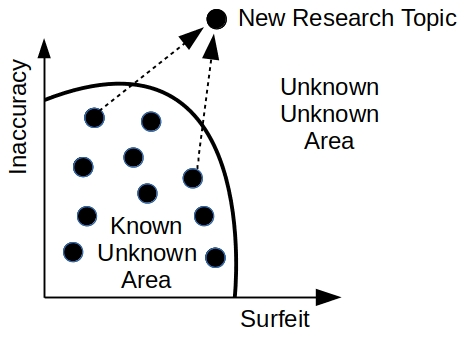
\includegraphics[scale=0.4]{NewTopics}
\caption{\label{fig:New-Topics}The discovery of new research topics}
\end{figure}

\begin{definition}\index{New topic}
Given two topics $t_{1}, t_{2} \in T'$, a \emph{new topic}, denoted by $S_{\left\{ t_{1},t_{2}\right\}}$, is the unordered pair $\left\{ t_{1},t_{2}\right\}$.
\end{definition}

The exact meaning of the new topic that results as the combination of topics $t_{1}$ and $t_{2}$ is left to the creative interpretation of the researcher.

\begin{definition}\index{Interestingness of a new topic}
The \emph{interestingness} of the new topic, denoted by $IS_{\left\{ t_{1},t_{2}\right\} }$, is given by:
\[
IS_{\left\{ t_{1},t_{2}\right\} } = R_{t_{1}}R_{t_{2}}+N_{t_{1}}N_{t_{2}}
\]
\end{definition}

In practice, what we have to do is to compute all possible combination of those topics with very large interestingness as problems $IP_{t}$ with themselves, and select the combinations with higher $IS$. Of course, some of the combinations generated would be totally meaningless. Advanced techniques from the area of natural language processing or machine learning could be used to try filter out those nonsense combinations.

\begin{definition}\index{Intradisciplinary new topic} \index{Interdisciplinary new topic}
Let $A \subset T$ a research area, and $t_{1}, t_{2} \in T$ two topics. If both topics belongs to the same area, that is $t_{1}, t_{2} \in A$, we say that the new topic $S_{\left\{ t_{1},t_{2}\right\} }$ is \emph{intradisciplinary}, otherwise, we say that the topic is \emph{interdisciplinary}.
\end{definition}

Again, the most innovative new topics would be by the combination of interdisciplinary topics, because the probability that somebody has already though about them is lower.

%
% Section: Classification of Research Areas
%

\section{Classification of Research Areas}

In the same way we studied the nescience of research areas (see Section \ref{sec:nescience_areas}), we could also study the interestingness of research areas.

\begin{definition}\index{Average interestingness of an area}
Given a research area $A\subset T$, we define the \emph{average interestingness
of the area as a source of interesting tools} by
\[
IT_{A}=\frac{1}{n}\sum_{t\in A}IT_{t}
\]
and the \emph{average interestingness of the area as a source of interesting
problems} by
\[
IP_{A}=\frac{1}{n}\sum_{t\in A}IP_{t}
\]
where $n$ is the cardinality of $A$.
\end{definition}

In this way we could compute the interestingness of mathematics, physics, biology, social sciences, and other disciplines as a source of interesting tools and problems. Other alternative measures of centrality and dispersion could be used for the characterization of research areas as well.

As I will show in Chapter \ref{chap:The-Scientific-Method}, the interestingness of mathematics as a source of tools is higher than the interest of social sciences, since mathematics is composed of topics with a high applicability that are very well understood, and that is not the case, in general, for social sciences. On the other hand, the interestingness of social sciences as a source of problems is higher than the interest of mathematics, since the topics studied by the social sciences are more relevant to humankind \footnote{Please mind that I am not saying that the topics addressed by mathematics are not relevant to humankind, what I am saying is that, in relative terms, the problems addressed by social sciences have a higher relevance.} and, in general, not very well understood.

\begin{example}\index{Areas in decay}
We could use the interestingness of an area to identify research areas in decay. A knowledge area is in decay (from the research point of view) if it has no enough interesting research problems. For example, although the aerodynamics of zeppelins is not fully understood (still some nescience), it is not longer useful (low relevance), since people does not use zeppelins to travel anymore, and so, the average interestingness is very low. Another example of area in decay is classical geometry: although it is relevant, our understanding of this subject is nearly perfect, since there are almost no unsolved problems, and so, its average nescience is very low. However, on the contrary to what happens in case of the aerodynamics of zeppelins, classical geometry is still very interesting as a source of tools.
\end{example}

It is worth to mention that we could add other metrics to provide a finer, or even alternative, characterization of the unknown unknown area. For example, we could add to nescience and relevance a third dimension with the probability that a topic description is true. However, these extended or alternative characterizations will be not considered in this book. Fortunately, the idea of how to reach the unknown unknown area is the same, regardless of the number and the metrics used (as long as these metrics satisfy some minimal mathematical properties, described in Chapters \ref{chap:Nescience} and \ref{chap:Interesting-Research-Questions}).

%
% References
%

\section*{References}

Popper and falsificationism

{\color{red} Review the following references}

\begin{itemize}

\item Freitas, A. A. (1999). On Objective Measures of Rule Surprisingness. In Proceedings of the Second European Symposium on Principles of Data Mining and Knowledge Discovery (PKDD '98), pp. 1-9.

\item Gureckis, T. M., \& Goldstone, R. L. (2009). How You Named Your Child: Understanding The Relationship Between Individual Decision Making and Collective Outcomes. Topics in Cognitive Science, 1(4), 651-674.

\item Klein, J. T. (1990). Interdisciplinarity: History, Theory, and Practice. Wayne State University Press.

\item Kuhn, T. S. (1962). The Structure of Scientific Revolutions. University of Chicago Press.

\item Newell, A., \& Simon, H. A. (1972). Human Problem Solving. Prentice-Hall.

\item Page, S. E. (2007). The Difference: How the Power of Diversity Creates Better Groups, Firms, Schools, and Societies. Princeton University Press.

\item Rescher, N. (1986). The Riddle of Existence: An Essay in Idealistic Metaphysics. University Press of America.

\item Schelling, T. C. (1978). Micromotives and Macrobehavior. W. W. Norton \& Company.

\end{itemize}


%
% CHAPTER: Advanced Properties of Nescience
%

%
% CHAPTER 8.- Properties of Nescience
%

\chapterimage{Philosophers.pdf}

\chapter{Advanced Properties}
\label{chap:Properties-Nescience}

\begin{quote}
\begin{flushright}
\emph{Invert, always invert.}\\
Carl Gustav Jacob Jacobi\\
\end{flushright}
\end{quote}
\bigskip

This chapter covers more advanced mathematical properties of the concept of nescience. This chapter can be safely skipped by those readers interested only in the applications of nescience. However, it is highly recommended to read it, since if provides a deeper understanding of what nescience is exactly.

{\color{red} TODO: Explain the abstract nature of the axioms vs. the interpretation we have provided in the previous chapters. Mention that perhaps there exists other interpretations.}

Since the time of David Hilbert, mathematics is about the study of the properties of abstract objects and their relations, without paying too much attention to what these objects are or represent. Mathematicians create (or discover) abstract frameworks of logic that can have multiple interpretations. It is up to applied scientists to provide those interpretations. In the same way, we can provide an abstract definition of the concept of nescience, and study its properties, without making any explicit reference to science nor to the scientific method. In doing so, we loose the interpretability of our theory, but, on the other side, we could apply the same results to other disciplines.

{\color{red} Extend this introduction with a very short review of the topics covered in the chapter.}

%
% Section: Axioms
%

\section{The Axioms of Science}

In this section we are going to propose a collection of axioms that formalize what is science. Our axioms are based on first-order logic and the ZFC axioms of set theory with equality (see Appendix \ref{apx:foundations_mathematics}). We will also prove some basic results and explain how these axioms match the new ideas we have introduced in this book. In our axiomatization we are not going to follow the approach described in the previous chapters, that is, we are not going to explicitly definine the quantities of miscoding, surfeit and inaccuracy. Instead, we will introduce the junction and conditional operations, list their fundamental properties, and explain how nescience is afected by them. The remaining concepts follow from these basic axioms.

\begin{definition}

Let $\mathcal{B}^\ast$ be the set of all finite binary strings. We define \emph{science} as the first-order logic structure $(\mathcal{B}^\ast \mid \lambda, \mathcal{O}, <_N, \oplus, \mid)$ where:

\vskip 0.25cm

\begin{enumerate}[label=(\roman*)]
\item $\lambda \in \Sigma$ is the empty string.
\item $\mathcal{O}$ is a relation called \emph{oracle},
\item $<_N$ is a relation called \emph{nescience},
\item $\oplus$ is a binary function called \emph{joint}, and
\item $\mid$ is a binary function called \emph{conditional}
\end{enumerate}

\vskip 0.25cm

that satisfies the following axioms:

\vskip 0.25cm

\begin{itemize}

% Oracle
\item[A1] $\forall t \in \mathcal{B}^\ast \; t \mathcal{O} t$.
\item[A2] $\forall s , t \in \mathcal{B}^\ast$ if $s \mathcal{O} t$ then $t \mathcal{O} s$.
\item[A3] $\forall r, s , t \in \mathcal{B}^\ast$ if $r \mathcal{O} s$ and $s \mathcal{O} t$ then $r \mathcal{O} t$.

\vskip 0.25cm

% Nescience
\item[A4] $\forall t \in \mathcal{B}^\ast$ $\lnot t <_N t$.
\item[A5] $\forall s , t \in \mathcal{B}^\ast$ if $s <_N t$ then $\lnot t <_N s$.
\item[A6] $\forall r , s, t \in \mathcal{B}^\ast$ if $r <_N s$ and $s <_N t$ then $r <_N t$.

\vskip 0.25cm

% Concatenation
\item[A8] $\forall s, t \in \mathcal{B}^\ast$ $\oplus(s, t) \in \mathcal{B}^\ast$.
\item[A9] $\forall s \in \mathcal{B}^\ast$ $\oplus(s, \lambda) = \oplus( \lambda, s) = s$.
\item[A10] $\forall r, s, t \in \mathcal{B}^\ast$ $\oplus(\oplus(r, s), t) = \oplus(r, \oplus(s, t))$.

\vskip 0.25cm

% Conditional
\item[A11] $\forall s \in \mathcal{B}^\ast$ $\mid (s, \lambda) = s$.
\item[A12] $\forall s, t \in \mathcal{B}^\ast$ $\lnot s <_N \mid (s, t)$

\end{itemize}

\end{definition}

Axioms A1, A2 and A3 state that the oracle $\mathcal{O}$ is an equivalence relation that partitions the set of strings into entities. The nescience relation $<_N$, described by Axioms A4, A5 and A6 is a strict partial order that compares the relative unknowns of pairs of strings. The concatenation operation $\oplus$ of Axioms A8, A9 and A10 contains the usual properties of the contatenation of strings, and together with $\mathcal{B}^\ast$ forms a free monoid. Axioms A11 and A12 define the behaviour of the conditional operator $\mid$. 

We still need two more axioms to fully characterize the behaviour of the nescience function. But fist we have to introduce some additional definitions and notations.

\begin{definition}
Let $\mathcal{B}^\ast / \mathcal{O}$ be the quotation set defined by the oracle relation over the set of strings. We call \emph{entity}, denoted by $[e]$, to every class of this quotation set, that is, $[e] \in \mathcal{B}^\ast / \mathcal{O}$.
\end{definition}

We require that every entity contains at least one minimal string with respect to the nescience ordering.

\begin{definition}[Axiom A13]
For every entity $[e] \in \mathcal{B}^\ast / \mathcal{O}$ there exists at least one $r \in [e]$ such that it is minimal with respect to $<_N$, that is, it does not exists an $s \in [e]$ such that $s <_N r$.
\end{definition}

An entity can have more than one minimal element. The axioms do not require the nescience relation to have a global minimum element for $\mathcal{B}^\ast$, nor minimum elements for the individual equivalence classes.

The following notational convention is introduced to simplify the algebraic operations dealing with nescience.

\begin{notation}
We will use the infix notation for the concatenation function, that is, we will write $s \oplus t$ instead of the $\oplus(s, t)$. Moreover, given Axiom A10, we will drop parenthesis in case of multiple concatenations.

We will use the infix notation for the conditional function, that is, we will write $s \mid t$ instead of the $\mid(s, t)$.
\end{notation}

Our last axiom explains how we can decrease the nescience of a given a particular entity.

\begin{definition}[Axiom A14]
Let $t \in \mathcal{B}^\ast$ be a non-minimal element, then at least one of the following is true:
\begin{enumerate}[label=(\roman*)]
\item there exist $s \in \mathcal{B}^\ast$ such that $s \oplus t <_N s$ or $t \oplus s <_N t$,
\item there exists $s, \alpha, \beta \in \mathcal{B}^\ast$ in the form $t = \alpha \oplus s \oplus \beta$ such that $s <_N t$,
\item there exists $s \in \mathcal{B}^\ast$ such that $t \mid s <_N t$.
\end{enumerate}
\end{definition}

It is convenient to introduce the symbol $=_N$ to represent the case that our unknown given the strings $s$ and $t$ is the same. This can be done only if both strings belong to the same equivalence class.

\begin{notation}
Let $[e]$ be an entity, and $s, t \in [e]$ two strings. We denote by $ s =_N t$ the case that $(s, t) \notin <_N$.
\end{notation}

Concatenation is intended to capture the concept of creativity in the theory of nescience. Next axiom proves this capability.

\begin{proposition}
\item[Axiom XX] Let $[e]$ be an entity, and $t \in [e]$ and $s \notin [e]$ two arbitrary strings, then we have that $s <_N \oplus(s, t)$ and $t <_N \oplus(s, t)$.
\end{proposition}
\begin{proof}
{\color{red} TO DO}
\end{proof}

\begin{proposition}
{\color{red} TODO: Explain how concatenation and conditional can be combined into a single equation, something like a distributive law.}
\end{proposition}

{\color{red} TODO: Prove that the concatenation of two minimal elements of the same class is also minimal.}

{\color{red} TODO: Properties of the Oracle: projection function, ...}

{\color{red} TODO: Explain what happens with $\lambda$, the class it belongs to, and its role as a minimal element.}


{\color{red} TODO: Prove that there is an isomorphism between set of finite binary strings and the set of natural numbers. The same for a set of non-binary strings.}

{\color{red} TODO: Prove the invariance theorem, that is, changing the oracle (the equivalence relation) does not changes the order of the strings in terms of the nescience.}

%
% Things to cover in the interpretation
%

\subsection{Interpretation of the Axioms}

The axioms of nescience do not expliclty mention the concepts of miscoding, inaccuracy and surfeit. However, there is a natural interpretation of these concepts under these axioms.


Oracle: Each equivalence class corresponds to an entity, and it contains all possible representations
and descriptions of that entity, including the wrong ones. Fron an axiomatic point of view,
reprsentations and descriptions are indistinguishable. The entities themselves are not part of the
set. This abstract oracle is the only tool we have at our disposal to match entities and their
string based representations. The actual schema used internally by the oracle to relate entities and
its representations is irrelevant in this axiomatization. All possible strings belong to at least on
entity, and one string cannot be part of two entities.

We cannot provide a quantitative measure of nescience, since numbers are not part of our
axiomatic structure. Although binary strings can be equaled to natural numbers, the symbols +
and  are missing in our logic structure. Instead what we have defined is a relative ordering of
the different elements of B according to how much we do not known given those strings. The
ordering has to be partial, i.e. not every pair of elements of B can be compared. This partial order
is applicable not only in case of strigs that belong to different entities, but also when they belong to
the same entity. Intra-entity order strictness leads to the notion of nescience Pareto frontier. The
order has to be strict, i.e. nescience equality is not defined. The problem of assuming a non-strict
total order for nescience N is that if s N t and t N s then s = t, that is, if two strings have the
same nescience, they must be the same string, and this is not necessarily the case. Within our
axioms, nescience equality is just a notational convention.

Concatenation is the process that allow us to discover new entities: concatenating two strings
that belong to different entities might lead to a new, previously unknown, entity. Concatenation
implements the exploration part in this schema of exploration/exploitation in which science is
characterized.

%
% Axioms based on Type Theory
%

\subsection{Type Theory}

In the previous section we have provided a formalization of the theory of nescience based in set theory and first order logic. Set theory is not the only available framework in which mathematics can be formalized. We could have used type theory or category theory instead. Having meaniful axioms of our theory in multiple formalization frameworks, such as set theory, type theory, and category theory, will constitute strong evidence that nescience is a fundamental concept in mathematics, and not a mere artifact of a particular formalization.

In this section we are going to provide a formalization of the theory of nescience in the context of type theory (see Section \ref{sec:lambda_calculus}). Type theory has some advantages over set theory. The most important is that it is a constructive theory, which means that we do not assume the existence of abstract mathematical entities that satisfy some properties, but we show how to construct those entities. For example, there is no need to resort to an abstract, uncomputable, oracle. In type theory, all propositions and proven theorems have an equivalent computable function or algorithm, and thus, we can provide computer programs to solve all problems addressed by our theory (see Section \ref{sec:nescience_library} for a practical implementation of some of these algorithms in the form of a software library).

A second advantage of type theory is that the lambda terms used in the theory are by definition computable functions, and that lambda calculus is a Turing machine capable of universal computation. In the theory of nesciece we require that our models be lambda terms, and that our universal Turing machine be the lambda calculus. In this sense, our models are native elements within the theory, not external artifacts based on an arbitrary, axiomatically defined, universal machine. The models that describe entities are lambda terms executed in the univeral Turing machine of lambda calculus.

The third advantage is that there are software implementations of type theory, such as the Coq proof assistant (see Section \ref{apx:coq}), which allow us to mechanically verify the correctness of our theory. In the rest of this section, we will use the coq syntax for definitions, propositions and theorems so that interested readers can use a computer and a Coq interpreter to verify by themselves that the proofs are correct. We have also included an appendix where we briefly describe the Coq language, so that those readers who prefer traditional mathematics can translate the Coq scripts into classical mathematical definitions and propositions.

% Foundamental Concepts

\subsubsection*{Foundamental Concepts}

We start by introducing a new type, called \texttt{String}. The type string is defined recursively in the following way: the empty string, called \texttt{lambda}\footnote{Do not confuse the $\lambda$ symbol with a $\lambda$-term.}, is a string, and the sucessor of a string, given the function \texttt{S}, is also a string. For us strings are just a list of lambdas, and our theory is based on the collection of all finite strings $\{ \lambda, \lambda \lambda, \lambda \lambda \lambda, \ldots \}$. Both descriptions and representations will be finite strings of lambdas.

\begin{sourcecode}
{\scriptsize \begin{verbatim}
Inductive String : Set :=
  | lambda : String
  | S      : String -> String.
\end{verbatim}}
\end{sourcecode}

Before to introduce the main concepts of the theory of nescience, we have to define a helper funcion called \texttt{Difference}. The \texttt{Difference} function computes the absolute difference between two strings, that is, the excess of lambdas of the longer string with respect to the shortest one. For example, if we have the strings $\lambda \lambda$ and $\lambda \lambda \lambda$, the difference would be the string $\lambda$. Given two strings $r$ and $s$, \texttt{Difference} is defined recursively as:

\begin{sourcecode}
{\scriptsize \begin{verbatim}
Fixpoint Difference (r s : String) : String :=
  match r, s with
  | lambda, lambda  => lambda
  | lambda, s       => s
  | r     , lambda  => r
  | S r'  , S s'    => Difference r' s'
  end.
\end{verbatim}}
\end{sourcecode}

We say that a string $r$ has smaller \emph{surfeit} than a string $s$ if the string $r$ is shorter, in terms of number of lambdas, than the string $s$. Given two strings $r$ and $s$, the \texttt{Surfeit} function is defined recursively, and returns \texttt{true} if the string $r$ has less lambdas than the string $s$.  Applied to descriptionss, we prefer those with the smaller number of lamdas.

\begin{sourcecode}
{\scriptsize \begin{verbatim}
Fixpoint Surfeit (r s : String) : bool :=
  match r, s with
  | lambda, lambda => false
  | lambda, _      => true
  | _     , lambda => false
  | S r', S s'     => Surfeit r' s' 
  end.
\end{verbatim}}
\end{sourcecode}

The \emph{inaccuracy} of a string $r$ with respect to a target string $t$ is based on the absolute difference between the two strings, that is, how close is the string to the target. Given two strings $r$ and $s$, and a target string $t$, the \texttt{Inaccuracy} function returns \texttt{true} if the absolute difference between the strings $r$ and $t$ contains less lambdas than the absolute difference between the strings $s$ and $t$. Inaccuracy will be applied to the ouput of the models.

\begin{sourcecode}
{\scriptsize \begin{verbatim}
Definition Inaccuracy (r s : String) (t : String) : bool :=
  Surfeit (Difference r t) (Difference s t).\end{verbatim}}
\end{sourcecode}

\emph{Nescience} will be based on the concepts of surfeit and inaccuracy. Intitively, we are looking for very short descriptions (low surfeit) and with very low error (low inaccuracy). The \texttt{Nescience} function gets as input five strings: $mr$, $ms$, $r$, $s$ and $e$, and returns \emph{true} if $mr$ is a shorter string than $ms$, and the inaccuracy of $r$ is smaller than the inaccucay of $s$ with respect to $e$. Intuitively, $mr$ and $ms$ would be a string-based representations of our models (in our case, lambda-terms), $r$ and $s$ are the string-based outputs of these models, and $e$ is a string-based representation of an entity.

\begin{sourcecode}
{\scriptsize \begin{verbatim}
Definition Nescience (mr ms : String) (r s : String) (e : String) : bool :=
  andb (Surfeit mr ms) (Inaccuracy r s e).
\end{verbatim}}
\end{sourcecode}

In practice, we generally do not know a string-based representation $e$ of the entity we are interested in, so an indirect approach must be used to study that entity. \emph{Miscoding} is this approach, and it will be introduced in a later section.

Instead of defining the new type \texttt{String} we could have reused the concept of natural number, that is, we could have introduced descriptions and representations as numbers. In that case, the \texttt{Difference} between two strings $r$ and $s$ would be the absolutute difference $\mid r - s \mid$ between the numbers $r$ and $s$, and the \texttt{Surfeit} could be based on the the strict order relation between numbers $<$. The concepts of \texttt{Inaccuracy} and \texttt{Nescience} would have been defined in the same way with numbers. However, natural numbers require additional properties that are not needed for the theory of nescience. For example, the multiplication of two natural numbers does not make any sense in our theory.  Reusing natural numbers would have made our theory unnecerarily complex.

In the rest of this section, we will see how we can derive our theory of nescience using only these fundamental concepts. We will also prove the most significant results and derive algorithms for applying the theory in practice.

% Surfeit

\subsubsection*{Surfeit}

Surfeit allow us to compare two strings. Recall that the surfeit of two strings $r$ and $s$ is true if, and only if, $s$ is composed by more lambdas than $r$. Surfeit allow us to order the models (string based representations of the models) by its length. We are interested in those models with the lowest possible complexity. In the rest of this section we are going to review the properties of surfeit.

The surfeit of a string does not increases when we conditions that string to another one. Intuitively, assuming some previous background knowledge already known as true allow us to reduce the complexity of our models.

\begin{sourcecode}
{\scriptsize \begin{verbatim}
Proposition SurfeitConditional : forall r s : String, 
  Surfeit r (r |c s) = false.
Proof.
intros.
induction r as [| r' IHr'].
- simpl.
  reflexivity.
-
Admitted.
\end{verbatim}}
\end{sourcecode}

From a theoretical point of view, the limit to the proccess of conditioning would be to assume as true the current model.

\begin{sourcecode}
{\scriptsize \begin{verbatim}
Proposition SurfeitConditionalLambda : forall r s: String, 
  Surfeit lambda (r |c r) = false.
Proof.
Admitted.
\end{verbatim}}
\end{sourcecode}

The surfeit of a string does not decreases when it is concatenated with another string. Intuitively, the concatenation of two models increases our uknown. This process of concatenating models can be used as an exploratory mechanism to discover new research topics (previously unknown entities).

\begin{sourcecode}
{\scriptsize \begin{verbatim}
Proposition SurfeitConcatenation : forall r s : String, 
  Surfeit r (r <+> s) = false.
Proof.
intros.
Admitted.
\end{verbatim}}
\end{sourcecode}

From the point of view of surfeit, the operation of concatenation can be distributed over the operation of conditioning, as next proposition shows ({\color{red} TODO: provide the intuition behind this distributive law}).

\begin{sourcecode}
{\scriptsize \begin{verbatim}
Proposition DistributiveLawSurfeit : forall r s t  : String,
  Surfeit ((r |c s) <+> t) ((r <+> t) |c (s <+> t)) = true.
Proof.
Admitted.
\end{verbatim}}
\end{sourcecode}

% Inaccuracy

\subsubsection*{Inaccuracy}

{\color{red} Definition and results about inaccuracy}

{\color{red} Inaccuracy does not increases with conditional}

\begin{sourcecode}
{\scriptsize \begin{verbatim}
Proposition InaccuracyConditional : forall r s e : String, 
  Inaccuracy r (r |c s) e = false.
Proof.
Admitted.
\end{verbatim}}
\end{sourcecode}

{\color{red}  The limit would be conditioning a string to itself}

\begin{sourcecode}
{\scriptsize \begin{verbatim}
Proposition InaccuracyConditionalLambda : forall r s: String, 
  Inaccuracy lambda (r |c r) = false.
Proof.
Admitted.
\end{verbatim}}
\end{sourcecode}

{\color{red} Distributive Law}

\begin{sourcecode}
{\scriptsize \begin{verbatim}
Proposition DistributiveLawInaccuracy : forall r s t  : String,
  Inaccuracy ((r |c s) <+> t) ((r <+> t) |c (s <+> t)) = true.
Proof.
Admitted.
\end{verbatim}}
\end{sourcecode}

% Entities, Representations and Descriptions

\subsubsection*{Entities, Representations and Descriptions}

After we have described the fundamental concepts of the theory of nescience, in this section we are going to introduce the remaining elements of the theory, that is, the concepts of entity, representation and description.

We introduce the concept of \emph{entity} recursively as a finite list of strings. Those strings correspond to the valid representations of the entity. We consider that the empty entity, denoted by \emph{nil}, is also an entity.

\begin{sourcecode}
{\scriptsize \begin{verbatim}
Inductive Entity : Set :=
  | nil       : Entity
  | add_repr : String -> Entity -> Entity.
\end{verbatim}}
\end{sourcecode}

A \emph{universe} is a finite list of entities. A universe correspond to the particular reasearch area in which we are interested. We consider that the empty universe, denoted by \emph{empty}, is also a universe. The recursive definition of universe is given by:

\begin{sourcecode}
{\scriptsize \begin{verbatim}
Inductive Universe : Set :=
  | empty      : Universe
  | add_entity : Entity -> Universe -> Universe.
\end{verbatim}}
\end{sourcecode}

A description is a pair composed by a recursive funcion (a $\lambda$-term) from strings to strings, what we call a \emph{model}, and an input string to that model.

\begin{sourcecode}
{\scriptsize \begin{verbatim}
Definition Description (model : String -> String) (input : String) : String :=
  model input.\end{verbatim}}
\end{sourcecode}

% Miscoding

\subsubsection*{Miscoding}

{\color{red} Definition and results about miscoding}


% Properties of Strings

\subsubsection*{Properties of Strings}

Before we move into the details of the theory of nescience, we are going to prove some basic properties that our concept of string satisfies. Also, besides to the already introduced concept of string difference, we are going to introduce two other strings operators: concatenation and conditional.

We say that two strings are \emph{equal} if, and only if, they have the same number of sigmas. String equality is defined recursively as follows:

\begin{sourcecode}
{\scriptsize \begin{verbatim}
Fixpoint Equality (r s : String) : bool :=
  match r, s with
  | lambda, lambda => true
  | lambda, _      => false
  | _     , lambda => false
  | S r'  , S s'   => Equality r' s'
  end.
\end{verbatim}}
\end{sourcecode}

It is convenient to introduce a new infix operator to represent the string equality concept. That will helps us to simplify new definitions and proofs.

\begin{sourcecode}
{\scriptsize \begin{verbatim}
Notation "x =? y"  := (Equality x y)
\end{verbatim}}
\end{sourcecode}

In the same way, we introduce another infix operator to represent the concept of string difference.

\begin{sourcecode}
{\scriptsize \begin{verbatim}
Notation "x <d> y"  := (Difference x y)
\end{verbatim}}
\end{sourcecode}

Strings with the difference operator form an abelian group. That is: it has a neutral element, it is conmutative, associative and has an inverse element.

The neutral element for strings is the $\lambda$ symbol. That $\lambda$ is the neutral elment with respect to the operation of difference is a direct consequence of the definitions of string and difference.

\begin{sourcecode}
{\scriptsize \begin{verbatim}
Proposition DifferenceNeutral : forall r : String,
  r <d> lambda = r /\ lambda <d> r = r.
Proof.
intros.
split.
- destruct r.
  * reflexivity.
  * reflexivity.
- destruct r.
  * reflexivity.
  * reflexivity.
Qed.
\end{verbatim}}
\end{sourcecode}

The property of being conmutative of the difference operator is proved by ... {\color{red} TODO}

\begin{sourcecode}
{\scriptsize \begin{verbatim}
Proposition DifferenceConmutative : forall r s : String,
  r <d> s = s <d> r.
Proof.
Admitted.
\end{verbatim}}
\end{sourcecode}

In the same way, the property of being conmutative is shown by ... {\color{red} TODO}

\begin{sourcecode}
{\scriptsize \begin{verbatim}
Proposition DifferenceAsociative  : forall r s t  : String,
  r <d> (s <d> t) = (r <d> s) <d> t.
Proof.
Admitted.
\end{verbatim}}
\end{sourcecode}

Given an arbitrary string $r$, its inverse element is the string itself, as next proposition shows. The proposition is proved by induction over $r$.

\begin{sourcecode}
{\scriptsize \begin{verbatim}
Proposition DifferenceInverse : forall r : String,
  r <d> r = lambda.
Proof.
intros.
induction r as [| r' IHr'].
- reflexivity.
- simpl.
  apply IHr'.
Qed.
\end{verbatim}}
\end{sourcecode}

The operation of \emph{concatenation} of two strings returns a new string composed by one of the strings appened at the end of the other. The operation of concatenation is defined recursively as:

\begin{sourcecode}
{\scriptsize \begin{verbatim}
Fixpoint Concatenate (r s : String) : String :=
  match r, s with
  | lambda, _     => s
  | S r'  , _     => S (Concatenate r' s)
  end.
\end{verbatim}}
\end{sourcecode}

The infix notation for the concatenation operation is given by:

\begin{sourcecode}
{\scriptsize \begin{verbatim}
Notation "x <+> y" := (Concatenate x y)
\end{verbatim}}
\end{sourcecode}

The pair composed by strings and the concatenation operation form a conmutative monoid. That is, it has a neural element, and it satisfies the properties of being conmutative and associative.

The neutral element of the operation of concatenation is $\lambda$. In order to prove that $\lambda$ is indeed the neutral element we ... {\color{red} TODO}

\begin{sourcecode}
{\scriptsize \begin{verbatim}
Lemma s_plus_lambda : forall s : String,
  s <+> lambda = s.
Proof.
intros.
induction s as [| s' IHs'].
- simpl.
  reflexivity.
- simpl.
  rewrite -> IHs'.
  reflexivity.
Qed.
\end{verbatim}}
\end{sourcecode}

Given the above lemma we can now prove that $\lambda$ is the neutral element ... {\color{red} TODO}

\begin{sourcecode}
{\scriptsize \begin{verbatim}
Proposition ConcatenationNeural : forall r : String,
  r <+> lambda = r /\ lambda <+> r = r.
Proof.
Admitted.
\end{verbatim}}
\end{sourcecode}

{\color{red} TODO: string concatenation is conmutative, and its proof requires to additional lemmas.}

\begin{sourcecode}
{\scriptsize \begin{verbatim}
Lemma plus_r_Ss : forall r s: String,
  S (r <+> s) = r <+> S s.
Proof.
intros.
induction r as [| r' IHr'].
- simpl.
  reflexivity.
- simpl.
  rewrite -> IHr'.
  reflexivity.
Qed.
\end{verbatim}}
\end{sourcecode}

\begin{sourcecode}
{\scriptsize \begin{verbatim}
Lemma S_equal : forall n m : String,
  n = m -> S n = S m.
Proof.
intros.
induction m as [| m' IHm'].
- rewrite -> H.
  reflexivity.
- rewrite -> H.
  reflexivity.
Qed.
\end{verbatim}}
\end{sourcecode}

\begin{sourcecode}
{\scriptsize \begin{verbatim}
Proposition ConcatenationConmutative : forall r s : String,
  r <+> s = s <+> r.
Proof.
intros.
induction s as [| s' IHs'].
- simpl.
  apply s_plus_lambda.
- simpl.
  rewrite <- IHs'.
  rewrite <- plus_r_Ss.
  reflexivity.
Qed.
\end{verbatim}}
\end{sourcecode}

{\color{red} Associative property of concatenation ... }

\begin{sourcecode}
{\scriptsize \begin{verbatim}
Proposition ConcatenationAsociative  : forall r s t  : String,
  r <+> (s <+> t) = (r <+> s) <+> t.
Proof.
intros.
induction r as [| r' IHr'].
- simpl.
  reflexivity.
- simpl.
  rewrite <- IHr'.
  reflexivity.
Qed.
\end{verbatim}}
\end{sourcecode}

{\color{red} Introduce the operator of string conditional, as a recursive definition.}

\begin{sourcecode}
{\scriptsize \begin{verbatim}
Fixpoint Conditional (r s : String) : String :=
  match r, s with
  | lambda, _      => lambda
  | s     , lambda => s
  | S r'  , S s'   => Conditional r' s
  end.
\end{verbatim}}
\end{sourcecode}

{\color{red} Infix notation.}

\begin{sourcecode}
{\scriptsize \begin{verbatim}
Notation "x |c y"  := (Conditional x y).
\end{verbatim}}
\end{sourcecode}

{\color{red} Algebraic structure of the conditional operator.}

{\color{red} Left Neutral Element}

\begin{sourcecode}
{\scriptsize \begin{verbatim}
Proposition ConditionalLeftNeutral : forall r : String,
  r |c lambda = r.
Proof.
intros.
destruct r.
- reflexivity.
- reflexivity.
Qed.
\end{verbatim}}
\end{sourcecode}

{\color{red} Inverse Element}

\begin{sourcecode}
{\scriptsize \begin{verbatim}
Proposition ConditionalInverse : forall r : String,
  r |c r = lambda.
Proof.
intros.
induction r as [| r' IHr'].
- simpl.
  reflexivity.
- simpl.
Admitted.
\end{verbatim}}
\end{sourcecode}

Having introduced the operations of difference, concatenation and conditional, we can study which of these operators can be distributed over the others, since not all possible combinations are valid. In fact, only three distributive laws are true in our theory of nescience.

The operation of concatenation can be distributed to the operation of conditional, as the next proposition shows. The proposition is proved by ... {\color{red} TODO}.

\begin{sourcecode}
{\scriptsize \begin{verbatim}
Proposition DistributiveConditionalConcatenation : forall r s t  : String,
  Surfeit ((r |c s) <+> t) ((r <+> t) |c (s <+> t)) = true.
Proof.
Admitted.
\end{verbatim}}
\end{sourcecode}

The concatenation operator can also be distributed to the difference operator. The proposition is proved by ... {\color{red} TODO}.

\begin{sourcecode}
{\scriptsize \begin{verbatim}
Proposition DistributiveDifferenceConcatenation : forall r s t  : String,
  Surfeit ((r <d> s) <+> t) ((r <+> t) <d> (s <+> t)) = true.
Proof.
Admitted.
\end{verbatim}}
\end{sourcecode}

Finally, we have a third distributive law, that says that the difference operator can be distributed to the concatenation. Th proposition is proved by ... {\color{red} TODO}.

\begin{sourcecode}
{\scriptsize \begin{verbatim}
Proposition DistributiveConcatenationDifference : forall r s t  : String,
  Surfeit ((r <+> s) <d> t) ((r <d> t) <+> (s <d> t)) = true.
Proof.
Admitted.
\end{verbatim}}
\end{sourcecode}

%
% Section: Scientific Method
%

\section{Scientific Method}

Next definition formally introduces the concept of scientific methodology in the context of the theory of nescience.

\begin{definition}
A \emph{scientific methodology} is an effective procedure that produces a sequence of $t_1, t_2, \ldots, t_n, \ldots$ where $t_i \in \mathcal{D}$ such that $N(t_i) < N(t_{i+1})$.
\end{definition}

Note that we do not require that in a scientific methodology the collection of $t_i$ refer to the same entity.


{\color{red} Describe our proposal of scientific method. Short story: based on a exploration/exploitation approach, where the exploration is based in the concept of joint descriptions, and the exploitation in the concept of conditional description.}

{\color{red} Compare against another proposals of scientific method (inductive-deductive, hypothetico-deductive, etc) and with other techniques for knowledge discovery and creativity (triz, etc.)}

\subsection{Science as a Language}

{\color{red} TODO: Provide an alternative definition of the set of descriptions, and prove that it is equivalent to our definition based on the description function}

Since we require computable descriptions, we would like to know if the set of all possible descriptions of a topic is computable as well.

\begin{proposition}
Study if $D_{t}$ is Turing-decidable, Turing-recognizable or none.
\end{proposition}
\begin{proof}
{\color{red} TODO}
\end{proof}

Although we know that it is not computable, we are interested in the set composed by the shortest possible description of each topic.

\begin{definition}
We define the set of \emph{perfect descriptions}, denoted by $\mathcal{D}^\star$, as:
\[
\mathcal{D}^\star = \{ d_t^\star : t \in \mathcal{T} \}
\]
\end{definition}

Since the set $\mathcal{D}$ includes all the possible descriptions of all the possible (describable) topics, we can see this set as a kind of language for science. We do not call it universal language since it depends on the initial set of entities $\mathcal{E}$ and the particular encoding used for these entities.

\begin{proposition}
The set $\mathcal{D}$ is not Turing-decidable.
\end{proposition}
\begin{proof}
{\color{red} TODO: Because it depends on the set $\mathcal{T}$ that it could be not computable}
\end{proof}

Say something here

\begin{proposition}
The set $\mathcal{D}$ is Turing-recognizable.
\end{proposition}
\begin{proof}
{\color{red} TODO: The same argument as the previous proposition}
\end{proof}

A universal language is determined by a universal Turing machine. Given Two different universal Turing machines $\delta_{a}$ and $\delta_{b}$ defines two different universal languages $\mathcal{L}_{a}$ and $\mathcal{L}_{b}$. Let $\mathcal{L}_{a=b}=\left\{ \left\langle d_{a},d_{b}\right\rangle \,,\,d_{a},d_{b}\in\mathcal{D}\mid\delta_{a}\left(d_{a}\right)=\delta_{b}\left(d_{b}\right)\right\}$.

\begin{proposition}
Study if $\mathcal{L}_{a=b}$ is Turing-decidable, Turing-recognizable or none.
\end{proposition}
\begin{proof}
{\color{red} TODO}
\end{proof}

Let $\mathcal{L}_{\nexists t}$ the laguage of valid descriptions (from a formal point of view) that do not describe any topic, that is, $\mathcal{L}_{\nexists t}=\left\{ d\in\mathcal{D}\mid\nexists t\in\mathcal{T}\,,\,\delta\left(d\right)=t\right\}$.

\begin{proposition}
Study if $\mathcal{L}_{\nexists t}$ is Turing-decidable, Turing-recognizable or none.
\end{proposition}

Let $\mathcal{L}_{\nexists d}$ the laguage topics that are not described by any description, that is, $\mathcal{L}_{\nexists d}=\left\{ t\in\mathcal{T}\mid\nexists d\in\mathcal{D}\,,\,\delta\left(d\right)=t\right\}$.

\begin{proposition}
Study if $\mathcal{L}_{\nexists d}$ is Turing-decidable, Turing-recognizable or none.
\end{proposition}

{\color{red} TODO: Extend the concept of conditional description to multiple topics.}

{\color{red} TODO: Introduce the concept of "independent topics" based on the complexity of the conditional description. Study its properties.}

{\color{red} TODO: Define a topology in $\mathcal{T}$ and $\mathcal{D}$. Study the continuity of $\delta$. Study the invariants under $\delta$.}


%
% Section: The Inaccuracy - Surfeit Trade-off
%

\section{The Inaccuracy - Surfeit Trade-off}

{\color{red} TODO: Explain that given a miscoding, there is a trade-off between inaccuracy and surfeit, in the sense that there exists an optimal point beyond it the more we decrease the inaccuracy, the more we increase the surfeit, and so, the nescience keep constant. Explain how this trade-off imposes a limit to knowledge.}

%
% Section: Science vs. Pseudoscience
%

\section{Science vs. Pseudoscience}

{\color{red} TODO: Provide a characterization of the difference between science and pseudoscience. In science, nescience decreases with time, in pseudoscience not.}

%
% Section: Graspness
%
\section{Graspness}

There are some topics whose nescience decrease with time much faster than others, even if the amount of research effort involved is similar. A possible explaination to this fact is that there are some topics that are inherently more difficult to understand.

We define the \emph{graspness} of a topic as the entropy of the set of possible descriptions of that topic. A high graspness means a difficult to understand topic. Intuitively, a research topic is difficult if it has no descriptions much shorter than the others, that is, descriptions that significantly decrease the nescience. For example, in physics there have been a sucession of theories that produced huge advances in our understanding of how nature works (Aristotelian physics, Newton physics, Einstein physics), meanwhile in case of philosophy of science, new theories (deductivism, inductivism, empirism, falsation, ...) have a similar nescience than previous ones.

\begin{definition}[Graspness]
Let $D_t$ the set of descriptions of a topic $t \in T$. The \emph{graspness} of topic $t$, denoted by $G(t)$, is defined by:
\[
G(t) = \sum_{d \in D_t} 2^{-l(d)} l(d)
\]
\end{definition}

Grapsness is a postive quantity, whose maximum is reached when all the descriptions of the topic have the same length:

\begin{proposition}
Let $D_t = \{ d_1, d_2, \ldots, d_q \}$ the set of descriptions of a topic $t \in T$, then we have that $G(t) \leq \log q$, and $G(t) = \log q$ if, and only if, $l(d_1) = l(d_2) = \ldots = l(d_q)$.
\end{proposition}
\begin{proof}
Replace $P(s_i)$ by $2^{-l(d_i)}$ in Proposition \ref{prop:maximum_entropy}.
\end{proof}

If $G(t) = \log q$ then we have that $N_t = 0$ for all $\hat{d}_t$. In that case, it does not make any sense to do research, since no knew knowledge can be adquired. This is the case of pseudosciences, like astrology, where the nescience of descriptions does not decrease with time. If fact, graspness can be used as a distintive element of what constitutes \emph{science} and what does not.

\begin{definition}
A topic $t \in T$ is \emph{scientable} if $G(t) < \log d(D_t) - \epsilon$, where $\epsilon \in \mathbb{R}$ is a constant.
\end{definition}

We can extend the concept of graspness from topics to areas, for example, by means of computing the average graspness of all the topics included in the area.

\begin{definition}
Let $A \subset T$ a research area. The \emph{graspness} of area $A$, denoted by $G(A)$, is defined by:
\[
G(A) = \frac{1}{d(A)} \sum_{t \in A} G(t)
\]
\end{definition}

%
% Section: Effort
%
\section{Effort}

{\color{red} TODO: Provide a characterization of the effort, measured in terms of number of operations, or time, to reduce the nescience. Based in the concept of computational complexity. Provide a physical interpretation in terms of information.}

%
% Section: Human Understanding
%
\section{Human Understanding}

In his landmark paper \emph{"On Computable Numbers with an Application to the Entscheidungsproblem"}, where the concept of computable function was proposed for the first time, when the author Alan M. Turing talked about computers, he was thinking about human computers, not machines. In this sense, according to Turing, everything that is computable, can be computed by a human, at least in theory.

The fist limitation is about computation time. We expect that a human is able to find a solution to a particular instance of a problem in order of seconds, maybe minutes or hours, but definitely, in less than a life time, otherwise another human have to start again from scratch to solve the problem. So, given the average computing speed of a human brain, we identify as human solvable problems only those problems with a complexity smaller than a fixed number of steps.

The second limitation is about program size. It might happen that the algorithms to solve a problem is simply too big to fit in our brains. Of course, we could argue that {\color{red} as we saw in Example XX, only X states and Y tape symbols} are sufficient to implement a universal Turing machine capable of solving any computable problem, that is, any problem for which exist a Turing machine that can solve it. However, by just following a set of instruction we do not mean that we understand a problem. We understand a problem when we have made the problem for ourselves, in the sense, that the problem is somehow stored in our brain in our own language. So this limits the problem to those whose length, including the necessary background, can be stored in our brain.

We are looking for solutions that minimize at the same time the computational complexity and the Kolmogorov complexity.

\begin{definition}
We say that a problem $P$ is \emph{human solvable} if there exist an algorithm $TM$ to solve $P$ such that $t(n)$ and $K(P) < l$.
\end{definition}

Given the above definition, we could argue that most of the problems we know are not human solvable, but in fact, they have been solved by human. We use two strategies to deal with too complex problems for our individual brains. The fist strategy is that those time-comsuming mechanical parts of the problems are left for computers, so we can reduce the computing time. The second one is that we split the problems into subproblems and each of use specializes in those subproblems.

In this section we are interested in to study the nature of these problems in which this strategy cannot be applied, and so, they are out of reach of individual, nor groups of, humans.

%
% Section: Areas in Decay
%

\section{Areas in Decay}

{\color{red} Provide a model of the decay in the interest of research areas. For example, a good explanatory variable could be the number of interesting questions: the less interesting questions, the more the area is near to its end as a interesting research area, of course, as long as its topics are not used as tools.}

%
% Section: References
%

\section*{References}

{\color{red} Mention the polemic between Hilbert and Fredge given a reference to the book of Mosterin.}




%
%
% PART 3.- APPLICATIONS
%
%

\part{Part 3: Applications}
\label{part:Applications}

%
% CHAPTER: Machine Learning
%

%
% CHAPTER: Machine Learning
%

\chapterimage{Capek_play.pdf}

\chapter{Machine Learning}
\label{chap:Machine-Learning}

\begin{quote}
\begin{flushright}
\emph{There are no difficult problems,\\
only lack of imagination.}\\
Antonio García \\
\end{flushright}
\end{quote}
\bigskip

We have seen that the most difficult problems to which we can apply the results of the theory of nescience arise when set of entities $\mathcal{E}$ under study is composed by abstract elements. The difficulty with abstract entities is that it does not exits a way to encode them as strings of symbols so we can effectively reconstruct them. In practice, a possible approach to deal with this problem is to run an experiment and collect the results, as we do in case of physics. An alternative approach would be to take a collection of measurements, like for example, by means of observing the behavior of users in an online social network.

This chapter is devoted to how to apply the concept of minimum nescience to the area of machine learning. We assume that the entities under study are encoded as a dataset $\mathbb{X}$ composed by $n$ training vectors of $p$ predictors and a response variable $\bold{y}$ (see Section \ref{sec:machine_learning}).

We will start by providing practical approximations for the concepts of miscoding, inaccuracy and surfeit when the entities are encoded as datasets, and then we will show how to combine them in the single quantity of nescience. These approximations will allow us to introduce the \emph{minimum nescience principle}, a technique designed to automate the process of finding optimal models in machine learning (auto-machine learning). 

Besides introducing these approximations, we will show how to apply them to solve practical problems. The examples will be based on the \texttt{nescience}\footnote{\texttt{https://github.com/rleiva/nescience}} library, an open source python library that provides an implementation of the ideas included in this chapter.

%
% Section: Nescience Library
%

\section{Nescience Python Library}

The \texttt{nescience} library is an open source Python library that provides an implementation of the ideas included in this book applied to the area of machine learning. The library follows the API and conventions of the highly popular \texttt{scikit-learn} machine learning tool suite, and so, it can be combined with the methods provided by this package.

The \texttt{nescience} library can be installed with the \texttt{pip} utility:

\begin{sourcecode}
{\scriptsize \begin{verbatim}
pip install nescience
\end{verbatim}}
\end{sourcecode}

In the web page that accompanies this book, the reader can find a collection of notebooks for the \texttt{jupyter-lab} environment describing how the library works. For each subsection of this chapter, there is a notebook that implements all the examples included, so that the reader can repeat and play with them. Additional information about the \texttt{nescience} library, and a reference of the API provided, can be also found in the web page of the book.

%
% Section: A Note About Compression
%
\section{A Note About Compression}
\label{sec:note_about_compression}

As it is customary, the Kolmogorov complexity $K(s)$ of a string $s$ will be approximated by the length of the compressed version of that string using a standard compressor, that is, we will use the normalized compression distance:
\[
E_Z(\mathbf{x}_j, \mathbf{y}) = \frac{\max\{ \hat{K}_Z(\mathbf{x}_j \mid \mathbf{y}), \hat{K}_Z(\mathbf{y} \mid \mathbf{x}_j) \}}{\max \{ \hat{K}_Z(\mathbf{x}_j), \hat{K}_Z(\mathbf{y}) \} }
\]
where $\hat{K}_Z(s)$ denotes the length of the compressed version of the string $s$ using the compressor $Z$. In the particular case of having a vector $\mathbf{x} = \{ x_1, \ldots, x_n \}$ of measurements, the string $s$ to be compressed will be the concatenation of the encoded values $s = \langle x_1, \ldots, x_n \rangle$. We prefer the following equivalent definition of normalized compression dinstance, since in practice it is easier to compute the joint distribution of two vectors than the conditional distribution:
\[
E_Z(\mathbf{x}_j, \mathbf{y}) = \frac{ \hat{K}_Z(\mathbf{x}_j, \mathbf{y}) - \min\{ \hat{K}_Z(\mathbf{x}_j), \hat{K}_Z(\mathbf{y}) \} } { \max\{ \hat{K}_Z(\mathbf{x}_j), \hat{K}_Z(\mathbf{y}) \} }
\]
As compression technique we will use a code $C$ with minimal length, given the relative frequencies of the different observed values (see Section \ref{sec:Optimal-Codes}). If $\mathbf{x}$ is a qualitative vector (either a feature or the target variable) taking values from a set labels $\mathcal{G} = \{g_1, \ldots, g_\ell\}$, that is $\mathbf{x} \in \mathcal{G}^n$, the quantity $\hat{K}_C(\mathbf{x})$ can be computed as:
\[
\hat{K}_C(\mathbf{x}) = - \sum_{i=1}^l \log_2{ \frac{ \sum_{j=1}^n I(x_j = g_i)} {n} } 
\]
If the case of $\mathbf{x}$ being based on a continuous random variable, we cannot calculate the probability of $x_j$ since, in general, the underline probability distribution of $\mathbf{x}$ is unknown. Moreover, we have that $P(x_j)=0$ for all $j$. In order to approximate the value $K(\mathbf{x})$ using a minimal length code $C$, we have to discretize first the vector $\mathbf{x}$ into a collection of intervals.

A discretization algorithm is a mapping between a (possibly huge) number of numeric values and a reduced set of discrete values, and so, it is a process in which some information is potentially lost. The choice of discretization algorithm is something that could have a high impact in the practical computation of the nescience. We are interested in a discretization algorithm that produces a large number of intervals (low bias), with a large number of number of observations per interval (low variance). Common techniques include \emph{equal width discretization}, \emph{equal frequency discretization} and \emph{fixed frequency discretization}. However, these techniques require the optimization of an hyperparameter, and so, they are not suitable for our purposes.

In the \texttt{nescience} library we use a proportional discretization approach (see Section \ref{sec:discretization_algorithms}), where the number of intervals $m$ and the number of observations per interval $s$ are equally proportional to the number of observations $n$. In particular, in the nescience library we set $s = m = \sqrt{n}$.

Using this discretization procedure, we can approximate the Kolmogorov complexity of a vector $\mathbf{x}$ by:
\[
\hat{K}_C(\mathbf{x}) = - \sum_{i=1}^m \log_2{ \frac{ \sum_{j=1}^n I(x_j \in D_i)} {n} } 
\]
where $D_i$ is the interval defined by the end points $(i-1, i)$.

The quantity $\hat{K}_C$ can be generalized to the an arbitrary number of $m$ vectors $\hat{K}_C(\mathbf{x_1}, \ldots, \mathbf{x_m})$ composed by $n$ samples each, by considering the joint encoded vector
\[
\langle \mathbf{x_1}, \mathbf{x_2}, \ldots, \mathbf{x_m} \rangle = \{ \langle x_{11}, x_{12}, \ldots, x_{1m} \rangle, \ldots, \langle x_{n1}, x_{n2}, \ldots, x_{nm} \rangle \}
\]

\begin{proposition}
The normalized compression distance of two vectors $x$ and $y$ computed using a compressor based on optimal codes is equivalent to the normalized mutual information of these two vectors, that is:
\[
NCD_C\left(\mathbf{x},\mathbf{y}\right)=1-\frac{I\left(\mathbf{x};\mathbf{y}\right)}{\max\left\{ H\left(\mathbf{x}\right),H\left(\mathbf{y}\right)\right\} }
\]
\end{proposition}
\begin{proof}
We have to prove that
\begin{align*}
NCD\left(\mathbf{x},\mathbf{y}\right) & = \frac{C\left(\mathbf{x},\mathbf{y}\right)-\min\left\{ C\left(\mathbf{x}\right),C\left(\mathbf{y}\right)\right\} }{\max\left\{ C\left(\mathbf{x}\right),C\left(\mathbf{y}\right)\right\} } =\frac{nH\left(\mathbf{x},\mathbf{y}\right)-\min\left\{ nH\left(\mathbf{x}\right),nH\left(\mathbf{y}\right)\right\} }{\max\left\{ nH\left(\mathbf{x}\right),nH\left(\mathbf{y}\right)\right\} } \\
& =\frac{H\left(\mathbf{x},\mathbf{y}\right)-\min\left\{ H\left(\mathbf{x}\right),H\left(\mathbf{y}\right)\right\} }{\max\left\{ H\left(\mathbf{x}\right),H\left(\mathbf{y}\right)\right\} }
\end{align*}
We have to consider two cases. In case 1 we assume that $H\left(\mathbf{x}\right)>H\left(\mathbf{y}\right)$, and so
\begin{align*}
NCD\left(\mathbf{x},\mathbf{y}\right) & = \frac{H\left(\mathbf{x},\mathbf{y}\right)-H\left(\mathbf{y}\right)}{H\left(\mathbf{x}\right)} = \frac{H\left(\mathbf{y}\right)+H\left(\mathbf{x}\mid\mathbf{y}\right)-H\left(\mathbf{y}\right)}{H\left(\mathbf{x}\right)} = \frac{H\left(\mathbf{x}\mid\mathbf{y}\right)}{H\left(\mathbf{x}\right)} \\
& = \frac{H\left(\mathbf{x}\right)-\left(H\left(\mathbf{x}\right)-H\left(\mathbf{x}\mid\mathbf{y}\right)\right)}{H\left(\mathbf{x}\right)} = 1-\frac{I\left(\mathbf{x};\mathbf{y}\right)}{H\left(\text{\ensuremath{\mathbf{x}}}\right)}
\end{align*}
and in case of $H\left(\mathbf{y}\right)>H\left(\mathbf{x}\right)$ we have that
\begin{align*}
NCD\left(\mathbf{x},\mathbf{y}\right) & = \frac{H\left(\mathbf{x},\mathbf{y}\right)-H\left(\mathbf{x}\right)}{H\left(\mathbf{y}\right)} =\frac{H\left(\mathbf{x}\right)+H\left(\mathbf{y}\mid\mathbf{x}\right)-H\left(\mathbf{x}\right)}{H\left(\mathbf{y}\right)} = \frac{H\left(\mathbf{y}\mid\mathbf{x}\right)}{H\left(\mathbf{y}\right)}=\frac{H\left(\mathbf{y}\right)-\left(H\left(\mathbf{y}\right)-H\left(\mathbf{x}\mid\mathbf{y}\right)\right)}{H\left(\mathbf{y}\right)} \\
& = \frac{H\left(\mathbf{y}\right)-\left(H\left(\mathbf{y}\right)-H\left(\mathbf{x}\mid\mathbf{y}\right)\right)}{H\left(\mathbf{y}\right)} = 1-\frac{I\left(\mathbf{x};\mathbf{y}\right)}{H\left(\text{\ensuremath{\mathbf{y}}}\right)}
\end{align*}
and so
\[
NCD_c\left(\mathbf{x},\mathbf{y}\right)=1-\frac{I\left(\mathbf{x};\mathbf{y}\right)}{\max\left\{ H\left(\mathbf{x}\right),H\left(\mathbf{y}\right)\right\} }
\]
\end{proof}

The quantity $1 - \frac{I\left(\mathbf{x};\mathbf{y}\right)}{\max\left\{ H\left(\mathbf{x}\right),H\left(\mathbf{y}\right)\right\} }$ has been already proposed in~\cite{ferri2009experimental} as a candidate definition of the concept of Normalized Mutual Information. However, to the best of our knowledge, it has not been used in practice.

\begin{example}
    
\end{example}

\begin{remark}
    
In order to properly approximate the complexity of a continuos feature, we have to use a discretization algorthm that does not change the distribution of the observed values. For example, the kmeans algorithm, given that the optimization criteria es to minimize 


In the \texttt{nescience} we use a uniform discretization, in which all the intervals have the same length. However, this apprach is not optimal, especially when we are in a two dimensional space, in which we have to discretize the joint distribution of two attributes x and y. 

For example, in the next figure, we can see a cloud of points, and how a uniform distriubtion has many intervals withour points.

\begin{figure}[ht]
    \centering
    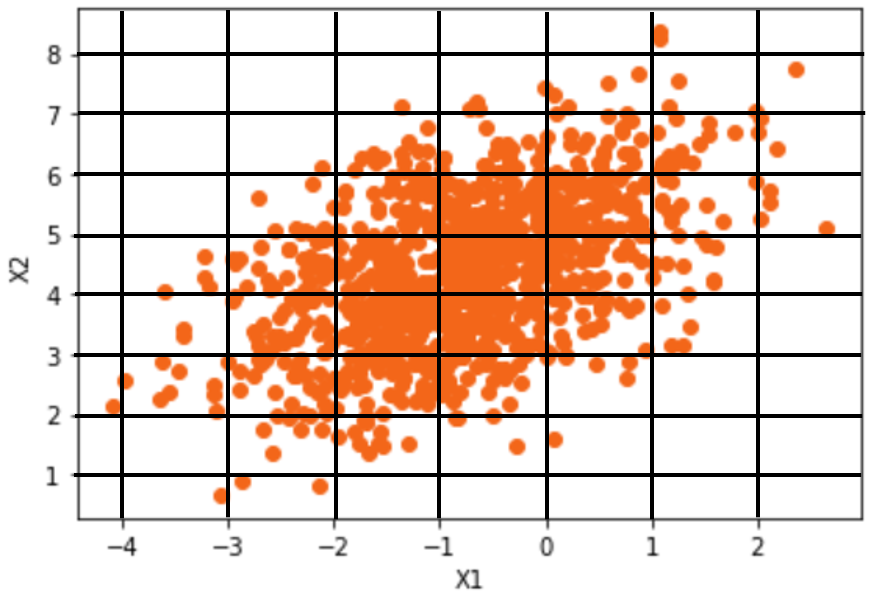
\includegraphics[width=0.6\textwidth]{discretization_uniform.png}
    \caption{Uniform discretization.}
    \label{figure:discretization_uniform}
\end{figure}

A better approach would be to compute the convex hull arund the actual cloud of points, and then divide the space into sqrt intervals of the same length, by for example, computing the n centroid using a kmeans algorithm and then useing voronoi pologons. Howerver, up to the best of our knowledge, a discretization algorithm based on a constrained version of the kmeans in which the distribution of the points is not changes, has not been developed.

\begin{figure}[ht]
    \centering
    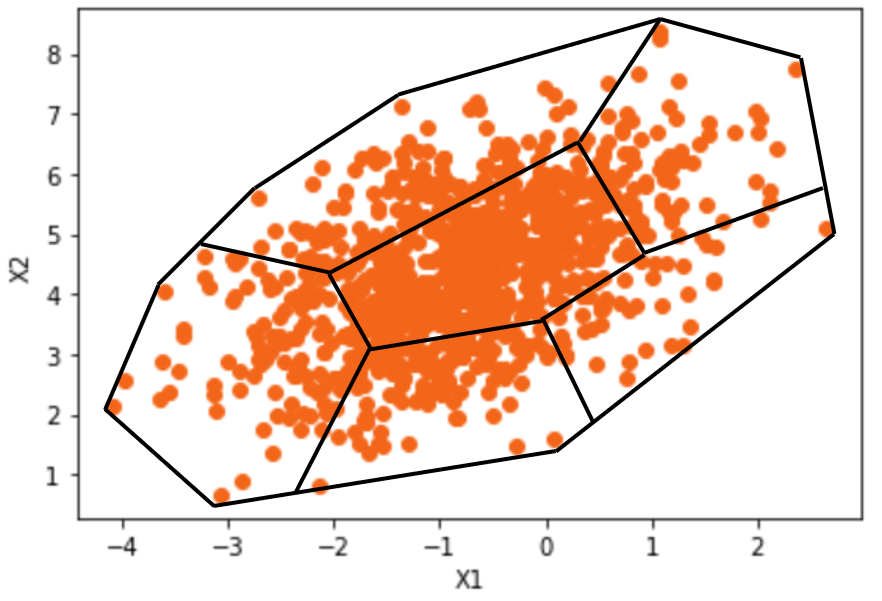
\includegraphics[width=0.6\textwidth]{discretization_kmeans.png}
    \caption{Convex hull and kmeans discretization.}
    \label{figure:discretization_kmeans}
\end{figure}


\end{remark}

%
% Section: Miscoding
%

\section{Miscoding}
\label{sec:machine_learning_miscoding}

In Section \ref{def:miscoding} we introduced the concept of miscoding as a quantitative measure of how well a string based encoding $r \in \mathcal{R}$ represents a research entity from $\mathcal{E}$. The miscoding of a representation $r$ was defined as:
\[
\mu(r) = \overset{o}{ \underset{s \in \mathcal{R}_\mathcal{E}} \min} \frac{ \max\{ K(s \mid r), K(r \mid s) \} } { \max\{ K(s), K(r) \} }
\]
and we saw that this quantity cannot be computed in practice for the general case. First of all because it requires a computation from an abstract oracle machine, second because it is based on the uncomputable Kolmogorov complexity, and third because it does not take into account the entity $e$ in which we are interested. 

In this section we are going to see how this concept can be adapted in practice to compute the error made by using a dataset $\mathbf{X}$ as a representation of a response variable $\mathbf{y}$ (see Section \ref{sec:machine_learning}). Our goal is double, in one hand we are interested in measuring the quality of the dataset $\mathbf{X}$ as a predictor of the variable $\mathbf{y}$, and in the other we want to identify those features $\mathbf{x}_j$ of $\mathbf{X}$ that have the higher predictive power for $\mathbf{y}$. This is the problem addressed by discriminative models (see Section \ref{sec:generative_discriminative}) in which we want to estimate the conditional distribution $P( \mathbf{y} \mid \mathbf{X} )$.

Given a training dataset $\mathbf{X}$, we can approximate the miscoding of a feature $\mathbf{x}_j$ for the target variable $\mathbf{y}$ by computing the normalized information distance between $\mathbf{x}_j$ and $\mathbf{y}$ (see Section \ref{sec:information_distance}):
\[
E(\mathbf{x}_j, \mathbf{y}) = \frac{\max\{ K(\mathbf{x}_j \mid \mathbf{y}), K(\mathbf{y} \mid \mathbf{x}_j) \}}{\max \{ K(\mathbf{x}_j), K(\mathbf{y}) \} }
\]
The Kolmogorov complexity $K(\mathbf{v})$ of a vector $\mathbf{v}$ will be approximated by the length of the compressed version of that vector $\hat{K}_C(\mathbf{v})$ using as compressor a minimal length code $C$ (see Section \ref{sec:note_about_compression}).

\begin{definition}
Let $\mathbf{y}$ be a response variable, $\mathbf{X}$ a dataset composed by $p$ features, and $\mathbf{x}_j$ the $j-th$ feature. We define the regular feature miscoding of $\mathbf{x}_j$ as a representation of $\mathbf{y}$, denoted by $\hat\mu(\mathbf{x}_j, \mathbf{y})$, as:
\[
\hat\mu(\mathbf{x}_j, \mathbf{y}) = \frac{ \hat{K}_C(\mathbf{x}_j, \mathbf{y}) - \min\{ \hat{K}_C(\mathbf{x}_j), \hat{K}_C(\mathbf{y}) \} } { \max\{ \hat{K}_C(\mathbf{x}_j), \hat{K}_C(\mathbf{y}) \} }
\]\end{definition}

Intuitively, the quantity $\hat\mu(\mathbf{x}_j, \mathbf{y})$ is a measure of the effort, as the length of a computer program and in relative terms, required to fully encode $\mathbf{y}$ assuming a knowledge of $\mathbf{x}_j$, and the other way around. The lower this value, the better would be the quality of $\mathbf{x}_j$ as a predictor for $\mathbf{y}$.

\begin{example}

Let's $\mathbf{y}$ be a target variable composed by $1.000$ random samples that follows a normal distribution $N(3,1)$ with mean $\mu = 3$ and standard deviation $\sigma = 1$, $\mathbf{x}_1$ be a predictor feature that is equal to $\mathbf{y}$ with some random noise, that is $\mathbf{x}_1 = \mathbf{y} + N(3, 1) / 10$, and $\mathbf{x}_2$ be a second predictor based on random samples from a exponential distribution with a rate of $\lambda = 1$.

\begin{sourcecode}
{\scriptsize \begin{verbatim}
from scipy.stats import norm, expon

y  = norm.rvs(loc=3, scale=1, size=10000)
x1 = y + norm.rvs(loc=3, scale=1, size=10000) / 10
x2 = expon.rvs(size=10000)
\end{verbatim}}
\end{sourcecode}

We can use the Nescience library to compute the miscoding of the features $\mathbf{x}_1$ and $\mathbf{x}_2$ when they encode the target variable $\mathbf{y}$.

\begin{sourcecode}
{\scriptsize \begin{verbatim}
from fastautoml.miscoding import Miscoding
import numpy as np

X = np.column_stack((x1, x2))

miscoding = Miscoding()
miscoding.fit(X, y)
miscoding.miscoding_features(mode="regular")
\end{verbatim}}
\end{sourcecode}

The output of the library would be something similar to the following\footnote{Since we are generating a list of $1.000$ random samples, the reader could get a slightly different result when running this example.}:

\begin{sourcecode}
{\scriptsize \begin{verbatim}
array([0.27445364, 0.9934222])
\end{verbatim}}
\end{sourcecode}

As it was expected the miscoding of $\hat\mu(\mathbf{x}_1, \mathbf{y})$ is much smaller than the miscoding of $\hat\mu(\mathbf{x}_2, \mathbf{y})$. In this case, we should prefer $\mathbf{x}_1$ over $\mathbf{x}_2$ as a predictor of $\mathbf{y}$.

\end{example}

Sometimes we will use the normalized version of the complements of the individual miscodings, that is $\frac{ 1 - \hat\mu(\mathbf{x}_i, \mathbf{y}) } { \sum_{i=j}^p 1 - \hat\mu(\mathbf{x}_j, \mathbf{y}) }$, instead of the regular ones $\hat\mu(\mathbf{x}_i, \mathbf{y})$, because they are easier to compare with other feature selection techniques, and because they have a visually appealing interpretation. We call this version of miscoding the \emph{adjusted} feature miscoding.

\begin{example}
\label{example:gaussian_blob_miscoding}
In this example we are going to generate a synthetic dataset where the target variable $\mathbf{y}$ is a collection of normally-distributed clusters of points, and the training set $\mathbb{X}$ is composed by both, relevant and irrelevant predictors. In particular we will generate $1.000$ samples composed by $20$ features that describe $10$ clusters; only $4$ of the features are relevant for prediction, and the other remaining $6$ are just random values.

In Figure \ref{figure:gaussian_blob_cluster} we can see a two-dimensional projection of this dataset, along the hyperplane composed by features 8 and 10.

\begin{figure}[h]
\centering
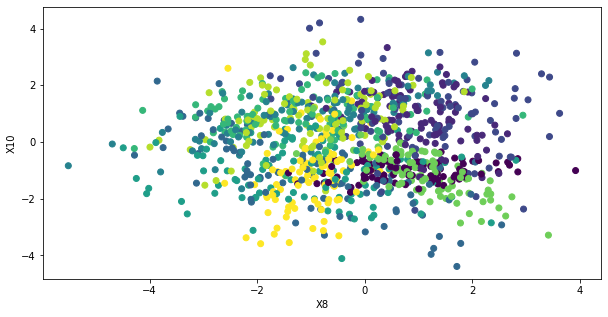
\includegraphics[width=0.6\textwidth]{gaussian_blob_cluster.png}
\caption{Gaussian Blob Cluster.}
\label{figure:gaussian_blob_cluster}
\end{figure}

\begin{sourcecode}
{\scriptsize \begin{verbatim}
from fastautoml.miscoding import Miscoding
from sklearn.datasets.samples_generator import make_classification

X, y = make_classification(n_samples=1000, n_features=20, n_informative=4,
       n_redundant=0, n_classes=10, n_clusters_per_class=1, flip_y=0)

miscoding = Miscoding()
miscoding.fit(X, y)
msd = miscoding.miscoding_features(mode='adjusted')
\end{verbatim}}
\end{sourcecode}

We will use the adjusted version of the miscoding for an easier comparison with other feature selection techniques. If we plot the results (see Figure \ref{figure:miscoding_make_classification}) we will see that the library has successfully identified the four relevant predictors ($\mathbf{x}_3$, $\mathbf{x}_8$, $\mathbf{x}_{10}$ and $\mathbf{x}_{16}$). Since we are using the adjusted version of miscodings, the higher the value the better, and mind that actual values have to be interpreted in relative terms. 

\begin{figure}[h]
\centering
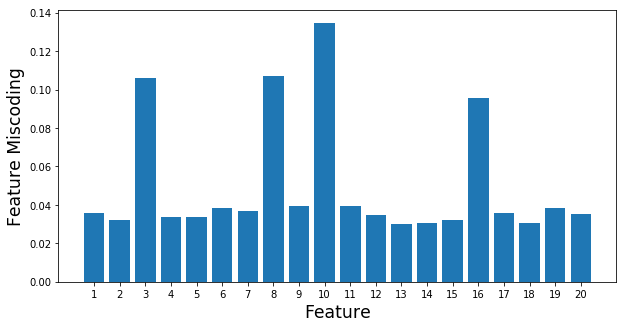
\includegraphics[width=0.6\textwidth]{feature_miscoding.png}
\caption{Miscoding of a Synthetic Dataset.}
\label{figure:miscoding_make_classification}
\end{figure}

We can compare miscoding with correlation, a common technique used in machine learning to identify the most relevant features of a dataset. In Figure \ref{figure:correlation_make_classification} is shown correlation between the individual features that compose $\mathbf{X}$ and the target variable $\mathbf{y}$. As we can observe, correlation fails to properly identify one of the relevant features ($\mathbf{x}_3$).

\begin{figure}[h]
\centering
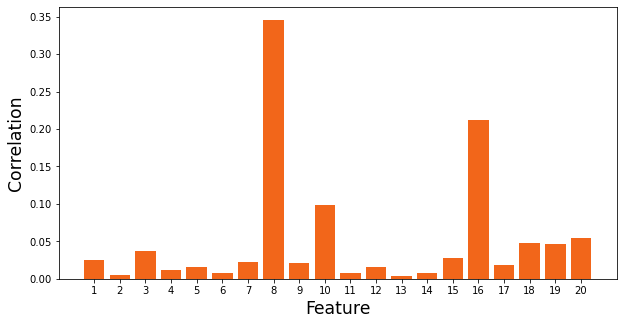
\includegraphics[width=0.6\textwidth]{feature_correlation.png}
\caption{Correlation of a Synthetic Dataset.}
\label{figure:correlation_make_classification}
\end{figure}

\end{example}

Feature miscoding allow us to identify the most relevant features of a training dataset $\mathbf{X}$, but it cannot be used to compute the miscoding of the dataset itself. If we start with a miscoding of $1$ (full unknown), and subtract the miscodings of the individual features, we will end up with a negative miscoding, something that it is not allowed by our theory. If we use the adjusted version, the dataset miscoding will be $0$ for all datasets, which is against our intuition that not all possible datasets $\mathbf{X}$ represent equally well a target variable $\mathbf{y}$. According to the theory of nescience, we expect that non-relevant features add, instead of subtract, to the global miscoding of the dataset.

In order to address this problem, we have to introduce the concept of partial miscoding of a feature, as the difference between the adjusted and normalized miscodings.

\begin{definition}
Let $\mathbf{y}$ be a target variable, $\mathbf{X}$ a dataset composed by $p$ features, and $\mathbf{x}_j$ the $j-th$ feature. We define the partial miscoding of $\mathbf{x}_j$ as a representation of $\mathbf{y}$, denoted by $\tilde\mu(\mathbf{x}_j, \mathbf{y})$, as:
\[
\tilde\mu(\mathbf{x}_i, \mathbf{y}) = \frac{ 1 - \hat\mu(\mathbf{x}_i, \mathbf{y}) } { \sum_{j=1}^p 1 - \hat\mu(\mathbf{x}_j, \mathbf{y}) } - \frac{\hat\mu(\mathbf{x}_i, \mathbf{y}) } { \sum_{j=1}^p \hat\mu(\mathbf{x}_j, \mathbf{y}) }
\]
\end{definition}

A positive partial miscoding means that the feature contributes to describe the target variable, meanwhile a negative value means that the feature is not relevant.

\begin{example}
\label{example:partial_feature_miscoding}
We will use again the synthetic dataset of Example \ref{example:gaussian_blob_miscoding}, but we will increase the number of relevant features from $4$ to $14$. Then, we will compute the list of partial miscodings.

\begin{sourcecode}
{\scriptsize \begin{verbatim}
from fastautoml.miscoding import Miscoding
from sklearn.datasets.samples_generator import make_classification

X, y = make_classification(n_samples=1000, n_features=20, n_informative=14,
       n_redundant=0, n_classes=10, n_clusters_per_class=1, flip_y=0)

miscoding = Miscoding()
miscoding.fit(X, y)
msd = miscoding.miscoding_features(mode="partial")
\end{verbatim}}
\end{sourcecode}

As we can see in Figure \ref{figure:partial_feature_miscoding}, not only the library has been able to correctly identify the relevant features, but also, non relevant features have now a negative contribution to the global miscoding.

\begin{figure}[h]
\centering
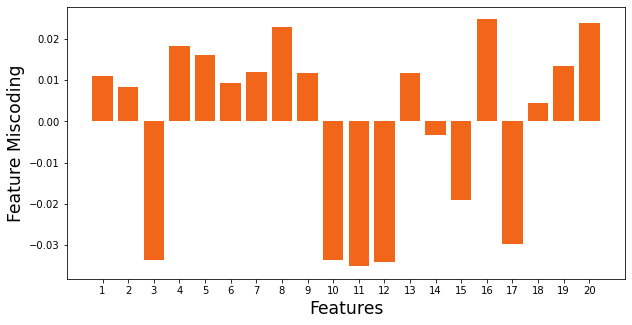
\includegraphics[width=0.6\textwidth]{partial_miscoding.png}
\caption{Partial Feature Miscoding.}
\label{figure:partial_feature_miscoding}
\end{figure}

\end{example}

Given the definition of partial feature miscoding we can provide a definition of the concept of miscoding of a target variable given a subset of predictors that it is closer to the original concept of miscoding defined by the theory of nescience.

\begin{definition}
Let $\mathbf{y}$ be a target variable, $\mathbf{X} = \{ \mathbf{x}_1, \ldots, \mathbf{x}_p \}$ a dataset composed by $p$ features, and $\mathbf{Z} = \{ \mathbf{z}_1, \ldots, \mathbf{z}_k \}$ a subset of features, that is, $\{ \mathbf{z}_1, \ldots, \mathbf{z}_k \} \subseteq \{ \mathbf{x}_1, \ldots, \mathbf{x}_p \}$. We define the miscoding of $\mathbf{Z}$ as a representation of $\mathbf{y}$, denoted by $\hat\mu(\mathbf{Z}, \mathbf{y})$, as:
\[
\hat\mu(\mathbf{Z}, \mathbf{y}) = \sum_{i=1}^k \tilde\mu (\mathbf{z}_i, \mathbf{y})
\]
\end{definition}

\begin{example}
\label{example:accumulated_partial_feature_miscoding}
Based on the dataset and the partial features miscoding computed in Example \ref{example:partial_feature_miscoding}, in Figure \ref{figure:accumulated_partial_feature_miscoding} we can see the evolution of the miscoding of the training subset $\mathbf{Z}$ as we add more features to the study.

\begin{figure}[h]
\centering
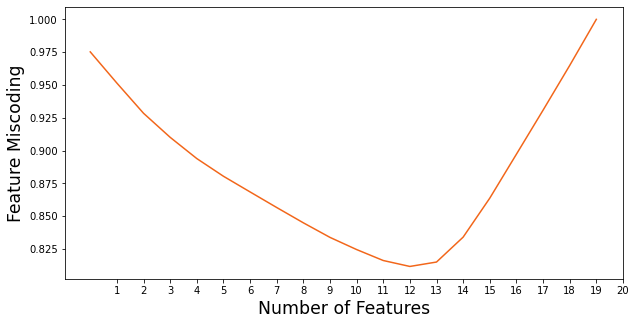
\includegraphics[width=0.6\textwidth]{accumulated_partial_miscoding.png}
\caption{Accumulated Partial Feature Miscoding.}
\label{figure:accumulated_partial_feature_miscoding}
\end{figure}

\end{example}

In the following example we are going to compare the performance of a machine learning classifier when using a full dataset and a reduced version of the same dataset using only those features identified as relevant, i.e., with positive partial miscoding.

\begin{example}
Let's train a neural network with the standard MNIST dataset in order to classify hand written digits. The evaluation criteria will be the score of the classifier, that is, the percentage of digits correctly classified, applied over a test dataset different from the dataset used for training. The neural network will be trained and evaluated using all the features that compose the dataset, and with a reduced version of the dataset composed by only those features with a positive partial miscoding.

\begin{sourcecode}
{\scriptsize \begin{verbatim}
import numpy  as np
from sklearn.model_selection import train_test_split
from sklearn.neural_network import MLPClassifier
from sklearn.datasets import load_digits
from fastautoml.fastautoml import Miscoding

data = load_digits()
X_raw = data.data
y_raw = data.target

miscoding = Miscoding()
miscoding.fit(X_raw, y_raw)
mscd = miscoding.miscoding_features(miscoding='partial')
X_red = X_raw[:,np.where(mscd > 0)[0]]
y_red = y_raw

X_raw_train, X_raw_test, y_raw_train, y_raw_test = train_test_split(X_raw,
             y_raw, test_size=.3)
X_red_train, X_red_test, y_red_train, y_red_test = train_test_split(X_red,
             y_red, test_size=.3)

clf = MLPClassifier(alpha=1, max_iter=1000)

clf.fit(X_raw_train, y_raw_train)
score_raw = clf.score(X_raw_test, y_raw_test)
        
clf.fit(X_red_train, y_red_train)
score_red = clf.score(X_red_test, y_red_test)
        
reduction = 1 - X_red_train.shape[1] / X_raw_train.shape[1]

print("Score raw:", score_raw, " Score Miscoding:", score_red,
      " Reduction:", reduction)

Score raw: 0.9833333333333333  Score Miscoding: 0.9814814814814815  Data Reduction: 0.46875
\end{verbatim}}
\end{sourcecode}

If we run the above source code, we will see that the score of the neural network classifier is about the same for the two datasets, 98\% of the digits are correctly classified using the test data. However, the reduced dataset used for training based on the optimal miscoding is 43\% smaller than the original dataset. This size reduction could have a big impact in the training time of the neural network. Smaller datasets are also relevant when working with ensembles of models, like random forests, where hundreds or thousands of models have to be trained.

\end{example}

Intuitively, as Example \ref{example:accumulated_partial_feature_miscoding} shows, we should prefer the subset $\mathbf{Z}$ of $\mathbf{X}$ composed by all those features whose partial miscoding are greater than zero. However, as we will see in the following sections of this chapter, this might not be the case. Feature selection is only one of the criteria used in the process of finding an optimal model for an entity represented by a dataset. It might happen that other elements, like inaccuracy or surfeit, suggest to use a different subset of predictors. The global optimization criteria we should use is the concept of nescience. A sensible approach to use partial miscoding would be to incrementally add to our model those features with higher miscoding, until all features with a positive value have been added, or an optimality criterion has been reached.

In case of having a generative model (see Section \ref{sec:generative_discriminative}), that is, a machine learning algorithm designed to find the joint probability $P(\mathbf{X}, \mathbf{y})$, we could use miscoding to compute how the different features relate to each other, that is, the quantity $\hat\mu(\mathbf{x}_i, \mathbf{x}_j)$ for each pair of values $i, j \leq p$. The result would be a miscoding matrix (see Example \ref{example:miscoding_boston}).

\begin{example}
\label{example:miscoding_boston}
The Boston dataset included in \texttt{scikit-learn} library contains a collection of variables that (potentially) could explain the price of houses in the area of Boston. In this example, instead of computing which are the factors that contribute the most to the price of houses, we are going to study the inter-dependence between these factors, using a miscoding matrix.

\begin{sourcecode}
{\scriptsize \begin{verbatim}
from fastautoml.fastautoml import Miscoding
from sklearn.datasets import load_boston

data = load_boston()

miscoding = Miscoding(X_type="numeric", y_type="numeric")
miscoding.fit(data.data, data.target)
mscd_matrix = miscoding.features_matrix(mode='regular')
\end{verbatim}}
\end{sourcecode}

In Figure \ref{figure:miscoding_matrix} we can see a graphical representation using a heatmap of the miscoding matrix computed over the features. The darker values represent a lower miscoding (mind we are using the regular version of the concept of miscoding). In particular, the values of the main diagonal are equal to zero. 

\begin{figure}[h]
\centering
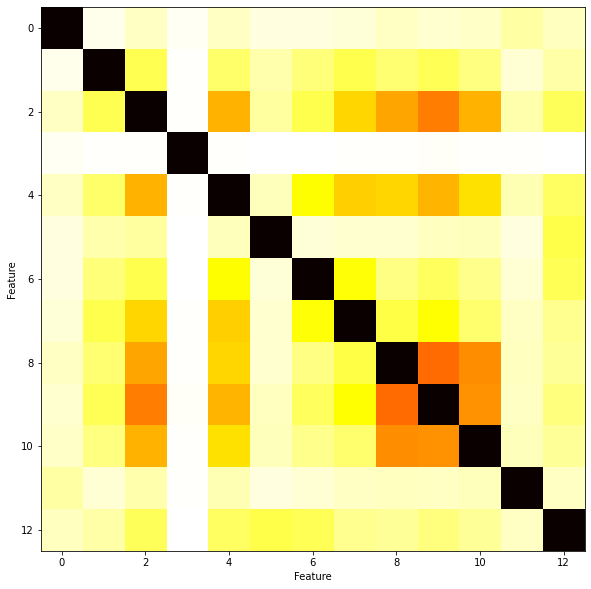
\includegraphics[width=0.4\textwidth]{miscoding_matrix.png}
\caption{Regular Miscoding Matrix.}
\label{figure:miscoding_matrix}
\end{figure}

The minimum value of $0.52$ is obtained with the pair $(8, 9)$ that correspond to the features "index of accessibility to radial highways" and "full-value property-tax rate per \$10,000". These features are good candidates to evaluate in a predictive model, since they contain non-redundant information. The maximum value of $0.99$ is achieved with the pair $(3, 12)$ with the features "Charles River dummy variable" and "\% lower status of the population". These features contains almost the same information, and so, including both in a model does not add nothing new, but increases the complexity of the model and the risk of over-fitting.

\end{example}

%
% Section: Inaccuracy
%

\section{Inaccuracy}
\label{sec:machine_learning_inaccuracy}

In Section \ref{sec:inaccuracy:inaccuracy} we defined the inaccuracy of a description $d \in \mathcal{D}$ for a representation $r \in \mathcal{R}$ as the normalized information distance between the representation $r$ and the string $\Gamma(d)$ printed out by a universal Turing machine when given the description as input:
\[
\iota(d, r) = \frac{ \max\{ K \left(r \mid \Gamma(d) \right), K \left( \Gamma(d) \mid r \right) \} } { \max\{ K(r), K \left(\Gamma(d) \right) \} }
\]

Inaccuracy, being based in Kolmogorov complexity, is not computable for the general case, and so, it has to be approximated in practice. In this section we are going to see how this concept can be estimated in case of a model trained using a dataset. The approach will be similar to the one used in case of miscoding (see Section \ref{sec:approx-miscoding} for more information).




{\color{red} TODO: This definition correspond to the discriminative case. Introduce the generative case as well.}

\begin{definition}
Let $\mathbb{X}$ be a dataset, $\mathbf{y}$ a response variable, $m$ a model, and $\mathbf{\hat{y}} = m(\mathbb{X})$ the predicted values by $m$ given $\mathbb{X}$. We define the \emph{inaccuracy}\index{Inaccuracy} of the model $m$ for the target values $\mathbf{y}$, denoted by $\hat\iota(\mathbf{\hat{y}}, \mathbf{y})$, as:
\[
\hat\iota(\mathbf{\hat{y}}, \mathbf{y}) = \frac{ \hat{K}_C(\mathbf{\hat{y}}, \mathbf{y}) - \min\{ \hat{K}_C(\mathbf{\hat{y}}), \hat{K}_C(\mathbf{y}) \} } { \max\{ \hat{K}_C(\mathbf{\hat{y}}), \hat{K}_C(\mathbf{y}) \} }
\]\end{definition}

Intuitively, the quantity $\hat\iota(\mathbf{\hat{y}}, \mathbf{y})$ is a measure of how far are the predicted values from real values. The lower this quantity, the better is the quality of $m$ as a predictor for $\mathbf{y}$. With our new inaccuracy metric we are measuring not only how difficult is to reconstruct the original target vector $\mathbf{y}$ given the predicted values $\mathbf{\hat{y}}$, but also how much additional information $\mathbf{\hat{y}}$ contains that is not related to $\mathbf{y}$, being the latter a novelty with respect to other metrics used in machine learning to measure the accuracy of a model.

\begin{example}
\label{ex:machine_learning:inaccuracy:inaccuracy_DT}
Inaccuracy, according to the minimum nescience principle, is given by the normalized compression distance between the actual targets $\mathbf{y}$ and the predicted targets $\mathbf{\hat{y}}$ by the model. In the following example we are going to compare the behavior of our new inaccuracy metric with a classical score metric. The experiment will be based on the MNIST\index{MNIST} dataset (hand written digits recognition) provided by scikit-learn.

\begin{sourcecode}
{\scriptsize \begin{verbatim}
from fastautoml.fastautoml import Inaccuracy
from sklearn.datasets import load_digits

X, y = load_digits(return_X_y=True)

inacc = Inaccuracy()
inacc.fit(X, y)
\end{verbatim}}
\end{sourcecode}

For this example we will train a decision tree classifier up to a pre-determined tree depth of $i$, where $i$ goes from $1$ to $20$.

\begin{sourcecode}
{\scriptsize \begin{verbatim}
from sklearn.tree import DecisionTreeClassifier

scores       = list()
inaccuracies = list()

for i in range(20):
    
    tree = DecisionTreeClassifier(max_depth=i, random_state=42)
    tree.fit(X, y)
    
    scores.append(1 - tree.score(X, y))
    inaccuracies.append(inacc.inaccuracy_model(tree))
\end{verbatim}}
\end{sourcecode}

We are interested to compare the behavior of score (actually we are comparing against one minus score) and inaccuracy metrics. As we can see in Figure \ref{figure:machine_learning:inaccuracy:inaccuracy_DT}, both metrics present a similar behavior, having inaccuracy a larger value, due to a stronger emphasis in incorrectly predicted values.

\begin{figure}[h]
\centering
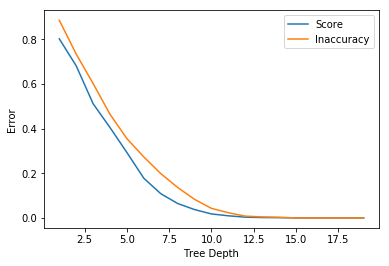
\includegraphics[width=0.6\textwidth]{inaccuracy_DT.png}
\caption{Inaccuracy vs. Score of Decison Trees}
\label{figure:machine_learning:inaccuracy:inaccuracy_DT}
\end{figure}

\end{example}

In Example \ref{ex:machine_learning:inaccuracy:inaccuracy_DT} we have seen that the deeper the tree, the smaller is the training error. Of course, the higher the value of $i$, the higher the risk of overfitting\index{Overfitting} the data. However, in case of inaccuracy we are not interested in avoiding overfitting, since overfitting is controlled by the metric of surfeit (see Section \ref{sec:machine_learning:surfeit}).

We can see inaccuracy as the effort, measured as the length of a computer program, required to fix the predictions made by a model. In this sense, according to the minimum nescience principle, it is not the same a model that makes one hundred times the same error than a model that makes one hundred different errors, since it should be easier to fix the former than the later (see Example \ref{ex:machine_learning:inaccuracy:one_hundred_errors}).

\begin{example}
\label{ex:machine_learning:inaccuracy:one_hundred_errors}
In this example we are going to use again a decision tree classifier, but this time it will be trained with the hyperparameter minimum number of samples per leaf node set to 5 (a common approach used in practice to avoid decision trees to overfit).

\begin{sourcecode}
{\scriptsize \begin{verbatim}
tree = DecisionTreeClassifier(min_samples_leaf=5)
tree.fit(X, y)
\end{verbatim}}
\end{sourcecode}

The inaccuracy of this new trained model is $0.17$, and its score $0.08$. Next we will artificially introduce one hundred errors in the dataset, simulating the case that the tree is not able to model correctly these data points. In this particular case all the errors are exactly the same.

\begin{sourcecode}
{\scriptsize \begin{verbatim}
X2 = X.copy()
y2 = y.copy()
for i in range(100):
    X2 = np.append(X2, [X[0]], axis=0)
    y2 = np.append(y2, (y[0]+1) % 10)
\end{verbatim}}
\end{sourcecode}

The inaccuracy of the decision tree, given this new dataset, has increased\footnote{Note that we had to \texttt{fit()} again the class Inaccuracy in order to use the new dataset. Normally this is not the way we use this class; instead what we should do is to fit once a dataset, and then compute the inaccuracy of different models. We are doing here in this way to demonstrate an interesting property of the concept of inaccuracy.} from $0.17$ to $0.21$.

\begin{sourcecode}
{\scriptsize \begin{verbatim}
inacc.fit(X2, y2)
inacc.inaccuracy_predictions(pred)
\end{verbatim}}
\end{sourcecode}

Score has also increased, in this case from $0.08$ to $0.13$.

\begin{sourcecode}
{\scriptsize \begin{verbatim}
1 - tree.score(X2, y2)
\end{verbatim}}
\end{sourcecode}

Finally, we are going to repeat exactly the same experiment, but this time instead of adding one hundred times the same error, adding one hundred different errors.

\begin{sourcecode}
{\scriptsize \begin{verbatim}
X3 = X.copy()
y3 = y.copy()
for i in arange(100):
    index = np.random.randint(X.shape[0])
    X3    = np.append(X3, [X[index]], axis=0)
    y3    = np.append(y3, (y[index]+1) % 10)
\end{verbatim}}
\end{sourcecode}

In this last case the inaccuracy of the model has increased up to $0.25$, meanwhile score remained the same.
\end{example}

In line with Example \ref{ex:machine_learning:inaccuracy:one_hundred_errors}, an extreme case would be a model for a target binary variable (True and False) that always fails with its predictions, that is, if the value of the target is True, the model will predict False, and if it is False, it will predict True. The classical evaluation metrics would say that this model is the worst possible model, but our inaccuracy would claim that the model is perfect. We might be wondering what it is the value of a model that always fails to predict the correct target. But if we are the managers of an edge fund investing in the stock market\index{Stock market}, we will very happy to pay a huge amount of money for a model that predicts that the shares of IBM will go down whenever they go up, and the other way around.

In case of having a highly unbalanced dataset\index{Unbalance dataset}, that is, when some categories have a lot of more training data than others, the classical score metric can provide a misleading result, since a good score does not necessarily mean a good model, it might happen that the model is simply properly classifying the samples of the category with the higher number of training samples, and misclassifying the others. In practice, we solve this problem by using metrics specifically designed to deal with unbalanced datasets. In case of the new metric of inaccuracy, as Example \ref{ex:machine_learning:inaccuracy:unbalanced_dataset} shows, a model that can not properly classify one of the categories is considered a bad model, even if this category has only a few points in the training dataset.

\begin{example}
\label{ex:machine_learning:inaccuracy:unbalanced_dataset}
For this example, we will create a synthetic dataset using the \texttt{make\_classification} utility of scikit-learn, with two classes in which one of then has 95\% of the samples, and the other 5\%.

\begin{sourcecode}
{\scriptsize \begin{verbatim}
from sklearn.datasets import make_classification

depth = list()
score = list()
inacc = list()

inaccuracy = Inaccuracy()

for i in np.arange(1, 100):
                    
    X, y = make_classification(n_samples=1000, n_features=2,
                               n_informative=2, n_redundant=0,
                               class_sep=2, flip_y=0, weights=[0.95,0.05])

    inaccuracy.fit(X, y)
        
    tree = DecisionTreeClassifier(min_samples_leaf=i)
    tree.fit(X, y)

    depth.append(i)        
    score.append(1 - tree.score(X, y))
    inacc.append(inaccuracy.inaccuracy_model(tree))
\end{verbatim}}
\end{sourcecode}

The experiment consists in training a decision tree classifier with a minimum number of samples per leaf of $i$, where $i$ goes from 1 to 100. In Figure \ref{figure:machine_learning:inaccuracy:inaccuracy_DT2} we can see the behavior of inaccuracy and score. In case of large values of $i$, the score metric tell us that no more than a 5\% of the samples is misclassified, however, the inaccuracy says that even if the total number of misclassified points is low, the inaccuracy of the model is very bad.

\begin{figure}[h]
\centering
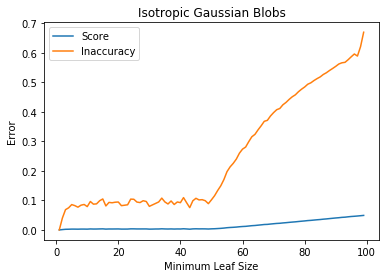
\includegraphics[width=0.6\textwidth]{inaccuracy_DT2.png}
\caption{Inaccuracy of Decision Tree.}
\label{figure:machine_learning:inaccuracy:inaccuracy_DT2}
\end{figure}

\end{example}





%
% Section: Surfeit
%

\section{Surfeit}
\label{sec:machine_learning_surfeit}

In Section \ref{sec:Definition_redundancy} we defined the surfeit of the model $m \in \mathcal{M}$ for the representation $r \in \mathcal{R}$ as:
\[
\sigma (m, r) = 1 - \frac{K(r)}{l(m)}
\]
Since the length $K(r)$ of shortest possible model for the representation $r$ is in general unknown, we have to approximate this concept in practice. In case of having a training dataset $\mathbb{X}$ and a target variable $\mathbf{y}$, we can approximate the surfeit of a model $m$ for the representation $\mathbf{y}$ by means of computing:
\[
\hat\sigma(m, y) = 1 - \frac{\hat{K}_C(\mathbf{y})}{l(m)}
\]
Where $\hat{K}_C(\mathbf{y})$ is the length of the compressed version of the of the vector $\mathbf{y}$ using as compressor a minimal length code $C$, computed given the relative frequencies of the values observed in $\mathbf{y}$ (see Section \ref{sec:approx-miscoding}).

\begin{definition}
Let $\mathbf{y}$ be a response variable, $\mathbb{X}$ a dataset composed by $p$ features and $n$ samples. We define the surfeit of the model $m \in \mathcal{M}$ as a representation of $\mathbf{y}$, denoted by $\hat\sigma(m, \mathbf{y})$, as:
\[
\hat\sigma(m, \mathbf{y}) = 1 - \frac{\hat{K}_C(\mathbf{y})}{l(m)}
\]
\end{definition}

The definition of surfeit requires a method of encoding the models as a string of symbols, so we can compute their length. Ideally, we should use as encodings Turing machines, and agree upon an universal Turing machine to interpret those models. However, that would make very difficult to add new models to the nescience library. Instead, we have used for the encoding of models a simplified version of the Python language, where not all the constructions are allowed, and we do not allow the use of libraries.

Surfeit is a metric that can help us to avoid overfitted models. The higher is the surfeit of a model, the higher is the probability that the model is an overfit of the training dataset, as Example \ref{ex:surfeit_overfit} shows.

\begin{example}
\label{ex:surfeit_overfit}
In this example we are going to generate a dataset composed by $900$ samples of a sinusoidal curve, and we will fit the data using a $n$ degree polynomial, where $n$ goes form $1$ to $15$.

\begin{sourcecode}
{\scriptsize \begin{verbatim}
from sklearn.linear_model import LinearRegression
from sklearn.preprocessing import PolynomialFeatures

from Nescience.Nescience import Surfeit
from Nescience.Nescience import Inaccuracy

n_samples = 900
degrees = np.arange(1, 15)

X = np.sort(np.random.rand(n_samples) * 3)
y = np.cos(1.5 * np.pi * X)

linacc   = list()
lsurfeit = list()

for i in degrees:
        
    poly = PolynomialFeatures(degree=i, include_bias=False)
    newX = poly.fit_transform(X[:, np.newaxis])
    
    linear_regression = LinearRegression()
    linear_regression.fit(newX, y)

    inacc.fit(newX, y)
    inaccuracy = inacc.inaccuracy_model(linear_regression)
    
    sft.fit(newX, y)
    surfeit = sft.surfeit_model(linear_regression)
    
    linacc.append(inaccuracy)
    lsurfeit.append(surfeit)
\end{verbatim}}
\end{sourcecode}

In figure \ref{figure:surfeit_vs_inaccuracy} we can see the results of this experiment. As it was expected, the higher the degree of the polynomial, the smaller is the error of the model. However, at the same time we see that the higher the polynomial, the higher the surfeit of the model. The ideal model is that one that has a low inaccuracy and a low surfeit.

\begin{figure}[h]
\centering
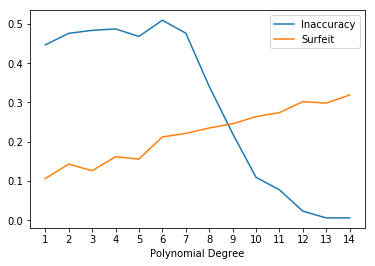
\includegraphics[width=0.6\textwidth]{surfeit_vs_inaccuracy.png}
\caption{Surfeit vs Inaccuracy}
\label{figure:surfeit_vs_inaccuracy}
\end{figure}

\end{example}

Another advantage of the concept of surfeit is that it allows us to compare and decide between models that belong to different families. For example, in case of models having the same accuracy, shall we prefer a decision tree over a neural network, or a naive Bayes classifier over a support vector machine? Next example shows how we can decide about those questions.

\begin{example}
\label{ex:dt_vs_nn}

In this example we are going to compare a decision tree with a neural network. We will use a synthetic dataset composed by two isotropic Gaussian blobs, and we will train our models to split them apart. In the first part of the example we will use a standard deviation of $1$ and only two dimensions, so the two clusters are easy to classify (see figure on Table \ref{tab:isotropic_gaussian_blobs}, left side).

\begin{table}
\begin{center}

\begin{tabular}{ c c }

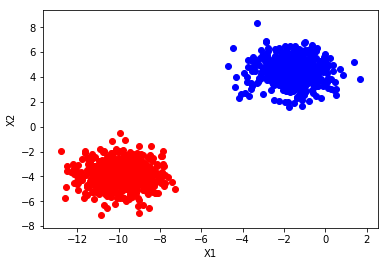
\includegraphics[scale=0.4]{blobs_easy_split} & 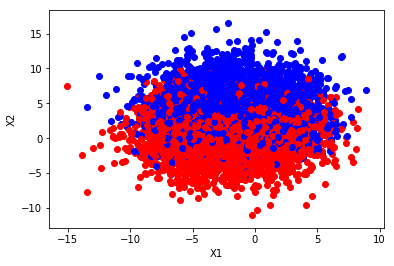
\includegraphics[scale=0.4]{blobs_difficult_split}

\end{tabular}
\end{center}
\caption{\label{tab:isotropic_gaussian_blobs}Isotropic Gaussian blobs.}
\end{table}

% \raisebox{.4\height}{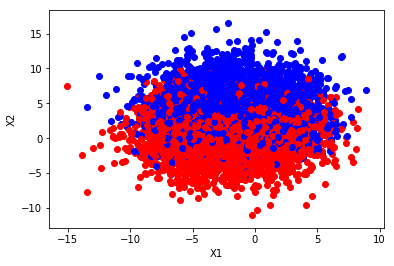
\includegraphics[scale=0.4]{blobs_difficult_split}}

\begin{sourcecode}
{\scriptsize \begin{verbatim}
from sklearn.tree import DecisionTreeClassifier
from sklearn.neural_network import MLPClassifier
from Nescience.Nescience import Surfeit
from Nescience.Nescience import Inaccuracy
from sklearn.datasets.samples_generator import make_blobs

X, y = make_blobs(n_samples=1000, centers=2, n_features=2, cluster_std=1)

tree = DecisionTreeClassifier()
tree.fit(X, y)
tree.score(X, y)

nn = MLPClassifier()
nn.fit(X, y)
nn.score(X, y)

sft = Surfeit()
sft.fit(X, y)

sft.surfeit_model(tree)
sft.surfeit_model(nn)

\end{verbatim}}
\end{sourcecode}

If we ran the above code we will see that both models have exactly the same accuracy of $1$, that is, they are perfect classifiers. However the surfeit of the decision tree is $0.25$, meanwhile the surfeit of the neural network is $0.73$. In this particular case we should prefer the decision tree over the neural network.

If we perform the same experiment using a standard deviation of $3$, so two clusters that are more difficult to split (see Table \ref{tab:isotropic_gaussian_blobs}, right side), the situation will change.

\begin{sourcecode}
{\scriptsize \begin{verbatim}
X, y = make_blobs(n_samples=10000, centers=2, n_features=8, cluster_std=3)
\end{verbatim}}
\end{sourcecode}

In this second case, again, both models have the same accuracy (we have increased the number of samples, and the number of dimensions, so the models can still perform a perfect classification), but the surfeit of the decision tree has increased to $0.82$, and the surfeit of the neural network is almost the same, $0.76$. For this second dataset we should prefer the neural network over the decision tree.

\end{example}

In example \ref{ex:dt_vs_nn} we have assumed that both models, decision tree and neural networks, have the same accuracy. When this is not the case, when the models do not have the same accuracy, we have to apply to the concept of nescience in order to decide between them. 

\begin{remark}
{\color{red} TODO: Mention the problem of the stability of the signal.}
\end{remark}

%
% Section: Nescience
%

\section{Nescience}
\label{sec:machine_learning_nescience}

In Chapter \ref{chap:Nescience} we defined the concept of nescience as the solution to a non-linear multi-objective optimization problem, where we had to minimize the miscoding, inaccuracy and surfeit of representations and models. The solution to this problem is, in general, not unique, in the sense that we can find multiple pairs of representations and models that have the property that we can not improve one of these quantities without degrading the others (Pareto optimality). However, in practice, we expect that a machine learning library should provide a single solution when training a model over a dataset. In order to provide this unique solution, we have to resort to a utility function that selects one from the available solutions. The nescience library provide different alternatives of utility functions, being the default one the arithmetic mean the tree metrics.

\begin{remark}
The nescience library implements the following utility functions to approximate the concept of nescience, that is, to compute $\hat\nu\left(\mathbb{Z}, m, \mathbf{y} \right)$:

\begin{itemize}
\item Euclid distance: $\left( \hat\mu(\mathbb{Z}, \mathbf{y})^2 + \hat\iota(\hat{y}, \mathbf{y})^2  + \hat\sigma(m, \mathbf{y})^2 \right)^{1/2}$
\item Arithmetic mean: $\frac{\hat\mu(\mathbb{Z}, \mathbf{y}) + \hat\iota(\hat{y}, \mathbf{y}) + \hat\sigma(m, \mathbf{y})}{3}$
\item Geometric mean: $\left( \hat\mu(\mathbb{Z}, \mathbf{y}) \times \hat\iota(\hat{y}, \mathbf{y}) \times \hat\sigma(m, \mathbf{y}) \right)^{1/3}$
\item Product: $\hat\mu(\mathbb{Z}, \mathbf{y}) \times \hat\iota(\hat{y}, \mathbf{y}) \times \hat\sigma(m, \mathbf{y})$
\item Addition: $\hat\mu(\mathbb{Z}, \mathbf{y}) + \hat\iota(\hat{y}, \mathbf{y}) + \hat\sigma(m, \mathbf{y})$
\item Weighted mean: $w_\mu \hat\mu(\mathbb{Z}, \mathbf{y}) + w_\iota \hat\iota(\hat{y}, \mathbf{y}) + w_\sigma \hat\sigma(m, \mathbf{y})$
\item Harmonic mean: $\frac{3}{ \hat\mu(\mathbb{Z}, \mathbf{y})^{-1} + \hat\iota(\hat{y}, \mathbf{y})^{-1} + \hat\sigma(m, \mathbf{y})^{-1} }$
\end{itemize}

Euclid distance and addition have the drawback that they produce nescience values greater than one, something that it is against our theory. Geometric mean, product and harmonic mean have the problem that the nescience is zero, or not defined, if one of the three metrics (miscoding, inaccuracy or surfeit) is zero. And the weighted mean introduce three new hyperparameters that have to be optimized. It is still an open question which one is the best utility function to compute the nescience of a dataset and a model.
\end{remark}

Example \ref{ex:nescience_decisiontree} shows how we can use the \texttt{nescience} library to compute the nescience of a dataset and a model.

\begin{example}
\label{ex:nescience_decisiontree}

This example shows how to compute in practice the nescience of a dataset and a model. In particular, we are going to compute the nescience of a decision tree classifier applied over the dataset digits (MNIST hand written digits classification problem) included in the \texttt{sklearn} library.

\begin{sourcecode}
{\scriptsize \begin{verbatim}
from sklearn.tree import DecisionTreeClassifier
from sklearn.datasets import load_digits
from Nescience.Nescience import Nescience

data = load_digits()

tree = DecisionTreeClassifier()
tree.fit(data.data, data.target)
tree.score(data.data, data.target
[ ] 1

nescience = Nescience()
nescience.fit(data.data, data.target)

nescience.nescience(tree)
[ ] 0.5895603819965907
\end{verbatim}}
\end{sourcecode}

The score of the decision tree model is $1$, meaning that all the samples have been properly classified. Of course, what happened is that the decision tree is overfitting the dataset. In order to avoid this kind of problems we usually split the data in separate training and testing subsets, or we perform a more advanced cross-validation. However, if we compute the nescience, we will get a value of $0.59$, rising the flag that something is wrong with the model or the training dataset.

\end{example}

In Example \ref{ex:nescience_decisiontree} we have shown that one of the advantages of the concept of nescience is that we can evaluate the quality of a model without applying computationally expensive procedures like cross-validation, and without requiring to save part of the data as a test subset. Another advantage of the metric nescience is that it allows us to decide between competing models from different families of models, as it is shown in Example \ref{ex:nescience_comparison}.

\begin{example}
\label{ex:nescience_comparison}

In this example we are going to compare two models from two different families of models: decision trees and neural networks. Both models will be trained with the breast cancer dataset provided by the \texttt{sklearn} library.

\begin{sourcecode}
{\scriptsize \begin{verbatim}
from sklearn.tree import DecisionTreeClassifier
from sklearn.neural_network import MLPClassifier
from sklearn.datasets import load_breast_cancer
from Nescience.Nescience import Nescience

data = load_breast_cancer()
X = data.data
y = data.target

tree = DecisionTreeClassifier(max_depth=3)
tree.fit(X, y)
tree.score(X, y)
[ ] 0.9789103690685413

nescience = Nescience()
nescience.fit(X, y)
nescience.nescience(tree)
[ ] 0.5945936419010083

nn = MLPClassifier()
nn.fit(X, y)
nn.score(X, y)
[ ] 0.9261862917398945

nescience.nescience(nn)
[ ] 0.7860523786210711
\end{verbatim}}
\end{sourcecode}

Both models have a similar score. In this case, not only the decision tree provide a better score, but also, the nescience is much lower than in case of the multi-layer perceptron, and so, we should prefer the former over the later.

\end{example}

Nescience is a metric that can be used to optimize the hyperparameters that define a (parametric) family of models. The advantage of nescience is that we can use a greeedy approach to select the best value for an hypeparameter, saving a lot of computational time and resources during the search. That is, if we have a model controlled by an hyperparameter such that the higher the value the better the score, we should select that value in which the nescience stops decreasing and starts to increase, since this is the point in which we are not longer learning anything new from that dataset (see Example \ref{ex:nescence_hyperparameter}).

\begin{example}
\label{ex:nescence_hyperparameter}

For this example we will use again a decision tree classifier with the breast cancer dataset. We will train $10$ different trees, setting the hyperparameter \texttt{max\_depth} with values from $1$ to $10$. The \texttt{max\_depth} hyperparameter controls how deep we allow the tree to grow in order to classify the samples of the dataset. The deeper the tree the higher the score of the model, but also, the higher the risk of overfitting the training data. For each tree we will compute the nescience of the model, and we will compare it with a cross validation score. The results are shown in Figure \ref{figure:nescience_cancer}. As we can see in the figure, both, nescience and cross validation score, decrease are we increase the depth of the tree, until we reach a point in which it starts to increase. This inflection point is where the model begins to overfit the data. The nescience library suggests to use a tree with a maximum depth of $7$, meanwhile with the cross validation we got an optimal level of 6.

\begin{figure}[h]
\centering
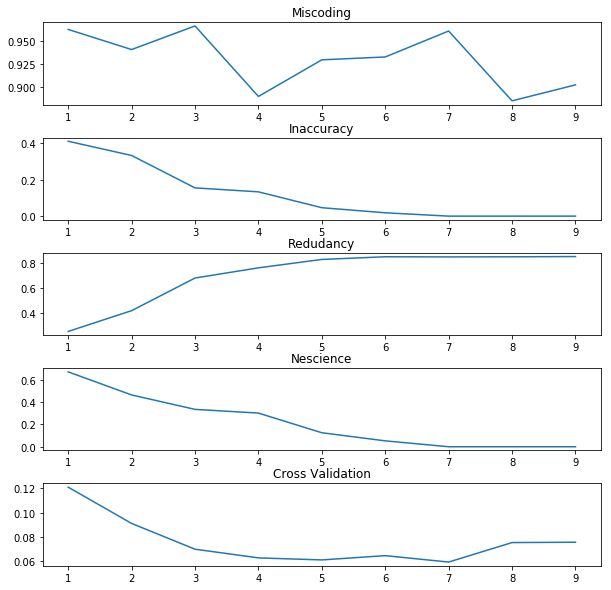
\includegraphics[width=0.6\textwidth]{nescience_cancer.png}
\caption{Evolution of Nescience with Tree Depth.}
\label{figure:nescience_cancer}
\end{figure}

\end{example}

It is interesting to note the behavior of the three metrics that define the concept of nescience in Figure \ref{figure:nescience_cancer}. As it is expected the the deeper the tree the smaller is the inaccuracy of the model and the higher the surfeit. However, in case of miscoding, we have a sort of random evolution. This behavior is due to the fact that each candidate tree uses a different subset of features at the decision nodes. I would be very nice to have an decision tree building algorithm that takes into account miscoding in order to decide the best features for new branches. Such an algorithm is described in Section \ref{sec:decision_trees}.

Finally, we are going to see how to use nescience in case of hyperparameter searches where we cannot apply a greedy approach, for example when the search is performed over a collection of (usually conflicting) hyperparameters. Hyperparameter search is a computationally expensive approach, since the number of possible combinations to test could be very large. Moreover, if for each candidate set we have to cross-validate the result, the search becomes prohibitive. As we have seen, nescience do not requires the use of crossvalidation to detect a situation of overfiting, and so, it can significantly speed up the process of searching for optimal hyperparameters. In Example \ref{ex:hyper_search} it is show how we can do that with the \texttt{nescience} library.

\begin{example}
\label{ex:hyper_search}

In this example we are going to see how we can use the \texttt{nescience} library to find the optimal hyperparameters for a model using a grid search. In particular, we are going to select the best hyperparameters for a multilayer perceptron classifer, including the number of hidden layers, and the size of those layers (what it is called Neural Architecture Search). The procedure will be demonstrated using the \texttt{digits} dataset.

\begin{sourcecode}
{\scriptsize \begin{verbatim}
from Nescience.Nescience import Nescience
from sklearn.neural_network import MLPClassifier
from sklearn.model_selection import GridSearchCV
from sklearn.metrics import classification_report
from sklearn.model_selection import train_test_split
\end{verbatim}}
\end{sourcecode}

First of all we have to provide a custom loss function based on the concept of nescience to be integrated with the search procedure. The next code shows how to implement such a function.

\begin{sourcecode}
{\scriptsize \begin{verbatim}
def my_custom_loss_func(estimator, X, y):
    
    nsc = Nescience()
    nsc.fit(X, y)
    nescience = nsc.nescience(estimator)
    
    # scikit-learn expect that higher numbers are better
    score = -nescience
    
    return score
\end{verbatim}}
\end{sourcecode}

Second, we have to define the grid of hyperparameters over which we are going to do the search. The larger the grid, the better the result, but also, the more computer time is required to evaluate all possible combinations.

\begin{sourcecode}
{\scriptsize \begin{verbatim}
parameters = {'solver': ['lbfgs'],
              'max_iter': [1000, 1500, 2000 ], 
              'alpha': 10.0 ** -np.arange(1, 10, 3),
              'hidden_layer_sizes':[(60,), (100,), (60, 60,), (100, 100,), 
                                    (60, 60, 60,), (100, 100, 100,)]}
\end{verbatim}}
\end{sourcecode}

Next code show how to do a classical grid search using the score of the models. The search will be evaluated using a train/test split of the dataset.
 
\begin{sourcecode}
{\scriptsize \begin{verbatim}
clf_std = GridSearchCV(estimator=MLPClassifier(), param_grid=parameters,
                       cv=3, iid=True, n_jobs=-1)
clf_std.fit(X_train, y_train)
clf_std.best_params_

[] {'alpha': 0.1,
[]  'hidden_layer_sizes': (100,),
[]  'max_iter': 1000,
[]  'solver': 'lbfgs'}

y_true, y_pred = y_test, clf_std.predict(X_test)
print(classification_report(y_true, y_pred))

[] precision    recall  f1-score   support
[] avg / total       0.98      0.97      0.97       540
\end{verbatim}}
\end{sourcecode}

Next code show how to perform exactly the same search, but using the concept of nescience instead of the metric score.

\begin{sourcecode}
{\scriptsize \begin{verbatim}
clf_nsc = GridSearchCV(estimator=MLPClassifier(), param_grid=parameters,
                       cv=3, scoring=my_custom_loss_func, iid=True)
clf_nsc.fit(X_train, y_train)
clf_nsc.best_params_

{'alpha': 0.1,
 'hidden_layer_sizes': (60,),
 'max_iter': 1500,
 'solver': 'lbfgs'}

y_true, y_pred = y_test, clf_nsc.predict(X_test)
print(classification_report(y_true, y_pred))

                  precision    recall    f1-score    support
avg / total       0.98         0.98      0.98        540
\end{verbatim}}
\end{sourcecode}

As we can see, the results provided by the \texttt{nescience} library are slightly better in terms of train/test evaluations. However, what it is important is the library has opted for a smaller model (one layer of $60$ neurons instead of one layer of $100$ neurons) that provides a better result by increasing the maximum number of iterations (from $1000$ to $1500$). Nescience always select the smallest model that provides the best possible accuracy that does not overfit the training data.

\end{example}

%
% Section: Auto Classification
%

\section{Auto Machine Classification}
\label{sec:machine_learning_classification}

The nescience library also includes a module for auto-machine learning (both for classification and regression problems). The auto-machine learning module returns the model, from a collection of families of models, that provides the smalles nescience. For each family of models, the class perform a greedy search over the hyperparameters required for each family. In Appendix XX is described the detail for each family of models.

Next example shows how to apply the automachine learning tools.

\begin{example}
\label{ex:automl}

In this example we are going to see how to apply the nescience library to find the best model that describes the \texttt{digits} dataset.

\begin{sourcecode}
{\scriptsize \begin{verbatim}
from sklearn.datasets import load_digits
from sklearn.model_selection import train_test_split

from Nescience.Nescience import AutoClassifier

(X, y) = load_digits(return_X_y=True)
X_train, X_test, y_train, y_test = train_test_split(X, y, random_state=1)

model = AutoClassifier()
model.fit(X_train, y_train)

model.score(X_test, y_test)
[] 0.9622222222222222
\end{verbatim}}

If we write \texttt{type(model.model)} we will see that the library has selected a linear support vector machine as the best model for this dataset.

\end{sourcecode}
\end{example}

{\color{red} TODO: Compare with other automl tools.}

\subsection{Surfeit of Algorithms}

\subsubsection*{Decision Trees}
\label{subsec:surfeit_decision_trees}

For the representation of a tree as a string we use the following template:

\begin{sourcecode}
{\scriptsize \begin{verbatim}
def tree{[attrs]}:
    if [attr] <= [thresh]:
        return [label] || [subtree]
    else:
        return [label] || [subtree]
\end{verbatim}}
\end{sourcecode}

Where \texttt{[attrs]} is the list of attributes used, and only those used in the model,%
\footnote{If the dataset contains many attributes, listing all of them when dealing with very short models would make the length of the model's header greater than the length of the body.}  \texttt{[attr]} is a single attribute represented by the letter \texttt{X} followed by a number (e.g. \texttt{X1}), \texttt{[thresh]} is the threshold used for the split, \texttt{[label]} is one of the valid labels from the set $\mathcal{G}$, and \texttt{|| [subtree]} means that the \texttt{return} statement can be replaced by another level of \texttt{[if - else]} conditions. We could have used a much shorter description of trees by replacing word tokens with symbols, e.g., by the ternary conditional operators \texttt{?} and \texttt{:} used in modern programming languages, or by dropping the \texttt{return} statement. This would produce shorter trees, but the complexity of the models would remain the same, up to an additive constant that does not depend on the model itself. Since the harmonic mean compares relative values instead of absolute ones, this additive constant can be safely ignored.



%
% Section: Auto Regression
%

\section{Auto Machine Regression}


%
% Section: Time Series
%

\section{Time Series}

{\color{red} TODO: Introduce this section}

% Automiscoding, Crossmiscoding and Partial Automiscoding

\subsection{Automiscoding, Crossmiscoding and Partial Automiscoding}

In this section we are going to study the application of the concept of miscoding to a time series and a delayed version of itself, or to a delayed version of a second time series.

Automiscoding is the application of miscoding to a time series and a delayed version of itself, as a function of this delay. Automiscoding is intended to estimate up to what extend previous observations of the time series can explain (or can be used to forecast) future observations. In this sense, automiscoding has a similar objective than autocorrelation in classical time series analysis (see Section \ref{sub:autocorrelation}).

\begin{definition}
Let $\{\mathbf{x}_t\}$ be a time series composed by $n$ samples. We define lag $k$ \emph{regular automiscoding} of $\{\mathbf{x}_t\}$ as $\hat\mu(\mathbf{x}_{x_{k+1}, x_{k+2}, \ldots, x_n}, \mathbf{x}_{x_0, x_1, \ldots, x_{(n-k)}})$. We define in the same way the concepts of \emph{adjusted automiscoding} and \emph{partial automiscoding}.
\end{definition}

On the contrary of what happened with the concept of autocorrelation, automiscoding is defined for all time series, including time series with a trend. Moreover, automiscoding is intepretable even in case of having a trending time series, for example, for the identification of seasonal components without requiring to apply a decomposition.

\begin{example}
In this example we are going to study the presence of cycles in the number of passengers of a US airline. In Figure \ref{figure:air_passengers} is depicted a time series of monthly passengers from 1949 to 1960 (AirPassenger dataset, see References section bellow). As we can observe, there is a clear cycle that repeats every twelve months. We can apply the concept of auto-miscoding to validate analytically that this is the case.

\begin{figure}[h]
\centering
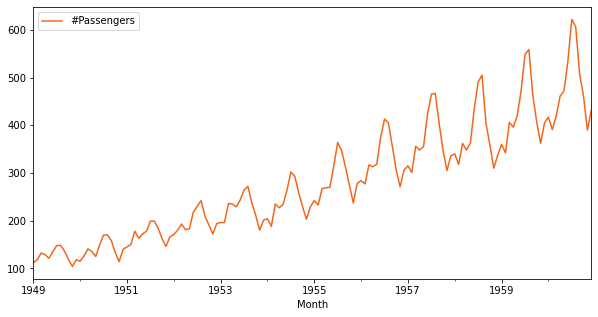
\includegraphics[width=0.6\textwidth]{airpassengers.png}
\caption{Air Passengers.}
\label{figure:air_passengers}
\end{figure}

\begin{sourcecode}
{\scriptsize \begin{verbatim}
from nescience.timeseries import TimeSeries

data = pd.read_csv("data/AirPassengers.csv", index_col=["Month"], parse_dates=True)
X = np.array(data["#Passengers"]).reshape(-1, 1)

ts = TimeSeries(auto=False)
ts.fit(data)
mscd = ts.auto_miscoding(max_lag=36)
\end{verbatim}}
\end{sourcecode}

As we can see in Figure \ref{figure:auto-miscoding} there is a peak on the value of adjusted automiscoding every twelve months (the distance between both time series is minimal when we the lag is a multple of a year).

\begin{figure}[h]
\centering
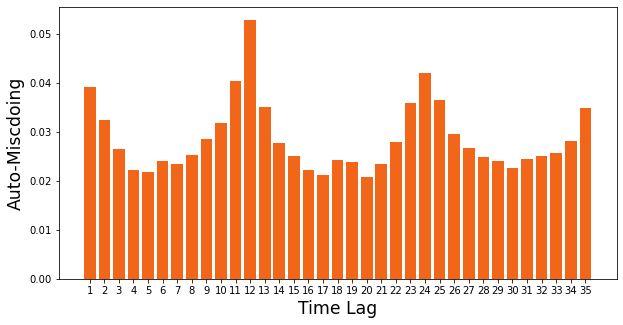
\includegraphics[width=0.6\textwidth]{auto-miscoding.png}
\caption{Auto-miscoding of Air Passengers.}
\label{figure:auto-miscoding}
\end{figure}

\end{example}

Crossmiscoding computes the inter-relation between a time series and a lagged version of a second time series. The objective is to detect if the first time series has a temporal predictive power over the second.

\begin{definition}
Let $\{\mathbf{x}_t\}$ and $\{\mathbf{y}_t\}$ be two time series composed by $n$ samples each. We define lag $k$ \emph{regular crossmiscoding} of $\{\mathbf{x}_t\}$ and $\{\mathbf{y}_t\}$ as $\hat\mu(\mathbf{x}_{x_{k+1}, x_{k+2}, \ldots, x_n}, \mathbf{y}_{x_0, x_1, \ldots, x_{(n-k)}})$. We define in the same way the concepts of \emph{adjusted crossmiscoding} and \emph{partial crossmiscoding}.
\end{definition}

\begin{example}
We are interested to determine if it possible to predict the energy consumption of the appliances of a house. The data set to study (appliances energy prediction dataset, see References below) is composed by the temperature and humidity conditions measured in the different rooms of the house every ten minutes, and the energy consumption of the appliances. The dataset also includes some information about the current weather, from a nearby weather station.

For every feature we will compute the optimal lag at which the features has the best prediction capabilities:

\begin{sourcecode}
{\scriptsize \begin{verbatim}
from fastautoml.fastautoml import Miscoding

X = pd.read_csv("../data/energydata_complete.csv", parse_dates=["date"], index_col="date")
y = X["Appliances"]
X = X.drop(["Appliances", "lights"], axis=1)

miscoding = Miscoding()
miscoding.fit(X, y)

best_lag  = list()
for i in np.arange(X.shape[1]):
    mscd = miscoding.cross_miscoding(attribute1=i, min_lag=1, max_lag=30)
    best_lag.append(np.where(mscd == np.max(mscd))[0][0] + 1)
\end{verbatim}}
\end{sourcecode}

In Figure \ref{figure:cross-miscoding} we can see a plot of the results. As we can observe, in general, for the in-house measurements we should use small lag values. However, in case of the weather conditions, bigger lags provide better results.

\begin{figure}[h]
\centering
\includegraphics[width=0.6\textwidth]{cross_miscoding_lag.png}
\caption{Cross Miscoding Lag}
\label{figure:cross-miscoding}
\end{figure}

\end{example}

\begin{remark}
The approximation to the concept of miscoding introduced in this chapter estimates the quality of individual features as predictors of a target value, and the quality of the training dataset as a whole. However, the current approximation does not take into account the existing redundancy among the features themselves. For example, it might happen that two features $\mathbf{x}_i$ and $\mathbf{x}_j$ have very low miscoding with respect to the target variable $\mathbf{y}$, but at the same time they are redundant, in the sense that they contain almost the same information. It is still an open question how to extend the concept of miscoding to take into account feature redundancy, in such a way that it is close to the theoretical definition, it can be computed efficiently, and it does not require a huge number of samples.
\end{remark}

% Auto Time Series

\subsection{Auto Time Series}

{\color{red} TODO: Introduce the auto-time series models, and clearly state what it can be expect from such models (short story: nothing)}

{\color{red} TODO: Introduce structural time series models, the state space representation, and the Kalman filter}

{\color{red} structura approach [...] different unobserved components or building blocks responsible for the dynamics of the series such as trend, seasonal, cycle, and the effects of explanatory and intervention variables are identified separately before being put together in a state space model.}

{\color{red} State space methods originated in the eld of control engineering, starting with the groundbreaking
paper of Kalman (1960). They were initially (and still are) deployed for the purpose
of accurately tracking the position and velocity of moving objects such as ships, airplanes,
missiles, and rockets [...] these ideas could well be applied to time series analysis
generally as well.}

{\color{red} In a state space
analysis the time series observations are assumed to depend linearly on a state vector that
is unobserved and is generated by a stochastically time-varying process (a dynamic system).
The observations are further assumed to be subject to measurement error that is independent
of the state vector. The state vector can be estimated or identified once a sufficient set of
observations becomes available.}

\begin{definition}
A linear Gaussian state space model for the multivariate time series $\mathbf{y} = \mathbf{y}_1, \ldots, \mathbf{y_n}$, where each observiation is a $p$ dimensional vector $\mathbf{y}_i = \{ y_{i1}, \ldots, y_{ip} \}$, is given by
\begin{equation}
\mathbf{y}_t = \mathbf{Z}_t \mathbf{\alpha}_t + \mathbf{d}_t + \mathbf{\epsilon}_t \quad \mathbf{\epsilon}_t \sim N \left( 0, \mathbf{H}_t \right)
\end{equation}
called {\color{red} space?} \emph{orbservation or measurement equation}, and
\begin{equation}
\mathbf{\alpha}_t = \mathbf{T}_t \mathbf{\alpha}_{t-1} + \mathbf{c}_t + \mathbf{R}_t \mathbf{\eta}_t \quad \mathbf{\eta}_t \sim N \left( 0, \mathbf{Q}_t \right)
\end{equation}
called \emph{state or transition equation}, where the individual summands correspond to:
\begin{align*}
 & \mathbf{y}_t \quad \text{observed or measured values,} \\
 & \mathbf{Z}_t \quad \text{design matrix,} \\
 & \mathbf{\alpha}_t \quad \text{unobserved state,} \\
 & \mathbf{d}_t \quad \text{observation intercept,} \\
 & \mathbf{\epsilon}_t \quad \text{observational disturbance,} \\
 & \mathbf{H}_t \quad \text{observational disturbance covariance matrix,} \\
 & \mathbf{T}_t \quad \text{transition matrix,} \\
 & \mathbf{c}_t \quad \text{state intercept,} \\
 & \mathbf{R}_t \quad \text{selection matrix,}  \\
 & \mathbf{\eta}_t \quad \text{state disturbance, and} \\
 & \mathbf{Q}_t \quad \text{state disturbance covariance matrix}
\end{align*}
\end{definition}

{\color{red} The $p \times m$ matrix $Z_t$ links the observation vector $y_t$ with the unobservable state vector $\alpha_t$ and may consist of regression variables.  The $m \times m$ transition matrix $T_t$ determines the dynamic evolution fo the state vector [...] the observation and state disturbances $\epsilon_t$ and $eta_t$ are assumed to be serially independent and independent of each other at all time points [...] matrix $R_t$ is an $m \times r$ selection matrix with $r < m$.}

{\color{red} The initial state vector $\alpha_1$ is assumed to be generated as $\alpha_1 \sim NID \left( a_1, P_1 \right)$, independen of the observation and estate disturbances $\epsilon_t$ and $\eta_t$. Mean $a_1$ and variance $P_1$ can be treated as given konw.}

{\color{red} Talk about initialization?}

For example, if the time series $\mathbf{y}$ is unidimensional and the state space model is time invariant (only $\mathbf{y}_t$ and $\mathbf{\alpha}_t$ depends on $t$, being the rest of the summands constant), a model with $m$ unobserved stares will be given by
\[
y_t = [ z_1 \ldots z_m ]
\begin{bmatrix}
  z_{1} \\
  \vdots \\
  z_{n}
\end{bmatrix}
+ d_{t} + \epsilon_{t}
\]

Some of the most common time series models are particular cases of the state-space model (see Example XX).

\begin{example}
\end{example}

{\color{red} TODO: Explain the Kalman filter}

The \emph{Kalman filter} is a recursive formula that provides an optimal estimate for the unknown state in a state space model. At each time step $t$, the Kalman filter computes the predicted state conditional to the observations up to time $t-1$.

{\color{red} Kalman filter can be use for filtering, prediction and smoothing. Here we are only interested in prediction [...] forward pass [...] recursive formulas}

\begin{definition}
\begin{equation}
\begin{split}
  & \mathbf{a}_{t+1} = \mathbf{T}_t \mathbf{a}_t + \mathbf{K}_t \mathbf{v}_t  \\
  & \mathbf{K}_t = \mathbf{T}_t \mathbf{P}_t \mathbf{Z}_t^T \mathbf{F}_t^{1} \\
  & \mathbf{v}_t = \mathbf{y}_t  - \mathbf{Z}_t \mathbf{a}_t
\end{split}
\end{equation}
called \emph{prediction equations}, and
\begin{equation}
\begin{split}
  & \mathbf{F}_t = \mathbf{Z}_t \mathbf{P}_t \mathbf{Z}_t^T + \mathbf{H}_t \\
  & \mathbf{L}_t = \mathbf{T}_t - \mathbf{K}_t \mathbf{Z}_t \\
  & \mathbf{P}_{t+1} = \mathbf{T}_t \mathbf{P}_t \mathbf{L}_t^T + \mathbf{R}_t \mathbf{Q}_t \mathbf{R}_t^T
\end{split}
\end{equation}
called \emph{updating equations}.
\end{definition}

\begin{example}
{\color{red} TODO: Provide an example where we can see how the Kalman filter integrates the predicted probability distribution and observed probability distribution to make a prediction}
\end{example}

{\color{red} TODO: Examplain the space search algorithm}

\begin{example}
{\color{red} TODO: Provide an example of auto-time series}
\end{example}

%
% Section: Anomaly Detection
%

\section{Anomaly Detection}

As we have seen in Section XXX, the main problem in the area of anomalies detection is that we do not have a precise mathematical definiton of what an anomaly is. Given a dataset, in this book we propose to equate the concept of abnormal samples with that of incompressible samples, and study its consequences. The essence of this chapter is that learning is about finding regularities in a dataset, and finding regularities is what data compression is about. We have also seen that the best model is the one that minimizes the sum of the length of the model plus the length of the data given the model. This optimal model divides our dataset into two disjoint subsets, the compressible part, and the incompressible part. It is the former in which we are interested in this section, since being incompressible means that they cannot be explained by the model, that is, they are model-based anomalies given the best possible model.

{\color{red} Fix the following definition.}

\begin{definition}
Let $\emph{X}$ be a dataset composed by $p$ features and $n$ samples, $\mathbf{y}$ the target variable, and $\mathit{M}$ a model such that the nescience $N \left( \mathbf{X}, \mathit{M} \right)$ is minimal. Let $\hat{y} = \mathit{M} \left( \mathbf{X} \right)$ be the predicitons made by the model $\mathit{M}$ over the vectors of $\mathbf{X}$. We define the \emph{anomaly subset} of $\mathbf{X}$, denoted by $\mathcal{A}_\mathit{M}^\mathbf{X}$, to the set of $X$ such that $y \neq \hat{y}$.
\end{definition}

The \texttt{nescience.anomalies} class allow us to identify the anomaly subset, that is, the collection of samples that do not match the regularity patterns found in the rest of the dataset. In Example \ref{ex-abnormal_boston_houses} we will see how to apply this class to indentify houses with abnormal low prices, and to explain why they are cheaper.

\begin{example}
\label{ex-abnormal_boston_houses}
In this example we will use the Boston House Price dataset provided by the \texttt{scikit-learn} toolkit. The dataset contains 13 predictive features (both, numeric and categorical) measuring different characteristics of the houses, such as number of rooms, age, etc., and the target is the median value of owner-occupied homes. The dataset is composed by five hundred samples. We are interested in to identify those house that have an abnormally low price, that is, houses that given their characteristics (number of rooms, size, etc) should have a higher price.

\begin{sourcecode}
{\scriptsize \begin{verbatim}
from sklearn.datasets import load_boston

data = load_boston()
X    = data.data
y    = data.target
\end{verbatim}}
\end{sourcecode}

We have to train a "knowledge model", that is, find the best model that explains the target variable given the predictors, without overfitting. By default, the \texttt{anomalies} class uses the AutoML capabilities provided by the \texttt{nescience} library.

\begin{sourcecode}
{\scriptsize \begin{verbatim}
from nescience.anomalies import Anomalies

model = Anomalies(X_type="mixed", y_type="numeric")
model.fit(X, y)
\end{verbatim}}
\end{sourcecode}

Finally, we have to select those samples for which the actual price is smaller than the one predicted by the model.

\begin{sourcecode}
{\scriptsize \begin{verbatim}
anomalies = model.get_anomalies("smaller")
X.shape, anomalies.shape
((506, 13), (25,))
\end{verbatim}}
\end{sourcecode}

As we can see, there are 25 houses with abnormally low price.
\end{example}

The \texttt{anomalies} class also allow us to classify the identified anomalies according to the characteristics they share.


Let's see which are the best attributes that describe those abnormal houses.

\begin{sourcecode}
{\scriptsize \begin{verbatim}
model.get_classes(n_dims=1, an_type="smaller", filter_balancedness=True,
                  filter_redundancy=False, filter_repeated_attrs=False)

Attribute1	Attribute2	Inertia	        N Class 0	N Class 1	Ratio
2	        None	        154.953975	9	        16	        0.36
4	        None   	        0.090593	6	        19	        0.24
5	        None	        5.002437	17	        8	        0.68
7	        None	        20.352117	6	        19	        0.24
8	        None	        77.611111	18	        7	        0.72
9	        None	        41737.11111	7	        18	        0.28
10	        None	        26.577436	13	        12	        0.52
12	        None	        430.294828	18	        7	        0.72
\end{verbatim}}
\end{sourcecode}

According to the inertia, the best attribute that allow us to classify the anomalies is the number 4 (nitric oxides concentration). This attribute divides the abnormal houses into two clusters of size 6 and 19. Let's see how the house's price is affected by this dimension.

\begin{sourcecode}
{\scriptsize \begin{verbatim}
from sklearn.linear_model import LinearRegression
import matplotlib.pyplot as plt
        
lr = LinearRegression()
lr.fit(X[:,4].reshape(-1, 1), y)
        
plt.scatter(X[:,4].reshape(-1, 1), y)
plt.plot(X[:,4], lr.intercept_ + lr.coef_ * X[:,4], color="red")
plt.xlabel(data.feature_names[4])
plt.ylabel("Price")
\end{verbatim}}
\end{sourcecode}

\begin{figure}[h]
\centering
\includegraphics[width=0.6\textwidth]{nox_price.png}
\caption{Price as a function of NOX.}
\label{figure:nox_vs_price}
\end{figure}

The regression line suggest that the price of the houses is smaller in those areas with higher levels of nitric oxides concentration. Let's see how the anomalies are classified according to this dimension.

\begin{sourcecode}
{\scriptsize \begin{verbatim}
class0, class1 = model.get_class_points(attribute1=4, attribute2=None, an_type="smaller")

plt.hist(class0)
plt.hist(class1)
plt.ylabel("Count")
plt.xlabel(data.feature_names[4])
plt.show()
\end{verbatim}}
\end{sourcecode}

\begin{figure}[h]
\centering
\includegraphics[width=0.6\textwidth]{nox_histogram.png}
\caption{Histogram of anomalies NOX.}
\label{figure:nox_histogram}
\end{figure}

The analysis suggests that six of the houses have an abnormally low price because they are in an area with high levels of contamination. We can repeat the same analysis with the other attributes, although they have a higher inertia, so the class separation is not that evident. Please mind that there could be more than one reason why the price of a house is abnormally low. 



%
% Section: Decision Trees
%

\section{Decision Trees}
\label{sec:decision_trees}

In the last sections we have seen how to use the concepts of miscoding, inaccuracy, surfeit and nescience to evaluate the quality of datasets and models, and to automatically select a family of models and search over its hyperparameters to find the best possible description of a topic. In particular, we have studied in detail the family of binary decision trees. The procedure used in the \texttt{fastautoml} library with trees was a mix between a classical approach (a CART algorithm combined with a cost-complexity pruning), and an evaluation of candidate trees using the minimum nescience principle. In this section we are going to see a new algorithm to derive optimal trees, both for classification and regression problems, that is entirely based on the theory of nescience. The new algorithm, by design, avoids the overfitting of the training dataset without losing accuracy, it does not require the optimization of hyperparameters, thus significantly reducing the training time, and it produces much smaller and more shallow trees than traditional algorithms, facilitating the interpretability of the results.

\subsection{Algorithm Description}
\label{sub:tree_algorithm_description}

The following pseudocode shows the proposed algorithm to build a decision tree given a training dataset $(\mathbf{X}, \mathbf{y})$. The procedure is based on a breadth first traversal of trees combined with a greedy approach. It requires a function called \textsc{bestSplit()} that returns the best split of a given subset of the data into two subsets; and a second function, called \textsc{Nescience()} that provides an estimation of the nescience of the current tree. The algorithm is based on two nested loops: the external \textbf{while} loop keeps a list of the candidate nodes to grow, whereas the internal \textbf{for} loop finds the best node to grow the tree. The latter operation requires to check all possible growing options and select the one that minimizes the nescience. The exit point of the algorithm is when there are no more branches to grow. We keep track of the best nescience achieved during the building process and return the associated tree.

\begin{sourcecode}
\label{algorithm:decision_tree}
{\scriptsize \begin{verbatim}

def BUILD_TREE(data)

    nodesList <- list()
    tree <- BESTSPLIT(data)
    bestNescience <- NESCIENCE(tree)
    nodesList.append(tree)

    while not nodesList.empty()
    
        nescience <- bestNescience
        bestNode <- None
        childNode <- None
        
        for i <- 1, nodesList.length()

            node <- nodesList[i]
            
            node.child <- BESTSPLIT(node.ldata)
            tmp <- NESCIENCE(tree)
            if tmp < nescience
                nescience <- tmp
                bestNode <- i
                
            node.left <- None

        if nescience < bestNescience
            node <- nodeList[bestNode]
            bestNescience <- nescience
            nodesList.append(node.left)
                        
            if not node.left.empty() and not node.right.empty()
                nodesList.remove(bestNode)
    
    return tree
\end{verbatim}}
\end{sourcecode}

The main difference of our algorithm from other decision tree building algorithms is in the way the tree is evaluated. Instead of using only accuracy as most of the algorithms do, in addition, we take into account the complexity of the tree (surfeit) to avoid overfitting, and the quality of the subset of data used during the training process (miscoding).

\subsubsection*{Nescience}
\label{sub:tree_nescience}

The calculation of the nescience implemented in the algorithm is based on a Euclidean distance utility function (see Section \ref{sec:machine_learning_nescience}), because that one was the one that produced the best results in the tests we have performed. For the computation of miscoding and inaccuracy, we use the same techniques that the one used in the \texttt{fastautoml} library, described in Section \ref{sec:machine_learning_miscoding} and Section \ref{sec:machine_learning_inaccuracy} respectively. For the implementation of surfeit, we use the same template to describe trees that was used in the \texttt{DecisionTreeClassifier} of the \texttt{AutoClassifier} class, and that was described in Section \ref{subsec:surfeit_decision_trees}. The only difference is that we also allow equalities in the nodes (\texttt{if [attr] = [thresh]}), something not supported by the \texttt{DecisionTreeClassifier} algorithm of the \texttt{scikit-learn} library.

The generic problem of the instability of inaccuracy due to very short models, also applies to this algorithm (see Section \ref{sec:machine_learning_surfeit}), and the particular problem of the algorithms to build decision trees, in which the best local split might not be that one that minimizes the error (see Section \ref{sec:sec:machine_learning_classification}) is also relevant in this case.

The concept of nescience is used in two different ways in our algorithm. For every iteration of the \texttt{for} loop we have to decide which one of the candidate branches of the tree we should develop. Recall that the order in which we develop the branches is important, since it might happens that one branch does not get develped because that would mean increase the sufeit without a sufficiently large decrease of the inaccuracy. The second place is a the end of the \texttt{while} loop, we we keep trac of the nescience of the different building steps, to decide at the end of the algorithm with wich tree we return.

We treat regression problems as classification problems in which we discretizes the continuous target variable $\mathbf{y}$ into $n$ intervals given the number of samples, and using a uniform discretization (see Section \label{sec:codes_continuous_data}). Once the target variable has been discretized, we train a regular classification tree.

\subsubsection*{Splitting Criteria}
\label{sub:tree_splitting_criteria}

Given a subset $\mathbf{Q} \subseteq \mathbf{X}$ we have to find an split for $\mathbf{Q}$ such that the values of $\textbf{y}$ are grouped together. Recall that a split is a pair $\theta = (j,w)$, were $1 \leq j \leq p$ is a feature index and $w$ is the partition point (see Section \ref{subsec:learning_decision_trees}). A split divides the set $\mathbf{Q}$ into two disjoint subsets $\mathbf{Q}_l$ and $\mathbf{Q}_r = \mathbf{Q} \backslash \mathbf{Q}_l$. In case of a continuous variable we have that $\mathbf{Q}_l = \{\mathbf{x}_i \in \mathbf{Q} : x_{ij} \leq w\}$, and if the feature is categorical we define $\mathbf{Q}_l = \{\mathbf{x}_i \in \mathbf{Q} : x_{ij} = w\}$\footnote{Ideally, for the categorical case, instead of a single feature $w$ we should search over all the elements of the power set of the set of features $\mathcal{P} \{1, 2, \ldots, p \}$. Unfortunately, that would imply to check $2^p$ cases, something that is time-expensive from the computational point of view.}.

In Section \ref{subsec:learning_decision_trees} we saw that a common splitting criteria used in practice is to minimize the weighted entropy $\tilde{H}$ of the subsets $\mathbf{Q}_l$ and $\mathbf{Q}_r$, that is, to find an split that it is minimal $\theta^\star = \argmin_\theta \tilde{H}(\mathbf{Q},\theta)$. More explicitly, if $\mathbf{y}$ is a target vector taking values from a set of $k$ labels $\mathcal{G} = \{g_1, \ldots, g_k \}$ (either because is a categorical target or a continuous target that has been discretized into $k$ intervals), and denoting the subsets of $\mathbf{y}$ as $\mathbf{y}^l = \{y_i : \mathbf{x}_i \in \mathbf{Q}_l \}$ and $\mathbf{y}^r = \{y_i : \mathbf{x}_i \in \mathbf{Q}_r \}$, and $n_l$ and $n_r$ are the number of elements of $\mathbf{y}^l$ and $\mathbf{y}^r$ respectively, we have that
\begin{multline}
\tilde{H}(\mathbf{Q},\theta) = \frac{n_l}{n} \left( - \sum_{i=1}^k \frac{ \sum_{j=1}^{n_l} I(y^l_j = g_i)} {n_l} \log_2{ \frac{ \sum_{j=1}^{n_l} I(y^l_j = g_i)} {n_l} } \right) \\
+ \frac{n_r}{n} \left( - \sum_{i=1}^k \frac{ \sum_{j=1}^{n_r} I(y^r_j = g_i)} {n_r} \log_2{ \frac{ \sum_{j=1}^{n_r} I(y^r_j = g_i)} {n_r} } \right)
\end{multline}

In our nescience based decision tree algorithm, the splitting criteria is to minimize the total length of encoding the subsets $\mathbf{Q}_l$ and $\mathbf{Q}_r$ using optimal codes. We have to find the optimal split $ \theta^\star = \argmin_\theta \hat{K}_C(\mathbf{Q} \mid \theta) = \argmin_\theta \{ \hat{K}_{C_l}(\mathbf{Q}_l) + \hat{K}_{C_r}(\mathbf{Q}_r) \}$ where $C_l$ and $C_r$ are the optimal codes given the relative frequencies of the observed values of $\mathbf{y}^l$ and $\mathbf{y}^r$ respectively. The quantity $\hat{K}_C(\mathbf{Q} \mid \theta)$ is computed as:
\[
\hat{K}_C(\mathbf{Q} \mid \theta) = \hat{K}_{C_l}(\mathbf{Q}_l) + \hat{K}_{C_r}(\mathbf{Q}_r) = - \sum_{i=1}^k \log_2{ \frac{ \sum_{j=1}^{n_l} I(y^l_j = g_i)} {n_l} } - \sum_{i=1}^k \log_2{ \frac{ \sum_{j=1}^{n_r} I(y^r_j = g_i)} {n_r} }
\]
I this particular case (if we use as compression algorithm a code with optimal lengths, and continuous variables have been discretized) it turns out that both expressions are equivalent given the following relation:
\[
\tilde{H}(\mathbf{Q},\theta) = \frac{1}{n} \hat{K}_C(\mathbf{Q} \mid \theta)
\]
We prefer to talk of encoding length instead of weighted entropy because it has an easier interpretation in the context of the theory of nescience.

\begin{remark}
Strictly speaking, if we want to implement a decision trees search algorithm fully compliant with the minimum nescience principle, instead of using a total length encoding as splitting criteria, we should had computed the nescience at each split and select that one that makes it minimal. However, early experiments have shown that at local level it works better to group the values of $y$ than to reduce the nescience. Further research is required to confirm and explain this point.
\end{remark}

\subsubsection*{Practical Implementation}

In the web page that accompanies this book\footnote{http://www.mathematicsunknown.com} we provide an open-source implementation of our algorithm in Python. Our software can be used together with other machine learning tools from the \texttt{scikit-learn} library, since we adhere to the their API guidelines. For example, our algorithm can be used as part of an ensemble of classifiers, like the \texttt{BaggingClassifier} meta-estimator, or the results of the classification could be cross-validated with tools like \texttt{cross\_val\_score}. As an example, to provide a model for the breast cancer dataset, we could do something like the following:

\begin{sourcecode}
{\scriptsize \begin{verbatim}
from NescienceDecisionTree import NescienceDecisionTreeClassifier
from sklearn.datasets import load_breast_cancer

data = load_breast_cancer()

model = NescienceDecisionTreeClassifier()
model.fit(data.data, data.target)
print("Score: ", model.score(data.data, data.target))
\end{verbatim}}
\end{sourcecode}

\subsection{Algorithm Evaluation}
\label{sub:algorithm_evaluation}

In this section we are going to evaluate our new algorithm, and compare its performance against the well-known algorithm CART. CART, \emph{Classification and Regression Trees}, is the de-facto standard algorithm used in the machine learning industry for the derivation of decision trees. For this particular experiment we have used the CART implementation provided by \texttt{scikit-learn}.

Figure \ref{figure:data_error_cart} shows a synthetic dataset consisting of $1000$ random points lying on a two dimensional plane, where all the points with an $X1$ attribute less than $50$ are colored blue, and the rest as red. We have artificially introduced a red point, simulating a measurement error, in the blue area. The black lines correspond to the decisions performed by CART. Since the CART algorithm will not stop until all the points have been properly classified, we have to specify an expected count condition to limit the number of splits. The figure correspond to the tree generated by CART setting the \texttt{min\_samples\_leaf} hyperparameter to $5$.

\begin{figure}[h]
\centering
\includegraphics[width=0.6\textwidth]{data_error_cart.jpg}
\caption{Synthetic dataset with CART algorithm splits.}
\label{figure:data_error_cart}
\end{figure}

The tree obtained by applying our algorithm to the dataset of Figigure \ref{figure:data_error_cart} can be seen in Figure \ref{figure:data_error_nes}. The nescience based algorithm does not try to model the error point, since the gain due to an increment in the accuracy does not compensate the surfeit introduced in the model. Recall that the algorithm stops when the total nescience of the tree, based on the measures of miscoding, inaccuracy and surfeit, does not decrease when adding new nodes to the tree. Our algorithm presents a lower sensitivity to the errors found in datasets, at least if the number of errors is small compared with the number of valid points.

\begin{figure}[h]
\centering
\includegraphics[width=0.4\textwidth]{small_error.jpg}
\caption{Decision tree obtained by the nescience algorithm.}
\label{figure:data_error_nes}
\end{figure}

Our second experiment, again with synthetic dataset, is depicted in Figure \ref{figure:blobs}. There, we create two isotropic Gaussian blobs that partially overlap. We start with a standard deviation of $2.5$ for each cluster, so they are easy to separate, and we increase the standard deviation in increments of $0.01$, until we reach $4.5$, which causes significant overlaps. For each value of the standard deviation, we run the experiment $100$ times and we compute the average accuracy for the two algorithms using different datasets for training (70\% of the data) and testing (30\% of the data). The results of this experiment are shown in Figure \ref{figure:accuracy_blobs}.

\begin{figure}[h]
\centering
\includegraphics[width=0.6\textwidth]{blobs.png}
\caption{Isotropic Gaussian Blobs.}
\label{figure:blobs}
\end{figure}

As we can see, the performance of both algorithms, in terms of accuracy, is similar. However we should note that the hyperparameter \texttt{minimum\_leaf\_size} of the CART algorithm has been optimized to achieve the best accuracy. For this particular experiment, the best value was achieved with a minimum leaf size of 26 points. By definition, given the fact that CART has one degree of freedom more than the nescicence algorithm, it should produce better accuracy; something that it is not observed (both algorithms have a mean accuracy of $0.87$.

\begin{figure}[h]
\centering
\includegraphics[width=0.6\textwidth]{accuracy_blobs.png}
\caption{Accuracy of Isotropic Gaussian Blobs.}
\label{figure:accuracy_blobs}
\end{figure}

For each iteration of the experiment, we have also computed the average number of nodes, including internal and leaf nodes, required by the models to properly classify the clouds in the dataset. The results of this measurement are show in Figure \ref{figure:length_nodes}. Our algorithm requires an average of $4$ nodes compared to $23$ nodes for the CART algorithm. Moreover, our algorithm is more stable than CART, in the sense that it produces models of similar complexity when it gets similar input datasets (a standard deviation of $0.31$ compared to $3.77$ for CART).

\begin{figure}[h]
\centering
\includegraphics[width=0.6\textwidth]{nodes_blobs.png}
\caption{Number of Nodes.}
\label{figure:length_nodes}
\end{figure}

In Figure \ref{figure:blob_max_depth} we show the maximum depth of the tree, defined as the longest path from the root of the tree to any of its leaves. The maximum depth of the tree is a good measure of the average time it will require for the model to provide a classification. The nescience algorithm has an average depth of $1.6$ nodes, whereas the average depth yielded by the CART algorithm is $4.8$ nodes.

\begin{figure}[h]
\centering
\includegraphics[width=0.6\textwidth]{max_depth.png}
\caption{Maximum depth of the model.}
\label{figure:blob_max_depth}
\end{figure}

The last part of the evaluation consists in comparing the performance of our algorithm and CART with a collection real datasets. More specifically, we have selected $12$ well known datasets from the UCI Machine Learning Repository. The selected datasets are: diagnosis of breast cancer (\texttt{cancer}), optical recognition of handwritten digits (\texttt{digits}), predicting protein localization sites in gram-negative bacteria (\texttt{yeast}), classification of NASA space shuttle data (\texttt{shuttle}), classification of blocks in web pages (\texttt{page}), segmentation of outdoor images (\texttt{image}), predicting the age of abalones from physical measurements (\texttt{abalone}), predicting the quality of red and white variants of Portuguese wine (\texttt{wine}), filter spam emails (\texttt{spam}), wall-following robot navigation (\texttt{wall}), classification of land use based on Landsat satellite images (\texttt{landsat}), and distinguishing signals from background noise in the MAGIC gamma telescope images (\texttt{magic}). For each dataset, we have repeated the experiment 100 times, by randomly selecting the training (70\%) and testing (30\%) subsets at each iteration.

\begin{figure}[h]
\centering
\includegraphics[width=0.6\textwidth]{cart_nescience_accuracy.png}
\caption{Maximum depth of the model.}
\label{figure:cart_nescience_accuracy}
\end{figure}

In Figure \ref{figure:cart_nescience_accuracy} we compare the accuracy of the resulting models obtained by applying the CART algorithm and the nescience algorithm to the above datasets. In $4$ of the $12$ datasets, our algorithm provides better accuracy than CART. In the remaining $8$ cases, the accuracy is, on average, less than $1\%$ smaller.

\begin{figure}[h]
\centering
\includegraphics[width=0.6\textwidth]{cart_nescience_nodes.png}
\caption{Maximum depth of the model.}
\label{figure:cart_nescience_nodes}
\end{figure}

In Figure \ref{figure:cart_nescience_nodes} it is shown a comparison of the total number nodes (internal nodes plus leaf nodes) of the resulting models. Only for one of the datasets (\texttt{digits}), our model produces a slightly more complex tree that those generated by CART. In the rest of the cases, the number of nodes in the trees generated by the nescience algorithm have between two and three orders of magnitude fewer nodes (in this figure the $y$ axis is in logarithmic scale).

\begin{figure}[h]
\centering
\includegraphics[width=0.6\textwidth]{cart_nescience_depth.png}
\caption{Maximum depth of the model.}
\label{figure:cart_nescience_depth}
\end{figure}

Finally, in Figure \ref{figure:cart_nescience_depth} we provide a comparison of the depth of the tree of the resulting models. Our algorithm always yields a shallower tree than the CART algorithm.

We would like to mention that the nescience algorithm is hihgly robust with respect to the compressor selected or the nescience function implemented. In Table \ref{table:nescience_functions}, we have apply the nescience algorithm to the datasets described above, and evaluate different alternatives for the definition of the nescience function $N (X , M )$: arithmetic mean $(\mu(M , D) + \iota(X , M ) + \sigma(M, D))/3$, geometric mean $(\mu(M , D) + \iota(X , M ) + \sigma(M, D)) 1/3$ , harmonic mean $3 / (\mu(M , D) + \iota(X , M ) + \sigma(M, D)) -1 )$, Euclidean distance $(\mu(M , D) + \iota(X , M ) + \sigma(M, D)) 1/3$, sum $\mu(M , D) + \iota(X , M ) + \sigma(M, D)$, and product $\mu(M , D) + \iota(X , M ) + \sigma(M, D)$. The table shows limited difference between the different functions. 

\begin{table}[h]
\label{table:nescience_functions}
\centering
\begin{tabular}{l l l l l l l l}
\toprule
 & \textbf{Euclid} & \textbf{Arithmetic} & \textbf{Geometric} & \textbf{Product} & \textbf{Addition} & \textbf{Harmonic} \\
\midrule
Accuracy & 0.758 & 0.784 & 0.803 & 0.803 & 0.784 & 0.81 \\
Stdev & 0.051 & 0.041 & 0.033 & 0.033 & 0.041 & 0.038 \\
\bottomrule
\end{tabular}
\caption{Comparison of nescience functions}
\end{table}

Similarly, Table \ref{table:compressor} shows the performance of our algorithm when using the LZMA, zlib, and bz2 compressors. We observe that all of them yield similar performance. The above results suggest that the performance our algorithm is independent of the specific choice made for either implementation aspect.

\begin{table}[h]
\label{table:compressor}
\centering
\begin{tabular}{l l l l}
\toprule
 & \textbf{bz2} & \textbf{lzma} & \textbf{zlib} \\
\midrule
Accuracy & 0.813 & 0.804 & 0.81 \\
Stdev & 0.03 & 0.045 & 0.038 \\
\bottomrule
\end{tabular}
\caption{Comparison of compressors}
\end{table}

We emphasize that the CART algorithm requires to optimize a configuration hyperparameter in order to obtain good results, whereas the algorithm proposed in this book does not require from this optimization.

Shallower trees means faster forecasting times when the models used in production, since the number of \texttt{if-else} conditions to be evaluated is smaller. Moreover, smaller trees makes easier to interpret the results by human analysts. and much shorter training times, something very relevant in case of training ensembles of trees, like random forest or boosted trees (although the use of ensembles of models is highly discouraged by the theory of nescience, given their high surfeit).

%
% Section: Algebraic Model Selection
%

\section{Algebraic Model Selection}

As it was the case for the definition of nescience based on the encyclopedic description of research topics, the nescience of structured datasets can be used to evaluate alternative descriptions of research topics (mathematical models), and to identify how far these descriptions are from an ideal perfect knowledge. This evaluation could be used to identify those topics which require further research. Moreover, the same methodology could be applied to collections of datasets to identify our current knowledge of research areas (collections of topics).

If we combine the concept of nescience of a model, with our concepts of relevance and applicability of research topics, we could apply our methodology for the assisted discovery of interesting questions to collections of datasets; a very useful methodology now that big datasets are becoming widely available.

In order to evaluate the methodology developed, we are going to apply it to a particular research topic: \emph{Multipath Wave Propagation and Fading}. The problem at hand is to understand the effect of a propagation environment on a radio signal, such as the one used by wireless devices. The signals reaching the receiving antenna could follow multiple paths, due to atmospheric reflection and refraction, and reflection from water and objects such as buildings. The effects of these multiple wave paths include constructive and destructive interference (fading), and phase shifting of the original signal, resulting a highly complex received signal (see Figure \ref{fig:Multipath-Signal-Propagation}).

\begin{figure}[h]
\centering\includegraphics[scale=0.5]{fading}
\caption{\label{fig:Multipath-Signal-Propagation}Multipath Signal Propagation}
\end{figure}

In many circumstances, it is too complicated to describe all reflection, diffraction and scattering processes that determine the different paths the signal will follow. Rather, it is preferable to describe the probability (stochastic model) that the received signal attains a certain value. We are interested in to analyze how well these stochastic models (our current knowledge) are able to describe what happen in reality.

The \emph{Rayleigh fading model} assumes that the magnitude of a signal will vary randomly, or fade, according to a Rayleigh distribution (the radial component of the sum of two uncorrelated Gaussian random variables). The Rayleigh probability density function of the power signal is given by:

\[
P_{\sigma}\left(x\right)=\frac{1}{\sigma}\exp\left[-\frac{x}{\sigma}\right]
\]

where $\sigma$ is the mean of the received signals. Rayleigh fading is viewed as a reasonable model for the effect of heavily built-up urban environments, when there is no dominant propagation along a line of sight between the transmitter and receiver.

The Rice or \emph{Rician distribution} describes the power of the received signal when the target consists in many small scatterers of approximately equal strength, plus one dominant scatterer whose individual received signal equals all that of all the small scatterers combined (there is a dominant line of sight). The probability density function of the power of the received signal is given by:

\[
P(x)=\frac{1}{\bar{\sigma}}\left(1+a^{2}\right)\exp\left[-a^{2}-\frac{x}{\bar{\sigma}}\left(1+a^{2}\right)\right]I_{0}\left[2a\sqrt{\left(1+a^{2}\right)\frac{x}{\bar{\sigma}}}\right]
\]


where $\bar{\sigma}$ is the mean of the received signals, and it is equal to $\bar{\sigma}=\left(1+a^{2}\right)\bar{\sigma}_{R}$, being $a^{2}\bar{\sigma}_{R}$ the power of the dominant scatterer, and $I_{0}$ is the modified zeroth order Bessel function of the first kind.

An experiment (see Figure \ref{fig:Experimental-Set-Up}) was set up to collect a real dataset to analyze. The experiment was run on a $135 m^2$ office full of obstacles (interacting objects). The transmitter was an Odroid C1 Linux computer with a Ralink RT5370 USB Wifi adapter. The receiver was a (fixed in space) Motorla Moto G mobile phone. Data was collected using the Kismet \footnote{https://www.kismetwireless.net/index.shtml} platform (an 802.11 layer2 wireless network detector, sniffer, and intrusion detection system), with some ad hoc, home made, software extensions, mostly for data aggregation. A total of 3,177 samples (power level measured in dBm) were collected during one hour experiment.

\begin{figure}[h]
\centering\includegraphics[scale=0.2]{experiment}
\caption{\label{fig:Experimental-Set-Up}Experimental Set Up}
\end{figure}

Next table summarizes the results of applying the three considered models (uniform, Raylegh and Rice) and the optimal encoding using a Huffman code:

\begin{table}[h]
\centering
\begin{tabular}{l l l}
\toprule
\textbf{Model} & \textbf{LDM} & \textbf{Nescience} \\
\midrule
Uniform & 17,351 & 1.30 \\
Rayleigh & 13,229 & 0.75 \\
Rice & 11,118 & 0.47 \\
Huffman & 7,541 & - \\
\bottomrule
\end{tabular}
\caption{Nescience of Models}
\end{table}

The uniform model, that is, assuming zero knowledge about the topic covered by the dataset, has a nescience of 1.30. This value is a kind of upper level for the nescience associated with that particular topic and dataset; any model with a higher nescience should be classified as zero knowledge model. If we introduce the knowledge that in a environment with multiple obstacles the signal propagation can be described as a Gaussian process (Rayleigh distribution), we are able to decrease our nescience to 0.75, that is, there were a 43\% improvement in our understanding of the topic. If we add the knowledge that there is usually a strongly dominant signal seen at the receiver caused by a line of sight between the antenna and the mobile phone (Rician distribution), the nescience decreases to 0.47, and so, we have achieved an additional 23\% gain in our understanding. Given that numbers we can conclude that the Rayleigh model increases our knowledge with respect to the uniform model, and that the Rice model does so with respect to Rayleigh. However, the nescience of this last model is 0.47. That means that there still patterns in the dataset that are not explained by the Rice model, or what it is equivalent according to our methodology, there is still some knowledge to discover and learn.

The methodology has been applied to a dataset gathered in a single experiment under a controlled environment, since the goal of this Chapter was to provide a methodology to quantify the nescience of structured datasets, not to evaluate models for signal propagation and fading. In order to to conclude that, in general, the Rice model is an improvement over Rayleigh, a more realistic experiment is required, with multiple datasets gathered in real environments.

%
% Section: The Analysis of the Incompressible
%

\section{The Analysis of the Incompressible}

As we have said in Chapter {chap:Introduction}, one of the reasons to understand how things work is to understand the cause-effect relation in systems. We are interested in this cause/effect relation in two ways. That is, if we want to see an effect in a system, we want to understand wich causes trigger that effect. Also, and perhaps more interesting, if we have observed an (probably undesired effect) in a system we would like to discover what has caused that effect, so we can fix it, and revert the normal situation.

We could use the theory of nescience to model, and modify, those uncommon effect, by means of training a model and looking at the incompressible part of the data.


A model $\mathcal{M}$ for a dataset $\mathcal{D} = (X, y)$ is a compressed version of that dataset, since the length of the dataset given the model $l(\mathcal{D} \mid \mathcal{M})$ is smaller that then length of the original dataset $l(\mathcal{D})$. The model $\mathcal{M}$ is composed by the regularities found in the dataset (subject to the algorithm used and the families of models considered). What it is left, $\mathcal{D} \mid \mathcal{M}$ is the incompressible part of the dataset, that is, those samples that have no regularity at all, or present a regularity that requires a description longer than the length of the raw data.

In this section we are going to show the practical applications of analyzing what it is left, that is, the incrompressible samples of a dataset. An element that is incompressible represents a very unlikely, or uncommon, situation of the entity being studied. A incompressible element does not necessarily means a problem, since if a problem is sufficiently common, it can be compressed. An incompressible element is something than cannot be explained given the normal behaviour of the system. Of course, all of this is assuming that our dataset has no errors.

Once we have found a model that has the lowest possible nescience for a dataset, we could separate those elements that have not been compresed, denoted by XX, and fit a second model. We could argue that it does not make any sense to model the incompressible part, since, it is incompressible. However, the incompressible part is incompressible with respect to the original entity under study, that is, the global systen. And in this new case, we are studying a different entity, namely, the uncommon parts of an entity. It might happen that we can find regularities in this new entity.



%
% Section: References
%

\section*{References}
\label{sec:ML_references}

A insightful description of the differences between explanation models and predictive models, how these models are used in different scientific disciplines, and what are the implications for the process of statistical modeling can be found in \cite{shmueli2010explain}.

The application of the minimum description length principle to the identification of optimal decision trees have been proposed in \cite{quinlan1989inferring}, further refined and clarified in \cite{wallace1993coding}; however the coding method proposed by those authors is different from the one used in this book.

In our web page can be found an implementation of the decision tree following the guidelines defined in []. 


The Minimum Description Length \cite{grunwald2007minimum} and the Minimum Message Length \cite{wallace2005statistical} techniques have been applied to the problem of inferring decision trees in \cite{quinlan1989inferring}, later on clarified and extended in~\cite{wallace1993coding}, in \cite{mehta1995mdl} as a technique for pruning, and in \cite{rastogi1998public}, among others. Although the underlining concepts behind the cost function proposed in this chapter are the same (namely, that learning is equivalent to the capability to compress), our approach is very different from the ones described in these works.

An excellent survey of the available discretization methods can be found in~\cite{garcia2013survey}; in the paper the authors also propose a taxonomy to classify existing methods based in their properties and they conduct an extensive comparative experimental study. The proportional discretization method used to compute miscoding is introduced in~\cite{yang2009discretization}, where there is also a theoretical justification of why this method reduces the bias and the variance of the discretized variable.

{\color{red} TODO: Find the original reference of the AirPassengers dataset.}

{\color{red} TODO: Find the original reference of the Appliance energy consumption dataset. https://archive.ics.uci.edu/ml/datasets/Appliances+energy+prediction}





%
% CHAPTER: Software Engineering
%

%
% CHAPTER 9.- Software Engineering
%

\chapterimage{AnalyticalEngine.pdf}

\chapter{Software Engineering}
\label{chap:Software-Engineering}

{\color{red} TODO: Change chapter image}

{\color{red} TODO: Rewrite this introduction}

Our final example of how to apply the theory of nescience in practice comes from the area of software engineering. The goal of this example is to show how we can apply the concept of nescience to a problem where there are no descriptions. As I have said, what it is a description depends on the particular application at hand.

In the particular case of software engineering we want to solve two related problems. The fist one is to quantitatively measure how mature is a particular software platform. The second one is how to discover new software tests, that have not been considered by the programmers, in that way we could increase the quality of the software.

The relevance will be based on software modules and data flow, and the nescience will be based on the number of lines of code for these modules. The rationale is that very well understood task are usually coded in libraries, meanwhile not very well understood problems are usually resolved ad-hoc.

Of course, the above statement is just conjectures that need more research to be confirmed, perhaps analyzind hunderd of software project, and perhaps, performing some experiments. The goal of this chapter is to show how the theory of nescience can be applied to other areas than scientific research, not to provide a quantitative measure of software quality.

\section{Redundancy of Software}

The concept of nescience applied to software engineering allow us to measure how immature is a particular software application or platform. As it was the case for scientific research topics, if we can compress a source code, probably we do not fully understand how to solve the problem at hand. The rationale is that immature software usually contains a lot of duplicated, redundant, code; meanwhile mature software it is usually composed of generic functions and libraries that provide near optimal solutions to common problems. As a consequence, if a code contains redundant elements there must exists a better way to solve the problem.

In this section we are going to study and compare the nescience of three software platforms in the area of database management systems: SQLite, PostgreSQL and Cassandra. The first two, SQLite and PostgreSQL, are relational database management systems based on SQL, and the third one, Cassandra, is a noSQL database (knowledge of relational databases or SQL is not required to understand this chapter). SQLite and PostgreSQL platforms are based on the C programming language, meanwhile Cassandra is written in Java. The three platforms are publicly available open source software, so the reader can repeat the experiments himself.

\subsubsection*{SQLite}

SQLite\footnote{http://www.sqlite.org}, according to the description from its web home page, \emph{is an in-process library that implements a self-contained, serverless, zero-configuration, transactional SQL database engine}. Unlike other relational databases, SQLite is not based on a client-server model, instead it is composed by a highly compact library (usually less than 500 KiB) that reads and writes directly to ordinary disk files. In fact, in SQLite a complete database with its multiple tables, indices, triggers, and views, is contained in a single disk file.

Table \ref{tab:Nescience-SQLite} provides a compilation of the results of the analysis of a selection of versions of SQLite along 15 years of continuous development (first release was published in August 2000). The columns of the table represent: the version number, the number of source code lines, the size (number of bytes) of the source code, and the size (number of bytes) of the compressed version of the source code (using the Linux tool {\tt gzip}). The final column contains the nescience associated to each version.

The analysis was performed in a Linux-based machine. The command issued to compute the number of source lines of each version was:

\begin{verbatim}
# find SQLite-1_0/src -name '*.[chyl]' -exec cat {} \; > total-1.0
\end{verbatim}

\begin{table}
\begin{centering}
\begin{tabular}{|c|c|c|c|c|}
\hline 
Version & Lines & Size & Compressed & Nescience\tabularnewline
\hline
\hline
1.0 & 11,668 & 363,025 & 84,317 & 3.31 \tabularnewline
\hline
2.0 & 20,629 & 623,058 & 151,382 & 3.12 \tabularnewline
\hline
2.1 & 22,389 & 681,026 & 165,631 & 3.11 \tabularnewline
\hline
2.2 & 22,829 & 695,475 & 169,191 & 3.11 \tabularnewline
\hline
2.3 & 24,246 & 745,092 & 181,251 & 3.11 \tabularnewline
\hline
2.4 & 26,574 & 822,638 & 201,335 & 3.09 \tabularnewline
\hline
2.5 & 30,110 & 943,328 & 231,555 & 3.07 \tabularnewline
\hline
2.6 & 31,154 & 977,407 & 238,490 & 3.10 \tabularnewline
\hline
2.7 & 31,667 & 995,136 & 243,210 & 3.09 \tabularnewline
\hline
2.8 & 35,357 & 1,117,115 & 274,299 & 3.07 \tabularnewline
\hline
3.0 & 49,197 & 1,547,363 & 390,292 & 2.96 \tabularnewline
\hline
3.1 & 54,646 & 1,722,646 & 437,335 & 2.94 \tabularnewline
\hline
3.2 & 55,940 & 1,763,913 & 449,046 & 2.93 \tabularnewline
\hline
3.3 & 65,498 & 2,070,135 & 529,485 & 2.91 \tabularnewline
\hline
3.4 & 82,288 & 2,606,260 & 666,321 & 2.91 \tabularnewline
\hline
3.5 & 86,369 & 2,737,174 & 700,228 & 2.91 \tabularnewline
\hline
3.6 & 97,864 & 3,093,778 & 790,732 & 2.91 \tabularnewline
\hline
3.7 & 126,341 & 4,158,239 & 1,080,647 & 2.85 \tabularnewline
\hline
3.8 & 148,506 & 4,923,732 & 1,274,720 & 2.86 \tabularnewline
\hline
3.9 & 166,744 & 5,583,265 & 1,446,884 & 2.86 \tabularnewline
\hline
3.10 & 168,451 & 5,636,155 & 1,458,698 & 2.86 \tabularnewline
\hline
\end{tabular}
\par\end{centering}
\caption{Nescience of SQLite}
\label{tab:Nescience-SQLite}
\end{table}

Figure \ref{fig:Nescience-of-SQLite} depicts the evolution of the nescience of the SQLite platform along the different versions analyzed. As it can be observed, in general, the nescience decrease for each new release: from a nescience of 3.23 for the first, initial release, to a nescience of 2.86 in the latest published version. This behavior of nescience in SQLite is the expected behavior of a software platform that has been designed with a highly targeted goal in mind. Each new release of SQLite is focused in doing better what the software already does, instead of adding a lot of new functionality. Given the evolution of the nescience, we could say that SQLite is a software where for every new release we know better how it manage small restational databases.

\begin{figure}[h]
\centering\includegraphics[scale=0.5]{SQLite_nescience}
\caption{\label{fig:Nescience-of-SQLite}Nescience of SQLite}
\end{figure}

\subsubsection*{PostgeSQL}

PostgreSQL\footnote{http://www.postgresql.org} is a full-featured open source object-relational database system, with a strong emphasis in reliability, data integrity, and correctness. PostgreSQL provides advanced database management capabilities, like tablespaces, data replication, fault tolerance, hot backups, and many others. PostgreSQL evolved from another database, the Ingres project, at the University of California, Berkeley. The team released version 1 of the new database to a small number of users in 1989, version 2 with a re-written rules system in 1990, and version 3 in 1991. After releasing version 4.2 in 1994 the project ended. All those initial releases of PostgreSQL were not included in the analysis because they are not open source. In 1996, the project was renamed to its current name PostgreSQL to reflect its support for the language SQL, and moved to an open source MIT-style license, which enabled other developers to modify and extend the source code. The first open source PostgreSQL release was version 6.0 from 1997. Currently, PostgreSQL is developed and maintained by the \emph{PostgreSQL Global Development Group}, that comprises companies and individual contributors.

Table \ref{tab:Nescience-PostgreSQL} provides a compilation of the results of the analysis of a selection of versions of PostgreSQL along 25 years of development. The columns in table have the same meaning than in Table \ref{tab:Nescience-SQLite}. The command issued to compute the number of source lines was:

\begin{verbatim}
# find postgresql-1_0/src -name '*.[chyl]' -exec cat {} \; > total-1.0
\end{verbatim}

\begin{table}
\begin{centering}
\begin{tabular}{|c|c|c|c|c|}
\hline 
Version & Lines & Size & Compressed & Nescience\tabularnewline
\hline
\hline
1.09 & 178,538 & 4,857,018 & 1,128,931 & 3.30 \tabularnewline
\hline
1.09 & 178,976 & 4,869,670 & 1,132,454 & 3.30 \tabularnewline
\hline
6.0 & 187,950 & 5,190,331 & 1,219,104 & 3.26 \tabularnewline
\hline
6.1 & 200,488 & 5,541,679 & 1,287,908 & 3.30 \tabularnewline
\hline
6.2 & 222,602 & 5,559,815 & 1,298,418 & 3.28 \tabularnewline
\hline
6.3.2 & 260,809 & 6,715,908 & 1,531,409 & 3.39 \tabularnewline
\hline
6.4.2 & 297,918 & 7,711,626 & 1,759,091 & 3.38 \tabularnewline
\hline
6.5 & 330,540 & 8,933,109 & 1,959,557 & 3.56 \tabularnewline
\hline
7.0 & 376,445 & 10,133,053 & 2,298,580 & 3.41 \tabularnewline
\hline
7.1 & 409,314 & 11,156,575 & 2,557,159 & 3.36 \tabularnewline
\hline
7.2 & 443,499 & 12,189,722 & 2,804,470 & 3.35 \tabularnewline
\hline
7.3 & 461,091 & 13,095,834 & 2,935,691 & 3.46 \tabularnewline
\hline
7.4 & 525,512 & 14,938,894 & 3,371,228 & 3.43 \tabularnewline
\hline
8.0 & 586,198 & 16,735,624 & 3,797,590 & 3.41 \tabularnewline
\hline
8.1 & 628,324 & 18,149,522 & 4,105,712 & 3.42 \tabularnewline
\hline
8.2 & 676,591 & 19,608,764 & 4,409,352 & 3.45 \tabularnewline
\hline
8.3 & 780,706 & 22,969,821 & 5,056,367 & 3.54 \tabularnewline
\hline
8.4 & 862,793 & 25,819,421 & 5,619,089 & 3.59 \tabularnewline
\hline
9.0 & 927,850 & 27,947,706 & 6,016,580 & 3.65 \tabularnewline
\hline
9.1 & 992,814 & 29,922,940 & 6,464,460 & 3.63 \tabularnewline
\hline
9.2 & 1,054,939 & 31,889,273 & 6,921,880 & 3.61 \tabularnewline
\hline
9.3 & 1,090,891 & 32,824,041 & 7,146,213 & 3.59 \tabularnewline
\hline
9.4 & 1,149,347 & 34,698,419 & 7,576,636 & 3.58 \tabularnewline
\hline
9.5 & 1,247,679 & 37,834,424 & 8,300,979 & 3.56 \tabularnewline
\hline
\end{tabular}
\par\end{centering}
\caption{\label{tab:Nescience-PostgreSQL}Nescience of PostgreSQL}
\end{table}

Figure \ref{fig:Nescience-of-PostgreSQL} depicts the evolution of the nescience of the PostgreSQL database engine along the different versions that have been published. As it can be observed, in general, the nescience increase for each new release: from a nescience of 3.30 for the first version analyzed to a nescience of 3.56 in the latest published version. This behavior of nescience in PostgreSQL is the expected behavior for a software platform that has the goal of provide as much new functionality as possible in every new release. Even if the developers have improved the already existing code, the immaturity of the new code produces an increment of the nescience of the platform. Given the evolution of the nescience, we could say that PostgreSQL is a software where for every new release it does more things but we know less about how it does them.

\begin{figure}[h]
\centering\includegraphics[scale=0.5]{PostgreSQL_nescience}
\caption{\label{fig:Nescience-of-PostgreSQL}Nescience of PostgreSQL}
\end{figure}

\subsubsection*{Cassandra}

Apache Cassandra\footnote{http://cassandra.apache.org} is an open source distributed database management system focused in scalability and high availability of data. Cassandra can provide near linear data scalability and fault-tolerance on commodity hardware. Cassandra data model is based on column indexes instead of the normalized tables of relational (SQL based) models. Cassandra was initially developed at Facebook to power their search feature, and it was released as an open source project on Google code in 2008. In 2009, it became an Apache Incubator project, and in 2010 it become a to a top-level project.

Table \ref{tab:Nescience-Cassandra} provides a compilation of the results of the analysis of a selection of version of Cassandar along 7 years of development. The columns in table have the same meaning than in Table \ref{tab:Nescience-SQLite} and Table \ref{tab:Nescience-PostgreSQL}, so the nescience of the three projects can be compared. The command issued to compute the number of source lines was:

\begin{verbatim}
# find cassandra-0.3.0/src/ -name "*.java" -exec cat {} \; > total-0.3.0
\end{verbatim}

\begin{table}
\begin{centering}
\begin{tabular}{|c|c|c|c|c|}
\hline 
Version & Lines & Size & Compressed & Nescience\tabularnewline
\hline 
\hline
0.3.0 & 50,370 & 1,747,132 & 296,565 & 4.89 \tabularnewline
\hline
0.4.2 & 35,386 & 1,217,575 & 214,303 & 4.68 \tabularnewline
\hline
0.5.1 & 36,823 & 1,286,675 & 231,918 & 4.55 \tabularnewline
\hline
0.6.13 & 39,740 & 1,402,412 & 251,556 & 4.57 \tabularnewline
\hline
0.7.10 & 64,279 & 2,321,786 & 419,346 & 4.54 \tabularnewline
\hline
0.8.10 & 77,331 & 2,764,743 & 503,978 & 4.49 \tabularnewline
\hline
1.0.12 & 88,479 & 3,152,422 & 575,984 & 4.47 \tabularnewline
\hline
1.1.12 & 106,441 & 3,857,420 & 712,932 & 4.41 \tabularnewline
\hline
1.2.19 & 142,775 & 5,240,648 & 942,257 & 4.56 \tabularnewline
\hline
2.0.16 & 165,593 & 6,177,890 & 1,105,372 & 4.59 \tabularnewline
\hline
2.1.9 & 195,424 & 7,315,659 & 1,316,190 & 4.56 \tabularnewline
\hline
2.2.1 & 212,249 & 7,928,612 & 1,399,814 & 4.66 \tabularnewline
\hline
3.0.0 & 242,320 & 9,083,317 & 1,617,120 & 4.62 \tabularnewline
\hline
\end{tabular}
\par\end{centering}
\caption{\label{tab:Nescience-Cassandra}Nescience of Cassandra}
\end{table}

Figure \ref{fig:Nescience-of-Cassandra} depicts the evolution of the nescience of the Cassandra platform along the different versions that have been analyzed. As it can be observed, the nescience presents a first period in which it clearly decreased for every release, and a second period where it increases again. A possible explanation of this behavior could be that Cassandra was a highly immature project at its initial releases (a nescience of 4.89) and during these first versions the developers improved the quality of the source code, and during the second period the developers focused more in to add new functionality.

\begin{figure}[h]
\centering\includegraphics[scale=0.5]{Cassandra_nescience}
\caption{\label{fig:Nescience-of-Cassandra}Nescience of Cassandra}
\end{figure}

\section{Quality Assurance}

Table \ref{tab:Top-Relevance-SQLite} shows the ten most relevant functions of SQLite. The functions call graph has been computed with the aid of the cflow utility. cflow is a program that analyzes source files written in the C programming language and outputs the call graph between various functions. {\color{red} TODO: explain}

\begin{table}
\begin{centering}
\begin{tabular}{|c|c|}
\hline 
Function & Relevance \tabularnewline
\hline 
\hline
sqlite3\_free & 203 \tabularnewline
sqlite3\_malloc & 87 \tabularnewline
sqlite3\_mprintf & 69 \tabularnewline
sqlite3\_mutex\_leave & 59 \tabularnewline
sqlite3\_mutex\_enter & 57 \tabularnewline
sqlite3SafetyCheckOk & 36 \tabularnewline
fts3SqlStmt & 35 \tabularnewline
sqlite3\_realloc & 32 \tabularnewline
sqlite3\_mutex\_held & 29 \tabularnewline
sqlite3Fts3GetVarint & 20 \tabularnewline
\hline
\end{tabular}
\par\end{centering}
\caption{\label{tab:Top-Relevance-SQLite}Most relevant functions of SQLite}
\end{table}

Table \ref{tab:Top-Nescience-SQLite} shows the ten functions with higher nescience. {\color{red} TODO: explain}

\begin{table}
\begin{centering}
\begin{tabular}{|c|c|c|c|}
\hline 
Function & Description & Complexity & Nescience \tabularnewline
\hline 
\hline
fts5PorterStep4 & 3,012 & 429 & 6.02 \tabularnewline
fts5PorterStep2 & 4,101 & 600 & 5.83 \tabularnewline
sqlite3ErrName & 6,424 & 1,049 & 5.12 \tabularnewline
sqlite3ExprIfTrue & 4,015 & 988 & 3.06 \tabularnewline
winFullPathname & 5,976 & 1,475 & 3.05 \tabularnewline
unixSectorSize & 2,795 & 697 & 3.01 \tabularnewline
sqlite3GetToken & 5,967 & 1,490 & 3.00 \tabularnewline
jsonParseValue & 3,856 & 968 & 2.98 \tabularnewline
sqlite3ExprIfFalse & 5,180 & 1,301 & 2.98 \tabularnewline
sqlite3TreeViewExpr & 6,789 & 1,731 & 2.92 \tabularnewline
\hline
\end{tabular}
\par\end{centering}
\caption{\label{tab:Top-Nescience-SQLite}Highest nescience in SQLite functions}
\end{table}

Finally, Table \ref{tab:Interestingness-SQLite} shows the ten most interesting functions from the point of view of testing. {\color{red} TODO: explain}

\begin{table}
\begin{centering}
\begin{tabular}{|c|c|}
\hline 
Function & Interestingness \tabularnewline
\hline 
\hline
fts3SqlStmt & 0.55 \tabularnewline
sqlite3\_free & 0.54 \tabularnewline
sqlite3\_initialize & 0.47 \tabularnewline
sqlite3VXPrintf & 0.46 \tabularnewline
fts5CheckTransactionState & 0.43 \tabularnewline
fts5StorageGetStmt & 0.43 \tabularnewline
sqlite3Fts5GetVarint & 0.41 \tabularnewline
sqlite3TreeViewExpr & 0.38 \tabularnewline
fts5DataRead & 0.38 \tabularnewline
sqlite3Fts3SegReaderStep & 0.38 \tabularnewline
\hline
\end{tabular}
\par\end{centering}
\caption{\label{tab:Interestingness-SQLite}Interestingness of SQLite functions}
\end{table}

%
% Forex Trading Robots
%

\section{Forex Trading Robots}
\label{sec:trading}

Open source mql4 robots evaluated with metatrader4 in the EUR/USD exchange over a period of one year (2016), at intervals of five minutes, and with a fixed spread of 2 pips.


%
% CHAPTER: Philosopy of Science
%

%
% CHAPTER - Philosophy of Science
%

\chapterimage{LHC.pdf} % Chapter heading image

\chapter{Philosophy of Science}
\label{chap:philosophy-science}

\begin{quote}
\begin{flushright}
\emph{Science may be regarded as the art of data compression.}\\
Li \& Vitányi
\end{flushright}
\end{quote}
\bigskip

%
% Section: Wikipedia, The Free Encyclopedia
%

\section{Wikipedia, The Free Encyclopedia}

the analyses performed will be based on the collection of scientific pages from Wikipedia. As we will see, Wikipedia pages not only contain the encyclopedic coverage of research topics that we need for the theory of nesciece, they are also a highly cited reference in the scientific community, and they are very well known by the general public. These two additional characteristics make this collection of articles a highly valuable resource to validate our methodology in practice.



Wikipedia pages are written in the \emph{MediaWiki Markup Language}, which provides a simple notation for formatting text, so that users without knowledge of XHTML or CSS can edit them easily. MediaWiki tags are often misused by editors, therefore it is required to apply several heuristics in order to circumvent those problems. We have used an advanced \emph{Wikipedia Extractor} utility to extract the relevant text of the pages. Also the extractor was instructed to remove all those non relevant elements for our analysis, such as images, tables, references and lists. 

%
% Section: Classification of Research Topics
%

\section{Classification of Research Topics}
\label{sec:Classification_Research_Topics}

{\color{red} TODO: Talk about compressors, its behavior depending of size of object and window (buffer) size, and the speed-compression ratio trade off.}

The Kolmogorov complexity of a page was estimated using the compressed
version of the text. As compressed tool we have used the Unix \texttt{gzip}
utility, that it is based on a combination of the Lempel-Ziv LZ77
algorithm and Huffman coding. Figure \ref{fig:Nescience-of-Topics}
shows a plot of nescience for all the topics after normalization.

\begin{figure}[h]
\centering\includegraphics[scale=0.5]{NescienceTopics}
\caption{\label{fig:Nescience-of-Topics}Nescience of topics}
\end{figure}

Table \ref{tab:Nescience-of-topics} contain the ten topics with highest
nescience, and the normalized version of this number. The identification
of the topics with highest nescience is even more controversial. Some
authors would argue that the topics listed in the table are the least
known topics in the area of theory of computation, like for example
\emph{UML state machine} or \emph{Kleene's recursion theorem}. However
the list includes very difficult to address topics, \emph{computability}
and \emph{computability theory}, and hot research topics like the
\emph{Kolmogorov structure function}. It is also remarkable that the
list contains three related topics, \emph{analytical hierarchy}, \emph{arithmetical
hierarchy} and \emph{hyperarithmetical theory}, suggesting that this
is a highly unknown area of knowledge. An important point to mention
is that our computed nescience is not directly proportional to the
length of the article, and so, the list of the topics with the higher
nescience does not mimic the list of the lengthiest articles.

\begin{table}
\begin{centering}
\begin{tabular}{|c|c|c|}
\hline 
Topic & Nescience & Norm.\tabularnewline
\hline 
\hline 
Arithmetical hierarchy & 2.28 & 1.00\tabularnewline
\hline 
Analytical hierarchy & 2.28 & 1.00\tabularnewline
\hline 
Hyperarithmetical theory & 2.13 & 0.90\tabularnewline
\hline 
Kolmogorov struct. funct. & 2.08 & 0.87\tabularnewline
\hline 
Behavior of DEVS & 2.06 & 0.86\tabularnewline
\hline 
UML state machine & 2.05 & 0.85\tabularnewline
\hline 
Computability & 2.05 & 0.85\tabularnewline
\hline 
Kleene's recursion th. & 2.05 & 0.85\tabularnewline
\hline 
Computability theory & 2.04 & 0.84\tabularnewline
\hline 
Computation in the limit & 2.00 & 0.82\tabularnewline
\hline 
\end{tabular}
\par\end{centering}

\caption{\label{tab:Nescience-of-topics}Nescience of topics}
\end{table}


In practice, our definition of nescience is problematic when we work
with very short descriptions, since the compressed version of the
text could be larger than the uncompressed version, given an negative
nescience. This is still an open problem that must be addressed, perhaps
by borrowing some techniques from the minimum description length principle.

The maturity of a topic is estimated based on the length of the Wikipedia
article (only the text), and the length of the compressed version.
Figure \ref{fig:Maturity-of-Topics} shows a plot of the maturity
of the selected set of topics after the normalization process.

\begin{figure}[h]
\centering\includegraphics[scale=0.5]{MaturityTopics}
\caption{\label{fig:Maturity-of-Topics}Maturity of topics}
\end{figure}

Table \ref{tab:Maturity-of-Topics} contains the ten most relevant
topics according to its maturity. For each topic it is shown the maturity
and the normalized version of this number. Well classified topics,
that is, topics that our intuition tell us that are well understood,
could include \emph{Read-only right moving Turing machines}, \emph{Crossing
sequence (Turing machines)}, and perhaps the \emph{P'' language}.
Other topics that perhaps are misclassified include \emph{communication
X-Machine}, \emph{Power DEVS}, \emph{MIPR}, and \emph{constraint automaton}.

\begin{table}
\begin{centering}
\begin{tabular}{|c|c|c|}
\hline 
Topic & Maturity & Norm.\tabularnewline
\hline 
\hline 
Carry operator & 5.34 & 1.00\tabularnewline
\hline 
Binade & 4.54 & 0.99\tabularnewline
\hline 
Comm. X-Machine & 3.01 & 0.97\tabularnewline
\hline 
PowerDEVS & 2.35 & 0.94\tabularnewline
\hline 
MPIR & 2.00 & 0.92\tabularnewline
\hline 
Constraint automaton & 1.84 & 0.90\tabularnewline
\hline 
RO right moving TM & 1.73 & 0.89\tabularnewline
\hline 
P'' & 1.71 & 0.89\tabularnewline
\hline 
Crossing sequence (TM) & 1.63 & 0.88\tabularnewline
\hline 
Microsoft Binary Format & 1.53 & 0.86\tabularnewline
\hline 
\end{tabular}
\par\end{centering}

\caption{\label{tab:Maturity-of-Topics}Maturity of topics}
\end{table}


The most difficult part of the identification of topics as tools,
that is, topics with very high maturity (or very low nescience), is
to distinguish when the description of a topic is short because it
is well understood (for example, a mathematical theorem), or when
it is short because it is a unfinished or poorly written article.
Our work is based on the classification of Wikipedia articles as stubs,
however, this classification is not very reliable, since many stubs
articles are not classified as such (many of the misclassified topics
suffer from this problem). How to automatically distinguish between
a well-understood topic and a poorly written description is still
an open question.

The interest of a topic as a tool measures how likely is that this
tool can be applied to other problems. Figure \ref{fig:Interestingness-of-Tools}
shows a plot of the interestingness of the selected set of topics
after the normalization process.

\begin{figure}[h]
\centering\includegraphics[scale=0.5]{InterestingnessTools}
\caption{\label{fig:Interestingness-of-Tools}Interestingness of Tools}
\end{figure}

Table \ref{tab:Interestingness-of-Tools} contains the ten most relevant
topics according to its interestingness as a source of interesting
tools. Out of the ten topics, only two (\emph{ternary numeral system}
and \emph{recursion}) appear in the list of top ten mature topics
or top ten applicable topics; the rest of topics are new. In the list
we can find topics like the \emph{GNU Multiple Precision Arithmetic
Library} and the \emph{standard for radix-independent floating-point
arithmetic} (IEEE 854-1987) that are definitely tools, but not in
the sense of tool that we are looking for our methodology. Some other
topics are not clear that can be considered as tools, like \emph{arithmetic
logic unit}, \emph{barrel shifter}, or \emph{arithmetic overflow}.
Topics that match or intuitive idea of tool include \emph{recursion},
\emph{state space}, \emph{abstract machine}, and \emph{ternary numeral
system}. There are also some topics, like \emph{computational model},
too broad to be considered in a question.

\begin{table}
\begin{centering}
\begin{tabular}{|c|c|}
\hline 
Topic & Interestingness\tabularnewline
\hline 
\hline 
GNU MPAL & 0.49\tabularnewline
\hline 
Ternary numeral system & 0.48\tabularnewline
\hline 
IEEE 854-1987 & 0.47\tabularnewline
\hline 
Arithmetic logic unit & 0.43\tabularnewline
\hline 
Recursion & 0.42\tabularnewline
\hline 
Barrel shifter & 0.42\tabularnewline
\hline 
State space & 0.42\tabularnewline
\hline 
Abstract machine & 0.41\tabularnewline
\hline 
Computational model & 0.39\tabularnewline
\hline 
Arithmetic overflow & 0.39\tabularnewline
\hline 
\end{tabular}
\par\end{centering}

\caption{\label{tab:Interestingness-of-Tools}Interestingness of Tools}
\end{table}

Finally, Figure \ref{fig:Interestingness-of-Questions} contains a
plot of the interestingness of the topics considered as potential
interesting problems.

\begin{figure}[h]
\centering\includegraphics[scale=0.5]{InterestingnessQuestions}
\caption{\label{fig:Interestingness-of-Questions}Interestingness of Questions}
\end{figure}

Table \ref{tab:Interestingness-of-Problems} shows the ten most interesting
topics as interesting problems. Topics that fit our intuitive idea
of problem, that is, not very well understood concepts with a high
relevance, could include \emph{arithmetical theory}, \emph{halting
problem}, \emph{floating point}, \emph{quantum computer}, and \emph{computable
function}. The topic \emph{recursion} appears both as a tool and as
a problem. However in case of tools it refers to the concept of recursion
in general, and in case of problems it refers to the implementation
of the concept of recursion in the particular case of computer science.
The case of \emph{regular expression}, a topic that intuitively should
be classified as a tool and not as a problem, can be explained due
to the length of the article in Wikipedia, that provides a detailed
description of the language used for regular expressions. This problem
rises the question of how to distinguish in Wikipedia between introductory
articles and reference articles. Finally, there are topics like \emph{computability
theory}, \emph{lambda calculus} and \emph{computability} that are
too broad to be analyzed as problems.

\begin{table}
\begin{centering}
\begin{tabular}{|c|c|}
\hline 
Topic & Interestingness\tabularnewline
\hline 
\hline 
Arithmetical hierarchy & 0.72\tabularnewline
\hline 
Regular expression & 0.68\tabularnewline
\hline 
Computability theory & 0.65\tabularnewline
\hline 
Halting problem & 0.65\tabularnewline
\hline 
Recursion (CS) & 0.64\tabularnewline
\hline 
Lambda calculus & 0.63\tabularnewline
\hline 
Floating point & 0.61\tabularnewline
\hline 
Quantum computer & 0.57\tabularnewline
\hline 
Computability & 0.55\tabularnewline
\hline 
Computable function & 0.55\tabularnewline
\hline 
\end{tabular}
\par\end{centering}

\caption{\label{tab:Interestingness-of-Problems}Interestingness of Problems}
\end{table}

\begin{remark}
Based on the given definition of "Interestingness of a topic as a tool", we can explore various mathematical properties and concepts derived from this idea. Some possibilities include:

\begin{itemize}

\item Normalization: To compare different topics fairly, we can normalize their interestingness values by scaling them to a specific range, e.g., [0, 1]. This normalization can help compare the relative interestingness of various topics.

\item Weighted Interestingness: We can introduce weights to the maturity and applicability dimensions to emphasize one over the other depending on the specific context or application. This would allow us to fine-tune the interestingness measure for different scenarios.

\item Correlation: Studying the correlation between maturity and applicability could provide insights into how these dimensions are related and possibly reveal trends across different research topics.

\item Cluster Analysis: By examining topics in the two-dimensional vector space defined by maturity and applicability, we can perform cluster analysis to identify groups of topics with similar levels of interestingness. This can help identify areas of research that share characteristics and possibly suggest interdisciplinary research opportunities.

\item Rate of Change: Investigating the rate of change of interestingness over time can provide insights into the evolving landscape of a research field. This analysis could reveal emerging topics or those that are becoming less relevant.

\item Optimization: Using the interestingness metric, we can explore optimization techniques to find the most interesting topics given certain constraints or within specific domains. This could be useful for research prioritization and resource allocation.

\end{itemize}

These derived mathematical properties and concepts can provide a deeper understanding of the interestingness of research topics and their potential application as tools for solving problems.

\end{remark}

%
% Classification of Resarch Areas
%
\section{Classification of Research Areas}

In this section we analyze the interests of the different research
areas, instead of the interest of individual topics. The areas analyzed
are \emph{sociology} (Level 1 \emph{social sciences}, 6,004 topics),
\emph{biology} (Level 1 \emph{natural sciences}, 6,989 topics), \emph{computer
science} (Level 1 \emph{applied sciences}, 1,331 topics), \emph{epistemology}
(Level 1 \emph{cognitive science}, 4,268 topics), \emph{psychology}
(Level 1 \emph{behavioral science}, 7,905 topics), \emph{chemistry}
(Level 1 \emph{physical sciences}, 11,589 topics), and \emph{mathematics}
(Level 1 \emph{formal sciences}, 4,688 topics).

Table \ref{tab:Interestingness-of-Areas-as-Tools} shows the average
applicability and average maturity of each of the selected areas,
and the average interestingness of each area as a source of interesting
tools. The table largely fits our intuitive idea of which areas are
more important as a source of tools: computer science is the area
of highest interest, and sociology is the area with less interest.
The only extrange elements is that epistemology appears as a source
of very interesting tools, even more interesting, on average, than
topics from mathematics (probably because it contains a large ratio
of poorly written articles).

\begin{table*}
\begin{centering}
\begin{tabular}{|c|c|c|c|}
\hline 
Research Area & Applicability & Maturity & Tools\tabularnewline
\hline 
\hline 
Sociology & $1.00\times10^{-3}$ & $2.93\times10^{-3}$ & $3.09\times10^{-3}$\tabularnewline
\hline 
Biology & $9.20\times10^{-4}$ & $4.65\times10^{-3}$ & $4.74\times10^{-3}$\tabularnewline
\hline 
Chemistry & $3.11\times10^{-3}$ & $5.01\times10^{-3}$ & $5.90\times10^{-3}$\tabularnewline
\hline 
Psychology & $1.14\times10^{-3}$ & $6.91\times10^{-3}$ & $7.00\times10^{-3}$\tabularnewline
\hline 
Mathematics & $9.32\times10^{-3}$ & $9.47\times10^{-3}$ & $1.32\times10^{-2}$\tabularnewline
\hline 
Epistemology & $1.55\times10^{-3}$ & $1.75\times10^{-2}$ & $1.76\times10^{-2}$\tabularnewline
\hline 
Computer\_science & $9.93\times10^{-3}$ & $1.90\times10^{-2}$ & $2.15\times10^{-2}$\tabularnewline
\hline 
\end{tabular}
\par\end{centering}

\caption{\label{tab:Interestingness-of-Areas-as-Tools}Interestingness of Areas
as Tools}
\end{table*}


Finally, Table \ref{tab:Interestingness-of-Areas-as-Problems} shows
the relevance and nescience of the selected areas, and their interest
as a source of interesting problems. Again, the results largely match
our intuitive idea of which areas are less understood: sociology is
the area with the highest number of interesting problems, and mathematics
is the area with the lower number of problems.

\begin{table*}
\begin{centering}
\begin{tabular}{|c|c|c|c|}
\hline 
 & Relevance & Nescience & Problems\tabularnewline
\hline 
\hline 
Mathematics & $4.22\times10^{-2}$ & $3.51\times10^{-1}$ & $3.53\times10^{-1}$\tabularnewline
\hline 
Computer\_science & $2.35\times10^{-2}$ & $4.43\times10^{-1}$ & $4.44\times10^{-1}$\tabularnewline
\hline 
Chemistry & $5.95\times10^{-2}$ & $4.66\times10^{-1}$ & $4.70\times10^{-1}$\tabularnewline
\hline 
Biology & $3.85\times10^{-2}$ & $4.75\times10^{-1}$ & $4.77\times10^{-1}$\tabularnewline
\hline 
Psychology & $5.06\times10^{-2}$ & $5.28\times10^{-1}$ & $5.31\times10^{-1}$\tabularnewline
\hline 
Epistemology & $4.54\times10^{-2}$ & $5.30\times10^{-1}$ & $5.32\times10^{-1}$\tabularnewline
\hline 
Sociology & $4.21\times10^{-2}$ & $5.43\times10^{-1}$ & $5.44\times10^{-1}$\tabularnewline
\hline 
\end{tabular}
\par\end{centering}

\caption{\label{tab:Interestingness-of-Areas-as-Problems}Interestingness of
Areas as Problems}
\end{table*}


%
% Section: Interesting Research Questions
%

\section{Interesting Research Questions}

By combining the elements of Table \ref{tab:Interestingness-of-Tools}
and Table \ref{tab:Interestingness-of-Problems} we could come up
with new interesting ideas of how to apply existing tools to open
problems. As it was said above, the goal of the approach described
in this article is to identify highly potential interesting applications,
but is up to the researcher to decide if certain combination of topics
make sense or not, and if they deserve the effort to pursuit them.
The results of the combination is in Table \ref{tab:Interesting-Intradisciplinary-Questions}.

\begin{table*}
\begin{centering}
\begin{tabular}{|l|c|c|}
\hline 
{Tool} & Problem & Interestingness\tabularnewline
\hline 
\hline 
Ternary numeral system & Regular expression & 1.21\tabularnewline
\hline 
{GNU MPAL} & Arithmetical hierarchy & 1.19\tabularnewline
\hline 
IEEE 854-1987 & Arithmetical hierarchy & 1.17\tabularnewline
\hline 
Quantum computer & Regular expression & 1.17\tabularnewline
\hline 
Ternary numeral system & Arithmetical hierarchy & 1.15\tabularnewline
\hline 
Division by zero & Regular expression & 1.15\tabularnewline
\hline 
Turing machine & Regular expression & 1.14\tabularnewline
\hline 
GNU MPAL & Regular expression & 1.13\tabularnewline
\hline 
Ternary numeral system & Halting problem & 1.13\tabularnewline
\hline 
Recursion & Halting\_problem & 1.13\tabularnewline
\hline 
\end{tabular}
\par\end{centering}

\caption{\label{tab:Interesting-Intradisciplinary-Questions}Interesting Intradisciplinary
Questions}
\end{table*}

Most of the interesting questions identified have very low quality.
As it was said before, the problem is that it is very difficult to
distinguish (automatically and unsupervised) between a poorly written
article from a very well understood topic. In this section we review
some on the interesting intradisciplinary questions identified with
the aim to clarify what we mean as interesting question and how interesting
questions should be interpreted. Some combinations worth examining
could be:
\begin{itemize}
\item Interesting Question 7: \emph{Can we apply }Turing machines\emph{
to }regular expressions\emph{?} The answer to this question is yes,
since it is a very well know question. Regular expressions are recognized
by finite automata, and finite automata can be simulated by Turing
machines.
\item Interesting Question 10: \emph{Can we apply }recursion\emph{ to the
}halting problem\emph{?} Again the answer is yes, since the proof
of the halting problem is based on a machine that call itself.
\end{itemize}
Note that both questions have well known answers, and so, we have
failed to provide original questions.

The most interesting questions arise when we combine topics from two
different disciplines. However, the probability that the identified
questions are meaningful is lower than in the case of intradisciplinary
analysis.

For the interdisciplinary analysis we have used the collection of
pages from the theory of computation already used in the intradisciplinary
analysis, and a new collection of topics from the area of\emph{ }bioinformatics.
The topics were selected using the Wikipedia category \emph{natural
sciences}, \emph{biology}, \emph{bio}logical\emph{ processes}. In
total, there were more than $10^{5}$ combinations analyzed. Table
\ref{tab:Interesting-Intradisciplinary-Questions-1-1} contains the
list of the most relevant intradisciplinary applications.

\begin{table*}
\begin{centering}
\begin{tabular}{|l|c|c|}
\hline 
{Tool} & Problem & Interestingness\tabularnewline
\hline 
\hline 
State space & Action potential & 1.17\tabularnewline
\hline 
{Turing machine} & Action potential & 1.16\tabularnewline
\hline 
Quantum computer & Action potential & 1.16\tabularnewline
\hline 
Abstract machine & Action potential & 1.14\tabularnewline
\hline 
Computational model & Action potential & 1.13\tabularnewline
\hline 
State space & Membrane potential & 1.12\tabularnewline
\hline 
State space & Meiosis & 1.11\tabularnewline
\hline 
Arithmetic logic unit & Meiosis & 1.11\tabularnewline
\hline 
GNU MPAL & Flashbulb memory & 1.11\tabularnewline
\hline 
Ternary numeral system & Working memory & 1.10\tabularnewline
\hline 
\end{tabular}
\par\end{centering}

\caption{\label{tab:Interesting-Intradisciplinary-Questions-1-1}Interesting
Interdisciplinary Questions}
\end{table*}

The set of interdisciplinary questions also suffer from the problem
of the stub articles, and so, the quality of the results is low. Some
interdisciplinary applications could be:
\begin{itemize}
\item Interesting question 1: \emph{Can we apply state space to action potential?}
Questions 1, 2, 3, 4 and 5, all of them, suggest the same idea, that
is, if it is possible to formalize the concept of action potential,
in such a way that can be reproduced by a computer.
\item Interesting question 7: \emph{Can we apply state space to meiosis?}
Question 7 is similar to question 1, and it asks about the possibility
of formalize the concept of meiosis using a computer.
\end{itemize}

%
% Section: Interesting Research Topics
%

\section{Interesting Research Topics}

If we combine the list of highly relevant and not very well understood
problems with themselves, it might happen that we come up with a new
topic that lies in the new unknown unknown area.

In Figure \ref{fig:Interesting-Intradisciplinary-Qu} it is shown
a plot%
\footnote{With the aim to make the figure clear, only a reduced set of the topics
is depicted.%
} of the interestingness of the (potential) new topics compared with
the interestingness of the topics that generated them.

\begin{figure}[h]
\centering\includegraphics[scale=0.5]{NewQuestions}
\caption{\label{fig:Interesting-Intradisciplinary-Qu}Interesting Intradisciplinary
Questions}
\end{figure}

Table \ref{tab:Serendipity-Topics} contains a list of the top 25
candidates to become new topics topics according to their interestingness.
In this analysis we have included all the topics from all the knowledge
areas. Most of the questions deal with the concept of intellectual
property (\emph{copyright}, \emph{open access}, \emph{public domain},
and perhaps, \emph{wiki}), suggesting that this is an area where there
are still a lot of things to discover, much more that we are aware
of. Perhaps, it could be also a problem of a certain bias of Wikipedia
to these, and related, topics. Further investigation is required to
clarify this point.

In order to understand how new topics are generated, we have selected
the following two examples:
\begin{itemize}
\item New topic 17: \emph{Public domain + Earth}. This question rises the
issue if the Earth should be considered as a public resource; it touches
the very concept of private property. The methodology suggest that
this is not a very well understood topic.
\item New topic 18: \emph{Public domain + Internet}. Raises the same issue
that Question 17, but in this case restricted to Internet and its
governance.
\end{itemize}
Unfortunately, in both cases we fail to provide a well defined, innovative,
and previously unseen, research topic.

\begin{table*}
\begin{centering}
\begin{tabular}{|l|c|c|}
\hline 
{Problem} & Problem & Interestingness\tabularnewline
\hline 
\hline 
Public domain & Open access & 1.71\tabularnewline
\hline 
{Public domain} & REST & 1.70\tabularnewline
\hline 
Public domain & Wiki & 1.70\tabularnewline
\hline 
Open access & REST & 1.70\tabularnewline
\hline 
Copyright & Public domain & 1.69\tabularnewline
\hline 
Open access & Wiki & 1.69\tabularnewline
\hline 
Public domain & QR code & 1.69\tabularnewline
\hline 
Copyright & Open access & 1.68\tabularnewline
\hline 
Wiki & REST & 1.68\tabularnewline
\hline 
Open access & QR code & 1.68\tabularnewline
\hline 
Public domain & Transport Layer Security & 1.68\tabularnewline
\hline 
Copyright & REST & 1.68\tabularnewline
\hline 
QR code & REST & 1.67\tabularnewline
\hline 
Open access & Transport Layer Security & 1.67\tabularnewline
\hline 
Copyright & Wiki & 1.67\tabularnewline
\hline 
Wiki & QR code & 1.67\tabularnewline
\hline 
Public domain & Earth & 1.67\tabularnewline
\hline 
Public domain & Internet & 1.67\tabularnewline
\hline 
REST & Transport Layer Security & 1.66\tabularnewline
\hline 
Copyright & QR code & 1.66\tabularnewline
\hline 
Earth & Open access & 1.66\tabularnewline
\hline 
Internet & Open access & 1.66\tabularnewline
\hline 
Public domain & Open source & 1.66\tabularnewline
\hline 
Public domain & Web 2.0 & 1.66\tabularnewline
\hline 
Wiki & Transport Layer Security & 1.66\tabularnewline
\hline 
\end{tabular}
\par\end{centering}

\caption{\label{tab:Serendipity-Topics}New Topics}
\end{table*}


We could also restrict our search of new topics to a reduced number
of knowledge categories. For example, in Table \ref{tab:Restricted-Serendipity}
contains the ten most interesting new topics corresponding to the
already studied areas of \emph{theory of computation} and a new area
of \emph{phenomenology} (from Level 2 \emph{philosophy of mind}, and
Level 1 \emph{cognitive science}). Given the list of topics contained
in the table, we could come up with, for example, the following potential
new topics:
\begin{itemize}
\item New topic 2:\emph{ Turing machine} + \emph{synesthesia}: this new
topic could be about a new kind of Turing machine that incorporates
synesthesic properties. These new s\emph{ynesthesic Turing machines}
could be defined as the union of a group of Turing machines that are
linked together in such a way that when one machines read a symbol
from its tape, it produces an automatic change in the state of another
machine. The property of synesthesia could be also extended to the
case of non-deterministic Turing machines.
\item New topic 4:\emph{ Kolmogorov Complexity} + \emph{Self-awarenes}:
This topic could be interpreted as investigating the minimum complexity
required for a computer program to have the capacity of self-awareness.
\end{itemize}
\begin{table*}
\begin{centering}
\begin{tabular}{|l|c|c|}
\hline 
{Question} & Question & Interestingness\tabularnewline
\hline 
\hline 
Kolmogorov complexity & Change blindness & 1.24\tabularnewline
\hline 
{Turing machine} & Synesthesia & 1.23\tabularnewline
\hline 
Kolmogorov complexity & Qualia & 1.23\tabularnewline
\hline 
Kolmogorov complexity & Self-awareness & 1.22\tabularnewline
\hline 
Turing machine & Qualia & 1.22\tabularnewline
\hline 
Kolmogorov complexity & Synesthesia & 1.21\tabularnewline
\hline 
Turing completeness & Synesthesia & 1.20\tabularnewline
\hline 
Turing machine & Self-awareness & 1.20\tabularnewline
\hline 
Turing completeness & Qualia & 1.20\tabularnewline
\hline 
Turing completeness & Self-awareness & 1.18\tabularnewline
\hline 
\end{tabular}
\par\end{centering}

\caption{\label{tab:Restricted-Serendipity}Restricted New Topics}
\end{table*}

%
% Section: Philosophy of Science
%

\section{Philosophy of Science}

Philosophy of science is a branch of philosophy concerned with the foundations and methods of science. The central issues addressed by the philosophers of science are the following:

\vskip 0.25cm

\begin{itemize}
\item Does science allow us to reach an absolute knowledge?
\item What are scientific theories? How do we evaluate competing theories?
\item How are theories discovered and evaluated? Is there a universal scientific method?
\item What is scientific explanation? What it is problem solving? Does science enable progress?
\item What it is the difference between science and pseudosicence?
\end{itemize}

\vskip 0.25cm

Unfortunately, up to today there is no consensus among philosophers about the right answers. Although the theory of nescience has not been explicitly designed to provide a solution to any of these open problems, since it is a theory to be applied in practice, not a framework to understand how we gather knowledge or to explain what science is, we think we could provide a possible interpretation that might bring some light into these fundamental questions. In the next paragraphs we provide a short summary of how these inquiries about science itself could be addressed in the context the theory of nescience, and the rest of the chapter provides the details of the answers that the theory of nescience provides.

\vskip 0.5cm

% Q: Does science allow us to reach an absolute knowledge?

\emph{Q: Does science allow us to reach an absolute knowledge?}

Philosophers of science deal with the problem of how knowledge about our world is gathered trough our senses, and if we can trust our perceptions. Also, they address the difficult issue of how knowledge is derived from facts (for example, by means of applying the principle of induction), and if it is sound, from a logic point of view, to make those derivations. Finally, philosophers are interested in how scientific theories are generated based in this knowledge. Any of these problems is covered by the theory of nescience, since we assume that theories (or descriptions in our own terminology) are already known. We do not provide any method to create those theories. What the theory of nescience provides is a set of metrics to quantitatively evaluate, and compare, existing scientific theories. 

It might appear that the descriptions in which the theory of nescience is based are truly objective, in the sense that they must be so clear and well stated that even a computer can reconstruct the original topic given its description. Although this point is true, the problem that prevents the theory to provide an absolute knowledge about our world is the way we choose the entities to study, and how we encode as strings those entities. As we have seen (see Chapter \ref{cha:Topics-and-Descriptions}), the accuracy of our descriptions depend on how good is our encoding of the abstract entities we are studying. Unless the entities are strings themselves, we must assume that our encoding could not be perfect. Moreover, we could be wrong about our assumption that the selected set of entities covers all possible entities of that kind. That is, the set of entities are subject to change as our scientific understanding about them develops. {\color{red} The same might happen in case of encodings.}

Although the theory of nescience does not say anything about how we can reach an absolute knowledge about an entity, it can tell us if we have reached a perfect description (that we make equal to a perfect knowledge). That is, the theory of nescience can answer the question if we have reached a perfect knowledge about a topic, subject that the the entity under study has been properly identified, and the encoding of this entity has no errors.

\vskip 0.5cm

% Q: How do we evaluate competing scientific theories?

\emph{Q: How do we evaluate competing scientific theories?}

There exists multiple methods for the comparison of competing scientific theories. Karl Popper's falsificationism is a well known one. According to Popper, scientific theories must be falsifiable, that is, they must be so clearly stated and precise that we can validate them by means of performing an experiment. The more precisely a theory is formulated, and the more accurate its predictions, the better, since that increases the chances of being falsified. As long as the experiments confirm the theory we keep it as valid. However, if a single experiment fails, the theory should be rejected. The main problem of falsificationism is that, in practice, if a experiment fails to confirm a theory, we can not be sure about what went wrong, the experiment or the theory. In the theory of nescience we completely agree with Popper's idea that theories must be clearly stated. In fact, our theories, being Turing machines, are as clearly stated as possible. But, on the contrary of what falsificationism proposes, we do not reject a theory because it has been falsified with an experiment, instead what we propose is to measure the error produced, and take that error into account in our measure of how good is the theory, that is, the nescience of our current best description. Another difference is that, in principle, a theory that makes better prediction is not automatically preferred to another one with less predictability, since we have to take into account not only the error, but also the redundancy of the theory. Unfortunately, in practice, the theory of nescience suffers the same problem than falsificationism, since given that the error of a description must be estimated in practice, usually by means of performing an experiment, we can not be sure if the error is due to the incorrectness of the theory, or due to a wrong designed experiment.

Other alternative interpretations of science, with a stronger orientation towards the theoretical frameworks in which scientific activities take place, like Kuhn's scientific paradigms or Lakatos' research programs, do not have a clear interpretation in the context of the theory of nescience. The same happens when we take into account the social or political aspects of science. Please mind that we are not saying that these possible explanations of science are incorrect. In fact, we have taken seriously the recommendations of Popper, Kuhn, Lakatos and many other philosophers of science during the development of our own theory of nescience.

\vskip 0.5cm

% Q: Is there a universal scientific method?

\emph{Q: Is there a universal scientific method?}

Although we provide a methodology for the discover of interesting questions, a method to discover what it is hidden in the unknown area, the theory of nescience does not, and does not intend, to be a method (or methodology) for the development of new science. However, in the framework provided by the theory of nescience we could address the problem of which one of the scientific methods proposed so far is more effective to discover new theories. By means of an historical analysis, and by means of analyzing how well the evolution of error and redundancy is covered by the method.

{\color{red} TODO: How non-falsifiable theories are managed by the theory of nescience? What about the desirable property of being as much falsifiable as possible?}

Nescience provides a tool that can be applied to all disciplines. 

Feyerabend aregues that there is no such method, he proposes the principle that "anything goes". anarchistic account of science [...] "increases the freedom of scientists by removing them from methodological constraints"

\vskip 0.5cm

% Q: Does science enable progress?

\emph{Q: Does science enable progress?}

{\color{red} TODO: Generality of a theory (the amount of things it can exlain), and the problem of too generic theories. Is there somethin like "information content" of a theory}

Popper sugested to propose highly speculative, hihgly falsifiable, theories. That it is in line with our methodology to the discovery of new research topics. According to Popper we cannot say that a theory is true, just that it is the best, yet non falsified, theory. New theories must be more falsifiable than the ones they replace. An ad-hoc modification that does not decreases the error, will increase the nescience because it increases the redundancy. However, to Popper, a prediction is novel if it involves a phenomenon that does not figure in the background knowledge of the time.


"According to Kuhn, science progress following the following schema: pre-science, normal science, crisis, revolution, new normal science, new crisis [...] There will be no purely logical argument that demonstrates the superiority of one paradigm over another and that thereby compels a rational scientist to make the change [...] proponents of rival paradigms will subscribe to different sets of standars and metaphysical principles [...] rival paradigms are incommensurable."

\vskip 0.5cm

% Q: What it is the difference between science and pseudosicence?

\emph{Q: What it is the difference between science and pseudosicence?}

As it was pointed out by Feyerabend, all the different proposals made by philosophers to identify that remarkable method that makes science possible (logical positivist, falsificationism, theory-dependent models, etc.) failed even to explain a classical example like the Copernican revolution. According to Feyerabend, there is no such thing as a scientific method; instead, he proposed that in science, anything goes. Moreover, Feyerabend asserts that there is nothing special about science that makes it superior to other forms of knowledge. We completely disagree with this anarchist point of view. As we will see in detail in Section \ref{sec:evolution-knowlege}, the theory of nescience provides a clear answer to the question of what distinguishes science from pseudoscience. According to our theory, in science we have that nescience decreases when we invest an amount of effort to gather new knowledge, however, in pseudosciences, nescience does not decreases in spite of the effort invested.

Unfortunately, this capacity of decrease nescience given effort is a necessary condition to classify a knowledge discipline as scientific, but not a sufficient one. That is, not all disciplines in which nescience decreases with effort are classified as science according to our intuitive idea of what it is science. For example, {\color{red} XXX} is a case of a discipline in which nescience decreases with time but it is not considered to be a science.

%
% Section: Evolution of Knowledge
%

\section{Evolution of Knowledge}
\label{sec:evolution-knowlege}

{\color{red} TODO: Show the evolution of a research topic, preferably by using historical data from centuries ago, if not possible, using the evolution of a tipic given wikipedia.}

\begin{example}
In Figure \ref{fig:TheoreticalPerfectKnowledge} is depicted the evolution of a hypothetical research topic. Every point in the graph represents a new current best description for that topic (descriptions are ordered with respect to time). New descriptions could be based on novel theories that explain the topic, refinements over already existing ones, or on a reduction of the number of assumptions. In general, each new description should be shorter than the previous one. However, as we can see in the figure, it might happen that some descriptions are longer than its previous. That could be the case, for example, when we discover new facts that have to be taken into account by the theory. But the important thing is that nescience should decrease, in average, with time.
\end{example}

\begin{figure}[h]
\centering\includegraphics[scale=0.5]{TheoreticalPerfectKnowledge}
\caption{\label{fig:TheoreticalPerfectKnowledge}Evolution of Nescience}
\end{figure}


My hypothesis is that the nescience of topic descriptions decrease with time. On the contrary, the description of topics from pseudocience or religion does not decrease with time. This property, decrease with time is what distinguish science with respect other pseudosiences. I totally disagree with Feyerabend when he states that \emph{sicence has no special features that render it intrinsically superior to other kinds of knowledge such as ancient myths or voodoo}.

How does my view differ with respect to the point of view that states that "science is derived from facts"? Perhaps facts is what allow us to make shorter descriptions. But facts also can increase the length of a description.

Here I have to be very careful, becase if the description lenght of topics in phylosophy does not decrease with time, we should conclude that phylosophy is a pseudocience.

In order to understand a theory a background knowledge is assumed. What it is exactly that background is something that depends on the theory and the current undertanding of the theory.

\begin{example}
Suppose that the topic $t$ being studied is the concept of \emph{limit
of a function}. The standard \emph{$\left(\epsilon,\delta\right)$-definition
}of limit provided by Karl Weierstrass is:

\begin{eqnarray*}
\lim_{x\rightarrow c}f(x) & = & L\Leftrightarrow\forall\epsilon>0\:\exists\,\delta>0\,:\,\\
 &  & \forall x\,\left(0<\left|x-c\right|<\delta\Rightarrow\left|f(x)-L\right|<\epsilon\right)
\end{eqnarray*}


This definition has a length of 46 symbols, spaces not included%
\footnote{\begin{example}
For the sake of simplicity, we have computed the complexity of the
topic given the number of symbols, not the the length of its binary
representation, as it is required by our definition.\end{example}
%
}. The alternative \emph{infinitesimal definition} of limit, based
on non-standard calculus, is:

\[
\lim_{x\rightarrow c}f(x)=L\Leftrightarrow st(x)=c\Rightarrow st(f(x))=L
\]


where $st(\cdot)$ denotes the \emph{standard part function}, which
\textquotedbl{}rounds off\textquotedbl{} each finite hyperreal%
\footnote{Nonstandard analysis deals primarily with the pair $\mathbb{R\subset^{\star}\mathbb{R}}$,
where hyperreals $^{\star}\mathbb{R}$ are an ordered field extension
of the reals $\mathbb{R}$, that contains infinitesimals in addition
to reals.%
} number to the nearest real. This second definition has a length of
31 symbols, and so, we say that our nescience of the concept of limit
has decreased, since we were able to simplify the definition from
a three quantifier block to a just one quantifier statement.

If the complexity $C_{t}$ of the concept of limit is less that 31
characters, then there must be possible to come up with a even shorter
definition.\hfill{}$\square$
\end{example}

%
% Section: Graspness of Topics
%

\section{Graspness of Topics}

In Section {\color{red} ref?} we saw a masure of how difficult is to grasp a research area. In this section we are going to see a measure of how difficult is to grap a individual research topic.

{\color{red} TODO: Study the graspness of a research topic difficult to understand, and the graspness of a easy to understand topic}

%
% Section: Probability of Being True
%

\section{Probability of Being True}

{\color{red} TODO: Study the probability of being true.}

{\color{red} TODO: If the acceptability of experimental results is theory-dependent, how can we change the probability of being true of a theory in the presense of new experimental results? There is a high risk of circular argument in the bayesian interpretation of science.}

The Bayesian interpretation of science, based on the Bayes theorem of conditional probabilities, states that the probability that an hypothesis $H$ is true given that an experiment $E$ has been sucessfull, $P(H|E)$, is given by:
\[
P(H|E) = P(H) \frac{ P(E|H) }{ P(E) }
\]
where $P(H)$ is the prior probability of $H$, $P(E|H)$ is the probability of being the experiment sucessfull given that the hypothesis is true, and $P(E)$ is the probability of being true the experiment. In this way, Bayes is a continuous proces in which every sucessfull experiment will increase the probability of $H$ being true, and a failed experiment ({\color{red} How?}) will decrease the probability. The very initian probability $P(H)$, prior to any experiment, is given by the length of its description:
\[
P(H) = r^{l(H)}
\]

\begin{example}
{\color{red} TODO: A real example, with data}
\end{example}

{\color{red} TODO: How my theory of nescience integrates with this?}

{\color{red} TODO: How the base knowledge $a$ affect the probability of the hypothesis $H$?}

{\color{red} TODO: How can we use Bayes and what-if scenaries to improve an hypothesis?}

\section{Unused text}

Here I should mention the work of Solomonof with respect to assign a prior probability to theories. I what Solomonof proposed was to use the shortest lenght of programs, what I propose is essentially different, since what I use is lengths of descriptions.

The same that we do not try to define what it is a research topic, I do not try to provide an explanation of from where scientific theories come from. According to my interpretation, anything could be a theory, with a initial probability of being true. However, we, as scientists, could clean-up those very unlikely of being true theories.

I will show that the distinctive element of scientific knowledge is that with time nescience decreases, as opposed to other kinds of knowlege, such as ancient myths or voodoo, where nescience does not decrease with time.

Scientific knowledge can neither be consclusively proved nor conclusively disproved, but we can assign a probability of being true, a probability that will change with time, as new facts are discovered, and new experimetns are performed.

Theories are based on the observation of facts and experimentation. Both, the observation of facts and the experiment desing are based on our current knowledge. If we have a defective knowledge, our theories would be defective. New knowledge, or new technologies, allows us to gather new facts, design new experiments, and define new theories.

Current theories will be eventually replaced in the future by new ones.

Theories are based on other theories and relate to other theories, forming a complex network of interrelations between theories.


%
% Section: References
%

\section*{References}


The behavior of compressors depending of the size of objects and window (buffer) size is studied in detail in \cite{cebrian2005common} with applications to the normalized compression distance (a measure of similarity between objects proposed in \cite{li2004similarity}).





%
% CHAPTER: Computational Creativity
%

%
% CHAPTER: Computational Creativity
%

\chapterimage{Wikipedia_Monument_2.pdf}

\chapter{Computational Creativity}
\label{chap:computational-creativity}

\begin{quote}
\begin{flushright}
\emph{To be surprised, to wonder, \\
is to begin to understand.}\\
José Ortega y Gasset \\
\end{flushright}
\end{quote}
\bigskip

In this Chapter we are going to see how to apply in practice our methodology for the assisted discovery of interesting research questions. As it was the case of previous chapter, in which we studied the concept of nescience from a practical point of view, ...

In the first part of this chapter we will see how to approximate the new metrics introduced: relevance and applicability. The relevance of a topic will be based on the number of web pages on Internet that link to the topic's page on Wikipedia (external links), and applicability will be estimated by the number of links from the Wikipedia's scientific pages to themselves (internal links). We will provide some practical examples of both quantities for the set of topics that compose the research area of theoretical computer science. Then, we will describe how to apply in practice our methodology for the discovery of interesting questions, and we will come up with some examples of new research questions that, in principle, could be addressed by science. The new questions proposed will be both, intradisciplinary, coming from the area of theoretical computer science, and interdisciplinary, by means of combining the area of theoretical computer science with the area of philosophy and the area of biochemistry. Finally, we will derive some new interesting research topics, according to our subjective interpretation of the combinations found, that are enough interesting to deserve to be the subject of new research activities. We will also evaluate if the proposed topics fulfill the requirements that we proposed in Chapter \ref{chap:Interesting-Research-Questions} for a question to be classified as interesting.

In the last part of the chapter, we will apply the set of metrics defined for the classification of individual research topics to full research areas. In this way, we will compute the interestingness of the different research disciplines as source of new problems, and their interestingness as a source of useful tools to solve open problems. These metrics will allow us to compare the relative merits of different knowledge disciplines. Some examples of research areas in decay will be shown as well.

\section{Maturity}

The maturity of a topic is estimated based on the length of the Wikipedia article (only the text), and the length of the compressed version. Figure \ref{fig:Maturity-of-Topics} shows a plot of the maturity of the selected set of topics after the normalization process.

\begin{figure}[h]
\centering\includegraphics[scale=0.5]{MaturityTopics}
\caption{\label{fig:Maturity-of-Topics}Maturity of topics}
\end{figure}

Table \ref{tab:Maturity-of-Topics} contains the ten most relevant topics according to its maturity. For each topic it is shown the maturity and the normalized version of this number. Well classified topics, that is, topics that our intuition tell us that are well understood, could include \emph{Read-only right moving Turing machines}, \emph{Crossing sequence (Turing machines)}, and perhaps the \emph{P'' language}. Other topics that perhaps are misclassified include \emph{communication X-Machine}, \emph{Power DEVS}, \emph{MIPR}, and \emph{constraint automaton}.

\begin{table}
\begin{centering}
\begin{tabular}{|c|c|c|}
\hline 
Topic & Maturity & Norm.\tabularnewline
\hline 
\hline 
Carry operator & 5.34 & 1.00\tabularnewline
\hline 
Binade & 4.54 & 0.99\tabularnewline
\hline 
Comm. X-Machine & 3.01 & 0.97\tabularnewline
\hline 
PowerDEVS & 2.35 & 0.94\tabularnewline
\hline 
MPIR & 2.00 & 0.92\tabularnewline
\hline 
Constraint automaton & 1.84 & 0.90\tabularnewline
\hline 
RO right moving TM & 1.73 & 0.89\tabularnewline
\hline 
P'' & 1.71 & 0.89\tabularnewline
\hline 
Crossing sequence (TM) & 1.63 & 0.88\tabularnewline
\hline 
Microsoft Binary Format & 1.53 & 0.86\tabularnewline
\hline 
\end{tabular}
\par\end{centering}

\caption{\label{tab:Maturity-of-Topics}Maturity of topics}
\end{table}

%
% Subsection: Applicability
%
\subsection{Applicability}

Applicability measures how likely is that a research topic can be applied to solve open problems. If a tool has been already applied to solve multiple problems, then there is a high probability that it can be used again to solve new problems. The number of problems in which a tool has been applied is computed with the aid of the applicability graph (see Definiton \ref{def:applicability-graph}), and applicability is formally defined as the out-degree of the topic in this graph (see Definiton \ref{def:applicability}). We have approximated the applicability graph by means of using the graph of internal links between the scientific pages of Wikpiedia. That is, we approximate the applicability of a topic by counting the number of pages from Wikipedia domain that links to the topic's page (we have used the \emph{``What links here''} facility from Wikipedia, a tool to see the list of the pages that link to, but not redirect to, the current page).

{\color{red}TODO: Perhaps we could include a nice picture of the graph of Wikipedia internal links}

The applicability of a topic Figure \ref{fig:Applicability-of-Topics} shows an histogram of the applicability of the selected set of topics. The histogram’s shape is dominated by an enormous spike in the very first bin and a sparsely populated, elongated right-hand tail. Roughly three-quarters of the theoretical-CS topics attract fewer than \~50 incoming Wikipedia links, while only a sprinkling reach the triple-digit range and just one or two break past 300. That steep drop-off is the signature of a power-law (or at least heavy-tailed) distribution: applicability, as measured here, is concentrated in a tiny set of “super-connectors,” with the median topic enjoying only modest reuse. In practical terms, the average link count is a misleadingly rosy figure—pulled upward by a few giants—whereas the typical topic remains niche.

Such inequality has several implications. First, it reinforces the idea that a small core of foundational ideas underpins a large share of problem-solving across the field; investing effort in those hubs yields the greatest leverage. Second, the emptiness of the mid-range hints that rising topics face a kind of applicability “valley of death”: they must clear a substantial gap before joining the elite club of widely referenced concepts. Finally, the long tail highlights opportunity—numerous specialised notions wait at low link counts, potentially poised for breakout if new cross-disciplinary applications emerge.

\begin{figure}[h]
\centering\includegraphics[scale=0.5]{applicability_theoretical_computer_science.png}
\caption{\label{fig:Applicability-of-Topics}Applicability of topics}
\end{figure}

Table \ref{tab:Applicability-of-Topics} contains the ten most relevant topics according to its applicability. The backlink data confirm the long-tailed picture hinted at by the histogram: applicability—at least as proxied by Wikipedia’s “What links here” counts—is highly unequal. A single super-hub (the **Dirac delta function**, 625 links) dwarfs the rest, while only a handful of topics even cross the 200-link mark. This means that when researchers look for broadly reusable tools, the “return on attention” is greatest in a very small set of concepts that already function as connective tissue across many areas.

Equally striking is *who* those hubs are. Alongside classic algorithmic staples such as the **Euclidean algorithm**, **Trie**, and **Binary search**, we see foundational math/logic notions (e.g., **Rule of inference**, **Commutative property**), a fast-rising AI methodology (**Reinforcement learning from human feedback**), and even a domain-specific meteorology model. In other words, high applicability favors breadth rather than disciplinary purity: ideas that spill into multiple conversations—whether introductory, theoretical, or applied—accumulate the most links. For anyone mapping future research bets, this suggests monitoring backlink growth over time (to catch newcomers like RLHF early) and normalizing counts by sub-field size to filter out topics whose popularity is driven by narrow, self-referential clusters.

\begin{table}
\begin{centering}
\begin{tabular}{|c|c|}
\hline 
Topic & Internal Links \tabularnewline
\hline
\hline
Dirac delta function & 625\tabularnewline
\hline
Rule of inference & 409\tabularnewline
\hline
Reinforcement learning from human feedback & 351\tabularnewline
\hline
Euclidean algorithm & 343\tabularnewline
\hline
Trie & 244\tabularnewline
\hline
Telephone number (mathematics) & 228\tabularnewline
\hline
Commutative property & 214\tabularnewline
\hline
Tropical cyclone forecast model & 195\tabularnewline
\hline
Cartesian tree & 155\tabularnewline
\hline
Binary search & 116\tabularnewline
\hline 
\end{tabular}
\par\end{centering}
\caption{\label{tab:Applicability-of-Topics}Applicability of topics}
\end{table}

\subsection{Relevance}

In Definition \ref{def:relevance} we introduced the concept of relevance of a research topic as a measure of the impact that this topic could have in people's life. The idea was that the higher the relevance, the higher its potential as a source of interesting questions, since we would be addressing a problem that affects many people. Relevance was defined as the degree of the research topic in the relevance graph, a bipartite graph connecting topics and people (see Definition \ref{def:relevance-graph}). Of course, this relevance graph is a mathematical abstraction that it is very difficult to compute in practice, since we do not have information about how people is affected by each topic.

As an approximation of the relevance of a topic we have used the number of links (URLs) from external web pages on the whole Internet that point to the topic's web page on Wikipedia. The rationale is that the more relevant is a topic, the more people will be talking about it on Internet, and the more URLs there will be linking to Wikipedia, since Wikipedia is a well known source of information to which many people refer. In fact, we are not interested in knowing the absolute relevance of research topics, since what we need is a measure of relative relevance between different topics. An underestimate of the relevance is not harmful as long this underestimation is equally distributed among all the topics. It requires further research to fully understand how well the the theoretical concept of relevance is approximated by this URLs counting procedure. 

Another problem is that we do not know the number of links to a web page on Internet, and so, we have to apply a second approximation. In this case, the number of links was estimated using Google's \texttt{link:} facility in searches. Google's \texttt{link:} lists the links that Googlebot discovered during its crawling and indexing process of Internet. For example, the number of external pages that link to the \emph{Computer Science} article in Wikipedia is given by:

\smallskip

\texttt{
link:http://en.wikipedia.org/wiki/Computer\_science
}

\smallskip

As Google recognizes in its web page, not all links to a site may be listed. The number of links could vary due to redirections, crawling errors, and other problems. How these errors affect to the accuracy of the links counting is not clear, since the details of the Google's crawling algorithm are not public.

Figure \ref{fig:Relevance-of-Topics} shows a plot of the relevance of the set of topics after the application of the normalization process described in {\color{red} XXX}. A practical problem is that there are too many topics with a very low number of links (as indexed by Google). That should not be a problem since we are not using at any moment those topics with very low relevance.

\begin{figure}[h]
\centering\includegraphics[scale=0.5]{relevance_theoretical_computer_science.png}
\caption{\label{fig:Relevance-of-Topics}Relevance of topics}
\end{figure}

Table \ref{tab:Relevance-of-Topics} contains the ten most relevant topics according to its relevance. For each topic it is shown it relevance (number or external links) and the normalized version of this number. The list includes basic concepts (\emph{binary number,} \emph{floating point}), advanced concepts (\emph{Turing machine}, \emph{finite-state machine, cellular automaton, lambda calculus}, \emph{Turing completeness}), highly popular tools (\emph{recursion}, \emph{regular expression}) and classical problems (\emph{halting problem}). All those topics could fit into our intuitive idea of highly relevant, although some authors could perfectly disagree that some of them are the most relevant ones in the area of theory of computation (for example, \emph{floating point}).

\begin{table}
\begin{centering}
\begin{tabular}{|c|c|c|}
\hline 
Topic & Relevance & Norm.\tabularnewline
\hline 
\hline 
Regular expression & 409 & 1.00\tabularnewline
\hline 
Turing machine & 159 & 0.90\tabularnewline
\hline 
Binary number & 141 & 0.89\tabularnewline
\hline 
Recursion & 133 & 0.88\tabularnewline
\hline 
Finite-state machine & 118 & 0.86\tabularnewline
\hline 
Halting problem & 108 & 0.85\tabularnewline
\hline 
Cellular automaton & 104 & 0.85\tabularnewline
\hline 
Floating point & 99 & 0.84\tabularnewline
\hline 
Lambda calculus & 95 & 0.84\tabularnewline
\hline 
Turing completeness & 93 & 0.83\tabularnewline
\hline 
\end{tabular}
\par\end{centering}

\caption{\label{tab:Relevance-of-Topics}Relevance of topics}
\end{table}

\section{Interesting Research Questions}

Before to compute the new interesting questions, it is highly convenient to normalize the metrics of the topics involved in the study, otherwise, a very reduced set of topics could dominate all the questions. For the normalization process we have used the BoxCox method, that it is based on the identification of the best transformation from a family of power transformations.

{\color{red} TODO: Explain the BoxCox method} 

The most difficult part of the identification of topics as tools, that is, topics with very high maturity (or very low nescience), is to distinguish when the description of a topic is short because it is well understood (for example, a mathematical theorem), or when it is short because it is a unfinished or poorly written article. Our work is based on the classification of Wikipedia articles as stubs, however, this classification is not very reliable, since many stubs articles are not classified as such (many of the misclassified topics suffer from this problem). How to automatically distinguish between a well-understood topic and a poorly written description is still an open question.

By combining the elements of Table \ref{tab:Interestingness-of-Tools}
and Table \ref{tab:Interestingness-of-Problems} we could come up
with new interesting ideas of how to apply existing tools to open
problems. As it was said above, the goal of the approach described
in this article is to identify highly potential interesting applications,
but is up to the researcher to decide if certain combination of topics
make sense or not, and if they deserve the effort to pursuit them.
The results of the combination is in Table \ref{tab:Interesting-Intradisciplinary-Questions}.

\begin{table*}
\begin{centering}
\begin{tabular}{|l|c|c|}
\hline 
{Tool} & Problem & Interestingness\tabularnewline
\hline 
\hline 
Ternary numeral system & Regular expression & 1.21\tabularnewline
\hline 
{GNU MPAL} & Arithmetical hierarchy & 1.19\tabularnewline
\hline 
IEEE 854-1987 & Arithmetical hierarchy & 1.17\tabularnewline
\hline 
Quantum computer & Regular expression & 1.17\tabularnewline
\hline 
Ternary numeral system & Arithmetical hierarchy & 1.15\tabularnewline
\hline 
Division by zero & Regular expression & 1.15\tabularnewline
\hline 
Turing machine & Regular expression & 1.14\tabularnewline
\hline 
GNU MPAL & Regular expression & 1.13\tabularnewline
\hline 
Ternary numeral system & Halting problem & 1.13\tabularnewline
\hline 
Recursion & Halting\_problem & 1.13\tabularnewline
\hline 
\end{tabular}
\par\end{centering}

\caption{\label{tab:Interesting-Intradisciplinary-Questions}Interesting Intradisciplinary
Questions}
\end{table*}

Most of the interesting questions identified have very low quality.
As it was said before, the problem is that it is very difficult to
distinguish (automatically and unsupervised) between a poorly written
article from a very well understood topic. In this section we review
some on the interesting intradisciplinary questions identified with
the aim to clarify what we mean as interesting question and how interesting
questions should be interpreted. Some combinations worth examining
could be:
\begin{itemize}
\item Interesting Question 7: \emph{Can we apply }Turing machines\emph{
to }regular expressions\emph{?} The answer to this question is yes,
since it is a very well know question. Regular expressions are recognized
by finite automata, and finite automata can be simulated by Turing
machines.
\item Interesting Question 10: \emph{Can we apply }recursion\emph{ to the
}halting problem\emph{?} Again the answer is yes, since the proof
of the halting problem is based on a machine that call itself.
\end{itemize}
Note that both questions have well known answers, and so, we have
failed to provide original questions.

The most interesting questions arise when we combine topics from two
different disciplines. However, the probability that the identified
questions are meaningful is lower than in the case of intradisciplinary
analysis.

For the interdisciplinary analysis we have used the collection of
pages from the theory of computation already used in the intradisciplinary
analysis, and a new collection of topics from the area of\emph{ }bioinformatics.
The topics were selected using the Wikipedia category \emph{natural
sciences}, \emph{biology}, \emph{bio}logical\emph{ processes}. In
total, there were more than $10^{5}$ combinations analyzed. Table
\ref{tab:Interesting-Intradisciplinary-Questions-1-1} contains the
list of the most relevant intradisciplinary applications.

\begin{table*}
\begin{centering}
\begin{tabular}{|l|c|c|}
\hline 
{Tool} & Problem & Interestingness\tabularnewline
\hline 
\hline 
State space & Action potential & 1.17\tabularnewline
\hline 
{Turing machine} & Action potential & 1.16\tabularnewline
\hline 
Quantum computer & Action potential & 1.16\tabularnewline
\hline 
Abstract machine & Action potential & 1.14\tabularnewline
\hline 
Computational model & Action potential & 1.13\tabularnewline
\hline 
State space & Membrane potential & 1.12\tabularnewline
\hline 
State space & Meiosis & 1.11\tabularnewline
\hline 
Arithmetic logic unit & Meiosis & 1.11\tabularnewline
\hline 
GNU MPAL & Flashbulb memory & 1.11\tabularnewline
\hline 
Ternary numeral system & Working memory & 1.10\tabularnewline
\hline 
\end{tabular}
\par\end{centering}

\caption{\label{tab:Interesting-Intradisciplinary-Questions-1-1}Interesting
Interdisciplinary Questions}
\end{table*}

The set of interdisciplinary questions also suffer from the problem
of the stub articles, and so, the quality of the results is low. Some
interdisciplinary applications could be:
\begin{itemize}
\item Interesting question 1: \emph{Can we apply state space to action potential?}
Questions 1, 2, 3, 4 and 5, all of them, suggest the same idea, that
is, if it is possible to formalize the concept of action potential,
in such a way that can be reproduced by a computer.
\item Interesting question 7: \emph{Can we apply state space to meiosis?}
Question 7 is similar to question 1, and it asks about the possibility
of formalize the concept of meiosis using a computer.
\end{itemize}


\subsection{Intradisciplinary Questions}

The interest of a topic as a tool measures how likely is that this
tool can be applied to other problems. Figure \ref{fig:Interestingness-of-Tools}
shows a plot of the interestingness of the selected set of topics
after the normalization process.

\begin{figure}[h]
\centering\includegraphics[scale=0.5]{InterestingnessTools}
\caption{\label{fig:Interestingness-of-Tools}Interestingness of Tools}
\end{figure}

Table \ref{tab:Interestingness-of-Areas-as-Tools} shows the average applicability and average maturity of each of the selected areas, and the average interestingness of each area as a source of interesting tools. The table largely fits our intuitive idea of which areas are more important as a source of tools: computer science is the area of highest interest, and sociology is the area with less interest. The only extrange elements is that epistemology appears as a source of very interesting tools, even more interesting, on average, than topics from mathematics (probably because it contains a large ratio of poorly written articles).

\begin{table*}
\begin{centering}
\begin{tabular}{|c|c|c|c|}
\hline 
Research Area & Applicability & Maturity & Tools\tabularnewline
\hline 
\hline 
Sociology & $1.00\times10^{-3}$ & $2.93\times10^{-3}$ & $3.09\times10^{-3}$\tabularnewline
\hline 
Biology & $9.20\times10^{-4}$ & $4.65\times10^{-3}$ & $4.74\times10^{-3}$\tabularnewline
\hline 
Chemistry & $3.11\times10^{-3}$ & $5.01\times10^{-3}$ & $5.90\times10^{-3}$\tabularnewline
\hline 
Psychology & $1.14\times10^{-3}$ & $6.91\times10^{-3}$ & $7.00\times10^{-3}$\tabularnewline
\hline 
Mathematics & $9.32\times10^{-3}$ & $9.47\times10^{-3}$ & $1.32\times10^{-2}$\tabularnewline
\hline 
Epistemology & $1.55\times10^{-3}$ & $1.75\times10^{-2}$ & $1.76\times10^{-2}$\tabularnewline
\hline 
Computer\_science & $9.93\times10^{-3}$ & $1.90\times10^{-2}$ & $2.15\times10^{-2}$\tabularnewline
\hline 
\end{tabular}
\par\end{centering}

\caption{\label{tab:Interestingness-of-Areas-as-Tools}Interestingness of Areas
as Tools}
\end{table*}

Finally, Table \ref{tab:Interestingness-of-Areas-as-Problems} shows the relevance and nescience of the selected areas, and their interest as a source of interesting problems. Again, the results largely match
our intuitive idea of which areas are less understood: sociology is the area with the highest number of interesting problems, and mathematics is the area with the lower number of problems.

\begin{table*}
\begin{centering}
\begin{tabular}{|c|c|c|c|}
\hline 
 & Relevance & Nescience & Problems\tabularnewline
\hline 
\hline 
Mathematics & $4.22\times10^{-2}$ & $3.51\times10^{-1}$ & $3.53\times10^{-1}$\tabularnewline
\hline 
Computer\_science & $2.35\times10^{-2}$ & $4.43\times10^{-1}$ & $4.44\times10^{-1}$\tabularnewline
\hline 
Chemistry & $5.95\times10^{-2}$ & $4.66\times10^{-1}$ & $4.70\times10^{-1}$\tabularnewline
\hline 
Biology & $3.85\times10^{-2}$ & $4.75\times10^{-1}$ & $4.77\times10^{-1}$\tabularnewline
\hline 
Psychology & $5.06\times10^{-2}$ & $5.28\times10^{-1}$ & $5.31\times10^{-1}$\tabularnewline
\hline 
Epistemology & $4.54\times10^{-2}$ & $5.30\times10^{-1}$ & $5.32\times10^{-1}$\tabularnewline
\hline 
Sociology & $4.21\times10^{-2}$ & $5.43\times10^{-1}$ & $5.44\times10^{-1}$\tabularnewline
\hline 
\end{tabular}
\par\end{centering}

\caption{\label{tab:Interestingness-of-Areas-as-Problems}Interestingness of Areas as Problems}
\end{table*}


Table \ref{tab:Interestingness-of-Tools} contains the ten most relevant
topics according to its interestingness as a source of interesting
tools. Out of the ten topics, only two (\emph{ternary numeral system}
and \emph{recursion}) appear in the list of top ten mature topics
or top ten applicable topics; the rest of topics are new. In the list
we can find topics like the \emph{GNU Multiple Precision Arithmetic
Library} and the \emph{standard for radix-independent floating-point
arithmetic} (IEEE 854-1987) that are definitely tools, but not in
the sense of tool that we are looking for our methodology. Some other
topics are not clear that can be considered as tools, like \emph{arithmetic
logic unit}, \emph{barrel shifter}, or \emph{arithmetic overflow}.
Topics that match or intuitive idea of tool include \emph{recursion},
\emph{state space}, \emph{abstract machine}, and \emph{ternary numeral
system}. There are also some topics, like \emph{computational model},
too broad to be considered in a question.

\begin{table}
\begin{centering}
\begin{tabular}{|c|c|}
\hline 
Topic & Interestingness\tabularnewline
\hline 
\hline 
GNU MPAL & 0.49\tabularnewline
\hline 
Ternary numeral system & 0.48\tabularnewline
\hline 
IEEE 854-1987 & 0.47\tabularnewline
\hline 
Arithmetic logic unit & 0.43\tabularnewline
\hline 
Recursion & 0.42\tabularnewline
\hline 
Barrel shifter & 0.42\tabularnewline
\hline 
State space & 0.42\tabularnewline
\hline 
Abstract machine & 0.41\tabularnewline
\hline 
Computational model & 0.39\tabularnewline
\hline 
Arithmetic overflow & 0.39\tabularnewline
\hline 
\end{tabular}
\par\end{centering}

\caption{\label{tab:Interestingness-of-Tools}Interestingness of Tools}
\end{table}

Finally, Figure \ref{fig:Interestingness-of-Questions} contains a
plot of the interestingness of the topics considered as potential
interesting problems.

\begin{figure}[h]
\centering\includegraphics[scale=0.5]{InterestingnessQuestions}
\caption{\label{fig:Interestingness-of-Questions}Interestingness of Questions}
\end{figure}

Table \ref{tab:Interestingness-of-Problems} shows the ten most interesting
topics as interesting problems. Topics that fit our intuitive idea
of problem, that is, not very well understood concepts with a high
relevance, could include \emph{arithmetical theory}, \emph{halting
problem}, \emph{floating point}, \emph{quantum computer}, and \emph{computable
function}. The topic \emph{recursion} appears both as a tool and as
a problem. However in case of tools it refers to the concept of recursion
in general, and in case of problems it refers to the implementation
of the concept of recursion in the particular case of computer science.
The case of \emph{regular expression}, a topic that intuitively should
be classified as a tool and not as a problem, can be explained due
to the length of the article in Wikipedia, that provides a detailed
description of the language used for regular expressions. This problem
rises the question of how to distinguish in Wikipedia between introductory
articles and reference articles. Finally, there are topics like \emph{computability
theory}, \emph{lambda calculus} and \emph{computability} that are
too broad to be analyzed as problems.

\begin{table}
\begin{centering}
\begin{tabular}{|c|c|}
\hline 
Topic & Interestingness\tabularnewline
\hline 
\hline 
Arithmetical hierarchy & 0.72\tabularnewline
\hline 
Regular expression & 0.68\tabularnewline
\hline 
Computability theory & 0.65\tabularnewline
\hline 
Halting problem & 0.65\tabularnewline
\hline 
Recursion (CS) & 0.64\tabularnewline
\hline 
Lambda calculus & 0.63\tabularnewline
\hline 
Floating point & 0.61\tabularnewline
\hline 
Quantum computer & 0.57\tabularnewline
\hline 
Computability & 0.55\tabularnewline
\hline 
Computable function & 0.55\tabularnewline
\hline 
\end{tabular}
\par\end{centering}

\caption{\label{tab:Interestingness-of-Problems}Interestingness of Problems}
\end{table}

\begin{remark}
Based on the given definition of "Interestingness of a topic as a tool", we can explore various mathematical properties and concepts derived from this idea. Some possibilities include:

\begin{itemize}

\item Normalization: To compare different topics fairly, we can normalize their interestingness values by scaling them to a specific range, e.g., [0, 1]. This normalization can help compare the relative interestingness of various topics.

\item Weighted Interestingness: We can introduce weights to the maturity and applicability dimensions to emphasize one over the other depending on the specific context or application. This would allow us to fine-tune the interestingness measure for different scenarios.

\item Correlation: Studying the correlation between maturity and applicability could provide insights into how these dimensions are related and possibly reveal trends across different research topics.

\item Cluster Analysis: By examining topics in the two-dimensional vector space defined by maturity and applicability, we can perform cluster analysis to identify groups of topics with similar levels of interestingness. This can help identify areas of research that share characteristics and possibly suggest interdisciplinary research opportunities.

\item Rate of Change: Investigating the rate of change of interestingness over time can provide insights into the evolving landscape of a research field. This analysis could reveal emerging topics or those that are becoming less relevant.

\item Optimization: Using the interestingness metric, we can explore optimization techniques to find the most interesting topics given certain constraints or within specific domains. This could be useful for research prioritization and resource allocation.

\end{itemize}

These derived mathematical properties and concepts can provide a deeper understanding of the interestingness of research topics and their potential application as tools for solving problems.

\end{remark}


\subsection{Interdisciplinary Questions}

\section{New Research Topics}

If we combine the list of highly relevant and not very well understood
problems with themselves, it might happen that we come up with a new
topic that lies in the new unknown unknown area.

In Figure \ref{fig:Interesting-Intradisciplinary-Qu} it is shown
a plot%
\footnote{With the aim to make the figure clear, only a reduced set of the topics
is depicted.%
} of the interestingness of the (potential) new topics compared with
the interestingness of the topics that generated them.

\begin{figure}[h]
\centering\includegraphics[scale=0.5]{NewQuestions}
\caption{\label{fig:Interesting-Intradisciplinary-Qu}Interesting Intradisciplinary
Questions}
\end{figure}

Table \ref{tab:Serendipity-Topics} contains a list of the top 25
candidates to become new topics topics according to their interestingness.
In this analysis we have included all the topics from all the knowledge
areas. Most of the questions deal with the concept of intellectual
property (\emph{copyright}, \emph{open access}, \emph{public domain},
and perhaps, \emph{wiki}), suggesting that this is an area where there
are still a lot of things to discover, much more that we are aware
of. Perhaps, it could be also a problem of a certain bias of Wikipedia
to these, and related, topics. Further investigation is required to
clarify this point.

In order to understand how new topics are generated, we have selected
the following two examples:
\begin{itemize}
\item New topic 17: \emph{Public domain + Earth}. This question rises the
issue if the Earth should be considered as a public resource; it touches
the very concept of private property. The methodology suggest that
this is not a very well understood topic.
\item New topic 18: \emph{Public domain + Internet}. Raises the same issue
that Question 17, but in this case restricted to Internet and its
governance.
\end{itemize}
Unfortunately, in both cases we fail to provide a well defined, innovative,
and previously unseen, research topic.

\begin{table*}
\begin{centering}
\begin{tabular}{|l|c|c|}
\hline 
{Problem} & Problem & Interestingness\tabularnewline
\hline 
\hline 
Public domain & Open access & 1.71\tabularnewline
\hline 
{Public domain} & REST & 1.70\tabularnewline
\hline 
Public domain & Wiki & 1.70\tabularnewline
\hline 
Open access & REST & 1.70\tabularnewline
\hline 
Copyright & Public domain & 1.69\tabularnewline
\hline 
Open access & Wiki & 1.69\tabularnewline
\hline 
Public domain & QR code & 1.69\tabularnewline
\hline 
Copyright & Open access & 1.68\tabularnewline
\hline 
Wiki & REST & 1.68\tabularnewline
\hline 
Open access & QR code & 1.68\tabularnewline
\hline 
Public domain & Transport Layer Security & 1.68\tabularnewline
\hline 
Copyright & REST & 1.68\tabularnewline
\hline 
QR code & REST & 1.67\tabularnewline
\hline 
Open access & Transport Layer Security & 1.67\tabularnewline
\hline 
Copyright & Wiki & 1.67\tabularnewline
\hline 
Wiki & QR code & 1.67\tabularnewline
\hline 
Public domain & Earth & 1.67\tabularnewline
\hline 
Public domain & Internet & 1.67\tabularnewline
\hline 
REST & Transport Layer Security & 1.66\tabularnewline
\hline 
Copyright & QR code & 1.66\tabularnewline
\hline 
Earth & Open access & 1.66\tabularnewline
\hline 
Internet & Open access & 1.66\tabularnewline
\hline 
Public domain & Open source & 1.66\tabularnewline
\hline 
Public domain & Web 2.0 & 1.66\tabularnewline
\hline 
Wiki & Transport Layer Security & 1.66\tabularnewline
\hline 
\end{tabular}
\par\end{centering}

\caption{\label{tab:Serendipity-Topics}New Topics}
\end{table*}


We could also restrict our search of new topics to a reduced number
of knowledge categories. For example, in Table \ref{tab:Restricted-Serendipity}
contains the ten most interesting new topics corresponding to the
already studied areas of \emph{theory of computation} and a new area
of \emph{phenomenology} (from Level 2 \emph{philosophy of mind}, and
Level 1 \emph{cognitive science}). Given the list of topics contained
in the table, we could come up with, for example, the following potential
new topics:
\begin{itemize}
\item New topic 2:\emph{ Turing machine} + \emph{synesthesia}: this new
topic could be about a new kind of Turing machine that incorporates
synesthesic properties. These new s\emph{ynesthesic Turing machines}
could be defined as the union of a group of Turing machines that are
linked together in such a way that when one machines read a symbol
from its tape, it produces an automatic change in the state of another
machine. The property of synesthesia could be also extended to the
case of non-deterministic Turing machines.
\item New topic 4:\emph{ Kolmogorov Complexity} + \emph{Self-awarenes}:
This topic could be interpreted as investigating the minimum complexity
required for a computer program to have the capacity of self-awareness.
\end{itemize}
\begin{table*}
\begin{centering}
\begin{tabular}{|l|c|c|}
\hline 
{Question} & Question & Interestingness\tabularnewline
\hline 
\hline 
Kolmogorov complexity & Change blindness & 1.24\tabularnewline
\hline 
{Turing machine} & Synesthesia & 1.23\tabularnewline
\hline 
Kolmogorov complexity & Qualia & 1.23\tabularnewline
\hline 
Kolmogorov complexity & Self-awareness & 1.22\tabularnewline
\hline 
Turing machine & Qualia & 1.22\tabularnewline
\hline 
Kolmogorov complexity & Synesthesia & 1.21\tabularnewline
\hline 
Turing completeness & Synesthesia & 1.20\tabularnewline
\hline 
Turing machine & Self-awareness & 1.20\tabularnewline
\hline 
Turing completeness & Qualia & 1.20\tabularnewline
\hline 
Turing completeness & Self-awareness & 1.18\tabularnewline
\hline 
\end{tabular}
\par\end{centering}

\caption{\label{tab:Restricted-Serendipity}Restricted New Topics}
\end{table*}


\section{References}

Papers about the BoxCox method ...

\section{Future Work}




%
%
% Apendix
%
%

\appendix

\part{Apendix}
\label{part:Apendix}

%
% Appendix: Foundations of Mathematics
%

%
% Foundations of Mathematics
%

\chapterimage{Philosophers.pdf}

\chapter{Foundations of Mathematics}
\label{apx:foundations_mathematics}

{\color{red} TODO: Introduce this chapter.}

Propositional logic deal with sentences, which can be true or false, and they way we can combine those sentences to construct arguments. Predicate logic extends propositional logic introducing quantified variables and relations, allowing richer arguments. Logic is studied here with the aim of providing the tools to examine the soundness, consistency and completeness of the axiomatic foundations of the theory of nescience. The exposition of logic contained in this chapter is a little bit unconventional. Most of the textbooks describing logic assume set theory, and the books on set theory require logic. We avoid this circularity by defining formulas as strings of symbols and logic as the rules to properly manipulate those strings. With this approach we loose the intuition behind logic, and the interpretability of the results. However, this book is about computers and automation, where meaning does not play a particular role.

{\color{red} TODO: Explain why if we have predicate logic to formalize the theory of nescience we also include type theory and category theory in this chapter.}

%
% Section: Propositional Logic
%

\section{Propositional Logic}

\emph{Propositional logic} is about the relationship between the truth of \emph{propositions}. Most of the authors require propositions to be declarative sentences, that is, they can be affirmed or denied. However, from a formal point of view, the content of propositions is not relevant to logic, and so, we will assume that any finite string of symbols can be a proposition. 

The language (syntax) of propositional logic contains two \emph{primitive symbols}, $\lnot$ and $\land$, called "\emph{not}" and "\emph{and}" respectively.  Propositions that do not contain those primitive symbols are called \emph{atomic sentences}. Atomic sentences are denoted by capital letters $A, B, C, \ldots$.

Formulas in propositional logic are derived from atomic sentences and primitive symbols.

\begin{definition}
\label{definition:logic_formula}
A finite string of symbols is a \emph{formula}, denoted by the capital letters $F, G, H, \ldots$, if and only if it is an atomic sentence or it is build up from atomic sentences by repeated application of the following two rules:
\begin{description}
\item[R1 (negation)] If $F$ is a formula, then $\lnot F$ is a formula.
\item[R2 (conjunction)] If $F$ and $G$ are formulas, then $( F \land G )$ is a formula.
\end{description}
\end{definition}

For example, the string $\lnot ( A \land (B \land C) )$ is a formula, but the string $ \lnot \land ( A \land B C ($ is not.

In order to make complex formulas easier to read (by humans), the following convenient abbreviations are introduced:

\begin{definition}
Let $F$ and $G$ be two formulas. The symbols $\lor$, $\rightarrow$ and $\leftrightarrow$, called "\emph{or}", "\emph{implies}" and "\emph{if and only if}" respectively, are defined as:
\begin{enumerate}[label=(\roman*)]
\item $\left( F \lor G \right)$ abbreviates $ \lnot \left( \lnot F \land \lnot G \right)$
\item $\left( F \rightarrow G \right)$ abbreviates $\left( G \lor \lnot F \right)$
\item $\left( F \leftrightarrow G \right)$ abbreviates $ \left( F \land \rightarrow G \right) \land \left( G \rightarrow F \right)$
\end{enumerate}
\end{definition}

Also, with readability in mind, the following notation is used:

\begin{notation}
If $F$ or $\left( F \right)$ is a formula, then the formulas $F$ and $\left( F \right)$ are considered as the same formula.
\end{notation}

If no parentheses are present, the symbol $\lnot$ has priority over the symbols $\land$, $\lor$, $\rightarrow$ and $\leftrightarrow$. For example, the formulas $\lnot ( A \land B )$ and $\lnot A \land B$ are different.

A subformula of a formula $F$ is a substring of $F$ that is itself a formula.

\begin{definition}
The \emph{subformulas} of a formula are defined as:
\begin{enumerate}[label=(\roman*)]
\item If $F$ is a formula, then $F$ is a subformula of itself. 
\item If $F$ is a formula and $G$ is a subformula of $F$, then $G$ is also a subformula of $\lnot F$. 
\item If $F$ and $G$ are formulas and $H$ is a subformula of $F$ or a subformula of $G$, then $H$ is also a subformula of $(F \land G)$.
\end{enumerate}
\end{definition}

From a semantic point of view, each formula has either a true value of \emph{true} or a true value of \emph{false}, represented by the symbols $1$ and $0$ respectively. The semantic of a formula is derived using \emph{true tables}. A true table is a table that given an assignment of values to atomic formulas allows us to derive the true value of more complex formulas.

The true table of the not symbol $\lnot$ is given by:

\begin{center}
\begin{tabular}{ c | c }
 $A$ & $\lnot A$ \\
 \hline
 $0$ & $1$  \\  
 $1$ & $0$    
\end{tabular}
\end{center}

The true table of the and symbol $\land$ is given by:

\begin{center}
\begin{tabular}{ c | c | c }
 $A$ & $B$ & $A \land B$ \\
 \hline
 $0$ & $0$ & $0$ \\
 $0$ & $1$ & $0$ \\
 $1$ & $0$ & $0$ \\
 $1$ & $1$ & $1$   
\end{tabular}
\end{center}

The true tables of more complex formulas can be derived by the repeated application of these two tables.

\begin{example}
The true table of the if-then, or implies, symbol $\rightarrow$ can be derived as follow:
\begin{center}
\begin{tabular}{ c | c | c | c }
 $A$ & $B$ & $\lnot A$ & $\lnot A \lor B$ \\
 \hline
 $0$ & $0$ & $1$ & $1$ \\
 $0$ & $1$ & $1$ & $1$ \\
 $1$ & $0$ & $0$ & $0$ \\
 $1$ & $1$ & $0$ & $1$
\end{tabular}
\end{center}
As we can observe in this table, a counterintuitive property of propositional logic is that a false statement implies anything.
\end{example}

Similar tables can be derived for the symbols $\lor$ and $\leftrightarrow$.

Let $A_1, \ldots, A_n$ be a list of $n$ atomic sentences, and let $\mathcal{F}(A_1, \ldots, A_n)$ denote all the formulas that can be built from those atomic sentences given Definition \ref{definition:logic_formula}. The list $A_1, \ldots, A_n$ is denoted by $\mathcal{S}$.

\begin{definition}
An \emph{assignment} of $\mathcal{S}$, denoted by $\mathcal{A}(\mathcal{S})$ or simply $\mathcal{A}$ if there is no doubt about the $S$ to which we are referring, is a mapping of the sentences of $\mathcal{S}$ to a list of $n$ true values. 
\end{definition}

An assignment $\mathcal{A}(\mathcal{S})$ can be extend to all the sentences of $\mathcal{F}(\mathcal{S})$ by means of computing the corresponding true tables. The true value of a sentence $F$ given the assignment $\mathcal{A}(\mathcal{S})$ is denoted by $\mathcal{A}(F)$.

\begin{definition}
If $\mathcal{A}(F)=1$ then it is said that $F$ \emph{holds} under assignment $\mathcal{A}$, or that $\mathcal{A}$ \emph{models} $F$, and it is denoted by $\mathcal{A} \models F$. A formula is \emph{satisfiable} if it holds under some assignment. A formula is \emph{valid}, denoted by $\models F$, if it holds under every assignment; a valid formula is called a \emph{tautology}. A formula is \emph{unsatisfiable} if it holds under no assignment; an unsatisfiable formula is called a \emph{contradiction}.
\end{definition}

\begin{example}
Next table shows that the formula $(A \lor B) \land (\lnot A \land \lnot B)$ is a contradiction.
\begin{center}
\begin{tabular}{ c | c | c | c | c | c | c}
 $A$ & $B$ & $A \lor B$ & $\lnot A$ & $\lnot B$ & $\lnot A \land \lnot B$ & $(A \lor B) \land (\lnot A \land \lnot B)$ \\
 \hline
 $0$ & $0$ & $0$ & $1$ & $1$ & $1$ & $0$ \\
 $0$ & $1$ & $1$ & $1$ & $0$ & $0$ & $0$ \\
 $1$ & $0$ & $1$ & $0$ & $1$ & $0$ & $0$ \\
 $1$ & $1$ & $1$ & $0$ & $0$ & $0$ & $0$
\end{tabular}
\end{center}
\end{example}

\begin{definition}
Let $F$ and $G$ be two formulas. It is said that $G$ is a \emph{consequence} of $F$, denoted by $F \models G$, if, and only if, $F \rightarrow G$ is a tautology, 
\end{definition}

It is easy to show that a formula $G$ is a consequence of formula $F$ if for every assignment $\mathcal{A}$, if $\mathcal{A} \models F$ then $\mathcal{A} \models G$.

\begin{definition}
Let $F$ and $G$ be two formulas. It is said that $F$ and $G$ are \emph{equivalent}, denoted by $F \equiv G$, if, and only if, $F \leftrightarrow G$ is a tautology.
\end{definition}

It is easy to show that if $G$ is a consequence of $F$ and $F$ is a consequence of $G$, then $F$ and $G$ are equivalent.

\begin{example}
The \emph{law of contraposition} states that $A$ implies $B$ is equivalent to not $B$ implies not $A$; with symbols $( A \rightarrow B ) \equiv ( \lnot B \rightarrow \lnot A )$. Next true table shows that $( A \rightarrow B ) \leftrightarrow ( \lnot B \rightarrow \lnot A )$ is a tautology.
\begin{center}
\begin{tabular}{ c | c | c | c | c | c | c}
 $A$ & $B$ & $A \rightarrow B$ & $\lnot B$ & $\lnot A$ & $\lnot B \rightarrow \lnot A$ & $(A \rightarrow B) \leftrightarrow (\lnot B \rightarrow \lnot A)$ \\
 \hline
 $0$ & $0$ & $1$ & $1$ & $1$ & $1$ & $1$ \\
 $0$ & $1$ & $1$ & $0$ & $1$ & $1$ & $1$ \\
 $1$ & $0$ & $0$ & $1$ & $0$ & $0$ & $1$ \\
 $1$ & $1$ & $1$ & $0$ & $0$ & $1$ & $1$
\end{tabular}
\end{center}
\end{example}

{\color{red}

Introduce and explain the following definition.

\begin{definition}
Let $\mathcal{F} = \{ F_1, F_2, ... \}$ be a set of formulas. For any assignment $\mathcal{A}$, we say $\mathcal{A}$ models $\mathcal{F}$, denoted by $\mathcal{A} \models \mathcal{F}$ if $\mathcal{A} \models F_i$ for each formula $F_i \in \mathcal{F}$. We say a formula $G$ is a consequence of $\mathcal{F}$, and write $\mathcal{F} \models G$, if $\mathcal{A} \models \mathcal{F}$ implies $\mathcal{A} \models G$ for every assignment $\mathcal{A}$
\end{definition}

}

{\color{red}

A proof system consists of a set of basic rules for derivations. These rules allow us to deduce formulas from sets of formulas. It may take several steps to derive a given formula $G$ from a set of formulas $\mathcal{F}$, where each step is an application of one of the basic rules. The list of steps forms a formal proof of $G$ from $\mathcal{F}$. 

We write $\mathcal{F} \vdash G$ to abbreviate "$G$ can be derived from $\mathcal{F}$.

A proof system is sound if the following property hold: if a formula $G$ can be derived from a set of formulas $\mathcal{F}$, then $G$ is a consequence of $\mathcal{F}$ (if $\mathcal{F} \vdash G$, then $\mathcal{F} \models G$).

If a proof system is sound, then it provides an alternative to truth tables for determining whether a formula $G$ is a consequence of a set of formulas $F$.

\begin{definition}
A formal proof in propositional logic is a finite sequence of statements of the form "$\mathcal{X} \vdash Y$" (where $\mathcal{X}$ is a set of formulas and $Y$ is a formula) each of which follows from the previous statemens by one of the rules in Table 1.5. We say that $G$ can be derived from $\mathcal{F}$ if there is a formal proof concluding with the statement $\mathcal{F} \vdash G$.
\end{definition}

}

{\color{red}

Formulas $F$ and $G$ are provably equivalent if both $\{ F \} \vdash G$ and $\{ G \} \vdash F$. If $F$ and $G$ are provably equivalent, then they are equivalent.

}

{\color{red} TODO: Proofs in the logic and proofs outside the logic.}

%
% Section: Predicate Logic
%

\section{Predicate Logic}
\label{sec:predicate_logic}

\emph{Predicate logic}, also known as \emph{first-order logic}, extends propositional logic with the use of variables and quantifiers over variables, in such a way that we can state the relation between non-logical objects. The language of predicate logic contains three \emph{primitive symbols}, the two symbols inherited from propositional logic $\lnot$, $\land$, and a new symbol $\exists$ called \emph{exists}. In this book we are interested in predicate logic with equality, and so, we add a fourth primitive symbol $=$ called \emph{equality}.

In propositional logic our object of study where formulas, that is, strings of symbols that follows well-defined syntactic rules. In predicate logic we also deal with formulas. The difference is that some of the symbols contained in formulas are distinguished because they play a special role. The distinguished symbols are :

\vskip 0.25cm

\begin{description}
\item [Variables] denoted by lower case letters from the end of the alphabet $(\ldots, x, y, z)$.
\item [Constants] denoted by lower case letters from the beginning of the alphabet $(a, b, c, \ldots)$. 
\item [N-ary functions] denoted by lower case letters $f, g$ and $h$.
\item [N-ary relations] denoted by upper case letters $P, Q, R$ and $S$.
\end{description}

\vskip 0.25cm

\begin{notation}
Given the limited number of letters of the alphabet, we can use subscripts to distinguish between the elements of formulas. For example, $x_1, x_2, x_3, \ldots$.
\end{notation}

The concept of N-ary function and and N-ary relation is better understood in the context of set theory. However, at this point we can not talk about sets, since the concept of set has not not been formally defined yet. As we will see in Section \ref{sec:set_theory}, in order to deal with sets, we have first to introduce a new symbol $\in$, and assume that some axioms (which are based on predicate logic) are true. By the moment, functions and relations are just distinguished symbols.

Next definition introduces the concept of \emph{term}, an intermediate step before to define the concept of \emph{formula}.

\begin{definition}
A finite string of symbols is a \emph{term} if and only if it is build up by repeated application of the following two rules:
\begin{description}
\item[T1] Every variable and every formula is a term.
\item[T2] If $f$ is an $N$-ary function and $t_1, t_2, \ldots, t_N$ are terms, then $f(t_1, t_2, \ldots, t_N)$ is also a term.
\end{description}
\end{definition}

Given the concept of term, we can formally define what we mean by atomic formula.

\begin{definition}
Let $t_1$ and $t_2$ be two terms, then the string $t_1 = t_2$ is an \emph{atomic formula}.
Let $R$ be a relation and $t_1, t_2, \ldots, t_N$ be $N$ terms, then the string $R(t_1, t_2, \ldots, t_N)$ is an \emph{atomic formula}.
\end{definition}

Formulas are built based on primitive symbols and atomic formulas. Recall rules \textbf{R1} and \textbf{R2} of Definition \ref{definition:logic_formula}. The same rules can be applied in predicate logic, together with a new rule. We use lower case Greek letters to denote formulas.

\begin{definition}
A string of symbols is a formula of first order logic if it is an atomic formula, or it can be derived by repeated application of the following rules:
\begin{description}
\item[R1] If $\varphi$ is a formula, then $\lnot \varphi$ is a formula.
\item[R2] If $\varphi$ and $\psi$ are formulas then $\varphi \land \psi$ is a formula.
\item[R2] If $\varphi$ is a formula and $x$ a variable then $\exists x \varphi$ is a formula.
\end{description}
\end{definition}

In predicate logic we also itroduce the following convenient abbreviation.

\begin{definition}
Let $x$ be a variable and $\varphi$ a formula. The symbol $\forall$, called \emph{for all}, is defined as:
\begin{enumerate}
\item $\forall x \varphi$ abbreviates $\lnot \exists x \lnot \varphi$.
\end{enumerate}
\end{definition}

\begin{example}
\end{example}

If no parenthesis are present, $\lnot$, $\exists$ and $\forall$ have priority over $\land$, $\lor$, $\rightarrow$ and $\leftrightarrow$.

In order to define the semantics of the symbols $\exists$ and $=$ we need the concept of \emph{structure}, since those symbols only make sense when they are associated with a structure. A structure consists of a underlying set together with an interpretation of the constants, functions and relations. However, in order to that, first we have to formally define what we mean by set.

%
% Set Theory
%
\section{Set Theory}
\label{sec:set_theory}

In this section we describe the ZFC axiomatic system for the theory of sets, named after the mathematicians Ernst Zermelo and Abraham Fraenkel. The 'C' in ZFC refers to the axiom of choice, also included in the initial list of axioms. ZFC is considered the standard form for axiomatic set theory, and it is the most common foundation of mathematics. An important point of ZFC is that all the entities in the universe of discource are sets, and so, elements that are not sets themselves are not allowed.

\begin{description}

\item[Axiom of Extensionality] If the set $x$ and the set $y$ have the same elements, then $x=y$.

\item[Axiom of Pairing] For any sets $a$ and $b$ there exist a set $\{a, b\}$ that contains exactly $a$ and $b$.

\item[Axiom Schema of Separation] If $P$ is a property with parameter $p$, then for any set $x$ and parameter $p$ there exists a set $y=\{u \in x : P(u,p) \}$ that contains all those sets $u \in x$ that have property $P$\footnote{It called axiom schema because there exists one axiom for each $P$.}.

\item[Axiom of Union] For any set $x$ there exists a set $y = \cup x$, the union of all elements of $x$. 

\item[Axiom of Power Set] For any set $x$ there exists a set $y = \mathcal{P}(x)$, the set of all subsets of $x$.

\item[Axiom of Infinity] There exists an infinite set.

\item[Axiom Schema of Replacement] If $F$ is a function, then for any set $x$ there exists a set $y = F(x) = \{F(u) : u \in x \}$. 

\item[Axiom of Regularity] Every nonempty set has an $\in$-minimal element.

\item[Axiom of Choice] Every family of nonempty sets has a choice function.

\end{description}





\section{Type Theory}

\section{Category Theory}




%
% Appendix: Advanced Mathematics
%

%
% Appendix: Advanced Mathematics
%

\chapterimage{TuringMachine.pdf} % Chapter heading image

\chapter{Advanced Mathematics}
\label{apx:math}

\begin{quote}
\begin{flushright}
\emph{We are to admit no more causes of natural things \\
than such as are both true and sufficient \\
to explain their appearances.}\\
Isaac Newton
\end{flushright}
\end{quote}
\bigskip

{\color{red} TODO: Provide a definition and some basic properties.}

\begin{equation}
\label{eq:change_base_logarithm}
\log_a x = \frac{1}{\log_b a} \log_b x
\end{equation}

{\color{red} TODO: And introduce the following inequation}

\begin{equation}
\label{eq:natural_logarithm_inequality}
\ln \frac{1}{x} \geq 1 - x
\end{equation}

with the equality if, and only if, $x=1$.

{\color{red} TODO: Characterization of balanced trees with logs.}

{\color{red} TODO: The length of the canonical encoding of integers using logs.}

\section{Distinctiveness of Metrics}

Let's $\mathbf{X}$ be a dataset composed by m samples, $\mathbf{y}$ a response variable that can take two possible vales $1$ or $-1$, $\hat{f}$ a model trained using a supervised machine learning algorithm, and $\hat{\mathbf{y}}$ the vector of predicted values by $\hat{f}$ when given as input $\mathbf{X}$ (that is, $\hat{y}=\hat{f}\left(\mathbf{X}\right)$). There exists multiple ways to measure the quality of the predicted values $\hat{\mathbf{y}}$, like for example accuracy, precision, recall, F1 score, etc. In this technical report we are interested in compare the \emph{distinctiveness} [REF], that is, the capacity to discriminate between multiple candidate $\hat{\mathbf{y}}$, of the different error metrics. The closer to the theoretical limit of $2^{m}$ possible values, the better is the metric for model training purposes, since the risk of getting stuck in a local minima is smaller [REF].

A \emph{confusion matrix} [REF] is a table that allows to visualize the performance of a trained model. Each row of the matrix represents the number of instances in a predicted class of $\hat{\mathbf{y}}$ while each column represents the number of instances in an actual class of $\mathbf{y}$.

[Fix Table]

\begin{center}
\begin{tabular}{|c|c|c|c|}
\hline 
\multicolumn{1}{|c}{\multirow{2}{*}{}} &  & \multicolumn{2}{c|}{Actual Class}\tabularnewline
\cline{3-4} 
 &  & Positive & Negative\tabularnewline
\hline 
\multirow{2}{*}{Predicted Class} & Positive & $tp$ & $fp$\tabularnewline
\cline{2-4} 
 & Negative & $fn$ & $tn$\tabularnewline
\hline 
\end{tabular}
\par\end{center}

We denote by p be the number of $1$ in $\mathbf{y}$, and by n the number of $-1$ (we have that $m=p+n$). The following figure depicts a graphical representation of these concepts. The left area of the square correspond to the positive training values, and the right to the negative. The dark gray area represent the values predicted as positive, and the light gray area the values predicted as negative.

(insert figure)

For an easier comparison between metrics we will simplify the distinctiveness of each metric using $big-\mathcal{O}$ (asymptotic) notation. Recall that a function $f\left(a\right)$ is of order $\mathcal{O}\left(g\left(a\right)\right)$ if there exists a positive constant $c$ such that $0 \leq f\left(a\right)\leq cg\left(a\right)$, for sufficiently large $a$.

\section{Distinctiveness of Metrics}

\subsection{Accuracy}

Accuracy is the ratio between the number of correct predictions and the total number of testing values.

\begin{definition}
The accuracy of the predictions $\hat{\mathbf{y}}$ with respect to the training values $\mathbf{y}$ is given by:
\[
acc = \frac{tp+tn}{tp+fp+tn+fn}
\]
\end{definition}

\begin{proposition}
The total number of possible values for the metric accuracy is given by:
\[
\#acc = m+1
\]
\end{proposition}
\begin{proof}
The denominator $tp+fp+tn+fn$ is fixed to the value m, meanwhile the numerator could go from no values correctly predicted to all values correctly predicted, and so, accuracy could take one of the following $m+1$ possible values:
\[
\frac{0}{m},\frac{1}{m},\ldots,\frac{m}{m}
\]
\end{proof}

\begin{corollary}
The order of total number of possible values for the metric accuracy is:
\[
\mathcal{O}\left(m\right)
\]
\end{corollary}
\begin{proof}
Given Proposition [prop:Accuracy].
\end{proof}

\subsection{Precision}

Precision is the ratio between the correctly predicted positive values and the total number of predicted positive values.

\begin{definition}
The precision of the predictions $\hat{\mathbf{y}}$ with respect to the testing values $\mathbf{y}$ is defined as:
\[
pre=\frac{tp}{tp+fp}
\]
\end{definition}

\begin{proposition}
The total number of possible values for the metric precision is given by:
\[
\#pre\leq\left(p+1\right)\left(n+1\right)
\]
\end{proposition}
\begin{proof}
$tp$ can take $p+1$ different values (from no true positives to $p$ true positives), and $fp$ can take $n+1$ different values (from no false positive to $n$ false positives), being the two values independent of each other. Precision can take at most $\left(p+1\right)\left(n+1\right)$ possible values, since some of these fractions can be simplified into a common distinctive value (how many fractions can be simplified depends on the function $\pi\left(q\right)$, that is, the number of primes less than $q$, which is unknown.)
\end{proof}

\begin{corollary}
The order of total number of possible values for the metric precision is:
\[
\mathcal{O}\left(m^{2}\right)
\]
\end{corollary}
\begin{proof}
Given Proposition [prop:Precision].
\end{proof}

\subsection{Recall}

Recall measures the ratio between the number of correctly predicted positive values and the total number of positives.

\begin{definition}
The recall of the predictions $\hat{\mathbf{y}}$ with respect to the testing values $\mathbf{y}$ is defined as:
\[
rec=\frac{tp}{tp+fn}
\]
\end{definition}

\begin{proposition}
The total number of possible values for the metric recall is given by:
\[
\#rec=(p+1)
\]
\end{proposition}
\begin{proof}
Given that
\[
rec=\frac{tp}{tp+fn}=\frac{tp}{p}
\]
and that $tp$ can take $p+1$ different values (from no true positives to all true positives).
\end{proof}

\begin{corollary}
The order of total number of possible values for the metric recall is:
\[
\mathcal{O}\left(m\right)
\]
\end{corollary}
\begin{proof}
Given Proposition [prop:Recall].
\end{proof}

\subsection{F1}

F1 is the harmonic mean between precision and recall.

\begin{definition}
The $F_{1}$ score of the predictions $\hat{\mathbf{y}}$ with respect to the testing values $\mathbf{y}$ is defined as:
\[
F_{1}=\frac{2}{\frac{1}{pre}+\frac{1}{rec}}
\]
\end{definition}

\begin{proposition}
The total number of possible values for the metric F1 is given by:
\[
\#F1\leq\left(n+1\right)\frac{\left(p+2\right)\left(p+1\right)}{2}
\]
\end{proposition}
\begin{proof}
It is a well know property that
\[
F_{1}=\frac{2}{\frac{1}{pre}+\frac{1}{rec}}=\frac{2\times pre\times rec}{pre+rec}=\frac{2tp}{2tp+fp+fn}
\]
$tp$ can take $p+1$ different values (from no true positives to $p$ true positives), and $fp$ can take $n+1$ different values (from no false positive to $n$ false positives), being this two values independent. Fixed a $tp$ the number of $fn$ is $p-tp+1$, so the total number of $tp$ and $fn$ is given by:
\[
\sum_{tp=0}^{p}\left(p-tp+1\right)	=p\left(p+1\right)-\frac{p\left(p+1\right)}{2}+\left(p+1\right)=
	\frac{2p\left(p+1\right)-p\left(p+1\right)+2\left(p+1\right)}{2}=\frac{\left(p+2\right)\left(p+1\right)}{2}
\]
Then, $F_{1}$ can take at most $\left(n+1\right)\frac{\left(p+2\right)\left(p+1\right)}{2}$ possible values, since some of these fractions can be simplified into a common distinctive value.
\end{proof}

\begin{corollary}
Corollary 12. The order of total number of possible values for the metric F1 is:
\[
\mathcal{O}\left(m^{3}\right)
\]
\end{corollary}
\begin{proof}
Given Proposition [prop:F1].
\end{proof}

\subsection{Area under the ROC curve}

The area under the Receiver Operating Characteristic (AUC) measures how well our model differentiates between the distributions of the two classes.

\begin{definition}
The area under the Receiver Operating Characteristic (AUC) score of the predictions $\hat{\mathbf{y}}$ with respect to the testing values $\mathbf{y}$ is defined as:
\[
F_{1}=\frac{2}{\frac{1}{pre}+\frac{1}{rec}}
\]
\end{definition}

\begin{proposition}
The total number of possible values for the metric F1 is given by:
\[
\#F1\leq\left(n+1\right)\frac{\left(p+2\right)\left(p+1\right)}{2}
\]
\end{proposition}
\begin{proof}
The area under the Receiver Operating Characteristic (AUC) for the binary case can be computed as:
\[
AUC=\frac{\sum_{i=1}^{p}\left(r_{i}-1\right)}{pn}
\]
The different values for the numerator $\sum_{i=1}^{p}\left(r_{i}-1\right)$ correspond to the number of possibles ways in which the p values could appear in the testing dataset, that is given by
\[
{m \choose p}=\frac{m!}{n!p!}=\frac{m\left(m-1\right)\cdots\left(m-p+1\right)}{p\left(p-1\right)\cdots\text{1}}.
\]
The denominator is the constant $m$.
\end{proof}

\begin{corollary}
Corollary 15. The order of total number of possible values for the metric AUC is:
\[
\mathcal{O}\left(AUC\right)=m^{\left(m/2\right)}
\]
\end{corollary}
\begin{proof}
Given Proposition [prop:AUC].
\end{proof}

\subsubsection{Kolmogorov Inaccuracy}

Kolmogorov inaccuracy is a measure of the distance between the predicted values and the real values.

\begin{definition}
The Kolmogorov inaccuracy of the predictions $\hat{\mathbf{y}}$ with respect to the testing values $\mathbf{y}$ is defined as:
\[
kol=NCD(\mathbf{y},\hat{\mathbf{y}})
\]
\end{definition}

\begin{proposition}
The total number of possible values for the metric Kolmogorov inaccuracy is given by:
\[
\#kol\leq\frac{\left(p+2\right)\left(p+1\right)\left(n+2\right)\left(n+1\right)}{2}
\]
\end{proposition}
\begin{proof}
Proof. The normalized compression distance between two vectors $\mathbf{y}$ and $\hat{\mathbf{y}}$ is given by \[
NCD(\mathbf{y},\hat{\mathbf{y}})=\frac{\hat{K}_{C}(\mathbf{\hat{y}},\mathbf{y})-\min\{\hat{K}_{C}(\mathbf{\hat{y}}),\hat{K}_{C}(\mathbf{y})\}}{\max\{\hat{K}_{C}(\mathbf{\hat{y}}),\hat{K}_{C}(\mathbf{y})\}}
\]
using as compressor a code with optimal length, the Kolmogorov inaccuracy is given by:
\[
\frac{-tp\log_{2}\frac{tp}{m}-fp\log_{2}\frac{fp}{m}-tn\log_{2}\frac{tn}{m}-fn\log_{2}\frac{fn}{m}}{\max\{-(tp+fp)\log_{2}\frac{(tp+fp)}{m}-(tn+fn)\log_{2}\frac{(tn+fn)}{m},-p\log_{2}\frac{p}{m}-n\log_{2}\frac{n}{m}\}}	
-\frac{\min\{-(tp+fp)\log_{2}\frac{(tp+fp)}{m}-(tn+fn)\log_{2}\frac{(tn+fn)}{m},-p\log_{2}\frac{p}{m}-n\log_{2}\frac{n}{m}\}}{\max\{-(tp+fp)\log_{2}\frac{(tp+fp)}{m}-(tn+fn)\log_{2}\frac{(tn+fn)}{m},-p\log_{2}\frac{p}{m}-n\log_{2}\frac{n}{m}\}}	
\]
$tp$ can take $p+1$ different values (from no true positives to $p$ true positives), and $tn$ can take $n+1$ different values (from no true negative to $n$ true negatives), being this two values independent. Fixed a $tp$ the number of $fn$ is $p-tp+1$, so the total number of $tp$ and $fn$ is given by:
\[
\sum_{tp=0}^{p}\left(p-tp+1\right)	=p\left(p+1\right)-\frac{p\left(p+1\right)}{2}+\left(p+1\right)=
	\frac{2p\left(p+1\right)-p\left(p+1\right)+2\left(p+1\right)}{2}=\frac{\left(p+2\right)\left(p+1\right)}{2}
\]
and fixed a $tn$ the number of $fp$ is $n-tn+1$, so the total number of $tn$ and $fp$ is given by:
\[
\sum_{tn=0}^{n}\left(n-fp+1\right)	=n\left(n+1\right)-\frac{n\left(n+1\right)}{2}+\left(n+1\right)=
	\frac{2n\left(n+1\right)-n\left(n+1\right)+2\left(n+1\right)}{2}=\frac{\left(n+2\right)\left(n+1\right)}{2}
\]
Combining both expression, and taking into account that some of these fractions can be simplified into a common distinctive value, we get the desired result.
\end{proof}

\begin{corollary}
The order of total number of possible values for the metric Kolmogorov Accuracy is:
\[
\mathcal{O}\left(m^{4}\right)
\]
\end{corollary}
\begin{proof}
Given Proposition [prop:Accuracy].
\end{proof}

Conclusion

In this technical report we have derived exact formulas for the distinctiveness of the most common metrics used in binary classification algorithms, and the novel metric of Kolmogorov inaccuracy. The highest value of distinctiveness is achieved with the Kolmogorov inaccuracy, followed by the F1 metric. The lowest values are for accuracy and recall.

Perhaps, an easier way to compare the different metrics in terms of distinctiveness would be to use asymptotic notation. In this sense, accuracy and recall will have a distinctiveness of $\mathcal{O}\left(m\right)$, precision of $\mathcal{O}\left(m^{2}\right)$, F1 of $\mathcal{O}\left(m^{3}\right)$, and Kolmogorov inaccuracy of $\mathcal{O}\left(m^{4}\right)$. This result is in line with the intuition, since accuracy and recall depend on only one parameter, precision on two, F1 on three, and Kolmogorov inaccuracy on four.


%
% Appendix: Coq Proof Assistant
%

%
% Appendix - Coq Proof Assistant
%

\chapterimage{TuringMachine.pdf} % Chapter heading image

\chapter{Coq Proof Assistant}
\label{apx:coq}

\begin{quote}
\begin{flushright}
\emph{We are to admit no more causes of natural things \\
than such as are both true and sufficient \\
to explain their appearances.}\\
Isaac Newton
\end{flushright}
\end{quote}
\bigskip

{\color{red} TODO: Say something about Coq and the calculus of inductive constructions.}

{\color{red} Warining! Axioms and propositions are not finished!}

\begin{sourcecode}
{\scriptsize \begin{verbatim}

Require Import Arith.

\end{verbatim}}
\end{sourcecode}

\subsubsection*{Helper lemmas}

Basic properties that are needed to prove some results.

\begin{sourcecode}
{\scriptsize \begin{verbatim}

Lemma less_or_equal (n m : nat):
  n <= m <-> (n < m \/ n = m).
Proof.
  split.
  intros.
  induction H.
  right.
  reflexivity.
  left.
  assert (m < S m).
  auto.
  firstorder.
  intros.
  destruct H as [H1 | H2].
  induction H1.
  auto.
  auto.
  induction H2.
  auto.
Qed.

\end{verbatim}}
\end{sourcecode}

\subsubsection*{Objects}

Length function.

\begin{sourcecode}
{\scriptsize \begin{verbatim}

Definition l := fun n : nat => Nat.log2 n.

\end{verbatim}}
\end{sourcecode}

Oracle function, from descriptions to natural numbers.

\begin{sourcecode}
{\scriptsize \begin{verbatim}

Parameter O : nat -> nat.

\end{verbatim}}
\end{sourcecode}

Oracle equivalence relation, from pairs of descriptions to boolean.

\begin{sourcecode}
{\scriptsize \begin{verbatim}

Parameter R : nat -> nat -> Prop.
Axiom reflexive:  forall r     : nat, R r r.
Axiom symmetric:  forall r s   : nat, R r s -> R s r.
Axiom transitive: forall r s t : nat, R r s -> R s t -> R r t.

\end{verbatim}}
\end{sourcecode}

Nescience function, from descriptions to nescience.

\begin{sourcecode}
{\scriptsize \begin{verbatim}

Parameter N : nat -> nat.

\end{verbatim}}
\end{sourcecode}

\subsubsection*{Axioms}

Axiom of non-negativity.

\begin{sourcecode}
{\scriptsize \begin{verbatim}

Axiom non_negativity: forall d : nat, N(d) >= 0.

\end{verbatim}}
\end{sourcecode}

Axiom of surfeit.

\begin{sourcecode}
{\scriptsize \begin{verbatim}

Axiom surfeit: forall s t : nat, R s t /\ O s <= O t /\ l s < l t -> N s < N t.

\end{verbatim}}
\end{sourcecode}

Axiom of inaccuracy.

\begin{sourcecode}
{\scriptsize \begin{verbatim}

Axiom inaccuracy: forall s t : nat, R s t /\ O s < O t /\ l s <= l t -> N s < N t.

\end{verbatim}}
\end{sourcecode}

Axiom of equality.

\begin{sourcecode}
{\scriptsize \begin{verbatim}

Axiom equality: forall s t : nat, R s t /\ O s = O t /\ l s = l t -> N s = N t.

\end{verbatim}}
\end{sourcecode}

Axiom of perfect knowledge.

\begin{sourcecode}
{\scriptsize \begin{verbatim}

Axiom perfect_knowledge: forall s : nat, N s = 0 <-> ( O s = 0 )
  /\ ( ~ exists t : nat, s <> t /\ R s t /\ O t = 0 /\ l t < l s ).

\end{verbatim}}
\end{sourcecode}

Axiom of zero unknown.

\begin{sourcecode}
{\scriptsize \begin{verbatim}

Axiom zero_unknown: forall s : nat, exists t : nat, R s t /\ N t = 0.

\end{verbatim}}
\end{sourcecode}

\subsubsection*{Properties}

If $N(d) = 0$ then $O(d) = 0$.

\begin{sourcecode}
{\scriptsize \begin{verbatim}

Lemma zero_inaccuracy (d : nat) :
  N d = 0 -> O d = 0.
Proof.
  intros.
  apply perfect_knowledge.
  assumption.
  Qed.

\end{verbatim}}
\end{sourcecode}

If $l(s) < l(t)$ and $O(s) < O(t)$ then $N(s) < N(t)$.

\begin{sourcecode}
{\scriptsize \begin{verbatim}

Lemma property_ll:
  forall s t : nat, R s t -> l s < l t -> O s < O t -> N s < N t.
Proof.
  intros s t H1 H2 H3.
  apply surfeit.
  split.
  assumption.
  split.
  apply less_or_equal.
  left.
  apply H3.
  apply H2.
Qed.

\end{verbatim}}
\end{sourcecode}

If $l(s) < l(t)$ and $O(s) = O(t)$ then $N(s) < N(t)$.

\begin{sourcecode}
{\scriptsize \begin{verbatim}

Lemma property_le:
  forall s t : nat, R s t -> l s < l t -> O s = O t -> N s < N t.
Proof.
  intros s t H1 H2 H3.
  apply surfeit.
  split.
  assumption.
  split.
  apply less_or_equal.
  right.
  apply H3.
  apply H2.
Qed.

\end{verbatim}}
\end{sourcecode}

If $l(s) = l(t)$ and $O(s) < O(t)$ then $N(s) < N(t)$.

\begin{sourcecode}
{\scriptsize \begin{verbatim}

Lemma property_el:
  forall s t : nat, R s t -> l s = l t -> O s < O t -> N s < N t.
Proof.
  intros s t H1 H2 H3.
  apply inaccuracy.
  split.
  assumption.
  split.
  assumption.
  apply less_or_equal.
  right.
  apply H2.
Qed.

\end{verbatim}}
\end{sourcecode}

The property that if $l(s) = l(t)$ and $O(s) = O(t)$ then $N(s) = N(t)$ is given by the axiom of equality.

If $l(s) = l(t)$ and $O(s) > O(t)$ then $N(s) > N(t)$.

\begin{sourcecode}
{\scriptsize \begin{verbatim}

Lemma property_eg:
  forall s t : nat, R s t -> l s = l t -> O s > O t -> N s > N t.
Proof.
  intros s t H1 H2 H3.
  apply property_el.
  apply symmetric.
  assumption.
  auto.
  auto.
Qed.

\end{verbatim}}
\end{sourcecode}

If $l(s) > l(t)$ and $O(s) = O(t)$ then $N(s) > N(t)$.

\begin{sourcecode}
{\scriptsize \begin{verbatim}

Lemma property_ge:
  forall s t : nat, R s t -> l s > l t -> O s = O t -> N s > N t.
Proof.
  intros s t H1 H2 H3.
  apply property_le.
  apply symmetric.
  assumption.
  auto.
  auto.
  Qed.

\end{verbatim}}
\end{sourcecode}

If $l(s) > l(t)$ and $O(s) > O(t)$ then $N(s) > N(t)$.

\begin{sourcecode}
{\scriptsize \begin{verbatim}

Lemma property_gg:
  forall s t : nat, R s t -> l s > l t -> O s > O t -> N s > N t.
Proof.
  intros s t H1 H2 H3.
  apply property_ll.
  apply symmetric.
  assumption.
  auto.
  auto.
  Qed.

\end{verbatim}}
\end{sourcecode}

A conclusion cannot be derived from the following premises given the axioms.

\begin{enumerate}[label=(\roman*)]
\item If $l(s) < l(t)$ and $O(s) > O(t)$.
\item If $l(s) > l(t)$ and $O(s) < O(t)$.
\end{enumerate}






%
% Appendix: About the Images
%

%
% Appendix C.- About Quotes and Photos
%

\chapterimage{TuringMachine.pdf} % Chapter heading image

\chapter{About Quotes and Photos}
\label{apx:photos}

\begin{quote}
\begin{flushright}
\emph{What we know is little, \\
combined with tenacious concentration on a subject\\
and what we are ignorant of is immense.}\\
Pierre-Simon Laplace
\end{flushright}
\end{quote}
\bigskip

{\color{red} TODO: Explain why are important quotes and photos}

\subsection{Quotes}

{\color{red} Itroduce this section.}

\bigskip

\emph{Perfection is achieved not when there is nothing more to add, but when there is nothing left to take away.} Antoine de Saint-Exupéry.

{\color{red} This is a critical idea in the theory of nescience, although there are some differencies. I think Saint-Exupéry is talking more about what we have called redudancy, rather than the concept of surfeit. Moreover, Saint-Exupéry is true as long as the inaccuracy is zero.}

\bigskip

\emph{Computers are useless, they can only give you answers.} Pablo Picasso.

{\color{red} As I have said in the Preface of the book, this quote triggered everything.}

\bigskip

\emph{If presented with a choice between indifferent alternatives, then one ought to select the simplest one.} Occam’s razor principle.

{\color{red} I am sure that many people will claim that the theory of nescience is just Occam on steroids. By I think there are big differences, as I have already described in the book.}

\bigskip

\emph{Mathematics may be defined as the subject in which we never know what we are talking about, nor whether what we are saying is true.} Bertrand Russell.

{\color{red} Maybe I can talk here about Hilbert-Frege controversy, and what Russell means with this quote.}

\bigskip

\emph{Sometimes it’s the people no one imagines anything of who do the things that no one can imagine.} Alan Turing.

{\color{red} Hopefully Turing is talking about me :)}

\bigskip

\emph{Information is the resolution of uncertainty.} Claude Shannon.

{\color{red} TODO: Explain}

\bigskip

\emph{Some mathematical statements are true for no reason, they’re true by accident.} Gregory Chaitin.

{\color{red} TODO: Explain}

\bigskip

\emph{All great work is the fruit of patience and perseverance, combined with tenacious concentration on a subject over a period of months or years.} Santiago Ramón y Cajal.

{\color{red} Mention the book of Cajal.}

\bigskip

\emph{To go where you don’t know, you have to go the way you don’t know.} San Juan de la Cruz

{\color{red} TODO: Explain}

\bigskip

\emph{We are all agreed that your theory is crazy. The question which divides us is whether it is crazy enough.} Niels Bohr.

{\color{red} TODO: Explain}

\bigskip

\emph{Wanderer, there is no road, the road is made by walking.} Antonio Machado.

{\color{red} TODO: Explain}

\bigskip

\emph{A little inaccuracy sometimes saves tons of explanations.} Saki.

{\color{red} TODO: Explain}

\bigskip

\emph{Everything should be made as simple as possible, but not simpler.} Albert Einstein

{\color{red} TODO: Explain}

\bigskip

\emph{There are known knowns. These are things we know that we know. There are known unknowns. That is to say, there are things that we know we don’t know. But there are also unknown
unknowns. There are things we don’t know we don’t know.} Donald Rumsfeld.

{\color{red} TODO: Explain}

\bigskip

\emph{It is not the answer that enlightens, but the question.} Eugène Ionesco.

{\color{red} TODO: Explain}

\bigskip

\emph{Invert, always invert.} Carl Gustav Jacob Jacobi.

{\color{red} TODO: Explain}

\bigskip

\emph{Always look for tricks.} Antonio García.

{\color{red} TODO: Explain}

\bigskip

\emph{Anyone who regards games simply as games and takes work too seriously has grasped little of either.} Heinrich Heine.

{\color{red} TODO: Explain}

\bigskip

\emph{Science may be regarded as the art of data compression.} Li \& Vitányi.

{\color{red} TODO: Explain}

\bigskip

\emph{To be surprised, to wonder, is to begin to understand.} José Ortega y Gasset.

{\color{red} TODO: Explain}

\bigskip

\emph{We are to admit no more causes of natural things than such as are both true and sufficient to explain their appearances.} Isaac Newton

{\color{red} TODO: Explain}

\bigskip

\emph{What we know is little, and what we are ignorant of is immense.} Pierre-Simon Laplace

{\color{red} TODO: Explain}

\bigskip

\emph{When academics encounter a new idea that doesn’t conform to their preconceptions, there’s often a sequence of three reactions: first dismiss, then reject, and finally declare it obvious.} S. Sloman and P. Fernbach.

{\color{red} TODO: Explain}

%
% Subsection: About the Photos
%

\subsection{Photos}

In this Appendix we explain the intended meaning of the photographs included at the beginning of each chapter. All the photographs are royalty-free (or at least this is what Google Images says). Photographs have been pre-processed with GIMP\footnote {www.gimp.org}, the GNU image manipulation program: we have applied a dotify filter (Artistic filter, GIMPressionist), and then altered the color map (Colors, Colorize) with a Hue/Saturation/Lightness levels of 24/84/10.

\subsection* {The Torch Bearers}

\begin{wrapfigure}{L}{0.3\textwidth}
\centering
\includegraphics[width=0.15\textwidth]{Los_portadores_de_la_antorcha_-_05.pdf}
\end{wrapfigure}

The Torch Bearers is an aluminum sculpture created by the American artist Anny Hyatt Huntington, and donated to the city of Madrid in 1955. The sculpture is currently located at Universidad Complutense campus. The sculpture represents and old dying man that before to die pass the torch (a symbol of knowledge) to a young riding man that will continue the quest of perfect knowledge. The artist created other copies in bronze of the same sculpture that are located in Valencia, La Habana, and several cultural organizations around the United States.

\subsection* {Ancient Greek Philosophers}

\begin{wrapfigure}{L}{0.3\textwidth}
\centering
\includegraphics[width=0.30\textwidth]{Philosophers.pdf}
\end{wrapfigure}

The carved busts of Greek philosophers Socrates, Antisthenes, Chrysippus, and Epicurus, located at the British Museum in London. The ideas and achievements of the ancient Greeks philosophers changed their world and had a huge influence in Western culture. Philosophers like Socrates, Plato and Aristotle formulated the first scientific explanations about how the world worked, and they pioneer a new way of thinking, based on reason and rational thought. The scientific explanation of how the Universe works formulated by Aristotle was accepted as true during more than two thousands years.

\subsection* {Ars Magna}

\begin{wrapfigure}{L}{0.3\textwidth}
\centering
\includegraphics[width=0.30\textwidth]{Ramon_Llull_-_Ars_Magna_Fig_1.pdf}
\end{wrapfigure}

Ars Generalis Ultima or Ars Magna (The Ultimate General Art) was a book published by the Spanish philosopher Raimundo Lulio in 1305. The book contained the description of a mechanical device capable of answering any argument or question abut Christian beliefs by means of using logic and reason. The machine operated by rotating a collection of concentrically arranged circles to combine a fixed set of fundamental concepts. In this way, the device could show all possible truths about the subject of inquiry. The method was an early attempt to use logical means to produce new knowledge, and it was the inspiration for the methodology of finding interesting questions described in this book.

\subsection* {Galileo's Telescope}

\begin{wrapfigure}{L}{0.3\textwidth}
\centering
\includegraphics[width=0.30\textwidth]{Galileos-telescope-002.pdf}
\end{wrapfigure}

Galileo Galilei was an Italian astronomer, physicist, engineer, philosopher and mathematician. Galileo was the first scientist to clearly state the usefulness of mathematics to discover the laws of nature. Galileo also played a major role in the scientific revolution of the seventeenth century, introducing important innovations in the scientific method. In 1610, Galileo built a telescope and looked up at the heavens. His discoveries revolutionized the field of astronomy and changed our understanding of the Universe.

\subsection* {Königsberg Bridges}

\begin{wrapfigure}{L}{0.3\textwidth}
\centering
\includegraphics[width=0.30\textwidth]{Koenigsberg_Map_by_Bering_1613.pdf}
\end{wrapfigure}

The old city of Königsberg in Prussia (now Kaliningrad, Russia) was laid on both sides of the Pregel river. The city had two large islands which were connected to each other and to mainland by seven bridges. The seven bridges problem is a classical problem in mathematics that asks to devise a walk that would cross each of the seven bridges once and only once, starting and ending at any point, not necessarily the same. The Swiss mathematician Leonhard Euler proved in 1736 that the problem has no solution. The work of Euler laid the foundations of a new mathematical discipline: Graph Theory.

\subsection* {The Turing Machine}

\begin{wrapfigure}{L}{0.3\textwidth}
\centering
\includegraphics[width=0.30\textwidth]{TuringMachine.pdf}
\end{wrapfigure}

In 1936, the British mathematician Alan Turing proposed a formal model for a hypothetical machine and claimed that his machine could compute anything that humans could compute following an algorithm. The model was a highly convincing one, and simple enough to allow precise mathematical analysis. If fact, the model had many of the ideas that ten years later electrical engineers used to build real computers. The Turing machine was one of this few moments in the history of science in which theory preceded practice.

\newpage

\subsection* {Morse key}

\begin{wrapfigure}{L}{0.3\textwidth}
\centering
\includegraphics[width=0.30\textwidth]{Morse_key.pdf}
\end{wrapfigure}

A switching device used to send messages along a wire. The system sends pulses of electric current using the Morse code. Morse code is named after Samuel F. B. Morse, the inventor of the telegraph. The code is composed by a standardized sequence of short and long signals called \emph{dots} and \emph{dashes}, although it is not a binary code, since the code alphabet also includes symbols for the separation between letters and words. The average bit length per character for the English language is 2.53, a remarkable result, given the fact that the code was designed intuitively, without knowing any of the (later discovered) results of coding theory.

\subsection* {Mandelbrot Set}

\begin{wrapfigure}{L}{0.3\textwidth}
\centering
\includegraphics[width=0.30\textwidth]{Mandelbrot.pdf}
\end{wrapfigure}

The Mandelbrot set is created by sampling the complex numbers, and determining for each sample whether the result of iterating a function goes to infinity. Treating the real and imaginary parts of each number as image coordinates, pixels are colored according to how rapidly the sequence diverges, with black used for points where the sequence does not diverge. Images of the Mandelbrot set exhibit an elaborate boundary that reveals progressively ever-finer, self-similar, recursive detail at increasing magnifications. However, according to Kolmogorov complexity, the set presents a very low complexity.

\subsection* {XXX: XXX}

Xxx xxxx x xxx xx xxxxxx

\subsection* {Athena's Owl}

\begin{wrapfigure}{L}{0.3\textwidth}
\centering
\includegraphics[width=0.30\textwidth]{owl.pdf}
\end{wrapfigure}

A silver coin depicting the owl that traditionally accompanies Athena. Athena is the virgin goddess of wisdom in Greek mythology. The owl has been used as a symbol of knowledge, wisdom, perspicacity and erudition throughout the Western world, perhaps because their ability to see in the dark. The German philosopher Hegel famously noted that "the owl of [Athena] spreads its wings only with the falling of the dusk", meaning that philosophy comes to understand a historical condition just as it passes away. In this sense, Hegel asserts that Philosophy cannot be prescriptive because it understands only in hindsight.

\subsection* {The Thinker}

\begin{wrapfigure}{L}{0.3\textwidth}
\centering
\includegraphics[width=0.30\textwidth]{thinker.pdf}
\end{wrapfigure}

The Thinker is a bronze sculpture created by the French artist Auguste Rodin. The sculpture represents a nude male figure sitting on a rock with his chin resting on one hand. Originally created as part of a larger composition (The Gates of Hell), later the artist decided to treat the figure as an independent work, and at a larger size. There are about 28 full size castings located in museums and public places all around the world (Geneva, Brussels, San Francisco, New York, Buenos Aires, etc.), and many others at different scales. A common interpretation of the sculpture is as an image of the deep thoughts required to find the right questions in philosophy.

\subsection* {R.U.R.}

\begin{wrapfigure}{L}{0.3\textwidth}
\centering
\includegraphics[width=0.30\textwidth]{Capek_play.pdf}
\end{wrapfigure}

R.U.R. (Rossum Universal Robots) was a highly successful science fiction play written by the Czech Karel Čapek in 1920. The play introduced for the first time the word 'robot' as an alternative to other words used at that time like 'automaton' or 'android'. The word 'robot' derives from the Czech 'robota' meaning "forced labor of the kind that serfs had to perform on their masters' lands". The drama occurs in R.U.R., a factory that makes intelligent robots from artificial flesh and bones, so perfect that they can be mistaken for humans (the name Rossum is derived from the Czech word 'rozum' that means 'reason'). At the beginning robots were happy to work for humans, but then a rebellion starts and all the humans are murdered. At the end of the plot, robots realize that they do not have the knowledge to make new robots, and that by exterminating humans they have triggered their own extinction. The play is considered as a tragic satire about a naive humankind, the dangers of technology, and the obsolescence of God.

\subsection* {Wikipedia Monument}

\begin{wrapfigure}{L}{0.3\textwidth}
\centering
\includegraphics[width=0.30\textwidth]{Wikipedia_Monument_2.pdf}
\end{wrapfigure}

The Wikipedia Monument is located in the city of Słubice, Poland. The statue was designed by Armenian sculptor Mihran Hakobyan, and it was unveiled on October 2014, becoming the world's first monument to the online encyclopedia. The inscription reads: "With this monument the citizens of Słubice would like to pay homage to thousands of anonymous editors all over the world, who have contributed voluntarily to the creation of Wikipedia, the greatest project co-created by people regardless of political, religious or cultural borders. In the year this monument is unveiled Wikipedia is available in more than 280 languages and contains about 30 million articles. The benefactors behind this monument feel certain that with Wikipedia as one of its pillars the knowledge society will be able to contribute to the sustainable development of our civilization, social justice and peace among nations."



%
% Apendix: Notation
%

%
% CHAPTER: Notation
%

\chapterimage{TuringMachine.pdf} % Chapter heading image

\chapter{Notation}

\begin{quote}
\begin{flushright}
\emph{When academics encounter a new idea that doesn’t conform to their preconceptions,\\
there’s often a sequence of three reactions:\\
first dismiss, then reject, and finally declare it obvious.}\\
S. Sloman and P. Fernbach
\end{flushright}
\end{quote}
\bigskip

\begin{itemize}

%
% Chapter: Discrete Mathematics
%

% Sets

\item [$\mathbb{N}$] set of natural numbers (including $0$)
\item [$\mathbb{Z}$] set or integers
\item [$\mathbb{Z}^+$] set or positive integers
\item [$\mathbb{Q}$] set of rational numbers
\item [$\mathbb{R}$] set of real numbers
\item [$\mathbb{R}^+$] set of positive real numbers
\item [$x\in A$] $x$ is a member of $A$
\item [$:$] set formation
\item [$A\subset B$] $A$ is a subset of $B$
\item [$A\subseteq B$] $A$ is a subset or equal to $B$
\item [$\varnothing$] empty set
\item [$d(A)$] cardinality of $A$
\item [$A\cup B$] union of $A$ and $B$
\item [$A\cap B$] intersection of $A$ and $B$
\item [$A \backslash B$] set difference
\item [$\bar{A}$] complement of $A$
\item [$\mathcal{P}(A)$] power set 

% Relations

\item [$(x, y)$] ordered pair
\item [$A \times B$] cartesian product
\item [$A^n$] $n$-fold cartesian product
\item [$R$] binary relation
\item [$\leq$] total order
\item [$\max(A)$] maximun
\item [$\min(A)$] minimum

% Functions

\item [$f(x) = y$] function
\item [$f(x) = \infty$] undefined element
\item [$I_A$] identity
\item [$f^{-1}$] inverse function
\item [$f \circ g$] composition
\item [$1_A$] characteristic function
\item [$abs(x)$] absolute value
\item [$\lceil x \rceil$] ceil
\item [$\lfloor x \rfloor$] floor

% Strings

\item [$l(s)$] length of string
\item [$\lambda$] empty string
\item [$s^R$] reverse string
\item [$\mathcal{S}^{n}$] set of strings of length n
\item [$\mathcal{S}^{+}$] set of all finite strings
\item [$\mathcal{S}^{\ast}$] set of all finte string including the empty string
\item [$<_p$] prefix
\item [$\bar{s}$] Self delimited string
\item [$\left\langle O\right\rangle$] Encoding as string of $O$

% Graphs

\item [$G = (V,E)$] graph
\item [$\deg(v)$] degree of a vertex
\item [$N(v)$] neighborhood of a vertex
\item [$indeg(v)$] in-degree of a vertex
\item [$outdeg(v)$] out-degree of a vertex

% Probability

\item[$\Omega$] sample space
\item[$P(x)$] probability of $x$
\item[$E(X)$] expectaion of $X$

%
% Chapter 2: Computability
%

\bigskip

\item [$T$] Turing machine
\item [$Q$] set of states
\item [$\Gamma$] set of tape symbols
\item [$\sqcup$] blank symbol
\item [$\Sigma$] input symbols
\item [$q_o$] initial state
\item [$q_f$] final state
\item [$\tau$] transition function
\item [$C$] configuration
\item [$C_o$] initial configuration
\item [$C_f$] final configuration
\item [$U$] universal Turing machine

%
% Chapter: Topics and Descriptions
%

\bigskip

\item [$\mathcal{E}$] Set of entities
\item [$\mathcal{R}$] Set of representations
\item [$\mathcal{R}_\mathcal{E}$] Set of representations of $\mathcal{E}$
\item [$t \in \mathcal{T}$] Research topic
\item [$d \in \mathcal{D}_t$] Description of a topic
\item [$\mathcal{D}$] Set of descriptions
\item [$\mathcal{D}_{\mathcal{T}}$] Set of valid descriptions of $\mathcal{T}$
\item [$\mathcal{D}_t$] Set of descriptions of $t \in \mathcal{T}$
\item [$\delta$] Description function
\item [$d_{t}^{\star}$] Perfect description of $t \in \mathcal{T}$
\item [$d_{t,s}$] Joint description of $t, s \in \mathcal{T}$
\item [$\mathcal{D}_{t,s}$] Set of joint descriptions of $t, s \in \mathcal{T}$
\item [$d_{t,s}^{\star}$] Perfect joint description of $t, s \in \mathcal{T}$
\item [$d_{t \mid s^\star}$] Conditional description of $t$ given $s$, $t, s \in \mathcal{T}$
\item [$\mathcal{D}_{t \mid s^\star}$] Set of conditional descriptions of $t$ given $s$, $t, s \in \mathcal{T}$
\item [$d_{t \mid s^\star}^{\star}$] Perfect conditional description of $t$ given $s$, $t, s \in \mathcal{T}$
\item [$A \subset \mathcal{T}$] Research area
\item [$\hat{A}$] Know subset of the area $A \subset \mathcal{T}$
\item [$\mathcal{D}_{\hat{A}}$] Desription of the area $A$ given the known subset $\hat{A}$
\item [$\mathcal{D}_{\hat{A}}$] Set of descriptions of the area $A$ given the known subset $\hat{A}$
\item [$d_{\hat{A}}^{\star}$] Perfect description of the area $A$ given the known subset $\hat{A}$

%
% Chapter 7: Interesting Questions
%

\bigskip

\item [$RG$] relevance graph
\item [$R_{t}$] relevance of topic $t$
\item [$IP_{t}$] interestingness of topic $t$ as a problem
\item [$M_{t}$] maturity of topic $t$
\item [$AG$] applicability graph
\item [$A_{t}$] applicability of topic $t$
\item [$IT_{t}$] interestingness of topic $t$ as a tool

\item [$T'$] set of known topics
\item [$Q_{t_{1} \rightarrow t_{2}}$] interesting question
\item [$IQ_{t_{1} \rightarrow t_{2}}$] interestingness of question $Q_{t_{1} \rightarrow t_{2}}$

\item [$\mathbb{F}$] unknown frontier
\item [$\mathbb{S}$] new topics area
\item [$S_{\left\{ t_{1},t_{2}\right\} }$] new topic
\item [$IS_{\left\{ t_{1},t_{2}\right\} }$] interestingness of a new topic

\item [$IT_{A}$] interestingess of an area as tool
\item [$IP_{A}$] interestingess of an area as problem

%
% Chapter: Machine Learning
%

\bigskip

\item [$\hat\iota(\mathbf{\hat{y}}, \mathbf{y})$] inaccuracy of predicted values

\end{itemize}





%----------------------------------------------------------------------------------------
%	BIBLIOGRAPHY
%----------------------------------------------------------------------------------------

\chapter*{Bibliography}
\addcontentsline{toc}{chapter}{\textcolor{ocre}{Bibliography}}
\section*{Books}
\addcontentsline{toc}{section}{Books}
\printbibliography[heading=bibempty,type=book]
\section*{Articles}
\addcontentsline{toc}{section}{Articles}
\printbibliography[heading=bibempty,type=article]

% \input{Bibliography.tex}

%----------------------------------------------------------------------------------------
%	INDEX
%----------------------------------------------------------------------------------------

\cleardoublepage
\phantomsection
\setlength{\columnsep}{0.75cm}
\addcontentsline{toc}{chapter}{\textcolor{ocre}{Index}}
\printindex

%----------------------------------------------------------------------------------------

\end{document}
